
% Default to the notebook output style

    


% Inherit from the specified cell style.




    
\documentclass[11pt, a4paper, french
]{book}

    
    
    \usepackage[T1]{fontenc}
    % Nicer default font (+ math font) than Computer Modern for most use cases
    \usepackage{mathpazo}
    \usepackage[francais]{babel} 

    % Basic figure setup, for now with no caption control since it's done
    % automatically by Pandoc (which extracts ![](path) syntax from Markdown).
    \usepackage{graphicx}
    % We will generate all images so they have a width \maxwidth. This means
    % that they will get their normal width if they fit onto the page, but
    % are scaled down if they would overflow the margins.
    \makeatletter
    \def\maxwidth{\ifdim\Gin@nat@width>\linewidth\linewidth
    \else\Gin@nat@width\fi}
    \makeatother
    \let\Oldincludegraphics\includegraphics
    % Set max figure width to be 80% of text width, for now hardcoded.
    \renewcommand{\includegraphics}[1]{\Oldincludegraphics[width=.8\maxwidth]{#1}}
    % Ensure that by default, figures have no caption (until we provide a
    % proper Figure object with a Caption API and a way to capture that
    % in the conversion process - todo).
    \usepackage{caption}
    \DeclareCaptionLabelFormat{nolabel}{}
    \captionsetup{labelformat=nolabel}

    \usepackage{adjustbox} % Used to constrain images to a maximum size 
    \usepackage{xcolor} % Allow colors to be defined
    \usepackage{enumerate} % Needed for markdown enumerations to work
    \usepackage{geometry} % Used to adjust the document margins
    \usepackage{amsmath} % Equations
    \usepackage{amssymb} % Equations
    \usepackage{textcomp} % defines textquotesingle
    \usepackage{textcomp}
    % Hack from http://tex.stackexchange.com/a/47451/13684:
    \AtBeginDocument{%
        \def\PYZsq{\textquotesingle}% Upright quotes in Pygmentized code
    }
    \usepackage{upquote} % Upright quotes for verbatim code
    \usepackage{eurosym} % defines \euro
    \usepackage[mathletters]{ucs} % Extended unicode (utf-8) support
    \usepackage[utf8x]{inputenc} % Allow utf-8 characters in the tex document
    \usepackage{fancyvrb} % verbatim replacement that allows latex
    \usepackage{grffile} % extends the file name processing of package graphics 
                         % to support a larger range 
    % The hyperref package gives us a pdf with properly built
    % internal navigation ('pdf bookmarks' for the table of contents,
    % internal cross-reference links, web links for URLs, etc.)
    \usepackage{hyperref}
    \usepackage{longtable} % longtable support required by pandoc >1.10
    \usepackage{booktabs}  % table support for pandoc > 1.12.2
    \usepackage[inline]{enumitem} % IRkernel/repr support (it uses the enumerate* environment)
    \usepackage[normalem]{ulem} % ulem is needed to support strikethroughs (\sout)
                                % normalem makes italics be italics, not underlines
    

    
    
    % Colors for the hyperref package
    \definecolor{urlcolor}{rgb}{0,.145,.698}
    \definecolor{linkcolor}{rgb}{.71,0.21,0.01}
    \definecolor{citecolor}{rgb}{.12,.54,.11}

    % ANSI colors
    \definecolor{ansi-black}{HTML}{3E424D}
    \definecolor{ansi-black-intense}{HTML}{282C36}
    \definecolor{ansi-red}{HTML}{E75C58}
    \definecolor{ansi-red-intense}{HTML}{B22B31}
    \definecolor{ansi-green}{HTML}{00A250}
    \definecolor{ansi-green-intense}{HTML}{007427}
    \definecolor{ansi-yellow}{HTML}{DDB62B}
    \definecolor{ansi-yellow-intense}{HTML}{B27D12}
    \definecolor{ansi-blue}{HTML}{208FFB}
    \definecolor{ansi-blue-intense}{HTML}{0065CA}
    \definecolor{ansi-magenta}{HTML}{D160C4}
    \definecolor{ansi-magenta-intense}{HTML}{A03196}
    \definecolor{ansi-cyan}{HTML}{60C6C8}
    \definecolor{ansi-cyan-intense}{HTML}{258F8F}
    \definecolor{ansi-white}{HTML}{C5C1B4}
    \definecolor{ansi-white-intense}{HTML}{A1A6B2}

    % commands and environments needed by pandoc snippets
    % extracted from the output of `pandoc -s`
    \providecommand{\tightlist}{%
      \setlength{\itemsep}{0pt}\setlength{\parskip}{0pt}}
    \DefineVerbatimEnvironment{Highlighting}{Verbatim}{commandchars=\\\{\}}
    % Add ',fontsize=\small' for more characters per line
    \newenvironment{Shaded}{}{}
    \newcommand{\KeywordTok}[1]{\textcolor[rgb]{0.00,0.44,0.13}{\textbf{{#1}}}}
    \newcommand{\DataTypeTok}[1]{\textcolor[rgb]{0.56,0.13,0.00}{{#1}}}
    \newcommand{\DecValTok}[1]{\textcolor[rgb]{0.25,0.63,0.44}{{#1}}}
    \newcommand{\BaseNTok}[1]{\textcolor[rgb]{0.25,0.63,0.44}{{#1}}}
    \newcommand{\FloatTok}[1]{\textcolor[rgb]{0.25,0.63,0.44}{{#1}}}
    \newcommand{\CharTok}[1]{\textcolor[rgb]{0.25,0.44,0.63}{{#1}}}
    \newcommand{\StringTok}[1]{\textcolor[rgb]{0.25,0.44,0.63}{{#1}}}
    \newcommand{\CommentTok}[1]{\textcolor[rgb]{0.38,0.63,0.69}{\textit{{#1}}}}
    \newcommand{\OtherTok}[1]{\textcolor[rgb]{0.00,0.44,0.13}{{#1}}}
    \newcommand{\AlertTok}[1]{\textcolor[rgb]{1.00,0.00,0.00}{\textbf{{#1}}}}
    \newcommand{\FunctionTok}[1]{\textcolor[rgb]{0.02,0.16,0.49}{{#1}}}
    \newcommand{\RegionMarkerTok}[1]{{#1}}
    \newcommand{\ErrorTok}[1]{\textcolor[rgb]{1.00,0.00,0.00}{\textbf{{#1}}}}
    \newcommand{\NormalTok}[1]{{#1}}
    
    % Additional commands for more recent versions of Pandoc
    \newcommand{\ConstantTok}[1]{\textcolor[rgb]{0.53,0.00,0.00}{{#1}}}
    \newcommand{\SpecialCharTok}[1]{\textcolor[rgb]{0.25,0.44,0.63}{{#1}}}
    \newcommand{\VerbatimStringTok}[1]{\textcolor[rgb]{0.25,0.44,0.63}{{#1}}}
    \newcommand{\SpecialStringTok}[1]{\textcolor[rgb]{0.73,0.40,0.53}{{#1}}}
    \newcommand{\ImportTok}[1]{{#1}}
    \newcommand{\DocumentationTok}[1]{\textcolor[rgb]{0.73,0.13,0.13}{\textit{{#1}}}}
    \newcommand{\AnnotationTok}[1]{\textcolor[rgb]{0.38,0.63,0.69}{\textbf{\textit{{#1}}}}}
    \newcommand{\CommentVarTok}[1]{\textcolor[rgb]{0.38,0.63,0.69}{\textbf{\textit{{#1}}}}}
    \newcommand{\VariableTok}[1]{\textcolor[rgb]{0.10,0.09,0.49}{{#1}}}
    \newcommand{\ControlFlowTok}[1]{\textcolor[rgb]{0.00,0.44,0.13}{\textbf{{#1}}}}
    \newcommand{\OperatorTok}[1]{\textcolor[rgb]{0.40,0.40,0.40}{{#1}}}
    \newcommand{\BuiltInTok}[1]{{#1}}
    \newcommand{\ExtensionTok}[1]{{#1}}
    \newcommand{\PreprocessorTok}[1]{\textcolor[rgb]{0.74,0.48,0.00}{{#1}}}
    \newcommand{\AttributeTok}[1]{\textcolor[rgb]{0.49,0.56,0.16}{{#1}}}
    \newcommand{\InformationTok}[1]{\textcolor[rgb]{0.38,0.63,0.69}{\textbf{\textit{{#1}}}}}
    \newcommand{\WarningTok}[1]{\textcolor[rgb]{0.38,0.63,0.69}{\textbf{\textit{{#1}}}}}
    
    
    % Define a nice break command that doesn't care if a line doesn't already
    % exist.
    \def\br{\hspace*{\fill} \\* }
    % Math Jax compatability definitions
    \def\gt{>}
    \def\lt{<}
    % Document parameters
 %   \title{Python 3}
    
   \usepackage[Lenny]{fncychap} 
   \DeclareTextSymbol{\degre}{T1}{6}


    % Pygments definitions
    
\makeatletter
\def\PY@reset{\let\PY@it=\relax \let\PY@bf=\relax%
    \let\PY@ul=\relax \let\PY@tc=\relax%
    \let\PY@bc=\relax \let\PY@ff=\relax}
\def\PY@tok#1{\csname PY@tok@#1\endcsname}
\def\PY@toks#1+{\ifx\relax#1\empty\else%
    \PY@tok{#1}\expandafter\PY@toks\fi}
\def\PY@do#1{\PY@bc{\PY@tc{\PY@ul{%
    \PY@it{\PY@bf{\PY@ff{#1}}}}}}}
\def\PY#1#2{\PY@reset\PY@toks#1+\relax+\PY@do{#2}}

\expandafter\def\csname PY@tok@w\endcsname{\def\PY@tc##1{\textcolor[rgb]{0.73,0.73,0.73}{##1}}}
\expandafter\def\csname PY@tok@c\endcsname{\let\PY@it=\textit\def\PY@tc##1{\textcolor[rgb]{0.25,0.50,0.50}{##1}}}
\expandafter\def\csname PY@tok@cp\endcsname{\def\PY@tc##1{\textcolor[rgb]{0.74,0.48,0.00}{##1}}}
\expandafter\def\csname PY@tok@k\endcsname{\let\PY@bf=\textbf\def\PY@tc##1{\textcolor[rgb]{0.00,0.50,0.00}{##1}}}
\expandafter\def\csname PY@tok@kp\endcsname{\def\PY@tc##1{\textcolor[rgb]{0.00,0.50,0.00}{##1}}}
\expandafter\def\csname PY@tok@kt\endcsname{\def\PY@tc##1{\textcolor[rgb]{0.69,0.00,0.25}{##1}}}
\expandafter\def\csname PY@tok@o\endcsname{\def\PY@tc##1{\textcolor[rgb]{0.40,0.40,0.40}{##1}}}
\expandafter\def\csname PY@tok@ow\endcsname{\let\PY@bf=\textbf\def\PY@tc##1{\textcolor[rgb]{0.67,0.13,1.00}{##1}}}
\expandafter\def\csname PY@tok@nb\endcsname{\def\PY@tc##1{\textcolor[rgb]{0.00,0.50,0.00}{##1}}}
\expandafter\def\csname PY@tok@nf\endcsname{\def\PY@tc##1{\textcolor[rgb]{0.00,0.00,1.00}{##1}}}
\expandafter\def\csname PY@tok@nc\endcsname{\let\PY@bf=\textbf\def\PY@tc##1{\textcolor[rgb]{0.00,0.00,1.00}{##1}}}
\expandafter\def\csname PY@tok@nn\endcsname{\let\PY@bf=\textbf\def\PY@tc##1{\textcolor[rgb]{0.00,0.00,1.00}{##1}}}
\expandafter\def\csname PY@tok@ne\endcsname{\let\PY@bf=\textbf\def\PY@tc##1{\textcolor[rgb]{0.82,0.25,0.23}{##1}}}
\expandafter\def\csname PY@tok@nv\endcsname{\def\PY@tc##1{\textcolor[rgb]{0.10,0.09,0.49}{##1}}}
\expandafter\def\csname PY@tok@no\endcsname{\def\PY@tc##1{\textcolor[rgb]{0.53,0.00,0.00}{##1}}}
\expandafter\def\csname PY@tok@nl\endcsname{\def\PY@tc##1{\textcolor[rgb]{0.63,0.63,0.00}{##1}}}
\expandafter\def\csname PY@tok@ni\endcsname{\let\PY@bf=\textbf\def\PY@tc##1{\textcolor[rgb]{0.60,0.60,0.60}{##1}}}
\expandafter\def\csname PY@tok@na\endcsname{\def\PY@tc##1{\textcolor[rgb]{0.49,0.56,0.16}{##1}}}
\expandafter\def\csname PY@tok@nt\endcsname{\let\PY@bf=\textbf\def\PY@tc##1{\textcolor[rgb]{0.00,0.50,0.00}{##1}}}
\expandafter\def\csname PY@tok@nd\endcsname{\def\PY@tc##1{\textcolor[rgb]{0.67,0.13,1.00}{##1}}}
\expandafter\def\csname PY@tok@s\endcsname{\def\PY@tc##1{\textcolor[rgb]{0.73,0.13,0.13}{##1}}}
\expandafter\def\csname PY@tok@sd\endcsname{\let\PY@it=\textit\def\PY@tc##1{\textcolor[rgb]{0.73,0.13,0.13}{##1}}}
\expandafter\def\csname PY@tok@si\endcsname{\let\PY@bf=\textbf\def\PY@tc##1{\textcolor[rgb]{0.73,0.40,0.53}{##1}}}
\expandafter\def\csname PY@tok@se\endcsname{\let\PY@bf=\textbf\def\PY@tc##1{\textcolor[rgb]{0.73,0.40,0.13}{##1}}}
\expandafter\def\csname PY@tok@sr\endcsname{\def\PY@tc##1{\textcolor[rgb]{0.73,0.40,0.53}{##1}}}
\expandafter\def\csname PY@tok@ss\endcsname{\def\PY@tc##1{\textcolor[rgb]{0.10,0.09,0.49}{##1}}}
\expandafter\def\csname PY@tok@sx\endcsname{\def\PY@tc##1{\textcolor[rgb]{0.00,0.50,0.00}{##1}}}
\expandafter\def\csname PY@tok@m\endcsname{\def\PY@tc##1{\textcolor[rgb]{0.40,0.40,0.40}{##1}}}
\expandafter\def\csname PY@tok@gh\endcsname{\let\PY@bf=\textbf\def\PY@tc##1{\textcolor[rgb]{0.00,0.00,0.50}{##1}}}
\expandafter\def\csname PY@tok@gu\endcsname{\let\PY@bf=\textbf\def\PY@tc##1{\textcolor[rgb]{0.50,0.00,0.50}{##1}}}
\expandafter\def\csname PY@tok@gd\endcsname{\def\PY@tc##1{\textcolor[rgb]{0.63,0.00,0.00}{##1}}}
\expandafter\def\csname PY@tok@gi\endcsname{\def\PY@tc##1{\textcolor[rgb]{0.00,0.63,0.00}{##1}}}
\expandafter\def\csname PY@tok@gr\endcsname{\def\PY@tc##1{\textcolor[rgb]{1.00,0.00,0.00}{##1}}}
\expandafter\def\csname PY@tok@ge\endcsname{\let\PY@it=\textit}
\expandafter\def\csname PY@tok@gs\endcsname{\let\PY@bf=\textbf}
\expandafter\def\csname PY@tok@gp\endcsname{\let\PY@bf=\textbf\def\PY@tc##1{\textcolor[rgb]{0.00,0.00,0.50}{##1}}}
\expandafter\def\csname PY@tok@go\endcsname{\def\PY@tc##1{\textcolor[rgb]{0.53,0.53,0.53}{##1}}}
\expandafter\def\csname PY@tok@gt\endcsname{\def\PY@tc##1{\textcolor[rgb]{0.00,0.27,0.87}{##1}}}
\expandafter\def\csname PY@tok@err\endcsname{\def\PY@bc##1{\setlength{\fboxsep}{0pt}\fcolorbox[rgb]{1.00,0.00,0.00}{1,1,1}{\strut ##1}}}
\expandafter\def\csname PY@tok@kc\endcsname{\let\PY@bf=\textbf\def\PY@tc##1{\textcolor[rgb]{0.00,0.50,0.00}{##1}}}
\expandafter\def\csname PY@tok@kd\endcsname{\let\PY@bf=\textbf\def\PY@tc##1{\textcolor[rgb]{0.00,0.50,0.00}{##1}}}
\expandafter\def\csname PY@tok@kn\endcsname{\let\PY@bf=\textbf\def\PY@tc##1{\textcolor[rgb]{0.00,0.50,0.00}{##1}}}
\expandafter\def\csname PY@tok@kr\endcsname{\let\PY@bf=\textbf\def\PY@tc##1{\textcolor[rgb]{0.00,0.50,0.00}{##1}}}
\expandafter\def\csname PY@tok@bp\endcsname{\def\PY@tc##1{\textcolor[rgb]{0.00,0.50,0.00}{##1}}}
\expandafter\def\csname PY@tok@fm\endcsname{\def\PY@tc##1{\textcolor[rgb]{0.00,0.00,1.00}{##1}}}
\expandafter\def\csname PY@tok@vc\endcsname{\def\PY@tc##1{\textcolor[rgb]{0.10,0.09,0.49}{##1}}}
\expandafter\def\csname PY@tok@vg\endcsname{\def\PY@tc##1{\textcolor[rgb]{0.10,0.09,0.49}{##1}}}
\expandafter\def\csname PY@tok@vi\endcsname{\def\PY@tc##1{\textcolor[rgb]{0.10,0.09,0.49}{##1}}}
\expandafter\def\csname PY@tok@vm\endcsname{\def\PY@tc##1{\textcolor[rgb]{0.10,0.09,0.49}{##1}}}
\expandafter\def\csname PY@tok@sa\endcsname{\def\PY@tc##1{\textcolor[rgb]{0.73,0.13,0.13}{##1}}}
\expandafter\def\csname PY@tok@sb\endcsname{\def\PY@tc##1{\textcolor[rgb]{0.73,0.13,0.13}{##1}}}
\expandafter\def\csname PY@tok@sc\endcsname{\def\PY@tc##1{\textcolor[rgb]{0.73,0.13,0.13}{##1}}}
\expandafter\def\csname PY@tok@dl\endcsname{\def\PY@tc##1{\textcolor[rgb]{0.73,0.13,0.13}{##1}}}
\expandafter\def\csname PY@tok@s2\endcsname{\def\PY@tc##1{\textcolor[rgb]{0.73,0.13,0.13}{##1}}}
\expandafter\def\csname PY@tok@sh\endcsname{\def\PY@tc##1{\textcolor[rgb]{0.73,0.13,0.13}{##1}}}
\expandafter\def\csname PY@tok@s1\endcsname{\def\PY@tc##1{\textcolor[rgb]{0.73,0.13,0.13}{##1}}}
\expandafter\def\csname PY@tok@mb\endcsname{\def\PY@tc##1{\textcolor[rgb]{0.40,0.40,0.40}{##1}}}
\expandafter\def\csname PY@tok@mf\endcsname{\def\PY@tc##1{\textcolor[rgb]{0.40,0.40,0.40}{##1}}}
\expandafter\def\csname PY@tok@mh\endcsname{\def\PY@tc##1{\textcolor[rgb]{0.40,0.40,0.40}{##1}}}
\expandafter\def\csname PY@tok@mi\endcsname{\def\PY@tc##1{\textcolor[rgb]{0.40,0.40,0.40}{##1}}}
\expandafter\def\csname PY@tok@il\endcsname{\def\PY@tc##1{\textcolor[rgb]{0.40,0.40,0.40}{##1}}}
\expandafter\def\csname PY@tok@mo\endcsname{\def\PY@tc##1{\textcolor[rgb]{0.40,0.40,0.40}{##1}}}
\expandafter\def\csname PY@tok@ch\endcsname{\let\PY@it=\textit\def\PY@tc##1{\textcolor[rgb]{0.25,0.50,0.50}{##1}}}
\expandafter\def\csname PY@tok@cm\endcsname{\let\PY@it=\textit\def\PY@tc##1{\textcolor[rgb]{0.25,0.50,0.50}{##1}}}
\expandafter\def\csname PY@tok@cpf\endcsname{\let\PY@it=\textit\def\PY@tc##1{\textcolor[rgb]{0.25,0.50,0.50}{##1}}}
\expandafter\def\csname PY@tok@c1\endcsname{\let\PY@it=\textit\def\PY@tc##1{\textcolor[rgb]{0.25,0.50,0.50}{##1}}}
\expandafter\def\csname PY@tok@cs\endcsname{\let\PY@it=\textit\def\PY@tc##1{\textcolor[rgb]{0.25,0.50,0.50}{##1}}}

\def\PYZbs{\char`\\}
\def\PYZus{\char`\_}
\def\PYZob{\char`\{}
\def\PYZcb{\char`\}}
\def\PYZca{\char`\^}
\def\PYZam{\char`\&}
\def\PYZlt{\char`\<}
\def\PYZgt{\char`\>}
\def\PYZsh{\char`\#}
\def\PYZpc{\char`\%}
\def\PYZdl{\char`\$}
\def\PYZhy{\char`\-}
\def\PYZsq{\char`\'}
\def\PYZdq{\char`\"}
\def\PYZti{\char`\~}
% for compatibility with earlier versions
\def\PYZat{@}
\def\PYZlb{[}
\def\PYZrb{]}
\makeatother


    % Exact colors from NB
    \definecolor{incolor}{rgb}{0.0, 0.0, 0.5}
    \definecolor{outcolor}{rgb}{0.545, 0.0, 0.0}



    
    % Prevent overflowing lines due to hard-to-break entities
    \sloppy 
    % Setup hyperref package
    \hypersetup{
      breaklinks=true,  % so long urls are correctly broken across lines
      colorlinks=true,
      urlcolor=urlcolor,
      linkcolor=linkcolor,
      citecolor=citecolor,
      }
    % Slightly bigger margins than the latex defaults
    
    \geometry{verbose,tmargin=1in,bmargin=1in,lmargin=1in,rmargin=1in}
    
    

    \begin{document}
     

    
 %   \maketitle
  \begin{titlepage}

\newcommand{\HRule}{\rule{\linewidth}{0.5mm}} % Defines a new command for the horizontal lines, change thickness here

\center % Center everything on the page
 

%----------------------------------------------------------------------------------------
%	TITLE SECTION
%----------------------------------------------------------------------------------------

\HRule \\[0.4cm]

\includegraphics{medias/logo1.png}

 \textsc{\Large Des fondamentaux au concepts avancés du langage}\\
 \textsc{Session 2 - 17 septembre 2018}
\HRule \\[0.4cm]

%----------------------------------------------------------------------------------------
%	AUTHOR SECTION
%----------------------------------------------------------------------------------------

\begin{minipage}{0.4\textwidth}
\begin{flushleft} \large
%\emph{Author:}\\
Thierry \textsc{Parmentelat}
\end{flushleft}
\end{minipage}
~
\begin{minipage}{0.4\textwidth}
\begin{flushright} \large
%\emph{Supervisor:} \\
Arnaud \textsc{Legout}
\end{flushright}
\end{minipage}\\[1.5cm]


 %----------------------------------------------------------------------------------------
%	HEADING SECTIONS
%----------------------------------------------------------------------------------------
%\textsc{\Large Major Heading}\\ % Major heading
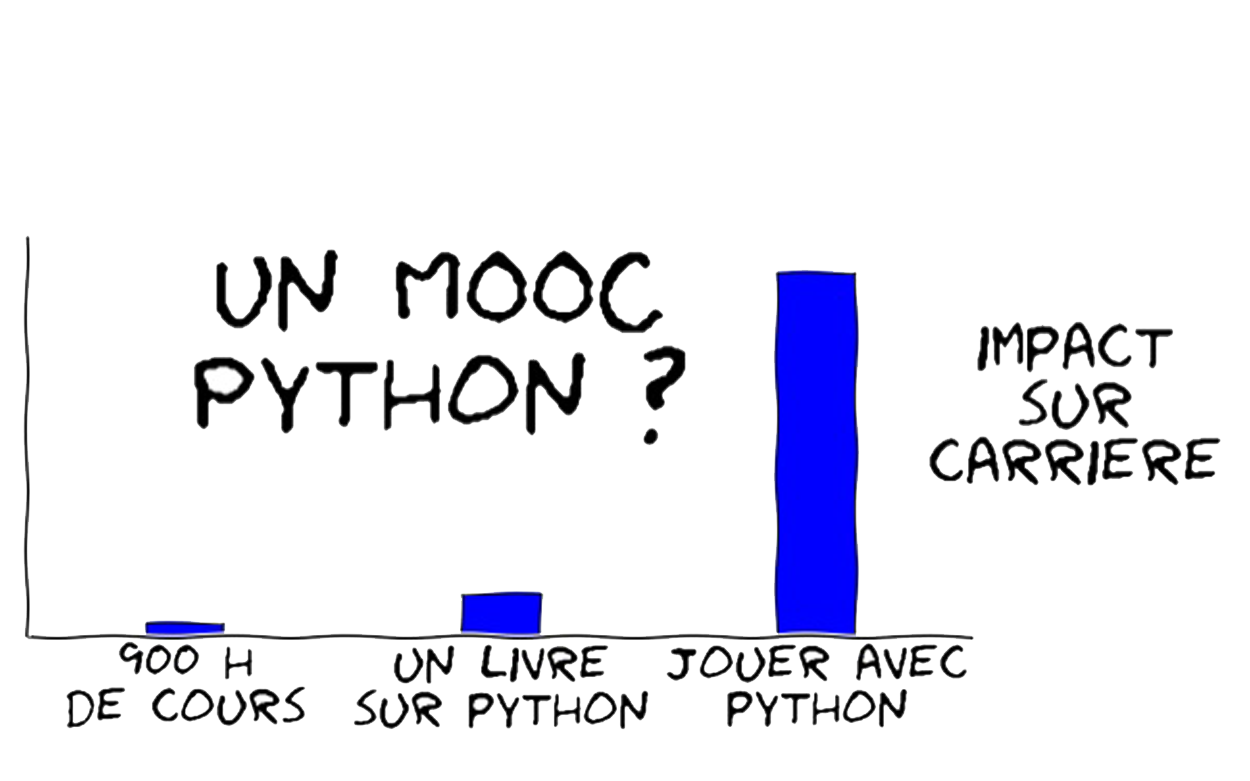
\includegraphics{medias/mooc2.png}\\
\vskip100pt

\includegraphics{medias/mooc.png}\\
\large https://www.fun-mooc.fr\\[0.5cm] % Minor heading
\large Licence CC BY-NC-ND Thierry Parmentelat et Arnaud Legout\\[0.5cm] % Minor heading

%----------------------------------------------------------------------------------------
%	DATE SECTION
%----------------------------------------------------------------------------------------

%{\large \today}\\[2cm] % Date, change the \today to a set date if you want to be precise

%----------------------------------------------------------------------------------------
%	LOGO SECTION
%----------------------------------------------------------------------------------------

%
\includegraphics{medias/logo.png}\\[1cm] 
 
%----------------------------------------------------------------------------------------

\vfill % Fill the rest of the page with whitespace

\end{titlepage}
  
\tableofcontents
    
    \chapter{Introduction au MOOC et aux outils Python}
    
	    \hypertarget{versions-de-python}{%
\section{Versions de Python}\label{versions-de-python}}

    \hypertarget{version-de-ruxe9fuxe9rence-python-3.6}{%
\subsubsection{Version de référence~:
Python-3.6}\label{version-de-ruxe9fuxe9rence-python-3.6}}

    Comme on l'indique dans la vidéo, la version de Python qui a servi de
\textbf{référence pour le MOOC est la version 3.6}, c'est notamment avec
cette version que l'on a tourné les vidéos.

    \hypertarget{versions-plus-anciennes}{%
\subsubsection{Versions plus anciennes}\label{versions-plus-anciennes}}

    Certaines précautions sont à prendre si vous utilisez une version plus
ancienne~:

    \hypertarget{python-3.5}{%
\subparagraph{Python-3.5}\label{python-3.5}}

    Si vous préférez utiliser python-3.5, la différence la plus visible pour
vous apparaitra avec les \emph{f-strings}~:

    \begin{Verbatim}[commandchars=\\\{\}]
{\color{incolor}In [{\color{incolor}1}]:} \PY{n}{age} \PY{o}{=} \PY{l+m+mi}{10}
        
        \PY{c+c1}{\PYZsh{} un exemple de f\PYZhy{}string}
        \PY{n}{f}\PY{l+s+s2}{\PYZdq{}}\PY{l+s+s2}{Jean a }\PY{l+s+si}{\PYZob{}age\PYZcb{}}\PY{l+s+s2}{ ans}\PY{l+s+s2}{\PYZdq{}}
\end{Verbatim}


\begin{Verbatim}[commandchars=\\\{\}]
{\color{outcolor}Out[{\color{outcolor}1}]:} 'Jean a 10 ans'
\end{Verbatim}
            
    Cette construction - que nous utilisons très fréquemment - n'a été
introduite qu'en Python-3.6, aussi si vous utilisez Python-3.5 vous
verrez ceci~:

\begin{Shaded}
\begin{Highlighting}[]
\OperatorTok{>>>}\NormalTok{ age }\OperatorTok{=} \DecValTok{10}
\OperatorTok{>>>} \SpecialStringTok{f"Jean a }\SpecialCharTok{\{}\NormalTok{age}\SpecialCharTok{\}}\SpecialStringTok{ ans"}
\NormalTok{  File }\StringTok{"<stdin>"}\NormalTok{, line }\DecValTok{1}
    \SpecialStringTok{f"Jean a }\SpecialCharTok{\{}\NormalTok{age}\SpecialCharTok{\}}\SpecialStringTok{ ans"}
                      \OperatorTok{^}
\PreprocessorTok{SyntaxError}\NormalTok{: invalid syntax}
\end{Highlighting}
\end{Shaded}

    Dans ce cas vous devrez remplacer ce code avec la méthode
\texttt{format} - que nous verrons en Semaine 2 avec les chaines de
caractères - et dans le cas présent il faudrait remplacer par ceci~:

    \begin{Verbatim}[commandchars=\\\{\}]
{\color{incolor}In [{\color{incolor}2}]:} \PY{n}{age} \PY{o}{=} \PY{l+m+mi}{10}
        
        \PY{l+s+s2}{\PYZdq{}}\PY{l+s+s2}{Jean a }\PY{l+s+si}{\PYZob{}\PYZcb{}}\PY{l+s+s2}{ ans}\PY{l+s+s2}{\PYZdq{}}\PY{o}{.}\PY{n}{format}\PY{p}{(}\PY{n}{age}\PY{p}{)}
\end{Verbatim}


\begin{Verbatim}[commandchars=\\\{\}]
{\color{outcolor}Out[{\color{outcolor}2}]:} 'Jean a 10 ans'
\end{Verbatim}
            
    Comme ces f-strings sont très présents dans le cours, il est recommandé
d'utiliser au moins python-3.6.

    \hypertarget{python-3.4}{%
\subparagraph{Python-3.4}\label{python-3.4}}

    La remarque vaut donc \emph{a fortiori} pour python-3.4 qui, en outre,
ne vous permettra pas de suivre la semaine 8 sur la programmation
asynchrone, car les mots-clés \texttt{async} et \texttt{await} ont été
introduits seulement dans Python-3.5.

    \hypertarget{version-utilisuxe9e-dans-les-notebooks-versions-plus-ruxe9centes}{%
\subsubsection{Version utilisée dans les notebooks / versions plus
récentes}\label{version-utilisuxe9e-dans-les-notebooks-versions-plus-ruxe9centes}}

    Tout le cours doit pouvoir s'exécuter tel quel avec une version plus
récente de Python.

Cela dit, certains compléments illustrent des nouveautés apparues après
la 3.6, comme les \emph{dataclasses} qui sont apparues avec python-3.7,
et que nous verrons en semaine 6.

Dans tous les cas, nous \textbf{signalons systématiquement} les
notebooks qui nécessitent une version plus récente que 3.6.

    Voici enfin, à toutes fins utiles, un premier fragment de code Python
qui affiche la version de Python utilisée dans tous les notebooks de ce
cours.

Nous reviendrons en détail sur l'utilisation des notebooks dans une
prochaine séquence, dans l'immédiat pour exécuter ce code vous pouvez~:
* désigner avec la souris la cellule de code~; vous verrez alors
apparaître une petite flèche à côté du mot \texttt{In}, en cliquant
cette flèche vous exécutez le code~; * une autre méthode consiste à
sélectionner la cellule de code avec la souris~; une fois que c'est fait
vous pouvez cliquer sur le bouton \texttt{\textgreater{}\textbar{}\ Run}
dans la barre de menu (bleue claire) du notebook.

    \begin{Verbatim}[commandchars=\\\{\}]
{\color{incolor}In [{\color{incolor}3}]:} \PY{c+c1}{\PYZsh{} ce premier fragment de code affiche des détails sur la}
        \PY{c+c1}{\PYZsh{} version de python qui exécute tous les notebooks du cours}
        \PY{k+kn}{import} \PY{n+nn}{sys}
        \PY{n+nb}{print}\PY{p}{(}\PY{n}{sys}\PY{o}{.}\PY{n}{version\PYZus{}info}\PY{p}{)}
\end{Verbatim}


    \begin{Verbatim}[commandchars=\\\{\}]
sys.version\_info(major=3, minor=6, micro=3, releaselevel='final', serial=0)

    \end{Verbatim}

    Pas de panique si vous n'y arrivez pas, nous consacrerons très bientôt
une séquence entière à l'utilisation des notebooks :)
    
    \hypertarget{installer-la-distribution-standard-python}{%
\section{Installer la distribution standard
Python}\label{installer-la-distribution-standard-python}}

    \hypertarget{compluxe9ment---niveau-basique}{%
\subsection{Complément - niveau
basique}\label{compluxe9ment---niveau-basique}}

    Ce complément a pour but de vous donner quelques guides pour
l'installation de la distribution standard Python 3.

Notez bien qu'il ne s'agit ici que d'indications, il existe de
nombreuses façons de procéder.

En cas de souci, commencez par chercher par vous-même, sur google ou
autre, une solution à votre problème~; pensez également à utiliser le
forum du cours.

    Le point important est de \textbf{bien vérifier le numéro de version} de
votre installation qui doit être \textbf{au moins 3.6}

    \hypertarget{sachez-uxe0-qui-vous-parlez}{%
\subsection{Sachez à qui vous
parlez}\label{sachez-uxe0-qui-vous-parlez}}

    Mais avant qu'on n'avance sur l'installation proprement dite, il nous
faut insister sur un point qui déroute parfois les débutants. On a
parfois besoin de recourir à l'emploi d'un terminal, surtout justement
pendant la phase d'installation.\\

Lorsque c'est le cas, il est important de bien distinguer~:

\begin{itemize}
\item
	les cas où on s'adresse \textbf{au terminal} (en jargon, on dit le \emph{shell}),
\item	
	et les cas où on s'adresse à \textbf{l'interpréteur Python}.
\end{itemize}


C'est très important car ces deux programmes ne parlent \textbf{pas} du
tout le \textbf{même langage} ! Il peut arriver au début qu'on écrive
une commande juste, mais au mauvais interlocuteur, et cela peut être
source de frustration. Essayons de bien comprendre ce point.

    \hypertarget{le-terminal}{%
\subsubsection{Le terminal}\label{le-terminal}}

Je peux dire que je parle à mon \textbf{terminal} quand l'invite de
commande (en jargon on dit le \emph{prompt}) \textbf{se termine par un
dollar \texttt{\$}} - ou un simple chevron \texttt{\textgreater{}} sur
Windows

Par exemple~sur un mac :

\begin{verbatim}
~/git/flotpython/w1 $ 
\end{verbatim}

Ou sur Windows~:

\begin{verbatim}
C:\Users>        
\end{verbatim}

    \hypertarget{linterpruxe8te-python}{%
\subsubsection{L'interprète Python}\label{linterpruxe8te-python}}

À partir du terminal, je peux lancer un \textbf{interpréteur Python},
qui se reconnaît car son prompt est fait de \textbf{3 chevrons
\texttt{\textgreater{}\textgreater{}\textgreater{}}}

\begin{verbatim}
~/git/flotpython/w1 $ python3
Python 3.7.0 (default, Jun 29 2018, 20:14:27)
[Clang 9.0.0 (clang-900.0.39.2)] on darwin
Type "help", "copyright", "credits" or "license" for more information.
>>>
\end{verbatim}

    Pour sortir de l'interpréteur Python, et retourner au terminal,
j'utilise la fonction Python \texttt{exit()}~:

\begin{verbatim}
~/git/flotpython/w1 $ python3
>>> 20 * 60
1200
>>> exit()
~/git/flotpython/w1 $ python3
\end{verbatim}

    \hypertarget{les-erreurs-typiques}{%
\subsubsection{Les erreurs typiques}\label{les-erreurs-typiques}}

Gardez bien cette distinction présente à l'esprit, lorsque vous lisez la
suite. Voici quelques symptômes habituels de ce qu'on obtient si on se
trompe.

Par exemple, la commande \texttt{python3\ -V} est une commande qui
s'adresse au terminal; c'est pourquoi nous la faisons précéder d'un
dollar \texttt{\$}.

Si vous essayez de la taper alors que vous êtes déjà dans un
interpréteur python - ou sous IDLE d'ailleurs -, vous obtenez un message
d'erreur de ce genre :

\begin{verbatim}
>>> python3 -V
Traceback (most recent call last):
  File "<stdin>", line 1, in <module>
NameError: name 'python3' is not defined
\end{verbatim}

    Réciproquement, si vous essayez de taper du Python directement dans un
terminal, ça se passe mal aussi, forcément. Par exemple sur Mac, avec
des fragments Python tout simples~:

\begin{verbatim}
~/git/flotpython/w1 $ import math
-bash: import: command not found
~/git/flotpython/w1 $ 30 * 60
-bash: 30: command not found
~/git/flotpython/w1 $ foo = 30 * 60
-bash: foo: command not found
\end{verbatim}

    \hypertarget{digression---coexistence-de-python2-et-python3}{%
\subsection{Digression - coexistence de Python2 et
Python3}\label{digression---coexistence-de-python2-et-python3}}

    Avant l'arrivée de la version 3 de Python, les choses étaient simples,
on exécutait un programme Python avec une seule commande
\texttt{python}. Depuis 2014-2015, maintenant que les deux versions de
Python coexistent, il est nécessaire d'adopter une convention qui
permette d'installer les deux langages sous des noms qui sont
non-ambigus.\\

C'est pourquoi actuellement, on trouve \textbf{le plus souvent} la
convention suivante sous Linux et macOS~:

\begin{itemize}
\item
  \texttt{python3} est pour exécuter les programmes en Python-3~; du
  coup on trouve alors également les commandes comme \texttt{idle3} pour
  lancer IDLE, et par exemple \texttt{pip3} pour le gestionnaire de
  paquets (voir ci-dessous)~;
\item
  \texttt{python2} est pour exécuter les programmes en Python-2, avec
  typiquement \texttt{idle2} et \texttt{pip2}~;
\item
  enfin selon les systèmes, la commande \texttt{python} tout court est
  un alias pour \texttt{python2} ou \texttt{python3}. De plus en plus
  souvent, par défaut \texttt{python} désigne \texttt{python3}.
\end{itemize}

à titre d'illustration, voici ce que j'obtiens sur mon mac~:

\begin{verbatim}
$ python3 -V
Python 3.6.2
$ python2 -V
Python 2.7.13
$ python -V
Python 3.6.2
\end{verbatim}

Sous Windows, vous avez un lanceur qui s'appelle \texttt{py}. Par
défaut, il lance la version de Python la plus récente installée, mais
vous pouvez spécifier une version spécifique de la manière suivante~:

\begin{verbatim}
C:\> py -2.7
\end{verbatim}

pour lancer, par exemple, Python en version 2.7. Vous trouverez toute la
documentation nécessaire pour Windows sur cette page (en anglais)~:
\href{https://docs.python.org/3/using/windows.html}{https://docs.python.org/3/using/windows.html}\\

Pour éviter d'éventuelles confusions, nous précisons toujours
\texttt{python3} dans le cours.

    \hypertarget{installation-de-base}{%
\subsection{Installation de base}\label{installation-de-base}}

    \hypertarget{vous-utilisez-windows}{%
\subsubsection{Vous utilisez Windows}\label{vous-utilisez-windows}}

    La méthode recommandée sur Windows est de partir de la page
\href{https://www.python.org/download}{https://www.python.org/download} où vous trouverez un programme
d'installation qui contient tout ce dont vous aurez besoin pour suivre
le cours.\\

Pour vérifier que vous êtes prêts, il vous faut lancer IDLE (quelque
part dans le menu Démarrer) et vérifier le numéro de version.

    \hypertarget{vous-utilisez-macos}{%
\subsubsection{Vous utilisez macOS}\label{vous-utilisez-macos}}

    Ici encore, la méthode recommandée est de partir de la page
\href{https://www.python.org/download}{www.python.org/download} et d'utiliser le programme
d'installation.\\

Sachez aussi, si vous utilisez déjà MacPorts (\href{https://www.macports.org}{https://www.macports.org}),
que vous pouvez également utiliser cet outil pour installer, par exemple
Python 3.6, avec la commande

    \begin{verbatim}
$ sudo port install python36
\end{verbatim}

    \hypertarget{vous-utilisez-linux}{%
\subsubsection{Vous utilisez Linux}\label{vous-utilisez-linux}}

    Dans ce cas il est très probable que Python-3.x soit déjà disponible sur
votre machine. Pour vous en assurer, essayez de lancer la commande
\texttt{python3} dans un terminal.\\

\textbf{RHEL / Fedora}\\


Voici par exemple ce qu'on obtient depuis un terminal sur une machine
installée en Fedora-20~:

    \begin{verbatim}
$ python3
Python 3.6.2 (default, Jul 20 2017, 12:30:02)
[GCC 6.3.1 20161221 (Red Hat 6.3.1-1)] on linux
Type "help", "copyright", "credits" or "license" for more information.
>>> exit()
\end{verbatim}

    \textbf{Vérifiez bien le numéro de version} qui doit être en 3.\emph{x}.
Si vous obtenez un message du style
\texttt{python3:\ command\ not\ found} utilisez \texttt{dnf}
(anciennement connu sous le nom de \texttt{yum}) pour installer le rpm
\texttt{python3} comme ceci~:

    \begin{verbatim}
$ sudo dnf install python3
\end{verbatim}

    S'agissant d'\texttt{idle}, l'éditeur que nous utilisons dans le cours
(optionnel si vous êtes familier avec un éditeur de texte), vérifiez sa
présence comme ceci~:

    \begin{verbatim}
$ type idle3
idle is hashed (/usr/bin/idle3)
\end{verbatim}

    Ici encore, si la commande n'est pas disponible vous pouvez l'installer
avec~:

    \begin{verbatim}
$ sudo yum install python3-tools
\end{verbatim}


\textbf{Debian / Ubuntu}\\

    Ici encore, Python-2.7 est sans doute déjà disponible. Procédez comme
ci-dessus, voici un exemple recueilli dans un terminal sur une machine
installée en Ubuntu-14.04/trusty~:

    \begin{verbatim}
$ python3
Python 3.6.2 (default, Jul 20 2017, 12:30:02)
[GCC 6.3.1 20161221 (Red Hat 6.3.1-1)] on linux
Type "help", "copyright", "credits" or "license" for more information.
>>> exit()
\end{verbatim}

    Pour installer Python~:

    \begin{verbatim}
$ sudo apt-get install python3
\end{verbatim}

    Pour installer idle~:

    \begin{verbatim}
$ sudo apt-get install idle3
\end{verbatim}

    \hypertarget{installation-de-bibliothuxe8ques-compluxe9mentaires}{%
\subsubsection{Installation de bibliothèques
complémentaires}\label{installation-de-bibliothuxe8ques-compluxe9mentaires}}

    Il existe un outil très pratique pour installer des bibliothèques
Python, il s'appelle \texttt{pip3}, qui est documenté ici
\href{https://pypi.python.org/pypi/pip}{https://pypi.python.org/pypi/pip}\\

    Sachez aussi, si par ailleurs vous utilisez un gestionnaire de paquets
comme \texttt{rpm} sur RHEL, \texttt{apt-get} sur Debian, ou
\texttt{port} sur macOS, que de nombreux paquets sont également
disponibles au travers de ces outils.

    \hypertarget{anaconda}{%
\subsubsection{Anaconda}\label{anaconda}}

    Sachez qu'il existe beaucoup de distributions alternatives qui incluent
Python~; parmi elles, la plus populaire est sans aucun doute
\href{https://www.anaconda.com/}{Anaconda}, qui contient un grand nombre
de bibliothèques de calcul scientifique, et également d'ailleurs jupyter
pour travailler nativement sur des notebooks au format \texttt{.ipynb}.\\

Anaconda vient avec son propre gestionnaires de paquets pour
l'installation de bibliothèques supplémentaires qui s'appelle
\texttt{conda}.
        \hypertarget{un-peu-de-lecture}{%
\section{Un peu de lecture}\label{un-peu-de-lecture}}

    \hypertarget{compluxe9ment---niveau-basique}{%
\subsection{Complément - niveau
basique}\label{compluxe9ment---niveau-basique}}

    \hypertarget{mise-uxe0-jour-de-juillet-2018}{%
\subsubsection{Mise à jour de Juillet
2018}\label{mise-uxe0-jour-de-juillet-2018}}

    Le 12 Juillet 2018, Guido van Rossum
\href{https://lwn.net/Articles/759654/}{a annoncé qu'il quittait la
fonction de BDFL} qu'il occupait depuis près de trois décennies. Il
n'est pas tout à fait clair à ce stade comment va évoluer la gouvernance
de Python.

    \hypertarget{le-zen-de-python}{%
\subsubsection{Le Zen de Python}\label{le-zen-de-python}}

    Vous pouvez lire le ``Zen de Python'', qui résume la philosophie du
langage, en important le module \texttt{this} avec ce code~: (pour
exécuter ce code, cliquez dans la cellule de code, et faites au clavier
``Majuscule/Entrée'' ou ``Shift/Enter'')

    \begin{Verbatim}[commandchars=\\\{\}]
{\color{incolor}In [{\color{incolor}1}]:} \PY{c+c1}{\PYZsh{} le Zen de Python}
        \PY{k+kn}{import} \PY{n+nn}{this}
\end{Verbatim}


    \begin{Verbatim}[commandchars=\\\{\}]
The Zen of Python, by Tim Peters

Beautiful is better than ugly.
Explicit is better than implicit.
Simple is better than complex.
Complex is better than complicated.
Flat is better than nested.
Sparse is better than dense.
Readability counts.
Special cases aren't special enough to break the rules.
Although practicality beats purity.
Errors should never pass silently.
Unless explicitly silenced.
In the face of ambiguity, refuse the temptation to guess.
There should be one-- and preferably only one --obvious way to do it.
Although that way may not be obvious at first unless you're Dutch.
Now is better than never.
Although never is often better than *right* now.
If the implementation is hard to explain, it's a bad idea.
If the implementation is easy to explain, it may be a good idea.
Namespaces are one honking great idea -- let's do more of those!

    \end{Verbatim}

    \hypertarget{documentation}{%
\subsubsection{Documentation}\label{documentation}}

    \begin{itemize}
\item
  On peut commencer par citer
  l'\href{http://fr.wikipedia.org/wiki/Python_\%28langage\%29}{article
  de Wikipédia sur Python en français}.
\item
  La \href{https://wiki.python.org/moin/FrenchLanguage}{page sur le
  langage en français}.
\item
  La \href{https://docs.python.org/3/}{documentation originale} de
  Python 3 - donc, en anglais - est un très bon point d'entrée lorsqu'on
  cherche un sujet particulier, mais (beaucoup) trop abondante pour être
  lue d'un seul trait. Pour chercher de la documentation sur un module
  particulier, le plus simple est encore d'utiliser Google - ou votre
  moteur de recherche favori - qui vous redirigera, dans la grande
  majorité des cas, vers la page qui va bien dans, précisément, la
  documentation de Python.

  À titre d'exercice, cherchez la documentation du module
  \texttt{pathlib} en
  \href{https://www.google.fr/search?q=python+module+pathlib}{cherchant
  sur Google} les mots-clé \texttt{"python\ module\ pathlib"}.
\item
  J'aimerais vous signaler également une initiative pour
  \href{https://docs.python.org/fr/3/}{traduire la documentation
  officielle en français}.
\end{itemize}

    \hypertarget{historique-et-survol}{%
\subsubsection{Historique et survol}\label{historique-et-survol}}

    \begin{itemize}
\tightlist
\item
  La FAQ officielle de Python (en anglais) sur
  \href{https://docs.python.org/3/faq/design.html}{les choix de
  conception et l'historique du langage}.
\item
  L'article de Wikipédia (en anglais) sur
  l'\href{http://en.wikipedia.org/wiki/History_of_Python}{historique du
  langage}.
\item
  Sur Wikipédia, un article (en anglais) sur
  \href{http://en.wikipedia.org/wiki/Python_syntax_and_semantics}{la
  syntaxe et la sémantique de Python}.
\end{itemize}

    \hypertarget{un-peu-de-folklore}{%
\subsubsection{Un peu de folklore}\label{un-peu-de-folklore}}

    \begin{itemize}
\tightlist
\item
  Le \href{https://www.youtube.com/watch?v=YgtL4S7Hrwo}{discours de
  Guido van Rossum à PyCon 2016}.
\item
  Sur YouTube, le
  \href{https://www.youtube.com/watch?v=anwy2MPT5RE}{sketch des Monty
  Python} d'où proviennent les termes \texttt{spam}, \texttt{eggs} et
  autres \texttt{beans} que l'on utilise traditionnellement dans les
  exemples en Python plutôt que \texttt{foo} et \texttt{bar}.
\item
  L'\href{http://en.wikipedia.org/wiki/Spam_\%28Monty_Python\%29}{article
  Wikipédia correspondant}, qui cite le langage Python.
\end{itemize}

    \hypertarget{compluxe9ment---niveau-intermuxe9diaire}{%
\subsection{Complément - niveau
intermédiaire}\label{compluxe9ment---niveau-intermuxe9diaire}}

    \hypertarget{licence}{%
\subsubsection{Licence}\label{licence}}

    \begin{itemize}
\tightlist
\item
  La \href{https://docs.python.org/3/license.html}{licence d'utilisation
  est disponible ici}.
\item
  La page de la \href{https://www.python.org/psf/}{Python Software
  Foundation}, qui est une entité légale similaire à nos associations de
  1901, à but non lucratif~; elle possède les droits sur le langage.
\end{itemize}

    \hypertarget{le-processus-de-duxe9veloppement}{%
\subsubsection{Le processus de
développement}\label{le-processus-de-duxe9veloppement}}

    \begin{itemize}
\tightlist
\item
  Comment les choix d'évolution sont proposés et discutés, au travers
  des PEP (Python Enhancement Proposals)

  \begin{itemize}
  \tightlist
  \item
    \href{http://en.wikipedia.org/wiki/Python\_(programming\_language)\#Development}{http://en.wikipedia.org/wiki/Python\_(programming\_language)\#Development}
  \end{itemize}
\item
  Le premier PEP décrit en détail le cycle de vie des PEPs

  \begin{itemize}
  \tightlist
  \item
    \href{http://legacy.python.org/dev/peps/pep-0001/}{http://legacy.python.org/dev/peps/pep-0001/}
  \end{itemize}
\item
  Le PEP 8, qui préconise un style de présentation (\emph{style guide})

  \begin{itemize}
  \tightlist
  \item
    \href{http://legacy.python.org/dev/peps/pep-0008/}{http://legacy.python.org/dev/peps/pep-0008/}
  \end{itemize}
\item
  L'index de tous les PEPs

  \begin{itemize}
  \tightlist
  \item
    \href{http://legacy.python.org/dev/peps/}{http://legacy.python.org/dev/peps/}
  \end{itemize}
\end{itemize}
        \hypertarget{notebooks-jupyter-comme-support-de-cours}{%
\section{``Notebooks'' Jupyter comme support de
cours}\label{notebooks-jupyter-comme-support-de-cours}}

    Pour illustrer les vidéos du MOOC, nous avons choisi d'utiliser Jupyter
pour vous rédiger les documents ``mixtes'' contenant du texte et du code
Python, qu'on appelle des ``notebooks'', et dont le présent document est
un exemple.

Nous allons, dans la suite, utiliser du code Python, pourtant nous
n'avons pas encore abordé le langage. Pas d'inquiétude, ce code est
uniquement destiné à valider le fonctionnement des notebooks, et nous
n'utilisons que des choses très simples.

    \hypertarget{avertissement-ruxe9glages-du-navigateur}{%
\subsubsection{Avertissement: réglages du
navigateur}\label{avertissement-ruxe9glages-du-navigateur}}

    Avant toute chose, pour un bon fonctionnement des notebooks, on rappelle
qu'il est nécessaire d'avoir \textbf{autorisé} dans votre navigateur les
\textbf{cookies} en provenance du site Internet
\textbf{\texttt{nbhosting.inria.fr}}, qui héberge l'infrastructure qui
héberge tous les notebooks.

    \hypertarget{avantages-des-notebooks}{%
\subsubsection{Avantages des notebooks}\label{avantages-des-notebooks}}

    Comme vous le voyez, ce support permet un format plus lisible que des
commentaires dans un fichier de code.

    Nous attirons votre attention sur le fait que \textbf{les fragments de
code peuvent être évalués et modifiés}. Ainsi vous pouvez facilement
essayer des variantes autour du notebook original.

Notez bien également que le code Python est interprété \textbf{sur une
machine distante}, ce qui vous permet de faire vos premiers pas avant
même d'avoir procédé à l'installation de Python sur votre propre
ordinateur.

    \hypertarget{comment-utiliser-les-notebooks}{%
\subsubsection{Comment utiliser les
notebooks}\label{comment-utiliser-les-notebooks}}

    En haut du notebook, vous avez une barre de menu (sur fond bleu clair),
contenant~:

\begin{itemize}
	\item
un titre pour le notebook, avec un numéro de version~;
	\item
une barre de menus avec les entrées \texttt{File}, \texttt{Insert},
\texttt{Cell}, \texttt{Kernel};
	\item
et une barre de boutons qui sont des
raccourcis vers certains menus fréquemment utilisés. Si vous laissez
votre souris au dessus d'un bouton, un petit texte apparaît, indiquant à
quelle fonction correspond ce bouton.
\end{itemize}

Nous avons vu dans la vidéo qu'un notebook est constitué d'une suite de
cellules, soit textuelles, soit contenant du code. Les cellules de code
sont facilement reconnaissables, elles sont précédées de
\texttt{In\ {[}\ {]}:}. La cellule qui suit celle que vous êtes en train
de lire est une cellule de code.

Pour commencer, sélectionnez cette cellule de code avec votre souris, et
appuyez dans la barre de menu - en haut du notebook, donc - sur celui en
forme de flèche triangulaire vers la droite (Play)~: 

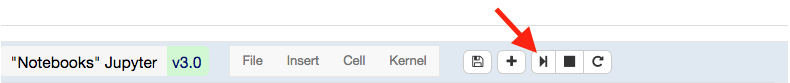
\includegraphics{medias/notebook-eval-button.png}\\
    \begin{Verbatim}[commandchars=\\\{\}]
{\color{incolor}In [{\color{incolor}1}]:} \PY{l+m+mi}{20} \PY{o}{*} \PY{l+m+mi}{30}
\end{Verbatim}


\begin{Verbatim}[commandchars=\\\{\}]
{\color{outcolor}Out[{\color{outcolor}1}]:} 600
\end{Verbatim}
            
    Comme vous le voyez, la cellule est ``exécutée'' (on dira plus
volontiers évaluée), et on passe à la cellule suivante.

Alternativement, vous pouvez simplement taper au clavier
\textbf{\emph{Shift+Enter}}, ou selon les claviers
\textbf{\emph{Maj-Entrée}}, pour obtenir le même effet. D'une manière
générale, il est important d'apprendre et d'utiliser les raccourcis
clavier, cela vous fera gagner beaucoup de temps par la suite.

    La façon habituelle d'\emph{exécuter} l'ensemble du notebook consiste~:
\begin{itemize}
	\item
	à sélectionner la première cellule,
	\item
	et à taper \textbf{\emph{Shift+Enter}} jusqu'à attendre la fin du notebook.
\end{itemize}

    Lorsqu'une cellule de code a été évaluée, Jupyter ajoute sous la cellule
\texttt{In} une cellule \texttt{Out} qui donne le résultat du fragment
Python, soit ci-dessus 600.\\

Jupyter ajoute également un nombre entre les crochets pour afficher, par
exemple ci-dessus, \texttt{In\ {[}1{]}:}. Ce nombre vous permet de
retrouver l'ordre dans lequel les cellules ont été évaluées.

    Vous pouvez naturellement modifier ces cellules de code pour faire des
essais~; ainsi vous pouvez vous servir du modèle ci-dessous pour
calculer la racine carrée de 3, ou essayer la fonction sur un nombre
négatif et voir comment est signalée l'erreur.

    \begin{Verbatim}[commandchars=\\\{\}]
{\color{incolor}In [{\color{incolor}2}]:} \PY{c+c1}{\PYZsh{} math.sqrt (pour square root) calcule la racine carrée}
        \PY{k+kn}{import} \PY{n+nn}{math}
        \PY{n}{math}\PY{o}{.}\PY{n}{sqrt}\PY{p}{(}\PY{l+m+mi}{2}\PY{p}{)}
\end{Verbatim}


\begin{Verbatim}[commandchars=\\\{\}]
{\color{outcolor}Out[{\color{outcolor}2}]:} 1.4142135623730951
\end{Verbatim}
            
    On peut également évaluer tout le notebook en une seule fois en
utilisant le menu \emph{Cell -\textgreater{} Run All}.

    \hypertarget{attention-uxe0-bien-uxe9valuer-les-cellules-dans-lordre}{%
\subsubsection{Attention à bien évaluer les cellules dans
l'ordre}\label{attention-uxe0-bien-uxe9valuer-les-cellules-dans-lordre}}

    Il est important que les cellules de code soient évaluées dans le bon
ordre. Si vous ne respectez pas l'ordre dans lequel les cellules de code
sont présentées, le résultat peut être inattendu.\\

En fait, évaluer un programme sous forme de notebook revient à le
découper en petits fragments, et si on exécute ces fragments dans le
désordre, on obtient naturellement un programme différent.

    On le voit sur cet exemple~:

    \begin{Verbatim}[commandchars=\\\{\}]
{\color{incolor}In [{\color{incolor}3}]:} \PY{n}{message} \PY{o}{=} \PY{l+s+s2}{\PYZdq{}}\PY{l+s+s2}{Il faut faire attention à l}\PY{l+s+s2}{\PYZsq{}}\PY{l+s+s2}{ordre dans lequel on évalue les notebooks}\PY{l+s+s2}{\PYZdq{}}
\end{Verbatim}


    \begin{Verbatim}[commandchars=\\\{\}]
{\color{incolor}In [{\color{incolor}4}]:} \PY{n+nb}{print}\PY{p}{(}\PY{n}{message}\PY{p}{)}
\end{Verbatim}


    \begin{Verbatim}[commandchars=\\\{\}]
Il faut faire attention à l'ordre dans lequel on évalue les notebooks

    \end{Verbatim}

    Si un peu plus loin dans le notebook on fait par exemple~:

    \begin{Verbatim}[commandchars=\\\{\}]
{\color{incolor}In [{\color{incolor}5}]:} \PY{c+c1}{\PYZsh{} ceci a pour effet d\PYZsq{}effacer la variable \PYZsq{}message\PYZsq{}}
        \PY{k}{del} \PY{n}{message}
\end{Verbatim}


    qui rend le symbole \texttt{message} indéfini, alors bien sûr on ne peut
plus évaluer la cellule qui fait \texttt{print} puisque la variable
\texttt{message} n'est plus connue de l'interpréteur.

    \hypertarget{ruxe9initialiser-linterpruxe9teur}{%
\subsubsection{Réinitialiser
l'interpréteur}\label{ruxe9initialiser-linterpruxe9teur}}

    Si vous faites trop de modifications, ou perdez le fil de ce que vous
avez évalué, il peut être utile de redémarrer votre interpréteur. Le
menu \emph{Kernel~→~Restart} vous permet de faire cela, un peu à la
manière de IDLE qui repart d'un interpréteur vierge lorsque vous
utilisez la fonction F5.

    Le menu \emph{Kernel~→~Interrupt} peut être quant à lui utilisé si votre
fragment prend trop longtemps à s'exécuter (par exemple vous avez écrit
une boucle dont la logique est cassée et qui ne termine pas).

    \hypertarget{vous-travaillez-sur-une-copie}{%
\subsubsection{Vous travaillez sur une
copie}\label{vous-travaillez-sur-une-copie}}

    Un des avantages principaux des notebooks est de vous permettre de
modifier le code que nous avons écrit, et de voir par vous-mêmes comment
se comporte le code modifié.\\

Pour cette raison, chaque élève dispose de sa \textbf{propre copie} de
chaque notebook, vous pouvez bien sûr apporter toutes les modifications
que vous souhaitez à vos notebooks sans affecter les autres étudiants.

    \hypertarget{revenir-uxe0-la-version-du-cours}{%
\subsubsection{Revenir à la version du
cours}\label{revenir-uxe0-la-version-du-cours}}

    Vous pouvez toujours revenir à la version ``du cours'' grâce au menu
\emph{File~→~Reset to original}.\\

    Attention, avec cette fonction vous restaurez \textbf{tout le notebook}
et donc \textbf{vous perdez vos modifications sur ce notebook}.

    \hypertarget{tuxe9luxe9charger-au-format-python}{%
\subsubsection{Télécharger au format
Python}\label{tuxe9luxe9charger-au-format-python}}

    Vous pouvez télécharger un notebook au format Python sur votre
ordinateur grâce au menu \emph{File~→~Download~as~→~Python}

    Les cellules de texte sont préservées dans le résultat sous forme de
commentaires Python.

    \hypertarget{partager-un-notebook-en-lecture-seule}{%
\subsubsection{Partager un notebook en lecture
seule}\label{partager-un-notebook-en-lecture-seule}}

    Enfin, avec le menu \emph{File~→~Share~static~version}, vous pouvez
publier une version en lecture seule de votre notebook~; vous obtenez
une URL que vous pouvez publier, par exemple pour demander de l'aide sur
le forum. Ainsi, les autres étudiants peuvent accéder en lecture seule à
votre code.\\

    Notez que lorsque vous utilisez cette fonction plusieurs fois, c'est
toujours la dernière version publiée que verront vos camarades, l'URL
utilisée reste toujours la même pour un étudiant et un notebook donné.

    \hypertarget{ajouter-des-cellules}{%
\subsubsection{Ajouter des cellules}\label{ajouter-des-cellules}}

    Vous pouvez ajouter une cellule n'importe où dans le document avec le
bouton \textbf{+} de la barre de boutons.\\

Aussi, lorsque vous arrivez à la fin du document, une nouvelle cellule
est créée chaque fois que vous évaluez la dernière cellule~; de cette
façon vous disposez d'un brouillon pour vos propres essais.\\

À vous de jouer.

        \hypertarget{modes-dexuxe9cution}{%
\section{Modes d'exécution}\label{modes-dexuxe9cution}}

    Nous avons donc à notre disposition plusieurs façons d'exécuter un
programme Python. Nous allons les étudier plus en détail~:

    \begin{longtable}[]{@{}ll@{}}
\toprule
Quoi & Avec quel outil\tabularnewline
\midrule
\endhead
fichier complet &
\texttt{python3\ \textless{}fichier\textgreater{}.py}\tabularnewline
ligne à ligne & \texttt{python3} en mode interactif\tabularnewline
~ & ou sous \texttt{ipython3}\tabularnewline
~ & ou avec IDLE\tabularnewline
par fragments & dans un notebook\tabularnewline
\bottomrule
\end{longtable}

    Pour cela nous allons voir le comportement d'un tout petit programme
Python lorsqu'on l'exécute sous ces différents environnements.\\

On veut surtout expliquer une petite différence quant au niveau de
détail de ce qui se trouve imprimé.\\

    Essentiellement, lorsqu'on utilise l'interpréteur en mode interactif -
ou sous IDLE - à chaque fois que l'on tape une ligne, le résultat est
\textbf{calculé} (on dit aussi \textbf{évalué}) puis \textbf{imprimé}.\\

Par contre, lorsqu'on écrit tout un programme, on ne peut plus imprimer
le résultat de toutes les lignes, cela produirait un flot d'impression
beaucoup trop important. Par conséquent, si vous ne déclenchez pas une
impression avec, par exemple, la fonction \texttt{print}, rien ne
s'affichera.\\

Enfin, en ce qui concerne le notebook, le comportement est un peu
hybride entre les deux, en ce sens que seul le \textbf{dernier résultat}
de la cellule est imprimé.

    \hypertarget{linterpruxe9teur-python-interactif}{%
\subsubsection{L'interpréteur Python
interactif}\label{linterpruxe9teur-python-interactif}}

    Le programme choisi est très simple, c'est le suivant~:

    \begin{Shaded}
\begin{Highlighting}[]
\DecValTok{10} \OperatorTok{*} \DecValTok{10}
\DecValTok{20} \OperatorTok{*} \DecValTok{20}
\DecValTok{30} \OperatorTok{*} \DecValTok{30}
\end{Highlighting}
\end{Shaded}

    Voici comment se comporte l'interpréteur interactif quand on lui soumet
ces instructions~:

    \begin{verbatim}
$ python3
Python 3.5.1 (v3.5.1:37a07cee5969, Dec  5 2015, 21:12:44)
[GCC 4.2.1 (Apple Inc. build 5666) (dot 3)] on darwin
Type "help", "copyright", "credits" or "license" for more information.
>>> 10 * 10
100
>>> 20 * 20
400
>>> 30 * 30
900
>>> exit()
$
\end{verbatim}

    Notez que pour terminer la session, il nous faut ``sortir'' de
l'interpréteur en tapant \texttt{exit()}.\\

On peut aussi taper \texttt{Control-D} sous Linux ou macOS.\\

    Comme on le voit ici, l'interpréteur imprime \textbf{le résultat de
chaque ligne}. On voit bien apparaître toutes les valeurs calculées,
100, 400, puis enfin 900.

    \hypertarget{sous-forme-de-programme-constituuxe9}{%
\subsubsection{Sous forme de programme
constitué}\label{sous-forme-de-programme-constituuxe9}}

    Voyons à présent ce que donne cette même séquence de calculs dans un
programme complet. Pour cela, il nous faut tout d'abord fabriquer un
fichier avec un suffixe en \texttt{.py}, en utilisant par exemple un
éditeur de fichier. Le résultat doit ressembler à ceci~:

    \begin{verbatim}
$ cat foo.py
10 * 10
20 * 20
30 * 30
$
\end{verbatim}

    Exécutons à présent ce programme~:

    \begin{verbatim}
$ python3 foo.py
$
\end{verbatim}

    On constate donc que ce programme \textbf{ne fait rien~!} En tout cas,
selon toute apparence.\\

En réalité, les 3 valeurs 100, 400 et 900 sont bien calculées, mais
comme aucune instruction \texttt{print} n'est présente, rien n'est
imprimé et le programme se termine sans signe apparent d'avoir
réellement fonctionné.\\

Ce comportement peut paraître un peu déroutant au début, mais comme nous
l'avons mentionné c'est tout à fait délibéré. Un programme fonctionnel
faisant facilement plusieurs milliers de lignes, voire beaucoup plus, il
ne serait pas du tout réaliste que chaque ligne produise une impression,
comme c'est le cas en mode interactif.

    \hypertarget{dans-un-notebook}{%
\subsubsection{Dans un notebook}\label{dans-un-notebook}}

    Voici à présent le même programme dans un notebook~:

    \begin{Verbatim}[commandchars=\\\{\}]
{\color{incolor}In [{\color{incolor}1}]:} \PY{l+m+mi}{10} \PY{o}{*} \PY{l+m+mi}{10}
        \PY{l+m+mi}{20} \PY{o}{*} \PY{l+m+mi}{20}
        \PY{l+m+mi}{30} \PY{o}{*} \PY{l+m+mi}{30}
\end{Verbatim}


\begin{Verbatim}[commandchars=\\\{\}]
{\color{outcolor}Out[{\color{outcolor}1}]:} 900
\end{Verbatim}
            
    Lorsqu'on exécute cette cellule (rappel~: sélectionner la cellule, et
utiliser le bouton en forme de flèche vers la droite, ou entrer
\textbf{``Shift+Enter''} au clavier), on obtient une seule valeur dans
la rubrique \texttt{Out{[}{]}}, 900, qui correspond \textbf{au résultat
de la dernière ligne.}

    \hypertarget{utiliser-print}{%
\subsubsection{\texorpdfstring{Utiliser
\texttt{print}}{Utiliser print}}\label{utiliser-print}}

    Ainsi, pour afficher un résultat intermédiaire, on utilise l'instruction
\texttt{print}. Nous verrons cette instruction en détail dans les
semaines qui viennent, mais en guise d'introduction disons seulement que
c'est une fonction comme les autres en Python 3.

    \begin{Verbatim}[commandchars=\\\{\}]
{\color{incolor}In [{\color{incolor}2}]:} \PY{n}{a} \PY{o}{=} \PY{l+m+mi}{10}
        \PY{n}{b} \PY{o}{=} \PY{l+m+mi}{20}
        
        \PY{n+nb}{print}\PY{p}{(}\PY{n}{a}\PY{p}{,} \PY{n}{b}\PY{p}{)}
\end{Verbatim}


    \begin{Verbatim}[commandchars=\\\{\}]
10 20

    \end{Verbatim}

    On peut naturellement mélanger des objets de plusieurs types, et donc
mélanger des chaînes de caractères et des nombres pour obtenir un
résultat un peu plus lisible. En effet, lorsque le programme devient
gros, il est important de savoir à quoi correspond une ligne dans le
flot de toutes les impressions. Aussi on préfèrera quelque chose comme~:

    \begin{Verbatim}[commandchars=\\\{\}]
{\color{incolor}In [{\color{incolor}3}]:} \PY{n+nb}{print}\PY{p}{(}\PY{l+s+s2}{\PYZdq{}}\PY{l+s+s2}{a =}\PY{l+s+s2}{\PYZdq{}}\PY{p}{,} \PY{n}{a}\PY{p}{,} \PY{l+s+s2}{\PYZdq{}}\PY{l+s+s2}{et b =}\PY{l+s+s2}{\PYZdq{}}\PY{p}{,} \PY{n}{b}\PY{p}{)}
\end{Verbatim}


    \begin{Verbatim}[commandchars=\\\{\}]
a = 10 et b = 20

    \end{Verbatim}

    \begin{Verbatim}[commandchars=\\\{\}]
{\color{incolor}In [{\color{incolor}4}]:} \PY{c+c1}{\PYZsh{} ou encore, équivalente mais avec un f\PYZhy{}string}
        \PY{n+nb}{print}\PY{p}{(}\PY{n}{f}\PY{l+s+s2}{\PYZdq{}}\PY{l+s+s2}{a = }\PY{l+s+si}{\PYZob{}a\PYZcb{}}\PY{l+s+s2}{ et b = }\PY{l+s+si}{\PYZob{}b\PYZcb{}}\PY{l+s+s2}{\PYZdq{}}\PY{p}{)}
\end{Verbatim}


    \begin{Verbatim}[commandchars=\\\{\}]
a = 10 et b = 20

    \end{Verbatim}

    Une pratique courante consiste d'ailleurs à utiliser les commentaires
pour laisser dans le code les instructions \texttt{print} qui
correspondent à du debug (c'est-à-dire qui ont pu être utiles lors de la
mise au point et qu'on veut pouvoir réactiver rapidement).

    \hypertarget{utiliser-print-pour-sous-titrer-une-affectation}{%
\subsubsection{\texorpdfstring{Utiliser \texttt{print} pour
``sous-titrer'' une
affectation}{Utiliser print pour ``sous-titrer'' une affectation}}\label{utiliser-print-pour-sous-titrer-une-affectation}}

    Remarquons enfin que l'affectation à une variable ne retourne aucun
résultat.

C'est-à-dire, en pratique, que si on écrit~:

    \begin{Verbatim}[commandchars=\\\{\}]
{\color{incolor}In [{\color{incolor}5}]:} \PY{n}{a} \PY{o}{=} \PY{l+m+mi}{100}
\end{Verbatim}


    même une fois l'expression évaluée par l'interpréteur, aucune ligne
\texttt{Out{[}{]}} n'est ajoutée.\\

    C'est pourquoi, il nous arrivera parfois d'écrire, notamment lorsque
l'expression est complexe et pour rendre explicite la valeur qui vient
d'être affectée~:

    \begin{Verbatim}[commandchars=\\\{\}]
{\color{incolor}In [{\color{incolor}6}]:} \PY{n}{a} \PY{o}{=} \PY{l+m+mi}{100}\PY{p}{;} \PY{n+nb}{print}\PY{p}{(}\PY{n}{a}\PY{p}{)}
\end{Verbatim}


    \begin{Verbatim}[commandchars=\\\{\}]
100

    \end{Verbatim}

    Notez bien que cette technique est uniquement pédagogique, et n'a
absolument aucun autre intérêt dans la pratique; il n'est \textbf{pas
recommandé} de l'utiliser en dehors de ce contexte.
        \hypertarget{la-suite-de-fibonacci}{%
\section{La suite de Fibonacci}\label{la-suite-de-fibonacci}}

    \hypertarget{compluxe9ment---niveau-basique}{%
\subsection{Complément - niveau
basique}\label{compluxe9ment---niveau-basique}}

    Voici un premier exemple de code qui tourne.

Nous allons commencer par le faire tourner dans ce notebook. Nous
verrons en fin de séance comment le faire fonctionner localement sur
votre ordinateur.

    Le but de ce programme est de calculer la
\href{https://fr.wikipedia.org/wiki/Suite_de_Fibonacci}{suite de
Fibonacci}, qui est définie comme ceci~:

\begin{itemize}
\tightlist
\item
  \(u_0 = 1\)
\item
  \(u_1 = 1\)
\item
  \(\forall n >= 2, u_n = u_{n-1} + u_{n-2}\)
\end{itemize}

Ce qui donne pour les premières valeurs~:

    \begin{longtable}[]{@{}lr@{}}
\toprule
n & fibonacci(n)\tabularnewline
\midrule
\endhead
0 & 1\tabularnewline
1 & 1\tabularnewline
2 & 2\tabularnewline
3 & 3\tabularnewline
4 & 5\tabularnewline
5 & 8\tabularnewline
6 & 13\tabularnewline
\bottomrule
\end{longtable}

    On commence par définir la fonction \texttt{fibonacci} comme il suit.
Naturellement vous n'avez pas encore tout le bagage pour lire ce code,
ne vous inquiétez pas, nous allons vous expliquer tout ça dans les
prochaines semaines. Le but est uniquement de vous montrer un
fonctionnement de l'interpréteur Python et de IDLE.

    \begin{Verbatim}[commandchars=\\\{\}]
{\color{incolor}In [{\color{incolor}1}]:} \PY{k}{def} \PY{n+nf}{fibonacci}\PY{p}{(}\PY{n}{n}\PY{p}{)}\PY{p}{:}
            \PY{l+s+s2}{\PYZdq{}}\PY{l+s+s2}{retourne le nombre de fibonacci pour l}\PY{l+s+s2}{\PYZsq{}}\PY{l+s+s2}{entier n}\PY{l+s+s2}{\PYZdq{}}
            \PY{c+c1}{\PYZsh{} pour les petites valeurs de n il n\PYZsq{}y a rien à calculer}
            \PY{k}{if} \PY{n}{n} \PY{o}{\PYZlt{}}\PY{o}{=} \PY{l+m+mi}{1}\PY{p}{:}
                \PY{k}{return} \PY{l+m+mi}{1}
            \PY{c+c1}{\PYZsh{} sinon on initialise f1 pour n\PYZhy{}1 et f2 pour n\PYZhy{}2}
            \PY{n}{f2}\PY{p}{,} \PY{n}{f1} \PY{o}{=} \PY{l+m+mi}{1}\PY{p}{,} \PY{l+m+mi}{1}
            \PY{c+c1}{\PYZsh{} et on itère n\PYZhy{}1 fois pour additionner}
            \PY{k}{for} \PY{n}{i} \PY{o+ow}{in} \PY{n+nb}{range}\PY{p}{(}\PY{l+m+mi}{2}\PY{p}{,} \PY{n}{n} \PY{o}{+} \PY{l+m+mi}{1}\PY{p}{)}\PY{p}{:}
                \PY{n}{f2}\PY{p}{,} \PY{n}{f1} \PY{o}{=} \PY{n}{f1}\PY{p}{,} \PY{n}{f1} \PY{o}{+} \PY{n}{f2}
        \PY{c+c1}{\PYZsh{}        print(i, f2, f1)}
            \PY{c+c1}{\PYZsh{} le résultat est dans f1}
            \PY{k}{return} \PY{n}{f1}
\end{Verbatim}


    Pour en faire un programme utilisable on va demander à l'utilisateur de
rentrer un nombre~; il faut le convertir en entier car \texttt{input}
renvoie une chaîne de caractères~:

    \begin{Verbatim}[commandchars=\\\{\}]
{\color{incolor}In [{\color{incolor}2}]:} \PY{n}{entier} \PY{o}{=} \PY{n+nb}{int}\PY{p}{(}\PY{n+nb}{input}\PY{p}{(}\PY{l+s+s2}{\PYZdq{}}\PY{l+s+s2}{Entrer un entier }\PY{l+s+s2}{\PYZdq{}}\PY{p}{)}\PY{p}{)}
\end{Verbatim}


    \begin{Verbatim}[commandchars=\\\{\}]
Entrer un entier 12

    \end{Verbatim}
    
\newpage

    On imprime le résultat~:

    \begin{Verbatim}[commandchars=\\\{\}]
{\color{incolor}In [{\color{incolor}3}]:} \PY{n+nb}{print}\PY{p}{(}\PY{n}{f}\PY{l+s+s2}{\PYZdq{}}\PY{l+s+s2}{fibonacci(}\PY{l+s+si}{\PYZob{}entier\PYZcb{}}\PY{l+s+s2}{) = }\PY{l+s+s2}{\PYZob{}}\PY{l+s+s2}{fibonacci(entier)\PYZcb{}}\PY{l+s+s2}{\PYZdq{}}\PY{p}{)}
\end{Verbatim}


    \begin{Verbatim}[commandchars=\\\{\}]
fibonacci(12) = 233

    \end{Verbatim}

    \hypertarget{exercice}{%
\subsubsection{Exercice}\label{exercice}}

    Vous pouvez donc à présent~:

\begin{itemize}
\item
  exécuter le code dans ce notebook
\item
  télécharger ce code sur votre disque comme un fichier
  \texttt{fibonacci\_prompt.py}

  \begin{itemize}
  \tightlist
  \item
    utiliser pour cela le menu
    \emph{``File~-\textgreater{}~Download~as~-\textgreater{}~Python''}
  \item
    et \textbf{renommer le fichier obtenu} au besoin
  \end{itemize}
\item
  l'exécuter sous IDLE
\item
  le modifier, par exemple pour afficher les résultats intermédiaires

  \begin{itemize}
  \tightlist
  \item
    on a laissé exprès une fonction \texttt{print} en commentaire que
    vous pouvez réactiver simplement
  \end{itemize}
\item
  l'exécuter avec l'interpréteur Python comme ceci~:

  \texttt{\$\ python3\ fibonacci\_prompt.py}
\end{itemize}

    Ce code est volontairement simple et peu robuste pour ne pas l'alourdir.
Par exemple, ce programme se comporte mal si vous entrez un entier
négatif.

    Nous allons voir tout de suite une version légèrement différente qui va
vous permettre de donner la valeur d'entrée sur la ligne de commande.
        \hypertarget{la-suite-de-fibonacci-suite}{%
\section{La suite de Fibonacci
(suite)}\label{la-suite-de-fibonacci-suite}}

    \hypertarget{compluxe9ment---niveau-intermuxe9diaire}{%
\subsection{Complément - niveau
intermédiaire}\label{compluxe9ment---niveau-intermuxe9diaire}}

    Nous reprenons le cas de la fonction \texttt{fibonacci} que nous avons
déjà vue, mais cette fois nous voulons que l'utilisateur puisse indiquer
l'entier en entrée de l'algorithme, non plus en répondant à une
question, mais sur la ligne de commande, c'est-à-dire en tapant~:

\begin{verbatim}
$ python3 fibonacci.py 12
\end{verbatim}

    \textbf{Avertissement~:}\\

Attention, cette version-ci \textbf{ne fonctionne pas dans ce notebook},
justement car on n'a pas de moyen dans un notebook d'invoquer un
programme en lui passant des arguments de cette façon. Ce notebook est
rédigé pour vous permettre de vous entraîner avec la fonction de
téléchargement au format Python, qu'on a vue dans la vidéo, et de faire
tourner ce programme sur votre propre ordinateur.

    \hypertarget{le-module-argparse}{%
\subsubsection{\texorpdfstring{Le module
\texttt{argparse}}{Le module argparse}}\label{le-module-argparse}}

    Cette fois nous importons le module \texttt{argparse}, c'est lui qui va
nous permettre d'interpréter les arguments passés sur la ligne de
commande.

    \begin{Verbatim}[commandchars=\\\{\}]
{\color{incolor}In [{\color{incolor} }]:} \PY{k+kn}{from} \PY{n+nn}{argparse} \PY{k}{import} \PY{n}{ArgumentParser}
\end{Verbatim}


    Puis nous répétons la fonction \texttt{fibonacci}~:

    \begin{Verbatim}[commandchars=\\\{\}]
{\color{incolor}In [{\color{incolor} }]:} \PY{k}{def} \PY{n+nf}{fibonacci}\PY{p}{(}\PY{n}{n}\PY{p}{)}\PY{p}{:}
            \PY{l+s+s2}{\PYZdq{}}\PY{l+s+s2}{retourne le nombre de fibonacci pour l}\PY{l+s+s2}{\PYZsq{}}\PY{l+s+s2}{entier n}\PY{l+s+s2}{\PYZdq{}}
            \PY{c+c1}{\PYZsh{} pour les petites valeurs de n il n\PYZsq{}y a rien à calculer}
            \PY{k}{if} \PY{n}{n} \PY{o}{\PYZlt{}}\PY{o}{=} \PY{l+m+mi}{1}\PY{p}{:}
                \PY{k}{return} \PY{l+m+mi}{1}
            \PY{c+c1}{\PYZsh{} sinon on initialise f1 pour n\PYZhy{}1 et f2 pour n\PYZhy{}2}
            \PY{n}{f2}\PY{p}{,} \PY{n}{f1} \PY{o}{=} \PY{l+m+mi}{1}\PY{p}{,} \PY{l+m+mi}{1}
            \PY{c+c1}{\PYZsh{} et on itère n\PYZhy{}1 fois pour additionner}
            \PY{k}{for} \PY{n}{i} \PY{o+ow}{in} \PY{n+nb}{range}\PY{p}{(}\PY{l+m+mi}{2}\PY{p}{,} \PY{n}{n} \PY{o}{+} \PY{l+m+mi}{1}\PY{p}{)}\PY{p}{:}
                \PY{n}{f2}\PY{p}{,} \PY{n}{f1} \PY{o}{=} \PY{n}{f1}\PY{p}{,} \PY{n}{f1} \PY{o}{+} \PY{n}{f2}
        \PY{c+c1}{\PYZsh{}        print(i, f2, f1)}
            \PY{c+c1}{\PYZsh{} le résultat est dans f1}
            \PY{k}{return} \PY{n}{f1}
\end{Verbatim}


    \emph{Remarque~:}

Certains d'entre vous auront évidemment remarqué que l'on aurait pu
éviter de copier-coller la fonction \texttt{fibonacci} comme cela~;
c'est à ça que servent les modules, mais nous n'en sommes pas là.

    \hypertarget{un-objet-parser}{%
\subsubsection{\texorpdfstring{Un objet
\texttt{parser}}{Un objet parser}}\label{un-objet-parser}}

    À présent, nous utilisons le module \texttt{argparse}, pour lui dire
qu'on attend exactement un argument sur la ligne de commande, et qu'il
doit être un entier. Ici encore, ne vous inquiétez pas si vous ne
comprenez pas tout le code. L'objectif est de vous donner un morceau de
code utilisable tout de suite, pour jouer avec votre interpréteur
Python.

    \begin{Verbatim}[commandchars=\\\{\}]
{\color{incolor}In [{\color{incolor} }]:} \PY{c+c1}{\PYZsh{} à nouveau : ceci n\PYZsq{}est pas conçu pour être exécuté dans le notebook !}
        \PY{n}{parser} \PY{o}{=} \PY{n}{ArgumentParser}\PY{p}{(}\PY{p}{)}
        \PY{n}{parser}\PY{o}{.}\PY{n}{add\PYZus{}argument}\PY{p}{(}\PY{n}{dest}\PY{o}{=}\PY{l+s+s2}{\PYZdq{}}\PY{l+s+s2}{entier}\PY{l+s+s2}{\PYZdq{}}\PY{p}{,} \PY{n+nb}{type}\PY{o}{=}\PY{n+nb}{int}\PY{p}{,}
                            \PY{n}{help}\PY{o}{=}\PY{l+s+s2}{\PYZdq{}}\PY{l+s+s2}{entier d}\PY{l+s+s2}{\PYZsq{}}\PY{l+s+s2}{entrée}\PY{l+s+s2}{\PYZdq{}}\PY{p}{)}
        \PY{n}{input\PYZus{}args} \PY{o}{=} \PY{n}{parser}\PY{o}{.}\PY{n}{parse\PYZus{}args}\PY{p}{(}\PY{p}{)}
        \PY{n}{entier} \PY{o}{=} \PY{n}{input\PYZus{}args}\PY{o}{.}\PY{n}{entier}
\end{Verbatim}


    Nous pouvons à présent afficher le résultat~:

    \begin{Verbatim}[commandchars=\\\{\}]
{\color{incolor}In [{\color{incolor} }]:} \PY{n+nb}{print}\PY{p}{(}\PY{n}{f}\PY{l+s+s2}{\PYZdq{}}\PY{l+s+s2}{fibonacci(}\PY{l+s+si}{\PYZob{}entier\PYZcb{}}\PY{l+s+s2}{) = }\PY{l+s+s2}{\PYZob{}}\PY{l+s+s2}{fibonacci(entier)\PYZcb{}}\PY{l+s+s2}{\PYZdq{}}\PY{p}{)}
\end{Verbatim}


    Vous pouvez donc à présent~:

\begin{itemize}
\item
  télécharger ce code sur votre disque comme un fichier
  \texttt{fibonacci.py} en utilisant le menu
  \emph{``File~-\textgreater{}~Download as~-\textgreater{}~Python''}
\item
  l'exécuter avec simplement l'interpréteur Python comme ceci~:

  \$ python3 fibonacci.py 56
\end{itemize}
        \hypertarget{la-ligne-shebang}{%
\section{\texorpdfstring{La ligne
\emph{shebang}}{La ligne shebang}}\label{la-ligne-shebang}}

    \begin{verbatim}
#!/usr/bin/env python3
\end{verbatim}

    \hypertarget{compluxe9ment---niveau-avancuxe9}{%
\subsection{Complément - niveau
avancé}\label{compluxe9ment---niveau-avancuxe9}}

    Ce complément est uniquement valable pour macOS et Linux.

    \hypertarget{le-besoin}{%
\subsubsection{Le besoin}\label{le-besoin}}

    Nous avons vu dans la vidéo que, pour lancer un programme Python, on
fait depuis le terminal~:

    \begin{verbatim}
$ python3 mon_module.py
\end{verbatim}

    Lorsqu'il s'agit d'un programme que l'on utilise fréquemment, on n'est
pas forcément dans le répertoire où se trouve le programme Python.
Aussi, dans ce cas, on peut utiliser un chemin ``absolu'', c'est-à-dire
à partir de la racine des noms de fichiers, comme par exemple~:

    \begin{verbatim}
$ python3 /le/chemin/jusqu/a/mon_module.py
\end{verbatim}

    Sauf que c'est assez malcommode, et cela devient vite pénible à la
longue.

    \hypertarget{la-solution}{%
\subsubsection{La solution}\label{la-solution}}

    Sur Linux et macOS, il existe une astuce utile pour simplifier cela.
Voyons comment s'y prendre, avec par exemple le programme
\texttt{fibonacci.py} que vous pouvez
\href{data/fibonacci.py}{télécharger ici} (nous avons vu ce code en
détail dans les deux compléments précédents). Commencez par sauver ce
code sur votre ordinateur dans un fichier qui s'appelle, bien entendu,
\texttt{fibonacci.py}.\\

    On commence par éditer le tout début du fichier pour lui ajouter une
\textbf{première ligne}~:

    \begin{verbatim}
#!/usr/bin/env python3

## La suite de Fibonacci (Suite)
...etc...
\end{verbatim}

    Cette première ligne s'appelle un
\href{http://en.wikipedia.org/wiki/Shebang_\%28Unix\%29}{Shebang} dans
le jargon Unix. Unix stipule que le Shebang doit être en
\textbf{première position} dans le fichier.\\

    Ensuite on rajoute au fichier, depuis le terminal, le caractère
exécutable comme ceci~:

    \begin{verbatim}
$ pwd
/le/chemin/jusqu/a/
\end{verbatim}

    \begin{verbatim}
$ chmod +x fibonacci.py
\end{verbatim}

    À partir de là, vous pouvez utiliser le fichier \texttt{fibonacci.py}
comme une commande, sans avoir à mentionner \texttt{python3}, qui sera
invoqué au travers du shebang~:

    \begin{verbatim}
$ /le/chemin/jusqu/a/fibonacci.py 20
fibonacci(20) = 10946
\end{verbatim}

    Et donc vous pouvez aussi le déplacer dans un répertoire qui est dans
votre variable \texttt{PATH}; de cette façon vous les rendez ainsi
accessible à partir n'importe quel répertoire en faisant simplement~:

    \begin{verbatim}
$ export PATH=/le/chemin/jusqu/a:$PATH
\end{verbatim}

    \begin{verbatim}
$ cd /tmp
$ fibonacci.py 20
fibonacci(20) = 10946
\end{verbatim}

    \textbf{Remarque~:} tout ceci fonctionne très bien tant que votre point
d'entrée - ici \texttt{fibonacci.py} - n'utilise que des modules
standards. Dans le cas où le point d'entrée vient avec au moins un
module, il est également nécessaire d'installer ces modules quelque
part, et d'indiquer au point d'entrée comment les trouver, nous y
reviendrons dans la semaine où nous parlerons des modules.
        \hypertarget{dessiner-un-carruxe9}{%
\section{Dessiner un carré}\label{dessiner-un-carruxe9}}

    \hypertarget{exercice---niveau-intermuxe9diaire}{%
\subsection{Exercice - niveau
intermédiaire}\label{exercice---niveau-intermuxe9diaire}}

    Voici un tout petit programme qui dessine un carré.\\

    Il utilise le module \texttt{turtle}, conçu précisément à des fins
pédagogiques. Pour des raisons techniques, le module \texttt{turtle}
n'est \textbf{pas disponible} au travers de la plateforme FUN.\\

    \textbf{Il est donc inutile d'essayer d'exécuter ce programme depuis le
notebook}. L'objectif de cet exercice est plutôt de vous entraîner à
télécharger ce programme en utilisant le menu
\emph{``File~-\textgreater{}~Download~as~-\textgreater{}~Python''}, puis
à le charger dans votre IDLE pour l'exécuter sur votre machine.\\

    \textbf{Attention} également à sauver le programme téléchargé
\textbf{sous un autre nom} que \texttt{turtle.py}, car sinon vous allez
empêcher python de trouver le module standard \texttt{turtle}~;
appelez-le par exemple \texttt{turtle\_basic.py}.

    \begin{Verbatim}[commandchars=\\\{\}]
{\color{incolor}In [{\color{incolor} }]:} \PY{c+c1}{\PYZsh{} on a besoin du module turtle}
        \PY{k+kn}{import} \PY{n+nn}{turtle}
\end{Verbatim}


    On commence par définir une fonction qui dessine un carré de coté
\texttt{length}~:

    \begin{Verbatim}[commandchars=\\\{\}]
{\color{incolor}In [{\color{incolor} }]:} \PY{k}{def} \PY{n+nf}{square}\PY{p}{(}\PY{n}{length}\PY{p}{)}\PY{p}{:}
            \PY{l+s+s2}{\PYZdq{}}\PY{l+s+s2}{have the turtle draw a square of side \PYZlt{}length\PYZgt{}}\PY{l+s+s2}{\PYZdq{}}
            \PY{k}{for} \PY{n}{side} \PY{o+ow}{in} \PY{n+nb}{range}\PY{p}{(}\PY{l+m+mi}{4}\PY{p}{)}\PY{p}{:}
                \PY{n}{turtle}\PY{o}{.}\PY{n}{forward}\PY{p}{(}\PY{n}{length}\PY{p}{)}
                \PY{n}{turtle}\PY{o}{.}\PY{n}{left}\PY{p}{(}\PY{l+m+mi}{90}\PY{p}{)}
\end{Verbatim}


    Maintenant on commence par initialiser la tortue~:

    \begin{Verbatim}[commandchars=\\\{\}]
{\color{incolor}In [{\color{incolor} }]:} \PY{n}{turtle}\PY{o}{.}\PY{n}{reset}\PY{p}{(}\PY{p}{)}
\end{Verbatim}


    On peut alors dessiner notre carré~:

    \begin{Verbatim}[commandchars=\\\{\}]
{\color{incolor}In [{\color{incolor} }]:} \PY{n}{square}\PY{p}{(}\PY{l+m+mi}{200}\PY{p}{)}
\end{Verbatim}


    Et pour finir on attend que l'utilisateur clique dans la fenêtre de la
tortue, et alors on termine~:

    \begin{Verbatim}[commandchars=\\\{\}]
{\color{incolor}In [{\color{incolor} }]:} \PY{n}{turtle}\PY{o}{.}\PY{n}{exitonclick}\PY{p}{(}\PY{p}{)}
\end{Verbatim}


    \hypertarget{exercice---niveau-avancuxe9}{%
\subsection{Exercice - niveau
avancé}\label{exercice---niveau-avancuxe9}}

    Naturellement vous pouvez vous amuser à modifier ce code pour dessiner
des choses un peu plus amusantes.\\

Dans ce cas, commencez par chercher ``\emph{module python turtle}'' dans
votre moteur de recherche favori, pour localiser la documentation du
module
\href{https://docs.python.org/3/library/turtle.html}{\texttt{turtle}}.\\

Vous trouverez quelques exemples pour commencer ici~:
\begin{itemize}
	\item 
	\href{media/turtle_multi_squares.py}{turtle\_multi\_squares.py} pour
	dessiner des carrés à l'emplacement de la souris en utilisant plusieurs
	tortues~;
	\item
	\href{media/turtle_fractal.py}{turtle\_fractal.py} pour
	dessiner une fractale simple~;
	\item \href{media/turtle_fractal_reglable.py}{turtle\_fractal\_reglable.py}
	une variation sur la fractale, plus paramétrable.
\end{itemize}
        \hypertarget{noms-de-variables}{%
\section{Noms de variables}\label{noms-de-variables}}

    \hypertarget{compluxe9ment---niveau-basique}{%
\subsection{Complément - niveau
basique}\label{compluxe9ment---niveau-basique}}

    Revenons sur les noms de variables autorisés ou non.\\

    Les noms les plus simples sont constitués de lettres. Par exemple~:

    \begin{Verbatim}[commandchars=\\\{\}]
{\color{incolor}In [{\color{incolor}1}]:} \PY{n}{factoriel} \PY{o}{=} \PY{l+m+mi}{1}
\end{Verbatim}


    On peut utiliser aussi les majuscules, mais attention cela définit une
variable différente. Ainsi~:

    \begin{Verbatim}[commandchars=\\\{\}]
{\color{incolor}In [{\color{incolor}2}]:} \PY{n}{Factoriel} \PY{o}{=} \PY{l+m+mi}{100}
        \PY{n}{factoriel} \PY{o}{==} \PY{n}{Factoriel}
\end{Verbatim}


\begin{Verbatim}[commandchars=\\\{\}]
{\color{outcolor}Out[{\color{outcolor}2}]:} False
\end{Verbatim}
            
    Le signe \texttt{==} permet de tester si deux variables ont la même
valeur. Si les variables ont la même valeur, le test retournera
\texttt{True}, et \texttt{False} sinon. On y reviendra bien entendu.

    \hypertarget{conventions-habituelles}{%
\subsubsection{Conventions habituelles}\label{conventions-habituelles}}

    En règle générale, on utilise \textbf{uniquement des minuscules} pour
désigner les variables simples (ainsi d'ailleurs que pour les noms de
fonctions), les majuscules sont réservées en principe pour d'autres
sortes de variables, comme les noms de classe, que nous verrons
ultérieurement.\\

Notons qu'il s'agit uniquement d'une convention, ceci n'est pas imposé
par le langage lui-même.\\

    Pour des raisons de lisibilité, il est également possible d'utiliser le
tiret bas \texttt{\_} dans les noms de variables. On préfèrera ainsi~:

    \begin{Verbatim}[commandchars=\\\{\}]
{\color{incolor}In [{\color{incolor}3}]:} \PY{n}{age\PYZus{}moyen} \PY{o}{=} \PY{l+m+mi}{75} \PY{c+c1}{\PYZsh{} oui}
\end{Verbatim}


    plutôt que ceci (bien qu'autorisé par le langage)~:

    \begin{Verbatim}[commandchars=\\\{\}]
{\color{incolor}In [{\color{incolor}4}]:} \PY{n}{AgeMoyen} \PY{o}{=} \PY{l+m+mi}{75} \PY{c+c1}{\PYZsh{} autorisé, mais non}
\end{Verbatim}


    On peut également utiliser des chiffres dans les noms de variables comme
par exemple~:

    \begin{Verbatim}[commandchars=\\\{\}]
{\color{incolor}In [{\color{incolor}5}]:} \PY{n}{age\PYZus{}moyen\PYZus{}dept75} \PY{o}{=} \PY{l+m+mi}{80}
\end{Verbatim}


    avec la restriction toutefois que le premier caractère ne peut pas être
un chiffre, cette affectation est donc refusée~:

    \begin{Verbatim}[commandchars=\\\{\}]
{\color{incolor}In [{\color{incolor}6}]:} \PY{l+m+mi}{75}\PY{n}{\PYZus{}age\PYZus{}moyen} \PY{o}{=} \PY{l+m+mi}{80} \PY{c+c1}{\PYZsh{} erreur de syntaxe}
\end{Verbatim}


    \begin{Verbatim}[commandchars=\\\{\}]

          File "<ipython-input-6-823fed77034a>", line 1
        75\_age\_moyen = 80 \# erreur de syntaxe
          \^{}
    SyntaxError: invalid token


    \end{Verbatim}

    \hypertarget{le-tiret-bas-comme-premier-caractuxe8re}{%
\subsubsection{Le tiret bas comme premier
caractère}\label{le-tiret-bas-comme-premier-caractuxe8re}}

    Il est par contre, possible de faire commencer un nom de variable par un
tiret bas comme premier caractère~; toutefois, à ce stade, nous vous
déconseillons d'utiliser cette pratique qui est réservée à des
conventions de nommage bien spécifiques.

    \begin{Verbatim}[commandchars=\\\{\}]
{\color{incolor}In [{\color{incolor}7}]:} \PY{n}{\PYZus{}autorise\PYZus{}mais\PYZus{}deconseille} \PY{o}{=} \PY{l+s+s1}{\PYZsq{}}\PY{l+s+s1}{Voir le PEP 008}\PY{l+s+s1}{\PYZsq{}}
\end{Verbatim}


    Et en tout cas, il est \textbf{fortement déconseillé} d'utiliser des
noms de la forme \texttt{\_\_variable\_\_} qui sont réservés au langage.
Nous reviendrons sur ce point dans le futur, mais regardez par exemple
cette variable que nous n'avons définie nulle part mais qui pourtant
existe bel et bien~:

    \begin{Verbatim}[commandchars=\\\{\}]
{\color{incolor}In [{\color{incolor}8}]:} \PY{n+nv+vm}{\PYZus{}\PYZus{}name\PYZus{}\PYZus{}}  \PY{c+c1}{\PYZsh{} ne définissez pas vous\PYZhy{}même de variables de ce genre}
\end{Verbatim}


\begin{Verbatim}[commandchars=\\\{\}]
{\color{outcolor}Out[{\color{outcolor}8}]:} '\_\_main\_\_'
\end{Verbatim}
            
    \hypertarget{ponctuation}{%
\subsubsection{Ponctuation}\label{ponctuation}}

    Dans la plage des caractères ASCII, il n'est \textbf{pas possible}
d'utiliser d'autres caractères que les caractères alphanumériques et le
tiret bas. Notamment le tiret haut \texttt{-} est interprété comme
l'opération de soustraction. Attention donc à cette erreur fréquente~:

    \begin{Verbatim}[commandchars=\\\{\}]
{\color{incolor}In [{\color{incolor}9}]:} \PY{n}{age}\PY{o}{\PYZhy{}}\PY{n}{moyen} \PY{o}{=} \PY{l+m+mi}{75}  \PY{c+c1}{\PYZsh{} erreur : en fait python l\PYZsq{}interprète comme \PYZsq{}age \PYZhy{} moyen = 75\PYZsq{}}
\end{Verbatim}


    \begin{Verbatim}[commandchars=\\\{\}]

          File "<ipython-input-9-78de3a1bfc60>", line 1
        age-moyen = 75  \# erreur : en fait python l'interprète comme 'age - moyen = 75'
                                                                                       \^{}
    SyntaxError: can't assign to operator


    \end{Verbatim}

    \hypertarget{caractuxe8res-exotiques}{%
\subsubsection{Caractères exotiques}\label{caractuxe8res-exotiques}}

    En Python 3, il est maintenant aussi possible d'utiliser des caractères
Unicode dans les identificateurs~:

    \begin{Verbatim}[commandchars=\\\{\}]
{\color{incolor}In [{\color{incolor}10}]:} \PY{c+c1}{\PYZsh{} les caractères accentués sont permis}
         \PY{n}{nom\PYZus{}élève} \PY{o}{=} \PY{l+s+s2}{\PYZdq{}}\PY{l+s+s2}{Jules Maigret}\PY{l+s+s2}{\PYZdq{}}
\end{Verbatim}


    \begin{Verbatim}[commandchars=\\\{\}]
{\color{incolor}In [{\color{incolor}11}]:} \PY{c+c1}{\PYZsh{} ainsi que l\PYZsq{}alphabet grec}
         \PY{k+kn}{from} \PY{n+nn}{math} \PY{k}{import} \PY{n}{cos}\PY{p}{,} \PY{n}{pi} \PY{k}{as} \PY{n}{π}
         \PY{n}{θ} \PY{o}{=} \PY{n}{π} \PY{o}{/} \PY{l+m+mi}{4}
         \PY{n}{cos}\PY{p}{(}\PY{n}{θ}\PY{p}{)}
\end{Verbatim}


\begin{Verbatim}[commandchars=\\\{\}]
{\color{outcolor}Out[{\color{outcolor}11}]:} 0.7071067811865476
\end{Verbatim}
            
    Tous les caractères Unicode ne sont pas permis - heureusement car cela
serait source de confusion. Nous citons dans les références les
documents qui précisent quels sont exactement les caractères autorisés.

    \begin{Verbatim}[commandchars=\\\{\}]
{\color{incolor}In [{\color{incolor}12}]:} \PY{c+c1}{\PYZsh{} ce caractère n\PYZsq{}est pas autorisé, car il}
         \PY{c+c1}{\PYZsh{} est considéré comme un signe mathématique (produit)}
         \PY{err}{∏} \PY{o}{=} \PY{l+m+mi}{10}
\end{Verbatim}


    \begin{Verbatim}[commandchars=\\\{\}]

          File "<ipython-input-12-4b0589d77bdc>", line 3
        ∏ = 10
        \^{}
    SyntaxError: invalid character in identifier


    \end{Verbatim}

    \begin{Verbatim}[commandchars=\\\{\}]
{\color{incolor}In [{\color{incolor}13}]:} \PY{c+c1}{\PYZsh{} ce caractère est encore différent, c\PYZsq{}est aussi}
         \PY{c+c1}{\PYZsh{} un pi grec mais pas le même, cette fois\PYZhy{}ci}
         \PY{c+c1}{\PYZsh{} c\PYZsq{}est un nom de variable acceptable mais }
         \PY{c+c1}{\PYZsh{} il n\PYZsq{}est pas défini}
         \PY{n}{∏}
\end{Verbatim}


    \begin{Verbatim}[commandchars=\\\{\}]

        ---------------------------------------------------------------------------

        NameError                                 Traceback (most recent call last)

        <ipython-input-13-42996045225e> in <module>()
          3 \# c'est un nom de variable acceptable mais
          4 \# il n'est pas défini
    ----> 5 Π
    

        NameError: name 'Π' is not defined

    \end{Verbatim}

    \hypertarget{conseil}{%
\paragraph{Conseil}\label{conseil}}

Il est \textbf{très vivement} recommandé~:

\begin{itemize}
\tightlist
\item
  tout d'abord de coder \textbf{en anglais}~;
\item
  ensuite de \textbf{ne pas} définir des identificateurs avec des
  caractères non ASCII, dans toute la mesure du possible~, voyez par
  exemple la confusion que peut créer le fait de nommer un
  identificateur π ou Π ou ∏~;
\item
  enfin si vous utilisez un encodage autre que UTF-8, vous
  \textbf{devez} bien \textbf{spécifier l'encodage} utilisé dans votre
  fichier source~; nous y reviendrons en deuxième semaine.
\end{itemize}

    \hypertarget{pour-en-savoir-plus}{%
\subsubsection{Pour en savoir plus}\label{pour-en-savoir-plus}}

    Pour les esprits curieux, Guido van Rossum, le fondateur de Python, est
le co-auteur d'un document qui décrit les conventions de codage à
utiliser dans la bibliothèque standard Python. Ces règles sont plus
restrictives que ce que le langage permet de faire, mais constituent une
lecture intéressante si vous projetez d'écrire beaucoup de Python.\\

Voir dans le PEP 008
\href{http://legacy.python.org/dev/peps/pep-0008/\#descriptive-naming-styles}{la
section consacrée aux règles de nommage - (en anglais)}\\

    Voir enfin, au sujet des caractères exotiques dans les identificateurs~:

\begin{itemize}
\tightlist
\item
  \href{https://www.python.org/dev/peps/pep-3131/}{https://www.python.org/dev/peps/pep-3131/} qui définit les caractères
  exotiques autorisés, et qui repose à son tour sur
\item
  \href{http://www.unicode.org/reports/tr31/}{http://www.unicode.org/reports/tr31/} (très technique~!)
\end{itemize}
        \hypertarget{les-mots-cluxe9s-de-python}{%
\section{Les mots-clés de Python}\label{les-mots-cluxe9s-de-python}}

    \hypertarget{mots-ruxe9servuxe9s}{%
\subsubsection{Mots réservés}\label{mots-ruxe9servuxe9s}}

    Il existe en Python certains mots spéciaux, qu'on appelle des mots-clés,
ou \emph{keywords} en anglais, qui sont réservés et \textbf{ne peuvent
pas être utilisés} comme identifiants, c'est-à-dire comme un nom de
variable.\\

    C'est le cas par exemple pour l'instruction \texttt{if}, que nous
verrons prochainement, qui permet bien entendu d'exécuter tel ou tel
code selon le résultat d'un test.

    \begin{Verbatim}[commandchars=\\\{\}]
{\color{incolor}In [{\color{incolor}1}]:} \PY{n}{variable} \PY{o}{=} \PY{l+m+mi}{15}
        \PY{k}{if} \PY{n}{variable} \PY{o}{\PYZlt{}}\PY{o}{=} \PY{l+m+mi}{10}\PY{p}{:}
            \PY{n+nb}{print}\PY{p}{(}\PY{l+s+s2}{\PYZdq{}}\PY{l+s+s2}{en dessous de la moyenne}\PY{l+s+s2}{\PYZdq{}}\PY{p}{)}
        \PY{k}{else}\PY{p}{:}
            \PY{n+nb}{print}\PY{p}{(}\PY{l+s+s2}{\PYZdq{}}\PY{l+s+s2}{au dessus}\PY{l+s+s2}{\PYZdq{}}\PY{p}{)}
\end{Verbatim}


    \begin{Verbatim}[commandchars=\\\{\}]
au dessus

    \end{Verbatim}

    À cause de la présence de cette instruction dans le langage, il n'est
pas autorisé d'appeler une variable \texttt{if}.

    \begin{Verbatim}[commandchars=\\\{\}]
{\color{incolor}In [{\color{incolor}2}]:} \PY{c+c1}{\PYZsh{} interdit, if est un mot\PYZhy{}clé}
        \PY{k}{if} \PY{o}{=} \PY{l+m+mi}{1}
\end{Verbatim}


    \begin{Verbatim}[commandchars=\\\{\}]

          File "<ipython-input-2-f16082c36546>", line 2
        if = 1
           \^{}
    SyntaxError: invalid syntax
    \end{Verbatim}

    \hypertarget{liste-compluxe8te}{%
\subsubsection{Liste complète}\label{liste-compluxe8te}}

    Voici la liste complète des mots-clés~:

    \begin{longtable}[]{@{}rrrrr@{}}
\toprule
~ & ~ & ~ & ~ & ~\tabularnewline
\midrule
\endhead
\textbf{False} & await & else & import & pass\tabularnewline
\textbf{None} & break & except & in & raise\tabularnewline
\textbf{True} & class & finally & is & return\tabularnewline
and & continue & for & lambda & try\tabularnewline
as & def & from & \textbf{nonlocal} & while\tabularnewline
assert & del & global & not & with\tabularnewline
async & elif & if & or & yield\tabularnewline
\bottomrule
\end{longtable}

    Nous avons indiqué \textbf{en gras} les nouveautés \textbf{par rapport à
Python 2} (sachant que réciproquement \texttt{exec} et \texttt{print}
ont perdu leur statut de mot-clé depuis Python 2, ce sont maintenant des
fonctions).\\

    Il vous faudra donc y prêter attention, surtout au début, mais avec un
tout petit peu d'habitude vous saurez rapidement les éviter.\\

Vous remarquerez aussi que tous les bons éditeurs de texte supportant du
code Python vont colorer les mots-clés différemment des variables. Par
exemple, IDLE colorie les mots-clés en orange, vous pouvez donc très
facilement vous rendre compte que vous allez, par erreur, en utiliser un
comme nom de variable.\\

Cette fonctionnalité, dite de \emph{coloration syntaxique}, permet
d'identifier d'un coup d'œil, grâce à un code de couleur, le rôle des
différents éléments de votre code~: variables, mots-clés, etc.~D'une
manière générale, nous vous déconseillons fortement d'utiliser un
éditeur de texte qui n'offre pas cette fonctionnalité de coloration
syntaxique.

    \hypertarget{pour-en-savoir-plus}{%
\subsubsection{Pour en savoir plus}\label{pour-en-savoir-plus}}

    On peut se reporter à cette page~:

\href{https://docs.python.org/3/reference/lexical\_analysis.html\#keywords}{https://docs.python.org/3/reference/lexical\_analysis.html\#keywords}
        \hypertarget{un-peu-de-calcul-sur-les-types}{%
\section{Un peu de calcul sur les
types}\label{un-peu-de-calcul-sur-les-types}}

    \hypertarget{compluxe9ment---niveau-basique}{%
\subsection{Complément - niveau
basique}\label{compluxe9ment---niveau-basique}}

    \hypertarget{la-fonction-type}{%
\subsubsection{\texorpdfstring{La fonction
\texttt{type}}{La fonction type}}\label{la-fonction-type}}

    Nous avons vu dans la vidéo que chaque objet possède un type. On peut
très simplement accéder au type d'un objet en appelant une fonction
\emph{built-in}, c'est-à-dire prédéfinie dans Python, qui s'appelle, eh
bien oui, \texttt{type}.\\

    On l'utilise tout simplement comme ceci~:

    \begin{Verbatim}[commandchars=\\\{\}]
{\color{incolor}In [{\color{incolor}1}]:} \PY{n+nb}{type}\PY{p}{(}\PY{l+m+mi}{1}\PY{p}{)}
\end{Verbatim}


\begin{Verbatim}[commandchars=\\\{\}]
{\color{outcolor}Out[{\color{outcolor}1}]:} int
\end{Verbatim}
            
    \begin{Verbatim}[commandchars=\\\{\}]
{\color{incolor}In [{\color{incolor}2}]:} \PY{n+nb}{type}\PY{p}{(}\PY{l+s+s1}{\PYZsq{}}\PY{l+s+s1}{spam}\PY{l+s+s1}{\PYZsq{}}\PY{p}{)}
\end{Verbatim}


\begin{Verbatim}[commandchars=\\\{\}]
{\color{outcolor}Out[{\color{outcolor}2}]:} str
\end{Verbatim}
            
    Cette fonction est assez peu utilisée par les programmeurs expérimentés,
mais va nous être utile à bien comprendre le langage, notamment pour
manipuler les valeurs numériques.

    \hypertarget{types-variables-et-objets}{%
\subsubsection{Types, variables et
objets}\label{types-variables-et-objets}}

    On a vu également que le type est attaché \textbf{à l'objet} et non à la
variable.

    \begin{Verbatim}[commandchars=\\\{\}]
{\color{incolor}In [{\color{incolor}3}]:} \PY{n}{x} \PY{o}{=} \PY{l+m+mi}{1}
        \PY{n+nb}{type}\PY{p}{(}\PY{n}{x}\PY{p}{)}
\end{Verbatim}


\begin{Verbatim}[commandchars=\\\{\}]
{\color{outcolor}Out[{\color{outcolor}3}]:} int
\end{Verbatim}
            
    \begin{Verbatim}[commandchars=\\\{\}]
{\color{incolor}In [{\color{incolor}4}]:} \PY{c+c1}{\PYZsh{} la variable x peut référencer un objet de n\PYZsq{}importe quel type}
        
        \PY{n}{x} \PY{o}{=} \PY{p}{[}\PY{l+m+mi}{1}\PY{p}{,} \PY{l+m+mi}{2}\PY{p}{,} \PY{l+m+mi}{3}\PY{p}{]}
        \PY{n+nb}{type}\PY{p}{(}\PY{n}{x}\PY{p}{)}
\end{Verbatim}


\begin{Verbatim}[commandchars=\\\{\}]
{\color{outcolor}Out[{\color{outcolor}4}]:} list
\end{Verbatim}
            
    \hypertarget{compluxe9ment---niveau-avancuxe9}{%
\subsection{Complément - niveau
avancé}\label{compluxe9ment---niveau-avancuxe9}}

    \hypertarget{la-fonction-isinstance}{%
\subsubsection{\texorpdfstring{La fonction
\texttt{isinstance}}{La fonction isinstance}}\label{la-fonction-isinstance}}

    Une autre fonction prédéfinie, voisine de \texttt{type} mais plus utile
dans la pratique, est la fonction \texttt{isinstance} qui permet de
savoir si un objet est d'un type donné. Par exemple~:

    \begin{Verbatim}[commandchars=\\\{\}]
{\color{incolor}In [{\color{incolor}5}]:} \PY{n+nb}{isinstance}\PY{p}{(}\PY{l+m+mi}{23}\PY{p}{,} \PY{n+nb}{int}\PY{p}{)}
\end{Verbatim}


\begin{Verbatim}[commandchars=\\\{\}]
{\color{outcolor}Out[{\color{outcolor}5}]:} True
\end{Verbatim}
            
    À la vue de ce seul exemple, on pourrait penser que \texttt{isinstance}
est presque identique à \texttt{type}~; en réalité elle est un peu plus
élaborée, notamment pour la programmation objet et l'héritage, nous
aurons l'occasion d'y revenir.\\

    On remarque ici en passant que la variable \texttt{int} est connue de
Python alors que nous ne l'avons pas définie. Il s'agit d'une variable
prédéfinie, qui désigne le type des entiers, que nous étudierons très
bientôt.\\

    Pour conclure sur \texttt{isinstance}, cette fonction est utile en
pratique précisément parce que Python est à typage dynamique. Aussi il
est souvent utile de s'assurer qu'une variable passée à une fonction est
du (ou des) type(s) attendu(s), puisque contrairement à un langage typé
statiquement comme C++, on n'a aucune garantie de ce genre à
l'exécution. À nouveau, nous aurons l'occasion de revenir sur ce point.
        \hypertarget{gestion-de-la-muxe9moire}{%
\section{Gestion de la mémoire}\label{gestion-de-la-muxe9moire}}

    \hypertarget{compluxe9ment---niveau-basique}{%
\subsection{Complément - niveau
basique}\label{compluxe9ment---niveau-basique}}

    L'objet de ce complément est de vous montrer qu'avec Python vous n'avez
pas à vous préoccuper de la mémoire. Pour expliquer la notion de gestion
de la mémoire, il nous faut donner un certain nombre de détails sur
d'autres langages comme C et C++. Si vous souhaitez suivre ce cours à un
niveau basique vous pouvez ignorer ce complément et seulement retenir
que Python se charge de tout pour vous~:)

    \hypertarget{compluxe9ment---niveau-intermuxe9diaire}{%
\subsection{Complément - niveau
intermédiaire}\label{compluxe9ment---niveau-intermuxe9diaire}}

    \hypertarget{langages-de-bas-niveau}{%
\subsubsection{Langages de bas niveau}\label{langages-de-bas-niveau}}

    Dans un langage traditionnel de bas niveau comme C ou C++, le
programmeur est en charge de l'allocation - et donc de la libération -
de la mémoire.\\

Ce qui signifie que, sauf pour les valeurs stockées dans la pile, le
programmeur est amené~:
\begin{itemize}
	\item 
	à réclamer de la mémoire au système
	d'exploitation en appelant explicitement \texttt{malloc} (C) ou
	\texttt{new} (C++)~;
	\item
	et réciproquement à rendre cette mémoire au
	système d'exploitation lorsqu'elle n'est plus utilisée, en appelant
	\texttt{free} (C) ou \texttt{delete} (C++).
\end{itemize}

    Avec ce genre de langage, la gestion de la mémoire est un aspect
important de la programmation. Ce modèle offre une grande flexibilité,
mais au prix d'un coût élevé en matière de vitesse de développement.\\

En effet, il est assez facile d'oublier de libérer la mémoire après
usage, ce qui peut conduire à épuiser les ressources disponibles. À
l'inverse, utiliser une zone mémoire non allouée peut conduire à des
bugs très difficiles à localiser et à des problèmes de sécurité majeurs.
Notons qu'une grande partie des attaques en informatique reposent sur
l'exploitation d'erreurs de gestion de la mémoire.

    \hypertarget{langages-de-haut-niveau}{%
\subsubsection{Langages de haut niveau}\label{langages-de-haut-niveau}}

    Pour toutes ces raisons, avec un langage de plus haut niveau comme
Python, le programmeur est libéré de cet aspect de la programmation.\\

Pour anticiper un peu sur le cours des semaines suivantes, voici ce que
vous pouvez garder en tête s'agissant de la gestion mémoire en Python~:
* vous créez vos objets au fur et à mesure de vos besoins~;

\begin{itemize}
\item
  vous n'avez pas besoin de les libérer explicitement, le
  ``\emph{Garbage Collector}'' de Python va s'en charger pour recycler
  la mémoire lorsque c'est possible~;
\item
  Python a tendance à être assez gourmand en mémoire, comparé à un
  langage de bas niveau, car tout est objet et chaque objet est assorti
  de \emph{méta-informations} qui occupent une place non négligeable.
  Par exemple, chaque objet possède au minimum~:

  \begin{itemize}
  \tightlist
  \item
    une référence vers son type - c'est le prix du typage dynamique~;
  \item
    un compteur de références - le nombre d'autres valeurs (variables ou
    objets) qui pointent vers l'objet, cette information est notamment
    utilisée, précisément, par le \emph{Garbage Collector} pour
    déterminer si la mémoire utilisée par un objet peut être libérée ou
    non.
  \end{itemize}
\item
  un certain nombre de types prédéfinis et non mutables sont implémentés
  en Python comme des \emph{singletons}, c'est-à-dire qu'un seul objet
  est créé et partagé, c'est le cas par exemple pour les petits entiers
  et les chaînes de caractères, on en reparlera~;
\item
  lorsqu'on implémente une classe, il est possible de lui conférer cette
  caractéristique de singleton, de manière à optimiser la mémoire
  nécessaire pour exécuter un programme.
\end{itemize}
        \hypertarget{typages-statique-et-dynamique}{%
\section{Typages statique et
dynamique}\label{typages-statique-et-dynamique}}

    \hypertarget{compluxe9ment---niveau-intermuxe9diaire}{%
\subsection{Complément - niveau
intermédiaire}\label{compluxe9ment---niveau-intermuxe9diaire}}

    Parmi les langages typés, on distingue les langages à typage statique et
ceux à typage dynamique. Ce notebook tente d'éclaircir ces notions pour
ceux qui n'y sont pas familiers.

    \hypertarget{typage-statique}{%
\subsubsection{Typage statique}\label{typage-statique}}

    À une extrémité du spectre, on trouve les langages compilés, dits à
typage statique, comme par exemple C ou C++.\\

En C on écrira, par exemple, une version simpliste de la fonction
factoriel comme ceci~:

    \begin{Shaded}
\begin{Highlighting}[]
\DataTypeTok{int}\NormalTok{ factoriel(}\DataTypeTok{int}\NormalTok{ n) \{}
    \DataTypeTok{int}\NormalTok{ result = }\DecValTok{1}\NormalTok{;}
    \ControlFlowTok{for}\NormalTok{ (}\DataTypeTok{int}\NormalTok{ loop = }\DecValTok{1}\NormalTok{; loop <= n; loop++)}
\NormalTok{        result *= loop;}
    \ControlFlowTok{return}\NormalTok{ result;}
\NormalTok{\}}
\end{Highlighting}
\end{Shaded}

    Comme vous pouvez le voir - ou le deviner - toutes les
\textbf{variables} utilisées ici (comme par exemple \texttt{n},
\texttt{result} et \texttt{loop}) sont typées~:

\begin{itemize}
\tightlist
\item
  on doit appeler \texttt{factoriel} avec un argument \texttt{n} qui
  doit être un entier (\texttt{int} est le nom du type entier)~;
\item
  les variables internes \texttt{result} et \texttt{loop} sont de type
  entier~;
\item
  \texttt{factoriel} retourne une valeur de type entier.
\end{itemize}

    Ces informations de type ont essentiellement trois fonctions~:

\begin{itemize}
\tightlist
\item
  en premier lieu, elles sont nécessaires au compilateur. En C si le
  programmeur ne précisait pas que \texttt{result} est de type entier,
  le compilateur n'aurait pas suffisamment d'éléments pour générer le
  code assembleur correspondant~;
\item
  en contrepartie, le programmeur a un contrôle très fin de l'usage
  qu'il fait de la mémoire et du matériel. Il peut choisir d'utiliser un
  entier sur 32 ou 64 bits, signé ou pas, ou construire avec
  \texttt{struct} et \texttt{union} un arrangement de ses données~;
\item
  enfin, et surtout, ces informations de type permettent de faire un
  contrôle \emph{a priori} de la validité du programme, par exemple, si
  à un autre endroit dans le code on trouve~:
\end{itemize}

    \begin{Shaded}
\begin{Highlighting}[]
\PreprocessorTok{#include }\ImportTok{<stdio.h>}

\DataTypeTok{int}\NormalTok{ main(}\DataTypeTok{int}\NormalTok{ argc, }\DataTypeTok{char}\NormalTok{ *argv[]) \{}
    \CommentTok{/* le premier argument de la ligne de commande est argv[1] */}
    \DataTypeTok{char}\NormalTok{ *input = argv[}\DecValTok{1}\NormalTok{];}
    \CommentTok{/* calculer son factoriel et afficher le résultat */}
\NormalTok{    printf(}\StringTok{"Factoriel (%s) = %d}\SpecialCharTok{\textbackslash{}n}\StringTok{"}\NormalTok{, input, factoriel(input));}
    \CommentTok{/*                                               ^^^^^}
\CommentTok{     * ici on appelle factoriel avec une entrée de type 'chaîne de caractères' */}
\NormalTok{\}}
\end{Highlighting}
\end{Shaded}

    alors le compilateur va remarquer qu'on essaie d'appeler
\texttt{factoriel} avec comme argument \texttt{input} qui, pour faire
simple, est une chaîne de caractères et comme \texttt{factoriel}
s'attend à recevoir un entier, ce programme n'a aucune chance de
compiler.

On parle alors de \textbf{typage statique}, en ce sens que chaque
\textbf{variable} a exactement un type qui est défini par le programmeur
une bonne fois pour toutes.\\

    C'est ce qu'on appelle le \textbf{contrôle de type}, ou
\emph{type-checking} en anglais. Si on ignore le point sur le contrôle
fin de la mémoire, qui n'est pas crucial à notre sujet, ce modèle de
contrôle de type présente~:

\begin{itemize}
\tightlist
\item
  l'\textbf{inconvénient} de demander davantage au programmeur (je fais
  abstraction, à ce stade et pour simplifier, de
  \href{https://en.wikipedia.org/wiki/Type_inference}{langages à
  inférence de types} comme ML et Haskell)~;
\item
  et l'\textbf{avantage} de permettre un contrôle étendu, et surtout
  précoce (avant même de l'exécuter), de la bonne correction du
  programme.
\end{itemize}

    Cela étant dit, le typage statique en C n'empêche pas le programmeur
débutant d'essayer d'écrire dans la mémoire à partir d'un pointeur
\texttt{NULL} - et le programme de s'interrompre brutalement. Il faut
être conscient des limites du typage statique.

    \hypertarget{typage-dynamique}{%
\subsubsection{Typage dynamique}\label{typage-dynamique}}

    À l'autre bout du spectre, on trouve des langages comme, eh bien,
Python.

    Pour comprendre cette notion de typage dynamique, regardons la fonction
suivante \texttt{somme}.

    \begin{Verbatim}[commandchars=\\\{\}]
{\color{incolor}In [{\color{incolor}1}]:} \PY{k}{def} \PY{n+nf}{somme}\PY{p}{(}\PY{o}{*}\PY{n}{largs}\PY{p}{)}\PY{p}{:}
            \PY{l+s+s2}{\PYZdq{}}\PY{l+s+s2}{retourne la somme de tous ses arguments}\PY{l+s+s2}{\PYZdq{}}
            \PY{k}{if} \PY{o+ow}{not} \PY{n}{largs}\PY{p}{:}
                \PY{k}{return} \PY{l+m+mi}{0}
            \PY{n}{result} \PY{o}{=} \PY{n}{largs}\PY{p}{[}\PY{l+m+mi}{0}\PY{p}{]}
            \PY{k}{for} \PY{n}{i} \PY{o+ow}{in} \PY{n+nb}{range}\PY{p}{(}\PY{l+m+mi}{1}\PY{p}{,} \PY{n+nb}{len}\PY{p}{(}\PY{n}{largs}\PY{p}{)}\PY{p}{)}\PY{p}{:}
                \PY{n}{result} \PY{o}{+}\PY{o}{=} \PY{n}{largs}\PY{p}{[}\PY{n}{i}\PY{p}{]}
            \PY{k}{return} \PY{n}{result}
\end{Verbatim}


    Naturellement, vous n'êtes pas à ce stade en mesure de comprendre le
fonctionnement intime de la fonction. Mais vous pouvez tout de même
l'utiliser~:

    \begin{Verbatim}[commandchars=\\\{\}]
{\color{incolor}In [{\color{incolor}2}]:} \PY{n}{somme}\PY{p}{(}\PY{l+m+mi}{12}\PY{p}{,} \PY{l+m+mi}{14}\PY{p}{,} \PY{l+m+mi}{300}\PY{p}{)}
\end{Verbatim}


\begin{Verbatim}[commandchars=\\\{\}]
{\color{outcolor}Out[{\color{outcolor}2}]:} 326
\end{Verbatim}
            
    \begin{Verbatim}[commandchars=\\\{\}]
{\color{incolor}In [{\color{incolor}3}]:} \PY{n}{liste1} \PY{o}{=} \PY{p}{[}\PY{l+s+s1}{\PYZsq{}}\PY{l+s+s1}{a}\PY{l+s+s1}{\PYZsq{}}\PY{p}{,} \PY{l+s+s1}{\PYZsq{}}\PY{l+s+s1}{b}\PY{l+s+s1}{\PYZsq{}}\PY{p}{,} \PY{l+s+s1}{\PYZsq{}}\PY{l+s+s1}{c}\PY{l+s+s1}{\PYZsq{}}\PY{p}{]}
        \PY{n}{liste2} \PY{o}{=} \PY{p}{[}\PY{l+m+mi}{0}\PY{p}{,} \PY{l+m+mi}{20}\PY{p}{,} \PY{l+m+mi}{30}\PY{p}{]}
        \PY{n}{liste3} \PY{o}{=} \PY{p}{[}\PY{l+s+s1}{\PYZsq{}}\PY{l+s+s1}{spam}\PY{l+s+s1}{\PYZsq{}}\PY{p}{,} \PY{l+s+s1}{\PYZsq{}}\PY{l+s+s1}{eggs}\PY{l+s+s1}{\PYZsq{}}\PY{p}{]}
        \PY{n}{somme}\PY{p}{(}\PY{n}{liste1}\PY{p}{,} \PY{n}{liste2}\PY{p}{,} \PY{n}{liste3}\PY{p}{)}
\end{Verbatim}


\begin{Verbatim}[commandchars=\\\{\}]
{\color{outcolor}Out[{\color{outcolor}3}]:} ['a', 'b', 'c', 0, 20, 30, 'spam', 'eggs']
\end{Verbatim}
            
    Vous pouvez donc constater que \texttt{somme} peut fonctionner avec des
objets de types différents. En fait, telle qu'elle est écrite, elle va
fonctionner s'il est possible de faire \texttt{+} entre ses arguments.
Ainsi, par exemple, on pourrait même faire~:

    \begin{Verbatim}[commandchars=\\\{\}]
{\color{incolor}In [{\color{incolor}4}]:} \PY{c+c1}{\PYZsh{} Python sait faire + entre deux chaînes de caractères}
        \PY{n}{somme}\PY{p}{(}\PY{l+s+s1}{\PYZsq{}}\PY{l+s+s1}{abc}\PY{l+s+s1}{\PYZsq{}}\PY{p}{,} \PY{l+s+s1}{\PYZsq{}}\PY{l+s+s1}{def}\PY{l+s+s1}{\PYZsq{}}\PY{p}{)}
\end{Verbatim}


\begin{Verbatim}[commandchars=\\\{\}]
{\color{outcolor}Out[{\color{outcolor}4}]:} 'abcdef'
\end{Verbatim}
            
    Mais par contre on ne pourrait pas faire

    \begin{Verbatim}[commandchars=\\\{\}]
{\color{incolor}In [{\color{incolor}5}]:} \PY{c+c1}{\PYZsh{} ceci va déclencher une exception à l\PYZsq{}exécution}
        \PY{n}{somme}\PY{p}{(}\PY{l+m+mi}{12}\PY{p}{,} \PY{p}{[}\PY{l+m+mi}{1}\PY{p}{,} \PY{l+m+mi}{2}\PY{p}{,} \PY{l+m+mi}{3}\PY{p}{]}\PY{p}{)}
\end{Verbatim}


    \begin{Verbatim}[commandchars=\\\{\}]

        ---------------------------------------------------------------------------

        TypeError                                 Traceback (most recent call last)

        <ipython-input-5-1b5269e9e129> in <module>()
          1 \# ceci va déclencher une exception à l'exécution
    ----> 2 somme(12, [1, 2, 3])
    

        <ipython-input-1-29005c25d5bb> in somme(*largs)
          5     result = largs[0]
          6     for i in range(1, len(largs)):
    ----> 7         result += largs[i]
          8     return result
    

        TypeError: unsupported operand type(s) for +=: 'int' and 'list'

    \end{Verbatim}

    Il est utile de remarquer que le typage de Python, qui existe bel et
bien comme on le verra, est qualifié de dynamique parce que le type est
attaché \textbf{à un objet} et non à la variable qui le référence. On
aura bien entendu l'occasion d'approfondir tout ça dans le cours.\\

    En Python, on fait souvent référence au typage sous l'appellation
\emph{duck typing}, de manière imagée~:

\begin{quote}
If it looks like a duck and quacks like a duck, it's a duck.
\end{quote}

    On voit qu'on se trouve dans une situation très différente de celle du
programmeur C/C++, en ce sens que~:

\begin{itemize}
\tightlist
\item
  à l'écriture du programme, il n'y aucun des surcoûts qu'on trouve avec
  C ou C++ en matière de définition de type~;
\item
  aucun contrôle de type n'est effectué \emph{a priori} par le langage
  au moment de la définition de la fonction \texttt{somme}~;
\item
  par contre au moment de l'exécution, s'il s'avère qu'on tente de faire
  une somme entre deux types qui ne peuvent pas être additionnés, comme
  ci-dessus avec un entier et une liste, le programme ne pourra pas se
  dérouler correctement.
\end{itemize}

    Il y a deux points de vue vis-à-vis de la question du typage.\\

Les gens habitués au \emph{typage statique} se plaignent du typage
dynamique en disant qu'on peut écrire des programmes faux et qu'on s'en
rend compte trop tard - à l'exécution.\\

À l'inverse les gens habitués au \emph{typage dynamique} font valoir que
le typage statique est très partiel, par exemple, en C si on essaie
d'écrire dans un pointeur \texttt{NULL}, le système d'exploitation ne le
permet pas et le programme sort tout aussi brutalement.\\

    Bref, selon le point de vue, le typage dynamique est vécu comme un
inconvénient (pas assez de bonnes propriétés détectées par le langage)
ou comme un avantage (pas besoin de passer du temps à déclarer le type
des variables, ni à faire des conversions pour satisfaire le
compilateur).\\

Vous remarquerez cependant à l'usage, qu'en matière de vitesse de
développement, les inconvénients du typage dynamique sont très largement
compensés par ses avantages.

    \hypertarget{type-hints}{%
\subsubsection{\texorpdfstring{\emph{Type
hints}}{Type hints}}\label{type-hints}}

    Signalons enfin que depuis python-3.5, il est \textbf{possible}
d'ajouter des annotations de type, pour expliciter les suppositions qui
sont faites par le programmeur pour le bon fonctionnement du code.\\

Nous aurons là encore l'occasion de détailler ce point dans le cours,
signalons simplement que ces annotations sont totalement optionnelles,
et que même lorsqu'elles sont présentes elles ne sont pas utilisées à
l'exécution par l'interpréteur. L'idée est plutôt de permettre à des
outils externes, \href{http://www.mypy-lang.org}{comme par exemple
\texttt{mypy}}, d'effectuer des contrôles plus poussés concernant la
correction du programme.
        \hypertarget{utiliser-python-comme-une-calculette}{%
\section{Utiliser Python comme une
calculette}\label{utiliser-python-comme-une-calculette}}

    Lorsque vous démarrez l'interprète Python, vous disposez en fait d'une
calculette, par exemple, vous pouvez taper~:

    \begin{Verbatim}[commandchars=\\\{\}]
{\color{incolor}In [{\color{incolor}1}]:} \PY{l+m+mi}{20} \PY{o}{*} \PY{l+m+mi}{60}
\end{Verbatim}


\begin{Verbatim}[commandchars=\\\{\}]
{\color{outcolor}Out[{\color{outcolor}1}]:} 1200
\end{Verbatim}
            
    Les règles de \textbf{priorité} entre les opérateurs sont habituelles,
les produits et divisions sont évalués en premier, ensuite les sommes et
soustractions~:

    \begin{Verbatim}[commandchars=\\\{\}]
{\color{incolor}In [{\color{incolor}2}]:} \PY{l+m+mi}{2} \PY{o}{*} \PY{l+m+mi}{30} \PY{o}{+} \PY{l+m+mi}{10} \PY{o}{*} \PY{l+m+mi}{5}
\end{Verbatim}


\begin{Verbatim}[commandchars=\\\{\}]
{\color{outcolor}Out[{\color{outcolor}2}]:} 110
\end{Verbatim}
            
    De manière générale, il est recommandé de bien parenthéser ses
expressions. De plus, les parenthèses facilitent la lecture
d'expressions complexes.\\

Par exemple, il vaut mieux écrire ce qui suit, qui est équivalent mais
plus lisible~:

    \begin{Verbatim}[commandchars=\\\{\}]
{\color{incolor}In [{\color{incolor}3}]:} \PY{p}{(}\PY{l+m+mi}{2} \PY{o}{*} \PY{l+m+mi}{30}\PY{p}{)} \PY{o}{+} \PY{p}{(}\PY{l+m+mi}{10} \PY{o}{*} \PY{l+m+mi}{5}\PY{p}{)}
\end{Verbatim}


\begin{Verbatim}[commandchars=\\\{\}]
{\color{outcolor}Out[{\color{outcolor}3}]:} 110
\end{Verbatim}
            
    Attention, en Python la division \texttt{/} est une division naturelle~:

    \begin{Verbatim}[commandchars=\\\{\}]
{\color{incolor}In [{\color{incolor}4}]:} \PY{l+m+mi}{48} \PY{o}{/} \PY{l+m+mi}{5}
\end{Verbatim}


\begin{Verbatim}[commandchars=\\\{\}]
{\color{outcolor}Out[{\color{outcolor}4}]:} 9.6
\end{Verbatim}
            
    Rappelez-vous des opérateurs suivants qui sont très pratiques~:

\begin{longtable}[]{@{}lr@{}}
\toprule
code & opération\tabularnewline
\midrule
\endhead
\texttt{//} & quotient\tabularnewline
\texttt{\%} & modulo\tabularnewline
\texttt{**} & puissance\tabularnewline
\bottomrule
\end{longtable}

    \begin{Verbatim}[commandchars=\\\{\}]
{\color{incolor}In [{\color{incolor}5}]:} \PY{c+c1}{\PYZsh{} calculer un quotient}
        \PY{l+m+mi}{48} \PY{o}{/}\PY{o}{/} \PY{l+m+mi}{5}
\end{Verbatim}


\begin{Verbatim}[commandchars=\\\{\}]
{\color{outcolor}Out[{\color{outcolor}5}]:} 9
\end{Verbatim}
            
    \begin{Verbatim}[commandchars=\\\{\}]
{\color{incolor}In [{\color{incolor}6}]:} \PY{c+c1}{\PYZsh{} modulo (le reste de la division par)}
        \PY{l+m+mi}{48} \PY{o}{\PYZpc{}} \PY{l+m+mi}{5}
\end{Verbatim}


\begin{Verbatim}[commandchars=\\\{\}]
{\color{outcolor}Out[{\color{outcolor}6}]:} 3
\end{Verbatim}
            
    \begin{Verbatim}[commandchars=\\\{\}]
{\color{incolor}In [{\color{incolor}7}]:} \PY{c+c1}{\PYZsh{} puissance}
        \PY{l+m+mi}{2} \PY{o}{*}\PY{o}{*} \PY{l+m+mi}{10}
\end{Verbatim}


\begin{Verbatim}[commandchars=\\\{\}]
{\color{outcolor}Out[{\color{outcolor}7}]:} 1024
\end{Verbatim}
            
    Vous pouvez facilement faire aussi des calculs sur les complexes.
Souvenez-vous seulement que la constante complexe que nous notons
\texttt{i} en français se note \texttt{j} en Python, ce choix a été fait
par \href{https://fr.wikipedia.org/wiki/Benevolent_Dictator_for_Life}{le
BDFL} - alias Guido van Rossum - pour des raisons de lisibilité~:

    \begin{Verbatim}[commandchars=\\\{\}]
{\color{incolor}In [{\color{incolor}8}]:} \PY{c+c1}{\PYZsh{} multiplication de deux nombres complexes}
        \PY{p}{(}\PY{l+m+mi}{2} \PY{o}{+} \PY{l+m+mi}{3}\PY{n}{j}\PY{p}{)} \PY{o}{*} \PY{l+m+mf}{2.5}\PY{n}{j}
\end{Verbatim}


\begin{Verbatim}[commandchars=\\\{\}]
{\color{outcolor}Out[{\color{outcolor}8}]:} (-7.5+5j)
\end{Verbatim}
            
    Aussi, pour entrer ce nombre complexe \texttt{j}, il faut toujours le
faire précéder d'un nombre, donc ne pas entrer simplement \texttt{j}
(qui serait compris comme un nom de variable, nous allons voir ça tout
de suite) mais plutôt \texttt{1j} ou encore \texttt{1.j}, comme ceci~:

    \begin{Verbatim}[commandchars=\\\{\}]
{\color{incolor}In [{\color{incolor}9}]:} \PY{l+m+mi}{1}\PY{n}{j} \PY{o}{*} \PY{l+m+mf}{1.}\PY{n}{j}
\end{Verbatim}


\begin{Verbatim}[commandchars=\\\{\}]
{\color{outcolor}Out[{\color{outcolor}9}]:} (-1+0j)
\end{Verbatim}
            
    \hypertarget{utiliser-des-variables}{%
\subsubsection{Utiliser des variables}\label{utiliser-des-variables}}

    Il peut être utile de stocker un résultat qui sera utilisé plus tard, ou
de définir une valeur constante. Pour cela on utilise tout simplement
une affectation comme ceci~:

    \begin{Verbatim}[commandchars=\\\{\}]
{\color{incolor}In [{\color{incolor}10}]:} \PY{c+c1}{\PYZsh{} pour définir une variable il suffit de lui assigner une valeur}
         \PY{n}{largeur} \PY{o}{=} \PY{l+m+mi}{5}
\end{Verbatim}


    \begin{Verbatim}[commandchars=\\\{\}]
{\color{incolor}In [{\color{incolor}11}]:} \PY{c+c1}{\PYZsh{} une fois la variable définie, on peut l\PYZsq{}utiliser, ici comme un nombre}
         \PY{n}{largeur} \PY{o}{*} \PY{l+m+mi}{20}
\end{Verbatim}


\begin{Verbatim}[commandchars=\\\{\}]
{\color{outcolor}Out[{\color{outcolor}11}]:} 100
\end{Verbatim}
            
    \begin{Verbatim}[commandchars=\\\{\}]
{\color{incolor}In [{\color{incolor}12}]:} \PY{c+c1}{\PYZsh{} après quoi bien sûr la variable reste inchangée}
         \PY{n}{largeur} \PY{o}{*} \PY{l+m+mi}{10}
\end{Verbatim}


\begin{Verbatim}[commandchars=\\\{\}]
{\color{outcolor}Out[{\color{outcolor}12}]:} 50
\end{Verbatim}
            
    Pour les symboles mathématiques, on peut utiliser la même technique~:

    \begin{Verbatim}[commandchars=\\\{\}]
{\color{incolor}In [{\color{incolor}13}]:} \PY{c+c1}{\PYZsh{} pour définir un réel, on utilise le point au lieu d\PYZsq{}une virgule en français}
         \PY{n}{pi} \PY{o}{=} \PY{l+m+mf}{3.14159}
         \PY{l+m+mi}{2} \PY{o}{*} \PY{n}{pi} \PY{o}{*} \PY{l+m+mi}{10}
\end{Verbatim}


\begin{Verbatim}[commandchars=\\\{\}]
{\color{outcolor}Out[{\color{outcolor}13}]:} 62.8318
\end{Verbatim}
            
    Pour les valeurs spéciales comme \(\pi\), on peut utiliser les valeurs
prédéfinies par la bibliothèque mathématique de Python. En anticipant un
peu sur la notion d'importation que nous approfondirons plus tard, on
peut écrire~:

    \begin{Verbatim}[commandchars=\\\{\}]
{\color{incolor}In [{\color{incolor}14}]:} \PY{k+kn}{from} \PY{n+nn}{math} \PY{k}{import} \PY{n}{e}\PY{p}{,} \PY{n}{pi}
\end{Verbatim}


    Et ainsi imprimer les racines troisièmes de l'unité par la formule~:

\(r_n = e^{2i\pi \frac{n}{3}},\) pour \(n\in \{0,1,2\}\)

    \begin{Verbatim}[commandchars=\\\{\}]
{\color{incolor}In [{\color{incolor}15}]:} \PY{n}{n} \PY{o}{=} \PY{l+m+mi}{0}
         \PY{n+nb}{print}\PY{p}{(}\PY{l+s+s2}{\PYZdq{}}\PY{l+s+s2}{n=}\PY{l+s+s2}{\PYZdq{}}\PY{p}{,} \PY{n}{n}\PY{p}{,} \PY{l+s+s2}{\PYZdq{}}\PY{l+s+s2}{racine = }\PY{l+s+s2}{\PYZdq{}}\PY{p}{,} \PY{n}{e}\PY{o}{*}\PY{o}{*}\PY{p}{(}\PY{p}{(}\PY{l+m+mf}{2.}\PY{n}{j}\PY{o}{*}\PY{n}{pi}\PY{o}{*}\PY{n}{n}\PY{p}{)}\PY{o}{/}\PY{l+m+mi}{3}\PY{p}{)}\PY{p}{)}
         \PY{n}{n} \PY{o}{=} \PY{l+m+mi}{1}
         \PY{n+nb}{print}\PY{p}{(}\PY{l+s+s2}{\PYZdq{}}\PY{l+s+s2}{n=}\PY{l+s+s2}{\PYZdq{}}\PY{p}{,} \PY{n}{n}\PY{p}{,} \PY{l+s+s2}{\PYZdq{}}\PY{l+s+s2}{racine = }\PY{l+s+s2}{\PYZdq{}}\PY{p}{,} \PY{n}{e}\PY{o}{*}\PY{o}{*}\PY{p}{(}\PY{p}{(}\PY{l+m+mf}{2.}\PY{n}{j}\PY{o}{*}\PY{n}{pi}\PY{o}{*}\PY{n}{n}\PY{p}{)}\PY{o}{/}\PY{l+m+mi}{3}\PY{p}{)}\PY{p}{)}
         \PY{n}{n} \PY{o}{=} \PY{l+m+mi}{2}
         \PY{n+nb}{print}\PY{p}{(}\PY{l+s+s2}{\PYZdq{}}\PY{l+s+s2}{n=}\PY{l+s+s2}{\PYZdq{}}\PY{p}{,} \PY{n}{n}\PY{p}{,} \PY{l+s+s2}{\PYZdq{}}\PY{l+s+s2}{racine = }\PY{l+s+s2}{\PYZdq{}}\PY{p}{,} \PY{n}{e}\PY{o}{*}\PY{o}{*}\PY{p}{(}\PY{p}{(}\PY{l+m+mf}{2.}\PY{n}{j}\PY{o}{*}\PY{n}{pi}\PY{o}{*}\PY{n}{n}\PY{p}{)}\PY{o}{/}\PY{l+m+mi}{3}\PY{p}{)}\PY{p}{)}
\end{Verbatim}


    \begin{Verbatim}[commandchars=\\\{\}]
n= 0 racine =  (1+0j)
n= 1 racine =  (-0.4999999999999998+0.8660254037844387j)
n= 2 racine =  (-0.5000000000000004-0.8660254037844384j)

    \end{Verbatim}

    \textbf{Remarque~:} bien entendu il sera possible de faire ceci plus
simplement lorsque nous aurons vu les boucles \texttt{for}.

    \hypertarget{les-types}{%
\subsubsection{Les types}\label{les-types}}

    Ce qui change par rapport à une calculatrice standard est le fait que
les valeurs sont typées. Pour illustrer les trois types de nombres que
nous avons vus jusqu'ici~:

    \begin{Verbatim}[commandchars=\\\{\}]
{\color{incolor}In [{\color{incolor}16}]:} \PY{c+c1}{\PYZsh{} le type entier s\PYZsq{}appelle \PYZsq{}int\PYZsq{}}
         \PY{n+nb}{type}\PY{p}{(}\PY{l+m+mi}{3}\PY{p}{)}
\end{Verbatim}


\begin{Verbatim}[commandchars=\\\{\}]
{\color{outcolor}Out[{\color{outcolor}16}]:} int
\end{Verbatim}
            
    \begin{Verbatim}[commandchars=\\\{\}]
{\color{incolor}In [{\color{incolor}17}]:} \PY{c+c1}{\PYZsh{} le type flottant s\PYZsq{}appelle \PYZsq{}float\PYZsq{}}
         \PY{n+nb}{type}\PY{p}{(}\PY{l+m+mf}{3.5}\PY{p}{)}
\end{Verbatim}


\begin{Verbatim}[commandchars=\\\{\}]
{\color{outcolor}Out[{\color{outcolor}17}]:} float
\end{Verbatim}
            
    \begin{Verbatim}[commandchars=\\\{\}]
{\color{incolor}In [{\color{incolor}18}]:} \PY{c+c1}{\PYZsh{} le type complexe s\PYZsq{}appelle \PYZsq{}complex\PYZsq{}}
         \PY{n+nb}{type}\PY{p}{(}\PY{l+m+mi}{1}\PY{n}{j}\PY{p}{)}
\end{Verbatim}


\begin{Verbatim}[commandchars=\\\{\}]
{\color{outcolor}Out[{\color{outcolor}18}]:} complex
\end{Verbatim}
            
    \hypertarget{chauxeenes-de-caractuxe8res}{%
\subsubsection{Chaînes de
caractères}\label{chauxeenes-de-caractuxe8res}}

    On a également rapidement besoin de chaînes de caractères, on les
étudiera bientôt en détail, mais en guise d'avant-goût~:

    \begin{Verbatim}[commandchars=\\\{\}]
{\color{incolor}In [{\color{incolor}19}]:} \PY{n}{chaine} \PY{o}{=} \PY{l+s+s2}{\PYZdq{}}\PY{l+s+s2}{Bonjour le monde !}\PY{l+s+s2}{\PYZdq{}}
         \PY{n+nb}{print}\PY{p}{(}\PY{n}{chaine}\PY{p}{)}
\end{Verbatim}


    \begin{Verbatim}[commandchars=\\\{\}]
Bonjour le monde !

    \end{Verbatim}

    \hypertarget{conversions}{%
\subsubsection{Conversions}\label{conversions}}

    Il est parfois nécessaire de convertir une donnée d'un type dans un
autre. Par exemple on peut demander à l'utilisateur d'entrer une valeur
au clavier grâce à la fonction \texttt{input}, comme ceci~:

    \begin{Verbatim}[commandchars=\\\{\}]
{\color{incolor}In [{\color{incolor}20}]:} \PY{n}{reponse} \PY{o}{=} \PY{n+nb}{input}\PY{p}{(}\PY{l+s+s2}{\PYZdq{}}\PY{l+s+s2}{quel est votre âge ? }\PY{l+s+s2}{\PYZdq{}}\PY{p}{)}
\end{Verbatim}


    \begin{Verbatim}[commandchars=\\\{\}]
quel est votre âge ? 42

    \end{Verbatim}

    \begin{Verbatim}[commandchars=\\\{\}]
{\color{incolor}In [{\color{incolor}21}]:} \PY{c+c1}{\PYZsh{} vous avez entré la chaîne suivante}
         \PY{n+nb}{print}\PY{p}{(}\PY{n}{reponse}\PY{p}{)}
\end{Verbatim}


    \begin{Verbatim}[commandchars=\\\{\}]
42

    \end{Verbatim}

    \begin{Verbatim}[commandchars=\\\{\}]
{\color{incolor}In [{\color{incolor}22}]:} \PY{c+c1}{\PYZsh{} ici reponse est une variable, et son contenu est de type chaîne de caractères}
         \PY{n+nb}{type}\PY{p}{(}\PY{n}{reponse}\PY{p}{)}
\end{Verbatim}


\begin{Verbatim}[commandchars=\\\{\}]
{\color{outcolor}Out[{\color{outcolor}22}]:} str
\end{Verbatim}
            
    Maintenant je veux faire des calculs sur votre âge, par exemple le
multiplier par 2. Si je m'y prends naïvement, ça donne ceci~:

    \begin{Verbatim}[commandchars=\\\{\}]
{\color{incolor}In [{\color{incolor}23}]:} \PY{c+c1}{\PYZsh{} multiplier une chaîne de caractères par deux ne fait pas ce que l\PYZsq{}on veut,}
         \PY{c+c1}{\PYZsh{} nous verrons plus tard que ça fait une concaténation}
         \PY{l+m+mi}{2} \PY{o}{*} \PY{n}{reponse}
\end{Verbatim}


\begin{Verbatim}[commandchars=\\\{\}]
{\color{outcolor}Out[{\color{outcolor}23}]:} '4242'
\end{Verbatim}
            
    C'est pourquoi il me faut ici d'abord \textbf{convertir} la (valeur de
la) variable \texttt{reponse} en un entier, que je peux ensuite doubler
(assurez-vous d'avoir bien entré ci-dessus une valeur qui correspond à
un nombre entier)

    \begin{Verbatim}[commandchars=\\\{\}]
{\color{incolor}In [{\color{incolor}24}]:} \PY{c+c1}{\PYZsh{} reponse est une chaine}
         \PY{c+c1}{\PYZsh{} je la convertis en entier en appelant la fonction int()}
         \PY{n}{age} \PY{o}{=} \PY{n+nb}{int}\PY{p}{(}\PY{n}{reponse}\PY{p}{)}
         \PY{n+nb}{type}\PY{p}{(}\PY{n}{age}\PY{p}{)}
\end{Verbatim}


\begin{Verbatim}[commandchars=\\\{\}]
{\color{outcolor}Out[{\color{outcolor}24}]:} int
\end{Verbatim}
            
    \begin{Verbatim}[commandchars=\\\{\}]
{\color{incolor}In [{\color{incolor}25}]:} \PY{c+c1}{\PYZsh{} que je peux maintenant multiplier par 2}
         \PY{l+m+mi}{2} \PY{o}{*} \PY{n}{age}
\end{Verbatim}


\begin{Verbatim}[commandchars=\\\{\}]
{\color{outcolor}Out[{\color{outcolor}25}]:} 84
\end{Verbatim}
            
    Ou si on préfère, en une seule fois~:

    \begin{Verbatim}[commandchars=\\\{\}]
{\color{incolor}In [{\color{incolor}26}]:} \PY{n+nb}{print}\PY{p}{(}\PY{l+s+s2}{\PYZdq{}}\PY{l+s+s2}{le double de votre age est}\PY{l+s+s2}{\PYZdq{}}\PY{p}{,} \PY{l+m+mi}{2}\PY{o}{*}\PY{n+nb}{int}\PY{p}{(}\PY{n}{reponse}\PY{p}{)}\PY{p}{)}
\end{Verbatim}


    \begin{Verbatim}[commandchars=\\\{\}]
le double de votre age est 84

    \end{Verbatim}

    \hypertarget{conversions---suite}{%
\subsubsection{Conversions - suite}\label{conversions---suite}}

    De manière plus générale, pour convertir un objet en un entier, un
flottant, ou une chaîne de caractères, on peut simplement appeler une
fonction \emph{built-in} qui porte le même nom que le type cible~:

\begin{longtable}[]{@{}lr@{}}
\toprule
Type & Fonction\tabularnewline
\midrule
\endhead
Entier & \texttt{int}\tabularnewline
Flottant & \texttt{float}\tabularnewline
Complexe & \texttt{complex}\tabularnewline
Chaîne & \texttt{str}\tabularnewline
\bottomrule
\end{longtable}

Ainsi dans l'exemple précédent, \texttt{int(reponse)} représente la
conversion de \texttt{reponse} en entier.\\

On a illustré cette même technique dans les exemples suivants~:

    \begin{Verbatim}[commandchars=\\\{\}]
{\color{incolor}In [{\color{incolor}27}]:} \PY{c+c1}{\PYZsh{} dans l\PYZsq{}autre sens, si j\PYZsq{}ai un entier}
         \PY{n}{a} \PY{o}{=} \PY{l+m+mi}{2345}
\end{Verbatim}


    \begin{Verbatim}[commandchars=\\\{\}]
{\color{incolor}In [{\color{incolor}28}]:} \PY{c+c1}{\PYZsh{} je peux facilement le traduire en chaîne de caractères}
         \PY{n+nb}{str}\PY{p}{(}\PY{l+m+mi}{2345}\PY{p}{)}
\end{Verbatim}


\begin{Verbatim}[commandchars=\\\{\}]
{\color{outcolor}Out[{\color{outcolor}28}]:} '2345'
\end{Verbatim}
            
    \begin{Verbatim}[commandchars=\\\{\}]
{\color{incolor}In [{\color{incolor}29}]:} \PY{c+c1}{\PYZsh{} ou en complexe}
         \PY{n+nb}{complex}\PY{p}{(}\PY{l+m+mi}{2345}\PY{p}{)}
\end{Verbatim}


\begin{Verbatim}[commandchars=\\\{\}]
{\color{outcolor}Out[{\color{outcolor}29}]:} (2345+0j)
\end{Verbatim}
            
    Nous verrons plus tard que ceci se généralise à tous les types de
Python, pour convertir un objet \texttt{x} en un type \texttt{bidule},
on appelle \texttt{bidule(x)}. On y reviendra, bien entendu.

    \hypertarget{grands-nombres}{%
\subsubsection{Grands nombres}\label{grands-nombres}}

    Comme les entiers sont de précision illimitée, on peut améliorer leur
lisibilité en insérant des caractères \texttt{\_} qui sont simplement
ignorés à l'exécution.

    \begin{Verbatim}[commandchars=\\\{\}]
{\color{incolor}In [{\color{incolor}30}]:} \PY{n}{tres\PYZus{}grand\PYZus{}nombre} \PY{o}{=} \PY{l+m+mi}{23}\PY{n}{\PYZus{}456\PYZus{}789\PYZus{}012\PYZus{}345}
         
         \PY{n}{tres\PYZus{}grand\PYZus{}nombre}
\end{Verbatim}


\begin{Verbatim}[commandchars=\\\{\}]
{\color{outcolor}Out[{\color{outcolor}30}]:} 23456789012345
\end{Verbatim}
            
    \begin{Verbatim}[commandchars=\\\{\}]
{\color{incolor}In [{\color{incolor}31}]:} \PY{c+c1}{\PYZsh{} ça marche aussi avec les flottants}
         \PY{l+m+mi}{123}\PY{n}{\PYZus{}456}\PY{o}{.}\PY{l+m+mi}{789}\PY{n}{\PYZus{}012}
\end{Verbatim}


\begin{Verbatim}[commandchars=\\\{\}]
{\color{outcolor}Out[{\color{outcolor}31}]:} 123456.789012
\end{Verbatim}
            
    \hypertarget{entiers-et-bases}{%
\subsubsection{Entiers et bases}\label{entiers-et-bases}}

    Les calculettes scientifiques permettent habituellement d'entrer les
entiers dans d'autres bases que la base 10.\\

En Python, on peut aussi entrer un entier sous forme binaire comme
ceci~:

    \begin{Verbatim}[commandchars=\\\{\}]
{\color{incolor}In [{\color{incolor}32}]:} \PY{n}{deux\PYZus{}cents} \PY{o}{=} \PY{l+m+mb}{0b11001000}
         \PY{n+nb}{print}\PY{p}{(}\PY{n}{deux\PYZus{}cents}\PY{p}{)}
\end{Verbatim}


    \begin{Verbatim}[commandchars=\\\{\}]
200

    \end{Verbatim}

    Ou encore sous forme octale (en base 8) comme ceci~:

    \begin{Verbatim}[commandchars=\\\{\}]
{\color{incolor}In [{\color{incolor}33}]:} \PY{n}{deux\PYZus{}cents} \PY{o}{=} \PY{l+m+mo}{0o310}
         \PY{n+nb}{print}\PY{p}{(}\PY{n}{deux\PYZus{}cents}\PY{p}{)}
\end{Verbatim}


    \begin{Verbatim}[commandchars=\\\{\}]
200

    \end{Verbatim}

    Ou enfin encore en hexadécimal (base 16) comme ceci~:

    \begin{Verbatim}[commandchars=\\\{\}]
{\color{incolor}In [{\color{incolor}34}]:} \PY{n}{deux\PYZus{}cents} \PY{o}{=} \PY{l+m+mh}{0xc8}
         \PY{n+nb}{print}\PY{p}{(}\PY{n}{deux\PYZus{}cents}\PY{p}{)}
\end{Verbatim}


    \begin{Verbatim}[commandchars=\\\{\}]
200

    \end{Verbatim}

    Pour d'autres bases, on peut utiliser la fonction de conversion
\texttt{int} en lui passant un argument supplémentaire~:

    \begin{Verbatim}[commandchars=\\\{\}]
{\color{incolor}In [{\color{incolor}35}]:} \PY{n}{deux\PYZus{}cents} \PY{o}{=} \PY{n+nb}{int}\PY{p}{(}\PY{l+s+s1}{\PYZsq{}}\PY{l+s+s1}{3020}\PY{l+s+s1}{\PYZsq{}}\PY{p}{,} \PY{l+m+mi}{4}\PY{p}{)}
         \PY{n+nb}{print}\PY{p}{(}\PY{n}{deux\PYZus{}cents}\PY{p}{)}
\end{Verbatim}


    \begin{Verbatim}[commandchars=\\\{\}]
200

    \end{Verbatim}

    \hypertarget{fonctions-mathuxe9matiques}{%
\subsubsection{Fonctions
mathématiques}\label{fonctions-mathuxe9matiques}}

    Python fournit naturellement un ensemble très complet d'opérateurs
mathématiques pour les fonctions exponentielles, trigonométriques et
autres, mais leur utilisation ne nous est pas encore accessible à ce
stade et nous les verrons ultérieurement.
        \hypertarget{affectations-et-opuxe9rations-uxe0-la}{%
\section{\texorpdfstring{Affectations et Opérations (à la
\texttt{+=})}{Affectations et Opérations (à la +=)}}\label{affectations-et-opuxe9rations-uxe0-la}}

    \hypertarget{compluxe9ment---niveau-intermuxe9diaire}{%
\subsection{Complément - niveau
intermédiaire}\label{compluxe9ment---niveau-intermuxe9diaire}}

    Il existe en Python toute une famille d'opérateurs dérivés de
l'affectation qui permettent de faire en une fois une opération et une
affectation. En voici quelques exemples.

    \hypertarget{incruxe9mentation}{%
\subsubsection{Incrémentation}\label{incruxe9mentation}}

    On peut facilement augmenter la valeur d'une variable numérique comme
ceci~:

    \begin{Verbatim}[commandchars=\\\{\}]
{\color{incolor}In [{\color{incolor}1}]:} \PY{n}{entier} \PY{o}{=} \PY{l+m+mi}{10}
        
        \PY{n}{entier} \PY{o}{+}\PY{o}{=} \PY{l+m+mi}{2}
        \PY{n+nb}{print}\PY{p}{(}\PY{l+s+s1}{\PYZsq{}}\PY{l+s+s1}{entier}\PY{l+s+s1}{\PYZsq{}}\PY{p}{,} \PY{n}{entier}\PY{p}{)}
\end{Verbatim}


    \begin{Verbatim}[commandchars=\\\{\}]
entier 12

    \end{Verbatim}

    Comme on le devine peut-être, ceci est équivalent à~:

    \begin{Verbatim}[commandchars=\\\{\}]
{\color{incolor}In [{\color{incolor}2}]:} \PY{n}{entier} \PY{o}{=} \PY{l+m+mi}{10}
        
        \PY{n}{entier} \PY{o}{=} \PY{n}{entier} \PY{o}{+} \PY{l+m+mi}{2}
        \PY{n+nb}{print}\PY{p}{(}\PY{l+s+s1}{\PYZsq{}}\PY{l+s+s1}{entier}\PY{l+s+s1}{\PYZsq{}}\PY{p}{,} \PY{n}{entier}\PY{p}{)}
\end{Verbatim}


    \begin{Verbatim}[commandchars=\\\{\}]
entier 12

    \end{Verbatim}

    \hypertarget{autres-opuxe9rateurs-courants}{%
\subsubsection{Autres opérateurs
courants}\label{autres-opuxe9rateurs-courants}}

    Cette forme, qui combine opération sur une variable et réaffectation du
résultat à la même variable, est disponible avec tous les opérateurs
courants~:

    \begin{Verbatim}[commandchars=\\\{\}]
{\color{incolor}In [{\color{incolor}3}]:} \PY{n}{entier} \PY{o}{\PYZhy{}}\PY{o}{=} \PY{l+m+mi}{4}
        \PY{n+nb}{print}\PY{p}{(}\PY{l+s+s1}{\PYZsq{}}\PY{l+s+s1}{après décrément}\PY{l+s+s1}{\PYZsq{}}\PY{p}{,} \PY{n}{entier}\PY{p}{)}
        \PY{n}{entier} \PY{o}{*}\PY{o}{=} \PY{l+m+mi}{2}
        \PY{n+nb}{print}\PY{p}{(}\PY{l+s+s1}{\PYZsq{}}\PY{l+s+s1}{après doublement}\PY{l+s+s1}{\PYZsq{}}\PY{p}{,} \PY{n}{entier}\PY{p}{)}
        \PY{n}{entier} \PY{o}{/}\PY{o}{=} \PY{l+m+mi}{2}
        \PY{n+nb}{print}\PY{p}{(}\PY{l+s+s1}{\PYZsq{}}\PY{l+s+s1}{mis à moitié}\PY{l+s+s1}{\PYZsq{}}\PY{p}{,} \PY{n}{entier}\PY{p}{)}
\end{Verbatim}


    \begin{Verbatim}[commandchars=\\\{\}]
après décrément 8
après doublement 16
mis à moitié 8.0

    \end{Verbatim}

    \hypertarget{types-non-numuxe9riques}{%
\subsubsection{Types non numériques}\label{types-non-numuxe9riques}}

    En réalité cette construction est disponible sur tous les types qui
supportent l'opérateur en question. Par exemple, les listes (que nous
verrons bientôt) peuvent être additionnées entre elles~:

    \begin{Verbatim}[commandchars=\\\{\}]
{\color{incolor}In [{\color{incolor}4}]:} \PY{n}{liste} \PY{o}{=} \PY{p}{[}\PY{l+m+mi}{0}\PY{p}{,} \PY{l+m+mi}{3}\PY{p}{,} \PY{l+m+mi}{5}\PY{p}{]}
        \PY{n+nb}{print}\PY{p}{(}\PY{l+s+s1}{\PYZsq{}}\PY{l+s+s1}{liste}\PY{l+s+s1}{\PYZsq{}}\PY{p}{,} \PY{n}{liste}\PY{p}{)}
        
        \PY{n}{liste} \PY{o}{+}\PY{o}{=} \PY{p}{[}\PY{l+s+s1}{\PYZsq{}}\PY{l+s+s1}{a}\PY{l+s+s1}{\PYZsq{}}\PY{p}{,} \PY{l+s+s1}{\PYZsq{}}\PY{l+s+s1}{b}\PY{l+s+s1}{\PYZsq{}}\PY{p}{]}
        \PY{n+nb}{print}\PY{p}{(}\PY{l+s+s1}{\PYZsq{}}\PY{l+s+s1}{après ajout}\PY{l+s+s1}{\PYZsq{}}\PY{p}{,} \PY{n}{liste}\PY{p}{)}
\end{Verbatim}


    \begin{Verbatim}[commandchars=\\\{\}]
liste [0, 3, 5]
après ajout [0, 3, 5, 'a', 'b']

    \end{Verbatim}

    Beaucoup de types supportent l'opérateur \texttt{+}, qui est sans doute
de loin celui qui est le plus utilisé avec cette construction.

    \hypertarget{opuxe9rateurs-plus-abscons}{%
\subsubsection{Opérateurs plus
abscons}\label{opuxe9rateurs-plus-abscons}}

    Signalons enfin que l'on trouve aussi cette construction avec d'autres
opérateurs moins fréquents, par exemple~:

    \begin{Verbatim}[commandchars=\\\{\}]
{\color{incolor}In [{\color{incolor}5}]:} \PY{n}{entier} \PY{o}{=} \PY{l+m+mi}{2}
        \PY{n+nb}{print}\PY{p}{(}\PY{l+s+s1}{\PYZsq{}}\PY{l+s+s1}{entier:}\PY{l+s+s1}{\PYZsq{}}\PY{p}{,} \PY{n}{entier}\PY{p}{)}
        \PY{n}{entier} \PY{o}{*}\PY{o}{*}\PY{o}{=} \PY{l+m+mi}{10}
        \PY{n+nb}{print}\PY{p}{(}\PY{l+s+s1}{\PYZsq{}}\PY{l+s+s1}{à la puissance dix:}\PY{l+s+s1}{\PYZsq{}}\PY{p}{,} \PY{n}{entier}\PY{p}{)}
        \PY{n}{entier} \PY{o}{\PYZpc{}}\PY{o}{=} \PY{l+m+mi}{5}
        \PY{n+nb}{print}\PY{p}{(}\PY{l+s+s1}{\PYZsq{}}\PY{l+s+s1}{modulo 5:}\PY{l+s+s1}{\PYZsq{}}\PY{p}{,} \PY{n}{entier}\PY{p}{)}
\end{Verbatim}


    \begin{Verbatim}[commandchars=\\\{\}]
entier: 2
à la puissance dix: 1024
modulo 5: 4

    \end{Verbatim}

    Et pour ceux qui connaissent déjà un peu Python, on peut même le faire
avec des opérateurs de décalage, que nous verrons très bientôt~:

    \begin{Verbatim}[commandchars=\\\{\}]
{\color{incolor}In [{\color{incolor}6}]:} \PY{n}{entier} \PY{o}{\PYZlt{}\PYZlt{}}\PY{o}{=} \PY{l+m+mi}{2}
        \PY{n+nb}{print}\PY{p}{(}\PY{l+s+s1}{\PYZsq{}}\PY{l+s+s1}{double décalage gauche:}\PY{l+s+s1}{\PYZsq{}}\PY{p}{,} \PY{n}{entier}\PY{p}{)}
\end{Verbatim}


    \begin{Verbatim}[commandchars=\\\{\}]
double décalage gauche: 16

    \end{Verbatim}
        \hypertarget{notions-sur-la-pruxe9cision-des-calculs-flottants}{%
\section{Notions sur la précision des calculs
flottants}\label{notions-sur-la-pruxe9cision-des-calculs-flottants}}

    \hypertarget{compluxe9ment---niveau-avancuxe9}{%
\subsection{Complément - niveau
avancé}\label{compluxe9ment---niveau-avancuxe9}}

    \hypertarget{le-probluxe8me}{%
\subsubsection{Le problème}\label{le-probluxe8me}}

    Comme pour les entiers, les calculs sur les flottants sont,
naturellement, réalisés par le processeur. Cependant contrairement au
cas des entiers où les calculs sont toujours exacts, les flottants
posent un problème de précision. Cela n'est pas propre au langage
Python, mais est dû à la technique de codage des nombres flottants sous
forme binaire.\\

    Voyons tout d'abord comment se matérialise le problème~:

    \begin{Verbatim}[commandchars=\\\{\}]
{\color{incolor}In [{\color{incolor}1}]:} \PY{l+m+mf}{0.2} \PY{o}{+} \PY{l+m+mf}{0.4}
\end{Verbatim}


\begin{Verbatim}[commandchars=\\\{\}]
{\color{outcolor}Out[{\color{outcolor}1}]:} 0.6000000000000001
\end{Verbatim}
            
    Il faut retenir que lorsqu'on écrit un nombre flottant sous forme
décimale, la valeur utilisée en mémoire pour représenter ce nombre,
parce que cette valeur est codée en binaire, ne représente \textbf{pas
toujours exactement} le nombre entré.

    \begin{Verbatim}[commandchars=\\\{\}]
{\color{incolor}In [{\color{incolor}2}]:} \PY{c+c1}{\PYZsh{} du coup cette expression est fausse, à cause de l\PYZsq{}erreur d\PYZsq{}arrondi}
        \PY{l+m+mf}{0.3} \PY{o}{\PYZhy{}} \PY{l+m+mf}{0.1} \PY{o}{==} \PY{l+m+mf}{0.2}
\end{Verbatim}


\begin{Verbatim}[commandchars=\\\{\}]
{\color{outcolor}Out[{\color{outcolor}2}]:} False
\end{Verbatim}
            
    Aussi, comme on le voit, les différentes erreurs d'arrondi qui se
produisent à chaque étape du calcul s'accumulent et produisent un
résultat parfois surprenant. De nouveau, ce problème n'est pas
spécifique à Python, il existe pour tous les langages, et il est bien
connu des numériciens.\\

    Dans une grande majorité des cas, ces erreurs d'arrondi ne sont pas
pénalisantes. Il faut toutefois en être conscient car cela peut
expliquer des comportements curieux.

    \hypertarget{une-solution-penser-en-termes-de-nombres-rationnels}{%
\subsubsection{Une solution~: penser en termes de nombres
rationnels}\label{une-solution-penser-en-termes-de-nombres-rationnels}}

    Tout d'abord si votre problème se pose bien en termes de nombres
rationnels, il est alors tout à fait possible de le résoudre avec
exactitude.\\

    Alors qu'il n'est pas possible d'écrire exactement \(3/10\) en base 2,
ni d'ailleurs \(1/3\) en base 10, on peut représenter
\textbf{exactement} ces nombres dès lors qu'on les considère comme des
fractions et qu'on les encode avec deux nombres entiers.\\

    Python fournit en standard le module \texttt{fractions} qui permet de
résoudre le problème. Voici comment on pourrait l'utiliser pour
vérifier, cette fois avec succès, que \(0.3 - 0.1\) vaut bien \(0.2\).
Ce code anticipe sur l'utilisation des modules et des classes en Python,
ici nous créons des objets de type \texttt{Fraction}~:

    \begin{Verbatim}[commandchars=\\\{\}]
{\color{incolor}In [{\color{incolor}3}]:} \PY{c+c1}{\PYZsh{} on importe le module fractions, qui lui\PYZhy{}même définit le symbole Fraction}
        \PY{k+kn}{from} \PY{n+nn}{fractions} \PY{k}{import} \PY{n}{Fraction}
        
        \PY{c+c1}{\PYZsh{} et cette fois, les calculs sont exacts, et l\PYZsq{}expression retourne bien True}
        \PY{n}{Fraction}\PY{p}{(}\PY{l+m+mi}{3}\PY{p}{,} \PY{l+m+mi}{10}\PY{p}{)} \PY{o}{\PYZhy{}} \PY{n}{Fraction}\PY{p}{(}\PY{l+m+mi}{1}\PY{p}{,} \PY{l+m+mi}{10}\PY{p}{)} \PY{o}{==} \PY{n}{Fraction}\PY{p}{(}\PY{l+m+mi}{2}\PY{p}{,} \PY{l+m+mi}{10}\PY{p}{)}
\end{Verbatim}


\begin{Verbatim}[commandchars=\\\{\}]
{\color{outcolor}Out[{\color{outcolor}3}]:} True
\end{Verbatim}
            
    Ou encore d'ailleurs, équivalent et plus lisible~:

    \begin{Verbatim}[commandchars=\\\{\}]
{\color{incolor}In [{\color{incolor}4}]:} \PY{n}{Fraction}\PY{p}{(}\PY{l+s+s1}{\PYZsq{}}\PY{l+s+s1}{0.3}\PY{l+s+s1}{\PYZsq{}}\PY{p}{)} \PY{o}{\PYZhy{}} \PY{n}{Fraction}\PY{p}{(}\PY{l+s+s1}{\PYZsq{}}\PY{l+s+s1}{0.1}\PY{l+s+s1}{\PYZsq{}}\PY{p}{)} \PY{o}{==} \PY{n}{Fraction}\PY{p}{(}\PY{l+s+s1}{\PYZsq{}}\PY{l+s+s1}{2/10}\PY{l+s+s1}{\PYZsq{}}\PY{p}{)}
\end{Verbatim}


\begin{Verbatim}[commandchars=\\\{\}]
{\color{outcolor}Out[{\color{outcolor}4}]:} True
\end{Verbatim}
            
    \hypertarget{une-autre-solution-le-module-decimal}{%
\subsubsection{Une autre solution~: le module
decimal}\label{une-autre-solution-le-module-decimal}}

    Si par contre vous ne manipulez pas des nombres rationnels et que du
coup la représentation sous forme de fractions ne peut pas convenir dans
votre cas, signalons l'existence du module standard \texttt{decimal} qui
offre des fonctionnalités très voisines du type \texttt{float}, tout en
éliminant la plupart des inconvénients, au prix naturellement d'une
consommation mémoire supérieure.\\

    Pour reprendre l'exemple de départ, mais en utilisant le module decimal,
on écrirait alors~:

    \begin{Verbatim}[commandchars=\\\{\}]
{\color{incolor}In [{\color{incolor}5}]:} \PY{k+kn}{from} \PY{n+nn}{decimal} \PY{k}{import} \PY{n}{Decimal}
        
        \PY{n}{Decimal}\PY{p}{(}\PY{l+s+s1}{\PYZsq{}}\PY{l+s+s1}{0.3}\PY{l+s+s1}{\PYZsq{}}\PY{p}{)} \PY{o}{\PYZhy{}} \PY{n}{Decimal}\PY{p}{(}\PY{l+s+s1}{\PYZsq{}}\PY{l+s+s1}{0.1}\PY{l+s+s1}{\PYZsq{}}\PY{p}{)} \PY{o}{==} \PY{n}{Decimal}\PY{p}{(}\PY{l+s+s1}{\PYZsq{}}\PY{l+s+s1}{0.2}\PY{l+s+s1}{\PYZsq{}}\PY{p}{)}
\end{Verbatim}


\begin{Verbatim}[commandchars=\\\{\}]
{\color{outcolor}Out[{\color{outcolor}5}]:} True
\end{Verbatim}
            
    \hypertarget{pour-aller-plus-loin}{%
\subsubsection{Pour aller plus loin}\label{pour-aller-plus-loin}}

    Tous ces documents sont en anglais~:

\begin{itemize}
\tightlist
\item
  un
  \href{https://docs.python.org/3/tutorial/floatingpoint.html}{tutoriel
  sur les nombres flottants}~;
\item
  la
  \href{https://docs.python.org/3/library/fractions.html}{documentation
  sur la classe Fraction}~;
\item
  la \href{https://docs.python.org/3/library/decimal.html}{documentation
  sur la classe Decimal}.
\end{itemize}
        \hypertarget{opuxe9rations-bit-uxe0-bit-bitwise}{%
\section{\texorpdfstring{Opérations \emph{bit à bit}
(\emph{bitwise})}{Opérations bit à bit (bitwise)}}\label{opuxe9rations-bit-uxe0-bit-bitwise}}

    \hypertarget{compluxe9ments---niveau-avancuxe9}{%
\subsection{Compléments - niveau
avancé}\label{compluxe9ments---niveau-avancuxe9}}

    Les compléments ci-dessous expliquent des fonctions évoluées sur les
entiers. Les débutants en programmation peuvent sans souci sauter cette
partie en cas de difficultés.

    \hypertarget{opuxe9rations-logiques-et-ou-et-ou-exclusif}{%
\subsubsection{\texorpdfstring{Opérations logiques~: ET \texttt{\&}, OU
\texttt{\textbar{}} et OU exclusif
\texttt{\^{}}}{Opérations logiques~: ET \&, OU \textbar{} et OU exclusif \^{}}}\label{opuxe9rations-logiques-et-ou-et-ou-exclusif}}

    Il est possible aussi de faire des opérations \emph{bit à bit} sur les
nombres entiers. Le plus simple est de penser à l'écriture du nombre en
base 2.\\

Considérons par exemple deux entiers constants dans cet exercice

    \begin{Verbatim}[commandchars=\\\{\}]
{\color{incolor}In [{\color{incolor}1}]:} \PY{n}{x49} \PY{o}{=} \PY{l+m+mi}{49}
        \PY{n}{y81} \PY{o}{=} \PY{l+m+mi}{81}
\end{Verbatim}


    Ce qui nous donne comme décomposition binaire~:\\

\(\begin{array}{rcccccc} x49 & = & 49 & = & 32 + 16 + 1 & \rightarrow &(0,1,1,0,0,0,1) \\ y81 & = & 81 & = & 64 + 16 + 1 & \rightarrow &(1,0,1,0,0,0,1) \end{array}\)\\

    Pour comprendre comment passer de \(32 + 16 + 1\) à \((0,1,1,0,0,0,1)\)
il suffit d'observer que~:\\

\(32 + 16 + 1 = \textbf{0}*2^6 + \textbf{1}*2^5 + \textbf{1}*2^4 + \textbf{0}*2^3 + \textbf{0}*2^2 + \textbf{0}*2^1 + \textbf{1}*2^0\)

    \hypertarget{et-logique-opuxe9rateur}{%
\paragraph{\texorpdfstring{Et logique~: opérateur
\texttt{\&}}{Et logique~: opérateur \&}\\\\}\label{et-logique-opuxe9rateur}}

    L'opération logique \texttt{\&} va faire un \emph{et} logique bit à bit
entre les opérandes, ainsi

    \begin{Verbatim}[commandchars=\\\{\}]
{\color{incolor}In [{\color{incolor}2}]:} \PY{n}{x49} \PY{o}{\PYZam{}} \PY{n}{y81}
\end{Verbatim}


\begin{Verbatim}[commandchars=\\\{\}]
{\color{outcolor}Out[{\color{outcolor}2}]:} 17
\end{Verbatim}
            
    Et en effet~:\\

\(\begin{array}{rcl} x49 & \rightarrow & (0,1,1,0,0,0,1) \\ y81 & \rightarrow & (1,0,1,0,0,0,1) \\ x49\ \&\ y81 & \rightarrow & (0,0,1,0,0,0,1) \rightarrow 16 + 1 \rightarrow 17 \end{array}\)

    \hypertarget{ou-logique-opuxe9rateur}{%
\paragraph{\texorpdfstring{Ou logique~: opérateur
\texttt{\textbar{}}}{Ou logique~: opérateur \textbar{}}\\\\}\label{ou-logique-opuxe9rateur}}

    De même, l'opérateur logique \texttt{\textbar{}} fait simplement un
\emph{ou} logique, comme ceci~:

    \begin{Verbatim}[commandchars=\\\{\}]
{\color{incolor}In [{\color{incolor}3}]:} \PY{n}{x49} \PY{o}{|} \PY{n}{y81}
\end{Verbatim}


\begin{Verbatim}[commandchars=\\\{\}]
{\color{outcolor}Out[{\color{outcolor}3}]:} 113
\end{Verbatim}
            
    On s'y retrouve parce que~:\\

\(\begin{array}{rcl} x49 & \rightarrow & (0,1,1,0,0,0,1) \\ y81 & \rightarrow & (1,0,1,0,0,0,1) \\ x49\ |\ y81 & \rightarrow & (1,1,1,0,0,0,1) \rightarrow 64 + 32 + 16 + 1 \rightarrow 113 \end{array}\)

    \hypertarget{ou-exclusif-opuxe9rateur}{%
\subparagraph{Ou exclusif~: opérateur
\^{}\\\\}\label{ou-exclusif-opuxe9rateur}}

    Enfin, on peut également faire la même opération à base de \emph{ou
exclusif} avec l'opérateur \texttt{ˆ}~:

    \begin{Verbatim}[commandchars=\\\{\}]
{\color{incolor}In [{\color{incolor}4}]:} \PY{n}{x49} \PY{o}{\PYZca{}} \PY{n}{y81}
\end{Verbatim}


\begin{Verbatim}[commandchars=\\\{\}]
{\color{outcolor}Out[{\color{outcolor}4}]:} 96
\end{Verbatim}
            
    Je vous laisse le soin de décortiquer le calcul à titre d'exercice (le
ou exclusif de deux bits est vrai si et seulement si exactement une des
deux entrées est vraie).

    \hypertarget{duxe9calages}{%
\subsubsection{Décalages}\label{duxe9calages}}

    Un décalage \textbf{à gauche} de, par exemple, 4 positions, revient à
décaler tout le champ de bits de 4 cases à gauche (les 4 nouveaux bits
insérés sont toujours des 0). C'est donc équivalent à une
\textbf{multiplication} par \(2^4 = 16\)~:

    \begin{Verbatim}[commandchars=\\\{\}]
{\color{incolor}In [{\color{incolor}5}]:} \PY{n}{x49} \PY{o}{\PYZlt{}\PYZlt{}} \PY{l+m+mi}{4}
\end{Verbatim}


\begin{Verbatim}[commandchars=\\\{\}]
{\color{outcolor}Out[{\color{outcolor}5}]:} 784
\end{Verbatim}
            
    \(\begin{array}{rcl} x49 & \rightarrow & (0,1,1,0,0,0,1) \\ x49\ <<\ 4 & \rightarrow & (0,1,1,0,0,0,1,0,0,0,0) \rightarrow 512 + 256 + 16 \rightarrow 784 \end{array}\)\\

    De la même manière, le décalage à \textbf{droite} de \(n\) revient à une
\textbf{division} par \(2^n\) (plus précisément, le quotient de la
division)~:

    \begin{Verbatim}[commandchars=\\\{\}]
{\color{incolor}In [{\color{incolor}6}]:} \PY{n}{x49} \PY{o}{\PYZgt{}\PYZgt{}} \PY{l+m+mi}{4}
\end{Verbatim}


\begin{Verbatim}[commandchars=\\\{\}]
{\color{outcolor}Out[{\color{outcolor}6}]:} 3
\end{Verbatim}
            
    \(\begin{array}{rcl} x49 & \rightarrow & (0,1,1,0,0,0,1) \\ x49\ >>\ 4 & \rightarrow & (0,0,0,0,0,1,1) \rightarrow 2 + 1 \rightarrow 3 \end{array}\)

    \hypertarget{une-astuce}{%
\subsubsection{Une astuce}\label{une-astuce}}

    On peut utiliser la fonction \emph{built-in} \texttt{bin} pour calculer
la représentation binaire d'un entier. Attention, la valeur de retour
est une chaîne de caractères de type \texttt{str}~:

    \begin{Verbatim}[commandchars=\\\{\}]
{\color{incolor}In [{\color{incolor}7}]:} \PY{n+nb}{bin}\PY{p}{(}\PY{n}{x49}\PY{p}{)}
\end{Verbatim}


\begin{Verbatim}[commandchars=\\\{\}]
{\color{outcolor}Out[{\color{outcolor}7}]:} '0b110001'
\end{Verbatim}
            
    Dans l'autre sens, on peut aussi entrer un entier directement en base 2
comme ceci~:

    \begin{Verbatim}[commandchars=\\\{\}]
{\color{incolor}In [{\color{incolor}8}]:} \PY{n}{x49bis} \PY{o}{=} \PY{l+m+mb}{0b110001}
        \PY{n}{x49bis} \PY{o}{==} \PY{n}{x49}
\end{Verbatim}


\begin{Verbatim}[commandchars=\\\{\}]
{\color{outcolor}Out[{\color{outcolor}8}]:} True
\end{Verbatim}
            
    Ici, comme on le voit, \texttt{x49bis} est bien un entier.

    \hypertarget{pour-en-savoir-plus}{%
\subsubsection{Pour en savoir plus}\label{pour-en-savoir-plus}}

    \href{https://docs.python.org/3/library/stdtypes.html\#bitwise-operations-on-integer-types}{Section
de la documentation Python}.
        \hypertarget{estimer-le-plus-petit-grand-flottant}{%
\section{Estimer le plus petit (grand)
flottant}\label{estimer-le-plus-petit-grand-flottant}}

    \hypertarget{exercice---niveau-basique}{%
\subsection{Exercice - niveau basique}\label{exercice---niveau-basique}}

    \hypertarget{le-plus-petit-flottant}{%
\subsubsection{Le plus petit flottant}\label{le-plus-petit-flottant}}

    En corollaire de la discussion sur la précision des flottants, il faut
savoir que le système de codage en mémoire impose aussi une limite. Les
réels très petits, ou très grands, ne peuvent plus être représentés de
cette manière.\\

C'est notamment très gênant si vous implémentez un logiciel
probabiliste, comme des graphes de Markov, où les probabilités
d'occurrence de séquences très longues tendent très rapidement vers des
valeurs extrêmement petites.\\

    Le but de cet exercice est d'estimer la valeur du plus petit flottant
qui peut être représenté comme un flottant. Pour vous aider, voici deux
valeurs~:

    \begin{Verbatim}[commandchars=\\\{\}]
{\color{incolor}In [{\color{incolor}1}]:} \PY{l+m+mi}{10}\PY{o}{*}\PY{o}{*}\PY{o}{\PYZhy{}}\PY{l+m+mi}{320}
\end{Verbatim}


\begin{Verbatim}[commandchars=\\\{\}]
{\color{outcolor}Out[{\color{outcolor}1}]:} 1e-320
\end{Verbatim}
            
    \begin{Verbatim}[commandchars=\\\{\}]
{\color{incolor}In [{\color{incolor}2}]:} \PY{l+m+mi}{10}\PY{o}{*}\PY{o}{*}\PY{o}{\PYZhy{}}\PY{l+m+mi}{330}
\end{Verbatim}


\begin{Verbatim}[commandchars=\\\{\}]
{\color{outcolor}Out[{\color{outcolor}2}]:} 0.0
\end{Verbatim}
            
    Comme on le voit, \(10^{-320}\) est correctement imprimé, alors que
\(10^{-330}\) est, de manière erronée, rapporté comme étant nul.

    \textbf{Notes~:}

\begin{itemize}
\item
  À ce stade du cours, pour estimer le plus petit flottant, procédez
  simplement par approximations successives.
\item
  Sans utiliser de boucle, la précision que vous pourrez obtenir n'est
  que fonction de votre patience, ne dépassez pas 4 à 5 itérations
  successives :)
\item
  Il est par contre pertinent d'utiliser une approche rationnelle pour
  déterminer l'itération suivante (par opposition à une approche ``au
  petit bonheur''). Pour ceux qui ne connaissent pas, nous vous
  recommandons de vous documenter sur l'algorithme de
  \href{https://fr.wikipedia.org/wiki/Recherche_dichotomique}{\textbf{dichotomie}}.
\end{itemize}

    \begin{Verbatim}[commandchars=\\\{\}]
{\color{incolor}In [{\color{incolor}3}]:} \PY{l+m+mi}{10}\PY{o}{*}\PY{o}{*}\PY{o}{\PYZhy{}}\PY{l+m+mi}{325}
\end{Verbatim}


\begin{Verbatim}[commandchars=\\\{\}]
{\color{outcolor}Out[{\color{outcolor}3}]:} 0.0
\end{Verbatim}
            
    Voici quelques cellules de code vides~; vous pouvez en créer d'autres si
nécessaire, le plus simple étant de taper \texttt{Alt+Enter}, ou
d'utiliser le menu \emph{``Insert~-\textgreater{}~Insert~Cell~Below''}

    \begin{Verbatim}[commandchars=\\\{\}]
{\color{incolor}In [{\color{incolor} }]:} \PY{c+c1}{\PYZsh{} vos essais successifs ici}
\end{Verbatim}


    \begin{Verbatim}[commandchars=\\\{\}]
{\color{incolor}In [{\color{incolor}10}]:} \PY{o}{.}\PY{l+m+mi}{24}\PY{o}{*}\PY{l+m+mi}{10}\PY{o}{*}\PY{o}{*}\PY{o}{\PYZhy{}}\PY{l+m+mi}{323}
\end{Verbatim}


\begin{Verbatim}[commandchars=\\\{\}]
{\color{outcolor}Out[{\color{outcolor}10}]:} 0.0
\end{Verbatim}
            
    \hypertarget{le-plus-grand-flottant}{%
\subsubsection{Le plus grand flottant}\label{le-plus-grand-flottant}}

    La même limitation s'applique sur les grands nombres. Toutefois, cela
est un peu moins évident, car comme toujours il faut faire attention aux
types~:

    \begin{Verbatim}[commandchars=\\\{\}]
{\color{incolor}In [{\color{incolor}4}]:} \PY{l+m+mi}{10}\PY{o}{*}\PY{o}{*}\PY{l+m+mi}{450}
\end{Verbatim}


\begin{Verbatim}[commandchars=\\\{\}]
{\color{outcolor}Out[{\color{outcolor}4}]:} 100000000000000000000000000000000000000000000000000000000000000000000000\\
	000000000000000000000000000000000000000000000000000000000000000000000000\\
	000000000000000000000000000000000000000000000000000000000000000000000000\\
	000000000000000000000000000000000000000000000000000000000000000000000000\\
	000000000000000000000000000000000000000000000000000000000000000000000000\\
	000000000000000000000000000000000000000000000000000000000000000000000000\\
	0000000000000000000
\end{Verbatim}
            
    Ce qui passe très bien car j'ai utilisé un \texttt{int} pour l'exposant,
dans ce premier cas Python calcule le résultat comme un \texttt{int},
qui est un type qui n'a pas de limitation de précision (Python utilise
intelligemment autant de bits que nécessaire pour ce genre de calculs).\\

Par contre, si j'essaie de faire le même calcul avec un exposant
flottant, Python essaie cette fois de faire son calcul avec un flottant,
et là on obtient une erreur~:

    \begin{Verbatim}[commandchars=\\\{\}]
{\color{incolor}In [{\color{incolor}5}]:} \PY{l+m+mi}{10}\PY{o}{*}\PY{o}{*}\PY{l+m+mf}{450.0}
\end{Verbatim}


    \begin{Verbatim}[commandchars=\\\{\}]

        ---------------------------------------------------------------------------

        OverflowError                             Traceback (most recent call last)

        <ipython-input-5-d63f7e475389> in <module>()
    ----> 1 10**450.0
    

        OverflowError: (34, 'Numerical result out of range')

    \end{Verbatim}

    On peut d'ailleurs remarquer que le comportement ici n'est pas
extrêmement cohérent, car avec les petits nombres Python nous a
silencieusement transformé \(10^{-330}\) en \(0\), alors que pour les
grands nombres, il lève une exception (nous verrons les exceptions plus
tard, mais vous pouvez dès maintenant remarquer que le comportement est
différent dans les deux cas).\\

    Quoi qu'il en soit, la limite pour les grands nombres se situe entre les
deux valeurs \(10^{300}\) et \(10^{310}\). On vous demande à nouveau
d'estimer comme ci-dessus une valeur approchée du plus grand nombre
qu'il soit possible de représenter comme un flottant.

    \begin{Verbatim}[commandchars=\\\{\}]
{\color{incolor}In [{\color{incolor}6}]:} \PY{l+m+mi}{10}\PY{o}{*}\PY{o}{*}\PY{l+m+mf}{300.}
\end{Verbatim}


\begin{Verbatim}[commandchars=\\\{\}]
{\color{outcolor}Out[{\color{outcolor}6}]:} 1e+300
\end{Verbatim}
            
    \begin{Verbatim}[commandchars=\\\{\}]
{\color{incolor}In [{\color{incolor}7}]:} \PY{l+m+mi}{10}\PY{o}{*}\PY{o}{*}\PY{l+m+mf}{310.}
\end{Verbatim}


    \begin{Verbatim}[commandchars=\\\{\}]

        ---------------------------------------------------------------------------

        OverflowError                             Traceback (most recent call last)

        <ipython-input-7-5d701e1fa38c> in <module>()
    ----> 1 10**310.
    

        OverflowError: (34, 'Numerical result out of range')

    \end{Verbatim}

    \begin{Verbatim}[commandchars=\\\{\}]
{\color{incolor}In [{\color{incolor} }]:} \PY{c+c1}{\PYZsh{} vos essais successifs ici}
\end{Verbatim}


    \hypertarget{compluxe9ment---niveau-avancuxe9}{%
\subsection{Complément - niveau
avancé}\label{compluxe9ment---niveau-avancuxe9}}

    En fait, on peut accéder à ces valeurs minimales et maximales pour les
flottants comme ceci

    \begin{Verbatim}[commandchars=\\\{\}]
{\color{incolor}In [{\color{incolor}8}]:} \PY{k+kn}{import} \PY{n+nn}{sys}
        \PY{n+nb}{print}\PY{p}{(}\PY{n}{sys}\PY{o}{.}\PY{n}{float\PYZus{}info}\PY{p}{)}
\end{Verbatim}


    \begin{Verbatim}[commandchars=\\\{\}]
sys.float\_info(max=1.7976931348623157e+308, max\_exp=1024, max\_10\_exp=308,
min=2.2250738585072014e-308, min\_exp=-1021, min\_10\_exp=-307, dig=15, mant\_dig=53,
epsilon=2.220446049250313e-16, radix=2, rounds=1)

    \end{Verbatim}

    Et notamment,
\href{https://docs.python.org/3/library/sys.html\#sys.float_info}{comme
expliqué ici}.

    \begin{Verbatim}[commandchars=\\\{\}]
{\color{incolor}In [{\color{incolor}9}]:} \PY{n+nb}{print}\PY{p}{(}\PY{l+s+s2}{\PYZdq{}}\PY{l+s+s2}{Flottant minimum}\PY{l+s+s2}{\PYZdq{}}\PY{p}{,} \PY{n}{sys}\PY{o}{.}\PY{n}{float\PYZus{}info}\PY{o}{.}\PY{n}{min}\PY{p}{)}
        \PY{n+nb}{print}\PY{p}{(}\PY{l+s+s2}{\PYZdq{}}\PY{l+s+s2}{Flottant maximum}\PY{l+s+s2}{\PYZdq{}}\PY{p}{,} \PY{n}{sys}\PY{o}{.}\PY{n}{float\PYZus{}info}\PY{o}{.}\PY{n}{max}\PY{p}{)}
\end{Verbatim}


    \begin{Verbatim}[commandchars=\\\{\}]
Flottant minimum 2.2250738585072014e-308
Flottant maximum 1.7976931348623157e+308

    \end{Verbatim}

    \textbf{Sauf que} vous devez avoir trouvé un maximum voisin de cette
valeur, mais le minimum observé expérimentalement ne correspond pas bien
à cette valeur.\\

Pour ceux que cela intéresse, l'explication à cette apparente
contradiction réside dans l'utilisation de
\href{http://en.wikipedia.org/wiki/Denormal\%5Fnumber}{nombres
dénormaux}.

    \chapter{Notions de base, premier programme en Python}

        \hypertarget{caractuxe8res-accentuuxe9s}{%
\section{Caractères accentués}\label{caractuxe8res-accentuuxe9s}}

    Ce complément expose quelques bases concernant les caractères accentués,
et notamment les précautions à prendre pour pouvoir en insérer dans un
programme Python. Nous allons voir que cette question, assez scabreuse,
dépasse très largement le cadre de Python.

    \hypertarget{compluxe9ment---niveau-basique}{%
\subsection{Complément - niveau
basique}\label{compluxe9ment---niveau-basique}}

    \hypertarget{un-caractuxe8re-nest-pas-un-octet}{%
\subparagraph{Un caractère n'est pas un
octet\\\\}\label{un-caractuxe8re-nest-pas-un-octet}}

    Avec Unicode, on a cassé le modèle \emph{un caractère} == \emph{un
octet}. Aussi en Python 3, lorsqu'il s'agit de manipuler des données
provenant de diverses sources de données~:

\begin{itemize}
	\item
	le type \texttt{byte} est
	approprié si vous voulez charger en mémoire les données binaires brutes,
	sous forme d'octets donc~;
	\item
	le type \texttt{str} est approprié pour
	représenter une chaîne de caractères - qui, à nouveau ne sont pas
	forcément des octets~;
	\item
	on passe de l'un à l'autre de ces types par des
	opérations d'encodage et décodage, comme illustré ci-dessous~;
	\item
	et pour \textbf{toutes} les opérations d'encodage et décodage, il est nécessaire
	de connaître l'encodage utilisé.
\end{itemize}

\begin{figure}[h!]
\centering
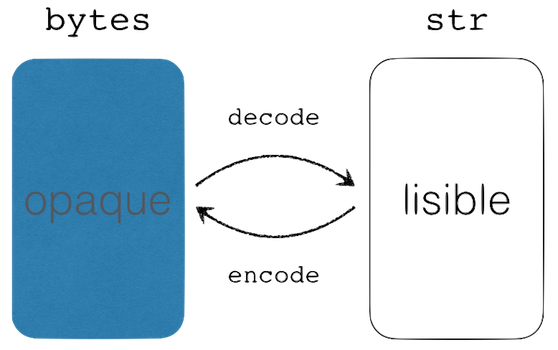
\includegraphics{medias/str-bytes.png}
\caption{les types bytes et str}
\end{figure}

    On peut appeler les méthodes \texttt{encode} et \texttt{decode} sans
préciser l'encodage (dans ce cas Python choisit l'encodage par défaut
sur votre système). Cela dit, il est de loin préférable d'être explicite
et de choisir son encodage. En cas de doute, il est recommandé de
\textbf{spécifier explicitement} \texttt{utf-8}, qui se généralise au
détriment d'encodages anciens comme \texttt{cp1242} (Windows) et
\texttt{iso8859-*}, que de laisser le système hôte choisir pour vous.

    \hypertarget{utilisation-des-accents-et-autres-cuxe9dilles}{%
\subparagraph{Utilisation des accents et autres
cédilles\\\\}\label{utilisation-des-accents-et-autres-cuxe9dilles}}

    Python 3 supporte Unicode par défaut. Vous pouvez donc, maintenant,
utiliser sans aucun risque des accents ou des cédilles dans vos chaînes
de caractères. Il faut cependant faire attention à deux choses~:

\begin{itemize}
	\item
	Python supporte Unicode, donc tous les caractères du monde, mais les
	ordinateurs n'ont pas forcément les polices de caractères nécessaires
	pour afficher ces caractères~;
	\item
	Python permet d'utiliser des caractères
	Unicode pour les noms de variables, mais nous vous recommandons dans
	toute la mesure du possible d'écrire votre code en anglais, comme c'est
	le cas pour la quasi-totalité du code que vous serez amenés à utiliser
	sous forme de bibliothèques.
\end{itemize}

Ainsi, il faut bien distinguer les chaînes de caractères qui doivent par
nature être adaptées au langage des utilisateurs du programme, et le
code source qui lui est destiné aux programmeurs et qui doit donc éviter
d'utiliser autre chose que de l'anglais.

    \hypertarget{compluxe9ment---niveau-intermuxe9diaire}{%
\subsection{Complément - niveau
intermédiaire}\label{compluxe9ment---niveau-intermuxe9diaire}}

    \hypertarget{ouxf9-peut-on-mettre-des-accents}{%
\subsubsection{Où peut-on mettre des
accents~?}\label{ouxf9-peut-on-mettre-des-accents}}

    Cela étant dit, si vous devez vraiment mettre des accents dans vos
sources, voici ce qu'il faut savoir.

    \hypertarget{noms-de-variables}{%
\paragraph{Noms de variables}\label{noms-de-variables}}

    \begin{itemize}
\tightlist
\item
  S'il n'était \textbf{pas possible en Python 2} d'utiliser un caractère
  accentué dans un \textbf{nom de variable} (ou d'un identificateur au
  sens large), cela est à présent \textbf{permis en Python 3}~:
\end{itemize}

    \begin{Verbatim}[commandchars=\\\{\}]
{\color{incolor}In [{\color{incolor}1}]:} \PY{c+c1}{\PYZsh{} pas recommandé, mais autorisé par le langage}
        \PY{n}{nb\PYZus{}élèves} \PY{o}{=} \PY{l+m+mi}{12}
\end{Verbatim}


    \begin{itemize}
\tightlist
\item
  On peut même utiliser des symboles, comme par exemple
\end{itemize}

    \begin{Verbatim}[commandchars=\\\{\}]
{\color{incolor}In [{\color{incolor}2}]:} \PY{k+kn}{from} \PY{n+nn}{math} \PY{k}{import} \PY{n}{cos}\PY{p}{,} \PY{n}{pi} \PY{k}{as} \PY{n}{Π}
        \PY{n}{θ} \PY{o}{=} \PY{n}{Π} \PY{o}{/} \PY{l+m+mi}{4}
        \PY{n}{cos}\PY{p}{(}\PY{n}{θ}\PY{p}{)}
\end{Verbatim}


\begin{Verbatim}[commandchars=\\\{\}]
{\color{outcolor}Out[{\color{outcolor}2}]:} 0.7071067811865476
\end{Verbatim}
            
\begin{itemize}
\tightlist
\item
  Je vous recommande toutefois de \textbf{ne pas utiliser} cette
  possibilité, si vous n'êtes pas extrêmement familier avec les
  caractères Unicode.
\end{itemize}

    \begin{itemize}
\tightlist
\item
  Enfin, pour être exhaustif, sachez que seule une partie des caractères
  Unicode sont autorisés dans ce cadre, c'est heureux parce que les
  caractères comme, par exemple,
  \href{http://www.fileformat.info/info/unicode/char/a0/index.htm}{l'espace
  non-sécable} pourraient, s'ils étaient autorisés, être la cause de
  milliers d'heures de debugging à frustration garantie :)
\end{itemize}

Pour les curieux, vous pouvez en savoir plus
\href{https://docs.python.org/3/reference/lexical_analysis.html\#identifiers}{à
cet endroit de la documentation officielle (en anglais)}.

    \hypertarget{chauxeenes-de-caractuxe8res}{%
\paragraph{Chaînes de caractères}\label{chauxeenes-de-caractuxe8res}}

    \begin{itemize}
\item
  Vous pouvez naturellement mettre des accents dans les chaînes de
  caractères. Cela dit, les données manipulées par un programme
  proviennent pour l'essentiel de sources externes, comme une base de
  données ou un formulaire Web, et donc le plus souvent pas directement
  du code source. Les chaînes de caractères présentes dans du vrai code
  sont bien souvent limitées à des messages de logging, et le plus
  souvent d'ailleurs en anglais, donc sans accent.
\item
  Lorsque votre programme doit interagir avec les utilisateurs et qu'il
  doit donc parler leur langue, c'est une bonne pratique de créer un
  fichier spécifique, que l'on appelle fichier de ressources, qui
  contient toutes les chaînes de caractères spécifiques à une langue.
  Ainsi, la traduction de votre programme consistera à simplement
  traduire ce fichier de ressources.
\end{itemize}

    \begin{Shaded}
\begin{Highlighting}[]
\NormalTok{message }\OperatorTok{=} \StringTok{"on peut mettre un caractère accentué dans une chaîne"}
\end{Highlighting}
\end{Shaded}

    \hypertarget{commentaires}{%
\paragraph{Commentaires}\label{commentaires}}

    \begin{itemize}
\tightlist
\item
  Enfin on peut aussi bien sûr mettre dans les commentaires n'importe
  quel caractère Unicode, et donc notamment des caractères accentués si
  on choisit malgré tout d'écrire le code en français.
\end{itemize}

    \begin{Shaded}
\begin{Highlighting}[]
\CommentTok{# on peut mettre un caractère accentué dans un commentaire}
\CommentTok{# ainsi que cos(Θ)  \(\forall x \in \int\)f(t)dt \(\iiint\) vous voyez l'idée générale}
\end{Highlighting}
\end{Shaded}

    \hypertarget{quest-ce-quun-encodage}{%
\subsubsection{Qu'est-ce qu'un
encodage~?}\label{quest-ce-quun-encodage}}

    Comme vous le savez, la mémoire - ou le disque - d'un ordinateur ne
permet que de stocker des représentations binaires. Il n'y a donc pas de
façon ``naturelle'' de représenter un caractère comme `A', un guillemet
ou un point-virgule.\\

On utilise pour cela un encodage, par exemple le code \texttt{US-ASCII}
- \href{http://www.asciitable.com/}{http://www.asciitable.com/} - stipule, pour faire simple, qu'un `A' est
représenté par l'octet 65 qui s'écrit en binaire 01000001. Il se trouve
qu'il existe plusieurs encodages, bien sûr incompatibles, selon les
systèmes et les langues. Vous trouverez plus de détails ci-dessous.\\

Le point important est que pour pouvoir ouvrir un fichier
``proprement'', il faut bien entendu disposer du \textbf{contenu} du
fichier, mais il faut aussi connaître l'\textbf{encodage} qui a été
utilisé pour l'écrire.

    \hypertarget{pruxe9cautions-uxe0-prendre-pour-lencodage-de-votre-code-source}{%
\subsubsection{Précautions à prendre pour l'encodage de votre code
source}\label{pruxe9cautions-uxe0-prendre-pour-lencodage-de-votre-code-source}}

    L'encodage ne concerne pas simplement les objets chaîne de caractères,
mais également votre code source. \textbf{Python 3} considère que votre
code source utilise \textbf{par défaut l'encodage \texttt{UTF-8}}. Nous
vous conseillons de conserver cet encodage qui est celui qui vous
offrira le plus de flexibilité.\\

    Vous pouvez malgré tout changer l'encodage \textbf{de votre code source}
en faisant figurer dans vos fichiers, \textbf{en première ou deuxième
ligne}, une déclaration comme ceci~:

\begin{Shaded}
\begin{Highlighting}[]
\CommentTok{# -*- coding: <nom_de_l_encodage> -*-}
\end{Highlighting}
\end{Shaded}

ou plus simplement, comme ceci~:

\begin{Shaded}
\begin{Highlighting}[]
\CommentTok{# coding: <nom_de_l_encodage>}
\end{Highlighting}
\end{Shaded}

Notons que la première option est également interprétée par l'éditeur de
texte \emph{Emacs} pour utiliser le même encodage. En dehors de
l'utilisation d'Emacs, la deuxième option, plus simple et donc plus
pythonique, est à préférer.\\

    Le nom \textbf{\texttt{UTF-8}} fait référence à \textbf{Unicode} (ou
pour être précis, à l'encodage le plus répandu parmi ceux qui sont
définis dans la norme Unicode, comme nous le verrons plus bas). Sur
certains systèmes plus anciens vous pourrez être amenés à utiliser un
autre encodage. Pour déterminer la valeur à utiliser dans votre cas
précis vous pouvez faire dans l'interpréteur interactif~:

    \begin{Shaded}
\begin{Highlighting}[]
\CommentTok{# ceci doit être exécuté sur votre machine}
\ImportTok{import}\NormalTok{ sys}
\BuiltInTok{print}\NormalTok{(sys.getdefaultencoding())}
\end{Highlighting}
\end{Shaded}

    Par exemple avec d'anciennes versions de Windows (en principe de plus en
plus rares) vous pouvez être amenés à écrire~:

    \begin{Shaded}
\begin{Highlighting}[]
\CommentTok{# coding: cp1252}
\end{Highlighting}
\end{Shaded}

    La syntaxe de la ligne \texttt{coding} est précisée dans
\href{https://docs.python.org/3/reference/lexical_analysis.html\#encoding-declarations}{cette
documentation} et dans le
\href{https://www.python.org/dev/peps/pep-0263/}{PEP 263}.

    \hypertarget{le-grand-malentendu}{%
\subsubsection{Le grand malentendu}\label{le-grand-malentendu}}

    Si je vous envoie un fichier contenant du français encodé avec, disons,
\texttt{ISO/IEC\ 8859-15} (\texttt{Latin-9}) --
\href{http://en.wikipedia.org/wiki/ISO/IEC\_8859-15}{http://en.wikipedia.org/wiki/ISO/IEC\_8859-15} -- vous pouvez voir dans
la table qu'un caractère `€' va être matérialisé dans mon fichier par un
octet `0xA4', soit 164.\\

Imaginez maintenant que vous essayez d'ouvrir ce même fichier depuis un
vieil ordinateur Windows configuré pour le français. Si on ne lui donne
aucune indication sur l'encodage, le programme qui va lire ce fichier
sur Windows va utiliser l'encodage par défaut du système, c'est-à-dire
\texttt{CP1252} -- \href{http://en.wikipedia.org/wiki/Windows-1252}{http://en.wikipedia.org/wiki/Windows-1252}. Comme vous
le voyez dans cette table, l'octet `0xA4' correspond au caractère ¤ et
c'est ça que vous allez voir à la place de €.\\

C'est à cela que sert la balise
\texttt{\#\ coding:\ \textless{}nom\_de\_l\_encodage\textgreater{}}.\\

De cette manière, Python lorsqu'il lit votre code source, a les moyens
d'interpréter correctement son contenu car il sait quel encodage
utiliser. On vous rappelle que si vous ne spécifiez aucun encodage pour
votre code source, Python utilisera l'encodage \texttt{UTF-8}, ce qui
est souvent le meilleur choix.

    \hypertarget{pourquoi-uxe7a-marche-en-local}{%
\subsubsection{Pourquoi ça marche en
local~?}\label{pourquoi-uxe7a-marche-en-local}}

    Lorsque le producteur (le programme qui écrit le fichier) et le
consommateur (le programme qui le lit) tournent dans le même ordinateur,
tout fonctionne bien - en général - parce que les deux programmes se
ramènent à l'encodage défini comme l'encodage par défaut. On a vu
pourquoi il vaut mieux toutefois être explicite, et spécifier la balise
\texttt{\#\ coding:\ ...}\\

Il y a toutefois une limite, si vous utilisez un Linux configuré de
manière minimale, il se peut qu'il utilise par défaut l'encodage
\texttt{US-ASCII} - voir plus bas - qui étant très ancien ne ``connaît''
pas un simple é, ni a fortiori €. Pour écrire du français, il faut donc
au minimum que l'encodage par défaut de votre ordinateur contienne les
caractères français, comme par exemple~:
\begin{itemize}
	\item
	\texttt{ISO\ 8859-1} (\texttt{Latin-1})
	\item
	\texttt{ISO\ 8859-15} (\texttt{Latin-9})
	\item
	\texttt{UTF-8}
	\item
	\texttt{CP1252}
\end{itemize}

    \hypertarget{un-peu-dhistoire-sur-les-encodages}{%
\subsubsection{Un peu d'histoire sur les
encodages}\label{un-peu-dhistoire-sur-les-encodages}}

    \hypertarget{le-code-us-ascii}{%
\subparagraph{\texorpdfstring{Le code
\texttt{US-ASCII}}{Le code US-ASCII}\\\\}\label{le-code-us-ascii}}

    Jusque dans les années 1980, les ordinateurs ne parlaient pour
l'essentiel que l'anglais. La première vague de standardisation avait
créé l'encodage dit \texttt{ASCII}, ou encore \texttt{US-ASCII} - voir
par exemple \href{http://www.asciitable.com}{http://www.asciitable.com}, ou en version longue
\href{http://en.wikipedia.org/wiki/ASCII}{http://en.wikipedia.org/wiki/ASCII}.\\

Le code \texttt{US-ASCII} s'étend sur 128 valeurs, soit 7 bits, mais est
le plus souvent implémenté sur un octet pour préserver l'alignement, le
dernier bit pouvant être utilisé par exemple pour ajouter un code
correcteur d'erreur - ce qui à l'époque des modems n'était pas superflu.
Bref, la pratique courante était alors de manipuler une chaîne de
caractères comme un tableau d'octets.

    \hypertarget{les-encodages-iso8859--latin}{%
\subparagraph{\texorpdfstring{Les encodages \texttt{ISO8859-*}
(\texttt{Latin*})}{Les encodages ISO8859-* (Latin*)}\\\\}\label{les-encodages-iso8859--latin}}

    Dans les années 1990, pour satisfaire les besoins des pays européens,
ont été définis plusieurs encodages alternatifs, connus sous le nom de
\href{http://en.wikipedia.org/wiki/ISO/IEC_8859}{\texttt{ISO/IEC\ 8859-*}},
nommés aussi \texttt{Latin-*}. Idéalement, on aurait pu et
\textbf{certainement dû} définir un seul encodage pour représenter tous
les nouveaux caractères, mais entre toutes les langues européennes, le
nombre de caractères à ajouter était substantiel, et cet encodage unifié
aurait largement dépassé 256 caractères différents, il n'aurait donc
\textbf{pas été possible} de tout faire tenir sur un octet.\\

On a préféré préserver la ``bonne propriété'' du modèle \emph{un
caractère} == \emph{un octet}, ceci afin de préserver le code existant
qui aurait sinon dû être retouché ou réécrit.\\

Dès lors il n'y avait pas d'autre choix que de définir
\textbf{plusieurs} encodages distincts, par exemple, pour le français on
a utilisé à l'époque
\href{http://en.wikipedia.org/wiki/ISO/IEC_8859-1}{\texttt{ISO/IEC\ 8859-1}
(\texttt{Latin-1})}, pour le russe
\href{http://en.wikipedia.org/wiki/ISO/IEC_8859-5}{\texttt{ISO/IEC\ 5589-5}
(\texttt{Latin/Cyrillic})}.\\

À ce stade, le ver était dans le fruit. Depuis cette époque pour ouvrir
un fichier il faut connaître son encodage.

    \hypertarget{unicode}{%
\subparagraph{Unicode\\\\}\label{unicode}}

    Lorsque l'on a ensuite cherché à manipuler aussi les langues asiatiques,
il a de toute façon fallu définir de nouveaux encodages beaucoup plus
larges. C'est ce qui a été fait par le standard
\href{http://en.wikipedia.org/wiki/Unicode}{Unicode} qui définit 3
nouveaux encodages~:
\begin{itemize}
	\item
	\href{http://en.wikipedia.org/wiki/UTF-8}{\texttt{UTF-8}} : un encodage
	à taille variable, à base d'octets, qui maximise la compatibilité avec
	US-ASCII~;
	\item
	\href{http://en.wikipedia.org/wiki/UTF-16}{\texttt{UTF-16}}
	: un encodage à taille variable, à base de mots de 16 bits~;
	\item
	\href{http://en.wikipedia.org/wiki/UTF-32}{\texttt{UTF-32}} : un
	encodage à taille fixe, à base de mots de 32 bits~;\\
\end{itemize}
Ces 3 standards couvrent le même jeu de caractères (113 021 tout de même
dans la dernière version). Parmi ceux-ci le plus utilisé est
certainement \texttt{UTF-8}. Un texte ne contenant que des caractères du
code \texttt{US-ASCII} initial peut être lu avec l'encodage
\texttt{UTF-8}.\\

Pour être enfin tout à fait exhaustif, si on sait qu'un fichier est au
format Unicode, on peut déterminer quel est l'encodage qu'il utilise, en
se basant sur les 4 premiers octets du document. Ainsi dans ce cas
particulier (lorsqu'on est sûr qu'un document utilise un des trois
encodages Unicode) il n'est plus nécessaire de connaître son encodage de
manière ``externe''.    
        \hypertarget{les-outils-de-base-sur-les-chauxeenes-de-caractuxe8res-str}{%
\section{\texorpdfstring{Les outils de base sur les chaînes de
caractères
(\texttt{str})}{Les outils de base sur les chaînes de caractères (str)}}\label{les-outils-de-base-sur-les-chauxeenes-de-caractuxe8res-str}}

    \hypertarget{compluxe9ment---niveau-intermuxe9diaire}{%
\subsection{Complément - niveau
intermédiaire}\label{compluxe9ment---niveau-intermuxe9diaire}}

    \hypertarget{lire-la-documentation}{%
\subsubsection{Lire la documentation}\label{lire-la-documentation}}

    Même après des années de pratique, il est difficile de se souvenir de
toutes les méthodes travaillant sur les chaînes de caractères. Aussi il
est toujours utile de recourir à la documentation embarquée

    \begin{Verbatim}[commandchars=\\\{\}]
{\color{incolor}In [{\color{incolor}1}]:} \PY{n}{help}\PY{p}{(}\PY{n+nb}{str}\PY{p}{)}
\end{Verbatim}



    Nous allons tenter ici de citer les méthodes les plus utilisées. Nous
n'avons le temps que de les utiliser de manière très simple, mais bien
souvent il est possible de passer en argument des options permettant de
ne travailler que sur une sous-chaîne, ou sur la première ou dernière
occurrence d'une sous-chaîne. Nous vous renvoyons à la documentation
pour obtenir toutes les précisions utiles.

    \hypertarget{duxe9coupage---assemblage-split-et-join}{%
\subsubsection{\texorpdfstring{Découpage - assemblage~: \texttt{split}
et
\texttt{join}}{Découpage - assemblage~: split et join}}\label{duxe9coupage---assemblage-split-et-join}}

    Les méthodes \texttt{split} et \texttt{join} permettent de découper une
chaîne selon un séparateur pour obtenir une liste, et à l'inverse de
reconstruire une chaîne à partir d'une liste.

    \texttt{split} permet donc de découper~:

    \begin{Verbatim}[commandchars=\\\{\}]
{\color{incolor}In [{\color{incolor}2}]:} \PY{l+s+s1}{\PYZsq{}}\PY{l+s+s1}{abc=:=def=:=ghi=:=jkl}\PY{l+s+s1}{\PYZsq{}}\PY{o}{.}\PY{n}{split}\PY{p}{(}\PY{l+s+s1}{\PYZsq{}}\PY{l+s+s1}{=:=}\PY{l+s+s1}{\PYZsq{}}\PY{p}{)}
\end{Verbatim}


\begin{Verbatim}[commandchars=\\\{\}]
{\color{outcolor}Out[{\color{outcolor}2}]:} ['abc', 'def', 'ghi', 'jkl']
\end{Verbatim}
            
    Et à l'inverse~:

    \begin{Verbatim}[commandchars=\\\{\}]
{\color{incolor}In [{\color{incolor}3}]:} \PY{l+s+s2}{\PYZdq{}}\PY{l+s+s2}{=:=}\PY{l+s+s2}{\PYZdq{}}\PY{o}{.}\PY{n}{join}\PY{p}{(}\PY{p}{[}\PY{l+s+s1}{\PYZsq{}}\PY{l+s+s1}{abc}\PY{l+s+s1}{\PYZsq{}}\PY{p}{,} \PY{l+s+s1}{\PYZsq{}}\PY{l+s+s1}{def}\PY{l+s+s1}{\PYZsq{}}\PY{p}{,} \PY{l+s+s1}{\PYZsq{}}\PY{l+s+s1}{ghi}\PY{l+s+s1}{\PYZsq{}}\PY{p}{,} \PY{l+s+s1}{\PYZsq{}}\PY{l+s+s1}{jkl}\PY{l+s+s1}{\PYZsq{}}\PY{p}{]}\PY{p}{)}
\end{Verbatim}


\begin{Verbatim}[commandchars=\\\{\}]
{\color{outcolor}Out[{\color{outcolor}3}]:} 'abc=:=def=:=ghi=:=jkl'
\end{Verbatim}
            
    Attention toutefois si le séparateur est un terminateur, la liste
résultat contient alors une dernière chaîne vide. En pratique, on
utilisera la méthode \texttt{strip}, que nous allons voir ci-dessous,
avant la méthode \texttt{split} pour éviter ce problème.

    \begin{Verbatim}[commandchars=\\\{\}]
{\color{incolor}In [{\color{incolor}4}]:} \PY{l+s+s1}{\PYZsq{}}\PY{l+s+s1}{abc;def;ghi;jkl;}\PY{l+s+s1}{\PYZsq{}}\PY{o}{.}\PY{n}{split}\PY{p}{(}\PY{l+s+s1}{\PYZsq{}}\PY{l+s+s1}{;}\PY{l+s+s1}{\PYZsq{}}\PY{p}{)}
\end{Verbatim}


\begin{Verbatim}[commandchars=\\\{\}]
{\color{outcolor}Out[{\color{outcolor}4}]:} ['abc', 'def', 'ghi', 'jkl', '']
\end{Verbatim}
            
    Qui s'inverse correctement cependant~:

    \begin{Verbatim}[commandchars=\\\{\}]
{\color{incolor}In [{\color{incolor}5}]:} \PY{l+s+s2}{\PYZdq{}}\PY{l+s+s2}{;}\PY{l+s+s2}{\PYZdq{}}\PY{o}{.}\PY{n}{join}\PY{p}{(}\PY{p}{[}\PY{l+s+s1}{\PYZsq{}}\PY{l+s+s1}{abc}\PY{l+s+s1}{\PYZsq{}}\PY{p}{,} \PY{l+s+s1}{\PYZsq{}}\PY{l+s+s1}{def}\PY{l+s+s1}{\PYZsq{}}\PY{p}{,} \PY{l+s+s1}{\PYZsq{}}\PY{l+s+s1}{ghi}\PY{l+s+s1}{\PYZsq{}}\PY{p}{,} \PY{l+s+s1}{\PYZsq{}}\PY{l+s+s1}{jkl}\PY{l+s+s1}{\PYZsq{}}\PY{p}{,} \PY{l+s+s1}{\PYZsq{}}\PY{l+s+s1}{\PYZsq{}}\PY{p}{]}\PY{p}{)}
\end{Verbatim}


\begin{Verbatim}[commandchars=\\\{\}]
{\color{outcolor}Out[{\color{outcolor}5}]:} 'abc;def;ghi;jkl;'
\end{Verbatim}
            
    \hypertarget{remplacement-replace}{%
\subsubsection{\texorpdfstring{Remplacement~:
\texttt{replace}}{Remplacement~: replace}}\label{remplacement-replace}}

    \texttt{replace} est très pratique pour remplacer une sous-chaîne par
une autre, avec une limite éventuelle sur le nombre de remplacements~:

    \begin{Verbatim}[commandchars=\\\{\}]
{\color{incolor}In [{\color{incolor}6}]:} \PY{l+s+s2}{\PYZdq{}}\PY{l+s+s2}{abcdefabcdefabcdef}\PY{l+s+s2}{\PYZdq{}}\PY{o}{.}\PY{n}{replace}\PY{p}{(}\PY{l+s+s2}{\PYZdq{}}\PY{l+s+s2}{abc}\PY{l+s+s2}{\PYZdq{}}\PY{p}{,} \PY{l+s+s2}{\PYZdq{}}\PY{l+s+s2}{zoo}\PY{l+s+s2}{\PYZdq{}}\PY{p}{)}
\end{Verbatim}


\begin{Verbatim}[commandchars=\\\{\}]
{\color{outcolor}Out[{\color{outcolor}6}]:} 'zoodefzoodefzoodef'
\end{Verbatim}
            
    \begin{Verbatim}[commandchars=\\\{\}]
{\color{incolor}In [{\color{incolor}7}]:} \PY{l+s+s2}{\PYZdq{}}\PY{l+s+s2}{abcdefabcdefabcdef}\PY{l+s+s2}{\PYZdq{}}\PY{o}{.}\PY{n}{replace}\PY{p}{(}\PY{l+s+s2}{\PYZdq{}}\PY{l+s+s2}{abc}\PY{l+s+s2}{\PYZdq{}}\PY{p}{,} \PY{l+s+s2}{\PYZdq{}}\PY{l+s+s2}{zoo}\PY{l+s+s2}{\PYZdq{}}\PY{p}{,} \PY{l+m+mi}{2}\PY{p}{)}
\end{Verbatim}


\begin{Verbatim}[commandchars=\\\{\}]
{\color{outcolor}Out[{\color{outcolor}7}]:} 'zoodefzoodefabcdef'
\end{Verbatim}
            
    Plusieurs appels à \texttt{replace} peuvent être chaînés comme ceci~:

    \begin{Verbatim}[commandchars=\\\{\}]
{\color{incolor}In [{\color{incolor}8}]:} \PY{l+s+s2}{\PYZdq{}}\PY{l+s+s2}{les [x] qui disent [y]}\PY{l+s+s2}{\PYZdq{}}\PY{o}{.}\PY{n}{replace}\PY{p}{(}\PY{l+s+s2}{\PYZdq{}}\PY{l+s+s2}{[x]}\PY{l+s+s2}{\PYZdq{}}\PY{p}{,} \PY{l+s+s2}{\PYZdq{}}\PY{l+s+s2}{chevaliers}\PY{l+s+s2}{\PYZdq{}}\PY{p}{)}\PY{o}{.}\PY{n}{replace}\PY{p}{(}\PY{l+s+s2}{\PYZdq{}}\PY{l+s+s2}{[y]}\PY{l+s+s2}{\PYZdq{}}\PY{p}{,} \PY{l+s+s2}{\PYZdq{}}\PY{l+s+s2}{Ni}\PY{l+s+s2}{\PYZdq{}}\PY{p}{)}
\end{Verbatim}


\begin{Verbatim}[commandchars=\\\{\}]
{\color{outcolor}Out[{\color{outcolor}8}]:} 'les chevaliers qui disent Ni'
\end{Verbatim}
            
    \hypertarget{nettoyage-strip}{%
\subsubsection{\texorpdfstring{Nettoyage~:
\texttt{strip}}{Nettoyage~: strip}}\label{nettoyage-strip}}

    On pourrait par exemple utiliser \texttt{replace} pour enlever les
espaces dans une chaîne, ce qui peut être utile pour ``nettoyer'' comme
ceci~:

    \begin{Verbatim}[commandchars=\\\{\}]
{\color{incolor}In [{\color{incolor}9}]:} \PY{l+s+s2}{\PYZdq{}}\PY{l+s+s2}{ abc:def:ghi }\PY{l+s+s2}{\PYZdq{}}\PY{o}{.}\PY{n}{replace}\PY{p}{(}\PY{l+s+s2}{\PYZdq{}}\PY{l+s+s2}{ }\PY{l+s+s2}{\PYZdq{}}\PY{p}{,} \PY{l+s+s2}{\PYZdq{}}\PY{l+s+s2}{\PYZdq{}}\PY{p}{)}
\end{Verbatim}


\begin{Verbatim}[commandchars=\\\{\}]
{\color{outcolor}Out[{\color{outcolor}9}]:} 'abc:def:ghi'
\end{Verbatim}
            
    Toutefois bien souvent on préfère utiliser \texttt{strip} qui ne
s'occupe que du début et de la fin de la chaîne, et gère aussi les
tabulations et autres retour à la ligne~:

    \begin{Verbatim}[commandchars=\\\{\}]
{\color{incolor}In [{\color{incolor}10}]:} \PY{l+s+s2}{\PYZdq{}}\PY{l+s+s2}{ }\PY{l+s+se}{\PYZbs{}t}\PY{l+s+s2}{une chaîne avec des trucs qui dépassent }\PY{l+s+se}{\PYZbs{}n}\PY{l+s+s2}{\PYZdq{}}\PY{o}{.}\PY{n}{strip}\PY{p}{(}\PY{p}{)}
\end{Verbatim}


\begin{Verbatim}[commandchars=\\\{\}]
{\color{outcolor}Out[{\color{outcolor}10}]:} 'une chaîne avec des trucs qui dépassent'
\end{Verbatim}
            
    On peut appliquer \texttt{strip} avant \texttt{split} pour éviter le
problème du dernier élément vide~:

    \begin{Verbatim}[commandchars=\\\{\}]
{\color{incolor}In [{\color{incolor}11}]:} \PY{l+s+s1}{\PYZsq{}}\PY{l+s+s1}{abc;def;ghi;jkl;}\PY{l+s+s1}{\PYZsq{}}\PY{o}{.}\PY{n}{strip}\PY{p}{(}\PY{l+s+s1}{\PYZsq{}}\PY{l+s+s1}{;}\PY{l+s+s1}{\PYZsq{}}\PY{p}{)}\PY{o}{.}\PY{n}{split}\PY{p}{(}\PY{l+s+s1}{\PYZsq{}}\PY{l+s+s1}{;}\PY{l+s+s1}{\PYZsq{}}\PY{p}{)}
\end{Verbatim}


\begin{Verbatim}[commandchars=\\\{\}]
{\color{outcolor}Out[{\color{outcolor}11}]:} ['abc', 'def', 'ghi', 'jkl']
\end{Verbatim}
            
    \hypertarget{rechercher-une-sous-chauxeene}{%
\subsubsection{Rechercher une
sous-chaîne}\label{rechercher-une-sous-chauxeene}}

    Plusieurs outils permettent de chercher une sous-chaîne. Il existe
\texttt{find} qui renvoie le plus petit index où on trouve la
sous-chaîne~:

    \begin{Verbatim}[commandchars=\\\{\}]
{\color{incolor}In [{\color{incolor}12}]:} \PY{c+c1}{\PYZsh{} l\PYZsq{}indice du début de la première occurrence}
         \PY{l+s+s2}{\PYZdq{}}\PY{l+s+s2}{abcdefcdefghefghijk}\PY{l+s+s2}{\PYZdq{}}\PY{o}{.}\PY{n}{find}\PY{p}{(}\PY{l+s+s2}{\PYZdq{}}\PY{l+s+s2}{def}\PY{l+s+s2}{\PYZdq{}}\PY{p}{)}
\end{Verbatim}


\begin{Verbatim}[commandchars=\\\{\}]
{\color{outcolor}Out[{\color{outcolor}12}]:} 3
\end{Verbatim}
            
    \begin{Verbatim}[commandchars=\\\{\}]
{\color{incolor}In [{\color{incolor}13}]:} \PY{c+c1}{\PYZsh{} ou \PYZhy{}1 si la chaîne n\PYZsq{}est pas présente}
         \PY{l+s+s2}{\PYZdq{}}\PY{l+s+s2}{abcdefcdefghefghijk}\PY{l+s+s2}{\PYZdq{}}\PY{o}{.}\PY{n}{find}\PY{p}{(}\PY{l+s+s2}{\PYZdq{}}\PY{l+s+s2}{zoo}\PY{l+s+s2}{\PYZdq{}}\PY{p}{)}
\end{Verbatim}


\begin{Verbatim}[commandchars=\\\{\}]
{\color{outcolor}Out[{\color{outcolor}13}]:} -1
\end{Verbatim}
            
    \texttt{rfind} fonctionne comme \texttt{find} mais en partant de la fin
de la chaîne~:

    \begin{Verbatim}[commandchars=\\\{\}]
{\color{incolor}In [{\color{incolor}14}]:} \PY{c+c1}{\PYZsh{} en partant de la fin}
         \PY{l+s+s2}{\PYZdq{}}\PY{l+s+s2}{abcdefcdefghefghijk}\PY{l+s+s2}{\PYZdq{}}\PY{o}{.}\PY{n}{rfind}\PY{p}{(}\PY{l+s+s2}{\PYZdq{}}\PY{l+s+s2}{fgh}\PY{l+s+s2}{\PYZdq{}}\PY{p}{)}
\end{Verbatim}


\begin{Verbatim}[commandchars=\\\{\}]
{\color{outcolor}Out[{\color{outcolor}14}]:} 13
\end{Verbatim}
            
    \begin{Verbatim}[commandchars=\\\{\}]
{\color{incolor}In [{\color{incolor}15}]:} \PY{c+c1}{\PYZsh{} notez que le résultat correspond}
         \PY{c+c1}{\PYZsh{} tout de même toujours au début de la chaîne}
         \PY{l+s+s2}{\PYZdq{}}\PY{l+s+s2}{abcdefcdefghefghijk}\PY{l+s+s2}{\PYZdq{}}\PY{p}{[}\PY{l+m+mi}{13}\PY{p}{]}
\end{Verbatim}


\begin{Verbatim}[commandchars=\\\{\}]
{\color{outcolor}Out[{\color{outcolor}15}]:} 'f'
\end{Verbatim}
            
    La méthode \texttt{index} se comporte comme \texttt{find}, mais en cas
d'absence elle lève une \textbf{exception} (nous verrons ce concept plus
tard) plutôt que de renvoyer \texttt{-1}~:

    \begin{Verbatim}[commandchars=\\\{\}]
{\color{incolor}In [{\color{incolor}16}]:} \PY{l+s+s2}{\PYZdq{}}\PY{l+s+s2}{abcdefcdefghefghijk}\PY{l+s+s2}{\PYZdq{}}\PY{o}{.}\PY{n}{index}\PY{p}{(}\PY{l+s+s2}{\PYZdq{}}\PY{l+s+s2}{def}\PY{l+s+s2}{\PYZdq{}}\PY{p}{)}
\end{Verbatim}


\begin{Verbatim}[commandchars=\\\{\}]
{\color{outcolor}Out[{\color{outcolor}16}]:} 3
\end{Verbatim}
            
    \begin{Verbatim}[commandchars=\\\{\}]
{\color{incolor}In [{\color{incolor}17}]:} \PY{k}{try}\PY{p}{:}
             \PY{l+s+s2}{\PYZdq{}}\PY{l+s+s2}{abcdefcdefghefghijk}\PY{l+s+s2}{\PYZdq{}}\PY{o}{.}\PY{n}{index}\PY{p}{(}\PY{l+s+s2}{\PYZdq{}}\PY{l+s+s2}{zoo}\PY{l+s+s2}{\PYZdq{}}\PY{p}{)}
         \PY{k}{except} \PY{n+ne}{Exception} \PY{k}{as} \PY{n}{e}\PY{p}{:}
             \PY{n+nb}{print}\PY{p}{(}\PY{l+s+s2}{\PYZdq{}}\PY{l+s+s2}{OOPS}\PY{l+s+s2}{\PYZdq{}}\PY{p}{,} \PY{n+nb}{type}\PY{p}{(}\PY{n}{e}\PY{p}{)}\PY{p}{,} \PY{n}{e}\PY{p}{)}
\end{Verbatim}


    \begin{Verbatim}[commandchars=\\\{\}]
OOPS <class 'ValueError'> substring not found

    \end{Verbatim}

    Mais le plus simple pour chercher si une sous-chaîne est dans une autre
chaîne est d'utiliser l'instruction \texttt{in} sur laquelle nous
reviendrons lorsque nous parlerons des séquences~:

    \begin{Verbatim}[commandchars=\\\{\}]
{\color{incolor}In [{\color{incolor}18}]:} \PY{l+s+s2}{\PYZdq{}}\PY{l+s+s2}{def}\PY{l+s+s2}{\PYZdq{}} \PY{o+ow}{in} \PY{l+s+s2}{\PYZdq{}}\PY{l+s+s2}{abcdefcdefghefghijk}\PY{l+s+s2}{\PYZdq{}}
\end{Verbatim}


\begin{Verbatim}[commandchars=\\\{\}]
{\color{outcolor}Out[{\color{outcolor}18}]:} True
\end{Verbatim}
            
    La méthode \texttt{count} compte le nombre d'occurrences d'une
sous-chaîne~:

    \begin{Verbatim}[commandchars=\\\{\}]
{\color{incolor}In [{\color{incolor}19}]:} \PY{l+s+s2}{\PYZdq{}}\PY{l+s+s2}{abcdefcdefghefghijk}\PY{l+s+s2}{\PYZdq{}}\PY{o}{.}\PY{n}{count}\PY{p}{(}\PY{l+s+s2}{\PYZdq{}}\PY{l+s+s2}{ef}\PY{l+s+s2}{\PYZdq{}}\PY{p}{)}
\end{Verbatim}


\begin{Verbatim}[commandchars=\\\{\}]
{\color{outcolor}Out[{\color{outcolor}19}]:} 3
\end{Verbatim}
            
    Signalons enfin les méthodes de commodité suivantes~:

    \begin{Verbatim}[commandchars=\\\{\}]
{\color{incolor}In [{\color{incolor}20}]:} \PY{l+s+s2}{\PYZdq{}}\PY{l+s+s2}{abcdefcdefghefghijk}\PY{l+s+s2}{\PYZdq{}}\PY{o}{.}\PY{n}{startswith}\PY{p}{(}\PY{l+s+s2}{\PYZdq{}}\PY{l+s+s2}{abcd}\PY{l+s+s2}{\PYZdq{}}\PY{p}{)}
\end{Verbatim}


\begin{Verbatim}[commandchars=\\\{\}]
{\color{outcolor}Out[{\color{outcolor}20}]:} True
\end{Verbatim}
            
    \begin{Verbatim}[commandchars=\\\{\}]
{\color{incolor}In [{\color{incolor}21}]:} \PY{l+s+s2}{\PYZdq{}}\PY{l+s+s2}{abcdefcdefghefghijk}\PY{l+s+s2}{\PYZdq{}}\PY{o}{.}\PY{n}{endswith}\PY{p}{(}\PY{l+s+s2}{\PYZdq{}}\PY{l+s+s2}{ghijk}\PY{l+s+s2}{\PYZdq{}}\PY{p}{)}
\end{Verbatim}


\begin{Verbatim}[commandchars=\\\{\}]
{\color{outcolor}Out[{\color{outcolor}21}]:} True
\end{Verbatim}
            
    S'agissant des deux dernières, remarquons que~:\\

    \texttt{chaine.startswith(sous\_chaine)} \(\Longleftrightarrow\)
\texttt{chaine.find(sous\_chaine)\ ==\ 0}\\

\texttt{chaine.endswith(sous\_chaine)} \(\Longleftrightarrow\)
\texttt{chaine.rfind(sous\_chaine)\ ==\ (len(chaine)\ -\ len(sous\_chaine))}\\

    On remarque ici la supériorité, du point de vue de l'expressivité, des
méthodes pythoniques \texttt{startswith} et \texttt{endswith}.

    \hypertarget{changement-de-casse}{%
\subsubsection{Changement de casse}\label{changement-de-casse}}

    Voici pour conclure quelques méthodes utiles qui parlent d'elles-mêmes~:

    \begin{Verbatim}[commandchars=\\\{\}]
{\color{incolor}In [{\color{incolor}22}]:} \PY{l+s+s2}{\PYZdq{}}\PY{l+s+s2}{monty PYTHON}\PY{l+s+s2}{\PYZdq{}}\PY{o}{.}\PY{n}{upper}\PY{p}{(}\PY{p}{)}
\end{Verbatim}


\begin{Verbatim}[commandchars=\\\{\}]
{\color{outcolor}Out[{\color{outcolor}22}]:} 'MONTY PYTHON'
\end{Verbatim}
            
    \begin{Verbatim}[commandchars=\\\{\}]
{\color{incolor}In [{\color{incolor}23}]:} \PY{l+s+s2}{\PYZdq{}}\PY{l+s+s2}{monty PYTHON}\PY{l+s+s2}{\PYZdq{}}\PY{o}{.}\PY{n}{lower}\PY{p}{(}\PY{p}{)}
\end{Verbatim}


\begin{Verbatim}[commandchars=\\\{\}]
{\color{outcolor}Out[{\color{outcolor}23}]:} 'monty python'
\end{Verbatim}
            
    \begin{Verbatim}[commandchars=\\\{\}]
{\color{incolor}In [{\color{incolor}24}]:} \PY{l+s+s2}{\PYZdq{}}\PY{l+s+s2}{monty PYTHON}\PY{l+s+s2}{\PYZdq{}}\PY{o}{.}\PY{n}{swapcase}\PY{p}{(}\PY{p}{)}
\end{Verbatim}


\begin{Verbatim}[commandchars=\\\{\}]
{\color{outcolor}Out[{\color{outcolor}24}]:} 'MONTY python'
\end{Verbatim}
            
    \begin{Verbatim}[commandchars=\\\{\}]
{\color{incolor}In [{\color{incolor}25}]:} \PY{l+s+s2}{\PYZdq{}}\PY{l+s+s2}{monty PYTHON}\PY{l+s+s2}{\PYZdq{}}\PY{o}{.}\PY{n}{capitalize}\PY{p}{(}\PY{p}{)}
\end{Verbatim}


\begin{Verbatim}[commandchars=\\\{\}]
{\color{outcolor}Out[{\color{outcolor}25}]:} 'Monty python'
\end{Verbatim}
            
    \begin{Verbatim}[commandchars=\\\{\}]
{\color{incolor}In [{\color{incolor}26}]:} \PY{l+s+s2}{\PYZdq{}}\PY{l+s+s2}{monty PYTHON}\PY{l+s+s2}{\PYZdq{}}\PY{o}{.}\PY{n}{title}\PY{p}{(}\PY{p}{)}
\end{Verbatim}


\begin{Verbatim}[commandchars=\\\{\}]
{\color{outcolor}Out[{\color{outcolor}26}]:} 'Monty Python'
\end{Verbatim}
            
    \hypertarget{pour-en-savoir-plus}{%
\subsubsection{Pour en savoir plus}\label{pour-en-savoir-plus}}

    Tous ces outils sont
\href{https://docs.python.org/3/library/stdtypes.html\#string-methods}{documentés
en détail ici (en anglais)}.
        \hypertarget{formatage-de-chauxeenes-de-caractuxe8res}{%
\section{Formatage de chaînes de
caractères}\label{formatage-de-chauxeenes-de-caractuxe8res}}

    \hypertarget{compluxe9ment---niveau-basique}{%
\subsection{Complément - niveau
basique}\label{compluxe9ment---niveau-basique}}

    On désigne par formatage les outils qui permettent d'obtenir une
présentation fine des résultats, que ce soit pour améliorer la
lisibilité lorsqu'on s'adresse à des humains, ou pour respecter la
syntaxe d'un outil auquel on veut passer les données pour un traitement
ultérieur.

    \hypertarget{la-fonction-print}{%
\subsubsection{\texorpdfstring{La fonction
\texttt{print}}{La fonction print}}\label{la-fonction-print}}

    Nous avons jusqu'à maintenant presque toujours utilisé la fonction
\texttt{print} pour afficher nos résultats. Comme on l'a vu, celle-ci
réalise un formatage sommaire~: elle insère une espace entre les valeurs
qui lui sont passées.

    \begin{Verbatim}[commandchars=\\\{\}]
{\color{incolor}In [{\color{incolor}1}]:} \PY{n+nb}{print}\PY{p}{(}\PY{l+m+mi}{1}\PY{p}{,} \PY{l+s+s1}{\PYZsq{}}\PY{l+s+s1}{a}\PY{l+s+s1}{\PYZsq{}}\PY{p}{,} \PY{l+m+mi}{12} \PY{o}{+} \PY{l+m+mi}{4}\PY{n}{j}\PY{p}{)}
\end{Verbatim}


    \begin{Verbatim}[commandchars=\\\{\}]
1 a (12+4j)

    \end{Verbatim}

    La seule subtilité notable concernant \texttt{print} est que, par
défaut, elle ajoute un saut de ligne à la fin. Pour éviter ce
comportement, on peut passer à la fonction un argument \texttt{end}, qui
sera inséré \emph{au lieu} du saut de ligne. Ainsi par exemple~:

    \begin{Verbatim}[commandchars=\\\{\}]
{\color{incolor}In [{\color{incolor}2}]:} \PY{c+c1}{\PYZsh{} une première ligne}
        \PY{n+nb}{print}\PY{p}{(}\PY{l+s+s2}{\PYZdq{}}\PY{l+s+s2}{une}\PY{l+s+s2}{\PYZdq{}}\PY{p}{,} \PY{l+s+s2}{\PYZdq{}}\PY{l+s+s2}{seule}\PY{l+s+s2}{\PYZdq{}}\PY{p}{,} \PY{l+s+s2}{\PYZdq{}}\PY{l+s+s2}{ligne}\PY{l+s+s2}{\PYZdq{}}\PY{p}{)}
\end{Verbatim}


    \begin{Verbatim}[commandchars=\\\{\}]
une seule ligne

    \end{Verbatim}

    \begin{Verbatim}[commandchars=\\\{\}]
{\color{incolor}In [{\color{incolor}3}]:} \PY{c+c1}{\PYZsh{} une deuxième ligne en deux appels à print}
        \PY{n+nb}{print}\PY{p}{(}\PY{l+s+s2}{\PYZdq{}}\PY{l+s+s2}{une}\PY{l+s+s2}{\PYZdq{}}\PY{p}{,} \PY{l+s+s2}{\PYZdq{}}\PY{l+s+s2}{autre}\PY{l+s+s2}{\PYZdq{}}\PY{p}{,} \PY{n}{end}\PY{o}{=}\PY{l+s+s1}{\PYZsq{}}\PY{l+s+s1}{ }\PY{l+s+s1}{\PYZsq{}}\PY{p}{)}
        \PY{n+nb}{print}\PY{p}{(}\PY{l+s+s2}{\PYZdq{}}\PY{l+s+s2}{ligne}\PY{l+s+s2}{\PYZdq{}}\PY{p}{)}
\end{Verbatim}


    \begin{Verbatim}[commandchars=\\\{\}]
une autre ligne

    \end{Verbatim}

    Il faut remarquer aussi que \texttt{print} est capable d'imprimer
\textbf{n'importe quel objet}. Nous l'avons déjà fait avec les listes et
les tuples, voici par exemple un module~:

    \begin{Verbatim}[commandchars=\\\{\}]
{\color{incolor}In [{\color{incolor}4}]:} \PY{c+c1}{\PYZsh{} on peut imprimer par exemple un objet \PYZsq{}module\PYZsq{}}
        \PY{k+kn}{import} \PY{n+nn}{math}
        
        \PY{n+nb}{print}\PY{p}{(}\PY{l+s+s1}{\PYZsq{}}\PY{l+s+s1}{le module math est}\PY{l+s+s1}{\PYZsq{}}\PY{p}{,} \PY{n}{math}\PY{p}{)}
\end{Verbatim}


    \begin{Verbatim}[commandchars=\\\{\}]
le module math est <module 'math' (built-in)>

    \end{Verbatim}

    En anticipant un peu, voici comment \texttt{print} présente les
instances de classe (ne vous inquiétez pas, nous apprendrons dans une
semaine ultérieure ce que sont les classes et les instances).

    \begin{Verbatim}[commandchars=\\\{\}]
{\color{incolor}In [{\color{incolor}5}]:} \PY{c+c1}{\PYZsh{} pour définir la classe Personne}
        \PY{k}{class} \PY{n+nc}{Personne}\PY{p}{:}
            \PY{k}{pass}
        
        \PY{c+c1}{\PYZsh{} et pour créer une instance de cette classe}
        \PY{n}{personne} \PY{o}{=} \PY{n}{Personne}\PY{p}{(}\PY{p}{)}
\end{Verbatim}


    \begin{Verbatim}[commandchars=\\\{\}]
{\color{incolor}In [{\color{incolor}6}]:} \PY{c+c1}{\PYZsh{} voilà comment s\PYZsq{}affiche une instance de classe}
        \PY{n+nb}{print}\PY{p}{(}\PY{n}{personne}\PY{p}{)}
\end{Verbatim}


    \begin{Verbatim}[commandchars=\\\{\}]
<\_\_main\_\_.Personne object at 0x0502DB30>

    \end{Verbatim}

    On rencontre assez vite les limites de \texttt{print}~:

\begin{itemize}
\tightlist
\item
  d'une part, il peut être nécessaire de formater une chaîne de
  caractères sans nécessairement vouloir l'imprimer, ou en tout cas pas
  immédiatement~;
\item
  d'autre part, les espaces ajoutées peuvent être plus néfastes
  qu'utiles~;
\item
  enfin, on peut avoir besoin de préciser un nombre de chiffres
  significatifs, ou de choisir comment présenter une date.
\end{itemize}

C'est pourquoi il est plus courant de \textbf{formater} les chaînes -
c'est-à-dire de calculer des chaînes en mémoire, sans nécessairement les
imprimer de suite, et c'est ce que nous allons étudier dans ce
complément.

    \hypertarget{les-f-strings}, qui sont encore massivement utilisées
dans le code existant (surtout \texttt{\%} d'ailleurs, bien que
essentiellement obsolète).\\

    Mais définissons d'abord quelques données à afficher~:

    \begin{Verbatim}[commandchars=\\\{\}]
{\color{incolor}In [{\color{incolor}7}]:} \PY{c+c1}{\PYZsh{} donnons\PYZhy{}nous quelques variables}
        \PY{n}{prenom}\PY{p}{,} \PY{n}{nom}\PY{p}{,} \PY{n}{age} \PY{o}{=} \PY{l+s+s1}{\PYZsq{}}\PY{l+s+s1}{Jean}\PY{l+s+s1}{\PYZsq{}}\PY{p}{,} \PY{l+s+s1}{\PYZsq{}}\PY{l+s+s1}{Dupont}\PY{l+s+s1}{\PYZsq{}}\PY{p}{,} \PY{l+m+mi}{35}
\end{Verbatim}


    \begin{Verbatim}[commandchars=\\\{\}]
{\color{incolor}In [{\color{incolor}8}]:} \PY{c+c1}{\PYZsh{} mon premier f\PYZhy{}string}
        \PY{n}{f}\PY{l+s+s2}{\PYZdq{}}\PY{l+s+si}{\PYZob{}prenom\PYZcb{}}\PY{l+s+s2}{ }\PY{l+s+si}{\PYZob{}nom\PYZcb{}}\PY{l+s+s2}{ a }\PY{l+s+si}{\PYZob{}age\PYZcb{}}\PY{l+s+s2}{ ans}\PY{l+s+s2}{\PYZdq{}}
\end{Verbatim}


\begin{Verbatim}[commandchars=\\\{\}]
{\color{outcolor}Out[{\color{outcolor}8}]:} 'Jean Dupont a 35 ans'
\end{Verbatim}
            
    Vous remarquez d'abord que le string commence par \texttt{f"}, c'est
bien sûr pour cela qu'on l'appelle un \emph{f-string}.\\

On peut bien entendu ajouter le \texttt{f} devant toutes les formes de
strings, qu'ils commencent par \texttt{\textquotesingle{}} ou \texttt{"}
ou \texttt{\textquotesingle{}\textquotesingle{}\textquotesingle{}} ou
\texttt{"""}.\\

    Ensuite vous remarquez que les zones délimitées entre \texttt{\{\}} sont
remplacées. La logique d'un \emph{f-string}, c'est tout simplement de
considérer l'intérieur d'un \texttt{\{\}} comme du code Python (une
expression pour être précis), de l'évaluer, et d'utiliser le résultat
pour remplir le \texttt{\{\}}.\\

    Ça veut dire, en clair, que je peux faire des calculs à l'intérieur des
\texttt{\{\}}.

    \begin{Verbatim}[commandchars=\\\{\}]
{\color{incolor}In [{\color{incolor}9}]:} \PY{c+c1}{\PYZsh{} toutes les expressions sont autorisées à l\PYZsq{}intérieur d\PYZsq{}un \PYZob{}\PYZcb{}}
        \PY{n}{f}\PY{l+s+s2}{\PYZdq{}}\PY{l+s+s2}{dans 10 ans }\PY{l+s+si}{\PYZob{}prenom\PYZcb{}}\PY{l+s+s2}{ aura }\PY{l+s+s2}{\PYZob{}}\PY{l+s+s2}{age + 10\PYZcb{} ans}\PY{l+s+s2}{\PYZdq{}}
\end{Verbatim}


\begin{Verbatim}[commandchars=\\\{\}]
{\color{outcolor}Out[{\color{outcolor}9}]:} 'dans 10 ans Jean aura 45 ans'
\end{Verbatim}
            
    \begin{Verbatim}[commandchars=\\\{\}]
{\color{incolor}In [{\color{incolor}10}]:} \PY{c+c1}{\PYZsh{} on peut donc aussi mettre des appels de fonction}
         \PY{n}{notes} \PY{o}{=} \PY{p}{[}\PY{l+m+mi}{12}\PY{p}{,} \PY{l+m+mi}{15}\PY{p}{,} \PY{l+m+mi}{19}\PY{p}{]}
         \PY{n}{f}\PY{l+s+s2}{\PYZdq{}}\PY{l+s+s2}{nous avons pour l}\PY{l+s+s2}{\PYZsq{}}\PY{l+s+s2}{instant }\PY{l+s+s2}{\PYZob{}}\PY{l+s+s2}{len(notes)\PYZcb{} notes}\PY{l+s+s2}{\PYZdq{}}
\end{Verbatim}


\begin{Verbatim}[commandchars=\\\{\}]
{\color{outcolor}Out[{\color{outcolor}10}]:} "nous avons pour l'instant 3 notes"
\end{Verbatim}
            
    Nous allons en rester là pour la partie en niveau basique. Il nous reste
à étudier comment chaque \texttt{\{\}} est formaté (par exemple comment
choisir le nombre de chiffres significatifs sur un flottant), voyez plus
bas pour plus de détails sur ce point.\\

Comme vous le voyez, les \emph{f-strings} fournissent une méthode très
simple et expressive pour formater des données dans des chaînes de
caractère. Redisons-le pour être bien clair~: un \emph{f-string}
\textbf{ne réalise pas d'impression}, il faut donc le passer à
\texttt{print} si l'impression est souhaitée.

    \hypertarget{la-muxe9thode-format}{%
\subsubsection{\texorpdfstring{La méthode
\texttt{format}}{La méthode format}}\label{la-muxe9thode-format}}

    Avant l'introduction des \emph{f-strings}, la technique recommandée pour
faire du formatage était d'utiliser la méthode \texttt{format} qui est
définie sur les objets \texttt{str} et qui s'utilise comme ceci~:

    \begin{Verbatim}[commandchars=\\\{\}]
{\color{incolor}In [{\color{incolor}11}]:} \PY{l+s+s2}{\PYZdq{}}\PY{l+s+si}{\PYZob{}\PYZcb{}}\PY{l+s+s2}{ }\PY{l+s+si}{\PYZob{}\PYZcb{}}\PY{l+s+s2}{ a }\PY{l+s+si}{\PYZob{}\PYZcb{}}\PY{l+s+s2}{ ans}\PY{l+s+s2}{\PYZdq{}}\PY{o}{.}\PY{n}{format}\PY{p}{(}\PY{n}{prenom}\PY{p}{,} \PY{n}{nom}\PY{p}{,} \PY{n}{age}\PY{p}{)}
\end{Verbatim}


\begin{Verbatim}[commandchars=\\\{\}]
{\color{outcolor}Out[{\color{outcolor}11}]:} 'Jean Dupont a 35 ans'
\end{Verbatim}
            
    Dans cet exemple le plus simple, les données sont affichées en lieu et
place des \texttt{\{\}}, dans l'ordre où elles sont fournies.\\

    Cela convient bien lorsqu'on a peu de données. Si par la suite on veut
changer l'ordre par exemple des nom et prénom, on peut bien sûr échanger
l'ordre des arguments passés à format, ou encore utiliser la
\textbf{liaison par position}, comme ceci~:

    \begin{Verbatim}[commandchars=\\\{\}]
{\color{incolor}In [{\color{incolor}12}]:} \PY{l+s+s2}{\PYZdq{}}\PY{l+s+si}{\PYZob{}1\PYZcb{}}\PY{l+s+s2}{ }\PY{l+s+si}{\PYZob{}0\PYZcb{}}\PY{l+s+s2}{ a }\PY{l+s+si}{\PYZob{}2\PYZcb{}}\PY{l+s+s2}{ ans}\PY{l+s+s2}{\PYZdq{}}\PY{o}{.}\PY{n}{format}\PY{p}{(}\PY{n}{prenom}\PY{p}{,} \PY{n}{nom}\PY{p}{,} \PY{n}{age}\PY{p}{)}
\end{Verbatim}


\begin{Verbatim}[commandchars=\\\{\}]
{\color{outcolor}Out[{\color{outcolor}12}]:} 'Dupont Jean a 35 ans'
\end{Verbatim}
            
    Dans la pratique toutefois, cette forme est assez peu utile, on lui
préfère souvent la \textbf{liaison par nom} qui se présente comme ceci~:

    \begin{Verbatim}[commandchars=\\\{\}]
{\color{incolor}In [{\color{incolor}13}]:} \PY{l+s+s2}{\PYZdq{}}\PY{l+s+si}{\PYZob{}le\PYZus{}prenom\PYZcb{}}\PY{l+s+s2}{ }\PY{l+s+si}{\PYZob{}le\PYZus{}nom\PYZcb{}}\PY{l+s+s2}{ a }\PY{l+s+si}{\PYZob{}l\PYZus{}age\PYZcb{}}\PY{l+s+s2}{ ans}\PY{l+s+s2}{\PYZdq{}}\PY{o}{.}\PY{n}{format}\PY{p}{(}\PY{n}{le\PYZus{}nom}\PY{o}{=}\PY{n}{nom}\PY{p}{,} \PY{n}{le\PYZus{}prenom}\PY{o}{=}\PY{n}{prenom}\PY{p}{,} \PY{n}{l\PYZus{}age}\PY{o}{=}\PY{n}{age}\PY{p}{)}
\end{Verbatim}


\begin{Verbatim}[commandchars=\\\{\}]
{\color{outcolor}Out[{\color{outcolor}13}]:} 'Jean Dupont a 35 ans'
\end{Verbatim}
            
    Dans ce premier exemple de liaison par nom, nous avons délibérément
utilisé des noms différents pour les données externes et pour les noms
apparaissant dans le format, pour bien illustrer comment la liaison est
résolue, mais on peut aussi bien faire tout simplement~:

    \begin{Verbatim}[commandchars=\\\{\}]
{\color{incolor}In [{\color{incolor}14}]:} \PY{l+s+s2}{\PYZdq{}}\PY{l+s+si}{\PYZob{}prenom\PYZcb{}}\PY{l+s+s2}{ }\PY{l+s+si}{\PYZob{}nom\PYZcb{}}\PY{l+s+s2}{ a }\PY{l+s+si}{\PYZob{}age\PYZcb{}}\PY{l+s+s2}{ ans}\PY{l+s+s2}{\PYZdq{}}\PY{o}{.}\PY{n}{format}\PY{p}{(}\PY{n}{nom}\PY{o}{=}\PY{n}{nom}\PY{p}{,} \PY{n}{prenom}\PY{o}{=}\PY{n}{prenom}\PY{p}{,} \PY{n}{age}\PY{o}{=}\PY{n}{age}\PY{p}{)}
\end{Verbatim}


\begin{Verbatim}[commandchars=\\\{\}]
{\color{outcolor}Out[{\color{outcolor}14}]:} 'Jean Dupont a 35 ans'
\end{Verbatim}
            
    Voici qui conclut notre courte introduction à la méthode
\texttt{format}.

    \hypertarget{compluxe9ment---niveau-intermuxe9diaire}{%
\subsection{Complément - niveau
intermédiaire}\label{compluxe9ment---niveau-intermuxe9diaire}}

    \hypertarget{la-toute-premiuxe8re-version-du-formatage-lopuxe9rateur}}{La toute première version du formatage~: l'opérateur \%}}\label{la-toute-premiuxe8re-version-du-formatage-lopuxe9rateur}}

    \texttt{format} a été en fait introduite assez tard dans Python, pour
remplacer la technique que nous allons présenter maintenant.\\

Étant donné le volume de code qui a été écrit avec l'opérateur
\texttt{\%}, il nous a semblé important d'introduire brièvement cette
construction ici. Vous ne devez cependant pas utiliser cet opérateur
dans du code moderne, la manière pythonique de formater les chaînes de
caractères est le f-string.\\

    Le principe de l'opérateur \texttt{\%} est le suivant. On élabore comme
ci-dessus un ``format'' c'est-à-dire le patron de ce qui doit être
rendu, auquel on passe des arguments pour ``remplir'' les trous. Voyons
les exemples de tout à l'heure rendus avec l'opérateur \texttt{\%}~:

    \begin{Verbatim}[commandchars=\\\{\}]
{\color{incolor}In [{\color{incolor}15}]:} \PY{c+c1}{\PYZsh{} l\PYZsq{}ancienne façon de formater les chaînes avec \PYZpc{}}
         \PY{c+c1}{\PYZsh{} est souvent moins lisible}
         \PY{l+s+s2}{\PYZdq{}}\PY{l+s+si}{\PYZpc{}s}\PY{l+s+s2}{ }\PY{l+s+si}{\PYZpc{}s}\PY{l+s+s2}{ a }\PY{l+s+si}{\PYZpc{}s}\PY{l+s+s2}{ ans}\PY{l+s+s2}{\PYZdq{}} \PY{o}{\PYZpc{}} \PY{p}{(}\PY{n}{prenom}\PY{p}{,} \PY{n}{nom}\PY{p}{,} \PY{n}{age}\PY{p}{)}
\end{Verbatim}


\begin{Verbatim}[commandchars=\\\{\}]
{\color{outcolor}Out[{\color{outcolor}15}]:} 'Jean Dupont a 35 ans'
\end{Verbatim}
            
    On pouvait également avec cet opérateur recourir à un mécanisme de
liaison par nommage, en passant par un dictionnaire. Pour anticiper un
tout petit peu sur cette notion que nous verrons très bientôt, voici
comment

    \begin{Verbatim}[commandchars=\\\{\}]
{\color{incolor}In [{\color{incolor}16}]:} \PY{n}{variables} \PY{o}{=} \PY{p}{\PYZob{}}\PY{l+s+s1}{\PYZsq{}}\PY{l+s+s1}{le\PYZus{}nom}\PY{l+s+s1}{\PYZsq{}}\PY{p}{:} \PY{n}{nom}\PY{p}{,} \PY{l+s+s1}{\PYZsq{}}\PY{l+s+s1}{le\PYZus{}prenom}\PY{l+s+s1}{\PYZsq{}}\PY{p}{:} \PY{n}{prenom}\PY{p}{,} \PY{l+s+s1}{\PYZsq{}}\PY{l+s+s1}{l\PYZus{}age}\PY{l+s+s1}{\PYZsq{}}\PY{p}{:} \PY{n}{age}\PY{p}{\PYZcb{}}
         \PY{l+s+s2}{\PYZdq{}}\PY{l+s+si}{\PYZpc{}(le\PYZus{}nom)s}\PY{l+s+s2}{, }\PY{l+s+si}{\PYZpc{}(le\PYZus{}prenom)s}\PY{l+s+s2}{, }\PY{l+s+si}{\PYZpc{}(l\PYZus{}age)s}\PY{l+s+s2}{ ans}\PY{l+s+s2}{\PYZdq{}} \PY{o}{\PYZpc{}} \PY{n}{variables}
\end{Verbatim}


\begin{Verbatim}[commandchars=\\\{\}]
{\color{outcolor}Out[{\color{outcolor}16}]:} 'Dupont, Jean, 35 ans'
\end{Verbatim}
            
    \hypertarget{compluxe9ment---niveau-avancuxe9}{%
\subsection{Complément - niveau
avancé}\label{compluxe9ment---niveau-avancuxe9}}

    De retour aux \emph{f-strings} et à la fonction \texttt{format}, il
arrive qu'on ait besoin de spécifier plus finement la façon dont une
valeur doit être affichée.

    \hypertarget{pruxe9cision-des-arrondis}{%
\subsubsection{Précision des arrondis}\label{pruxe9cision-des-arrondis}}

    C'est typiquement le cas avec les valeurs flottantes pour lesquelles la
précision de l'affichage vient au détriment de la lisibilité. Voici deux
formes équivalentes pour obtenir une valeur de pi arrondie~:

    \begin{Verbatim}[commandchars=\\\{\}]
{\color{incolor}In [{\color{incolor}17}]:} \PY{k+kn}{from} \PY{n+nn}{math} \PY{k}{import} \PY{n}{pi}
\end{Verbatim}


    \begin{Verbatim}[commandchars=\\\{\}]
{\color{incolor}In [{\color{incolor}18}]:} \PY{c+c1}{\PYZsh{} un f\PYZhy{}string}
         \PY{n}{f}\PY{l+s+s2}{\PYZdq{}}\PY{l+s+s2}{pi avec seulement 2 chiffres apres la virgule }\PY{l+s+si}{\PYZob{}pi:.2f\PYZcb{}}\PY{l+s+s2}{\PYZdq{}}
\end{Verbatim}


\begin{Verbatim}[commandchars=\\\{\}]
{\color{outcolor}Out[{\color{outcolor}18}]:} 'pi avec seulement 2 chiffres apres la virgule 3.14'
\end{Verbatim}
            
    \begin{Verbatim}[commandchars=\\\{\}]
{\color{incolor}In [{\color{incolor}19}]:} \PY{c+c1}{\PYZsh{} avec format() et liaison par nom}
         \PY{l+s+s2}{\PYZdq{}}\PY{l+s+s2}{pi avec seulement 2 chiffres apres la virgule }\PY{l+s+si}{\PYZob{}flottant:.2f\PYZcb{}}\PY{l+s+s2}{\PYZdq{}}\PY{o}{.}\PY{n}{format}\PY{p}{(}\PY{n}{flottant}\PY{o}{=}\PY{n}{pi}\PY{p}{)}
\end{Verbatim}


\begin{Verbatim}[commandchars=\\\{\}]
{\color{outcolor}Out[{\color{outcolor}19}]:} 'pi avec seulement 2 chiffres apres la virgule 3.14'
\end{Verbatim}
            
    Dans ces deux exemples, la partie à l'intérieur des \texttt{\{\}} et à
droite du \texttt{:} s'appelle le format, ici \texttt{.2f}~; vous
remarquez que c'est le même pour les \emph{f-strings} et pour
\texttt{format}, et c'est toujours le cas. C'est pourquoi on ne verra
plus à partir d'ici que des exemples avec les \emph{f-strings}.

    \hypertarget{en-duxe9but-de-nombre}{%
\subsubsection{\texorpdfstring{\texttt{0} en début de
nombre}{0 en début de nombre}}\label{en-duxe9but-de-nombre}}

    Pour forcer un petit entier à s'afficher sur 4 caractères, avec des
\texttt{0} ajoutés au début si nécessaire~:

    \begin{Verbatim}[commandchars=\\\{\}]
{\color{incolor}In [{\color{incolor}20}]:} \PY{n}{x} \PY{o}{=} \PY{l+m+mi}{15}
         
         \PY{n}{f}\PY{l+s+s2}{\PYZdq{}}\PY{l+s+si}{\PYZob{}x:04d\PYZcb{}}\PY{l+s+s2}{\PYZdq{}}
\end{Verbatim}


\begin{Verbatim}[commandchars=\\\{\}]
{\color{outcolor}Out[{\color{outcolor}20}]:} '0015'
\end{Verbatim}
            
    Ici on utilise le format \texttt{d} (toutes ces lettres \texttt{d},
\texttt{f}, \texttt{g} viennent des formats ancestraux de la libc comme
\texttt{printf}). Ici avec \texttt{04d} on précise qu'on veut une sortie
sur 4 caractères et qu'il faut remplir à gauche si nécessaire avec des
\texttt{0}.

    \hypertarget{largeur-fixe}{%
\subsubsection{Largeur fixe}\label{largeur-fixe}}

    Dans certains cas, on a besoin d'afficher des données en colonnes de
largeur fixe, on utilise pour cela les formats \texttt{\textless{}}
\texttt{\^{}} et \texttt{\textgreater{}} pour afficher à gauche, au
centre, ou à droite d'une zone de largeur fixe~:

    \begin{Verbatim}[commandchars=\\\{\}]
{\color{incolor}In [{\color{incolor}21}]:} \PY{c+c1}{\PYZsh{} les données à afficher}
         \PY{n}{comptes} \PY{o}{=} \PY{p}{[}
          \PY{p}{(}\PY{l+s+s1}{\PYZsq{}}\PY{l+s+s1}{Apollin}\PY{l+s+s1}{\PYZsq{}}\PY{p}{,} \PY{l+s+s1}{\PYZsq{}}\PY{l+s+s1}{Dupont}\PY{l+s+s1}{\PYZsq{}}\PY{p}{,} \PY{l+m+mi}{127}\PY{p}{)}\PY{p}{,}
          \PY{p}{(}\PY{l+s+s1}{\PYZsq{}}\PY{l+s+s1}{Myrtille}\PY{l+s+s1}{\PYZsq{}}\PY{p}{,} \PY{l+s+s1}{\PYZsq{}}\PY{l+s+s1}{Lamartine}\PY{l+s+s1}{\PYZsq{}}\PY{p}{,} \PY{l+m+mi}{25432}\PY{p}{)}\PY{p}{,}
          \PY{p}{(}\PY{l+s+s1}{\PYZsq{}}\PY{l+s+s1}{Prune}\PY{l+s+s1}{\PYZsq{}}\PY{p}{,} \PY{l+s+s1}{\PYZsq{}}\PY{l+s+s1}{Soc}\PY{l+s+s1}{\PYZsq{}}\PY{p}{,} \PY{l+m+mi}{827465}\PY{p}{)}\PY{p}{,}
         \PY{p}{]}
         
         \PY{k}{for} \PY{n}{prenom}\PY{p}{,} \PY{n}{nom}\PY{p}{,} \PY{n}{solde} \PY{o+ow}{in} \PY{n}{comptes}\PY{p}{:}
             \PY{n+nb}{print}\PY{p}{(}\PY{n}{f}\PY{l+s+s2}{\PYZdq{}}\PY{l+s+si}{\PYZob{}prenom:\PYZlt{}10\PYZcb{}}\PY{l+s+s2}{ \PYZhy{}\PYZhy{} }\PY{l+s+si}{\PYZob{}nom:\PYZca{}12\PYZcb{}}\PY{l+s+s2}{ \PYZhy{}\PYZhy{} }\PY{l+s+si}{\PYZob{}solde:\PYZgt{}8\PYZcb{}}\PY{l+s+s2}{ €}\PY{l+s+s2}{\PYZdq{}}\PY{p}{)}
\end{Verbatim}


    \begin{Verbatim}[commandchars=\\\{\}]
Apollin    --    Dupont    --      127 €
Myrtille   --  Lamartine   --    25432 €
Prune      --     Soc      --   827465 €

    \end{Verbatim}

    \hypertarget{voir-aussi}{%
\subsubsection{Voir aussi}\label{voir-aussi}}

    Nous vous invitons à vous reporter à la documentation de \texttt{format}
pour plus de détails
\href{https://docs.python.org/3/library/string.html\#formatstrings}{sur
les formats disponibles}, et notamment aux
\href{https://docs.python.org/3/library/string.html\#format-examples}{nombreux
exemples} qui y figurent.
        \hypertarget{obtenir-une-ruxe9ponse-de-lutilisateur}{%
\section{Obtenir une réponse de
l'utilisateur}\label{obtenir-une-ruxe9ponse-de-lutilisateur}}

    \hypertarget{compluxe9ment---niveau-basique}{%
\subsection{Complément - niveau
basique}\label{compluxe9ment---niveau-basique}}

    Occasionnellement, il peut être utile de poser une question à
l'utilisateur.

    \hypertarget{la-fonction-input}{%
\subsubsection{\texorpdfstring{La fonction
\texttt{input}}{La fonction input}}\label{la-fonction-input}}

    C'est le propos de la fonction \texttt{input}. Par exemple~:

    \begin{Verbatim}[commandchars=\\\{\}]
{\color{incolor}In [{\color{incolor}1}]:} \PY{n}{nom\PYZus{}ville} \PY{o}{=} \PY{n+nb}{input}\PY{p}{(}\PY{l+s+s2}{\PYZdq{}}\PY{l+s+s2}{Entrez le nom de la ville : }\PY{l+s+s2}{\PYZdq{}}\PY{p}{)}
        \PY{n+nb}{print}\PY{p}{(}\PY{n}{f}\PY{l+s+s2}{\PYZdq{}}\PY{l+s+s2}{nom\PYZus{}ville=}\PY{l+s+si}{\PYZob{}nom\PYZus{}ville\PYZcb{}}\PY{l+s+s2}{\PYZdq{}}\PY{p}{)}
\end{Verbatim}


    \begin{Verbatim}[commandchars=\\\{\}]
Entrez le nom de la ville : Metropolis
nom\_ville=Metropolis

    \end{Verbatim}

    \hypertarget{attention-uxe0-bien-vuxe9rifierconvertir}{%
\subsubsection{Attention à bien
vérifier/convertir}\label{attention-uxe0-bien-vuxe9rifierconvertir}}

    Notez bien que \texttt{input} renvoie \textbf{toujours une chaîne de
caractère} (\texttt{str}). C'est assez évident, mais il est très facile
de l'oublier et de passer cette chaîne directement à une fonction qui
s'attend à recevoir, par exemple, un nombre entier, auquel cas les
choses se passent mal~:

    \begin{Shaded}
\begin{Highlighting}[]
\OperatorTok{>>>} \BuiltInTok{input}\NormalTok{(}\StringTok{"nombre de lignes ? "}\NormalTok{) }\OperatorTok{+} \DecValTok{3}
\NormalTok{nombre de lignes ? }\DecValTok{12}
\NormalTok{Traceback (most recent call last):}
\NormalTok{  File }\StringTok{"<stdin>"}\NormalTok{, line }\DecValTok{1}\NormalTok{, }\KeywordTok{in} \OperatorTok{<}\NormalTok{module}\OperatorTok{>}
\PreprocessorTok{TypeError}\NormalTok{: must be }\BuiltInTok{str}\NormalTok{, }\KeywordTok{not} \BuiltInTok{int}
\end{Highlighting}
\end{Shaded}

    Dans ce cas il faut appeler la fonction \texttt{int} pour convertir le
résultat en un entier~:

    \begin{Verbatim}[commandchars=\\\{\}]
{\color{incolor}In [{\color{incolor}2}]:} \PY{n+nb}{int}\PY{p}{(}\PY{n+nb}{input}\PY{p}{(}\PY{l+s+s2}{\PYZdq{}}\PY{l+s+s2}{Nombre de lignes ? }\PY{l+s+s2}{\PYZdq{}}\PY{p}{)}\PY{p}{)} \PY{o}{+} \PY{l+m+mi}{3}
\end{Verbatim}


    \begin{Verbatim}[commandchars=\\\{\}]
Nombre de lignes ? 5

    \end{Verbatim}

\begin{Verbatim}[commandchars=\\\{\}]
{\color{outcolor}Out[{\color{outcolor}2}]:} 8
\end{Verbatim}
            
    \hypertarget{limitations}{%
\subsubsection{Limitations}\label{limitations}}

    Cette fonction peut être utile pour vos premiers pas en Python.\\

En pratique toutefois, on utilise assez peu cette fonction, car les
applications ``réelles'' viennent avec leur propre interface
utilisateur, souvent graphique, et disposent donc d'autres moyens que
celui-ci pour interagir avec l'utilisateur.\\

Les applications destinées à fonctionner dans un terminal, quant à
elles, reçoivent traditionnellement leurs données de la ligne de
commande. C'est le propos du module \texttt{argparse} que nous avons
déjà rencontré en première semaine.   
        \hypertarget{expressions-ruxe9guliuxe8res-et-le-module-re}{%
\section{\texorpdfstring{Expressions régulières et le module
\texttt{re}}{Expressions régulières et le module re}}\label{expressions-ruxe9guliuxe8res-et-le-module-re}}

    \hypertarget{compluxe9ment---niveau-basique}{%
\subsection{Complément - niveau
basique}\label{compluxe9ment---niveau-basique}}

    \hypertarget{avertissement}{%
\subsubsection{Avertissement}\label{avertissement}}

Après avoir joué ce cours plusieurs années de suite, l'expérience nous
montre qu'il est difficile de trouver le bon moment pour appréhender les
expressions régulières.\\

D'un côté il s'agit de manipulations de chaînes de caractères, mais d'un
autre cela nécessite de créer des instances de classes, et donc d'avoir
vu la programmation orientée objet. Du coup, les premières années nous
les avions étudiées tout à la fin du cours, ce qui avait pu créer une
certaine frustration.\\

C'est pourquoi nous avons décidé à présent de les étudier très tôt, dans
cette séquence consacrée aux chaines de caractères. Les étudiants qui
seraient décontenancés par ce contenu sont invités à y retourner après
la semaine 6, consacrée à la programmation objet.\\

Il nous semble important de savoir que ces fonctionnalités existent dans
le langage, le détail de leur utilisation n'est toutefois pas critique,
et on peut parfaitement faire l'impasse sur ce complément en première
lecture.\\

    Une expression régulière est un objet mathématique permettant de décrire
un ensemble de textes qui possèdent des propriétés communes. Par
exemple, s'il vous arrive d'utiliser un terminal, et que vous tapez

\begin{verbatim}
$ dir *.txt
\end{verbatim}

(ou \texttt{ls\ *.txt} sur linux ou mac), vous utilisez l'expression
régulière \texttt{*.txt} qui désigne tous les fichiers dont le nom se
termine par \texttt{.txt}. On dit que l'expression régulière
\emph{filtre} toutes les chaînes qui se terminent par \texttt{.txt}
(l'expression anglaise consacrée est le \emph{pattern matching}).\\

    Le langage Perl a été le premier à populariser l'utilisation des
expressions régulières en les supportant nativement dans le langage, et
non au travers d'une librairie. En python, les expressions régulières
sont disponibles de manière plus traditionnelle, via le module
\texttt{re} (regular expressions) de la librairie standard. Le propos de
ce complément est de vous en donner une première introduction.

    \begin{Verbatim}[commandchars=\\\{\}]
{\color{incolor}In [{\color{incolor}1}]:} \PY{k+kn}{import} \PY{n+nn}{re}
\end{Verbatim}


    \hypertarget{survol}{%
\subsubsection{Survol}\label{survol}}

    Pour ceux qui ne souhaitent pas approfondir, voici un premier exemple;
on cherche à savoir si un objet \texttt{chaine} est ou non de la forme
\texttt{*-*.txt}, et si oui, à calculer la partie de la chaine qui
remplace le \texttt{*}~:

    \begin{Verbatim}[commandchars=\\\{\}]
{\color{incolor}In [{\color{incolor}2}]:} \PY{c+c1}{\PYZsh{} un objet \PYZsq{}expression régulière\PYZsq{} \PYZhy{} on dit aussi \PYZdq{}pattern\PYZdq{}}
        \PY{n}{regexp} \PY{o}{=} \PY{l+s+s2}{\PYZdq{}}\PY{l+s+s2}{(.*)\PYZhy{}(.*)}\PY{l+s+s2}{\PYZbs{}}\PY{l+s+s2}{.txt}\PY{l+s+s2}{\PYZdq{}}
\end{Verbatim}


    \begin{Verbatim}[commandchars=\\\{\}]
{\color{incolor}In [{\color{incolor}3}]:} \PY{c+c1}{\PYZsh{} la chaine de départ}
        \PY{n}{chaine} \PY{o}{=} \PY{l+s+s2}{\PYZdq{}}\PY{l+s+s2}{abcdef.txt}\PY{l+s+s2}{\PYZdq{}}
\end{Verbatim}


    \begin{Verbatim}[commandchars=\\\{\}]
{\color{incolor}In [{\color{incolor}4}]:} \PY{c+c1}{\PYZsh{} la fonction qui calcule si la chaine \PYZdq{}matche\PYZdq{} le pattern}
        \PY{n}{match} \PY{o}{=} \PY{n}{re}\PY{o}{.}\PY{n}{match}\PY{p}{(}\PY{n}{regexp}\PY{p}{,} \PY{n}{chaine}\PY{p}{)}
        \PY{n}{match} \PY{o+ow}{is} \PY{k+kc}{None}
\end{Verbatim}


\begin{Verbatim}[commandchars=\\\{\}]
{\color{outcolor}Out[{\color{outcolor}4}]:} True
\end{Verbatim}
            
    Le fait que l'objet \texttt{match} vaut \texttt{None} indique que la
chaine n'est pas de la bonne forme (il manque un \texttt{-} dans le
nom); avec une autre chaine par contre~:

    \begin{Verbatim}[commandchars=\\\{\}]
{\color{incolor}In [{\color{incolor}5}]:} \PY{c+c1}{\PYZsh{} la chaine de départ}
        \PY{n}{chaine} \PY{o}{=} \PY{l+s+s2}{\PYZdq{}}\PY{l+s+s2}{abc\PYZhy{}def.txt}\PY{l+s+s2}{\PYZdq{}}
\end{Verbatim}


    \begin{Verbatim}[commandchars=\\\{\}]
{\color{incolor}In [{\color{incolor}6}]:} \PY{n}{match} \PY{o}{=} \PY{n}{re}\PY{o}{.}\PY{n}{match}\PY{p}{(}\PY{n}{regexp}\PY{p}{,} \PY{n}{chaine}\PY{p}{)}
        \PY{n}{match} \PY{o+ow}{is} \PY{k+kc}{None}
\end{Verbatim}


\begin{Verbatim}[commandchars=\\\{\}]
{\color{outcolor}Out[{\color{outcolor}6}]:} False
\end{Verbatim}
            
    Ici \texttt{match} est un objet, qui nous permet ensuite d'``extraire''
les différentes parties, comme ceci~:

    \begin{Verbatim}[commandchars=\\\{\}]
{\color{incolor}In [{\color{incolor}7}]:} \PY{n}{match}\PY{p}{[}\PY{l+m+mi}{1}\PY{p}{]}
\end{Verbatim}


\begin{Verbatim}[commandchars=\\\{\}]
{\color{outcolor}Out[{\color{outcolor}7}]:} 'abc'
\end{Verbatim}
            
    \begin{Verbatim}[commandchars=\\\{\}]
{\color{incolor}In [{\color{incolor}8}]:} \PY{n}{match}\PY{p}{[}\PY{l+m+mi}{2}\PY{p}{]}
\end{Verbatim}


\begin{Verbatim}[commandchars=\\\{\}]
{\color{outcolor}Out[{\color{outcolor}8}]:} 'def'
\end{Verbatim}
            
    Bien sûr on peut faire des choses beaucoup plus élaborées avec
\texttt{re}, mais en première lecture cette introduction doit vous
suffire pour avoir une idée de ce qu'on peut faire avec les expressions
régulières.

    \hypertarget{compluxe9ment---niveau-intermuxe9diaire}{%
\subsection{Complément - niveau
intermédiaire}\label{compluxe9ment---niveau-intermuxe9diaire}}

    Approfondissons à présent:\\

    Dans un terminal, \texttt{*.txt} est une expression régulière très
simple. Le module \texttt{re} fournit le moyen de construire des
expressions régulières très élaborées et plus puissantes que ce que
supporte le terminal. C'est pourquoi la syntaxe des regexps de
\texttt{re} est un peu différente. Par exemple comme on vient de le
voir, pour filtrer la même famille de chaînes que \texttt{*-*.txt} avec
le module \texttt{re}, il nous a fallu écrire l'expression régulière
sous une forme légèrement différente.\\

    Je vous conseille d'avoir sous la main la
\href{https://docs.python.org/3/library/re.html}{documentation du module
\texttt{re}} pendant que vous lisez ce complément.

    \hypertarget{avertissement}{%
\subsubsection{Avertissement}\label{avertissement}}

    Dans ce complément nous serons amenés à utiliser des traits qui
dépendent du LOCALE, c'est-à-dire, pour faire simple, de la
configuration de l'ordinateur vis-à-vis de la langue.\\

Tant que vous exécutez ceci dans le notebook sur la plateforme, en
principe tout le monde verra exactement la même chose. Par contre, si
vous faites tourner le même code sur votre ordinateur, il se peut que
vous obteniez des résultats légèrement différents.

    \hypertarget{un-exemple-simple}{%
\subsubsection{Un exemple simple}\label{un-exemple-simple}}

    \hypertarget{findall}{%
\subparagraph{\texorpdfstring{\texttt{findall}}{findall}}\label{findall}}

    On se donne deux exemples de chaînes

    \begin{Verbatim}[commandchars=\\\{\}]
{\color{incolor}In [{\color{incolor}9}]:} \PY{n}{sentences} \PY{o}{=} \PY{p}{[}\PY{l+s+s1}{\PYZsq{}}\PY{l+s+s1}{Lacus a donec, vitae gravida proin sociis.}\PY{l+s+s1}{\PYZsq{}}\PY{p}{,} 
                     \PY{l+s+s1}{\PYZsq{}}\PY{l+s+s1}{Neque ipsum! rhoncus cras quam.}\PY{l+s+s1}{\PYZsq{}}\PY{p}{]}
\end{Verbatim}


    On peut \textbf{chercher tous} les mots se terminant par \texttt{a} ou
\texttt{m} dans une chaîne avec \texttt{findall}

    \begin{Verbatim}[commandchars=\\\{\}]
{\color{incolor}In [{\color{incolor}10}]:} \PY{k}{for} \PY{n}{sentence} \PY{o+ow}{in} \PY{n}{sentences}\PY{p}{:}
             \PY{n+nb}{print}\PY{p}{(}\PY{n}{f}\PY{l+s+s2}{\PYZdq{}}\PY{l+s+s2}{\PYZhy{}\PYZhy{}\PYZhy{}\PYZhy{} dans \PYZgt{}}\PY{l+s+si}{\PYZob{}sentence\PYZcb{}}\PY{l+s+s2}{\PYZlt{}}\PY{l+s+s2}{\PYZdq{}}\PY{p}{)}
             \PY{n+nb}{print}\PY{p}{(}\PY{n}{re}\PY{o}{.}\PY{n}{findall}\PY{p}{(}\PY{l+s+sa}{r}\PY{l+s+s2}{\PYZdq{}}\PY{l+s+s2}{\PYZbs{}}\PY{l+s+s2}{w*[am]}\PY{l+s+s2}{\PYZbs{}}\PY{l+s+s2}{W}\PY{l+s+s2}{\PYZdq{}}\PY{p}{,} \PY{n}{sentence}\PY{p}{)}\PY{p}{)}
\end{Verbatim}


    \begin{Verbatim}[commandchars=\\\{\}]
---- dans >Lacus a donec, vitae gravida proin sociis.<
['a ', 'gravida ']
---- dans >Neque ipsum! rhoncus cras quam.<
['ipsum!', 'quam.']

    \end{Verbatim}

    Ce code permet de chercher toutes (\texttt{findall}) les occurrences de
l'expression régulière, qui ici est définie par le \emph{raw-string}

\begin{verbatim}
r"\w*[am]\W"
\end{verbatim}

Nous verrons tout à l'heure comment fabriquer des expressions régulières
plus en détail, mais pour démystifier au moins celle-ci, on a mis bout à
bout les morceaux suivants.

\begin{itemize}
	\item 
	\texttt{\textbackslash{}w*} : on veut
	trouver une sous-chaîne qui commence par un nombre quelconque, y compris
	nul (\texttt{*}) de caractères alphanumériques
	(\texttt{\textbackslash{}w}). Ceci est défini en fonction de votre
	LOCALE, on y reviendra.
	\item
	\texttt{{[}am{]}} : immédiatement après, il
	nous faut trouver un caratère \texttt{a} ou \texttt{m}.
	\item
	\texttt{\textbackslash{}W} : et enfin, il nous faut un caractère qui ne
	soit \textbf{pas} alphanumérique. Ceci est important puisqu'on cherche
	les mots qui \textbf{se terminent} par un \texttt{a} ou un \texttt{m},
	si on ne le mettait pas on obtiendrait ceci
\end{itemize}

    \begin{Verbatim}[commandchars=\\\{\}]
{\color{incolor}In [{\color{incolor}11}]:} \PY{c+c1}{\PYZsh{} le \PYZbs{}W final est important}
         \PY{c+c1}{\PYZsh{} voici ce qu\PYZsq{}on obtient si on l\PYZsq{}omet}
         \PY{k}{for} \PY{n}{sentence} \PY{o+ow}{in} \PY{n}{sentences}\PY{p}{:}
             \PY{n+nb}{print}\PY{p}{(}\PY{n}{f}\PY{l+s+s2}{\PYZdq{}}\PY{l+s+s2}{\PYZhy{}\PYZhy{}\PYZhy{}\PYZhy{} dans \PYZgt{}}\PY{l+s+si}{\PYZob{}sentence\PYZcb{}}\PY{l+s+s2}{\PYZlt{}}\PY{l+s+s2}{\PYZdq{}}\PY{p}{)}
             \PY{n+nb}{print}\PY{p}{(}\PY{n}{re}\PY{o}{.}\PY{n}{findall}\PY{p}{(}\PY{l+s+sa}{r}\PY{l+s+s2}{\PYZdq{}}\PY{l+s+s2}{\PYZbs{}}\PY{l+s+s2}{w*[am]}\PY{l+s+s2}{\PYZdq{}}\PY{p}{,} \PY{n}{sentence}\PY{p}{)}\PY{p}{)}
\end{Verbatim}


    \begin{Verbatim}[commandchars=\\\{\}]
---- dans >Lacus a donec, vitae gravida proin sociis.<
['La', 'a', 'vita', 'gravida']
---- dans >Neque ipsum! rhoncus cras quam.<
['ipsum', 'cra', 'quam']

    \end{Verbatim}

    \hypertarget{split}{%
\subparagraph{\texorpdfstring{\texttt{split}}{split}\\\\}\label{split}}

    Une autre forme simple d'utilisation des regexps est \texttt{re.split},
qui fournit une fonctionnalité voisine de \texttt{str.split}, mais ou
les séparateurs sont exprimés comme une expression régulière

    \begin{Verbatim}[commandchars=\\\{\}]
{\color{incolor}In [{\color{incolor}12}]:} \PY{k}{for} \PY{n}{sentence} \PY{o+ow}{in} \PY{n}{sentences}\PY{p}{:}
             \PY{n+nb}{print}\PY{p}{(}\PY{n}{f}\PY{l+s+s2}{\PYZdq{}}\PY{l+s+s2}{\PYZhy{}\PYZhy{}\PYZhy{}\PYZhy{} dans \PYZgt{}}\PY{l+s+si}{\PYZob{}sentence\PYZcb{}}\PY{l+s+s2}{\PYZlt{}}\PY{l+s+s2}{\PYZdq{}}\PY{p}{)}
             \PY{n+nb}{print}\PY{p}{(}\PY{n}{re}\PY{o}{.}\PY{n}{split}\PY{p}{(}\PY{l+s+sa}{r}\PY{l+s+s2}{\PYZdq{}}\PY{l+s+s2}{\PYZbs{}}\PY{l+s+s2}{W+}\PY{l+s+s2}{\PYZdq{}}\PY{p}{,} \PY{n}{sentence}\PY{p}{)}\PY{p}{)}
             \PY{n+nb}{print}\PY{p}{(}\PY{p}{)}
\end{Verbatim}


    \begin{Verbatim}[commandchars=\\\{\}]
---- dans >Lacus a donec, vitae gravida proin sociis.<
['Lacus', 'a', 'donec', 'vitae', 'gravida', 'proin', 'sociis', '']

---- dans >Neque ipsum! rhoncus cras quam.<
['Neque', 'ipsum', 'rhoncus', 'cras', 'quam', '']


    \end{Verbatim}

    Ici l'expression régulière, qui bien sûr décrit le séparateur, est
simplement \texttt{\textbackslash{}W+} c'est-à-dire toute suite d'au
moins un caractère non alphanumérique.\\

Nous avons donc là un moyen simple, et plus puissant que
\texttt{str.split}, de couper un texte en mots.

    \hypertarget{sub}{%
\subparagraph{\texorpdfstring{\texttt{sub}}{sub}\\\\}\label{sub}}

    Une troisième méthode utilitaire est \texttt{re.sub} qui permet de
remplacer les occurrences d'une \emph{regexp}, comme par exemple

    \begin{Verbatim}[commandchars=\\\{\}]
{\color{incolor}In [{\color{incolor}13}]:} \PY{k}{for} \PY{n}{sentence} \PY{o+ow}{in} \PY{n}{sentences}\PY{p}{:}
             \PY{n+nb}{print}\PY{p}{(}\PY{n}{f}\PY{l+s+s2}{\PYZdq{}}\PY{l+s+s2}{\PYZhy{}\PYZhy{}\PYZhy{}\PYZhy{} dans \PYZgt{}}\PY{l+s+si}{\PYZob{}sentence\PYZcb{}}\PY{l+s+s2}{\PYZlt{}}\PY{l+s+s2}{\PYZdq{}}\PY{p}{)}
             \PY{n+nb}{print}\PY{p}{(}\PY{n}{re}\PY{o}{.}\PY{n}{sub}\PY{p}{(}\PY{l+s+sa}{r}\PY{l+s+s2}{\PYZdq{}}\PY{l+s+s2}{(}\PY{l+s+s2}{\PYZbs{}}\PY{l+s+s2}{w+)}\PY{l+s+s2}{\PYZdq{}}\PY{p}{,} \PY{l+s+sa}{r}\PY{l+s+s2}{\PYZdq{}}\PY{l+s+s2}{X}\PY{l+s+s2}{\PYZbs{}}\PY{l+s+s2}{1Y}\PY{l+s+s2}{\PYZdq{}}\PY{p}{,} \PY{n}{sentence}\PY{p}{)}\PY{p}{)}
             \PY{n+nb}{print}\PY{p}{(}\PY{p}{)}
\end{Verbatim}


    \begin{Verbatim}[commandchars=\\\{\}]
---- dans >Lacus a donec, vitae gravida proin sociis.<
XLacusY XaY XdonecY, XvitaeY XgravidaY XproinY XsociisY.

---- dans >Neque ipsum! rhoncus cras quam.<
XNequeY XipsumY! XrhoncusY XcrasY XquamY.


    \end{Verbatim}

    Ici, l'expression régulière (le premier argument) contient un
\textbf{groupe}~: on a utilisé des parenthèses autour du
\texttt{\textbackslash{}w+}. Le second argument est la chaîne de
remplacement, dans laquelle on a fait \textbf{référence au groupe} en
écrivant \texttt{\textbackslash{}1}, qui veut dire tout simplement ``le
premier groupe''.\\

Donc au final, l'effet de cet appel est d'entourer toutes les suites de
caractères alphanumériques par \texttt{X} et \texttt{Y}.

    \hypertarget{pourquoi-un-raw-string}{%
\subparagraph{\texorpdfstring{Pourquoi un \emph{raw-string}
?}{Pourquoi un raw-string ?}\\\\}\label{pourquoi-un-raw-string}}

    En guise de digression, il n'y a aucune obligation à utiliser un
\emph{raw-string}, d'ailleurs on rappelle qu'il n'y a pas de différence
de nature entre un \emph{raw-string} et une chaîne usuelle

    \begin{Verbatim}[commandchars=\\\{\}]
{\color{incolor}In [{\color{incolor}14}]:} \PY{n}{raw} \PY{o}{=} \PY{l+s+sa}{r}\PY{l+s+s1}{\PYZsq{}}\PY{l+s+s1}{abc}\PY{l+s+s1}{\PYZsq{}}
         \PY{n}{regular} \PY{o}{=} \PY{l+s+s1}{\PYZsq{}}\PY{l+s+s1}{abc}\PY{l+s+s1}{\PYZsq{}}
         \PY{c+c1}{\PYZsh{} comme on a pris une \PYZsq{}petite\PYZsq{} chaîne ce sont les mêmes objets}
         \PY{n+nb}{print}\PY{p}{(}\PY{n}{f}\PY{l+s+s2}{\PYZdq{}}\PY{l+s+s2}{both compared with is → }\PY{l+s+s2}{\PYZob{}}\PY{l+s+s2}{raw is regular\PYZcb{}}\PY{l+s+s2}{\PYZdq{}}\PY{p}{)}
         \PY{c+c1}{\PYZsh{} et donc a fortiori}
         \PY{n+nb}{print}\PY{p}{(}\PY{n}{f}\PY{l+s+s2}{\PYZdq{}}\PY{l+s+s2}{both compared with == → }\PY{l+s+s2}{\PYZob{}}\PY{l+s+s2}{raw == regular\PYZcb{}}\PY{l+s+s2}{\PYZdq{}}\PY{p}{)}
\end{Verbatim}


    \begin{Verbatim}[commandchars=\\\{\}]
both compared with is → True
both compared with == → True

    \end{Verbatim}

    Il se trouve que le \emph{backslash} \texttt{\textbackslash{}} à
l'intérieur des expressions régulières est d'un usage assez courant - on
l'a vu déjà plusieurs fois. C'est pourquoi on \textbf{utilise
fréquemment un \emph{raw-string}} pour décrire une expression régulière,
et en général à chaque fois qu'elle comporte un \emph{backslash}. On
rappelle que le raw-string désactive l'interprétation des
\texttt{\textbackslash{}} à l'intérieur de la chaîne, par exemple,
\texttt{\textbackslash{}t} est interprété comme un caractère de
tabulation. Sans raw-string, il faut doubler tous les
\texttt{\textbackslash{}} pour qu'il n'y ait pas d'interprétation.

    \hypertarget{un-deuxiuxe8me-exemple}{%
\subsubsection{Un deuxième exemple}\label{un-deuxiuxe8me-exemple}}

    Nous allons maintenant voir comment on peut d'abord vérifier si une
chaîne est conforme au critère défini par l'expression régulière, mais
aussi \emph{extraire} les morceaux de la chaîne qui correspondent aux
différentes parties de l'expression.\\

Pour cela, supposons qu'on s'intéresse aux chaînes qui comportent 5
parties, une suite de chiffres, une suite de lettres, des chiffres à
nouveau, des lettres et enfin de nouveau des chiffres.\\

    Pour cela on considère ces trois chaines en entrée

    \begin{Verbatim}[commandchars=\\\{\}]
{\color{incolor}In [{\color{incolor}15}]:} \PY{n}{samples} \PY{o}{=} \PY{p}{[}\PY{l+s+s1}{\PYZsq{}}\PY{l+s+s1}{890hj000nnm890}\PY{l+s+s1}{\PYZsq{}}\PY{p}{,}    \PY{c+c1}{\PYZsh{} cette entrée convient}
                   \PY{l+s+s1}{\PYZsq{}}\PY{l+s+s1}{123abc456def789}\PY{l+s+s1}{\PYZsq{}}\PY{p}{,}   \PY{c+c1}{\PYZsh{} celle\PYZhy{}ci aussi}
                   \PY{l+s+s1}{\PYZsq{}}\PY{l+s+s1}{8090abababab879}\PY{l+s+s1}{\PYZsq{}}\PY{p}{,}   \PY{c+c1}{\PYZsh{} celle\PYZhy{}ci non}
                   \PY{p}{]}
\end{Verbatim}


    \hypertarget{match}{%
\subparagraph{\texorpdfstring{\texttt{match}}{match}}\label{match}}

    Pour commencer, voyons que l'on peut facilement \textbf{vérifier si une
chaîne vérifie} ou non le critère.

    \begin{Verbatim}[commandchars=\\\{\}]
{\color{incolor}In [{\color{incolor}16}]:} \PY{n}{regexp1} \PY{o}{=} \PY{l+s+s2}{\PYZdq{}}\PY{l+s+s2}{[0\PYZhy{}9]+[A\PYZhy{}Za\PYZhy{}z]+[0\PYZhy{}9]+[A\PYZhy{}Za\PYZhy{}z]+[0\PYZhy{}9]+}\PY{l+s+s2}{\PYZdq{}}
\end{Verbatim}


    Si on applique cette expression régulière à toutes nos entrées

    \begin{Verbatim}[commandchars=\\\{\}]
{\color{incolor}In [{\color{incolor}17}]:} \PY{k}{for} \PY{n}{sample} \PY{o+ow}{in} \PY{n}{samples}\PY{p}{:}
             \PY{n}{match} \PY{o}{=} \PY{n}{re}\PY{o}{.}\PY{n}{match}\PY{p}{(}\PY{n}{regexp1}\PY{p}{,} \PY{n}{sample}\PY{p}{)}
             \PY{n+nb}{print}\PY{p}{(}\PY{n}{f}\PY{l+s+s2}{\PYZdq{}}\PY{l+s+si}{\PYZob{}sample:16s\PYZcb{}}\PY{l+s+s2}{ → }\PY{l+s+si}{\PYZob{}match\PYZcb{}}\PY{l+s+s2}{\PYZdq{}}\PY{p}{)}
\end{Verbatim}


    \begin{Verbatim}[commandchars=\\\{\}]
890hj000nnm890   → <\_sre.SRE\_Match object; span=(0, 14), match='890hj000nnm890'>
123abc456def789  → <\_sre.SRE\_Match object; span=(0, 15), match='123abc456def789'>
8090abababab879  → None

    \end{Verbatim}

    Pour rendre ce résultat un peu plus lisible nous nous définissons une
petite fonction de confort.

    \begin{Verbatim}[commandchars=\\\{\}]
{\color{incolor}In [{\color{incolor}18}]:} \PY{c+c1}{\PYZsh{} pour simplement visualiser si on a un match ou pas}
         \PY{k}{def} \PY{n+nf}{nice}\PY{p}{(}\PY{n}{match}\PY{p}{)}\PY{p}{:}
             \PY{c+c1}{\PYZsh{} le retour de re.match est soit None, soit un objet match}
             \PY{k}{return} \PY{l+s+s2}{\PYZdq{}}\PY{l+s+s2}{no}\PY{l+s+s2}{\PYZdq{}} \PY{k}{if} \PY{n}{match} \PY{o+ow}{is} \PY{k+kc}{None} \PY{k}{else} \PY{l+s+s2}{\PYZdq{}}\PY{l+s+s2}{Match!}\PY{l+s+s2}{\PYZdq{}}
\end{Verbatim}


    Avec quoi on peut refaire l'essai sur toutes nos entrées.

    \begin{Verbatim}[commandchars=\\\{\}]
{\color{incolor}In [{\color{incolor}19}]:} \PY{c+c1}{\PYZsh{} la même chose mais un peu moins encombrant}
         \PY{n+nb}{print}\PY{p}{(}\PY{n}{f}\PY{l+s+s2}{\PYZdq{}}\PY{l+s+s2}{REGEXP=}\PY{l+s+si}{\PYZob{}regexp1\PYZcb{}}\PY{l+s+se}{\PYZbs{}n}\PY{l+s+s2}{\PYZdq{}}\PY{p}{)}
         \PY{k}{for} \PY{n}{sample} \PY{o+ow}{in} \PY{n}{samples}\PY{p}{:}
             \PY{n}{match} \PY{o}{=} \PY{n}{re}\PY{o}{.}\PY{n}{match}\PY{p}{(}\PY{n}{regexp1}\PY{p}{,} \PY{n}{sample}\PY{p}{)}
             \PY{n+nb}{print}\PY{p}{(}\PY{n}{f}\PY{l+s+s2}{\PYZdq{}}\PY{l+s+si}{\PYZob{}sample:\PYZgt{}16s\PYZcb{}}\PY{l+s+s2}{ → }\PY{l+s+s2}{\PYZob{}}\PY{l+s+s2}{nice(match)\PYZcb{}}\PY{l+s+s2}{\PYZdq{}}\PY{p}{)}
\end{Verbatim}


    \begin{Verbatim}[commandchars=\\\{\}]
REGEXP=[0-9]+[A-Za-z]+[0-9]+[A-Za-z]+[0-9]+

  890hj000nnm890 → Match!
 123abc456def789 → Match!
 8090abababab879 → no

    \end{Verbatim}

    Ici plutôt que d'utiliser les raccourcis comme
\texttt{\textbackslash{}w} j'ai préféré écrire explicitement les
ensembles de caractères en jeu. De cette façon, on rend son code
indépendant du LOCALE si c'est ce qu'on veut faire. Il y a deux morceaux
qui interviennent tour à tour~:

\begin{itemize}
	\item 
	\texttt{{[}0-9{]}+} signifie une suite
	de au moins un caractère dans l'intervalle \texttt{{[}0-9{]}},
	\item
	\texttt{{[}A-Za-z{]}+} pour une suite d'au moins un caractère dans
	l'intervalle \texttt{{[}A-Z{]}} ou dans l'intervalle \texttt{{[}a-z{]}}.
\end{itemize}

Et comme tout à l'heure on a simplement juxtaposé les morceaux dans le
bon ordre pour construire l'expression régulière complète.

    \hypertarget{nommer-un-morceau-un-groupe}{%
\subparagraph{Nommer un morceau (un
groupe)}\label{nommer-un-morceau-un-groupe}}

    \begin{Verbatim}[commandchars=\\\{\}]
{\color{incolor}In [{\color{incolor}20}]:} \PY{c+c1}{\PYZsh{} on se concentre sur une entrée correcte}
         \PY{n}{haystack} \PY{o}{=} \PY{n}{samples}\PY{p}{[}\PY{l+m+mi}{1}\PY{p}{]}
         \PY{n}{haystack}
\end{Verbatim}


\begin{Verbatim}[commandchars=\\\{\}]
{\color{outcolor}Out[{\color{outcolor}20}]:} '123abc456def789'
\end{Verbatim}
            
    Maintenant, on va même pouvoir \textbf{donner un nom} à un morceau de la
regexp, ici on désigne par \texttt{needle} le groupe de chiffres du
milieu.

    \begin{Verbatim}[commandchars=\\\{\}]
{\color{incolor}In [{\color{incolor}21}]:} \PY{c+c1}{\PYZsh{} la même regexp, mais on donne un nom au groupe de chiffres central}
         \PY{n}{regexp2} \PY{o}{=} \PY{l+s+s2}{\PYZdq{}}\PY{l+s+s2}{[0\PYZhy{}9]+[A\PYZhy{}Za\PYZhy{}z]+(?P\PYZlt{}needle\PYZgt{}[0\PYZhy{}9]+)[A\PYZhy{}Za\PYZhy{}z]+[0\PYZhy{}9]+}\PY{l+s+s2}{\PYZdq{}}
\end{Verbatim}


    Et une fois que c'est fait, on peut demander à l'outil de nous
\textbf{retrouver la partie correspondante} dans la chaine initiale:

    \begin{Verbatim}[commandchars=\\\{\}]
{\color{incolor}In [{\color{incolor}22}]:} \PY{n+nb}{print}\PY{p}{(}\PY{n}{re}\PY{o}{.}\PY{n}{match}\PY{p}{(}\PY{n}{regexp2}\PY{p}{,} \PY{n}{haystack}\PY{p}{)}\PY{o}{.}\PY{n}{group}\PY{p}{(}\PY{l+s+s1}{\PYZsq{}}\PY{l+s+s1}{needle}\PY{l+s+s1}{\PYZsq{}}\PY{p}{)}\PY{p}{)}
\end{Verbatim}


    \begin{Verbatim}[commandchars=\\\{\}]
456

    \end{Verbatim}

    Dans cette expression on a utilisé un \textbf{groupe nommé}
\texttt{(?P\textless{}needle\textgreater{}{[}0-9{]}+)}, dans lequel~:

\begin{itemize}
	\item 
	les parenthèses définissent un groupe,
	\item
	\texttt{?P\textless{}needle\textgreater{}} spécifie que ce groupe pourra
	être référencé sous le nom \texttt{needle} (cette syntaxe très absconse
	est héritée semble-t-il de perl).
\end{itemize}

    \hypertarget{un-troisiuxe8me-exemple}{%
\subsubsection{Un troisième exemple}\label{un-troisiuxe8me-exemple}}

    Enfin, et c'est un trait qui n'est pas présent dans tous les langages,
on peut restreindre un morceau de chaîne à être identique à un groupe
déjà vu plus tôt dans la chaîne. Dans l'exemple ci-dessus, on pourrait
ajouter comme contrainte que le premier et le dernier groupes de
chiffres soient identiques, comme ceci

    \begin{Verbatim}[commandchars=\\\{\}]
{\color{incolor}In [{\color{incolor}23}]:} \PY{n}{regexp3} \PY{o}{=} \PY{l+s+s2}{\PYZdq{}}\PY{l+s+s2}{(?P\PYZlt{}id\PYZgt{}[0\PYZhy{}9]+)[A\PYZhy{}Za\PYZhy{}z]+(?P\PYZlt{}needle\PYZgt{}[0\PYZhy{}9]+)[A\PYZhy{}Za\PYZhy{}z]+(?P=id)}\PY{l+s+s2}{\PYZdq{}}
\end{Verbatim}


    Si bien que maintenant, avec les mêmes entrées que tout à l'heure

    \begin{Verbatim}[commandchars=\\\{\}]
{\color{incolor}In [{\color{incolor}24}]:} \PY{n+nb}{print}\PY{p}{(}\PY{n}{f}\PY{l+s+s2}{\PYZdq{}}\PY{l+s+s2}{REGEXP=}\PY{l+s+si}{\PYZob{}regexp3\PYZcb{}}\PY{l+s+se}{\PYZbs{}n}\PY{l+s+s2}{\PYZdq{}}\PY{p}{)}
         \PY{k}{for} \PY{n}{sample} \PY{o+ow}{in} \PY{n}{samples}\PY{p}{:}
             \PY{n}{match} \PY{o}{=} \PY{n}{re}\PY{o}{.}\PY{n}{match}\PY{p}{(}\PY{n}{regexp3}\PY{p}{,} \PY{n}{sample}\PY{p}{)}
             \PY{n+nb}{print}\PY{p}{(}\PY{n}{f}\PY{l+s+s2}{\PYZdq{}}\PY{l+s+si}{\PYZob{}sample:\PYZgt{}16s\PYZcb{}}\PY{l+s+s2}{ → }\PY{l+s+s2}{\PYZob{}}\PY{l+s+s2}{nice(match)\PYZcb{}}\PY{l+s+s2}{\PYZdq{}}\PY{p}{)}    
\end{Verbatim}


    \begin{Verbatim}[commandchars=\\\{\}]
REGEXP=(?P<id>[0-9]+)[A-Za-z]+(?P<needle>[0-9]+)[A-Za-z]+(?P=id)

  890hj000nnm890 → Match!
 123abc456def789 → no
 8090abababab879 → no

    \end{Verbatim}

    Comme précédemment on a défini le groupe nommé \texttt{id} comme étant
la première suite de chiffres. La nouveauté ici est la
\textbf{contrainte} qu'on a imposée sur le dernier groupe avec
\texttt{(?P=id)}. Comme vous le voyez, on n'obtient un \emph{match}
qu'avec les entrées dans lesquelles le dernier groupe de chiffres est
identique au premier.

    \hypertarget{comment-utiliser-la-librairie}{%
\subsubsection{Comment utiliser la
librairie}\label{comment-utiliser-la-librairie}}

    Avant d'apprendre à écrire une expression régulière, disons quelques
mots du mode d'emploi de la librairie.

    \hypertarget{fonctions-de-commodituxe9-et-workflow}{%
\subparagraph{\texorpdfstring{Fonctions de commodité et
\emph{workflow}}{Fonctions de commodité et workflow}\\\\}\label{fonctions-de-commodituxe9-et-workflow}}

    Comme vous le savez peut-être, une expression régulière décrite sous
forme de chaîne, comme par exemple
\texttt{"\textbackslash{}w*{[}am{]}\textbackslash{}W"}, peut être
traduite dans un \textbf{automate fini} qui permet de faire le filtrage
avec une chaîne. C'est ce qui explique le \emph{workflow} que nous avons
résumé dans cette figure.\\

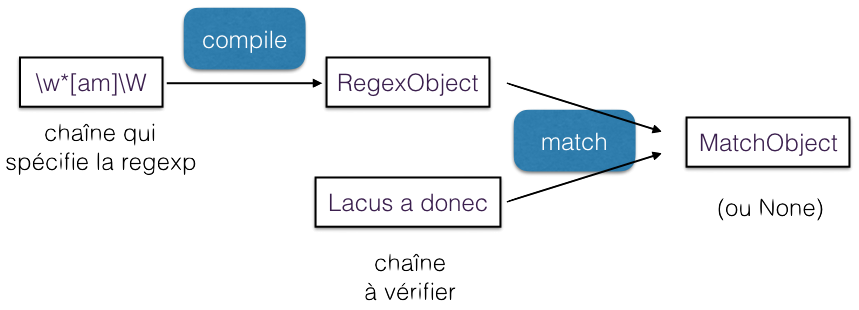
\includegraphics{medias/re-workflow.png}\\

    La méthode recommandée pour utiliser la librairie, lorsque vous avez le
même \emph{pattern} à appliquer à un grand nombre de chaînes, est de~:

\begin{itemize}
	\item 
	compiler \textbf{une seule fois} votre chaîne en un automate, qui est
	matérialisé par un objet de la classe \texttt{re.RegexObject}, en
	utilisant \texttt{re.compile},
	\item
	puis d'\textbf{utiliser directement cet
	objet} autant de fois que vous avez de chaînes.
\end{itemize}

    Nous avons utilisé dans les exemples plus haut (et nous continuerons
plus bas pour une meilleure lisibilité) des \textbf{fonctions de
commodité} du module, qui sont pratiques, par exemple, pour mettre au
point une expression régulière en mode interactif, mais qui ne
\textbf{sont pas forcément} adaptées dans tous les cas.\\

Ces fonctions de commodité fonctionnent toutes sur le même principe~:\\

\texttt{re.match(regexp,\ sample)} \(\Longleftrightarrow\)
\texttt{re.compile(regexp).match(sample)}\\

Donc à chaque fois qu'on utilise une fonction de commodité, on recompile
la chaîne en automate, ce qui, dès qu'on a plus d'une chaîne à traiter,
représente un surcoût.

    \begin{Verbatim}[commandchars=\\\{\}]
{\color{incolor}In [{\color{incolor}25}]:} \PY{c+c1}{\PYZsh{} au lieu de faire comme ci\PYZhy{}dessus:}
         
         \PY{c+c1}{\PYZsh{} imaginez 10**6 chaînes dans samples}
         \PY{k}{for} \PY{n}{sample} \PY{o+ow}{in} \PY{n}{samples}\PY{p}{:}
             \PY{n}{match} \PY{o}{=} \PY{n}{re}\PY{o}{.}\PY{n}{match}\PY{p}{(}\PY{n}{regexp3}\PY{p}{,} \PY{n}{sample}\PY{p}{)}
             \PY{n+nb}{print}\PY{p}{(}\PY{n}{f}\PY{l+s+s2}{\PYZdq{}}\PY{l+s+si}{\PYZob{}sample:\PYZgt{}16s\PYZcb{}}\PY{l+s+s2}{ → }\PY{l+s+s2}{\PYZob{}}\PY{l+s+s2}{nice(match)\PYZcb{}}\PY{l+s+s2}{\PYZdq{}}\PY{p}{)}    
\end{Verbatim}


    \begin{Verbatim}[commandchars=\\\{\}]
  890hj000nnm890 → Match!
 123abc456def789 → no
 8090abababab879 → no

    \end{Verbatim}

    \begin{Verbatim}[commandchars=\\\{\}]
{\color{incolor}In [{\color{incolor}26}]:} \PY{c+c1}{\PYZsh{} dans du vrai code on fera plutôt:}
         
         \PY{c+c1}{\PYZsh{} on compile la chaîne en automate une seule fois}
         \PY{n}{re\PYZus{}obj3} \PY{o}{=} \PY{n}{re}\PY{o}{.}\PY{n}{compile}\PY{p}{(}\PY{n}{regexp3}\PY{p}{)}
         
         \PY{c+c1}{\PYZsh{} ensuite on part directement de l\PYZsq{}automate}
         \PY{k}{for} \PY{n}{sample} \PY{o+ow}{in} \PY{n}{samples}\PY{p}{:}
             \PY{n}{match} \PY{o}{=} \PY{n}{re\PYZus{}obj3}\PY{o}{.}\PY{n}{match}\PY{p}{(}\PY{n}{sample}\PY{p}{)}
             \PY{n+nb}{print}\PY{p}{(}\PY{n}{f}\PY{l+s+s2}{\PYZdq{}}\PY{l+s+si}{\PYZob{}sample:\PYZgt{}16s\PYZcb{}}\PY{l+s+s2}{ → }\PY{l+s+s2}{\PYZob{}}\PY{l+s+s2}{nice(match)\PYZcb{}}\PY{l+s+s2}{\PYZdq{}}\PY{p}{)}
\end{Verbatim}


    \begin{Verbatim}[commandchars=\\\{\}]
  890hj000nnm890 → Match!
 123abc456def789 → no
 8090abababab879 → no

    \end{Verbatim}

    Cette deuxième version ne compile qu'une fois la chaîne en automate, et
donc est plus efficace.

    \hypertarget{les-muxe9thodes-sur-la-classe-regexobject}{%
\subparagraph{\texorpdfstring{Les méthodes sur la classe
\texttt{RegexObject}}{Les méthodes sur la classe RegexObject}}\label{les-muxe9thodes-sur-la-classe-regexobject}}

    Les objets de la classe \texttt{RegexObject} représentent donc
l'automate à état fini qui est le résultat de la compilation de
l'expression régulière. Pour résumer ce qu'on a déjà vu, les méthodes
les plus utiles sur un objet \texttt{RegexObject} sont~:

\begin{itemize}
	\item 
	\texttt{match} et \texttt{search}, qui cherchent un \emph{match} soit
	uniquement au début (\texttt{match}) ou n'importe où dans la chaîne
	(\texttt{search}),
	\item
	\texttt{findall} et \texttt{split} pour chercher
	toutes les occurences (\texttt{findall}) ou leur négatif
	(\texttt{split}),
	\item
	\texttt{sub} (qui aurait pu sans doute s'appeler
	\texttt{replace}, mais c'est comme ça) pour remplacer les occurrences de
	pattern.
\end{itemize}

    \hypertarget{exploiter-le-ruxe9sultat}{%
\subparagraph{Exploiter le résultat\\\\}\label{exploiter-le-ruxe9sultat}}

    Les \textbf{méthodes} disponibles sur la classe
\textbf{\texttt{re.MatchObject}} sont
\href{https://docs.python.org/3/library/re.html\#match-objects}{documentées
en détail ici}. On en a déjà rencontré quelques-unes, en voici à nouveau
un aperçu rapide.

    \begin{Verbatim}[commandchars=\\\{\}]
{\color{incolor}In [{\color{incolor}27}]:} \PY{c+c1}{\PYZsh{} exemple}
         \PY{n}{sample} \PY{o}{=} \PY{l+s+s2}{\PYZdq{}}\PY{l+s+s2}{    Isaac Newton, physicist}\PY{l+s+s2}{\PYZdq{}}
         \PY{n}{match} \PY{o}{=} \PY{n}{re}\PY{o}{.}\PY{n}{search}\PY{p}{(}\PY{l+s+sa}{r}\PY{l+s+s2}{\PYZdq{}}\PY{l+s+s2}{(}\PY{l+s+s2}{\PYZbs{}}\PY{l+s+s2}{w+) (?P\PYZlt{}name\PYZgt{}}\PY{l+s+s2}{\PYZbs{}}\PY{l+s+s2}{w+)}\PY{l+s+s2}{\PYZdq{}}\PY{p}{,} \PY{n}{sample}\PY{p}{)}
\end{Verbatim}


    \texttt{re} et \texttt{string} pour retrouver les données d'entrée du
match.

    \begin{Verbatim}[commandchars=\\\{\}]
{\color{incolor}In [{\color{incolor}28}]:} \PY{n}{match}\PY{o}{.}\PY{n}{string}
\end{Verbatim}


\begin{Verbatim}[commandchars=\\\{\}]
{\color{outcolor}Out[{\color{outcolor}28}]:} '    Isaac Newton, physicist'
\end{Verbatim}
            
    \begin{Verbatim}[commandchars=\\\{\}]
{\color{incolor}In [{\color{incolor}29}]:} \PY{n}{match}\PY{o}{.}\PY{n}{re}
\end{Verbatim}


\begin{Verbatim}[commandchars=\\\{\}]
{\color{outcolor}Out[{\color{outcolor}29}]:} re.compile(r'(\textbackslash{}w+) (?P<name>\textbackslash{}w+)', re.UNICODE)
\end{Verbatim}
            
    \texttt{group}, \texttt{groups}, \texttt{groupdict} pour retrouver les
morceaux de la chaîne d'entrée qui correspondent aux \textbf{groupes} de
la regexp. On peut y accéder par rang, ou par nom (comme on l'a vu plus
haut avec \texttt{needle}).

    \begin{Verbatim}[commandchars=\\\{\}]
{\color{incolor}In [{\color{incolor}30}]:} \PY{n}{match}\PY{o}{.}\PY{n}{groups}\PY{p}{(}\PY{p}{)}
\end{Verbatim}


\begin{Verbatim}[commandchars=\\\{\}]
{\color{outcolor}Out[{\color{outcolor}30}]:} ('Isaac', 'Newton')
\end{Verbatim}
            
    \begin{Verbatim}[commandchars=\\\{\}]
{\color{incolor}In [{\color{incolor}31}]:} \PY{n}{match}\PY{o}{.}\PY{n}{group}\PY{p}{(}\PY{l+m+mi}{1}\PY{p}{)}
\end{Verbatim}


\begin{Verbatim}[commandchars=\\\{\}]
{\color{outcolor}Out[{\color{outcolor}31}]:} 'Isaac'
\end{Verbatim}
            
    \begin{Verbatim}[commandchars=\\\{\}]
{\color{incolor}In [{\color{incolor}32}]:} \PY{n}{match}\PY{o}{.}\PY{n}{group}\PY{p}{(}\PY{l+s+s1}{\PYZsq{}}\PY{l+s+s1}{name}\PY{l+s+s1}{\PYZsq{}}\PY{p}{)}
\end{Verbatim}


\begin{Verbatim}[commandchars=\\\{\}]
{\color{outcolor}Out[{\color{outcolor}32}]:} 'Newton'
\end{Verbatim}
            
    \begin{Verbatim}[commandchars=\\\{\}]
{\color{incolor}In [{\color{incolor}33}]:} \PY{n}{match}\PY{o}{.}\PY{n}{group}\PY{p}{(}\PY{l+m+mi}{2}\PY{p}{)}
\end{Verbatim}


\begin{Verbatim}[commandchars=\\\{\}]
{\color{outcolor}Out[{\color{outcolor}33}]:} 'Newton'
\end{Verbatim}
            
    \begin{Verbatim}[commandchars=\\\{\}]
{\color{incolor}In [{\color{incolor}34}]:} \PY{n}{match}\PY{o}{.}\PY{n}{groupdict}\PY{p}{(}\PY{p}{)}
\end{Verbatim}


\begin{Verbatim}[commandchars=\\\{\}]
{\color{outcolor}Out[{\color{outcolor}34}]:} \{'name': 'Newton'\}
\end{Verbatim}
            
    Comme on le voit pour l'accès par rang \textbf{les indices commencent à
1} pour des raisons historiques (on peut déjà référencer
\texttt{\textbackslash{}1} en sed depuis la fin des années 70).\\

On peut aussi accéder au \textbf{groupe 0} comme étant la partie de la
chaîne de départ qui a effectivement été filtrée par l'expression
régulière, et qui peut tout à fait être au beau milieu de la chaîne de
départ, comme dans notre exemple

    \begin{Verbatim}[commandchars=\\\{\}]
{\color{incolor}In [{\color{incolor}35}]:} \PY{n}{match}\PY{o}{.}\PY{n}{group}\PY{p}{(}\PY{l+m+mi}{0}\PY{p}{)}
\end{Verbatim}


\begin{Verbatim}[commandchars=\\\{\}]
{\color{outcolor}Out[{\color{outcolor}35}]:} 'Isaac Newton'
\end{Verbatim}
            
    \texttt{expand} permet de faire une espèce de \texttt{str.format} avec
les valeurs des groupes.

    \begin{Verbatim}[commandchars=\\\{\}]
{\color{incolor}In [{\color{incolor}36}]:} \PY{n}{match}\PY{o}{.}\PY{n}{expand}\PY{p}{(}\PY{l+s+sa}{r}\PY{l+s+s2}{\PYZdq{}}\PY{l+s+s2}{last\PYZus{}name }\PY{l+s+s2}{\PYZbs{}}\PY{l+s+s2}{g\PYZlt{}name\PYZgt{} first\PYZus{}name }\PY{l+s+s2}{\PYZbs{}}\PY{l+s+s2}{1}\PY{l+s+s2}{\PYZdq{}}\PY{p}{)}
\end{Verbatim}


\begin{Verbatim}[commandchars=\\\{\}]
{\color{outcolor}Out[{\color{outcolor}36}]:} 'last\_name Newton first\_name Isaac'
\end{Verbatim}
            
    \texttt{span} pour connaître les index dans la chaîne d'entrée pour un
groupe donné.

    \begin{Verbatim}[commandchars=\\\{\}]
{\color{incolor}In [{\color{incolor}37}]:} \PY{n}{begin}\PY{p}{,} \PY{n}{end} \PY{o}{=} \PY{n}{match}\PY{o}{.}\PY{n}{span}\PY{p}{(}\PY{l+s+s1}{\PYZsq{}}\PY{l+s+s1}{name}\PY{l+s+s1}{\PYZsq{}}\PY{p}{)}
         \PY{n}{sample}\PY{p}{[}\PY{n}{begin}\PY{p}{:}\PY{n}{end}\PY{p}{]}
\end{Verbatim}


\begin{Verbatim}[commandchars=\\\{\}]
{\color{outcolor}Out[{\color{outcolor}37}]:} 'Newton'
\end{Verbatim}
            
    \hypertarget{les-diffuxe9rents-modes-flags}{%
\subparagraph{\texorpdfstring{Les différents modes
(\emph{flags})}{Les différents modes (flags)}}\label{les-diffuxe9rents-modes-flags}}

    Enfin il faut noter qu'on peut passer à \texttt{re.compile} un certain
nombre de \emph{flags} qui modifient globalement l'interprétation de la
chaîne, et qui peuvent rendre service.\\

    Vous trouverez
\href{https://docs.python.org/3/library/re.html\#module-contents}{une
liste exhaustive de ces \emph{flags} ici}. Ils ont en général un nom
long et parlant, et un alias court sur un seul caractère. Les plus
utiles sont sans doute~:

\begin{itemize}
	\item 
	\texttt{IGNORECASE} (\emph{alias} \texttt{I})
	pour, eh bien, ne pas faire la différence entre minuscules et
	majuscules,
	\item
	\texttt{UNICODE} (\emph{alias} \texttt{U}) pour rendre les
	séquences \texttt{\textbackslash{}w} et autres basées sur les propriétés
	des caractères dans la norme Unicode,
	\item
	\texttt{LOCALE} (\emph{alias}
	\texttt{L}) cette fois \texttt{\textbackslash{}w} dépend du
	\texttt{locale} courant,
	\item
	\texttt{MULTILINE} (\emph{alias} \texttt{M}), et
	\item
	\texttt{DOTALL} (\emph{alias} S) pour ces deux flags voir la
	discussion à la fin du complément.
\end{itemize}

    Comme c'est souvent le cas, on doit passer à \texttt{re.compile} un
\textbf{ou logique} (caractère \texttt{\textbar{}}) des différents flags
que l'on veut utiliser, c'est-à-dire qu'on fera par exemple

    \begin{Verbatim}[commandchars=\\\{\}]
{\color{incolor}In [{\color{incolor}38}]:} \PY{n}{regexp} \PY{o}{=} \PY{l+s+s2}{\PYZdq{}}\PY{l+s+s2}{a*b+}\PY{l+s+s2}{\PYZdq{}}
         \PY{n}{re\PYZus{}obj} \PY{o}{=} \PY{n}{re}\PY{o}{.}\PY{n}{compile}\PY{p}{(}\PY{n}{regexp}\PY{p}{,} \PY{n}{flags}\PY{o}{=}\PY{n}{re}\PY{o}{.}\PY{n}{IGNORECASE} \PY{o}{|} \PY{n}{re}\PY{o}{.}\PY{n}{DEBUG}\PY{p}{)}
\end{Verbatim}


    \begin{Verbatim}[commandchars=\\\{\}]
MAX\_REPEAT 0 MAXREPEAT
  LITERAL 97
MAX\_REPEAT 1 MAXREPEAT
  LITERAL 98

    \end{Verbatim}

    \begin{Verbatim}[commandchars=\\\{\}]
{\color{incolor}In [{\color{incolor}39}]:} \PY{c+c1}{\PYZsh{} on ignore la casse des caractères }
         \PY{n+nb}{print}\PY{p}{(}\PY{n}{regexp}\PY{p}{,} \PY{l+s+s2}{\PYZdq{}}\PY{l+s+s2}{\PYZhy{}\PYZgt{}}\PY{l+s+s2}{\PYZdq{}}\PY{p}{,} \PY{n}{nice}\PY{p}{(}\PY{n}{re\PYZus{}obj}\PY{o}{.}\PY{n}{match}\PY{p}{(}\PY{l+s+s2}{\PYZdq{}}\PY{l+s+s2}{AabB}\PY{l+s+s2}{\PYZdq{}}\PY{p}{)}\PY{p}{)}\PY{p}{)}
\end{Verbatim}


    \begin{Verbatim}[commandchars=\\\{\}]
a*b+ -> Match!

    \end{Verbatim}

    \hypertarget{comment-construire-une-expression-ruxe9guliuxe8re}{%
\subsubsection{Comment construire une expression
régulière}\label{comment-construire-une-expression-ruxe9guliuxe8re}}

    Nous pouvons à présent voir comment construire une expression régulière,
en essayant de rester synthétique (la
\href{https://docs.python.org/3/library/re.html}{documentation du module
\texttt{re}} en donne une version exhaustive).

    \hypertarget{la-brique-de-base-le-caractuxe8re}{%
\subparagraph{La brique de base : le
caractère\\\\}\label{la-brique-de-base-le-caractuxe8re}}

    Au commencement il faut spécifier des caractères.

\begin{itemize}
	\item 
    \textbf{un seul} caractère:
    \begin{itemize}
    	\item 
		vous le citez tel quel, en le précédent d'un backslash
		\texttt{\textbackslash{}} s'il a par ailleurs un sens spécial dans le
		micro-langage de regexps (comme \texttt{+}, \texttt{*}, \texttt{{[}},
		etc.);
	\end{itemize}
	\item	
	l'\textbf{attrape-tout} (\emph{wildcard}):
	\begin{itemize}
		\item 
		un point \texttt{.} signifie ``n'importe quel caractère'';
	\end{itemize}
	\item	
	\textbf{un ensemble}
	de caractères avec la notation \texttt{{[}...{]}} qui permet de décrire
	par exemple:
	\begin{itemize}
		\item 
		\texttt{{[}a1={]}} un ensemble in extenso, ici un
		caractère parmi \texttt{a}, \texttt{1}, ou \texttt{=},
		\item
		\texttt{{[}a-z{]}} un intervalle de caractères, ici de \texttt{a} à
		\texttt{z},
		\item
		\texttt{{[}15e-g{]}} un mélange des deux, ici un ensemble
		qui contiendrait \texttt{1}, \texttt{5}, \texttt{e}, \texttt{f} et
		\texttt{g},
		\item 	
		\texttt{{[}\^{}15e-g{]}} une \textbf{négation}, qui a
		\texttt{\^{}} comme premier caractère dans les \texttt{{[}{]}}, ici tout
		sauf l'ensemble précédent;
	\end{itemize}	
	\item
	un \textbf{ensemble prédéfini} de
	caractères, qui peuvent alors dépendre de l'environnement (UNICODE et
	LOCALE) avec entre autres les notations:
	\begin{itemize}
		\item 
		\texttt{\textbackslash{}w}
		les caractères alphanumériques, et \texttt{\textbackslash{}W} (les
		autres),
		\item
		\texttt{\textbackslash{}s} les caractères ``blancs'' -
		espace, tabulation, saut de ligne, etc., et \texttt{\textbackslash{}S}
		(les autres),
		\item
		\texttt{\textbackslash{}d} pour les chiffres, et
		\texttt{\textbackslash{}D} (les autres).
	\end{itemize}		
\end{itemize}

    \begin{Verbatim}[commandchars=\\\{\}]
{\color{incolor}In [{\color{incolor}40}]:} \PY{n}{sample} \PY{o}{=} \PY{l+s+s2}{\PYZdq{}}\PY{l+s+s2}{abcd}\PY{l+s+s2}{\PYZdq{}}
         
         \PY{k}{for} \PY{n}{regexp} \PY{o+ow}{in} \PY{p}{[}\PY{l+s+s1}{\PYZsq{}}\PY{l+s+s1}{abcd}\PY{l+s+s1}{\PYZsq{}}\PY{p}{,} \PY{l+s+s1}{\PYZsq{}}\PY{l+s+s1}{ab[cd][cd]}\PY{l+s+s1}{\PYZsq{}}\PY{p}{,} \PY{l+s+s1}{\PYZsq{}}\PY{l+s+s1}{ab[a\PYZhy{}z]d}\PY{l+s+s1}{\PYZsq{}}\PY{p}{,} \PY{l+s+sa}{r}\PY{l+s+s1}{\PYZsq{}}\PY{l+s+s1}{abc.}\PY{l+s+s1}{\PYZsq{}}\PY{p}{,} \PY{l+s+sa}{r}\PY{l+s+s1}{\PYZsq{}}\PY{l+s+s1}{abc}\PY{l+s+s1}{\PYZbs{}}\PY{l+s+s1}{.}\PY{l+s+s1}{\PYZsq{}}\PY{p}{]}\PY{p}{:}
             \PY{n}{match} \PY{o}{=} \PY{n}{re}\PY{o}{.}\PY{n}{match}\PY{p}{(}\PY{n}{regexp}\PY{p}{,} \PY{n}{sample}\PY{p}{)}
             \PY{n+nb}{print}\PY{p}{(}\PY{n}{f}\PY{l+s+s2}{\PYZdq{}}\PY{l+s+si}{\PYZob{}sample\PYZcb{}}\PY{l+s+s2}{ / }\PY{l+s+si}{\PYZob{}regexp:\PYZlt{}10s\PYZcb{}}\PY{l+s+s2}{ → }\PY{l+s+s2}{\PYZob{}}\PY{l+s+s2}{nice(match)\PYZcb{}}\PY{l+s+s2}{\PYZdq{}}\PY{p}{)}
\end{Verbatim}


    \begin{Verbatim}[commandchars=\\\{\}]
abcd / abcd       → Match!
abcd / ab[cd][cd] → Match!
abcd / ab[a-z]d   → Match!
abcd / abc.       → Match!
abcd / abc\textbackslash{}.      → no

    \end{Verbatim}

    Pour ce dernier exemple, comme on a backslashé le \texttt{.} il faut que
la chaîne en entrée contienne vraiment un \texttt{.}

    \begin{Verbatim}[commandchars=\\\{\}]
{\color{incolor}In [{\color{incolor}41}]:} \PY{n+nb}{print}\PY{p}{(}\PY{n}{nice}\PY{p}{(}\PY{n}{re}\PY{o}{.}\PY{n}{match} \PY{p}{(}\PY{l+s+sa}{r}\PY{l+s+s2}{\PYZdq{}}\PY{l+s+s2}{abc}\PY{l+s+s2}{\PYZbs{}}\PY{l+s+s2}{.}\PY{l+s+s2}{\PYZdq{}}\PY{p}{,} \PY{l+s+s2}{\PYZdq{}}\PY{l+s+s2}{abc.}\PY{l+s+s2}{\PYZdq{}}\PY{p}{)}\PY{p}{)}\PY{p}{)}
\end{Verbatim}


    \begin{Verbatim}[commandchars=\\\{\}]
Match!

    \end{Verbatim}

    \hypertarget{en-suxe9rie-ou-en-paralluxe8le}{%
\subparagraph{En série ou en
parallèle}\label{en-suxe9rie-ou-en-paralluxe8le}}

    Si je fais une analogie avec les montages électriques, jusqu'ici on a vu
le montage en série, on met des expressions régulières bout à bout qui
filtrent (\texttt{match}) la chaine en entrée séquentiellement du début
à la fin. On a \emph{un peu} de marge pour spécifier des alternatives,
lorsqu'on fait par exemple

\begin{verbatim}
"ab[cd]ef"
\end{verbatim}

mais c'est limité à \textbf{un seul} caractère. Si on veut reconnaitre
deux mots qui n'ont pas grand-chose à voir comme \texttt{abc}
\textbf{ou} \texttt{def}, il faut en quelque sorte mettre deux regexps
en parallèle, et c'est ce que permet l'opérateur \texttt{\textbar{}}

    \begin{Verbatim}[commandchars=\\\{\}]
{\color{incolor}In [{\color{incolor}42}]:} \PY{n}{regexp} \PY{o}{=} \PY{l+s+s2}{\PYZdq{}}\PY{l+s+s2}{abc|def}\PY{l+s+s2}{\PYZdq{}}
         
         \PY{k}{for} \PY{n}{sample} \PY{o+ow}{in} \PY{p}{[}\PY{l+s+s1}{\PYZsq{}}\PY{l+s+s1}{abc}\PY{l+s+s1}{\PYZsq{}}\PY{p}{,} \PY{l+s+s1}{\PYZsq{}}\PY{l+s+s1}{def}\PY{l+s+s1}{\PYZsq{}}\PY{p}{,} \PY{l+s+s1}{\PYZsq{}}\PY{l+s+s1}{aef}\PY{l+s+s1}{\PYZsq{}}\PY{p}{]}\PY{p}{:}
             \PY{n}{match} \PY{o}{=} \PY{n}{re}\PY{o}{.}\PY{n}{match}\PY{p}{(}\PY{n}{regexp}\PY{p}{,} \PY{n}{sample}\PY{p}{)}
             \PY{n+nb}{print}\PY{p}{(}\PY{n}{f}\PY{l+s+s2}{\PYZdq{}}\PY{l+s+si}{\PYZob{}sample\PYZcb{}}\PY{l+s+s2}{ / }\PY{l+s+si}{\PYZob{}regexp\PYZcb{}}\PY{l+s+s2}{ → }\PY{l+s+s2}{\PYZob{}}\PY{l+s+s2}{nice(match)\PYZcb{}}\PY{l+s+s2}{\PYZdq{}}\PY{p}{)}
\end{Verbatim}


    \begin{Verbatim}[commandchars=\\\{\}]
abc / abc|def → Match!
def / abc|def → Match!
aef / abc|def → no

    \end{Verbatim}

    \hypertarget{fins-de-chauxeene}{%
\subparagraph{Fin(s) de chaîne\\\\}\label{fins-de-chauxeene}}

    Selon que vous utilisez \texttt{match} ou \texttt{search}, vous précisez
si vous vous intéressez uniquement à un match en début (\texttt{match})
ou n'importe où (\texttt{search}) dans la chaîne.\\

Mais indépendamment de cela, il peut être intéressant de ``coller''
l'expression en début ou en fin de ligne, et pour ça il existe des
caractères spéciaux:

\begin{itemize}
	\item
	\texttt{\^{}} lorsqu'il est utilisé comme un
	caractère (c'est à dire pas en début de \texttt{{[}{]}}) signifie un
	début de chaîne;
	\item
	\texttt{\textbackslash{}A} a le même sens (sauf en
	mode MULTILINE), et je le recommande de préférence à \texttt{\^{}} qui
	est déjà pas mal surchargé;
	\item
	\texttt{\$} matche une fin de ligne;
	\item
	\texttt{\textbackslash{}Z} est voisin mais pas tout à fait identique.
\end{itemize}

Reportez-vous à la documentation pour le détails des différences.
Attention aussi à entrer le \texttt{\^{}} correctement, il vous faut le
caractère ASCII et non un voisin dans la ménagerie Unicode.

    \begin{Verbatim}[commandchars=\\\{\}]
{\color{incolor}In [{\color{incolor}43}]:} \PY{n}{sample} \PY{o}{=} \PY{l+s+s1}{\PYZsq{}}\PY{l+s+s1}{abcd}\PY{l+s+s1}{\PYZsq{}}
         
         \PY{k}{for} \PY{n}{regexp} \PY{o+ow}{in} \PY{p}{[} \PY{l+s+sa}{r}\PY{l+s+s1}{\PYZsq{}}\PY{l+s+s1}{bc}\PY{l+s+s1}{\PYZsq{}}\PY{p}{,} \PY{l+s+sa}{r}\PY{l+s+s1}{\PYZsq{}}\PY{l+s+s1}{\PYZbs{}}\PY{l+s+s1}{Aabc}\PY{l+s+s1}{\PYZsq{}}\PY{p}{,} \PY{l+s+sa}{r}\PY{l+s+s1}{\PYZsq{}}\PY{l+s+s1}{\PYZca{}abc}\PY{l+s+s1}{\PYZsq{}}\PY{p}{,} 
                         \PY{l+s+sa}{r}\PY{l+s+s1}{\PYZsq{}}\PY{l+s+s1}{\PYZbs{}}\PY{l+s+s1}{Abc}\PY{l+s+s1}{\PYZsq{}}\PY{p}{,} \PY{l+s+sa}{r}\PY{l+s+s1}{\PYZsq{}}\PY{l+s+s1}{\PYZca{}bc}\PY{l+s+s1}{\PYZsq{}}\PY{p}{,} \PY{l+s+sa}{r}\PY{l+s+s1}{\PYZsq{}}\PY{l+s+s1}{bcd}\PY{l+s+s1}{\PYZbs{}}\PY{l+s+s1}{Z}\PY{l+s+s1}{\PYZsq{}}\PY{p}{,} 
                         \PY{l+s+sa}{r}\PY{l+s+s1}{\PYZsq{}}\PY{l+s+s1}{bcd\PYZdl{}}\PY{l+s+s1}{\PYZsq{}}\PY{p}{,} \PY{l+s+sa}{r}\PY{l+s+s1}{\PYZsq{}}\PY{l+s+s1}{bc}\PY{l+s+s1}{\PYZbs{}}\PY{l+s+s1}{Z}\PY{l+s+s1}{\PYZsq{}}\PY{p}{,} \PY{l+s+sa}{r}\PY{l+s+s1}{\PYZsq{}}\PY{l+s+s1}{bc\PYZdl{}}\PY{l+s+s1}{\PYZsq{}} \PY{p}{]}\PY{p}{:}
             \PY{n}{match} \PY{o}{=} \PY{n}{re}\PY{o}{.}\PY{n}{match}\PY{p}{(}\PY{n}{regexp}\PY{p}{,} \PY{n}{sample}\PY{p}{)}
             \PY{n}{search} \PY{o}{=} \PY{n}{re}\PY{o}{.}\PY{n}{search}\PY{p}{(}\PY{n}{regexp}\PY{p}{,} \PY{n}{sample}\PY{p}{)}
             \PY{n+nb}{print}\PY{p}{(}\PY{n}{f}\PY{l+s+s2}{\PYZdq{}}\PY{l+s+si}{\PYZob{}sample\PYZcb{}}\PY{l+s+s2}{ / }\PY{l+s+si}{\PYZob{}regexp:5s\PYZcb{}}\PY{l+s+s2}{ match → }\PY{l+s+s2}{\PYZob{}}\PY{l+s+s2}{nice(match):6s\PYZcb{} search → }\PY{l+s+s2}{\PYZob{}}\PY{l+s+s2}{nice(search)\PYZcb{}}\PY{l+s+s2}{\PYZdq{}}\PY{p}{)}
\end{Verbatim}


    \begin{Verbatim}[commandchars=\\\{\}]
abcd / bc    match → no     search → Match!
abcd / \textbackslash{}Aabc match → Match! search → Match!
abcd / \^{}abc  match → Match! search → Match!
abcd / \textbackslash{}Abc  match → no     search → no
abcd / \^{}bc   match → no     search → no
abcd / bcd\textbackslash{}Z match → no     search → Match!
abcd / bcd\$  match → no     search → Match!
abcd / bc\textbackslash{}Z  match → no     search → no
abcd / bc\$   match → no     search → no

    \end{Verbatim}

    On a en effet bien le pattern \texttt{bc} dans la chaine en entrée, mais
il n'est ni au début ni à la fin.

    \hypertarget{parenthuxe9ser---grouper}{%
\subparagraph{Parenthéser - (grouper)\\\\}\label{parenthuxe9ser---grouper}}

    Pour pouvoir faire des montages élaborés, il faut pouvoir parenthéser.

    \begin{Verbatim}[commandchars=\\\{\}]
{\color{incolor}In [{\color{incolor}44}]:} \PY{c+c1}{\PYZsh{} une parenthése dans une RE }
         \PY{c+c1}{\PYZsh{} pour mettre en ligne:}
         \PY{c+c1}{\PYZsh{} un début \PYZsq{}a\PYZsq{}, }
         \PY{c+c1}{\PYZsh{} un milieu \PYZsq{}bc\PYZsq{} ou \PYZsq{}de\PYZsq{} }
         \PY{c+c1}{\PYZsh{} et une fin \PYZsq{}f\PYZsq{}}
         \PY{n}{regexp} \PY{o}{=} \PY{l+s+s2}{\PYZdq{}}\PY{l+s+s2}{a(bc|de)f}\PY{l+s+s2}{\PYZdq{}}
\end{Verbatim}

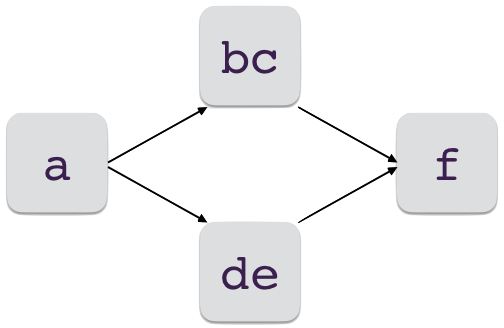
\includegraphics{medias/re-serie-parallele.png}\\
    

    \begin{Verbatim}[commandchars=\\\{\}]
{\color{incolor}In [{\color{incolor}45}]:} \PY{k}{for} \PY{n}{sample} \PY{o+ow}{in} \PY{p}{[}\PY{l+s+s1}{\PYZsq{}}\PY{l+s+s1}{abcf}\PY{l+s+s1}{\PYZsq{}}\PY{p}{,} \PY{l+s+s1}{\PYZsq{}}\PY{l+s+s1}{adef}\PY{l+s+s1}{\PYZsq{}}\PY{p}{,}  \PY{l+s+s1}{\PYZsq{}}\PY{l+s+s1}{abef}\PY{l+s+s1}{\PYZsq{}}\PY{p}{,} \PY{l+s+s1}{\PYZsq{}}\PY{l+s+s1}{abf}\PY{l+s+s1}{\PYZsq{}}\PY{p}{]}\PY{p}{:}
             \PY{n}{match} \PY{o}{=} \PY{n}{re}\PY{o}{.}\PY{n}{match}\PY{p}{(}\PY{n}{regexp}\PY{p}{,} \PY{n}{sample}\PY{p}{)}
             \PY{n+nb}{print}\PY{p}{(}\PY{n}{f}\PY{l+s+s2}{\PYZdq{}}\PY{l+s+si}{\PYZob{}sample:\PYZgt{}4s\PYZcb{}}\PY{l+s+s2}{ → }\PY{l+s+s2}{\PYZob{}}\PY{l+s+s2}{nice(match)\PYZcb{}}\PY{l+s+s2}{\PYZdq{}}\PY{p}{)}
\end{Verbatim}


    \begin{Verbatim}[commandchars=\\\{\}]
abcf → Match!
adef → Match!
abef → no
 abf → no

    \end{Verbatim}

    Les parenthèses jouent un rôle additionel de \textbf{groupe}, ce qui
signifie qu'on \textbf{peut retrouver} le texte correspondant à
l'expression régulière comprise dans les \texttt{()}. Par exemple, pour
le premier match

    \begin{Verbatim}[commandchars=\\\{\}]
{\color{incolor}In [{\color{incolor}46}]:} \PY{n}{sample} \PY{o}{=} \PY{l+s+s1}{\PYZsq{}}\PY{l+s+s1}{abcf}\PY{l+s+s1}{\PYZsq{}}
         \PY{n}{match} \PY{o}{=} \PY{n}{re}\PY{o}{.}\PY{n}{match}\PY{p}{(}\PY{n}{regexp}\PY{p}{,} \PY{n}{sample}\PY{p}{)}
         \PY{n+nb}{print}\PY{p}{(}\PY{n}{f}\PY{l+s+s2}{\PYZdq{}}\PY{l+s+si}{\PYZob{}sample\PYZcb{}}\PY{l+s+s2}{, }\PY{l+s+si}{\PYZob{}regexp\PYZcb{}}\PY{l+s+s2}{ → }\PY{l+s+s2}{\PYZob{}}\PY{l+s+s2}{match.groups()\PYZcb{}}\PY{l+s+s2}{\PYZdq{}}\PY{p}{)}
\end{Verbatim}


    \begin{Verbatim}[commandchars=\\\{\}]
abcf, a(bc|de)f → ('bc',)

    \end{Verbatim}

    dans cet exemple, on n'a utilisé qu'un seul groupe \texttt{()}, et le
morceau de chaîne qui correspond à ce groupe se trouve donc être le seul
groupe retourné par \texttt{MatchObject.group}.

    \hypertarget{compter-les-ruxe9puxe9titions}{%
\subparagraph{Compter les
répétitions\\\\}\label{compter-les-ruxe9puxe9titions}}

    Vous disposez des opérateurs suivants~:
    
\begin{itemize}
	\item 
   	\texttt{*} l'étoile qui
	signifie n'importe quel nombre, même nul, d'occurrences - par exemple,
	\texttt{(ab)*} pour indiquer
	\texttt{\textquotesingle{}\textquotesingle{}} ou
	\texttt{\textquotesingle{}ab\textquotesingle{}} ou
	\texttt{\textquotesingle{}abab\textquotesingle{}} ou etc.,
	\item
	\texttt{+}
	le plus qui signifie au moins une occurrence - e.g. \texttt{(ab)+} pour
	\texttt{ab} ou \texttt{abab} ou \texttt{ababab} ou etc,
	\item
	\texttt{?} qui
	indique une option, c'est-à-dire 0 ou 1 occurence - autrement dit
	\texttt{(ab)?} matche \texttt{\textquotesingle{}\textquotesingle{}} ou
	\texttt{ab},
	\item
	\texttt{\{n\}} pour exactement n occurrences de
	\texttt{(ab)} - e.g. \texttt{(ab)\{3\}} qui serait exactement équivalent
	à \texttt{ababab},
	\item
	\texttt{\{m,n\}} entre m et n fois inclusivement.
\end{itemize}

    \begin{Verbatim}[commandchars=\\\{\}]
{\color{incolor}In [{\color{incolor}47}]:} \PY{n}{samples} \PY{o}{=} \PY{p}{[}\PY{n}{n}\PY{o}{*}\PY{l+s+s1}{\PYZsq{}}\PY{l+s+s1}{ab}\PY{l+s+s1}{\PYZsq{}} \PY{k}{for} \PY{n}{n} \PY{o+ow}{in} \PY{p}{[}\PY{l+m+mi}{0}\PY{p}{,} \PY{l+m+mi}{1}\PY{p}{,} \PY{l+m+mi}{3}\PY{p}{,} \PY{l+m+mi}{4}\PY{p}{]}\PY{p}{]} \PY{o}{+} \PY{p}{[}\PY{l+s+s1}{\PYZsq{}}\PY{l+s+s1}{baba}\PY{l+s+s1}{\PYZsq{}}\PY{p}{]}
         
         \PY{k}{for} \PY{n}{regexp} \PY{o+ow}{in} \PY{p}{[}\PY{l+s+s1}{\PYZsq{}}\PY{l+s+s1}{(ab)*}\PY{l+s+s1}{\PYZsq{}}\PY{p}{,} \PY{l+s+s1}{\PYZsq{}}\PY{l+s+s1}{(ab)+}\PY{l+s+s1}{\PYZsq{}}\PY{p}{,} \PY{l+s+s1}{\PYZsq{}}\PY{l+s+s1}{(ab)}\PY{l+s+si}{\PYZob{}3\PYZcb{}}\PY{l+s+s1}{\PYZsq{}}\PY{p}{,} \PY{l+s+s1}{\PYZsq{}}\PY{l+s+s1}{(ab)}\PY{l+s+s1}{\PYZob{}}\PY{l+s+s1}{3,4\PYZcb{}}\PY{l+s+s1}{\PYZsq{}}\PY{p}{]}\PY{p}{:}
             \PY{c+c1}{\PYZsh{} on ajoute \PYZbs{}A \PYZbs{}Z pour matcher toute la chaine}
             \PY{n}{line\PYZus{}regexp} \PY{o}{=} \PY{l+s+sa}{r}\PY{l+s+s2}{\PYZdq{}}\PY{l+s+s2}{\PYZbs{}}\PY{l+s+s2}{A}\PY{l+s+si}{\PYZob{}\PYZcb{}}\PY{l+s+s2}{\PYZbs{}}\PY{l+s+s2}{Z}\PY{l+s+s2}{\PYZdq{}}\PY{o}{.}\PY{n}{format}\PY{p}{(}\PY{n}{regexp}\PY{p}{)}
             \PY{k}{for} \PY{n}{sample} \PY{o+ow}{in} \PY{n}{samples}\PY{p}{:}
                 \PY{n}{match} \PY{o}{=} \PY{n}{re}\PY{o}{.}\PY{n}{match}\PY{p}{(}\PY{n}{line\PYZus{}regexp}\PY{p}{,} \PY{n}{sample}\PY{p}{)}
                 \PY{n+nb}{print}\PY{p}{(}\PY{n}{f}\PY{l+s+s2}{\PYZdq{}}\PY{l+s+si}{\PYZob{}sample:\PYZgt{}8s\PYZcb{}}\PY{l+s+s2}{ / }\PY{l+s+si}{\PYZob{}line\PYZus{}regexp:14s\PYZcb{}}\PY{l+s+s2}{ → }\PY{l+s+s2}{\PYZob{}}\PY{l+s+s2}{nice(match)\PYZcb{}}\PY{l+s+s2}{\PYZdq{}}\PY{p}{)}
\end{Verbatim}


    \begin{Verbatim}[commandchars=\\\{\}]
         / \textbackslash{}A(ab)*\textbackslash{}Z      → Match!
      ab / \textbackslash{}A(ab)*\textbackslash{}Z      → Match!
  ababab / \textbackslash{}A(ab)*\textbackslash{}Z      → Match!
abababab / \textbackslash{}A(ab)*\textbackslash{}Z      → Match!
    baba / \textbackslash{}A(ab)*\textbackslash{}Z      → no
         / \textbackslash{}A(ab)+\textbackslash{}Z      → no
      ab / \textbackslash{}A(ab)+\textbackslash{}Z      → Match!
  ababab / \textbackslash{}A(ab)+\textbackslash{}Z      → Match!
abababab / \textbackslash{}A(ab)+\textbackslash{}Z      → Match!
    baba / \textbackslash{}A(ab)+\textbackslash{}Z      → no
         / \textbackslash{}A(ab)\{3\}\textbackslash{}Z    → no
      ab / \textbackslash{}A(ab)\{3\}\textbackslash{}Z    → no
  ababab / \textbackslash{}A(ab)\{3\}\textbackslash{}Z    → Match!
abababab / \textbackslash{}A(ab)\{3\}\textbackslash{}Z    → no
    baba / \textbackslash{}A(ab)\{3\}\textbackslash{}Z    → no
         / \textbackslash{}A(ab)\{3,4\}\textbackslash{}Z  → no
      ab / \textbackslash{}A(ab)\{3,4\}\textbackslash{}Z  → no
  ababab / \textbackslash{}A(ab)\{3,4\}\textbackslash{}Z  → Match!
abababab / \textbackslash{}A(ab)\{3,4\}\textbackslash{}Z  → Match!
    baba / \textbackslash{}A(ab)\{3,4\}\textbackslash{}Z  → no

    \end{Verbatim}

    \hypertarget{groupes-et-contraintes}{%
\subparagraph{Groupes et contraintes\\\\}\label{groupes-et-contraintes}}

    Nous avons déjà vu un exemple de groupe nommé (voir \texttt{needle} plus
haut), les opérateurs que l'on peut citer dans cette catégorie sont~:

\begin{itemize}
	\item 
	\texttt{(...)} les parenthèses définissent un groupe anonyme,
	\item
	\texttt{(?P\textless{}name\textgreater{}...)} définit un groupe nommé,
	\item
	\texttt{(?:...)} permet de mettre des parenthèses mais sans créer un
	groupe, pour optimiser l'exécution puisqu'on n'a pas besoin de conserver
	les liens vers la chaîne d'entrée,
	\item
	\texttt{(?P=name)} qui ne matche
	que si l'on retrouve à cet endroit de l'entrée la même sous-chaîne que
	celle trouvée pour le groupe \texttt{name} en amont,
	\item
	enfin
	\texttt{(?=...)}, \texttt{(?!...)}et \texttt{(?\textless{}=...)}
	permettent des contraintes encore plus élaborées, nous vous laissons le
	soin d'expérimenter avec elles si vous êtes intéressés; sachez toutefois
	que l'utilisation de telles constructions peut en théorie rendre
	l'interprétation de votre expression régulière beaucoup moins efficace.
\end{itemize}

    \hypertarget{greedy-vs-non-greedy}{%
\subparagraph{\texorpdfstring{Greedy \emph{vs}
non-greedy}{Greedy vs non-greedy}\\\\}\label{greedy-vs-non-greedy}}

    Lorsqu'on stipule une répétition un nombre indéfini de fois, il se peut
qu'il existe \textbf{plusieurs} façons de filtrer l'entrée avec
l'expression régulière. Que ce soit avec \texttt{*}, ou \texttt{+}, ou
\texttt{?}, l'algorithme va toujours essayer de trouver la
\textbf{séquence la plus longue}, c'est pourquoi on qualifie l'approche
de \emph{greedy} - quelque chose comme glouton en français.

    \begin{Verbatim}[commandchars=\\\{\}]
{\color{incolor}In [{\color{incolor}48}]:} \PY{c+c1}{\PYZsh{} un fragment d\PYZsq{}HTML }
         \PY{n}{line}\PY{o}{=}\PY{l+s+s1}{\PYZsq{}}\PY{l+s+s1}{\PYZlt{}h1\PYZgt{}Title\PYZlt{}/h1\PYZgt{}}\PY{l+s+s1}{\PYZsq{}}
         
         \PY{c+c1}{\PYZsh{} si on cherche un texte quelconque entre crochets}
         \PY{c+c1}{\PYZsh{} c\PYZsq{}est\PYZhy{}à\PYZhy{}dire l\PYZsq{}expression régulière \PYZdq{}\PYZlt{}.*\PYZgt{}\PYZdq{}}
         \PY{n}{re\PYZus{}greedy} \PY{o}{=} \PY{l+s+s1}{\PYZsq{}}\PY{l+s+s1}{\PYZlt{}.*\PYZgt{}}\PY{l+s+s1}{\PYZsq{}}
         
         \PY{c+c1}{\PYZsh{} on obtient ceci}
         \PY{c+c1}{\PYZsh{} on rappelle que group(0) montre la partie du fragment}
         \PY{c+c1}{\PYZsh{} HTML qui matche l\PYZsq{}expression régulière}
         \PY{n}{match} \PY{o}{=} \PY{n}{re}\PY{o}{.}\PY{n}{match}\PY{p}{(}\PY{n}{re\PYZus{}greedy}\PY{p}{,} \PY{n}{line}\PY{p}{)}
         \PY{n}{match}\PY{o}{.}\PY{n}{group}\PY{p}{(}\PY{l+m+mi}{0}\PY{p}{)}
\end{Verbatim}


\begin{Verbatim}[commandchars=\\\{\}]
{\color{outcolor}Out[{\color{outcolor}48}]:} '<h1>Title</h1>'
\end{Verbatim}
            
    Ça n'est pas forcément ce qu'on voulait faire, aussi on peut spécifier
l'approche inverse, c'est-à-dire de trouver la \textbf{plus-petite}
chaîne qui matche, dans une approche dite \emph{non-greedy}, avec les
opérateurs suivants~:

\begin{itemize}
	\item 
	\texttt{*?} : \texttt{*} mais \emph{non-greedy},
	\item
	\texttt{+?} : \texttt{+} mais \emph{non-greedy},
	\item 
	\texttt{??} : \texttt{?} mais \emph{non-greedy},
\end{itemize}

    \begin{Verbatim}[commandchars=\\\{\}]
{\color{incolor}In [{\color{incolor}49}]:} \PY{c+c1}{\PYZsh{} ici on va remplacer * par *? pour rendre l\PYZsq{}opérateur * non\PYZhy{}greedy}
         \PY{n}{re\PYZus{}non\PYZus{}greedy} \PY{o}{=} \PY{n}{re\PYZus{}greedy} \PY{o}{=} \PY{l+s+s1}{\PYZsq{}}\PY{l+s+s1}{\PYZlt{}.*?\PYZgt{}}\PY{l+s+s1}{\PYZsq{}}
         
         \PY{c+c1}{\PYZsh{} mais on continue à cherche un texte entre \PYZlt{}\PYZgt{} naturellement}
         \PY{c+c1}{\PYZsh{} si bien que cette fois, on obtient}
         \PY{n}{match} \PY{o}{=} \PY{n}{re}\PY{o}{.}\PY{n}{match}\PY{p}{(}\PY{n}{re\PYZus{}non\PYZus{}greedy}\PY{p}{,} \PY{n}{line}\PY{p}{)}
         \PY{n}{match}\PY{o}{.}\PY{n}{group}\PY{p}{(}\PY{l+m+mi}{0}\PY{p}{)}
\end{Verbatim}


\begin{Verbatim}[commandchars=\\\{\}]
{\color{outcolor}Out[{\color{outcolor}49}]:} '<h1>'
\end{Verbatim}
            
    \hypertarget{sagissant-du-traitement-des-fins-de-ligne}{%
\subparagraph{S'agissant du traitement des fins de
ligne\\\\}\label{sagissant-du-traitement-des-fins-de-ligne}}

    Il peut être utile, pour conclure cette présentation, de préciser un peu
le comportement de la librairie vis-à-vis des fins de ligne.\\

Historiquement, les expressions régulières telles qu'on les trouve dans
les librairies C, donc dans \texttt{sed}, \texttt{grep} et autre
utilitaires Unix, sont associées au modèle mental où on filtre les
entrées ligne par ligne.\\

Le module \texttt{re} en garde des traces, puisque

    \begin{Verbatim}[commandchars=\\\{\}]
{\color{incolor}In [{\color{incolor}50}]:} \PY{c+c1}{\PYZsh{} un exemple de traitement des \PYZsq{}newline\PYZsq{} }
         \PY{n}{sample} \PY{o}{=} \PY{l+s+s2}{\PYZdq{}\PYZdq{}\PYZdq{}}\PY{l+s+s2}{une entrée}
         \PY{l+s+s2}{sur}
         \PY{l+s+s2}{plusieurs}
         \PY{l+s+s2}{lignes}
         \PY{l+s+s2}{\PYZdq{}\PYZdq{}\PYZdq{}}
\end{Verbatim}


    \begin{Verbatim}[commandchars=\\\{\}]
{\color{incolor}In [{\color{incolor}51}]:} \PY{n}{match} \PY{o}{=} \PY{n}{re}\PY{o}{.}\PY{n}{compile}\PY{p}{(}\PY{l+s+s2}{\PYZdq{}}\PY{l+s+s2}{(.*)}\PY{l+s+s2}{\PYZdq{}}\PY{p}{)}\PY{o}{.}\PY{n}{match}\PY{p}{(}\PY{n}{sample}\PY{p}{)}
         \PY{n}{match}\PY{o}{.}\PY{n}{groups}\PY{p}{(}\PY{p}{)}
\end{Verbatim}


\begin{Verbatim}[commandchars=\\\{\}]
{\color{outcolor}Out[{\color{outcolor}51}]:} ('une entrée',)
\end{Verbatim}
            
    Vous voyez donc que l'attrape-tout
\texttt{\textquotesingle{}.\textquotesingle{}} en fait n'attrape pas le
caractère de fin de ligne \texttt{\textbackslash{}n}, puisque si c'était
le cas et compte tenu du coté \emph{greedy} de l'algorithme on devrait
voir ici tout le contenu de \texttt{sample}. Il existe un \emph{flag}
\texttt{re.DOTALL} qui permet de faire de \texttt{.} un vrai
attrape-tout qui capture aussi les \emph{newline}

    \begin{Verbatim}[commandchars=\\\{\}]
{\color{incolor}In [{\color{incolor}52}]:} \PY{n}{match} \PY{o}{=} \PY{n}{re}\PY{o}{.}\PY{n}{compile}\PY{p}{(}\PY{l+s+s2}{\PYZdq{}}\PY{l+s+s2}{(.*)}\PY{l+s+s2}{\PYZdq{}}\PY{p}{,} \PY{n}{flags}\PY{o}{=}\PY{n}{re}\PY{o}{.}\PY{n}{DOTALL}\PY{p}{)}\PY{o}{.}\PY{n}{match}\PY{p}{(}\PY{n}{sample}\PY{p}{)}
         \PY{n}{match}\PY{o}{.}\PY{n}{groups}\PY{p}{(}\PY{p}{)}
\end{Verbatim}


\begin{Verbatim}[commandchars=\\\{\}]
{\color{outcolor}Out[{\color{outcolor}52}]:} ('une entrée\textbackslash{}nsur\textbackslash{}nplusieurs\textbackslash{}nlignes\textbackslash{}n',)
\end{Verbatim}
            
    Cela dit, le caractère \emph{newline} est par ailleurs considéré comme
un caractère comme un autre, on peut le mentionner \textbf{dans une
regexp} comme les autres. Voici quelques exemples pour illustrer tout
ceci

    \begin{Verbatim}[commandchars=\\\{\}]
{\color{incolor}In [{\color{incolor}53}]:} \PY{c+c1}{\PYZsh{} sans mettre le flag unicode \PYZbs{}w ne matche que l\PYZsq{}ASCII}
         \PY{n}{match} \PY{o}{=} \PY{n}{re}\PY{o}{.}\PY{n}{compile}\PY{p}{(}\PY{l+s+s2}{\PYZdq{}}\PY{l+s+s2}{([}\PY{l+s+s2}{\PYZbs{}}\PY{l+s+s2}{w ]*)}\PY{l+s+s2}{\PYZdq{}}\PY{p}{)}\PY{o}{.}\PY{n}{match}\PY{p}{(}\PY{n}{sample}\PY{p}{)}
         \PY{n}{match}\PY{o}{.}\PY{n}{groups}\PY{p}{(}\PY{p}{)}
\end{Verbatim}


\begin{Verbatim}[commandchars=\\\{\}]
{\color{outcolor}Out[{\color{outcolor}53}]:} ('une entrée',)
\end{Verbatim}
            
    \begin{Verbatim}[commandchars=\\\{\}]
{\color{incolor}In [{\color{incolor}54}]:} \PY{c+c1}{\PYZsh{} sans mettre le flag unicode \PYZbs{}w ne matche que l\PYZsq{}ASCII}
         \PY{n}{match} \PY{o}{=} \PY{n}{re}\PY{o}{.}\PY{n}{compile}\PY{p}{(}\PY{l+s+s2}{\PYZdq{}}\PY{l+s+s2}{([}\PY{l+s+s2}{\PYZbs{}}\PY{l+s+s2}{w ]*)}\PY{l+s+s2}{\PYZdq{}}\PY{p}{,} \PY{n}{flags}\PY{o}{=}\PY{n}{re}\PY{o}{.}\PY{n}{U}\PY{p}{)}\PY{o}{.}\PY{n}{match}\PY{p}{(}\PY{n}{sample}\PY{p}{)}
         \PY{n}{match}\PY{o}{.}\PY{n}{groups}\PY{p}{(}\PY{p}{)}
\end{Verbatim}


\begin{Verbatim}[commandchars=\\\{\}]
{\color{outcolor}Out[{\color{outcolor}54}]:} ('une entrée',)
\end{Verbatim}
            
    \begin{Verbatim}[commandchars=\\\{\}]
{\color{incolor}In [{\color{incolor}55}]:} \PY{c+c1}{\PYZsh{} si on ajoute \PYZbs{}n à la liste des caractères attendus }
         \PY{c+c1}{\PYZsh{} on obtient bien tout le contenu initial}
         
         \PY{c+c1}{\PYZsh{} attention ici il ne FAUT PAS utiliser un raw string,}
         \PY{c+c1}{\PYZsh{} car on veut vraiment écrire un newline dans la regexp}
         
         \PY{n}{match} \PY{o}{=} \PY{n}{re}\PY{o}{.}\PY{n}{compile}\PY{p}{(}\PY{l+s+s2}{\PYZdq{}}\PY{l+s+s2}{([}\PY{l+s+s2}{\PYZbs{}}\PY{l+s+s2}{w }\PY{l+s+se}{\PYZbs{}n}\PY{l+s+s2}{]*)}\PY{l+s+s2}{\PYZdq{}}\PY{p}{,} \PY{n}{flags}\PY{o}{=}\PY{n}{re}\PY{o}{.}\PY{n}{UNICODE}\PY{p}{)}\PY{o}{.}\PY{n}{match}\PY{p}{(}\PY{n}{sample}\PY{p}{)}
         \PY{n}{match}\PY{o}{.}\PY{n}{groups}\PY{p}{(}\PY{p}{)}
\end{Verbatim}


\begin{Verbatim}[commandchars=\\\{\}]
{\color{outcolor}Out[{\color{outcolor}55}]:} ('une entrée\textbackslash{}nsur\textbackslash{}nplusieurs\textbackslash{}nlignes\textbackslash{}n',)
\end{Verbatim}
            
    \hypertarget{conclusion}{%
\subsubsection{Conclusion}\label{conclusion}}

    La mise au point d'expressions régulières est certes un peu exigeante,
et demande pas mal de pratique, mais permet d'écrire en quelques lignes
des fonctionnalités très puissantes, c'est un investissement très
rentable :)\\

    Je vous signale enfin l'existence de \textbf{sites web} qui évaluent une
expression régulière \textbf{de manière interactive} et qui peuvent
rendre la mise au point moins fastidieuse.\\

Je vous signale notamment \href{https://pythex.org/}{https://pythex.org/}, et il en existe beaucoup
d'autres.

    \hypertarget{pour-en-savoir-plus}{%
\subsubsection{Pour en savoir plus}\label{pour-en-savoir-plus}}

    Pour ceux qui ont quelques rudiments de la théorie des langages, vous
savez qu'on distingue en général

\begin{itemize}
	\item 
	l'\textbf{analyse lexicale}, qui
	découpe le texte en morceaux (qu'on appelle des \emph{tokens}),
	\item
	et l'\textbf{analyse syntaxique} qui décrit pour simplifier à l'extrême
	l'ordre dans lequel on peut trouver les tokens.
\end{itemize}

Avec les expression régulières, on adresse le niveau de l'analyse
lexicale. Pour l'analyse syntaxique, qui est franchement au delà des
objectifs de ce cours, il existe de nombreuses alternatives, parmi
lesquelles:

\begin{itemize}
	\item 
	\href{http://pyparsing.wikispaces.com/Download+and+Installation}{\texttt{pyparsing}}
	\item
	\href{http://www.dabeaz.com/ply/}{\texttt{PLY} (Python Lex-Yacc)}
	\item
	\href{http://www.antlr.org}{\texttt{ANTLR}} qui est un outil écrit en
	Java mais qui peut générer des parsers en python,
	\item
	\ldots{}
\end{itemize}
        \hypertarget{expressions-ruxe9guliuxe8res}{%
\section{Expressions régulières}\label{expressions-ruxe9guliuxe8res}}

    Nous vous proposons dans ce notebook quelques exercices sur les
expressions régulières. Faisons quelques remarques avant de commencer~:

\begin{itemize}
\tightlist
\item
  nous nous concentrons sur l'écriture de l'expression régulière en
  elle-même, et pas sur l'utilisation de la bibliothèque~;
\item
  en particulier, tous les exercices font appel à \texttt{re.match}
  entre votre \emph{regexp} et une liste de chaînes d'entrée qui servent
  de jeux de test.
\end{itemize}

    \hypertarget{liens-utiles}{%
\subparagraph{Liens utiles}\label{liens-utiles}}

    Pour travailler sur ces exercices, il pourra être profitable d'avoir
sous la main~:

\begin{itemize}
\tightlist
\item
  la
  \href{https://docs.python.org/3/library/re.html\#regular-expression-syntax}{documentation
  officielle}~;
\item
  et \href{https://pythex.org/}{cet outil interactif sur
  https://pythex.org/} qui permet d'avoir un retour presque immédiat, et
  donc d'accélérer la mise au point.
\end{itemize}

    \hypertarget{exercice---niveau-intermuxe9diaire-1}{%
\subsection{Exercice - niveau intermédiaire
(1)}\label{exercice---niveau-intermuxe9diaire-1}}

    \hypertarget{identificateurs-python}{%
\subparagraph{Identificateurs Python}\label{identificateurs-python}}

    \begin{Verbatim}[commandchars=\\\{\}]
{\color{incolor}In [{\color{incolor} }]:} \PY{c+c1}{\PYZsh{} évaluez cette cellule pour charger l\PYZsq{}exercice}
        \PY{k+kn}{from} \PY{n+nn}{regexp\PYZus{}pythonid} \PY{k}{import} \PY{n}{exo\PYZus{}pythonid}
\end{Verbatim}


    On vous demande d'écrire une expression régulière qui décrit les noms de
variable en Python. Pour cet exercice on se concentre sur les caractères
ASCII. On exclut donc les noms de variables qui pourraient contenir des
caractères exotiques comme les caractères accentués ou autres lettres
grecques.\\

Il s'agit donc de reconnaître toutes les chaînes qui commencent par une
lettre ou un \texttt{\_}, suivi de lettres, chiffres ou \texttt{\_}.

    \begin{Verbatim}[commandchars=\\\{\}]
{\color{incolor}In [{\color{incolor} }]:} \PY{c+c1}{\PYZsh{} quelques exemples de résultat attendus}
        \PY{n}{exo\PYZus{}pythonid}\PY{o}{.}\PY{n}{example}\PY{p}{(}\PY{p}{)}
\end{Verbatim}


    \begin{Verbatim}[commandchars=\\\{\}]
{\color{incolor}In [{\color{incolor} }]:} \PY{c+c1}{\PYZsh{} à vous de jouer: écrivez ici}
        \PY{c+c1}{\PYZsh{} sous forme de chaîne votre expression régulière}
        
        \PY{n}{regexp\PYZus{}pythonid} \PY{o}{=} \PY{l+s+sa}{r}\PY{l+s+s2}{\PYZdq{}}\PY{l+s+s2}{\PYZlt{}votre\PYZus{}regexp\PYZgt{}}\PY{l+s+s2}{\PYZdq{}}
\end{Verbatim}


    \begin{Verbatim}[commandchars=\\\{\}]
{\color{incolor}In [{\color{incolor} }]:} \PY{c+c1}{\PYZsh{} évaluez cette cellule pour valider votre code}
        \PY{n}{exo\PYZus{}pythonid}\PY{o}{.}\PY{n}{correction}\PY{p}{(}\PY{n}{regexp\PYZus{}pythonid}\PY{p}{)}
\end{Verbatim}


    \hypertarget{exercice---niveau-intermuxe9diaire-2}{%
\subsection{Exercice - niveau intermédiaire
(2)}\label{exercice---niveau-intermuxe9diaire-2}}

    \hypertarget{lignes-avec-nom-et-pruxe9nom}{%
\subparagraph{Lignes avec nom et
prénom}\label{lignes-avec-nom-et-pruxe9nom}}

    \begin{Verbatim}[commandchars=\\\{\}]
{\color{incolor}In [{\color{incolor} }]:} \PY{c+c1}{\PYZsh{} pour charger l\PYZsq{}exercice}
        \PY{k+kn}{from} \PY{n+nn}{corrections}\PY{n+nn}{.}\PY{n+nn}{regexp\PYZus{}agenda} \PY{k}{import} \PY{n}{exo\PYZus{}agenda}
\end{Verbatim}


    On veut reconnaître dans un fichier toutes les lignes qui contiennent un
nom et un prénom.

    \begin{Verbatim}[commandchars=\\\{\}]
{\color{incolor}In [{\color{incolor} }]:} \PY{n}{exo\PYZus{}agenda}\PY{o}{.}\PY{n}{example}\PY{p}{(}\PY{p}{)}
\end{Verbatim}


    Plus précisément, on cherche les chaînes qui~:

\begin{itemize}
\tightlist
\item
  commencent par une suite - possiblement vide - de caractères
  alphanumériques (vous pouvez utiliser \texttt{\textbackslash{}w}) ou
  tiret haut (\texttt{-}) qui constitue le prénom~;
\item
  contiennent ensuite comme séparateur le caractère `deux-points'
  \texttt{:}~;
\item
  contiennent ensuite une suite - cette fois jamais vide - de caractères
  alphanumériques, qui constitue le nom~;
\item
  et enfin contiennent un deuxième caractère \texttt{:} mais
  optionnellement seulement.
\end{itemize}

    On vous demande de construire une expression régulière qui définit les
deux groupes \texttt{nom} et \texttt{prenom}, et qui rejette les lignes
qui ne satisfont pas ces critères.

    \begin{Verbatim}[commandchars=\\\{\}]
{\color{incolor}In [{\color{incolor} }]:} \PY{c+c1}{\PYZsh{} entrez votre regexp ici}
        \PY{c+c1}{\PYZsh{} il faudra la faire terminer par \PYZbs{}Z}
        \PY{c+c1}{\PYZsh{} regardez ce qui se passe si vous ne le faites pas}
        
        \PY{n}{regexp\PYZus{}agenda} \PY{o}{=} \PY{l+s+sa}{r}\PY{l+s+s2}{\PYZdq{}}\PY{l+s+s2}{\PYZlt{}votre regexp\PYZgt{}}\PY{l+s+s2}{\PYZbs{}}\PY{l+s+s2}{Z}\PY{l+s+s2}{\PYZdq{}}
\end{Verbatim}


    \begin{Verbatim}[commandchars=\\\{\}]
{\color{incolor}In [{\color{incolor} }]:} \PY{c+c1}{\PYZsh{} évaluez cette cellule pour valider votre code}
        \PY{n}{exo\PYZus{}agenda}\PY{o}{.}\PY{n}{correction}\PY{p}{(}\PY{n}{regexp\PYZus{}agenda}\PY{p}{)}
\end{Verbatim}


    \hypertarget{exercice---niveau-intermuxe9diaire-3}{%
\subsection{Exercice - niveau intermédiaire
(3)}\label{exercice---niveau-intermuxe9diaire-3}}

    \hypertarget{numuxe9ros-de-tuxe9luxe9phone}{%
\subparagraph{Numéros de
téléphone}\label{numuxe9ros-de-tuxe9luxe9phone}}

    \begin{Verbatim}[commandchars=\\\{\}]
{\color{incolor}In [{\color{incolor} }]:} \PY{c+c1}{\PYZsh{} pour charger l\PYZsq{}exercice}
        \PY{k+kn}{from} \PY{n+nn}{corrections}\PY{n+nn}{.}\PY{n+nn}{regexp\PYZus{}phone} \PY{k}{import} \PY{n}{exo\PYZus{}phone}
\end{Verbatim}


    Cette fois on veut reconnaître des numéros de téléphone français, qui
peuvent être~:

\begin{itemize}
\tightlist
\item
  soit au format contenant 10 chiffres dont le premier est un
  \texttt{0}~;
\item
  soit un format international commençant par \texttt{+33} suivie de 9
  chiffres.
\end{itemize}

Dans tous les cas on veut trouver dans le groupe `number' les 9 chiffres
vraiment significatifs, comme ceci~:

    \begin{Verbatim}[commandchars=\\\{\}]
{\color{incolor}In [{\color{incolor} }]:} \PY{n}{exo\PYZus{}phone}\PY{o}{.}\PY{n}{example}\PY{p}{(}\PY{p}{)}
\end{Verbatim}


    \begin{Verbatim}[commandchars=\\\{\}]
{\color{incolor}In [{\color{incolor} }]:} \PY{c+c1}{\PYZsh{} votre regexp}
        \PY{c+c1}{\PYZsh{} à nouveau il faut terminer la regexp par \PYZbs{}Z}
        \PY{n}{regexp\PYZus{}phone} \PY{o}{=} \PY{l+s+sa}{r}\PY{l+s+s2}{\PYZdq{}}\PY{l+s+s2}{\PYZlt{}votre regexp\PYZgt{}}\PY{l+s+s2}{\PYZbs{}}\PY{l+s+s2}{Z}\PY{l+s+s2}{\PYZdq{}}
\end{Verbatim}


    \begin{Verbatim}[commandchars=\\\{\}]
{\color{incolor}In [{\color{incolor} }]:} \PY{c+c1}{\PYZsh{} évaluez cette cellule pour valider votre code}
        \PY{n}{exo\PYZus{}phone}\PY{o}{.}\PY{n}{correction}\PY{p}{(}\PY{n}{regexp\PYZus{}phone}\PY{p}{)}
\end{Verbatim}


    \hypertarget{exercice---niveau-avancuxe9}{%
\subsection{Exercice - niveau
avancé}\label{exercice---niveau-avancuxe9}}

    Vu comment sont conçus les exercices, vous ne pouvez pas passer à
\texttt{re.compile} un drapeau comme \texttt{re.IGNORECASE} ou autre~;
sachez cependant que vous pouvez \textbf{\emph{embarquer} ces drapeaux
dans la \emph{regexp}} elle-même~; par exemple pour rendre la regexp
insensible à la casse de caractères, au lieu d'appeler
\texttt{re.compile} avec le flag \texttt{re.I}, vous pouvez utiliser
\texttt{(?i)} comme ceci~:

    \begin{Verbatim}[commandchars=\\\{\}]
{\color{incolor}In [{\color{incolor} }]:} \PY{k+kn}{import} \PY{n+nn}{re}
\end{Verbatim}


    \begin{Verbatim}[commandchars=\\\{\}]
{\color{incolor}In [{\color{incolor} }]:} \PY{c+c1}{\PYZsh{} on peut embarquer les flags comme IGNORECASE}
        \PY{c+c1}{\PYZsh{} directement dans la regexp}
        \PY{c+c1}{\PYZsh{} c\PYZsq{}est équivalent de faire ceci}
        
        \PY{n}{re\PYZus{}obj} \PY{o}{=} \PY{n}{re}\PY{o}{.}\PY{n}{compile}\PY{p}{(}\PY{l+s+s2}{\PYZdq{}}\PY{l+s+s2}{abc}\PY{l+s+s2}{\PYZdq{}}\PY{p}{,} \PY{n}{flags}\PY{o}{=}\PY{n}{re}\PY{o}{.}\PY{n}{IGNORECASE}\PY{p}{)}
        \PY{n}{re\PYZus{}obj}\PY{o}{.}\PY{n}{match}\PY{p}{(}\PY{l+s+s2}{\PYZdq{}}\PY{l+s+s2}{ABC}\PY{l+s+s2}{\PYZdq{}}\PY{p}{)}\PY{o}{.}\PY{n}{group}\PY{p}{(}\PY{l+m+mi}{0}\PY{p}{)}
\end{Verbatim}


    \begin{Verbatim}[commandchars=\\\{\}]
{\color{incolor}In [{\color{incolor} }]:} \PY{c+c1}{\PYZsh{} ou cela}
        
        \PY{n}{re}\PY{o}{.}\PY{n}{match}\PY{p}{(}\PY{l+s+s2}{\PYZdq{}}\PY{l+s+s2}{(?i)abc}\PY{l+s+s2}{\PYZdq{}}\PY{p}{,}\PY{l+s+s2}{\PYZdq{}}\PY{l+s+s2}{ABC}\PY{l+s+s2}{\PYZdq{}}\PY{p}{)}\PY{o}{.}\PY{n}{group}\PY{p}{(}\PY{l+m+mi}{0}\PY{p}{)}
\end{Verbatim}


    \begin{Verbatim}[commandchars=\\\{\}]
{\color{incolor}In [{\color{incolor} }]:} \PY{c+c1}{\PYZsh{} les flags comme (?i) doivent apparaître}
        \PY{c+c1}{\PYZsh{} en premier dans la regexp}
        \PY{n}{re}\PY{o}{.}\PY{n}{match}\PY{p}{(}\PY{l+s+s2}{\PYZdq{}}\PY{l+s+s2}{abc(?i)}\PY{l+s+s2}{\PYZdq{}}\PY{p}{,}\PY{l+s+s2}{\PYZdq{}}\PY{l+s+s2}{ABC}\PY{l+s+s2}{\PYZdq{}}\PY{p}{)}\PY{o}{.}\PY{n}{group}\PY{p}{(}\PY{l+m+mi}{0}\PY{p}{)}
\end{Verbatim}


    Pour plus de précisions sur ce trait, que nous avons laissé de côté dans
le complément pour ne pas trop l'alourdir, voyez
\href{https://docs.python.org/3/library/re.html\#regular-expression-syntax}{la
documentation sur les expressions régulières} et cherchez la première
occurrence de \texttt{iLmsux}.

    \hypertarget{duxe9cortiquer-une-url}{%
\subsubsection{Décortiquer une URL}\label{duxe9cortiquer-une-url}}

    On vous demande d'écrire une expression régulière qui permette
d'analyser des URLs.

Voici les conventions que nous avons adoptées pour l'exercice~:

\begin{itemize}
\tightlist
\item
  la chaîne contient les parties suivantes~:

  \begin{itemize}
  \tightlist
  \item
    \texttt{\textless{}protocol\textgreater{}://\textless{}location\textgreater{}/\textless{}path\textgreater{}}~;
  \end{itemize}
\item
  l'URL commence par le nom d'un protocole qui doit être parmi
  \texttt{http}, \texttt{https}, \texttt{ftp}, \texttt{ssh}~;
\item
  le nom du protocole peut contenir de manière indifférente des
  minuscules ou des majuscules~;
\item
  ensuite doit venir la séquence \texttt{://}~;
\item
  ensuite on va trouver une chaîne
  \texttt{\textless{}location\textgreater{}} qui contient~:

  \begin{itemize}
  \tightlist
  \item
    potentiellement un nom d'utilisateur, et s'il est présent,
    potentiellement un mot de passe~;
  \item
    obligatoirement un nom de \texttt{hostname}~;
  \item
    potentiellement un numéro de port~;
  \end{itemize}
\item
  lorsque les 4 parties sont présentes dans
  \texttt{\textless{}location\textgreater{}}, cela se présente comme
  ceci~:

  \begin{itemize}
  \tightlist
  \item
    \texttt{\textless{}location\textgreater{}\ =\ \textless{}user\textgreater{}:\textless{}password\textgreater{}@\textless{}hostname\textgreater{}:\textless{}port\textgreater{}}~;
  \end{itemize}
\item
  si l'on note entre crochets les parties optionnelles, cela donne~:

  \begin{itemize}
  \tightlist
  \item
    \texttt{\textless{}location\textgreater{}\ =\ {[}\textless{}user\textgreater{}{[}:\textless{}password\textgreater{}{]}@{]}\textless{}hostname\textgreater{}{[}:\textless{}port\textgreater{}{]}}~;
  \end{itemize}
\item
  le champ \texttt{\textless{}user\textgreater{}} ne peut contenir que
  des caractères alphanumériques~; si le \texttt{@} est présent le champ
  \texttt{\textless{}user\textgreater{}} ne peut pas être vide~;
\item
  le champ \texttt{\textless{}password\textgreater{}} peut contenir tout
  sauf un \texttt{:} et de même, si le \texttt{:} est présent le champ
  \texttt{\textless{}password\textgreater{}} ne peut pas être vide~;
\item
  le champ \texttt{\textless{}hostname\textgreater{}} peut contenir un
  suite non-vide de caractères alphanumériques, underscores, ou
  \texttt{.}~;
\item
  le champ \texttt{\textless{}port\textgreater{}} ne contient que des
  chiffres, et il est non vide si le \texttt{:} est spécifié~;
\item
  le champ \texttt{\textless{}path\textgreater{}} peut être vide.
\end{itemize}

Enfin, vous devez définir les groupes \texttt{proto}, \texttt{user},
\texttt{password}, \texttt{hostname}, \texttt{port} et \texttt{path} qui
sont utilisés pour vérifier votre résultat. Dans la case
\texttt{Résultat\ attendu}, vous trouverez soit \texttt{None} si la
regexp ne filtre pas l'intégralité de l'entrée, ou bien une liste
ordonnée de tuples qui donnent la valeur de ces groupes~; vous n'avez
rien à faire pour construire ces tuples, c'est l'exercice qui s'en
occupe.

    \begin{Verbatim}[commandchars=\\\{\}]
{\color{incolor}In [{\color{incolor} }]:} \PY{c+c1}{\PYZsh{} pour charger l\PYZsq{}exercice}
        \PY{k+kn}{from} \PY{n+nn}{corrections}\PY{n+nn}{.}\PY{n+nn}{regexp\PYZus{}url} \PY{k}{import} \PY{n}{exo\PYZus{}url}
\end{Verbatim}


    \begin{Verbatim}[commandchars=\\\{\}]
{\color{incolor}In [{\color{incolor} }]:} \PY{c+c1}{\PYZsh{} exemples du résultat attendu}
        \PY{n}{exo\PYZus{}url}\PY{o}{.}\PY{n}{example}\PY{p}{(}\PY{p}{)}
\end{Verbatim}


    \begin{Verbatim}[commandchars=\\\{\}]
{\color{incolor}In [{\color{incolor} }]:} \PY{c+c1}{\PYZsh{} n\PYZsq{}hésitez pas à construire votre regexp petit à petit}
        
        \PY{n}{regexp\PYZus{}url} \PY{o}{=} \PY{l+s+s2}{\PYZdq{}}\PY{l+s+s2}{\PYZlt{}votre\PYZus{}regexp\PYZgt{}}\PY{l+s+s2}{\PYZdq{}}
\end{Verbatim}


    \begin{Verbatim}[commandchars=\\\{\}]
{\color{incolor}In [{\color{incolor} }]:} \PY{n}{exo\PYZus{}url}\PY{o}{.}\PY{n}{correction}\PY{p}{(}\PY{n}{regexp\PYZus{}url}\PY{p}{)}
\end{Verbatim}
        \hypertarget{les-slices-en-python}{%
\section{Les slices en Python}\label{les-slices-en-python}}

    \hypertarget{compluxe9ment---niveau-basique}{%
\subsection{Complément - niveau
basique}\label{compluxe9ment---niveau-basique}}

    Ce support de cours reprend les notions de \emph{slicing} vues dans la
vidéo.\\

    Nous allons illustrer les slices sur la chaîne suivante, rappelez-vous
toutefois que ce mécanisme fonctionne avec toutes les séquences que l'on
verra plus tard, comme les listes ou les tuples.

    \begin{Verbatim}[commandchars=\\\{\}]
{\color{incolor}In [{\color{incolor}1}]:} \PY{n}{chaine} \PY{o}{=} \PY{l+s+s2}{\PYZdq{}}\PY{l+s+s2}{abcdefghijklmnopqrstuvwxyz}\PY{l+s+s2}{\PYZdq{}}
        \PY{n+nb}{print}\PY{p}{(}\PY{n}{chaine}\PY{p}{)}
\end{Verbatim}


    \begin{Verbatim}[commandchars=\\\{\}]
abcdefghijklmnopqrstuvwxyz
    \end{Verbatim}

    \hypertarget{slice-sans-pas}{%
\subsubsection{Slice sans pas}\label{slice-sans-pas}}

    On a vu en cours qu'une slice permet de désigner toute une plage
d'éléments d'une séquence. Ainsi on peut écrire~:

    \begin{Verbatim}[commandchars=\\\{\}]
{\color{incolor}In [{\color{incolor}2}]:} \PY{n}{chaine}\PY{p}{[}\PY{l+m+mi}{2}\PY{p}{:}\PY{l+m+mi}{6}\PY{p}{]}
\end{Verbatim}


\begin{Verbatim}[commandchars=\\\{\}]
{\color{outcolor}Out[{\color{outcolor}2}]:} 'cdef'
\end{Verbatim}
            
    \hypertarget{conventions-de-duxe9but-et-fin}{%
\subsubsection{Conventions de début et
fin}\label{conventions-de-duxe9but-et-fin}}

    Les débutants ont parfois du mal avec les bornes. Il faut se souvenir
que~:

\begin{itemize}
\tightlist
\item
  les indices \textbf{commencent} comme toujours \textbf{à zéro}~;
\item
  le premier indice \texttt{debut} est \textbf{inclus}~;
\item
  le second indice \texttt{fin} est \textbf{exclu}~;
\item
  on obtient en tout \texttt{fin-debut} items dans le résultat.
\end{itemize}

Ainsi, ci-dessus, le résultat contient \texttt{6\ -\ 2\ =\ 4} éléments.

    Pour vous aider à vous souvenir des conventions de début et de fin,
souvenez-vous qu'on veut pouvoir facilement juxtaposer deux slices qui
ont une borne commune.

C'est-à-dire qu'avec~:

    \begin{figure}[h!]
\centering
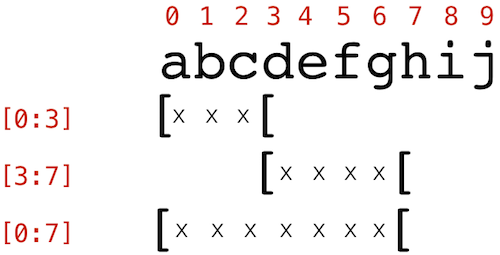
\includegraphics{medias/brackets.png}
\caption{début et fin}
\end{figure}

    \begin{Verbatim}[commandchars=\\\{\}]
{\color{incolor}In [{\color{incolor}3}]:} \PY{c+c1}{\PYZsh{} chaine[a:b] + chaine[b:c] == chaine[a:c]}
        \PY{n}{chaine}\PY{p}{[}\PY{l+m+mi}{0}\PY{p}{:}\PY{l+m+mi}{3}\PY{p}{]} \PY{o}{+} \PY{n}{chaine}\PY{p}{[}\PY{l+m+mi}{3}\PY{p}{:}\PY{l+m+mi}{7}\PY{p}{]} \PY{o}{==} \PY{n}{chaine}\PY{p}{[}\PY{l+m+mi}{0}\PY{p}{:}\PY{l+m+mi}{7}\PY{p}{]}
\end{Verbatim}


\begin{Verbatim}[commandchars=\\\{\}]
{\color{outcolor}Out[{\color{outcolor}3}]:} True
\end{Verbatim}
            
    \hypertarget{bornes-omises}{%
\paragraph{Bornes omises\\\\}\label{bornes-omises}}

    On peut omettre une borne~:

    \begin{Verbatim}[commandchars=\\\{\}]
{\color{incolor}In [{\color{incolor}4}]:} \PY{c+c1}{\PYZsh{} si on omet la première borne, cela signifie que}
        \PY{c+c1}{\PYZsh{} la slice commence au début de l\PYZsq{}objet}
        \PY{n}{chaine}\PY{p}{[}\PY{p}{:}\PY{l+m+mi}{6}\PY{p}{]}
\end{Verbatim}


\begin{Verbatim}[commandchars=\\\{\}]
{\color{outcolor}Out[{\color{outcolor}4}]:} 'abcdef'
\end{Verbatim}
            
    \begin{Verbatim}[commandchars=\\\{\}]
{\color{incolor}In [{\color{incolor}5}]:} \PY{c+c1}{\PYZsh{} et bien entendu c\PYZsq{}est la même chose si on omet la deuxième borne}
        \PY{n}{chaine}\PY{p}{[}\PY{l+m+mi}{24}\PY{p}{:}\PY{p}{]}
\end{Verbatim}


\begin{Verbatim}[commandchars=\\\{\}]
{\color{outcolor}Out[{\color{outcolor}5}]:} 'yz'
\end{Verbatim}
            
    \begin{Verbatim}[commandchars=\\\{\}]
{\color{incolor}In [{\color{incolor}6}]:} \PY{c+c1}{\PYZsh{} ou même omettre les deux bornes, auquel cas on}
        \PY{c+c1}{\PYZsh{} fait une copie de l\PYZsq{}objet \PYZhy{} on y reviendra plus tard}
        \PY{n}{chaine}\PY{p}{[}\PY{p}{:}\PY{p}{]}
\end{Verbatim}


\begin{Verbatim}[commandchars=\\\{\}]
{\color{outcolor}Out[{\color{outcolor}6}]:} 'abcdefghijklmnopqrstuvwxyz'
\end{Verbatim}
            
    \hypertarget{indices-nuxe9gatifs}{%
\paragraph{Indices négatifs\\\\}\label{indices-nuxe9gatifs}}

    On peut utiliser des indices négatifs pour compter à partir de la fin~:

    \begin{Verbatim}[commandchars=\\\{\}]
{\color{incolor}In [{\color{incolor}7}]:} \PY{n}{chaine}\PY{p}{[}\PY{l+m+mi}{3}\PY{p}{:}\PY{o}{\PYZhy{}}\PY{l+m+mi}{3}\PY{p}{]}
\end{Verbatim}


\begin{Verbatim}[commandchars=\\\{\}]
{\color{outcolor}Out[{\color{outcolor}7}]:} 'defghijklmnopqrstuvw'
\end{Verbatim}
            
    \begin{Verbatim}[commandchars=\\\{\}]
{\color{incolor}In [{\color{incolor}8}]:} \PY{n}{chaine}\PY{p}{[}\PY{o}{\PYZhy{}}\PY{l+m+mi}{3}\PY{p}{:}\PY{p}{]}
\end{Verbatim}


\begin{Verbatim}[commandchars=\\\{\}]
{\color{outcolor}Out[{\color{outcolor}8}]:} 'xyz'
\end{Verbatim}
            
    \hypertarget{slice-avec-pas}{%
\subsubsection{Slice avec pas}\label{slice-avec-pas}}

    Il est également possible de préciser un \emph{pas}, de façon à ne
choisir par exemple, dans la plage donnée, qu'un élément sur deux~:

    \begin{Verbatim}[commandchars=\\\{\}]
{\color{incolor}In [{\color{incolor}9}]:} \PY{c+c1}{\PYZsh{} le pas est précisé après un deuxième deux\PYZhy{}points (:)}
        \PY{c+c1}{\PYZsh{} ici on va choisir un caractère sur deux dans la plage [3:\PYZhy{}3]}
        \PY{n}{chaine}\PY{p}{[}\PY{l+m+mi}{3}\PY{p}{:}\PY{o}{\PYZhy{}}\PY{l+m+mi}{3}\PY{p}{:}\PY{l+m+mi}{2}\PY{p}{]}
\end{Verbatim}


\begin{Verbatim}[commandchars=\\\{\}]
{\color{outcolor}Out[{\color{outcolor}9}]:} 'dfhjlnprtv'
\end{Verbatim}
            
    Comme on le devine, le troisième élément de la slice, ici \texttt{2},
détermine le pas. On ne retient donc, dans la chaîne \texttt{defghi...}
que \texttt{d}, puis \texttt{f}, et ainsi de suite.\\

On peut préciser du coup la borne de fin (ici \texttt{-3}) avec un peu
de liberté, puisqu'ici on obtiendrait un résultat identique avec
\texttt{-4}.

    \begin{Verbatim}[commandchars=\\\{\}]
{\color{incolor}In [{\color{incolor}10}]:} \PY{n}{chaine}\PY{p}{[}\PY{l+m+mi}{3}\PY{p}{:}\PY{o}{\PYZhy{}}\PY{l+m+mi}{4}\PY{p}{:}\PY{l+m+mi}{2}\PY{p}{]}
\end{Verbatim}


\begin{Verbatim}[commandchars=\\\{\}]
{\color{outcolor}Out[{\color{outcolor}10}]:} 'dfhjlnprtv'
\end{Verbatim}
            
    \hypertarget{pas-nuxe9gatif}{%
\subsubsection{Pas négatif}\label{pas-nuxe9gatif}}

    Il est même possible de spécifier un pas négatif. Dans ce cas, de
manière un peu contre-intuitive, il faut préciser un début (le premier
indice de la slice) qui soit \emph{plus à droite} que la fin (le second
indice).\\

Pour prendre un exemple, comme l'élément d'indice \texttt{-3},
c'est-à-dire \texttt{x}, est plus à droite que l'élément d'indice
\texttt{3}, c'est-à-dire \texttt{d}, évidemment si on ne précisait pas
le pas (qui revient à choisir un pas égal à \texttt{1}), on obtiendrait
une liste vide~:

    \begin{Verbatim}[commandchars=\\\{\}]
{\color{incolor}In [{\color{incolor}11}]:} \PY{n}{chaine}\PY{p}{[}\PY{o}{\PYZhy{}}\PY{l+m+mi}{3}\PY{p}{:}\PY{l+m+mi}{3}\PY{p}{]}
\end{Verbatim}


\begin{Verbatim}[commandchars=\\\{\}]
{\color{outcolor}Out[{\color{outcolor}11}]:} ''
\end{Verbatim}
            
    Si maintenant on précise un pas négatif, on obtient cette fois~:

    \begin{Verbatim}[commandchars=\\\{\}]
{\color{incolor}In [{\color{incolor}12}]:} \PY{n}{chaine}\PY{p}{[}\PY{o}{\PYZhy{}}\PY{l+m+mi}{3}\PY{p}{:}\PY{l+m+mi}{3}\PY{p}{:}\PY{o}{\PYZhy{}}\PY{l+m+mi}{2}\PY{p}{]}
\end{Verbatim}


\begin{Verbatim}[commandchars=\\\{\}]
{\color{outcolor}Out[{\color{outcolor}12}]:} 'xvtrpnljhf'
\end{Verbatim}
            
    \hypertarget{conclusion}{%
\subsubsection{Conclusion}\label{conclusion}}

    À nouveau, souvenez-vous que tous ces mécanismes fonctionnent avec de
nombreux autres types que les chaînes de caractères. En voici deux
exemples qui anticipent tous les deux sur la suite, mais qui devraient
illustrer les vastes possibilités qui sont offertes avec les slices.

    \hypertarget{listes}{%
\paragraph{Listes}\label{listes}}

    Par exemple sur les listes~:

    \begin{Verbatim}[commandchars=\\\{\}]
{\color{incolor}In [{\color{incolor}13}]:} \PY{n}{liste} \PY{o}{=} \PY{p}{[}\PY{l+m+mi}{0}\PY{p}{,} \PY{l+m+mi}{2}\PY{p}{,} \PY{l+m+mi}{4}\PY{p}{,} \PY{l+m+mi}{8}\PY{p}{,} \PY{l+m+mi}{16}\PY{p}{,} \PY{l+m+mi}{32}\PY{p}{,} \PY{l+m+mi}{64}\PY{p}{,} \PY{l+m+mi}{128}\PY{p}{]}
         \PY{n}{liste}
\end{Verbatim}


\begin{Verbatim}[commandchars=\\\{\}]
{\color{outcolor}Out[{\color{outcolor}13}]:} [0, 2, 4, 8, 16, 32, 64, 128]
\end{Verbatim}
            
    \begin{Verbatim}[commandchars=\\\{\}]
{\color{incolor}In [{\color{incolor}14}]:} \PY{n}{liste}\PY{p}{[}\PY{o}{\PYZhy{}}\PY{l+m+mi}{1}\PY{p}{:}\PY{l+m+mi}{1}\PY{p}{:}\PY{o}{\PYZhy{}}\PY{l+m+mi}{2}\PY{p}{]}
\end{Verbatim}


\begin{Verbatim}[commandchars=\\\{\}]
{\color{outcolor}Out[{\color{outcolor}14}]:} [128, 32, 8]
\end{Verbatim}
            
    Et même ceci, qui peut être déroutant. Nous reviendrons dessus.

    \begin{Verbatim}[commandchars=\\\{\}]
{\color{incolor}In [{\color{incolor}15}]:} \PY{n}{liste}\PY{p}{[}\PY{l+m+mi}{2}\PY{p}{:}\PY{l+m+mi}{4}\PY{p}{]} \PY{o}{=} \PY{p}{[}\PY{l+m+mi}{100}\PY{p}{,} \PY{l+m+mi}{200}\PY{p}{,} \PY{l+m+mi}{300}\PY{p}{,} \PY{l+m+mi}{400}\PY{p}{,} \PY{l+m+mi}{500}\PY{p}{]}
         \PY{n}{liste}
\end{Verbatim}


\begin{Verbatim}[commandchars=\\\{\}]
{\color{outcolor}Out[{\color{outcolor}15}]:} [0, 2, 100, 200, 300, 400, 500, 16, 32, 64, 128]
\end{Verbatim}
            
    \hypertarget{compluxe9ment---niveau-avancuxe9}{%
\subsection{Complément - niveau
avancé}\label{compluxe9ment---niveau-avancuxe9}}

    \hypertarget{numpy}{%
\paragraph{\texorpdfstring{\texttt{numpy}}{numpy}}\label{numpy}}

    La bibliothèque \texttt{numpy} permet de manipuler des tableaux ou des
matrices. En anticipant (beaucoup) sur son usage que nous reverrons bien
entendu en détail, voici un aperçu de ce que l'on peut faire avec des
slices sur des objets \texttt{numpy}~:

    \begin{Verbatim}[commandchars=\\\{\}]
{\color{incolor}In [{\color{incolor}16}]:} \PY{c+c1}{\PYZsh{} ces deux premières cellules sont à admettre}
         \PY{c+c1}{\PYZsh{} on construit un tableau ligne}
         \PY{k+kn}{import} \PY{n+nn}{numpy} \PY{k}{as} \PY{n+nn}{np}
         
         \PY{n}{un\PYZus{}cinq} \PY{o}{=} \PY{n}{np}\PY{o}{.}\PY{n}{array}\PY{p}{(}\PY{p}{[}\PY{l+m+mi}{1}\PY{p}{,} \PY{l+m+mi}{2}\PY{p}{,} \PY{l+m+mi}{3}\PY{p}{,} \PY{l+m+mi}{4}\PY{p}{,} \PY{l+m+mi}{5}\PY{p}{]}\PY{p}{)}
         \PY{n}{un\PYZus{}cinq}
\end{Verbatim}


\begin{Verbatim}[commandchars=\\\{\}]
{\color{outcolor}Out[{\color{outcolor}16}]:} array([1, 2, 3, 4, 5])
\end{Verbatim}
            
    \begin{Verbatim}[commandchars=\\\{\}]
{\color{incolor}In [{\color{incolor}17}]:} \PY{c+c1}{\PYZsh{} ces deux premières cellules sont à admettre}
         \PY{c+c1}{\PYZsh{} on le combine avec lui\PYZhy{}même \PYZhy{} et en utilisant une slice un peu magique}
         \PY{c+c1}{\PYZsh{} pour former un tableau carré 5x5}
         
         \PY{n}{array} \PY{o}{=} \PY{l+m+mi}{10} \PY{o}{*} \PY{n}{un\PYZus{}cinq}\PY{p}{[}\PY{p}{:}\PY{p}{,} \PY{n}{np}\PY{o}{.}\PY{n}{newaxis}\PY{p}{]} \PY{o}{+} \PY{n}{un\PYZus{}cinq}
         \PY{n}{array}
\end{Verbatim}


\begin{Verbatim}[commandchars=\\\{\}]
{\color{outcolor}Out[{\color{outcolor}17}]:} array([[11, 12, 13, 14, 15],
                [21, 22, 23, 24, 25],
                [31, 32, 33, 34, 35],
                [41, 42, 43, 44, 45],
                [51, 52, 53, 54, 55]])
\end{Verbatim}
            
    Sur ce tableau de taille 5x5, nous pouvons aussi faire du slicing et
extraire le sous-tableau 3x3 au centre~:

    \begin{Verbatim}[commandchars=\\\{\}]
{\color{incolor}In [{\color{incolor}18}]:} \PY{n}{centre} \PY{o}{=} \PY{n}{array}\PY{p}{[}\PY{l+m+mi}{1}\PY{p}{:}\PY{l+m+mi}{4}\PY{p}{,} \PY{l+m+mi}{1}\PY{p}{:}\PY{l+m+mi}{4}\PY{p}{]}
         \PY{n}{centre}
\end{Verbatim}


\begin{Verbatim}[commandchars=\\\{\}]
{\color{outcolor}Out[{\color{outcolor}18}]:} array([[22, 23, 24],
                [32, 33, 34],
                [42, 43, 44]])
\end{Verbatim}
            
    On peut bien sûr également utiliser un pas~:

    \begin{Verbatim}[commandchars=\\\{\}]
{\color{incolor}In [{\color{incolor}19}]:} \PY{n}{coins} \PY{o}{=} \PY{n}{array}\PY{p}{[}\PY{p}{:}\PY{p}{:}\PY{l+m+mi}{4}\PY{p}{,} \PY{p}{:}\PY{p}{:}\PY{l+m+mi}{4}\PY{p}{]}
         \PY{n}{coins}
\end{Verbatim}


\begin{Verbatim}[commandchars=\\\{\}]
{\color{outcolor}Out[{\color{outcolor}19}]:} array([[11, 15],
                [51, 55]])
\end{Verbatim}
            
    Ou bien retourner complètement dans une direction~:

    \begin{Verbatim}[commandchars=\\\{\}]
{\color{incolor}In [{\color{incolor}20}]:} \PY{n}{tete\PYZus{}en\PYZus{}bas} \PY{o}{=} \PY{n}{array}\PY{p}{[}\PY{p}{:}\PY{p}{:}\PY{o}{\PYZhy{}}\PY{l+m+mi}{1}\PY{p}{,}\PY{p}{:}\PY{p}{]}
         \PY{n}{tete\PYZus{}en\PYZus{}bas}
\end{Verbatim}


\begin{Verbatim}[commandchars=\\\{\}]
{\color{outcolor}Out[{\color{outcolor}20}]:} array([[51, 52, 53, 54, 55],
                [41, 42, 43, 44, 45],
                [31, 32, 33, 34, 35],
                [21, 22, 23, 24, 25],
                [11, 12, 13, 14, 15]])
\end{Verbatim}
        \hypertarget{muxe9thodes-spuxe9cifiques-aux-listes}{%
\section{Méthodes spécifiques aux
listes}\label{muxe9thodes-spuxe9cifiques-aux-listes}}

    \hypertarget{compluxe9ment---niveau-basique}{%
\subsection{Complément - niveau
basique}\label{compluxe9ment---niveau-basique}}

    Voici quelques unes des méthodes disponibles sur le type \texttt{list}.

    \hypertarget{trouver-linformation}{%
\subsubsection{Trouver l'information}\label{trouver-linformation}}

    Pour commencer, rappelons comment retrouver la liste des méthodes
définies sur le type \texttt{list}~:

    \begin{Verbatim}[commandchars=\\\{\}]
{\color{incolor}In [{\color{incolor}1}]:} \PY{n}{help}\PY{p}{(}\PY{n+nb}{list}\PY{p}{)}
\end{Verbatim}


    \begin{Verbatim}[commandchars=\\\{\}]
Help on class list in module builtins:

class list(object)
 |  list() -> new empty list
 |  list(iterable) -> new list initialized from iterable's items
 |  
 |  Methods defined here:
 |  
 |  \_\_add\_\_(self, value, /)
 |      Return self+value.
 |  
 |  \_\_contains\_\_(self, key, /)
 |      Return key in self.
 |  
 |  \_\_delitem\_\_(self, key, /)
 |      Delete self[key].
 |  
 |  \_\_eq\_\_(self, value, /)
 |      Return self==value.
 |  
 |  \_\_ge\_\_(self, value, /)
 |      Return self>=value.
 |  
 |  \_\_getattribute\_\_(self, name, /)
 |      Return getattr(self, name).
 |  
 |  \_\_getitem\_\_({\ldots})
 |      x.\_\_getitem\_\_(y) <==> x[y]
 |  
 |  \_\_gt\_\_(self, value, /)
 |      Return self>value.
 |  
 |  \_\_iadd\_\_(self, value, /)
 |      Implement self+=value.
 |  
 |  \_\_imul\_\_(self, value, /)
 |      Implement self*=value.
 |  
 |  \_\_init\_\_(self, /, *args, **kwargs)
 |      Initialize self.  See help(type(self)) for accurate signature.
 |  
 |  \_\_iter\_\_(self, /)
 |      Implement iter(self).
 |  
 |  \_\_le\_\_(self, value, /)
 |      Return self<=value.
 |  
 |  \_\_len\_\_(self, /)
 |      Return len(self).
 |  
 |  \_\_lt\_\_(self, value, /)
 |      Return self<value.
 |  
 |  \_\_mul\_\_(self, value, /)
 |      Return self*value.n
 |  
 |  \_\_ne\_\_(self, value, /)
 |      Return self!=value.
 |  
 |  \_\_new\_\_(*args, **kwargs) from builtins.type
 |      Create and return a new object.  See help(type) for accurate signature.
 |  
 |  \_\_repr\_\_(self, /)
 |      Return repr(self).
 |  
 |  \_\_reversed\_\_({\ldots})
 |      L.\_\_reversed\_\_() -- return a reverse iterator over the list
 |  
 |  \_\_rmul\_\_(self, value, /)
 |      Return self*value.
 |  
 |  \_\_setitem\_\_(self, key, value, /)
 |      Set self[key] to value.
 |  
 |  \_\_sizeof\_\_({\ldots})
 |      L.\_\_sizeof\_\_() -- size of L in memory, in bytes
 |  
 |  append({\ldots})
 |      L.append(object) -> None -- append object to end
 |  
 |  clear({\ldots})
 |      L.clear() -> None -- remove all items from L
 |  
 |  copy({\ldots})
 |      L.copy() -> list -- a shallow copy of L
 |  
 |  count({\ldots})
 |      L.count(value) -> integer -- return number of occurrences of value
 |  
 |  extend({\ldots})
 |      L.extend(iterable) -> None -- extend list by appending elements from the iterable
 |  
 |  index({\ldots})
 |      L.index(value, [start, [stop]]) -> integer -- return first index of value.
 |      Raises ValueError if the value is not present.
 |  
 |  insert({\ldots})
 |      L.insert(index, object) -- insert object before index
 |  
 |  pop({\ldots})
 |      L.pop([index]) -> item -- remove and return item at index (default last).
 |      Raises IndexError if list is empty or index is out of range.
 |  
 |  remove({\ldots})
 |      L.remove(value) -> None -- remove first occurrence of value.
 |      Raises ValueError if the value is not present.
 |  
 |  reverse({\ldots})
 |      L.reverse() -- reverse *IN PLACE*
 |  
 |  sort({\ldots})
 |      L.sort(key=None, reverse=False) -> None -- stable sort *IN PLACE*
 |  
 |  ----------------------------------------------------------------------
 |  Data and other attributes defined here:
 |  
 |  \_\_hash\_\_ = None


    \end{Verbatim}

    Ignorez les méthodes dont le nom commence et termine par \texttt{\_\_}
(nous parlerons de ceci en semaine 6), vous trouvez alors les méthodes
utiles listées entre \texttt{append} et \texttt{sort}.\\

Certaines de ces méthodes ont été vues dans la vidéo sur les séquences,
c'est le cas notamment de \texttt{count} et \texttt{index}.\\

    Nous allons à présent décrire les autres, partiellement et brièvement.
Un autre complément décrit la méthode \texttt{sort}. Reportez-vous au
lien donné en fin de notebook pour obtenir une information plus
complète.\\

    Donnons-nous pour commencer une liste témoin~:

    \begin{Verbatim}[commandchars=\\\{\}]
{\color{incolor}In [{\color{incolor}2}]:} \PY{n}{liste} \PY{o}{=} \PY{p}{[}\PY{l+m+mi}{0}\PY{p}{,} \PY{l+m+mi}{1}\PY{p}{,} \PY{l+m+mi}{2}\PY{p}{,} \PY{l+m+mi}{3}\PY{p}{]}
        \PY{n+nb}{print}\PY{p}{(}\PY{l+s+s1}{\PYZsq{}}\PY{l+s+s1}{liste}\PY{l+s+s1}{\PYZsq{}}\PY{p}{,} \PY{n}{liste}\PY{p}{)}
\end{Verbatim}


    \begin{Verbatim}[commandchars=\\\{\}]
liste [0, 1, 2, 3]

    \end{Verbatim}

    \textbf{Avertissements}~:

\begin{itemize}
\tightlist
\item
  soyez bien attentifs au nombre de fois où vous exécutez les cellules
  de ce notebook~;
\item
  par exemple une liste renversée deux fois peut donner l'impression que
  \texttt{reverse} ne marche pas~;
\item
  n'hésitez pas à utiliser le menu \emph{Cell~-\textgreater{}~Run~All}
  pour réexécuter en une seule fois le notebook entier.
\end{itemize}

    \hypertarget{append}{%
\subsubsection{\texorpdfstring{\textbf{append}}{append}}\label{append}}

    La méthode \texttt{append} permet d'ajouter \textbf{un élément} à la fin
d'une liste~:

    \begin{Verbatim}[commandchars=\\\{\}]
{\color{incolor}In [{\color{incolor}3}]:} \PY{n}{liste}\PY{o}{.}\PY{n}{append}\PY{p}{(}\PY{l+s+s1}{\PYZsq{}}\PY{l+s+s1}{ap}\PY{l+s+s1}{\PYZsq{}}\PY{p}{)}
        \PY{n+nb}{print}\PY{p}{(}\PY{l+s+s1}{\PYZsq{}}\PY{l+s+s1}{liste}\PY{l+s+s1}{\PYZsq{}}\PY{p}{,} \PY{n}{liste}\PY{p}{)}
\end{Verbatim}


    \begin{Verbatim}[commandchars=\\\{\}]
liste [0, 1, 2, 3, 'ap']

    \end{Verbatim}

    \hypertarget{extend}{%
\subsubsection{\texorpdfstring{\textbf{extend}}{extend}}\label{extend}}

    La méthode \texttt{extend} réalise la même opération, mais avec
\textbf{tous les éléments} de la liste qu'on lui passe en argument~:

    \begin{Verbatim}[commandchars=\\\{\}]
{\color{incolor}In [{\color{incolor}4}]:} \PY{n}{liste2} \PY{o}{=} \PY{p}{[}\PY{l+s+s1}{\PYZsq{}}\PY{l+s+s1}{ex1}\PY{l+s+s1}{\PYZsq{}}\PY{p}{,} \PY{l+s+s1}{\PYZsq{}}\PY{l+s+s1}{ex2}\PY{l+s+s1}{\PYZsq{}}\PY{p}{]}
        \PY{n}{liste}\PY{o}{.}\PY{n}{extend}\PY{p}{(}\PY{n}{liste2}\PY{p}{)}
        \PY{n+nb}{print}\PY{p}{(}\PY{l+s+s1}{\PYZsq{}}\PY{l+s+s1}{liste}\PY{l+s+s1}{\PYZsq{}}\PY{p}{,} \PY{n}{liste}\PY{p}{)}
\end{Verbatim}


    \begin{Verbatim}[commandchars=\\\{\}]
liste [0, 1, 2, 3, 'ap', 'ex1', 'ex2']

    \end{Verbatim}

    \hypertarget{append-vs}{%
\subsubsection{\texorpdfstring{\textbf{append} \emph{vs}
\textbf{+}}{append vs +}}\label{append-vs}}

    Ces deux méthodes \texttt{append} et \texttt{extend} sont donc assez
voisines~; avant de voir d'autres méthodes de \texttt{list}, prenons un
peu le temps de comparer leur comportement avec l'addition \texttt{+} de
liste. L'élément clé ici, on l'a déjà vu dans la vidéo, est que la liste
est un objet \textbf{mutable}. \texttt{append} et \texttt{extend}
\textbf{modifient} la liste sur laquelle elles travaillent, alors que
l'addition \textbf{crée un nouvel objet}.

    \begin{Verbatim}[commandchars=\\\{\}]
{\color{incolor}In [{\color{incolor}5}]:} \PY{c+c1}{\PYZsh{} pour créer une liste avec les n premiers entiers, on utilise}
        \PY{c+c1}{\PYZsh{} la fonction built\PYZhy{}in range(), que l\PYZsq{}on convertit en liste}
        \PY{c+c1}{\PYZsh{} on aura l\PYZsq{}occasion d\PYZsq{}y revenir}
        \PY{n}{a1} \PY{o}{=} \PY{n+nb}{list}\PY{p}{(}\PY{n+nb}{range}\PY{p}{(}\PY{l+m+mi}{3}\PY{p}{)}\PY{p}{)}
        \PY{n+nb}{print}\PY{p}{(}\PY{n}{a1}\PY{p}{)}
\end{Verbatim}


    \begin{Verbatim}[commandchars=\\\{\}]
[0, 1, 2]

    \end{Verbatim}

    \begin{Verbatim}[commandchars=\\\{\}]
{\color{incolor}In [{\color{incolor}6}]:} \PY{n}{a2} \PY{o}{=} \PY{n+nb}{list}\PY{p}{(}\PY{n+nb}{range}\PY{p}{(}\PY{l+m+mi}{10}\PY{p}{,} \PY{l+m+mi}{13}\PY{p}{)}\PY{p}{)}
        \PY{n+nb}{print}\PY{p}{(}\PY{n}{a2}\PY{p}{)}
\end{Verbatim}


    \begin{Verbatim}[commandchars=\\\{\}]
[10, 11, 12]

    \end{Verbatim}

    \begin{Verbatim}[commandchars=\\\{\}]
{\color{incolor}In [{\color{incolor}7}]:} \PY{c+c1}{\PYZsh{} le fait d\PYZsq{}utiliser + crée une nouvelle liste}
        \PY{n}{a3} \PY{o}{=} \PY{n}{a1} \PY{o}{+} \PY{n}{a2}
\end{Verbatim}


    \begin{Verbatim}[commandchars=\\\{\}]
{\color{incolor}In [{\color{incolor}8}]:} \PY{c+c1}{\PYZsh{} si bien que maintenant on a trois objets différents}
        \PY{n+nb}{print}\PY{p}{(}\PY{l+s+s1}{\PYZsq{}}\PY{l+s+s1}{a1}\PY{l+s+s1}{\PYZsq{}}\PY{p}{,} \PY{n}{a1}\PY{p}{)}
        \PY{n+nb}{print}\PY{p}{(}\PY{l+s+s1}{\PYZsq{}}\PY{l+s+s1}{a2}\PY{l+s+s1}{\PYZsq{}}\PY{p}{,} \PY{n}{a2}\PY{p}{)}
        \PY{n+nb}{print}\PY{p}{(}\PY{l+s+s1}{\PYZsq{}}\PY{l+s+s1}{a3}\PY{l+s+s1}{\PYZsq{}}\PY{p}{,} \PY{n}{a3}\PY{p}{)}
\end{Verbatim}


    \begin{Verbatim}[commandchars=\\\{\}]
a1 [0, 1, 2]
a2 [10, 11, 12]
a3 [0, 1, 2, 10, 11, 12]

    \end{Verbatim}

    Comme on le voit, après une addition, les deux termes de l'addition sont
inchangés. Pour bien comprendre, voyons exactement le même scénario sous
pythontutor~:

    \begin{Verbatim}[commandchars=\\\{\}]
{\color{incolor}In [{\color{incolor} }]:} \PY{o}{\PYZpc{}}\PY{k}{load\PYZus{}ext} ipythontutor
\end{Verbatim}


    \textbf{Note}~: une fois que vous avez évalué la cellule avec
\texttt{\%\%ipythontutor}, vous devez cliquer sur le bouton
\texttt{Forward} pour voir pas à pas le comportement du programme.

    \begin{Verbatim}[commandchars=\\\{\}]
{\color{incolor}In [{\color{incolor} }]:} \PY{o}{\PYZpc{}\PYZpc{}}\PY{k}{ipythontutor} height=230 ratio=0.7
        a1 = list(range(3))
        a2 = list(range(10, 13))
        a3 = a1 + a2
\end{Verbatim}


    Alors que si on avait utilisé \texttt{extend}, on aurait obtenu ceci~:

    \begin{Verbatim}[commandchars=\\\{\}]
{\color{incolor}In [{\color{incolor} }]:} \PY{o}{\PYZpc{}\PYZpc{}}\PY{k}{ipythontutor} height=200 ratio=0.75
        e1 = list(range(3))
        e2 = list(range(10, 13))
        e3 = e1.extend(e2)
\end{Verbatim}


    Ici on tire profit du fait que la liste est un objet mutable~:
\texttt{extend} \textbf{modifie} l'objet sur lequel on l'appelle (ici
\texttt{e1}). Dans ce scénario on ne crée en tout que deux objets, et du
coup il est inutile pour extend de renvoyer quoi que ce soit, et c'est
pourquoi \texttt{e3} ici vaut None.\\

    C'est pour cette raison que~:

\begin{itemize}
\tightlist
\item
  l'addition est disponible sur tous les types séquences - on peut
  toujours réaliser l'addition puisqu'on crée un nouvel objet pour
  stocker le résultat de l'addition~;
\item
  mais \texttt{append} et \texttt{extend} ne sont par exemple
  \textbf{pas disponibles} sur les chaînes de caractères, qui sont
  \textbf{immuables} - si \texttt{e1} était une chaîne, on ne pourrait
  pas la modifier pour lui ajouter des éléments.
\end{itemize}

    \hypertarget{insert}{%
\subsubsection{\texorpdfstring{\textbf{insert}}{insert}}\label{insert}}

    Reprenons notre inventaire des méthodes de \texttt{list}, et pour cela
rappelons nous le contenu de la variable \texttt{liste}~:

    \begin{Verbatim}[commandchars=\\\{\}]
{\color{incolor}In [{\color{incolor}9}]:} \PY{n}{liste}
\end{Verbatim}


\begin{Verbatim}[commandchars=\\\{\}]
{\color{outcolor}Out[{\color{outcolor}9}]:} [0, 1, 2, 3, 'ap', 'ex1', 'ex2']
\end{Verbatim}
            
    La méthode \texttt{insert} permet, comme le nom le suggère, d'insérer un
élément à une certaine position~; comme toujours les indices commencent
à zéro et donc~:

    \begin{Verbatim}[commandchars=\\\{\}]
{\color{incolor}In [{\color{incolor}10}]:} \PY{c+c1}{\PYZsh{} insérer à l\PYZsq{}index 2}
         \PY{n}{liste}\PY{o}{.}\PY{n}{insert}\PY{p}{(}\PY{l+m+mi}{2}\PY{p}{,} \PY{l+s+s1}{\PYZsq{}}\PY{l+s+s1}{1 bis}\PY{l+s+s1}{\PYZsq{}}\PY{p}{)}
         \PY{n+nb}{print}\PY{p}{(}\PY{l+s+s1}{\PYZsq{}}\PY{l+s+s1}{liste}\PY{l+s+s1}{\PYZsq{}}\PY{p}{,} \PY{n}{liste}\PY{p}{)}
\end{Verbatim}


    \begin{Verbatim}[commandchars=\\\{\}]
liste [0, 1, '1 bis', 2, 3, 'ap', 'ex1', 'ex2']

    \end{Verbatim}

    On peut remarquer qu'un résultat analogue peut être obtenu avec une
affectation de slice~; par exemple pour insérer au rang 5 (i.e.~avant
\texttt{ap}), on pourrait aussi bien faire~:

    \begin{Verbatim}[commandchars=\\\{\}]
{\color{incolor}In [{\color{incolor}11}]:} \PY{n}{liste}\PY{p}{[}\PY{l+m+mi}{5}\PY{p}{:}\PY{l+m+mi}{5}\PY{p}{]} \PY{o}{=} \PY{p}{[}\PY{l+s+s1}{\PYZsq{}}\PY{l+s+s1}{3 bis}\PY{l+s+s1}{\PYZsq{}}\PY{p}{]}
         \PY{n+nb}{print}\PY{p}{(}\PY{l+s+s1}{\PYZsq{}}\PY{l+s+s1}{liste}\PY{l+s+s1}{\PYZsq{}}\PY{p}{,} \PY{n}{liste}\PY{p}{)}
\end{Verbatim}


    \begin{Verbatim}[commandchars=\\\{\}]
liste [0, 1, '1 bis', 2, 3, '3 bis', 'ap', 'ex1', 'ex2']

    \end{Verbatim}

    \hypertarget{remove}{%
\subsubsection{\texorpdfstring{\textbf{remove}}{remove}}\label{remove}}

    La méthode \texttt{remove} détruit la \textbf{première occurrence} d'un
objet dans la liste~:

    \begin{Verbatim}[commandchars=\\\{\}]
{\color{incolor}In [{\color{incolor}12}]:} \PY{n}{liste}\PY{o}{.}\PY{n}{remove}\PY{p}{(}\PY{l+m+mi}{3}\PY{p}{)}
         \PY{n+nb}{print}\PY{p}{(}\PY{l+s+s1}{\PYZsq{}}\PY{l+s+s1}{liste}\PY{l+s+s1}{\PYZsq{}}\PY{p}{,} \PY{n}{liste}\PY{p}{)}
\end{Verbatim}


    \begin{Verbatim}[commandchars=\\\{\}]
liste [0, 1, '1 bis', 2, '3 bis', 'ap', 'ex1', 'ex2']

    \end{Verbatim}

    \hypertarget{pop}{%
\subsubsection{\texorpdfstring{\textbf{pop}}{pop}}\label{pop}}

    La méthode \texttt{pop} prend en argument un indice~; elle permet
d'extraire l'élément à cet indice. En un seul appel on obtient la valeur
de l'élément et on l'enlève de la liste~:

    \begin{Verbatim}[commandchars=\\\{\}]
{\color{incolor}In [{\color{incolor}13}]:} \PY{n}{popped} \PY{o}{=} \PY{n}{liste}\PY{o}{.}\PY{n}{pop}\PY{p}{(}\PY{l+m+mi}{0}\PY{p}{)}
         \PY{n+nb}{print}\PY{p}{(}\PY{l+s+s1}{\PYZsq{}}\PY{l+s+s1}{popped}\PY{l+s+s1}{\PYZsq{}}\PY{p}{,} \PY{n}{popped}\PY{p}{,} \PY{l+s+s1}{\PYZsq{}}\PY{l+s+s1}{liste}\PY{l+s+s1}{\PYZsq{}}\PY{p}{,} \PY{n}{liste}\PY{p}{)}
\end{Verbatim}


    \begin{Verbatim}[commandchars=\\\{\}]
popped 0 liste [1, '1 bis', 2, '3 bis', 'ap', 'ex1', 'ex2']

    \end{Verbatim}

    Si l'indice n'est pas précisé, c'est le dernier élément de la liste qui
est visé~:

    \begin{Verbatim}[commandchars=\\\{\}]
{\color{incolor}In [{\color{incolor}14}]:} \PY{n}{popped} \PY{o}{=} \PY{n}{liste}\PY{o}{.}\PY{n}{pop}\PY{p}{(}\PY{p}{)}
         \PY{n+nb}{print}\PY{p}{(}\PY{l+s+s1}{\PYZsq{}}\PY{l+s+s1}{popped}\PY{l+s+s1}{\PYZsq{}}\PY{p}{,} \PY{n}{popped}\PY{p}{,} \PY{l+s+s1}{\PYZsq{}}\PY{l+s+s1}{liste}\PY{l+s+s1}{\PYZsq{}}\PY{p}{,} \PY{n}{liste}\PY{p}{)}
\end{Verbatim}


    \begin{Verbatim}[commandchars=\\\{\}]
popped ex2 liste [1, '1 bis', 2, '3 bis', 'ap', 'ex1']

    \end{Verbatim}

    \hypertarget{reverse}{%
\subsubsection{\texorpdfstring{\textbf{reverse}}{reverse}}\label{reverse}}

    Enfin \texttt{reverse} renverse la liste, le premier élément devient le
dernier~:

    \begin{Verbatim}[commandchars=\\\{\}]
{\color{incolor}In [{\color{incolor}15}]:} \PY{n}{liste}\PY{o}{.}\PY{n}{reverse}\PY{p}{(}\PY{p}{)}
         \PY{n+nb}{print}\PY{p}{(}\PY{l+s+s1}{\PYZsq{}}\PY{l+s+s1}{liste}\PY{l+s+s1}{\PYZsq{}}\PY{p}{,} \PY{n}{liste}\PY{p}{)}
\end{Verbatim}


    \begin{Verbatim}[commandchars=\\\{\}]
liste ['ex1', 'ap', '3 bis', 2, '1 bis', 1]

    \end{Verbatim}

    On peut remarquer ici que le résultat se rapproche de ce qu'on peut
obtenir avec une opération de slicing comme ceci~:

    \begin{Verbatim}[commandchars=\\\{\}]
{\color{incolor}In [{\color{incolor}16}]:} \PY{n}{liste2} \PY{o}{=} \PY{n}{liste}\PY{p}{[}\PY{p}{:}\PY{p}{:}\PY{o}{\PYZhy{}}\PY{l+m+mi}{1}\PY{p}{]}
         \PY{n+nb}{print}\PY{p}{(}\PY{l+s+s1}{\PYZsq{}}\PY{l+s+s1}{liste2}\PY{l+s+s1}{\PYZsq{}}\PY{p}{,} \PY{n}{liste2}\PY{p}{)}
\end{Verbatim}


    \begin{Verbatim}[commandchars=\\\{\}]
liste2 [1, '1 bis', 2, '3 bis', 'ap', 'ex1']

    \end{Verbatim}

    \textbf{À la différence toutefois} qu'avec le slicing c'est une copie de
la liste initiale qui est retournée, la liste de départ quant à elle
n'est pas modifiée.

    \hypertarget{pour-en-savoir-plus}{%
\subsubsection{Pour en savoir plus}\label{pour-en-savoir-plus}}

    \href{https://docs.python.org/3/tutorial/datastructures.html\#more-on-lists}{https://docs.python.org/3/tutorial/datastructures.html\#more-on-lists}

    \hypertarget{note-spuxe9cifique-aux-notebooks}{%
\subsubsection{Note spécifique aux
notebooks}\label{note-spuxe9cifique-aux-notebooks}}

    \hypertarget{help-avec}{%
\paragraph{\texorpdfstring{\texttt{help} avec
\texttt{?}}{help avec ?}}\label{help-avec}}

    Je vous signale en passant que dans un notebook vous pouvez obtenir de
l'aide avec un point d'interrogation \texttt{?} inséré avant ou après un
symbole. Par exemple pour obtenir des précisions sur la méthode
\texttt{list.pop}, on peut faire soit~:

    \begin{Verbatim}[commandchars=\\\{\}]
{\color{incolor}In [{\color{incolor}17}]:} \PY{c+c1}{\PYZsh{} fonctionne dans tous les environnements Python}
         \PY{n}{help}\PY{p}{(}\PY{n+nb}{list}\PY{o}{.}\PY{n}{pop}\PY{p}{)}
\end{Verbatim}


    \begin{Verbatim}[commandchars=\\\{\}]
Help on method\_descriptor:

pop({\ldots})
    L.pop([index]) -> item -- remove and return item at index (default last).
    Raises IndexError if list is empty or index is out of range.


    \end{Verbatim}

    \begin{Verbatim}[commandchars=\\\{\}]
{\color{incolor}In [{\color{incolor}18}]:} \PY{c+c1}{\PYZsh{} spécifique aux notebooks}
         \PY{c+c1}{\PYZsh{} l\PYZsq{}affichage obtenu est légèrement différent}
         \PY{c+c1}{\PYZsh{} tapez la touche \PYZsq{}Esc\PYZsq{} \PYZhy{} ou cliquez la petite croix}
         \PY{c+c1}{\PYZsh{} pour faire disparaitre le dialogue qui apparaît en bas}
         list.pop\PY{o}{?}
\end{Verbatim}


    \hypertarget{compluxe9tion-avec-tab}{%
\paragraph{\texorpdfstring{Complétion avec
\texttt{Tab}}{Complétion avec Tab}\\\\}\label{compluxe9tion-avec-tab}}

    Dans un notebook vous avez aussi la complétion~; si vous tapez - dans
une cellule de code - le début d'un symbole connu dans l'environnement~:

    \begin{Verbatim}[commandchars=\\\{\}]
{\color{incolor}In [{\color{incolor} }]:} \PY{c+c1}{\PYZsh{} placez votre curseur à la fin de la ligne après \PYZsq{}li\PYZsq{}}
        \PY{c+c1}{\PYZsh{} et appuyez sur la touche \PYZsq{}Tab\PYZsq{}}
        \PY{n}{li}
\end{Verbatim}


    Vous voyez apparaître un dialogue avec les noms connus qui commencent
par \texttt{li}~; utilisez les flèches pour choisir, et `Return' pour
sélectionner.
        \hypertarget{objets-mutables-et-objets-immuables}{%
\section{Objets mutables et objets
immuables}\label{objets-mutables-et-objets-immuables}}

    \hypertarget{compluxe9ment---niveau-basique}{%
\subsection{Complément - niveau
basique}\label{compluxe9ment---niveau-basique}}

    \hypertarget{les-chauxeenes-sont-des-objets-immuables}{%
\subsubsection{Les chaînes sont des objets
immuables}\label{les-chauxeenes-sont-des-objets-immuables}}

    Voici un exemple d'un fragment de code qui illustre le caractère
immuable des chaînes de caractères. Nous l'exécutons sous
\href{pythontutor.com}{pythontutor}, afin de bien illustrer les
relations entre variables et objets.

    \begin{Verbatim}[commandchars=\\\{\}]
{\color{incolor}In [{\color{incolor} }]:} \PY{c+c1}{\PYZsh{} il vous faut charger cette cellule}
        \PY{c+c1}{\PYZsh{} pour pouvoir utiliser les suivantes}
        \PY{o}{\PYZpc{}}\PY{k}{load\PYZus{}ext} ipythontutor
\end{Verbatim}


    \textbf{Note}~: une fois que vous avez évalué la cellule avec
\texttt{\%\%ipythontutor}, vous devez cliquer sur le bouton
\texttt{Forward} pour voir pas à pas le comportement du programme.\\

    Le scénario est très simple, on crée deux variables \texttt{s1} et
\texttt{s2} vers le même objet
\texttt{\textquotesingle{}abc\textquotesingle{}}, puis on fait une
opération \texttt{+=} sur la variable \texttt{s1}.\\

Comme l'objet est une chaîne, il est donc immuable, on ne \textbf{peut
pas modifier l'objet} directement~; pour obtenir l'effet recherché (à
savoir que \texttt{s1} s'allonge de
\texttt{\textquotesingle{}def\textquotesingle{}}), Python \textbf{crée
un deuxième objet}, comme on le voit bien sous pythontutor~:

    \begin{Verbatim}[commandchars=\\\{\}]
{\color{incolor}In [{\color{incolor} }]:} \PY{o}{\PYZpc{}\PYZpc{}}\PY{k}{ipythontutor} heapPrimitives=true
        \PYZsh{} deux variables vers le même objet
        s1 = \PYZsq{}abc\PYZsq{}
        s2 = s1
        \PYZsh{} on essaie de modifier l\PYZsq{}objet
        s1 += \PYZsq{}def\PYZsq{}
        \PYZsh{} pensez à cliquer sur `Forward`
\end{Verbatim}


    \hypertarget{les-listes-sont-des-objets-mutables}{%
\subsubsection{Les listes sont des objets
mutables}\label{les-listes-sont-des-objets-mutables}}

    Voici ce qu'on obtient par contraste pour le même scénario mais qui
cette fois utilise des listes, qui sont des objets mutables~:

    \begin{Verbatim}[commandchars=\\\{\}]
{\color{incolor}In [{\color{incolor} }]:} \PY{o}{\PYZpc{}\PYZpc{}}\PY{k}{ipythontutor} heapPrimitives=true ratio=0.8
        \PYZsh{} deux variables vers le même objet
        liste1 = [\PYZsq{}a\PYZsq{}, \PYZsq{}b\PYZsq{}, \PYZsq{}c\PYZsq{}]
        liste2 = liste1
        \PYZsh{} on modifie l\PYZsq{}objet
        liste1 += [\PYZsq{}d\PYZsq{}, \PYZsq{}e\PYZsq{}, \PYZsq{}f\PYZsq{}]
        \PYZsh{} pensez à cliquer sur `Forward`
\end{Verbatim}


    \hypertarget{conclusion}{%
\subsubsection{Conclusion}\label{conclusion}}

    Ce comportement n'est pas propre à l'usage de l'opérateur \texttt{+=} -
que pour cette raison d'ailleurs nous avons tendance à déconseiller.\\


Les objets mutables et immuables ont par essence un comportement
différent, il est très important d'avoir ceci présent à l'esprit.\\

Nous aurons notamment l'occasion d'approfondir cela dans la séquence
consacrée aux références partagées, en semaine 3.
        \hypertarget{tris-de-listes}{%
\section{Tris de listes}\label{tris-de-listes}}

    \hypertarget{compluxe9ment---niveau-basique}{%
\subsection{Complément - niveau
basique}\label{compluxe9ment---niveau-basique}}

    Python fournit une méthode standard pour trier une liste, qui s'appelle,
sans grande surprise, \texttt{sort}.

    \hypertarget{la-muxe9thode-sort}{%
\subsubsection{\texorpdfstring{La méthode
\texttt{sort}}{La méthode sort}}\label{la-muxe9thode-sort}}

    Voyons comment se comporte \texttt{sort} sur un exemple simple~:

    \begin{Verbatim}[commandchars=\\\{\}]
{\color{incolor}In [{\color{incolor}1}]:} \PY{n}{liste} \PY{o}{=} \PY{p}{[}\PY{l+m+mi}{8}\PY{p}{,} \PY{l+m+mi}{7}\PY{p}{,} \PY{l+m+mi}{4}\PY{p}{,} \PY{l+m+mi}{3}\PY{p}{,} \PY{l+m+mi}{2}\PY{p}{,} \PY{l+m+mi}{9}\PY{p}{,} \PY{l+m+mi}{1}\PY{p}{,} \PY{l+m+mi}{5}\PY{p}{,} \PY{l+m+mi}{6}\PY{p}{]}
        \PY{n+nb}{print}\PY{p}{(}\PY{l+s+s1}{\PYZsq{}}\PY{l+s+s1}{avant tri}\PY{l+s+s1}{\PYZsq{}}\PY{p}{,} \PY{n}{liste}\PY{p}{)}
        \PY{n}{liste}\PY{o}{.}\PY{n}{sort}\PY{p}{(}\PY{p}{)}
        \PY{n+nb}{print}\PY{p}{(}\PY{l+s+s1}{\PYZsq{}}\PY{l+s+s1}{apres tri}\PY{l+s+s1}{\PYZsq{}}\PY{p}{,} \PY{n}{liste}\PY{p}{)}
\end{Verbatim}


    \begin{Verbatim}[commandchars=\\\{\}]
avant tri [8, 7, 4, 3, 2, 9, 1, 5, 6]
apres tri [1, 2, 3, 4, 5, 6, 7, 8, 9]

    \end{Verbatim}

    On retrouve ici, avec l'instruction \texttt{liste.sort()} un cas d'appel
de méthode (ici \texttt{sort}) sur un objet (ici \texttt{liste}), comme
on l'avait vu dans la vidéo sur la notion d'objet.\\

    La première chose à remarquer est que la liste d'entrée a été modifiée,
on dit ``en place'', ou encore ``par effet de bord''. Voyons cela sous
pythontutor~:

    \begin{Verbatim}[commandchars=\\\{\}]
{\color{incolor}In [{\color{incolor} }]:} \PY{o}{\PYZpc{}}\PY{k}{load\PYZus{}ext} ipythontutor
\end{Verbatim}


    \begin{Verbatim}[commandchars=\\\{\}]
{\color{incolor}In [{\color{incolor} }]:} \PY{o}{\PYZpc{}\PYZpc{}}\PY{k}{ipythontutor} height=200 ratio=0.8
        liste = [3, 2, 9, 1]
        liste.sort()
\end{Verbatim}


    On aurait pu imaginer que la liste d'entrée soit restée inchangée, et
que la méthode de tri renvoie une copie triée de la liste, ce n'est pas
le choix qui a été fait, cela permet d'économiser des allocations
mémoire autant que possible et d'accélérer sensiblement le tri.

    \hypertarget{la-fonction-sorted}{%
\subsubsection{\texorpdfstring{La fonction
\texttt{sorted}}{La fonction sorted}}\label{la-fonction-sorted}}

    Si vous avez besoin de faire le tri sur une copie de votre liste, la
fonction \texttt{sorted} vous permet de le faire~:

    \begin{Verbatim}[commandchars=\\\{\}]
{\color{incolor}In [{\color{incolor} }]:} \PY{o}{\PYZpc{}\PYZpc{}}\PY{k}{ipythontutor} height=200 ratio=0.8
        liste1 = [3, 2, 9, 1]
        liste2 = sorted(liste1)
\end{Verbatim}


    \hypertarget{tri-duxe9croissant}{%
\subsubsection{Tri décroissant}\label{tri-duxe9croissant}}

    Revenons à la méthode \texttt{sort} et aux tris \emph{en place}. Par
défaut la liste est triée par ordre croissant, si au contraire vous
voulez l'ordre décroissant, faites comme ceci~:

    \begin{Verbatim}[commandchars=\\\{\}]
{\color{incolor}In [{\color{incolor}2}]:} \PY{n}{liste} \PY{o}{=} \PY{p}{[}\PY{l+m+mi}{8}\PY{p}{,} \PY{l+m+mi}{7}\PY{p}{,} \PY{l+m+mi}{4}\PY{p}{,} \PY{l+m+mi}{3}\PY{p}{,} \PY{l+m+mi}{2}\PY{p}{,} \PY{l+m+mi}{9}\PY{p}{,} \PY{l+m+mi}{1}\PY{p}{,} \PY{l+m+mi}{5}\PY{p}{,} \PY{l+m+mi}{6}\PY{p}{]}
        \PY{n+nb}{print}\PY{p}{(}\PY{l+s+s1}{\PYZsq{}}\PY{l+s+s1}{avant tri}\PY{l+s+s1}{\PYZsq{}}\PY{p}{,} \PY{n}{liste}\PY{p}{)}
        \PY{n}{liste}\PY{o}{.}\PY{n}{sort}\PY{p}{(}\PY{n}{reverse}\PY{o}{=}\PY{k+kc}{True}\PY{p}{)}
        \PY{n+nb}{print}\PY{p}{(}\PY{l+s+s1}{\PYZsq{}}\PY{l+s+s1}{apres tri décroissant}\PY{l+s+s1}{\PYZsq{}}\PY{p}{,} \PY{n}{liste}\PY{p}{)}
\end{Verbatim}


    \begin{Verbatim}[commandchars=\\\{\}]
avant tri [8, 7, 4, 3, 2, 9, 1, 5, 6]
apres tri décroissant [9, 8, 7, 6, 5, 4, 3, 2, 1]

    \end{Verbatim}

    Nous n'avons pas encore vu à quoi correspond cette formule
\texttt{reverse=True} dans l'appel à la méthode - ceci sera approfondi
dans le chapitre sur les appels de fonction - mais dans l'immédiat vous
pouvez utiliser cette technique telle quelle.

    \hypertarget{chauxeenes-de-caractuxe8res}{%
\subsubsection{Chaînes de
caractères}\label{chauxeenes-de-caractuxe8res}}

    Cette technique fonctionne très bien sur tous les types numériques
(enfin, à l'exception des complexes~; en guise d'exercice, pourquoi~?),
ainsi que sur les chaînes de caractères~:

    \begin{Verbatim}[commandchars=\\\{\}]
{\color{incolor}In [{\color{incolor}3}]:} \PY{n}{liste} \PY{o}{=} \PY{p}{[}\PY{l+s+s1}{\PYZsq{}}\PY{l+s+s1}{spam}\PY{l+s+s1}{\PYZsq{}}\PY{p}{,} \PY{l+s+s1}{\PYZsq{}}\PY{l+s+s1}{egg}\PY{l+s+s1}{\PYZsq{}}\PY{p}{,} \PY{l+s+s1}{\PYZsq{}}\PY{l+s+s1}{bacon}\PY{l+s+s1}{\PYZsq{}}\PY{p}{,} \PY{l+s+s1}{\PYZsq{}}\PY{l+s+s1}{beef}\PY{l+s+s1}{\PYZsq{}}\PY{p}{]}
        \PY{n}{liste}\PY{o}{.}\PY{n}{sort}\PY{p}{(}\PY{p}{)}
        \PY{n+nb}{print}\PY{p}{(}\PY{l+s+s1}{\PYZsq{}}\PY{l+s+s1}{après tri}\PY{l+s+s1}{\PYZsq{}}\PY{p}{,} \PY{n}{liste}\PY{p}{)}
\end{Verbatim}


    \begin{Verbatim}[commandchars=\\\{\}]
après tri ['bacon', 'beef', 'egg', 'spam']

    \end{Verbatim}

    Comme on s'y attend, il s'agit cette fois d'un \textbf{tri
lexicographique}, dérivé de l'ordre sur les caractères. Autrement dit,
c'est l'ordre du dictionnaire. Il faut souligner toutefois, pour les
personnes n'ayant jamais été exposées à l'informatique, que cet ordre,
quoique déterministe, est arbitraire en dehors des lettres de
l'alphabet.

    Ainsi par exemple~:

    \begin{Verbatim}[commandchars=\\\{\}]
{\color{incolor}In [{\color{incolor}4}]:} \PY{c+c1}{\PYZsh{} deux caractères minuscules se comparent}
        \PY{c+c1}{\PYZsh{} comme on s\PYZsq{}y attend}
        \PY{l+s+s1}{\PYZsq{}}\PY{l+s+s1}{a}\PY{l+s+s1}{\PYZsq{}} \PY{o}{\PYZlt{}} \PY{l+s+s1}{\PYZsq{}}\PY{l+s+s1}{z}\PY{l+s+s1}{\PYZsq{}}
\end{Verbatim}


\begin{Verbatim}[commandchars=\\\{\}]
{\color{outcolor}Out[{\color{outcolor}4}]:} True
\end{Verbatim}
            
    Bon, mais par contre~:

    \begin{Verbatim}[commandchars=\\\{\}]
{\color{incolor}In [{\color{incolor}5}]:} \PY{c+c1}{\PYZsh{} si l\PYZsq{}un est en minuscule et l\PYZsq{}autre en majuscule,}
        \PY{c+c1}{\PYZsh{} ce n\PYZsq{}est plus le cas}
        \PY{l+s+s1}{\PYZsq{}}\PY{l+s+s1}{Z}\PY{l+s+s1}{\PYZsq{}} \PY{o}{\PYZlt{}} \PY{l+s+s1}{\PYZsq{}}\PY{l+s+s1}{a}\PY{l+s+s1}{\PYZsq{}}
\end{Verbatim}


\begin{Verbatim}[commandchars=\\\{\}]
{\color{outcolor}Out[{\color{outcolor}5}]:} True
\end{Verbatim}
            
    Ce qui à son tour explique ceci~:

    \begin{Verbatim}[commandchars=\\\{\}]
{\color{incolor}In [{\color{incolor}6}]:} \PY{c+c1}{\PYZsh{} la conséquence de \PYZsq{}Z\PYZsq{} \PYZlt{} \PYZsq{}a\PYZsq{}, c\PYZsq{}est que}
        \PY{n}{liste} \PY{o}{=} \PY{p}{[}\PY{l+s+s1}{\PYZsq{}}\PY{l+s+s1}{abc}\PY{l+s+s1}{\PYZsq{}}\PY{p}{,} \PY{l+s+s1}{\PYZsq{}}\PY{l+s+s1}{Zoo}\PY{l+s+s1}{\PYZsq{}}\PY{p}{]}
        \PY{n}{liste}\PY{o}{.}\PY{n}{sort}\PY{p}{(}\PY{p}{)}
        \PY{n+nb}{print}\PY{p}{(}\PY{n}{liste}\PY{p}{)}
\end{Verbatim}


    \begin{Verbatim}[commandchars=\\\{\}]
['Zoo', 'abc']

    \end{Verbatim}

    Et lorsque les chaînes contiennent des espaces ou autres ponctuations,
le résultat du tri peut paraître surprenant~:

    \begin{Verbatim}[commandchars=\\\{\}]
{\color{incolor}In [{\color{incolor}7}]:} \PY{c+c1}{\PYZsh{} attention ici notre premiere chaîne commence par une espace}
        \PY{c+c1}{\PYZsh{} et le caractère \PYZsq{}Espace\PYZsq{} est plus petit}
        \PY{c+c1}{\PYZsh{} que tous les autres caractères imprimables}
        \PY{n}{liste} \PY{o}{=} \PY{p}{[}\PY{l+s+s1}{\PYZsq{}}\PY{l+s+s1}{ zoo}\PY{l+s+s1}{\PYZsq{}}\PY{p}{,} \PY{l+s+s1}{\PYZsq{}}\PY{l+s+s1}{ane}\PY{l+s+s1}{\PYZsq{}}\PY{p}{]}
        \PY{n}{liste}\PY{o}{.}\PY{n}{sort}\PY{p}{(}\PY{p}{)}
        \PY{n+nb}{print}\PY{p}{(}\PY{n}{liste}\PY{p}{)}
\end{Verbatim}


    \begin{Verbatim}[commandchars=\\\{\}]
[' zoo', 'ane']

    \end{Verbatim}

    \hypertarget{uxe0-suivre}{%
\subsubsection{À suivre}\label{uxe0-suivre}}

    Il est possible de définir soi-même le critère à utiliser pour trier une
liste, et nous verrons cela bientôt, une fois que nous aurons introduit
la notion de fonction.
        \hypertarget{indentations-en-python}{%
\section{Indentations en Python}\label{indentations-en-python}}

    \hypertarget{compluxe9ment---niveau-basique}{%
\subsection{Complément - niveau
basique}\label{compluxe9ment---niveau-basique}}

    \hypertarget{imbrications}{%
\subsubsection{Imbrications}\label{imbrications}}

    Nous l'avons vu dans la vidéo, la pratique la plus courante est
d'utiliser systématiquement une indentation de 4 espaces~:

    \begin{Verbatim}[commandchars=\\\{\}]
{\color{incolor}In [{\color{incolor}1}]:} \PY{c+c1}{\PYZsh{} la convention la plus généralement utilisée}
        \PY{c+c1}{\PYZsh{} consiste à utiliser une indentation de 4 espaces}
        \PY{k}{if} \PY{l+s+s1}{\PYZsq{}}\PY{l+s+s1}{g}\PY{l+s+s1}{\PYZsq{}} \PY{o+ow}{in} \PY{l+s+s1}{\PYZsq{}}\PY{l+s+s1}{egg}\PY{l+s+s1}{\PYZsq{}}\PY{p}{:}
            \PY{n+nb}{print}\PY{p}{(}\PY{l+s+s1}{\PYZsq{}}\PY{l+s+s1}{OUI}\PY{l+s+s1}{\PYZsq{}}\PY{p}{)}
        \PY{k}{else}\PY{p}{:}
            \PY{n+nb}{print}\PY{p}{(}\PY{l+s+s1}{\PYZsq{}}\PY{l+s+s1}{NON}\PY{l+s+s1}{\PYZsq{}}\PY{p}{)}
\end{Verbatim}


    \begin{Verbatim}[commandchars=\\\{\}]
OUI

    \end{Verbatim}

    Voyons tout de suite comment on pourrait écrire plusieurs tests
imbriqués~:

    \begin{Verbatim}[commandchars=\\\{\}]
{\color{incolor}In [{\color{incolor}2}]:} \PY{n}{entree} \PY{o}{=} \PY{l+s+s1}{\PYZsq{}}\PY{l+s+s1}{spam}\PY{l+s+s1}{\PYZsq{}}
        
        \PY{c+c1}{\PYZsh{} pour imbriquer il suffit d\PYZsq{}indenter de 8 espaces}
        \PY{k}{if} \PY{l+s+s1}{\PYZsq{}}\PY{l+s+s1}{a}\PY{l+s+s1}{\PYZsq{}} \PY{o+ow}{in} \PY{n}{entree}\PY{p}{:}
            \PY{k}{if} \PY{l+s+s1}{\PYZsq{}}\PY{l+s+s1}{b}\PY{l+s+s1}{\PYZsq{}} \PY{o+ow}{in} \PY{n}{entree}\PY{p}{:}
                \PY{n}{cas11} \PY{o}{=} \PY{k+kc}{True}
                \PY{n+nb}{print}\PY{p}{(}\PY{l+s+s1}{\PYZsq{}}\PY{l+s+s1}{a et b}\PY{l+s+s1}{\PYZsq{}}\PY{p}{)}
            \PY{k}{else}\PY{p}{:}
                \PY{n}{cas12} \PY{o}{=} \PY{k+kc}{True}
                \PY{n+nb}{print}\PY{p}{(}\PY{l+s+s1}{\PYZsq{}}\PY{l+s+s1}{a mais pas b}\PY{l+s+s1}{\PYZsq{}}\PY{p}{)}
        \PY{k}{else}\PY{p}{:}
            \PY{k}{if} \PY{l+s+s1}{\PYZsq{}}\PY{l+s+s1}{b}\PY{l+s+s1}{\PYZsq{}} \PY{o+ow}{in} \PY{n}{entree}\PY{p}{:}
                \PY{n}{cas21} \PY{o}{=} \PY{k+kc}{True}
                \PY{n+nb}{print}\PY{p}{(}\PY{l+s+s1}{\PYZsq{}}\PY{l+s+s1}{b mais pas a}\PY{l+s+s1}{\PYZsq{}}\PY{p}{)}
            \PY{k}{else}\PY{p}{:}
                \PY{n}{cas22} \PY{o}{=} \PY{k+kc}{True}
                \PY{n+nb}{print}\PY{p}{(}\PY{l+s+s1}{\PYZsq{}}\PY{l+s+s1}{ni a ni b}\PY{l+s+s1}{\PYZsq{}}\PY{p}{)}
\end{Verbatim}


    \begin{Verbatim}[commandchars=\\\{\}]
a mais pas b

    \end{Verbatim}

    Dans cette construction assez simple, remarquez bien \textbf{les deux
points `: '} à chaque début de bloc, c'est-à-dire à chaque fin de ligne
\texttt{if} ou \texttt{else}.\\

    Cette façon d'organiser le code peut paraître très étrange, notamment
aux gens habitués à un autre langage de programmation, puisqu'en général
les syntaxes des langages sont conçues de manière à être insensibles aux
espaces et à la présentation.\\

Comme vous le constaterez à l'usage cependant, une fois qu'on s'y est
habitué cette pratique est très agréable, une fois qu'on a écrit la
dernière ligne du code, on n'a pas à réfléchir à refermer le bon nombre
d'accolades ou de \emph{end}.\\

Par ailleurs, comme pour tous les langages, votre éditeur favori connaît
cette syntaxe et va vous aider à respecter la règle des 4 caractères.
Nous ne pouvons pas publier ici une liste des commandes disponibles par
éditeur, nous vous invitons le cas échéant à échanger entre vous sur le
forum pour partager les recettes que vous utilisez avec votre éditeur /
environnement de programmation favori.

    \hypertarget{compluxe9ment---niveau-intermuxe9diaire}{%
\subsection{Complément - niveau
intermédiaire}\label{compluxe9ment---niveau-intermuxe9diaire}}

    \hypertarget{espaces-vs-tabulations}{%
\subsubsection{\texorpdfstring{Espaces \emph{vs}
tabulations}{Espaces vs tabulations}}\label{espaces-vs-tabulations}}

    \hypertarget{version-courte}{%
\paragraph{Version courte\\\\}\label{version-courte}}

    Il nous faut par contre donner quelques détails sur un problème que l'on
rencontre fréquemment sur du code partagé entre plusieurs personnes
quand celles-ci utilisent des environnement différents.\\

Pour faire court, ce problème est \textbf{susceptible d'apparaître dès
qu'on utilise des tabulations}, plutôt que des espaces, pour implémenter
les indentations. Aussi, le message à retenir ici est \textbf{de ne
jamais utiliser de tabulations dans votre code Python}. Tout bon éditeur
Python devrait faire cela par défaut.

    \hypertarget{version-longue}{%
\paragraph{Version longue\\\\}\label{version-longue}}

    En version longue, il existe un code ASCII pour un caractère qui
s'appelle \emph{Tabulation} (alias Control-i, qu'on note aussi
\texttt{\^{}I})~; l'interprétation de ce caractère n'étant pas
clairement spécifiée, il arrive qu'on se retrouve dans une situation
comme la suivante.\\

    Bernard utilise l'éditeur \texttt{vim}~; sous cet éditeur il lui est
possible de mettre des tabulations dans son code, et de choisir la
valeur de ces tabulations. Aussi il va dans les préférences de
\texttt{vim}, choisit Tabulation=4, et écrit un programme qu'il voit
comme ceci~:

    \begin{Verbatim}[commandchars=\\\{\}]
{\color{incolor}In [{\color{incolor}3}]:} \PY{k}{if} \PY{l+s+s1}{\PYZsq{}}\PY{l+s+s1}{a}\PY{l+s+s1}{\PYZsq{}} \PY{o+ow}{in} \PY{n}{entree}\PY{p}{:}
            \PY{k}{if} \PY{l+s+s1}{\PYZsq{}}\PY{l+s+s1}{b}\PY{l+s+s1}{\PYZsq{}} \PY{o+ow}{in} \PY{n}{entree}\PY{p}{:}
                \PY{n}{cas11} \PY{o}{=} \PY{k+kc}{True}
                \PY{n+nb}{print}\PY{p}{(}\PY{l+s+s1}{\PYZsq{}}\PY{l+s+s1}{a et b}\PY{l+s+s1}{\PYZsq{}}\PY{p}{)}
            \PY{k}{else}\PY{p}{:}
                \PY{n}{cas12} \PY{o}{=} \PY{k+kc}{True}
                \PY{n+nb}{print}\PY{p}{(}\PY{l+s+s1}{\PYZsq{}}\PY{l+s+s1}{a mais pas b}\PY{l+s+s1}{\PYZsq{}}\PY{p}{)}
\end{Verbatim}


    \begin{Verbatim}[commandchars=\\\{\}]
a mais pas b

    \end{Verbatim}

    Sauf qu'en fait, il a mis un mélange de tabulations et d'espaces, et en
fait le fichier contient (avec \texttt{\^{}I} pour tabulation)~:

    \begin{Shaded}
\begin{Highlighting}[]
\ControlFlowTok{if} \StringTok{'a'} \KeywordTok{in}\NormalTok{ entree:}
\OperatorTok{^}\NormalTok{Iif }\StringTok{'b'} \KeywordTok{in}\NormalTok{ entree:}
\OperatorTok{^}\NormalTok{I}\OperatorTok{^}\NormalTok{Icas11 }\OperatorTok{=} \VariableTok{True}
    \OperatorTok{^}\NormalTok{Iprint(}\StringTok{'a et b'}\NormalTok{)}
\OperatorTok{^}\NormalTok{Ielse:}
\OperatorTok{^}\NormalTok{I}\OperatorTok{^}\NormalTok{Icas12 }\OperatorTok{=} \VariableTok{True}
    \OperatorTok{^}\NormalTok{Iprint(}\StringTok{'a mais pas b'}\NormalTok{)}
\end{Highlighting}
\end{Shaded}

    Remarquez le mélange de Tabulations et d'espaces dans les deux lignes
avec \texttt{print}. Bernard envoie son code à Alice qui utilise
\texttt{emacs}. Dans son environnement, \texttt{emacs} affiche une
tabulation comme 8 caractères. Du coup Alice ``voit'' le code suivant~:

    \begin{Shaded}
\begin{Highlighting}[]
\ControlFlowTok{if} \StringTok{'a'} \KeywordTok{in}\NormalTok{ entree:}
        \ControlFlowTok{if} \StringTok{'b'} \KeywordTok{in}\NormalTok{ entree:}
\NormalTok{                cas11 }\OperatorTok{=} \VariableTok{True}
            \BuiltInTok{print}\NormalTok{(}\StringTok{'a et b'}\NormalTok{)}
        \ControlFlowTok{else}\NormalTok{:}
\NormalTok{                cas12 }\OperatorTok{=} \VariableTok{True}
            \BuiltInTok{print}\NormalTok{(}\StringTok{'a mais pas b'}\NormalTok{)}
\end{Highlighting}
\end{Shaded}

    Bref, c'est la confusion la plus totale. Aussi répétons-le,
\textbf{n'utilisez jamais de tabulations dans votre code Python}.\\

    Ce qui ne veut pas dire qu'il ne faut pas utiliser la touche
\texttt{Tab} avec votre éditeur - au contraire, c'est une touche très
utilisée - mais faites bien la différence entre le fait d'appuyer sur la
touche \texttt{Tab} et le fait que le fichier sauvé sur disque contient
effectivement un caractère tabulation. Votre éditeur favori propose très
certainement une option permettant de faire les remplacements idoines
pour ne pas écrire de tabulation dans vos fichiers, tout en vous
permettant d'indenter votre code avec la touche \texttt{Tab}.\\

    Signalons enfin que Python 3 est plus restrictif que Python 2 à cet
égard, et interdit de mélanger des espaces et des tabulations sur une
même ligne. Ce qui n'enlève rien à notre recommandation.

    \hypertarget{compluxe9ment---niveau-avancuxe9}{%
\subsection{Complément - niveau
avancé}\label{compluxe9ment---niveau-avancuxe9}}

    Vous pouvez trouver du code qui ne respecte pas la convention des 4
caractères.

    \hypertarget{version-courte}{%
\paragraph{Version courte\\\\}\label{version-courte}}

    En version courte~: \textbf{Utilisez toujours des indentations de 4
espaces}.

    \hypertarget{version-longue}{%
\paragraph{Version longue\\\\}\label{version-longue}}

    En version longue, et pour les curieux~: Python \textbf{n'impose pas}
que les indentations soient de 4 caractères. Aussi vous pouvez
rencontrer un code qui ne respecte pas cette convention, et il nous
faut, pour être tout à fait précis sur ce que Python accepte ou non,
préciser ce qui est réellement requis par Python.\\

    La règle utilisée pour analyser votre code, c'est que toutes les
instructions \textbf{dans un même bloc} soient présentées avec le même
niveau d'indentation. Si deux lignes successives - modulo les blocs
imbriqués - ont la même indentation, elles sont dans le même bloc.\\

Voyons quelques exemples. Tout d'abord le code suivant est
\textbf{légal}, quoique, redisons-le pour la dernière fois, \textbf{pas
du tout recommandé}~:

    \begin{Verbatim}[commandchars=\\\{\}]
{\color{incolor}In [{\color{incolor}4}]:} \PY{c+c1}{\PYZsh{} code accepté mais pas du tout recommandé}
        \PY{k}{if} \PY{l+s+s1}{\PYZsq{}}\PY{l+s+s1}{a}\PY{l+s+s1}{\PYZsq{}} \PY{o+ow}{in} \PY{l+s+s1}{\PYZsq{}}\PY{l+s+s1}{pas du tout recommande}\PY{l+s+s1}{\PYZsq{}}\PY{p}{:}
          \PY{n}{succes} \PY{o}{=} \PY{k+kc}{True}
          \PY{n+nb}{print}\PY{p}{(}\PY{l+s+s1}{\PYZsq{}}\PY{l+s+s1}{OUI}\PY{l+s+s1}{\PYZsq{}}\PY{p}{)}
        \PY{k}{else}\PY{p}{:}
              \PY{n+nb}{print}\PY{p}{(}\PY{l+s+s1}{\PYZsq{}}\PY{l+s+s1}{NON}\PY{l+s+s1}{\PYZsq{}}\PY{p}{)}
\end{Verbatim}


    \begin{Verbatim}[commandchars=\\\{\}]
OUI

    \end{Verbatim}

    En effet, les deux blocs (après \texttt{if} et après \texttt{else}) sont
des blocs distincts, ils sont libres d'utiliser deux indentations
différentes (ici 2 et 6).\\

    Par contre la construction ci-dessous n'est pas légale~:

    \begin{Verbatim}[commandchars=\\\{\}]
{\color{incolor}In [{\color{incolor}5}]:} \PY{c+c1}{\PYZsh{} ceci n\PYZsq{}est pas correct et est rejeté par Python}
        \PY{k}{if} \PY{l+s+s1}{\PYZsq{}}\PY{l+s+s1}{a}\PY{l+s+s1}{\PYZsq{}} \PY{o+ow}{in} \PY{n}{entree}\PY{p}{:}
            \PY{k}{if} \PY{l+s+s1}{\PYZsq{}}\PY{l+s+s1}{b}\PY{l+s+s1}{\PYZsq{}} \PY{o+ow}{in} \PY{n}{entree}\PY{p}{:}
                \PY{n}{cas11} \PY{o}{=} \PY{k+kc}{True}
                \PY{n+nb}{print}\PY{p}{(}\PY{l+s+s1}{\PYZsq{}}\PY{l+s+s1}{a et b}\PY{l+s+s1}{\PYZsq{}}\PY{p}{)}
              \PY{k}{else}\PY{p}{:}
                \PY{n}{cas12} \PY{o}{=} \PY{k+kc}{True}
                \PY{n+nb}{print}\PY{p}{(}\PY{l+s+s1}{\PYZsq{}}\PY{l+s+s1}{a mais pas b}\PY{l+s+s1}{\PYZsq{}}\PY{p}{)}
\end{Verbatim}


    \begin{Verbatim}[commandchars=\\\{\}]

          File "<tokenize>", line 6
        else:
        \^{}
    IndentationError: unindent does not match any outer indentation level
    

    \end{Verbatim}

    En effet les deux lignes \texttt{if} et \texttt{else} font logiquement
partie du même bloc, elles \textbf{doivent} donc avoir la même
indentation. Avec cette présentation le lecteur Python émet une erreur
et ne peut pas interpréter le code.
        \hypertarget{bonnes-pratiques-de-pruxe9sentation-de-code}{%
\section{Bonnes pratiques de présentation de
code}\label{bonnes-pratiques-de-pruxe9sentation-de-code}}

    \hypertarget{compluxe9ment---niveau-basique}{%
\subsection{Complément - niveau
basique}\label{compluxe9ment---niveau-basique}}

    \hypertarget{la-pep-008}{%
\subsubsection{La PEP-008}\label{la-pep-008}}

    On trouve \href{http://legacy.python.org/dev/peps/pep-0008/}{dans la
PEP-008 (en anglais)} les conventions de codage qui s'appliquent à toute
la librairie standard, et qui sont certainement un bon point de départ
pour vous aider à trouver le style de présentation qui vous convient.\\

Nous vous recommandons en particulier les sections sur

\begin{itemize}
	\item 
	\href{http://legacy.python.org/dev/peps/pep-0008/\#code-lay-out}{l'indentation}
	\item
	\href{http://legacy.python.org/dev/peps/pep-0008/\#whitespace-in-expressions-and-statements}{les
	espaces}
	\item
	\href{http://legacy.python.org/dev/peps/pep-0008/\#comments}{les
	commentaires}
\end{itemize}

    \hypertarget{un-peu-de-lecture-le-module-pprint}{%
\subsubsection{\texorpdfstring{Un peu de lecture : le module
\texttt{pprint}}{Un peu de lecture : le module pprint}}\label{un-peu-de-lecture-le-module-pprint}}

    Voici par exemple le code du module \texttt{pprint} (comme PrettyPrint)
de la librairie standard qui permet d'imprimer des données.\\

La fonction du module - le pretty printing - est évidemment accessoire
ici, mais vous pouvez y voir illustré

\begin{itemize}
	\item 
	le \emph{docstring} pour le module: les lignes de 11 à 35,
	\item
	les indentations, comme nous l'avons déjà mentionné sont à 4 espaces, et sans tabulation,
	\item
	l'utilisation des espaces, notamment autour des affectations et opérateurs, des
	définitions de fonction, des appels de fonctions\ldots{}
	\item
	les lignes qui restent dans une largeur ``raisonnable'' (79 caractères)
	\item 
	vous pouvez regarder notamment la façon de couper les lignes pour respecter cette limite en largeur.
\end{itemize}


    \begin{Verbatim}[commandchars=\\\{\}]
{\color{incolor}In [{\color{incolor} }]:} \PY{k+kn}{from} \PY{n+nn}{modtools} \PY{k}{import} \PY{n}{show\PYZus{}module\PYZus{}html}
        \PY{k+kn}{import} \PY{n+nn}{pprint}
        \PY{n}{show\PYZus{}module\PYZus{}html}\PY{p}{(}\PY{n}{pprint}\PY{p}{)}
\end{Verbatim}


    \hypertarget{espaces}{%
\subsubsection{Espaces}\label{espaces}}

    Comme vous pouvez le voir dans \texttt{pprint.py}, les règles
principales concernant les espaces sont les suivantes.

    \begin{itemize}
\item
  S'agissant des \textbf{affectations} et \textbf{opérateurs}, on fera

  \texttt{x\ =\ y\ +\ z}

  Et non pas

  \sout{\texttt{x=y+z}}

  Ni

  \sout{\texttt{x\ =\ y+z}}

  Ni encore

  \sout{\texttt{x=y\ +\ z}}
\end{itemize}

L'idée étant d'aérer de manière homogène pour faciliter la lecture.

    \begin{itemize}
\item
  On \textbf{déclare une fonction} comme ceci

  \texttt{def\ foo(x,\ y,\ z):}

  Et non pas comme ceci (un espace en trop avant la parenthèse ouvrante)

  \sout{\texttt{def\ foo\ (x,\ y,\ z):}}

  Ni surtout comme ceci (pas d'espace entre les paramètres)

  \sout{\texttt{def\ foo\ (x,y,z):}}
\end{itemize}

    \begin{itemize}
\item
  La même règle s'applique naturellement aux \textbf{appels de
  fonction}:

  \texttt{foo(x,\ y,\ z)}

  et non pas \sout{\texttt{foo\ (x,y,z)}}

  ni \sout{\texttt{def\ foo\ (x,\ y,\ z):}}
\end{itemize}

    Il est important de noter qu'il s'agit ici de \textbf{règles d'usage} et
non pas de règles syntaxiques; tous les exemples barrés ci-dessus sont
en fait \textbf{syntaxiquement corrects}, l'interpréteur les accepterait
sans souci; mais ces règles sont \textbf{très largement adoptées}, et
obligatoires pour intégrer du code dans la librairie standard.

    \hypertarget{coupures-de-ligne}{%
\subsubsection{Coupures de ligne}\label{coupures-de-ligne}}

    Nous allons à présent zoomer dans ce module pour voir quelques exemples
de coupure de ligne. Par contraste avec ce qui précède, il s'agit cette
fois surtout de \textbf{règles syntaxiques}, qui peuvent rendre un code
non valide si elles ne sont pas suivies.

    \hypertarget{coupure-de-ligne-sans-backslash}{%
\subparagraph{\texorpdfstring{Coupure de ligne sans \emph{backslash}
(\textbackslash{})}{Coupure de ligne sans backslash (\textbackslash{})}}\label{coupure-de-ligne-sans-backslash}}

    \begin{Verbatim}[commandchars=\\\{\}]
{\color{incolor}In [{\color{incolor} }]:} \PY{n}{show\PYZus{}module\PYZus{}html}\PY{p}{(}\PY{n}{pprint}\PY{p}{,} 
                         \PY{n}{beg}\PY{o}{=}\PY{l+s+s2}{\PYZdq{}}\PY{l+s+s2}{def pprint}\PY{l+s+s2}{\PYZdq{}}\PY{p}{,}
                         \PY{n}{end}\PY{o}{=}\PY{l+s+s2}{\PYZdq{}}\PY{l+s+s2}{def pformat}\PY{l+s+s2}{\PYZdq{}}\PY{p}{)}
\end{Verbatim}


    La fonction \texttt{pprint} (ligne \textasciitilde{}47) est une
commodité (qui crée une instance de \texttt{PrettyPrinter}, sur lequel
on envoie la méthode \texttt{pprint}).\\

Vous voyez ici qu'il n'est \textbf{pas nécessaire} d'insérer un
\emph{backslash} (\texttt{\textbackslash{}}) à la fin des lignes 50 et
51, car il y a une parenthèse ouvrante qui n'est pas fermée à ce stade.\\

De manière générale, lorsqu'une parenthèse ouvrante \texttt{(} - idem
avec les crochets \texttt{{[}} et accolades \texttt{\{} - n'est pas
fermée sur la même ligne, l'interpréteur suppose qu'elle sera fermée
plus loin et n'impose pas de \emph{backslash}.\\

    Ainsi par exemple on peut écrire sans \emph{backslash}:

\begin{verbatim}
valeurs = [ 
   1,
   2,
   3,
   5,
   7,
]
\end{verbatim}

Ou encore

\begin{verbatim}
x = un_nom_de_fonction_tres_tres_long(
       argument1, argument2,
       argument3, argument4,
    )        
\end{verbatim}

    À titre de rappel, signalons aussi les chaînes de caractères à base de
\texttt{"""} ou
\texttt{\textquotesingle{}\textquotesingle{}\textquotesingle{}} qui
permettent elles aussi d'utiliser pluseurs lignes consécutives sans
\emph{backslash}, comme

\begin{verbatim}
texte = """ Les sanglots longs
Des violons
De l'automne"""
\end{verbatim}

    \hypertarget{coupure-de-ligne-avec-backslash}{%
\subparagraph{\texorpdfstring{Coupure de ligne avec \emph{backslash}
(\textbackslash{})}{Coupure de ligne avec backslash (\textbackslash{})}\\\\}\label{coupure-de-ligne-avec-backslash}}

    Par contre il est des cas où le backslash est nécessaire:

    \begin{Verbatim}[commandchars=\\\{\}]
{\color{incolor}In [{\color{incolor} }]:} \PY{n}{show\PYZus{}module\PYZus{}html}\PY{p}{(}\PY{n}{pprint}\PY{p}{,} 
                         \PY{n}{beg}\PY{o}{=}\PY{l+s+s2}{\PYZdq{}}\PY{l+s+s2}{components), readable, recursive}\PY{l+s+s2}{\PYZdq{}}\PY{p}{,} 
                         \PY{n}{end}\PY{o}{=}\PY{l+s+s2}{\PYZdq{}}\PY{l+s+s2}{elif len(object) }\PY{l+s+s2}{\PYZdq{}}\PY{p}{,} 
                         \PY{n}{lineno\PYZus{}width}\PY{o}{=}\PY{l+m+mi}{3}\PY{p}{)}
\end{Verbatim}


    Dans ce fragment au contraire, vous voyez en ligne 521 qu'\textbf{il a
fallu cette fois} insérer un \emph{backslash} \texttt{\textbackslash{}}
comme caractère de continuation pour que l'instruction puisse se
poursuivre en ligne 522.

    \hypertarget{coupures-de-lignes---uxe9pilogue}{%
\subparagraph{Coupures de lignes -
épilogue\\\\}\label{coupures-de-lignes---uxe9pilogue}}

    Dans tous le cas où une instruction est répartie sur plusieurs lignes,
c'est naturellement l'indentation de \textbf{la première ligne} qui est
significative pour savoir à quel bloc rattacher cette instruction.\\

    Notez bien enfin qu'on peut toujours mettre un \emph{backslash} même
lorsque ce n'est pas nécessaire, mais on évite cette pratique en règle
générale car les \emph{backslash} nuisent à la lisibilité.

    \hypertarget{compluxe9ment---niveau-intermuxe9diaire}{%
\subsection{Complément - niveau
intermédiaire}\label{compluxe9ment---niveau-intermuxe9diaire}}

    \hypertarget{outils-liuxe9s-uxe0-pep008}{%
\subsubsection{Outils liés à PEP008}\label{outils-liuxe9s-uxe0-pep008}}

Il existe plusieurs outils liés à la PEP0008, pour vérifier si votre
code est conforme, ou même le modifier pour qu'il le devienne.\\

Ce qui nous donne un excellent prétexte pour parler un peu de
\href{https://pypi.python.org}{https://pypi.python.org}, qui est la plateforme qui distribue les
logiciels disponibles via l'outil \texttt{pip3}.\\

Je vous signale notamment:

\begin{itemize}
\tightlist
\item
  \href{https://pypi.python.org/pypi/pep8/}{https://pypi.python.org/pypi/pep8/}pour vérifier, et
\item
  \href{https://pypi.python.org/pypi/autopep8/}{https://pypi.python.org/pypi/autopep8/} pour modifier automatiquement
  votre code et le rendre conforme.
\end{itemize}

    \hypertarget{les-deux-points}{%
\subsubsection{Les deux-points `: '}\label{les-deux-points}}

    Dans un autre registre entièrement, vous pouvez
\href{https://docs.python.org/3/faq/design.html\#why-are-colons-required-for-the-if-while-def-class-statements}{vous
reporter à ce lien} si vous êtes intéressé par la question de savoir
pourquoi on a choisi un délimiteur (le caractère deux-points \texttt{:})
pour terminer les instructions comme \texttt{if}, \texttt{for} et
\texttt{def}.
        \hypertarget{linstruction-pass}{%
\section{\texorpdfstring{L'instruction
\texttt{pass}}{L'instruction pass}}\label{linstruction-pass}}

    \hypertarget{compluxe9ment---niveau-basique}{%
\subsection{Complément - niveau
basique}\label{compluxe9ment---niveau-basique}}

    Nous avons vu qu'en Python les blocs de code sont définis par leur
indentation.

    \hypertarget{une-fonction-vide}{%
\subsubsection{Une fonction vide}\label{une-fonction-vide}}

    Cette convention a une limitation lorsqu'on essaie de définir un bloc
vide. Voyons par exemple comment on définirait en C une fonction qui ne
fait rien~:

    \begin{Shaded}
\begin{Highlighting}[]
\CommentTok{/* une fonction C qui ne fait rien */}
\DataTypeTok{void}\NormalTok{ foo() \{\}}
\end{Highlighting}
\end{Shaded}

    Comme en Python on n'a pas d'accolade pour délimiter les blocs de code,
il existe une instruction \texttt{pass}, qui ne fait rien. À l'aide de
cette instruction on peut à présent définir une fonction vide comme
ceci~:

    \begin{Verbatim}[commandchars=\\\{\}]
{\color{incolor}In [{\color{incolor}1}]:} \PY{c+c1}{\PYZsh{} une fonction Python qui ne fait rien}
        \PY{k}{def} \PY{n+nf}{foo}\PY{p}{(}\PY{p}{)}\PY{p}{:}
            \PY{k}{pass}
\end{Verbatim}


    \hypertarget{une-boucle-vide}{%
\subsubsection{Une boucle vide}\label{une-boucle-vide}}

    Pour prendre un second exemple un peu plus pratique, et pour anticiper
un peu sur l'instruction \texttt{while} que nous verrons très bientôt,
voici un exemple d'une boucle vide, c'est à dire sans corps, qui permet
de ``dépiler'' dans une liste jusqu'à l'obtention d'une certaine
valeur~:

    \begin{Verbatim}[commandchars=\\\{\}]
{\color{incolor}In [{\color{incolor}2}]:} \PY{n}{liste} \PY{o}{=} \PY{n+nb}{list}\PY{p}{(}\PY{n+nb}{range}\PY{p}{(}\PY{l+m+mi}{10}\PY{p}{)}\PY{p}{)}
        \PY{n+nb}{print}\PY{p}{(}\PY{l+s+s1}{\PYZsq{}}\PY{l+s+s1}{avant}\PY{l+s+s1}{\PYZsq{}}\PY{p}{,} \PY{n}{liste}\PY{p}{)}
        \PY{k}{while} \PY{n}{liste}\PY{o}{.}\PY{n}{pop}\PY{p}{(}\PY{p}{)} \PY{o}{!=} \PY{l+m+mi}{5}\PY{p}{:}
            \PY{k}{pass}
        \PY{n+nb}{print}\PY{p}{(}\PY{l+s+s1}{\PYZsq{}}\PY{l+s+s1}{après}\PY{l+s+s1}{\PYZsq{}}\PY{p}{,} \PY{n}{liste}\PY{p}{)}
\end{Verbatim}


    \begin{Verbatim}[commandchars=\\\{\}]
avant [0, 1, 2, 3, 4, 5, 6, 7, 8, 9]
après [0, 1, 2, 3, 4]

    \end{Verbatim}

    On voit qu'ici encore l'instruction \texttt{pass} a toute son utilité.

    \hypertarget{compluxe9ment---niveau-intermuxe9diaire}{%
\subsection{Complément - niveau
intermédiaire}\label{compluxe9ment---niveau-intermuxe9diaire}}

    \hypertarget{un-if-sans-then}{%
\subsubsection{\texorpdfstring{Un \texttt{if} sans
\texttt{then}}{Un if sans then}}\label{un-if-sans-then}}

    \begin{Verbatim}[commandchars=\\\{\}]
{\color{incolor}In [{\color{incolor}3}]:} \PY{c+c1}{\PYZsh{} on utilise dans ces exemples une condition fausse}
        \PY{n}{condition} \PY{o}{=} \PY{k+kc}{False}
\end{Verbatim}


    Imaginons qu'on parte d'un code hypothétique qui fasse ceci~:

    \begin{Verbatim}[commandchars=\\\{\}]
{\color{incolor}In [{\color{incolor}4}]:} \PY{c+c1}{\PYZsh{} la version initiale}
        \PY{k}{if} \PY{n}{condition}\PY{p}{:}
            \PY{n+nb}{print}\PY{p}{(}\PY{l+s+s2}{\PYZdq{}}\PY{l+s+s2}{non}\PY{l+s+s2}{\PYZdq{}}\PY{p}{)}
        \PY{k}{else}\PY{p}{:}
            \PY{n+nb}{print}\PY{p}{(}\PY{l+s+s2}{\PYZdq{}}\PY{l+s+s2}{bingo}\PY{l+s+s2}{\PYZdq{}}\PY{p}{)}
\end{Verbatim}


    \begin{Verbatim}[commandchars=\\\{\}]
bingo

    \end{Verbatim}

    Et que l'on veuille modifier ce code pour simplement supprimer
l'impression de \texttt{non}. La syntaxe du langage \textbf{ne permet
pas} de simplement commenter le premier \texttt{print}~:

\begin{Shaded}
\begin{Highlighting}[]
\CommentTok{# si on commente le premier print}
\CommentTok{# la syntaxe devient incorrecte}
\ControlFlowTok{if}\NormalTok{ condition:}
\CommentTok{#    print "non"}
\ControlFlowTok{else}\NormalTok{:}
    \BuiltInTok{print} \StringTok{"bingo"}
\end{Highlighting}
\end{Shaded}

    Évidemment ceci pourrait être récrit autrement en inversant la
condition, mais parfois on s'efforce de limiter au maximum l'impact
d'une modification sur le code. Dans ce genre de situation on préférera
écrire plutôt~:

    \begin{Verbatim}[commandchars=\\\{\}]
{\color{incolor}In [{\color{incolor}5}]:} \PY{c+c1}{\PYZsh{} on peut s\PYZsq{}en sortir en ajoutant une instruction pass}
        \PY{k}{if} \PY{n}{condition}\PY{p}{:}
        \PY{c+c1}{\PYZsh{}    print \PYZdq{}non\PYZdq{}}
            \PY{k}{pass}
        \PY{k}{else}\PY{p}{:}
            \PY{n+nb}{print}\PY{p}{(}\PY{l+s+s2}{\PYZdq{}}\PY{l+s+s2}{bingo}\PY{l+s+s2}{\PYZdq{}}\PY{p}{)}
\end{Verbatim}


    \begin{Verbatim}[commandchars=\\\{\}]
bingo

    \end{Verbatim}

    \hypertarget{une-classe-vide}{%
\subsubsection{Une classe vide}\label{une-classe-vide}}

    Enfin, comme on vient de le voir dans la vidéo, on peut aussi utiliser
\texttt{pass} pour définir une classe vide comme ceci~:

    \begin{Verbatim}[commandchars=\\\{\}]
{\color{incolor}In [{\color{incolor}6}]:} \PY{k}{class} \PY{n+nc}{Foo}\PY{p}{:}
            \PY{k}{pass}
\end{Verbatim}


    \begin{Verbatim}[commandchars=\\\{\}]
{\color{incolor}In [{\color{incolor}7}]:} \PY{n}{foo} \PY{o}{=} \PY{n}{Foo}\PY{p}{(}\PY{p}{)}
\end{Verbatim}
        \hypertarget{fonctions-avec-ou-sans-valeur-de-retour}{%
\section{Fonctions avec ou sans valeur de
retour}\label{fonctions-avec-ou-sans-valeur-de-retour}}

    \hypertarget{compluxe9ment---niveau-basique}{%
\subsection{Complément - niveau
basique}\label{compluxe9ment---niveau-basique}}

    \hypertarget{le-style-procuxe9dural}{%
\subsubsection{Le style procédural}\label{le-style-procuxe9dural}}

    Une procédure est une fonction qui se contente de dérouler des
instructions. Voici un exemple d'une telle fonction~:

    \begin{Verbatim}[commandchars=\\\{\}]
{\color{incolor}In [{\color{incolor}1}]:} \PY{k}{def} \PY{n+nf}{affiche\PYZus{}carre}\PY{p}{(}\PY{n}{n}\PY{p}{)}\PY{p}{:}
            \PY{n+nb}{print}\PY{p}{(}\PY{l+s+s2}{\PYZdq{}}\PY{l+s+s2}{le carre de}\PY{l+s+s2}{\PYZdq{}}\PY{p}{,} \PY{n}{n}\PY{p}{,} \PY{l+s+s2}{\PYZdq{}}\PY{l+s+s2}{vaut}\PY{l+s+s2}{\PYZdq{}}\PY{p}{,} \PY{n}{n}\PY{o}{*}\PY{n}{n}\PY{p}{)}
\end{Verbatim}


    qui s'utiliserait comme ceci~:

    \begin{Verbatim}[commandchars=\\\{\}]
{\color{incolor}In [{\color{incolor}2}]:} \PY{n}{affiche\PYZus{}carre}\PY{p}{(}\PY{l+m+mi}{12}\PY{p}{)}
\end{Verbatim}


    \begin{Verbatim}[commandchars=\\\{\}]
le carre de 12 vaut 144

    \end{Verbatim}

    \hypertarget{le-style-fonctionnel}{%
\subsubsection{Le style fonctionnel}\label{le-style-fonctionnel}}

    Mais en fait, dans notre cas, il serait beaucoup plus commode de définir
une fonction qui \textbf{retourne} le carré d'un nombre, afin de pouvoir
écrire quelque chose comme~:

    \begin{Shaded}
\begin{Highlighting}[]
\NormalTok{surface }\OperatorTok{=}\NormalTok{ carre(}\DecValTok{15}\NormalTok{)}
\end{Highlighting}
\end{Shaded}

    quitte à imprimer cette valeur ensuite si nécessaire. Jusqu'ici nous
avons fait beaucoup appel à \texttt{print}, mais dans la pratique,
imprimer n'est pas un but en soi.

    \hypertarget{linstruction-return}{%
\subsubsection{\texorpdfstring{L'instruction
\texttt{return}}{L'instruction return}}\label{linstruction-return}}

    Voici comment on pourrait écrire une fonction \texttt{carre} qui
\textbf{retourne} (on dit aussi \textbf{renvoie}) le carré de son
argument~:

    \begin{Verbatim}[commandchars=\\\{\}]
{\color{incolor}In [{\color{incolor}3}]:} \PY{k}{def} \PY{n+nf}{carre}\PY{p}{(}\PY{n}{n}\PY{p}{)}\PY{p}{:}
            \PY{k}{return} \PY{n}{n}\PY{o}{*}\PY{n}{n}
        
        \PY{k}{if} \PY{n}{carre}\PY{p}{(}\PY{l+m+mi}{8}\PY{p}{)} \PY{o}{\PYZlt{}}\PY{o}{=} \PY{l+m+mi}{100}\PY{p}{:}
            \PY{n+nb}{print}\PY{p}{(}\PY{l+s+s1}{\PYZsq{}}\PY{l+s+s1}{petit appartement}\PY{l+s+s1}{\PYZsq{}}\PY{p}{)}
\end{Verbatim}


    \begin{Verbatim}[commandchars=\\\{\}]
petit appartement

    \end{Verbatim}

    La sémantique (le mot savant pour ``comportement'') de l'instruction
\texttt{return} est assez simple. La fonction qui est en cours
d'exécution \textbf{s'achève} immédiatement, et l'objet cité dans
l'instruction \texttt{return} est retourné à l'appelant, qui peut
utiliser cette valeur comme n'importe quelle expression.

    \hypertarget{le-singleton-none}{%
\subsubsection{\texorpdfstring{Le singleton
\texttt{None}}{Le singleton None}}\label{le-singleton-none}}

    Le terme même de fonction, si vous vous rappelez vos souvenirs de
mathématiques, suggère qu'on calcule un résultat à partir de valeurs
d'entrée. Dans la pratique il est assez rare qu'on définisse une
fonction qui ne retourne rien.\\

    En fait \textbf{toutes} les fonctions retournent quelque chose. Lorsque
le programmeur n'a pas prévu d'instruction \texttt{return}, Python
retourne un objet spécial, baptisé \texttt{None}. Voici par exemple ce
qu'on obtient si on essaie d'afficher la valeur de retour de notre
première fonction, qui, on le rappelle, ne retourne rien~:

    \begin{Verbatim}[commandchars=\\\{\}]
{\color{incolor}In [{\color{incolor}4}]:} \PY{c+c1}{\PYZsh{} ce premier appel provoque l\PYZsq{}impression d\PYZsq{}une ligne}
        \PY{n}{retour} \PY{o}{=} \PY{n}{affiche\PYZus{}carre}\PY{p}{(}\PY{l+m+mi}{15}\PY{p}{)}
\end{Verbatim}


    \begin{Verbatim}[commandchars=\\\{\}]
le carre de 15 vaut 225

    \end{Verbatim}

    \begin{Verbatim}[commandchars=\\\{\}]
{\color{incolor}In [{\color{incolor}5}]:} \PY{c+c1}{\PYZsh{} voyons ce qu\PYZsq{}a retourné la fonction affiche\PYZus{}carre}
        \PY{n+nb}{print}\PY{p}{(}\PY{l+s+s1}{\PYZsq{}}\PY{l+s+s1}{retour =}\PY{l+s+s1}{\PYZsq{}}\PY{p}{,} \PY{n}{retour}\PY{p}{)}
\end{Verbatim}


    \begin{Verbatim}[commandchars=\\\{\}]
retour = None

    \end{Verbatim}

    L'objet \texttt{None} est un singleton prédéfini par Python, un peu
comme \texttt{True} et \texttt{False}. Ce n'est pas par contre une
valeur booléenne, nous aurons l'occasion d'en reparler.

    \hypertarget{un-exemple-un-peu-plus-ruxe9aliste}{%
\subsubsection{Un exemple un peu plus
réaliste}\label{un-exemple-un-peu-plus-ruxe9aliste}}

    Pour illustrer l'utilisation de \texttt{return} sur un exemple plus
utile, voyons le code suivant~:

    \begin{Verbatim}[commandchars=\\\{\}]
{\color{incolor}In [{\color{incolor}6}]:} \PY{k}{def} \PY{n+nf}{premier}\PY{p}{(}\PY{n}{n}\PY{p}{)}\PY{p}{:}
            \PY{l+s+sd}{\PYZdq{}\PYZdq{}\PYZdq{}}
        \PY{l+s+sd}{    Retourne un booléen selon que n est premier ou non}
        \PY{l+s+sd}{    Retourne None pour les entrées négatives ou nulles}
        \PY{l+s+sd}{    \PYZdq{}\PYZdq{}\PYZdq{}}
            \PY{c+c1}{\PYZsh{} retourne None pour les entrées non valides}
            \PY{k}{if} \PY{n}{n} \PY{o}{\PYZlt{}}\PY{o}{=} \PY{l+m+mi}{0}\PY{p}{:}
                \PY{k}{return}
            \PY{c+c1}{\PYZsh{} traiter le cas singulier}
            \PY{k}{elif} \PY{n}{n} \PY{o}{==} \PY{l+m+mi}{1}\PY{p}{:}
                \PY{k}{return} \PY{k+kc}{False}
            \PY{c+c1}{\PYZsh{} chercher un diviseur dans [2..n\PYZhy{}1]}
            \PY{c+c1}{\PYZsh{} bien sûr on pourrait s\PYZsq{}arrêter à la racine carrée de n}
            \PY{c+c1}{\PYZsh{} mais ce n\PYZsq{}est pas notre sujet}
            \PY{k}{else}\PY{p}{:}
                \PY{k}{for} \PY{n}{i} \PY{o+ow}{in} \PY{n+nb}{range}\PY{p}{(}\PY{l+m+mi}{2}\PY{p}{,} \PY{n}{n}\PY{p}{)}\PY{p}{:}
                    \PY{k}{if} \PY{n}{n} \PY{o}{\PYZpc{}} \PY{n}{i} \PY{o}{==} \PY{l+m+mi}{0}\PY{p}{:}
                        \PY{c+c1}{\PYZsh{} on a trouvé un diviseur,}
                        \PY{c+c1}{\PYZsh{} on peut sortir de la fonction}
                        \PY{k}{return} \PY{k+kc}{False}
            \PY{c+c1}{\PYZsh{} à ce stade, le nombre est bien premier}
            \PY{k}{return} \PY{k+kc}{True}
\end{Verbatim}


    Cette fonction teste si un entier est premier ou non~; il s'agit
naturellement d'une version d'école, il existe d'autres méthodes
beaucoup plus adaptées à cette tâche. On peut toutefois vérifier que
cette version est fonctionnelle pour de petits entiers comme suit. On
rappelle que \texttt{1} n'est pas considéré comme un nombre premier~:

    \begin{Verbatim}[commandchars=\\\{\}]
{\color{incolor}In [{\color{incolor}7}]:} \PY{k}{for} \PY{n}{test} \PY{o+ow}{in} \PY{p}{[}\PY{o}{\PYZhy{}}\PY{l+m+mi}{2}\PY{p}{,} \PY{l+m+mi}{1}\PY{p}{,} \PY{l+m+mi}{2}\PY{p}{,} \PY{l+m+mi}{4}\PY{p}{,} \PY{l+m+mi}{19}\PY{p}{,} \PY{l+m+mi}{35}\PY{p}{]}\PY{p}{:}
            \PY{n+nb}{print}\PY{p}{(}\PY{n}{f}\PY{l+s+s2}{\PYZdq{}}\PY{l+s+s2}{premier(}\PY{l+s+si}{\PYZob{}test:2d\PYZcb{}}\PY{l+s+s2}{) = }\PY{l+s+s2}{\PYZob{}}\PY{l+s+s2}{premier(test)\PYZcb{}}\PY{l+s+s2}{\PYZdq{}}\PY{p}{)}
\end{Verbatim}


    \begin{Verbatim}[commandchars=\\\{\}]
premier(-2) = None
premier( 1) = False
premier( 2) = True
premier( 4) = False
premier(19) = True
premier(35) = False

    \end{Verbatim}

    \hypertarget{return-sans-valeur}{%
\subparagraph{\texorpdfstring{\texttt{return} sans
valeur}{return sans valeur}}\label{return-sans-valeur}}

    Pour les besoins de cette discussion, nous avons choisi de retourner
\texttt{None} pour les entiers négatifs ou nuls, une manière comme une
autre de signaler que la valeur en entrée n'est pas valide.\\

Ceci n'est pas forcément une bonne pratique, mais elle nous permet ici
d'illustrer que dans le cas où on ne mentionne pas de valeur de retour,
Python retourne \texttt{None}.

    \hypertarget{return-interrompt-la-fonction}{%
\subparagraph{\texorpdfstring{\texttt{return} interrompt la
fonction}{return interrompt la fonction}}\label{return-interrompt-la-fonction}}

    Comme on peut s'en convaincre en instrumentant le code - ce que vous
pouvez faire à titre d'exercice en ajoutant des fonctions \texttt{print}
- dans le cas d'un nombre qui n'est pas premier la boucle \texttt{for}
ne va pas jusqu'à son terme.\\

    On aurait pu d'ailleurs tirer profit de cette propriété pour écrire la
fonction de manière légèrement différente comme ceci~:

    \begin{Verbatim}[commandchars=\\\{\}]
{\color{incolor}In [{\color{incolor}8}]:} \PY{k}{def} \PY{n+nf}{premier\PYZus{}sans\PYZus{}else}\PY{p}{(}\PY{n}{n}\PY{p}{)}\PY{p}{:}
            \PY{l+s+sd}{\PYZdq{}\PYZdq{}\PYZdq{}}
        \PY{l+s+sd}{    Retourne un booléen selon que n est premier ou non}
        \PY{l+s+sd}{    Retourne None pour les entrées négatives ou nulles}
        \PY{l+s+sd}{    \PYZdq{}\PYZdq{}\PYZdq{}}
            \PY{c+c1}{\PYZsh{} retourne None pour les entrées non valides}
            \PY{k}{if} \PY{n}{n} \PY{o}{\PYZlt{}}\PY{o}{=} \PY{l+m+mi}{0}\PY{p}{:}
                \PY{k}{return}
            \PY{c+c1}{\PYZsh{} traiter le cas singulier}
            \PY{k}{if} \PY{n}{n} \PY{o}{==} \PY{l+m+mi}{1}\PY{p}{:}
                \PY{k}{return} \PY{k+kc}{False}
            \PY{c+c1}{\PYZsh{} par rapport à la première version, on a supprimé}
            \PY{c+c1}{\PYZsh{} la clause else: qui est inutile}
            \PY{k}{for} \PY{n}{i} \PY{o+ow}{in} \PY{n+nb}{range}\PY{p}{(}\PY{l+m+mi}{2}\PY{p}{,} \PY{n}{n}\PY{p}{)}\PY{p}{:}
                \PY{k}{if} \PY{n}{n} \PY{o}{\PYZpc{}} \PY{n}{i} \PY{o}{==} \PY{l+m+mi}{0}\PY{p}{:}
                    \PY{c+c1}{\PYZsh{} on a trouve un diviseur}
                    \PY{k}{return} \PY{k+kc}{False}
            \PY{c+c1}{\PYZsh{} a ce stade c\PYZsq{}est que le nombre est bien premier}
            \PY{k}{return} \PY{k+kc}{True}
\end{Verbatim}


    C'est une question de style et de goût. En tout cas, les deux versions
sont tout à fait équivalentes, comme on le voit ici~:

    \begin{Verbatim}[commandchars=\\\{\}]
{\color{incolor}In [{\color{incolor}9}]:} \PY{k}{for} \PY{n}{test} \PY{o+ow}{in} \PY{p}{[}\PY{o}{\PYZhy{}}\PY{l+m+mi}{2}\PY{p}{,} \PY{l+m+mi}{2}\PY{p}{,} \PY{l+m+mi}{4}\PY{p}{,} \PY{l+m+mi}{19}\PY{p}{,} \PY{l+m+mi}{35}\PY{p}{]}\PY{p}{:}
            \PY{n+nb}{print}\PY{p}{(}\PY{n}{f}\PY{l+s+s2}{\PYZdq{}}\PY{l+s+s2}{pour n = }\PY{l+s+si}{\PYZob{}test:2d\PYZcb{}}\PY{l+s+s2}{ : premier → }\PY{l+s+s2}{\PYZob{}}\PY{l+s+s2}{premier(test)\PYZcb{}}\PY{l+s+se}{\PYZbs{}n}\PY{l+s+s2}{\PYZdq{}}
                  \PY{n}{f}\PY{l+s+s2}{\PYZdq{}}\PY{l+s+s2}{    premier\PYZus{}sans\PYZus{}else → }\PY{l+s+s2}{\PYZob{}}\PY{l+s+s2}{premier\PYZus{}sans\PYZus{}else(test)\PYZcb{}}\PY{l+s+se}{\PYZbs{}n}\PY{l+s+s2}{\PYZdq{}}\PY{p}{)}
\end{Verbatim}


    \begin{Verbatim}[commandchars=\\\{\}]
pour n = -2 : premier → None
    premier\_sans\_else → None

pour n =  2 : premier → True
    premier\_sans\_else → True

pour n =  4 : premier → False
    premier\_sans\_else → False

pour n = 19 : premier → True
    premier\_sans\_else → True

pour n = 35 : premier → False
    premier\_sans\_else → False


    \end{Verbatim}

    \hypertarget{digression-sur-les-chauxeenes}{%
\subparagraph{Digression sur les
chaînes}\label{digression-sur-les-chauxeenes}}

    Vous remarquerez dans cette dernière cellule, si vous regardez bien le
paramètre de \texttt{print}, qu'on peut accoler deux chaînes (ici deux
\emph{f-strings}) sans même les ajouter~; un petit détail pour éviter
d'alourdir le code~:

    \begin{Verbatim}[commandchars=\\\{\}]
{\color{incolor}In [{\color{incolor}10}]:} \PY{c+c1}{\PYZsh{} quand deux chaînes apparaissent immédiatement}
         \PY{c+c1}{\PYZsh{} l\PYZsq{}une après l\PYZsq{}autre sans opérateur, elles sont concaténées}
         \PY{l+s+s2}{\PYZdq{}}\PY{l+s+s2}{abc}\PY{l+s+s2}{\PYZdq{}} \PY{l+s+s2}{\PYZdq{}}\PY{l+s+s2}{def}\PY{l+s+s2}{\PYZdq{}}
\end{Verbatim}


\begin{Verbatim}[commandchars=\\\{\}]
{\color{outcolor}Out[{\color{outcolor}10}]:} 'abcdef'
\end{Verbatim}
        \hypertarget{formatage-des-chaines-de-caractuxe8res}{%
\section{Formatage des chaines de
caractères}\label{formatage-des-chaines-de-caractuxe8res}}

    \hypertarget{exercice---niveau-basique}{%
\subsection{Exercice - niveau basique}\label{exercice---niveau-basique}}

    \begin{Verbatim}[commandchars=\\\{\}]
{\color{incolor}In [{\color{incolor} }]:} \PY{c+c1}{\PYZsh{} charger l\PYZsq{}exercice}
        \PY{k+kn}{from} \PY{n+nn}{corrections}\PY{n+nn}{.}\PY{n+nn}{exo\PYZus{}label} \PY{k}{import} \PY{n}{exo\PYZus{}label}
\end{Verbatim}


    Vous devez écrire une fonction qui prend deux arguments~:

\begin{itemize}
\tightlist
\item
  une chaîne de caractères qui désigne le prénom d'un élève~;
\item
  un entier qui indique la note obtenue.
\end{itemize}

Elle devra retourner une chaîne de caractères selon que la note est

\begin{itemize}
\tightlist
\item
  \(0 \leqslant note \lt 10\)
\item
  \(10 \leqslant note \lt 16\)
\item
  \(16 \leqslant note \leqslant 20\)
\end{itemize}

comme on le voit sur les exemples~:

    \begin{Verbatim}[commandchars=\\\{\}]
{\color{incolor}In [{\color{incolor} }]:} \PY{n}{exo\PYZus{}label}\PY{o}{.}\PY{n}{example}\PY{p}{(}\PY{p}{)}
\end{Verbatim}


    \begin{Verbatim}[commandchars=\\\{\}]
{\color{incolor}In [{\color{incolor} }]:} \PY{c+c1}{\PYZsh{} à vous de jouer}
        \PY{k}{def} \PY{n+nf}{label}\PY{p}{(}\PY{n}{prenom}\PY{p}{,} \PY{n}{note}\PY{p}{)}\PY{p}{:}
            \PY{l+s+s2}{\PYZdq{}}\PY{l+s+s2}{votre code}\PY{l+s+s2}{\PYZdq{}}
\end{Verbatim}


    \begin{Verbatim}[commandchars=\\\{\}]
{\color{incolor}In [{\color{incolor} }]:} \PY{c+c1}{\PYZsh{} pour corriger}
        \PY{n}{exo\PYZus{}label}\PY{o}{.}\PY{n}{correction}\PY{p}{(}\PY{n}{label}\PY{p}{)}
\end{Verbatim}
        \hypertarget{suxe9quences}{%
\section{Séquences}\label{suxe9quences}}

    \hypertarget{exercice---niveau-basique}{%
\subsection{Exercice - niveau basique}\label{exercice---niveau-basique}}

    \hypertarget{slicing}{%
\subsubsection{Slicing}\label{slicing}}

    Commençons par créer une chaîne de caractères. Ne vous inquiétez pas si
vous ne comprenez pas encore le code d'initialisation utilisé
ci-dessous.\\

Pour les plus curieux, l'instruction \texttt{import} permet de charger
dans votre programme une boîte à outils que l'on appelle un module.
Python vient avec de nombreux modules qui forment la bibliothèque
standard. Le plus difficile avec les modules de la bibliothèque standard
est de savoir qu'ils existent. En effet, il y en a un grand nombre et
bien souvent il existe un module pour faire ce que vous souhaitez.\\

Ici en particulier nous utilisons le module \texttt{string}.

    \begin{Verbatim}[commandchars=\\\{\}]
{\color{incolor}In [{\color{incolor}1}]:} \PY{k+kn}{import} \PY{n+nn}{string}
        \PY{n}{chaine} \PY{o}{=} \PY{n}{string}\PY{o}{.}\PY{n}{ascii\PYZus{}lowercase}
        \PY{n+nb}{print}\PY{p}{(}\PY{n}{chaine}\PY{p}{)}
\end{Verbatim}


    \begin{Verbatim}[commandchars=\\\{\}]
abcdefghijklmnopqrstuvwxyz

    \end{Verbatim}

    Pour chacune des sous-chaînes ci-dessous, écrire une expression de
slicing sur \texttt{chaine} qui renvoie la sous-chaîne. La cellule de
code doit retourner \texttt{True}.

    Par exemple, pour obtenir ``def''~:

    \begin{Verbatim}[commandchars=\\\{\}]
{\color{incolor}In [{\color{incolor}2}]:} \PY{n}{chaine}\PY{p}{[}\PY{l+m+mi}{3}\PY{p}{:}\PY{l+m+mi}{6}\PY{p}{]} \PY{o}{==} \PY{l+s+s2}{\PYZdq{}}\PY{l+s+s2}{def}\PY{l+s+s2}{\PYZdq{}}
\end{Verbatim}


\begin{Verbatim}[commandchars=\\\{\}]
{\color{outcolor}Out[{\color{outcolor}2}]:} True
\end{Verbatim}
            
    \begin{enumerate}
\def\labelenumi{\arabic{enumi})}
\tightlist
\item
  Écrivez une slice pour obtenir ``vwx'' (n'hésitez pas à utiliser les
  indices négatifs)~:
\end{enumerate}

    \begin{Verbatim}[commandchars=\\\{\}]
{\color{incolor}In [{\color{incolor} }]:} \PY{n}{chaine}\PY{p}{[} \PY{o}{\PYZlt{}}\PY{n}{votre\PYZus{}code}\PY{o}{\PYZgt{}} \PY{p}{]} \PY{o}{==} \PY{l+s+s2}{\PYZdq{}}\PY{l+s+s2}{vwx}\PY{l+s+s2}{\PYZdq{}}
\end{Verbatim}


    \begin{enumerate}
\def\labelenumi{\arabic{enumi})}
\setcounter{enumi}{1}
\tightlist
\item
  Une slice pour obtenir ``wxyz'' (avec une seule constante)~:
\end{enumerate}

    \begin{Verbatim}[commandchars=\\\{\}]
{\color{incolor}In [{\color{incolor} }]:} \PY{n}{chaine}\PY{p}{[} \PY{o}{\PYZlt{}}\PY{n}{votre\PYZus{}code}\PY{o}{\PYZgt{}} \PY{p}{]} \PY{o}{==} \PY{l+s+s2}{\PYZdq{}}\PY{l+s+s2}{wxyz}\PY{l+s+s2}{\PYZdq{}}
\end{Verbatim}


    \begin{enumerate}
\def\labelenumi{\arabic{enumi})}
\setcounter{enumi}{2}
\tightlist
\item
  Une slice pour obtenir ``dfhjlnprtvxz'' (avec deux constantes)~:
\end{enumerate}

    \begin{Verbatim}[commandchars=\\\{\}]
{\color{incolor}In [{\color{incolor} }]:} \PY{n}{chaine}\PY{p}{[} \PY{o}{\PYZlt{}}\PY{n}{votre\PYZus{}code}\PY{o}{\PYZgt{}} \PY{p}{]} \PY{o}{==} \PY{l+s+s2}{\PYZdq{}}\PY{l+s+s2}{dfhjlnprtvxz}\PY{l+s+s2}{\PYZdq{}}
\end{Verbatim}


    \begin{enumerate}
\def\labelenumi{\arabic{enumi})}
\setcounter{enumi}{3}
\tightlist
\item
  Une slice pour obtenir ``xurolifc'' (avec deux constantes)~:
\end{enumerate}

    \begin{Verbatim}[commandchars=\\\{\}]
{\color{incolor}In [{\color{incolor} }]:} \PY{n}{chaine}\PY{p}{[} \PY{o}{\PYZlt{}}\PY{n}{votre\PYZus{}code}\PY{o}{\PYZgt{}} \PY{p}{]} \PY{o}{==} \PY{l+s+s2}{\PYZdq{}}\PY{l+s+s2}{xurolifc}\PY{l+s+s2}{\PYZdq{}}
\end{Verbatim}


    \hypertarget{exercice---niveau-intermuxe9diaire}{%
\subsection{Exercice - niveau
intermédiaire}\label{exercice---niveau-intermuxe9diaire}}

    \hypertarget{longueur}{%
\subsubsection{Longueur}\label{longueur}}

    \begin{Verbatim}[commandchars=\\\{\}]
{\color{incolor}In [{\color{incolor} }]:} \PY{c+c1}{\PYZsh{} il vous faut évaluer cette cellule magique}
        \PY{c+c1}{\PYZsh{} pour charger l\PYZsq{}exercice qui suit}
        \PY{c+c1}{\PYZsh{} et autoévaluer votre réponse}
        \PY{k+kn}{from} \PY{n+nn}{corrections}\PY{n+nn}{.}\PY{n+nn}{exo\PYZus{}inconnue} \PY{k}{import} \PY{n}{exo\PYZus{}inconnue}
\end{Verbatim}


    On vous donne une chaîne \texttt{composite} dont on sait qu'elle a été
calculée à partir de deux chaînes \texttt{inconnue} et \texttt{connue}
comme ceci~:

\begin{Shaded}
\begin{Highlighting}[]
\NormalTok{composite }\OperatorTok{=}\NormalTok{ connue }\OperatorTok{+}\NormalTok{ inconnue }\OperatorTok{+}\NormalTok{ connue}
\end{Highlighting}
\end{Shaded}

    On vous donne également la chaîne \texttt{connue}. Imaginez par exemple
que vous avez (ce ne sont pas les vraies valeurs)~:

\begin{Shaded}
\begin{Highlighting}[]
\NormalTok{connue }\OperatorTok{=} \StringTok{'0bf1'}
\NormalTok{composite }\OperatorTok{=} \StringTok{'0bf1a9730e150bf1'}
\end{Highlighting}
\end{Shaded}

alors, dans ce cas~:

\begin{Shaded}
\begin{Highlighting}[]
\NormalTok{inconnue }\OperatorTok{=} \StringTok{'a9730e15'}
\end{Highlighting}
\end{Shaded}

    L'exercice consiste à écrire une fonction qui retourne la valeur de
\texttt{inconnue} à partir de celles de \texttt{composite} et
\texttt{connue}. Vous pouvez admettre que \texttt{connue} n'est pas
vide, c'est-à-dire qu'elle contient au moins un caractère.\\

    Vous pouvez utiliser du \emph{slicing}, et la fonction \texttt{len()},
qui retourne la longueur d'une chaîne~:

    \begin{Verbatim}[commandchars=\\\{\}]
{\color{incolor}In [{\color{incolor}3}]:} \PY{n+nb}{len}\PY{p}{(}\PY{l+s+s1}{\PYZsq{}}\PY{l+s+s1}{abcd}\PY{l+s+s1}{\PYZsq{}}\PY{p}{)}
\end{Verbatim}


\begin{Verbatim}[commandchars=\\\{\}]
{\color{outcolor}Out[{\color{outcolor}3}]:} 4
\end{Verbatim}
            
    \begin{Verbatim}[commandchars=\\\{\}]
{\color{incolor}In [{\color{incolor} }]:} \PY{c+c1}{\PYZsh{} à vous de jouer}
        \PY{k}{def} \PY{n+nf}{inconnue}\PY{p}{(}\PY{n}{composite}\PY{p}{,} \PY{n}{connue}\PY{p}{)}\PY{p}{:}
            \PY{l+s+s2}{\PYZdq{}}\PY{l+s+s2}{votre code}\PY{l+s+s2}{\PYZdq{}}
\end{Verbatim}


    Une fois votre code évalué, vous pouvez évaluer la cellule suivante pour
vérifier votre résultat.

    \begin{Verbatim}[commandchars=\\\{\}]
{\color{incolor}In [{\color{incolor} }]:} \PY{c+c1}{\PYZsh{} correction}
        \PY{n}{exo\PYZus{}inconnue}\PY{o}{.}\PY{n}{correction}\PY{p}{(}\PY{n}{inconnue}\PY{p}{)}
\end{Verbatim}


    Lorsque vous évaluez cette cellule, la correction vous montre~:

\begin{itemize}
\tightlist
\item
  dans la première colonne l'appel qui est fait à votre fonction~;
\item
  dans la seconde colonne la valeur attendue pour \texttt{inconnue}~;
\item
  dans la troisième colonne ce que votre code a réellement calculé.
\end{itemize}

Si toutes les lignes sont \textbf{en vert} c'est que vous avez réussi
cet exercice.

    Vous pouvez essayer autant de fois que vous voulez, mais il vous faut
alors à chaque itération~:

\begin{itemize}
\tightlist
\item
  évaluer votre cellule-réponse (là où vous définissez la fonction
  \texttt{inconnue})~;
\item
  et ensuite évaluer la cellule correction pour la mettre à jour.
\end{itemize}
        \hypertarget{listes}{%
\section{Listes}\label{listes}}

    \hypertarget{exercice---niveau-basique}{%
\subsection{Exercice - niveau basique}\label{exercice---niveau-basique}}

    \begin{Verbatim}[commandchars=\\\{\}]
{\color{incolor}In [{\color{incolor} }]:} \PY{k+kn}{from} \PY{n+nn}{corrections}\PY{n+nn}{.}\PY{n+nn}{exo\PYZus{}laccess} \PY{k}{import} \PY{n}{exo\PYZus{}laccess}
\end{Verbatim}


    Vous devez écrire une fonction \texttt{laccess} qui prend en argument
une liste, et qui retourne~:

\begin{itemize}
\tightlist
\item
  \texttt{None} si la liste est vide~;
\item
  sinon le dernier élément de la liste si elle est de taille paire~;
\item
  et sinon l'élément du milieu.
\end{itemize}

    \begin{Verbatim}[commandchars=\\\{\}]
{\color{incolor}In [{\color{incolor} }]:} \PY{n}{exo\PYZus{}laccess}\PY{o}{.}\PY{n}{example}\PY{p}{(}\PY{p}{)}
\end{Verbatim}


    \begin{Verbatim}[commandchars=\\\{\}]
{\color{incolor}In [{\color{incolor} }]:} \PY{c+c1}{\PYZsh{} écrivez votre code ici}
        \PY{k}{def} \PY{n+nf}{laccess}\PY{p}{(}\PY{n}{liste}\PY{p}{)}\PY{p}{:}
            \PY{k}{return} \PY{l+s+s2}{\PYZdq{}}\PY{l+s+s2}{votre code}\PY{l+s+s2}{\PYZdq{}}
\end{Verbatim}


    \begin{Verbatim}[commandchars=\\\{\}]
{\color{incolor}In [{\color{incolor} }]:} \PY{c+c1}{\PYZsh{} pour le corriger}
        \PY{n}{exo\PYZus{}laccess}\PY{o}{.}\PY{n}{correction}\PY{p}{(}\PY{n}{laccess}\PY{p}{)}
\end{Verbatim}


    Une fois que votre code fonctionne, vous pouvez regarder si par hasard
il marcherait aussi avec des chaînes~:

    \begin{Verbatim}[commandchars=\\\{\}]
{\color{incolor}In [{\color{incolor} }]:} \PY{k+kn}{from} \PY{n+nn}{corrections}\PY{n+nn}{.}\PY{n+nn}{exo\PYZus{}laccess} \PY{k}{import} \PY{n}{exo\PYZus{}laccess\PYZus{}strings}
\end{Verbatim}


    \begin{Verbatim}[commandchars=\\\{\}]
{\color{incolor}In [{\color{incolor} }]:} \PY{n}{exo\PYZus{}laccess\PYZus{}strings}\PY{o}{.}\PY{n}{correction}\PY{p}{(}\PY{n}{laccess}\PY{p}{)}
\end{Verbatim}
        \hypertarget{instruction-if-et-fonction-def}{%
\section{\texorpdfstring{Instruction \texttt{if} et fonction
\texttt{def}}{Instruction if et fonction def}}\label{instruction-if-et-fonction-def}}

    \hypertarget{exercice---niveau-basique}{%
\subsection{Exercice - niveau basique}\label{exercice---niveau-basique}}

    \hypertarget{fonction-de-divisibilituxe9}{%
\subsubsection{Fonction de
divisibilité}\label{fonction-de-divisibilituxe9}}

    \begin{Verbatim}[commandchars=\\\{\}]
{\color{incolor}In [{\color{incolor} }]:} \PY{c+c1}{\PYZsh{} chargement de l\PYZsq{}exercice}
        \PY{k+kn}{from} \PY{n+nn}{corrections}\PY{n+nn}{.}\PY{n+nn}{exo\PYZus{}divisible} \PY{k}{import} \PY{n}{exo\PYZus{}divisible}
\end{Verbatim}


    L'exercice consiste à écrire une fonction baptisée \texttt{divisible}
qui retourne une valeur booléenne, qui indique si un des deux arguments
est divisible par l'autre.

Vous pouvez supposer les entrées \texttt{a} et \texttt{b} entiers et non
nuls, mais pas forcément positifs.

    \begin{Verbatim}[commandchars=\\\{\}]
{\color{incolor}In [{\color{incolor} }]:} \PY{k}{def} \PY{n+nf}{divisible}\PY{p}{(}\PY{n}{a}\PY{p}{,} \PY{n}{b}\PY{p}{)}\PY{p}{:}
            \PY{l+s+s2}{\PYZdq{}}\PY{l+s+s2}{\PYZlt{}votre\PYZus{}code\PYZgt{}}\PY{l+s+s2}{\PYZdq{}}
\end{Verbatim}


    Vous pouvez à présent tester votre code en évaluant ceci, qui écrira un
message d'erreur si un des jeux de test ne donne pas le résultat
attendu.

    \begin{Verbatim}[commandchars=\\\{\}]
{\color{incolor}In [{\color{incolor} }]:} \PY{c+c1}{\PYZsh{} tester votre code}
        \PY{n}{exo\PYZus{}divisible}\PY{o}{.}\PY{n}{correction}\PY{p}{(}\PY{n}{divisible}\PY{p}{)}
\end{Verbatim}


    \hypertarget{exercice---niveau-basique}{%
\subsection{Exercice - niveau basique}\label{exercice---niveau-basique}}

    \hypertarget{fonction-duxe9finie-par-morceaux}{%
\subparagraph{Fonction définie par
morceaux}\label{fonction-duxe9finie-par-morceaux}}

    \begin{Verbatim}[commandchars=\\\{\}]
{\color{incolor}In [{\color{incolor} }]:} \PY{c+c1}{\PYZsh{} chargement de l\PYZsq{}exercice}
        \PY{k+kn}{from} \PY{n+nn}{corrections}\PY{n+nn}{.}\PY{n+nn}{exo\PYZus{}morceaux} \PY{k}{import} \PY{n}{exo\PYZus{}morceaux}
\end{Verbatim}


    On veut définir en Python une fonction qui est définie par morceaux~:

%\[ f: x \longrightarrow \left\{

%\begin{array}{ll}
%-x - 5          & \mbox{si } x \leqslant -5 \\
%0               & \mbox{si } x \in [-5, 5]  \\
%\frac{1}{5}x -1 & \mbox{si } x \geqslant 5  \\
%\end{array}

%\right. \]

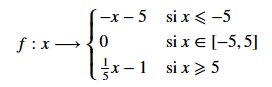
\includegraphics{medias/equation.png}

    \begin{Verbatim}[commandchars=\\\{\}]
{\color{incolor}In [{\color{incolor} }]:} \PY{c+c1}{\PYZsh{} donc par exemple}
        \PY{n}{exo\PYZus{}morceaux}\PY{o}{.}\PY{n}{example}\PY{p}{(}\PY{p}{)}
\end{Verbatim}


    \begin{Verbatim}[commandchars=\\\{\}]
{\color{incolor}In [{\color{incolor} }]:} \PY{c+c1}{\PYZsh{} à vous de jouer}
        
        \PY{k}{def} \PY{n+nf}{morceaux}\PY{p}{(}\PY{n}{x}\PY{p}{)}\PY{p}{:}
            \PY{k}{return} \PY{l+m+mi}{0} \PY{c+c1}{\PYZsh{} \PYZdq{}votre code\PYZdq{}}
\end{Verbatim}


    \begin{Verbatim}[commandchars=\\\{\}]
{\color{incolor}In [{\color{incolor} }]:} \PY{c+c1}{\PYZsh{} pour corriger votre code}
        \PY{n}{exo\PYZus{}morceaux}\PY{o}{.}\PY{n}{correction}\PY{p}{(}\PY{n}{morceaux}\PY{p}{)}
\end{Verbatim}


    \hypertarget{repruxe9sentation-graphique}{%
\subparagraph{Représentation
graphique}\label{repruxe9sentation-graphique}}

    L'exercice est maintenant terminé, mais nous allons voir ensemble
maintenant comment vous pourriez visualiser votre fonction.

Voici ce qui est attendu comme courbe pour \texttt{morceaux} (image
fixe)~:\\\\
 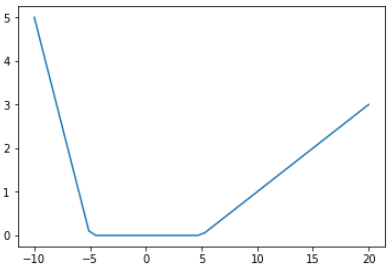
\includegraphics{medias/morceaux.png}

    En partant de votre code, vous pouvez produire votre propre courbe en
utilisant \texttt{numpy} et \texttt{matplotlib} comme ceci~:

    \begin{Verbatim}[commandchars=\\\{\}]
{\color{incolor}In [{\color{incolor} }]:} \PY{c+c1}{\PYZsh{} on importe les bibliothèques}
        \PY{k+kn}{import} \PY{n+nn}{numpy} \PY{k}{as} \PY{n+nn}{np}
        \PY{k+kn}{import} \PY{n+nn}{matplotlib}\PY{n+nn}{.}\PY{n+nn}{pyplot} \PY{k}{as} \PY{n+nn}{plt}
\end{Verbatim}


    \begin{Verbatim}[commandchars=\\\{\}]
{\color{incolor}In [{\color{incolor} }]:} \PY{c+c1}{\PYZsh{} un échantillon des X entre \PYZhy{}10 et 20}
        \PY{n}{X} \PY{o}{=} \PY{n}{np}\PY{o}{.}\PY{n}{linspace}\PY{p}{(}\PY{o}{\PYZhy{}}\PY{l+m+mi}{10}\PY{p}{,} \PY{l+m+mi}{20}\PY{p}{)}
        
        \PY{c+c1}{\PYZsh{} et les Y correspondants}
        \PY{n}{Y} \PY{o}{=} \PY{n}{np}\PY{o}{.}\PY{n}{vectorize}\PY{p}{(}\PY{n}{morceaux}\PY{p}{)}\PY{p}{(}\PY{n}{X}\PY{p}{)}
\end{Verbatim}


    \begin{Verbatim}[commandchars=\\\{\}]
{\color{incolor}In [{\color{incolor} }]:} \PY{c+c1}{\PYZsh{} on n\PYZsq{}a plus qu\PYZsq{}à dessiner}
        \PY{n}{plt}\PY{o}{.}\PY{n}{plot}\PY{p}{(}\PY{n}{X}\PY{p}{,} \PY{n}{Y}\PY{p}{)}
        \PY{n}{plt}\PY{o}{.}\PY{n}{show}\PY{p}{(}\PY{p}{)}
\end{Verbatim}
        \hypertarget{comptage-dans-les-chaines}{%
\section{Comptage dans les chaines}\label{comptage-dans-les-chaines}}

    \hypertarget{exercice---niveau-basique}{%
\subsection{Exercice - niveau basique}\label{exercice---niveau-basique}}

    Nous remercions Benoit Izac pour cette contribution aux exercices.

    \hypertarget{la-commande-unix-wc1}{%
\subsection{La commande UNIX wc(1)}\label{la-commande-unix-wc1}}

\begin{center}\rule{0.5\linewidth}{\linethickness}\end{center}

Sur les systèmes de type UNIX, la commande
\href{http://pubs.opengroup.org/onlinepubs/9699919799/utilities/wc.html}{wc}
permet de compter le nombre de lignes, de mots et d'octets (ou de
caractères) présents sur l'entrée standard ou contenus dans un fichier.\\

L'exercice consiste à écrire une fonction nommée \emph{wc} qui prendra
en argument une chaîne de caractères et retournera une liste contenant
trois éléments~:

\begin{enumerate}
\def\labelenumi{\arabic{enumi}.}
\tightlist
\item
  le nombre de lignes (plus précisément le nombre de retours à la
  ligne)~;
\item
  le nombre de mots (un mot étant séparé par des espaces)~;
\item
  le nombre de caractères (on utilisera uniquement le jeu de caractères
  ASCII).
\end{enumerate}

    \begin{Verbatim}[commandchars=\\\{\}]
{\color{incolor}In [{\color{incolor} }]:} \PY{c+c1}{\PYZsh{} chargement de l\PYZsq{}exercice}
        \PY{k+kn}{from} \PY{n+nn}{corrections}\PY{n+nn}{.}\PY{n+nn}{exo\PYZus{}wc} \PY{k}{import} \PY{n}{exo\PYZus{}wc}
\end{Verbatim}


    \begin{Verbatim}[commandchars=\\\{\}]
{\color{incolor}In [{\color{incolor} }]:} \PY{c+c1}{\PYZsh{} exemple}
        \PY{n}{exo\PYZus{}wc}\PY{o}{.}\PY{n}{example}\PY{p}{(}\PY{p}{)}
\end{Verbatim}


    \textbf{Indice}~: nous avons vu rapidement la boucle \texttt{for},
sachez toutefois qu'on peut tout à fait résoudre l'exercice en utilisant
uniquement la bibliothèque standard.\\

\textbf{Remarque}~: usuellement, ce genre de fonctions retournerait
plutôt un tuple qu'une liste, mais comme nous ne voyons les tuples que
la semaine prochaine..

    À vous de jouer~:

    \begin{Verbatim}[commandchars=\\\{\}]
{\color{incolor}In [{\color{incolor} }]:} \PY{c+c1}{\PYZsh{} la fonction à implémenter}
        \PY{k}{def} \PY{n+nf}{wc}\PY{p}{(}\PY{n}{string}\PY{p}{)}\PY{p}{:}
            \PY{c+c1}{\PYZsh{} remplacer pass par votre code}
            \PY{k}{pass}
\end{Verbatim}


    \begin{Verbatim}[commandchars=\\\{\}]
{\color{incolor}In [{\color{incolor} }]:} \PY{c+c1}{\PYZsh{} correction}
        \PY{n}{exo\PYZus{}wc}\PY{o}{.}\PY{n}{correction}\PY{p}{(}\PY{n}{wc}\PY{p}{)}
\end{Verbatim}
        \hypertarget{compruxe9hensions-1}{%
\section{Compréhensions (1)}\label{compruxe9hensions-1}}

    \hypertarget{exercice---niveau-basique}{%
\subsection{Exercice - niveau basique}\label{exercice---niveau-basique}}

    \hypertarget{liste-des-valeurs-dune-fonction}{%
\subsubsection{Liste des valeurs d'une
fonction}\label{liste-des-valeurs-dune-fonction}}

    \begin{Verbatim}[commandchars=\\\{\}]
{\color{incolor}In [{\color{incolor} }]:} \PY{c+c1}{\PYZsh{} Pour charger l\PYZsq{}exercice}
        \PY{k+kn}{from} \PY{n+nn}{corrections}\PY{n+nn}{.}\PY{n+nn}{exo\PYZus{}liste\PYZus{}p} \PY{k}{import} \PY{n}{exo\PYZus{}liste\PYZus{}P}
\end{Verbatim}


    On se donne une fonction polynomiale~:

\(P(x) = 2x^2 - 3x - 2\)

    On vous demande d'écrire une fonction \texttt{liste\_P} qui prend en
argument une liste de nombres réels \(x\) et qui retourne la liste des
valeurs \(P(x)\).

    \begin{Verbatim}[commandchars=\\\{\}]
{\color{incolor}In [{\color{incolor} }]:} \PY{c+c1}{\PYZsh{} voici un exemple de ce qui est attendu}
        \PY{n}{exo\PYZus{}liste\PYZus{}P}\PY{o}{.}\PY{n}{example}\PY{p}{(}\PY{p}{)}
\end{Verbatim}


    Écrivez votre code dans la cellule suivante (\emph{On vous suggère
d'écrire une fonction \texttt{P} qui implémente le polynôme mais ça
n'est pas strictement indispensable, seul le résultat de
\texttt{liste\_P} compte})~:

    \begin{Verbatim}[commandchars=\\\{\}]
{\color{incolor}In [{\color{incolor} }]:} \PY{k}{def} \PY{n+nf}{P}\PY{p}{(}\PY{n}{x}\PY{p}{)}\PY{p}{:}
            \PY{l+s+s2}{\PYZdq{}}\PY{l+s+s2}{\PYZlt{}votre code\PYZgt{}}\PY{l+s+s2}{\PYZdq{}}
        
        \PY{k}{def} \PY{n+nf}{liste\PYZus{}P}\PY{p}{(}\PY{n}{liste\PYZus{}x}\PY{p}{)}\PY{p}{:}
            \PY{l+s+s2}{\PYZdq{}}\PY{l+s+s2}{votre code}\PY{l+s+s2}{\PYZdq{}}
\end{Verbatim}


    Et vous pouvez le vérifier en évaluant cette cellule~:

    \begin{Verbatim}[commandchars=\\\{\}]
{\color{incolor}In [{\color{incolor} }]:} \PY{c+c1}{\PYZsh{} pour vérifier votre code}
        \PY{n}{exo\PYZus{}liste\PYZus{}P}\PY{o}{.}\PY{n}{correction}\PY{p}{(}\PY{n}{liste\PYZus{}P}\PY{p}{)}
\end{Verbatim}


    \begin{center}\rule{0.5\linewidth}{\linethickness}\end{center}

    \hypertarget{ruxe9cruxe9ation}{%
\subsection{Récréation}\label{ruxe9cruxe9ation}}

    Si vous avez correctement implémenté la fonction \texttt{liste\_P} telle
que demandé dans le premier exercice, vous pouvez visualiser le polynôme
\texttt{P} en utilisant \texttt{matplotlib} avec le code suivant~:

    \begin{Verbatim}[commandchars=\\\{\}]
{\color{incolor}In [{\color{incolor} }]:} \PY{c+c1}{\PYZsh{} on importe les bibliothèques}
        \PY{k+kn}{import} \PY{n+nn}{numpy} \PY{k}{as} \PY{n+nn}{np}
        \PY{k+kn}{import} \PY{n+nn}{matplotlib}\PY{n+nn}{.}\PY{n+nn}{pyplot} \PY{k}{as} \PY{n+nn}{plt}
\end{Verbatim}


    \begin{Verbatim}[commandchars=\\\{\}]
{\color{incolor}In [{\color{incolor} }]:} \PY{c+c1}{\PYZsh{} un échantillon des X entre \PYZhy{}10 et 10}
        \PY{n}{X} \PY{o}{=} \PY{n}{np}\PY{o}{.}\PY{n}{linspace}\PY{p}{(}\PY{o}{\PYZhy{}}\PY{l+m+mi}{10}\PY{p}{,} \PY{l+m+mi}{10}\PY{p}{)}
        
        \PY{c+c1}{\PYZsh{} et les Y correspondants}
        \PY{n}{Y} \PY{o}{=} \PY{n}{liste\PYZus{}P}\PY{p}{(}\PY{n}{X}\PY{p}{)}
\end{Verbatim}


    \begin{Verbatim}[commandchars=\\\{\}]
{\color{incolor}In [{\color{incolor} }]:} \PY{c+c1}{\PYZsh{} on n\PYZsq{}a plus qu\PYZsq{}à dessiner}
        \PY{n}{plt}\PY{o}{.}\PY{n}{plot}\PY{p}{(}\PY{n}{X}\PY{p}{,} \PY{n}{Y}\PY{p}{)}
        \PY{n}{plt}\PY{o}{.}\PY{n}{show}\PY{p}{(}\PY{p}{)}
\end{Verbatim}
        \hypertarget{compruxe9hensions-2}{%
\section{Compréhensions (2)}\label{compruxe9hensions-2}}

    \hypertarget{exercice---niveau-intermuxe9diaire}{%
\subsection{Exercice - niveau
intermédiaire}\label{exercice---niveau-intermuxe9diaire}}

    \hypertarget{mise-au-carruxe9}{%
\subsubsection{Mise au carré}\label{mise-au-carruxe9}}

    \begin{Verbatim}[commandchars=\\\{\}]
{\color{incolor}In [{\color{incolor} }]:} \PY{c+c1}{\PYZsh{} chargement de l\PYZsq{}exercice}
        \PY{k+kn}{from} \PY{n+nn}{corrections}\PY{n+nn}{.}\PY{n+nn}{exo\PYZus{}carre} \PY{k}{import} \PY{n}{exo\PYZus{}carre}
\end{Verbatim}


    On vous demande à présent d'écrire une fonction dans le même esprit que
ci-dessus. Cette fois, chaque ligne contient, séparés par des
points-virgules, une liste d'entiers, et on veut obtenir une nouvelle
chaîne avec les carrés de ces entiers, séparés par des deux-points.

À nouveau les lignes peuvent être remplies de manière approximative,
avec des espaces, des tabulations, ou même des points-virgules en trop,
que ce soit au début, à la fin, ou au milieu d'une ligne.

    \begin{Verbatim}[commandchars=\\\{\}]
{\color{incolor}In [{\color{incolor} }]:} \PY{c+c1}{\PYZsh{} exemples}
        \PY{n}{exo\PYZus{}carre}\PY{o}{.}\PY{n}{example}\PY{p}{(}\PY{p}{)}
\end{Verbatim}


    \begin{Verbatim}[commandchars=\\\{\}]
{\color{incolor}In [{\color{incolor} }]:} \PY{c+c1}{\PYZsh{} écrivez votre code ici}
        \PY{k}{def} \PY{n+nf}{carre}\PY{p}{(}\PY{n}{ligne}\PY{p}{)}\PY{p}{:}
            \PY{l+s+s2}{\PYZdq{}}\PY{l+s+s2}{\PYZlt{}votre\PYZus{}code\PYZgt{}}\PY{l+s+s2}{\PYZdq{}}
\end{Verbatim}


    \begin{Verbatim}[commandchars=\\\{\}]
{\color{incolor}In [{\color{incolor} }]:} \PY{c+c1}{\PYZsh{} pour corriger}
        \PY{n}{exo\PYZus{}carre}\PY{o}{.}\PY{n}{correction}\PY{p}{(}\PY{n}{carre}\PY{p}{)}
\end{Verbatim}
    
    \chapter{Renforcement des notions de base, références partagées}

        \hypertarget{les-fichiers}{%
\section{Les fichiers}\label{les-fichiers}}

    \hypertarget{compluxe9ment---niveau-basique}{%
\subsection{Complément - niveau
basique}\label{compluxe9ment---niveau-basique}}

    Voici quelques utilisations habituelles du type fichier en Python.

    \hypertarget{avec-un-context-manager}{%
\subsubsection{\texorpdfstring{Avec un \emph{context
manager}}{Avec un context manager}}\label{avec-un-context-manager}}

    Nous avons vu dans la vidéo les mécanismes de base sur les fichiers.
Nous avons vu notamment qu'il est important de bien fermer un fichier
après usage. On a vu aussi qu'il est recommandé de \textbf{toujours}
utiliser l'instruction \texttt{with} et de contrôler son encodage. Il
est donc recommandé de faire~:

    \begin{Verbatim}[commandchars=\\\{\}]
{\color{incolor}In [{\color{incolor}1}]:} \PY{c+c1}{\PYZsh{} avec un `with\PYZsq{} on garantit la fermeture du fichier}
        \PY{k}{with} \PY{n+nb}{open}\PY{p}{(}\PY{l+s+s2}{\PYZdq{}}\PY{l+s+s2}{foo.txt}\PY{l+s+s2}{\PYZdq{}}\PY{p}{,} \PY{l+s+s2}{\PYZdq{}}\PY{l+s+s2}{w}\PY{l+s+s2}{\PYZdq{}}\PY{p}{,} \PY{n}{encoding}\PY{o}{=}\PY{l+s+s1}{\PYZsq{}}\PY{l+s+s1}{utf\PYZhy{}8}\PY{l+s+s1}{\PYZsq{}}\PY{p}{)} \PY{k}{as} \PY{n}{sortie}\PY{p}{:}
            \PY{k}{for} \PY{n}{i} \PY{o+ow}{in} \PY{n+nb}{range}\PY{p}{(}\PY{l+m+mi}{2}\PY{p}{)}\PY{p}{:}
                \PY{n}{sortie}\PY{o}{.}\PY{n}{write}\PY{p}{(}\PY{n}{f}\PY{l+s+s2}{\PYZdq{}}\PY{l+s+si}{\PYZob{}i\PYZcb{}}\PY{l+s+se}{\PYZbs{}n}\PY{l+s+s2}{\PYZdq{}}\PY{p}{)}
\end{Verbatim}


    \hypertarget{les-modes-douverture}{%
\subsubsection{Les modes d'ouverture}\label{les-modes-douverture}}

    Les modes d'ouverture les plus utilisés sont~:
  
\begin{itemize}
	\item
	\texttt{\textquotesingle{}r\textquotesingle{}} (la chaîne contenant
	l'unique caractère \texttt{r}) pour ouvrir un fichier en lecture
	seulement~;
	\item
	\texttt{\textquotesingle{}w\textquotesingle{}} en écriture
	seulement~; le contenu précédent du fichier, s'il existait, est perdu~;
	\item
	\texttt{\textquotesingle{}a\textquotesingle{}} en écriture seulement~;
	mais pour ajouter du contenu en fin de fichier.
\end{itemize}

    Voici par exemple comment on pourrait ajouter deux lignes de texte dans
le fichier \texttt{foo.txt} qui contient, à ce stade du notebook, deux
entiers~:

    \begin{Verbatim}[commandchars=\\\{\}]
{\color{incolor}In [{\color{incolor}2}]:} \PY{c+c1}{\PYZsh{} on ouvre le fichier en mode \PYZsq{}a\PYZsq{} comme append (= ajouter)}
        \PY{k}{with} \PY{n+nb}{open}\PY{p}{(}\PY{l+s+s2}{\PYZdq{}}\PY{l+s+s2}{foo.txt}\PY{l+s+s2}{\PYZdq{}}\PY{p}{,} \PY{l+s+s2}{\PYZdq{}}\PY{l+s+s2}{a}\PY{l+s+s2}{\PYZdq{}}\PY{p}{,} \PY{n}{encoding}\PY{o}{=}\PY{l+s+s1}{\PYZsq{}}\PY{l+s+s1}{utf\PYZhy{}8}\PY{l+s+s1}{\PYZsq{}}\PY{p}{)} \PY{k}{as} \PY{n}{sortie}\PY{p}{:}
            \PY{k}{for} \PY{n}{i} \PY{o+ow}{in} \PY{n+nb}{range}\PY{p}{(}\PY{l+m+mi}{100}\PY{p}{,} \PY{l+m+mi}{102}\PY{p}{)}\PY{p}{:}
                \PY{n}{sortie}\PY{o}{.}\PY{n}{write}\PY{p}{(}\PY{n}{f}\PY{l+s+s2}{\PYZdq{}}\PY{l+s+si}{\PYZob{}i\PYZcb{}}\PY{l+s+se}{\PYZbs{}n}\PY{l+s+s2}{\PYZdq{}}\PY{p}{)}
\end{Verbatim}


    \begin{Verbatim}[commandchars=\\\{\}]
{\color{incolor}In [{\color{incolor}3}]:} \PY{c+c1}{\PYZsh{} maintenant on regarde ce que contient le fichier}
        \PY{k}{with} \PY{n+nb}{open}\PY{p}{(}\PY{l+s+s2}{\PYZdq{}}\PY{l+s+s2}{foo.txt}\PY{l+s+s2}{\PYZdq{}}\PY{p}{,} \PY{n}{encoding}\PY{o}{=}\PY{l+s+s1}{\PYZsq{}}\PY{l+s+s1}{utf\PYZhy{}8}\PY{l+s+s1}{\PYZsq{}}\PY{p}{)} \PY{k}{as} \PY{n}{entree}\PY{p}{:} \PY{c+c1}{\PYZsh{} remarquez que sans \PYZsq{}mode\PYZsq{}, on ouvre en lecture seule}
            \PY{k}{for} \PY{n}{line} \PY{o+ow}{in} \PY{n}{entree}\PY{p}{:}
                \PY{c+c1}{\PYZsh{} line contient déjà un retour à la ligne}
                \PY{n+nb}{print}\PY{p}{(}\PY{n}{line}\PY{p}{,} \PY{n}{end}\PY{o}{=}\PY{l+s+s1}{\PYZsq{}}\PY{l+s+s1}{\PYZsq{}}\PY{p}{)}
\end{Verbatim}


    \begin{Verbatim}[commandchars=\\\{\}]
0
1
100
101

    \end{Verbatim}

    Il existe de nombreuses variantes au mode d'ouverture, pour par
exemple~:
\begin{itemize}
	\item 
	ouvrir le fichier en lecture \emph{et} en écriture (mode
	\texttt{+})~;
	\item
	ouvrir le fichier en mode binaire (mode \texttt{b}).
\end{itemize}

Ces variantes sont décrites dans
\href{https://docs.python.org/3/library/functions.html\#open}{la section
sur la fonction built-in \texttt{open}} dans la documentation Python.

    \hypertarget{compluxe9ment---niveau-intermuxe9diaire}{%
\subsection{Complément - niveau
intermédiaire}\label{compluxe9ment---niveau-intermuxe9diaire}}

    \hypertarget{un-fichier-est-un-ituxe9rateur}{%
\subsubsection{Un fichier est un
itérateur}\label{un-fichier-est-un-ituxe9rateur}}

    Nous reparlerons des notions d'itérable et d'itérateur dans les semaines
suivantes. Pour l'instant, on peut dire qu'un fichier - qui donc
\textbf{est itérable} puisqu'on peut le lire par une boucle \texttt{for}
- est aussi \textbf{son propre itérateur}. Cela implique que l'on ne
peut le parcourir qu'une fois dans une boucle \texttt{for}. Pour le
reparcourir, il faut le fermer et l'ouvrir de nouveau.

    \begin{Verbatim}[commandchars=\\\{\}]
{\color{incolor}In [{\color{incolor}4}]:} \PY{c+c1}{\PYZsh{} un fichier est son propre itérateur}
\end{Verbatim}


    \begin{Verbatim}[commandchars=\\\{\}]
{\color{incolor}In [{\color{incolor}5}]:} \PY{k}{with} \PY{n+nb}{open}\PY{p}{(}\PY{l+s+s2}{\PYZdq{}}\PY{l+s+s2}{foo.txt}\PY{l+s+s2}{\PYZdq{}}\PY{p}{,} \PY{n}{encoding}\PY{o}{=}\PY{l+s+s1}{\PYZsq{}}\PY{l+s+s1}{utf\PYZhy{}8}\PY{l+s+s1}{\PYZsq{}}\PY{p}{)} \PY{k}{as} \PY{n}{entree}\PY{p}{:}
            \PY{n+nb}{print}\PY{p}{(}\PY{n}{entree}\PY{o}{.}\PY{n+nf+fm}{\PYZus{}\PYZus{}iter\PYZus{}\PYZus{}}\PY{p}{(}\PY{p}{)} \PY{o+ow}{is} \PY{n}{entree}\PY{p}{)}
\end{Verbatim}


    \begin{Verbatim}[commandchars=\\\{\}]
True

    \end{Verbatim}

    Par conséquent, écrire deux boucles \texttt{for} imbriquées sur
\textbf{le même objet fichier} ne \textbf{fonctionnerait pas} comme on
pourrait s'y attendre.

    \begin{Verbatim}[commandchars=\\\{\}]
{\color{incolor}In [{\color{incolor}6}]:} \PY{c+c1}{\PYZsh{} Si l\PYZsq{}on essaie d\PYZsq{}écrire deux boucles imbriquées}
        \PY{c+c1}{\PYZsh{} sur le même objet fichier, le résultat est inattendu}
        \PY{k}{with} \PY{n+nb}{open}\PY{p}{(}\PY{l+s+s2}{\PYZdq{}}\PY{l+s+s2}{foo.txt}\PY{l+s+s2}{\PYZdq{}}\PY{p}{,} \PY{n}{encoding}\PY{o}{=}\PY{l+s+s1}{\PYZsq{}}\PY{l+s+s1}{utf\PYZhy{}8}\PY{l+s+s1}{\PYZsq{}}\PY{p}{)} \PY{k}{as} \PY{n}{entree}\PY{p}{:}
            \PY{k}{for} \PY{n}{l1} \PY{o+ow}{in} \PY{n}{entree}\PY{p}{:}
                \PY{c+c1}{\PYZsh{} on enlève les fins de ligne}
                \PY{n}{l1} \PY{o}{=} \PY{n}{l1}\PY{o}{.}\PY{n}{strip}\PY{p}{(}\PY{p}{)}
                \PY{k}{for} \PY{n}{l2} \PY{o+ow}{in} \PY{n}{entree}\PY{p}{:}
                    \PY{c+c1}{\PYZsh{} on enlève les fins de ligne}
                    \PY{n}{l2} \PY{o}{=} \PY{n}{l2}\PY{o}{.}\PY{n}{strip}\PY{p}{(}\PY{p}{)}
                    \PY{n+nb}{print}\PY{p}{(}\PY{n}{l1}\PY{p}{,} \PY{l+s+s2}{\PYZdq{}}\PY{l+s+s2}{x}\PY{l+s+s2}{\PYZdq{}}\PY{p}{,} \PY{n}{l2}\PY{p}{)}
\end{Verbatim}


    \begin{Verbatim}[commandchars=\\\{\}]
0 x 1
0 x 100
0 x 101

    \end{Verbatim}

    \hypertarget{compluxe9ment---niveau-avancuxe9}{%
\subsection{Complément - niveau
avancé}\label{compluxe9ment---niveau-avancuxe9}}

    \hypertarget{autres-muxe9thodes}{%
\subsubsection{Autres méthodes}\label{autres-muxe9thodes}}

    Vous pouvez également accéder à des fonctions de beaucoup plus bas
niveau, notamment celle fournies directement par le système
d'exploitation~; nous allons en décrire deux parmi les plus utiles.

    \hypertarget{digression---repr}{%
\subparagraph{\texorpdfstring{Digression -
\texttt{repr()}}{Digression - repr()}\\\\}\label{digression---repr}}

    Comme nous allons utiliser maintenant des outils d'assez bas niveau pour
lire du texte, pour examiner ce texte nous allons utiliser la fonction
\texttt{repr()}, et voici pourquoi~:

    \begin{Verbatim}[commandchars=\\\{\}]
{\color{incolor}In [{\color{incolor}7}]:} \PY{c+c1}{\PYZsh{} construisons à la main une chaîne qui contient deux lignes}
        \PY{n}{lines} \PY{o}{=} \PY{l+s+s2}{\PYZdq{}}\PY{l+s+s2}{abc}\PY{l+s+s2}{\PYZdq{}} \PY{o}{+} \PY{l+s+s2}{\PYZdq{}}\PY{l+s+se}{\PYZbs{}n}\PY{l+s+s2}{\PYZdq{}} \PY{o}{+} \PY{l+s+s2}{\PYZdq{}}\PY{l+s+s2}{def}\PY{l+s+s2}{\PYZdq{}}  \PY{o}{+} \PY{l+s+s2}{\PYZdq{}}\PY{l+s+se}{\PYZbs{}n}\PY{l+s+s2}{\PYZdq{}}
\end{Verbatim}


    \begin{Verbatim}[commandchars=\\\{\}]
{\color{incolor}In [{\color{incolor}8}]:} \PY{c+c1}{\PYZsh{} si on l\PYZsq{}imprime on voit bien les retours à la ligne}
        \PY{c+c1}{\PYZsh{} d\PYZsq{}ailleurs on sait qu\PYZsq{}il n\PYZsq{}est pas utile}
        \PY{c+c1}{\PYZsh{} d\PYZsq{}ajouter un retour à la ligne à la fin}
        \PY{n+nb}{print}\PY{p}{(}\PY{n}{lines}\PY{p}{,} \PY{n}{end}\PY{o}{=}\PY{l+s+s2}{\PYZdq{}}\PY{l+s+s2}{\PYZdq{}}\PY{p}{)}
\end{Verbatim}


    \begin{Verbatim}[commandchars=\\\{\}]
abc
def

    \end{Verbatim}

    \begin{Verbatim}[commandchars=\\\{\}]
{\color{incolor}In [{\color{incolor}9}]:} \PY{c+c1}{\PYZsh{} vérifions que repr() nous permet de bien}
        \PY{c+c1}{\PYZsh{} voir le contenu de cette chaine}
        \PY{n+nb}{print}\PY{p}{(}\PY{n+nb}{repr}\PY{p}{(}\PY{n}{lines}\PY{p}{)}\PY{p}{)}
\end{Verbatim}


    \begin{Verbatim}[commandchars=\\\{\}]
'abc\textbackslash{}ndef\textbackslash{}n'

    \end{Verbatim}

    \hypertarget{lire-un-contenu---bas-niveau}{%
\subparagraph{Lire un contenu - bas
niveau\\\\}\label{lire-un-contenu---bas-niveau}}

    Revenons aux fichiers~; la méthode \texttt{read()} permet de lire dans
le fichier un buffer d'une certaine taille~:

    \begin{Verbatim}[commandchars=\\\{\}]
{\color{incolor}In [{\color{incolor}10}]:} \PY{c+c1}{\PYZsh{} read() retourne TOUT le contenu}
         \PY{c+c1}{\PYZsh{} ne pas utiliser avec de très gros fichiers bien sûr}
         
         \PY{c+c1}{\PYZsh{} une autre façon de montrer tout le contenu du fichier}
         \PY{k}{with} \PY{n+nb}{open}\PY{p}{(}\PY{l+s+s2}{\PYZdq{}}\PY{l+s+s2}{foo.txt}\PY{l+s+s2}{\PYZdq{}}\PY{p}{,} \PY{n}{encoding}\PY{o}{=}\PY{l+s+s1}{\PYZsq{}}\PY{l+s+s1}{utf\PYZhy{}8}\PY{l+s+s1}{\PYZsq{}}\PY{p}{)} \PY{k}{as} \PY{n}{entree}\PY{p}{:}
             \PY{n}{full\PYZus{}contents} \PY{o}{=} \PY{n}{entree}\PY{o}{.}\PY{n}{read}\PY{p}{(}\PY{p}{)}
             \PY{n+nb}{print}\PY{p}{(}\PY{n}{f}\PY{l+s+s2}{\PYZdq{}}\PY{l+s+s2}{Contenu complet}\PY{l+s+se}{\PYZbs{}n}\PY{l+s+si}{\PYZob{}full\PYZus{}contents\PYZcb{}}\PY{l+s+s2}{\PYZdq{}}\PY{p}{,} \PY{n}{end}\PY{o}{=}\PY{l+s+s2}{\PYZdq{}}\PY{l+s+s2}{\PYZdq{}}\PY{p}{)}
\end{Verbatim}


    \begin{Verbatim}[commandchars=\\\{\}]
Contenu complet
0
1
100
101

    \end{Verbatim}

    \begin{Verbatim}[commandchars=\\\{\}]
{\color{incolor}In [{\color{incolor}11}]:} \PY{c+c1}{\PYZsh{} lire dans le fichier deux blocs de quatre caractères}
         \PY{k}{with} \PY{n+nb}{open}\PY{p}{(}\PY{l+s+s2}{\PYZdq{}}\PY{l+s+s2}{foo.txt}\PY{l+s+s2}{\PYZdq{}}\PY{p}{,} \PY{n}{encoding}\PY{o}{=}\PY{l+s+s1}{\PYZsq{}}\PY{l+s+s1}{utf\PYZhy{}8}\PY{l+s+s1}{\PYZsq{}}\PY{p}{)} \PY{k}{as} \PY{n}{entree}\PY{p}{:}
             \PY{k}{for} \PY{n}{bloc} \PY{o+ow}{in} \PY{n+nb}{range}\PY{p}{(}\PY{l+m+mi}{2}\PY{p}{)}\PY{p}{:}
                 \PY{n+nb}{print}\PY{p}{(}\PY{n}{f}\PY{l+s+s2}{\PYZdq{}}\PY{l+s+s2}{Bloc }\PY{l+s+si}{\PYZob{}bloc\PYZcb{}}\PY{l+s+s2}{ \PYZgt{}\PYZgt{}}\PY{l+s+s2}{\PYZob{}}\PY{l+s+s2}{repr(entree.read(4))\PYZcb{}\PYZlt{}\PYZlt{}}\PY{l+s+s2}{\PYZdq{}}\PY{p}{)}
\end{Verbatim}


    \begin{Verbatim}[commandchars=\\\{\}]
Bloc 0 >>'0\textbackslash{}n1\textbackslash{}n'<<
Bloc 1 >>'100\textbackslash{}n'<<

    \end{Verbatim}

    On voit donc que chaque bloc contient bien quatre caractères en comptant
les sauts de ligne~:

\begin{longtable}[]{@{}lr@{}}
\toprule
bloc \# & contenu\tabularnewline
\midrule
\endhead
0 & un \texttt{0}, un \emph{newline}, un \texttt{1}, un
\emph{newline}\tabularnewline
1 & un \texttt{1}, deux \texttt{0}, un \emph{newline}\tabularnewline
\bottomrule
\end{longtable}

    \hypertarget{la-muxe9thode-flush}{%
\subparagraph{\texorpdfstring{La méthode
\texttt{flush}}{La méthode flush}\\\\}\label{la-muxe9thode-flush}}

    Les entrées-sorties sur fichier sont bien souvent \emph{bufferisées} par
le système d'exploitation. Cela signifie qu'un appel à \texttt{write} ne
provoque pas forcément une écriture immédiate, car pour des raisons de
performance on attend d'avoir suffisamment de matière avant d'écrire sur
le disque.\\

Il y a des cas où ce comportement peut s'avérer gênant, et où on a
besoin d'écrire immédiatement (et donc de vider le \emph{buffer}), et
c'est le propos de la méthode \texttt{flush}.

    \hypertarget{fichiers-textuels-et-fichiers-binaires}{%
\subsubsection{Fichiers textuels et fichiers
binaires}\label{fichiers-textuels-et-fichiers-binaires}}

    De la même façon que le langage propose les deux types \texttt{str} et
\texttt{bytes}, il est possible d'ouvrir un fichier en mode
\emph{textuel} ou en mode \emph{binaire}.\\

    Les fichiers que nous avons vus jusqu'ici étaient ouverts en mode
\emph{textuel} (c'est le défaut), et c'est pourquoi nous avons interagi
avec eux avec des objets de type \texttt{str}~:

    \begin{Verbatim}[commandchars=\\\{\}]
{\color{incolor}In [{\color{incolor}12}]:} \PY{c+c1}{\PYZsh{} un fichier ouvert en mode textuel nous donne des str}
         \PY{k}{with} \PY{n+nb}{open}\PY{p}{(}\PY{l+s+s1}{\PYZsq{}}\PY{l+s+s1}{foo.txt}\PY{l+s+s1}{\PYZsq{}}\PY{p}{,} \PY{n}{encoding}\PY{o}{=}\PY{l+s+s1}{\PYZsq{}}\PY{l+s+s1}{utf\PYZhy{}8}\PY{l+s+s1}{\PYZsq{}}\PY{p}{)} \PY{k}{as} \PY{n+nb}{input}\PY{p}{:}
             \PY{k}{for} \PY{n}{line} \PY{o+ow}{in} \PY{n+nb}{input}\PY{p}{:}
                 \PY{n+nb}{print}\PY{p}{(}\PY{l+s+s2}{\PYZdq{}}\PY{l+s+s2}{on a lu un objet de type}\PY{l+s+s2}{\PYZdq{}}\PY{p}{,} \PY{n+nb}{type}\PY{p}{(}\PY{n}{line}\PY{p}{)}\PY{p}{)}
\end{Verbatim}


    \begin{Verbatim}[commandchars=\\\{\}]
on a lu un objet de type <class 'str'>
on a lu un objet de type <class 'str'>
on a lu un objet de type <class 'str'>
on a lu un objet de type <class 'str'>

    \end{Verbatim}

    Lorsque ce n'est pas le comportement souhaité, on peut~:
    
\begin{itemize}
	\item 
	ouvrir le fichier en mode \emph{binaire} - pour cela on ajoute le caractère
	\texttt{b} au mode d'ouverture~;
	\item
	et on peut alors interagir avec le fichier avec des objets de type \texttt{bytes}
\end{itemize}

    Pour illustrer ce trait, nous allons~: 0. créer un fichier en mode
texte, et y insérer du texte en UTF-8~; 0. relire le fichier en mode
binaire, et retrouver le codage des différents caractères.

    \begin{Verbatim}[commandchars=\\\{\}]
{\color{incolor}In [{\color{incolor}13}]:} \PY{c+c1}{\PYZsh{} phase 1 : on écrit un fichier avec du texte en UTF\PYZhy{}8}
         \PY{c+c1}{\PYZsh{} on ouvre donc le fichier en mode texte}
         \PY{c+c1}{\PYZsh{} en toute rigueur il faut préciser l\PYZsq{}encodage,}
         \PY{c+c1}{\PYZsh{} si on ne le fait pas il sera déterminé}
         \PY{c+c1}{\PYZsh{} à partir de vos réglages système}
         \PY{k}{with} \PY{n+nb}{open}\PY{p}{(}\PY{l+s+s1}{\PYZsq{}}\PY{l+s+s1}{strbytes}\PY{l+s+s1}{\PYZsq{}}\PY{p}{,} \PY{l+s+s1}{\PYZsq{}}\PY{l+s+s1}{w}\PY{l+s+s1}{\PYZsq{}}\PY{p}{,} \PY{n}{encoding}\PY{o}{=}\PY{l+s+s1}{\PYZsq{}}\PY{l+s+s1}{utf\PYZhy{}8}\PY{l+s+s1}{\PYZsq{}}\PY{p}{)} \PY{k}{as} \PY{n}{output}\PY{p}{:}
             \PY{n}{output}\PY{o}{.}\PY{n}{write}\PY{p}{(}\PY{l+s+s2}{\PYZdq{}}\PY{l+s+s2}{déjà l}\PY{l+s+s2}{\PYZsq{}}\PY{l+s+s2}{été}\PY{l+s+se}{\PYZbs{}n}\PY{l+s+s2}{\PYZdq{}}\PY{p}{)}
\end{Verbatim}


    \begin{Verbatim}[commandchars=\\\{\}]
{\color{incolor}In [{\color{incolor}14}]:} \PY{c+c1}{\PYZsh{} phase 2: on ouvre le fichier en mode binaire}
         \PY{k}{with} \PY{n+nb}{open}\PY{p}{(}\PY{l+s+s1}{\PYZsq{}}\PY{l+s+s1}{strbytes}\PY{l+s+s1}{\PYZsq{}}\PY{p}{,} \PY{l+s+s1}{\PYZsq{}}\PY{l+s+s1}{rb}\PY{l+s+s1}{\PYZsq{}}\PY{p}{)} \PY{k}{as} \PY{n}{rawinput}\PY{p}{:}
             \PY{c+c1}{\PYZsh{} on lit tout le contenu}
             \PY{n}{octets} \PY{o}{=} \PY{n}{rawinput}\PY{o}{.}\PY{n}{read}\PY{p}{(}\PY{p}{)}
             \PY{c+c1}{\PYZsh{} qui est de type bytes}
             \PY{n+nb}{print}\PY{p}{(}\PY{l+s+s2}{\PYZdq{}}\PY{l+s+s2}{on a lu un objet de type}\PY{l+s+s2}{\PYZdq{}}\PY{p}{,} \PY{n+nb}{type}\PY{p}{(}\PY{n}{octets}\PY{p}{)}\PY{p}{)}
             \PY{c+c1}{\PYZsh{} si on regarde chaque octet un par un}
             \PY{k}{for} \PY{n}{i}\PY{p}{,} \PY{n}{octet} \PY{o+ow}{in} \PY{n+nb}{enumerate}\PY{p}{(}\PY{n}{octets}\PY{p}{)}\PY{p}{:}
                 \PY{n+nb}{print}\PY{p}{(}\PY{n}{f}\PY{l+s+s2}{\PYZdq{}}\PY{l+s+si}{\PYZob{}i\PYZcb{}}\PY{l+s+s2}{ → }\PY{l+s+s2}{\PYZob{}}\PY{l+s+s2}{repr(chr(octet))\PYZcb{} [}\PY{l+s+s2}{\PYZob{}}\PY{l+s+s2}{hex(octet)\PYZcb{}]}\PY{l+s+s2}{\PYZdq{}}\PY{p}{)}
\end{Verbatim}


    \begin{Verbatim}[commandchars=\\\{\}]
on a lu un objet de type <class 'bytes'>
0 → 'd' [0x64]
1 → 'Ã' [0xc3]
2 → '©' [0xa9]
3 → 'j' [0x6a]
4 → 'Ã' [0xc3]
5 → '\textbackslash{}xa0' [0xa0]
6 → ' ' [0x20]
7 → 'l' [0x6c]
8 → "'" [0x27]
9 → 'Ã' [0xc3]
10 → '©' [0xa9]
11 → 't' [0x74]
12 → 'Ã' [0xc3]
13 → '©' [0xa9]
14 → '\textbackslash{}r' [0xd]
15 → '\textbackslash{}n' [0xa]

    \end{Verbatim}

    Vous retrouvez ainsi le fait que l'unique caractère Unicode \texttt{é} a
été encodé par UTF-8 sous la forme de deux octets de code hexadécimal
\texttt{0xc3} et \texttt{0xa9}.\\

    Vous pouvez également consulter ce site qui visualise l'encodage UTF-8,
avec notre séquence d'entrée~:\\

\href{https://mothereff.in/utf-8\#d\%C3\%A9j\%C3\%A0\%20l\%27\%C3\%A9t\%C3\%A9\%0A}{https://mothereff.in/utf-8\#d\%C3\%A9j\%C3\%A0\%20l\%27\%C3\%A9t\%C3\%A9\%0A}

    \begin{Verbatim}[commandchars=\\\{\}]
{\color{incolor}In [{\color{incolor}15}]:} \PY{c+c1}{\PYZsh{} on peut comparer le nombre d\PYZsq{}octets et le nombre de caractères}
         \PY{k}{with} \PY{n+nb}{open}\PY{p}{(}\PY{l+s+s1}{\PYZsq{}}\PY{l+s+s1}{strbytes}\PY{l+s+s1}{\PYZsq{}}\PY{p}{,} \PY{n}{encoding}\PY{o}{=}\PY{l+s+s1}{\PYZsq{}}\PY{l+s+s1}{utf\PYZhy{}8}\PY{l+s+s1}{\PYZsq{}}\PY{p}{)} \PY{k}{as} \PY{n}{textfile}\PY{p}{:}
             \PY{n+nb}{print}\PY{p}{(}\PY{n}{f}\PY{l+s+s2}{\PYZdq{}}\PY{l+s+s2}{en mode texte, }\PY{l+s+s2}{\PYZob{}}\PY{l+s+s2}{len(textfile.read())\PYZcb{} caractères}\PY{l+s+s2}{\PYZdq{}}\PY{p}{)}
         \PY{k}{with} \PY{n+nb}{open}\PY{p}{(}\PY{l+s+s1}{\PYZsq{}}\PY{l+s+s1}{strbytes}\PY{l+s+s1}{\PYZsq{}}\PY{p}{,} \PY{l+s+s1}{\PYZsq{}}\PY{l+s+s1}{rb}\PY{l+s+s1}{\PYZsq{}}\PY{p}{)} \PY{k}{as} \PY{n}{binfile}\PY{p}{:}
             \PY{n+nb}{print}\PY{p}{(}\PY{n}{f}\PY{l+s+s2}{\PYZdq{}}\PY{l+s+s2}{en mode binaire, }\PY{l+s+s2}{\PYZob{}}\PY{l+s+s2}{len(binfile.read())\PYZcb{} octets}\PY{l+s+s2}{\PYZdq{}}\PY{p}{)}
\end{Verbatim}


    \begin{Verbatim}[commandchars=\\\{\}]
en mode texte, 11 caractères
en mode binaire, 16 octets

    \end{Verbatim}

    Ce qui correspond au fait que nos quatre caractères non-ASCII (3 x
\texttt{é} et 1 x \texttt{à}) sont tous encodés par UTF-8 comme deux
octets, comme vous pouvez vous en assurer
\href{https://mothereff.in/utf-8\#\%C3\%A9}{ici pour \texttt{é}} et
\href{https://mothereff.in/utf-8\#\%C3\%A0}{là pour \texttt{à}}.

    \hypertarget{pour-en-savoir-plus}{%
\subsubsection{Pour en savoir plus}\label{pour-en-savoir-plus}}

    Pour une description exhaustive vous pouvez vous reporter~:
    
\begin{itemize}
	\item 
	au \href{https://docs.python.org/3/glossary.html\#term-file-object}{glossaire
	sur la notion de \texttt{object\ file}},
	\item
	et aussi et surtout \href{https://docs.python.org/3/library/io.html\#module-io}{au module
	\texttt{io}} qui décrit plus en détail les fonctionnalités disponibles.
\end{itemize}    
        \hypertarget{fichiers-et-utilitaires}{%
\section{Fichiers et utilitaires}\label{fichiers-et-utilitaires}}

    \hypertarget{compluxe9ment---niveau-basique}{%
\subsection{Complément - niveau
basique}\label{compluxe9ment---niveau-basique}}

    Outre les objets fichiers créés avec la fonction \texttt{open}, comme on
l'a vu dans la vidéo, et qui servent à lire et écrire à un endroit
précis, une application a besoin d'un minimum d'utilitaires pour
\textbf{parcourir l'arborescence de répertoires et fichiers}, c'est
notre propos dans ce complément.

    \hypertarget{le-module-os.path-obsoluxe8te}{%
\subsubsection{\texorpdfstring{Le module \texttt{os.path}
(obsolète)}{Le module os.path (obsolète)}}\label{le-module-os.path-obsoluxe8te}}

    Avant la version python-3.4, la librairie standard offrait une
conjonction d'outils pour ce type de fonctionnalités:

\begin{itemize}
\tightlist
\item
  le module \texttt{os.path}, pour faire des calculs sur les les chemins
  et noms de fichiers
  \href{https://docs.python.org/3/library/os.html}{doc},
\item
  le module \texttt{os} pour certaines fonctions complémentaires comme
  renommer ou détruire un fichier
  \href{https://docs.python.org/3/library/os.path.html}{doc},
\item
  et enfin le module \texttt{glob} pour la recherche de fichiers, par
  exemple pour trouver tous les fichiers en \texttt{*.txt}
  \href{https://docs.python.org/3/library/glob.html}{doc}.
\end{itemize}

    Cet ensemble un peu disparate a été remplacé par une \textbf{librairie
unique \texttt{pathlib}}, qui fournit toutes ces fonctionnalités sous un
interface unique et moderne, que nous \textbf{recommandons} évidemment
d'utiliser pour \textbf{du nouveau code}.\\

Avant d'aborder \texttt{pathlib}, voici un très bref aperçu de ces trois
anciens modules, pour le cas - assez probable - où vous les
rencontreriez dans du code existant; tous les noms qui suivent
correspondent à des \textbf{fonctions} - par opposition à
\texttt{pathlib} qui, comme nous allons le voir, offre une interface
orientée objet:

    \begin{itemize}
\tightlist
\item
  \texttt{os.path.join} ajoute `/' ou '' entre deux morceaux de chemin,
  selon l'OS
\item
  \texttt{os.path.basename} trouve le nom de fichier dans un chemin
\item
  \texttt{os.path.dirname} trouve le nom du directory dans un chemin
\item
  \texttt{os.path.abspath} calcule un chemin absolu, c'est-à-dire à
  partir de la racine du filesystem
\end{itemize}

    \begin{itemize}
\tightlist
\item
  \texttt{os.path.exists} pour savoir si un chemin existe ou pas
  (fichier ou répertoire)
\item
  \texttt{os.path.isfile} (et \texttt{isdir}) pour savoir si un chemin
  est un fichier (et un répertoire)
\item
  \texttt{os.path.getsize} pour obtenir la taille du fichier
\item
  \texttt{os.path.getatime} et aussi \texttt{getmtime} et
  \texttt{getctime} pour obtenir les dates de création/modification d'un
  fichier
\end{itemize}

    \begin{itemize}
\tightlist
\item
  \texttt{os.remove} (ou son ancien nom \texttt{os.unlink}), qui permet
  de supprimer un fichier
\item
  \texttt{os.rmdir} pour supprimer un répertoire (mais qui doit être
  vide)
\item
  \texttt{os.removedirs} pour supprimer tout un répertoire avec son
  contenu, récursivement si nécessaire
\item
  \texttt{os.rename} pour renommer un fichier
\end{itemize}

    \begin{itemize}
\tightlist
\item
  \texttt{glob.glob} comme dans par exemple \texttt{glob.glob("*.txt")}
\end{itemize}

    \hypertarget{le-module-pathlib}{%
\subsubsection{\texorpdfstring{Le module
\texttt{pathlib}}{Le module pathlib}}\label{le-module-pathlib}}

    C'est la méthode recommandée aujourd'hui pour travailler sur les
fichiers et répertoires.

    \hypertarget{orientuxe9-objet}{%
\subparagraph{Orienté Objet\\\\}\label{orientuxe9-objet}}

    Comme on l'a mentionné \texttt{pathlib} offre une interface orientée
objet; mais qu'est-ce que ça veut dire au juste ?\\

Ceci nous donne un prétexte pour une première application pratique des
notions de module (que nous avons introduits en fin de semaine 2) et de
classe (que nous allons voir en fin de semaine).\\

    De même que le langage nous propose les types \emph{builtin}
\texttt{int} et \texttt{str}, le module \texttt{pathlib} nous expose
\textbf{un type} (on dira plutôt \textbf{une classe}) qui s'appelle
\texttt{Path}, que nous allons importer comme ceci:

    \begin{Verbatim}[commandchars=\\\{\}]
{\color{incolor}In [{\color{incolor}1}]:} \PY{k+kn}{from} \PY{n+nn}{pathlib} \PY{k}{import} \PY{n}{Path}
\end{Verbatim}


    Nous allons faire tourner un petit scénario qui va créer un fichier:

    \begin{Verbatim}[commandchars=\\\{\}]
{\color{incolor}In [{\color{incolor}2}]:} \PY{c+c1}{\PYZsh{} le nom de notre fichier jouet }
        \PY{n}{nom} \PY{o}{=} \PY{l+s+s1}{\PYZsq{}}\PY{l+s+s1}{fichier\PYZhy{}temoin}\PY{l+s+s1}{\PYZsq{}}
\end{Verbatim}


    Pour commencer, nous allons vérifier si le fichier en question existe.

Pour ça nous créons un \textbf{objet} qui est une \textbf{instance} de
la classe \texttt{Path}, comme ceci:

    \begin{Verbatim}[commandchars=\\\{\}]
{\color{incolor}In [{\color{incolor}3}]:} \PY{c+c1}{\PYZsh{} on crée un objet de la classe Path, associé au nom de fichier}
        \PY{n}{path} \PY{o}{=} \PY{n}{Path}\PY{p}{(}\PY{n}{nom}\PY{p}{)}
\end{Verbatim}


    Vous remarquez que c'est consistent avec par exemple:

    \begin{Verbatim}[commandchars=\\\{\}]
{\color{incolor}In [{\color{incolor}4}]:} \PY{c+c1}{\PYZsh{} transformer un float en int}
        \PY{n}{i} \PY{o}{=} \PY{n+nb}{int}\PY{p}{(}\PY{l+m+mf}{3.5}\PY{p}{)}
\end{Verbatim}


    en ce sens que le type (\texttt{int} ou \texttt{Path}) se comporte comme
une usine pour créer des objets du type en question.\\

    Quoi qu'il en soit, cet objet \texttt{path} offre un certain nombre de
méthodes; pour les voir puisque nous sommes dans un notebook, je vous
invite dans la cellule suivante à utiliser l'aide en ligne en appuyant
sur la touche `Tabulation' après avoir ajouté un \texttt{.} comme si
vous alliez envoyer une méthode à cet objet

\begin{verbatim}
path.[taper la touche TAB]
\end{verbatim}

et le notebook vous montrera la liste des méthodes disponibles.

    \begin{Verbatim}[commandchars=\\\{\}]
{\color{incolor}In [{\color{incolor}5}]:} \PY{c+c1}{\PYZsh{} ajouter un . et utilisez la touche \PYZlt{}Tabulation\PYZgt{}}
        \PY{n}{path}\PY{o}{.}\PY{n}{chmod}
\end{Verbatim}


\begin{Verbatim}[commandchars=\\\{\}]
{\color{outcolor}Out[{\color{outcolor}5}]:} <bound method Path.chmod of WindowsPath('fichier-temoin')>
\end{Verbatim}
            
    Ainsi par exemple on peut savoir si le fichier existe avec la méthode
\texttt{exists()}

    \begin{Verbatim}[commandchars=\\\{\}]
{\color{incolor}In [{\color{incolor}6}]:} \PY{c+c1}{\PYZsh{} au départ le fichier n\PYZsq{}existe pas}
        \PY{n}{path}\PY{o}{.}\PY{n}{exists}\PY{p}{(}\PY{p}{)}
\end{Verbatim}


\begin{Verbatim}[commandchars=\\\{\}]
{\color{outcolor}Out[{\color{outcolor}6}]:} False
\end{Verbatim}
            
    \begin{Verbatim}[commandchars=\\\{\}]
{\color{incolor}In [{\color{incolor}7}]:} \PY{c+c1}{\PYZsh{} si j\PYZsq{}écris dedans je le crée}
        \PY{k}{with} \PY{n+nb}{open}\PY{p}{(}\PY{n}{nom}\PY{p}{,} \PY{l+s+s1}{\PYZsq{}}\PY{l+s+s1}{w}\PY{l+s+s1}{\PYZsq{}}\PY{p}{,} \PY{n}{encoding}\PY{o}{=}\PY{l+s+s1}{\PYZsq{}}\PY{l+s+s1}{utf\PYZhy{}8}\PY{l+s+s1}{\PYZsq{}}\PY{p}{)} \PY{k}{as} \PY{n}{output}\PY{p}{:}
            \PY{n}{output}\PY{o}{.}\PY{n}{write}\PY{p}{(}\PY{l+s+s1}{\PYZsq{}}\PY{l+s+s1}{0123456789}\PY{l+s+se}{\PYZbs{}n}\PY{l+s+s1}{\PYZsq{}}\PY{p}{)}
\end{Verbatim}


    \begin{Verbatim}[commandchars=\\\{\}]
{\color{incolor}In [{\color{incolor}8}]:} \PY{c+c1}{\PYZsh{} et maintenant il existe}
        \PY{n}{path}\PY{o}{.}\PY{n}{exists}\PY{p}{(}\PY{p}{)}
\end{Verbatim}


\begin{Verbatim}[commandchars=\\\{\}]
{\color{outcolor}Out[{\color{outcolor}8}]:} True
\end{Verbatim}
            
    \hypertarget{muxe9tadonnuxe9es}{%
\subparagraph{Métadonnées\\\\}\label{muxe9tadonnuxe9es}}

    Voici quelques exemples qui montrent comment accéder aux métadonnées de
ce fichier:

    \begin{Verbatim}[commandchars=\\\{\}]
{\color{incolor}In [{\color{incolor}9}]:} \PY{c+c1}{\PYZsh{} cette méthode retourne (en un seul appel système) les métadonnées agrégées}
        \PY{n}{path}\PY{o}{.}\PY{n}{stat}\PY{p}{(}\PY{p}{)}
\end{Verbatim}


\begin{Verbatim}[commandchars=\\\{\}]
{\color{outcolor}Out[{\color{outcolor}9}]:} os.stat\_result(st\_mode=33206, st\_ino=2251799814156457, st\_dev=571766744, st\_nlink=1, st\_uid=0, st\_gid=0, st\_size=12, st\_atime=1537703765, st\_mtime=1537703765, st\_ctime=1537703765)
\end{Verbatim}
            
    Pour ceux que ça intéresse, l'objet retourné par cette méthode
\texttt{stat} est un \texttt{namedtuple}, que l'on va voir très bientôt.\\

On accède aux différentes informations comme ceci:

    \begin{Verbatim}[commandchars=\\\{\}]
{\color{incolor}In [{\color{incolor}10}]:} \PY{c+c1}{\PYZsh{} la taille du fichier en octets est de 11 }
         \PY{c+c1}{\PYZsh{} car il faut compter un caractère \PYZdq{}newline\PYZdq{} en fin de ligne }
         \PY{n}{path}\PY{o}{.}\PY{n}{stat}\PY{p}{(}\PY{p}{)}\PY{o}{.}\PY{n}{st\PYZus{}size}
\end{Verbatim}


\begin{Verbatim}[commandchars=\\\{\}]
{\color{outcolor}Out[{\color{outcolor}10}]:} 12
\end{Verbatim}
            
    \begin{Verbatim}[commandchars=\\\{\}]
{\color{incolor}In [{\color{incolor}11}]:} \PY{c+c1}{\PYZsh{} la date de dernière modification, sous forme d\PYZsq{}un entier}
         \PY{c+c1}{\PYZsh{} c\PYZsq{}est le nombre de secondes depuis le 1er Janvier 1970}
         \PY{n}{mtime} \PY{o}{=} \PY{n}{path}\PY{o}{.}\PY{n}{stat}\PY{p}{(}\PY{p}{)}\PY{o}{.}\PY{n}{st\PYZus{}mtime}
         \PY{n}{mtime}
\end{Verbatim}


\begin{Verbatim}[commandchars=\\\{\}]
{\color{outcolor}Out[{\color{outcolor}11}]:} 1537703765.728249
\end{Verbatim}
            
    \begin{Verbatim}[commandchars=\\\{\}]
{\color{incolor}In [{\color{incolor}12}]:} \PY{c+c1}{\PYZsh{} que je peux rendre lisible comme ceci}
         \PY{c+c1}{\PYZsh{} en anticipant sur le module datetime}
         \PY{k+kn}{from} \PY{n+nn}{datetime} \PY{k}{import} \PY{n}{datetime}
         \PY{n}{mtime\PYZus{}datetime} \PY{o}{=} \PY{n}{datetime}\PY{o}{.}\PY{n}{fromtimestamp}\PY{p}{(}\PY{n}{mtime}\PY{p}{)}
         \PY{n}{mtime\PYZus{}datetime}
\end{Verbatim}


\begin{Verbatim}[commandchars=\\\{\}]
{\color{outcolor}Out[{\color{outcolor}12}]:} datetime.datetime(2018, 9, 23, 13, 56, 5, 728249)
\end{Verbatim}
            
    \begin{Verbatim}[commandchars=\\\{\}]
{\color{incolor}In [{\color{incolor}13}]:} \PY{c+c1}{\PYZsh{} ou encore, si je formatte pour n\PYZsq{}obtenir que}
         \PY{c+c1}{\PYZsh{} l\PYZsq{}heure et la minute}
         \PY{n}{f}\PY{l+s+s2}{\PYZdq{}}\PY{l+s+s2}{\PYZob{}}\PY{l+s+s2}{mtime\PYZus{}datetime:}\PY{l+s+s2}{\PYZpc{}}\PY{l+s+s2}{H:}\PY{l+s+s2}{\PYZpc{}}\PY{l+s+s2}{M\PYZcb{}}\PY{l+s+s2}{\PYZdq{}}
\end{Verbatim}


\begin{Verbatim}[commandchars=\\\{\}]
{\color{outcolor}Out[{\color{outcolor}13}]:} '13:56'
\end{Verbatim}
            
    \hypertarget{duxe9truire-un-fichier}{%
\subparagraph{Détruire un fichier}\label{duxe9truire-un-fichier}}

    \begin{Verbatim}[commandchars=\\\{\}]
{\color{incolor}In [{\color{incolor}14}]:} \PY{c+c1}{\PYZsh{} je peux maintenant détruire le fichier}
         \PY{n}{path}\PY{o}{.}\PY{n}{unlink}\PY{p}{(}\PY{p}{)}
\end{Verbatim}


    \begin{Verbatim}[commandchars=\\\{\}]
{\color{incolor}In [{\color{incolor}15}]:} \PY{c+c1}{\PYZsh{} ou encore mieux, si je veux détruire }
         \PY{c+c1}{\PYZsh{} seulement dans le cas où il existe je peux aussi faire}
         \PY{k}{try}\PY{p}{:} 
             \PY{n}{path}\PY{o}{.}\PY{n}{unlink}\PY{p}{(}\PY{p}{)}
         \PY{k}{except} \PY{n+ne}{FileNotFoundError}\PY{p}{:}
             \PY{n+nb}{print}\PY{p}{(}\PY{l+s+s2}{\PYZdq{}}\PY{l+s+s2}{no need to remove}\PY{l+s+s2}{\PYZdq{}}\PY{p}{)}
\end{Verbatim}


    \begin{Verbatim}[commandchars=\\\{\}]
no need to remove

    \end{Verbatim}

    \begin{Verbatim}[commandchars=\\\{\}]
{\color{incolor}In [{\color{incolor}16}]:} \PY{c+c1}{\PYZsh{} et maintenant il n\PYZsq{}existe plus}
         \PY{n}{path}\PY{o}{.}\PY{n}{exists}\PY{p}{(}\PY{p}{)}
\end{Verbatim}


\begin{Verbatim}[commandchars=\\\{\}]
{\color{outcolor}Out[{\color{outcolor}16}]:} False
\end{Verbatim}
            
    \begin{Verbatim}[commandchars=\\\{\}]
{\color{incolor}In [{\color{incolor}17}]:} \PY{c+c1}{\PYZsh{} je peux aussi retrouver le nom du fichier comme ceci}
         \PY{c+c1}{\PYZsh{} attention ce n\PYZsq{}est pas une méthode mais un attribut }
         \PY{c+c1}{\PYZsh{} c\PYZsq{}est pourquoi il n\PYZsq{}y a pas de parenthèses}
         \PY{n}{path}\PY{o}{.}\PY{n}{name}
\end{Verbatim}


\begin{Verbatim}[commandchars=\\\{\}]
{\color{outcolor}Out[{\color{outcolor}17}]:} 'fichier-temoin'
\end{Verbatim}
            
    \hypertarget{recherche-de-fichiers}{%
\subparagraph{Recherche de fichiers\\\\}\label{recherche-de-fichiers}}

    Maintenant je voudrais connaître la liste des fichiers de nom
\texttt{*.json} dans le directory \texttt{data}.\\

La méthode la plus naturelle consiste à créer une instance de
\texttt{Path} associée au directory lui-même:

    \begin{Verbatim}[commandchars=\\\{\}]
{\color{incolor}In [{\color{incolor}18}]:} \PY{n}{dirpath} \PY{o}{=} \PY{n}{Path}\PY{p}{(}\PY{l+s+s1}{\PYZsq{}}\PY{l+s+s1}{./data/}\PY{l+s+s1}{\PYZsq{}}\PY{p}{)}
\end{Verbatim}


    Sur cet objet la méthode \texttt{glob} nous retourne un itérable qui
contient ce qu'on veut:

    \begin{Verbatim}[commandchars=\\\{\}]
{\color{incolor}In [{\color{incolor}19}]:} \PY{c+c1}{\PYZsh{} tous les fichiers *.json dans le répertoire data/}
         \PY{k}{for} \PY{n}{json} \PY{o+ow}{in} \PY{n}{dirpath}\PY{o}{.}\PY{n}{glob}\PY{p}{(}\PY{l+s+s2}{\PYZdq{}}\PY{l+s+s2}{*.json}\PY{l+s+s2}{\PYZdq{}}\PY{p}{)}\PY{p}{:}
             \PY{n+nb}{print}\PY{p}{(}\PY{n}{json}\PY{p}{)}
\end{Verbatim}


    \hypertarget{documentation-compluxe8te}{%
\subparagraph{Documentation complète\\\\}\label{documentation-compluxe8te}}

    Voyez \href{https://docs.python.org/3/library/pathlib.html}{la
documentation complète ici}

    \hypertarget{compluxe9ment---niveau-avancuxe9}{%
\subsection{Complément - niveau
avancé}\label{compluxe9ment---niveau-avancuxe9}}

    Pour ceux qui sont déjà familiers avec les classes, j'en profite pour
vous faire remarquer le type de notre objet path

    \begin{Verbatim}[commandchars=\\\{\}]
{\color{incolor}In [{\color{incolor}20}]:} \PY{n+nb}{type}\PY{p}{(}\PY{n}{path}\PY{p}{)}
\end{Verbatim}


\begin{Verbatim}[commandchars=\\\{\}]
{\color{outcolor}Out[{\color{outcolor}20}]:} pathlib.WindowsPath
\end{Verbatim}
            
    qui n'est pas \texttt{Path}, mais en fait une sous-classe de
\texttt{Path} qui est - sur la plateforme du MOOC au moins, qui
fonctionne sous linux - un objet de type \texttt{PosixPath}, qui est une
sous-classe de \texttt{Path}, comme vous pouvez le voir:

    \begin{Verbatim}[commandchars=\\\{\}]
{\color{incolor}In [{\color{incolor}21}]:} \PY{k+kn}{from} \PY{n+nn}{pathlib} \PY{k}{import} \PY{n}{PosixPath}
         \PY{n+nb}{issubclass}\PY{p}{(}\PY{n}{PosixPath}\PY{p}{,} \PY{n}{Path}\PY{p}{)}
\end{Verbatim}


\begin{Verbatim}[commandchars=\\\{\}]
{\color{outcolor}Out[{\color{outcolor}21}]:} True
\end{Verbatim}
            
    Ce qui fait que mécaniquement, path est bien une instance de
\texttt{Path}

    \begin{Verbatim}[commandchars=\\\{\}]
{\color{incolor}In [{\color{incolor}22}]:} \PY{n+nb}{isinstance}\PY{p}{(}\PY{n}{path}\PY{p}{,} \PY{n}{Path}\PY{p}{)}
\end{Verbatim}


\begin{Verbatim}[commandchars=\\\{\}]
{\color{outcolor}Out[{\color{outcolor}22}]:} True
\end{Verbatim}
            
    ce qui est heureux puisqu'on avait utilisé \texttt{Path()} pour
construire l'objet \texttt{path} au départ :)
        \hypertarget{formats-de-fichiers-json-et-autres}{%
\section{Formats de fichiers~: JSON et
autres}\label{formats-de-fichiers-json-et-autres}}

    \hypertarget{compluxe9ments---niveau-basique}{%
\subsection{Compléments - niveau
basique}\label{compluxe9ments---niveau-basique}}

    Voici quelques mots sur des outils Python fournis dans la bibliothèque
standard, et qui permettent de lire ou écrire des données dans des
fichiers.

    \hypertarget{le-probluxe8me}{%
\subsubsection{Le problème}\label{le-probluxe8me}}

    Les données dans un programme Python sont stockées en mémoire (la RAM),
sous une forme propice aux calculs. Par exemple un petit entier est
fréquemment stocké en binaire dans un mot de 64 bits, qui est prêt à
être soumis au processeur pour faire une opération arithmétique.\\

    Ce format ne se prête pas forcément toujours à être transposé tel quel
lorsqu'on doit écrire des données sur un support plus pérenne, comme un
disque dur, ou encore sur un réseau pour transmission distante - ces
deux supports étant à ce point de vue très voisins.\\

Ainsi par exemple il pourra être plus commode d'écrire notre entier sur
disque, ou de le transmettre à un programme distant, sous une forme
décimale qui sera plus lisible, sachant que par ailleurs toutes les
machines ne codent pas un entier de la même façon.\\

    Il convient donc de faire de la traduction dans les deux sens entre
représentations d'une part en mémoire, et d'autre part sur disque ou sur
réseau (à nouveau, on utilise en général les mêmes formats pour ces deux
usages).

    \hypertarget{le-format-json}{%
\subsubsection{Le format JSON}\label{le-format-json}}

    Le format sans aucun doute le plus populaire à l'heure actuelle est
\href{http://fr.wikipedia.org/wiki/JavaScript_Object_Notation}{le format
JSON} pour \emph{JavaScript Object Notation}.\\

Sans trop nous attarder nous dirons que JSON est un encodage - en
anglais
\href{http://en.wikipedia.org/wiki/Marshalling_\%28computer_science\%29}{marshalling}
- qui se prête bien à la plupart des types de base que l'on trouve dans
les langages modernes comme Python, Ruby ou JavaScript.\\

La bibliothèque standard de Python contient
\href{https://docs.python.org/3/library/json.html}{le module json} que
nous illustrons très rapidement ici~:

    \begin{Verbatim}[commandchars=\\\{\}]
{\color{incolor}In [{\color{incolor}1}]:} \PY{k+kn}{import} \PY{n+nn}{json}
        
        \PY{c+c1}{\PYZsh{} En partant d\PYZsq{}une donnée construite à partir de types de base}
        \PY{n}{data} \PY{o}{=} \PY{p}{[}
            \PY{c+c1}{\PYZsh{} des types qui ne posent pas de problème}
            \PY{p}{[}\PY{l+m+mi}{1}\PY{p}{,} \PY{l+m+mi}{2}\PY{p}{,} \PY{l+s+s1}{\PYZsq{}}\PY{l+s+s1}{a}\PY{l+s+s1}{\PYZsq{}}\PY{p}{,} \PY{p}{[}\PY{l+m+mf}{3.23}\PY{p}{,} \PY{l+m+mf}{4.32}\PY{p}{]}\PY{p}{,} \PY{p}{\PYZob{}}\PY{l+s+s1}{\PYZsq{}}\PY{l+s+s1}{eric}\PY{l+s+s1}{\PYZsq{}}\PY{p}{:} \PY{l+m+mi}{32}\PY{p}{,} \PY{l+s+s1}{\PYZsq{}}\PY{l+s+s1}{jean}\PY{l+s+s1}{\PYZsq{}}\PY{p}{:} \PY{l+m+mi}{43}\PY{p}{\PYZcb{}}\PY{p}{]}\PY{p}{,}
            \PY{c+c1}{\PYZsh{} un tuple}
            \PY{p}{(}\PY{l+m+mi}{1}\PY{p}{,} \PY{l+m+mi}{2}\PY{p}{,} \PY{l+m+mi}{3}\PY{p}{)}\PY{p}{,}
        \PY{p}{]}
        
        \PY{c+c1}{\PYZsh{} sauver ceci dans un fichier}
        \PY{k}{with} \PY{n+nb}{open}\PY{p}{(}\PY{l+s+s2}{\PYZdq{}}\PY{l+s+s2}{s1.json}\PY{l+s+s2}{\PYZdq{}}\PY{p}{,}\PY{l+s+s2}{\PYZdq{}}\PY{l+s+s2}{w}\PY{l+s+s2}{\PYZdq{}}\PY{p}{,} \PY{n}{encoding}\PY{o}{=}\PY{l+s+s1}{\PYZsq{}}\PY{l+s+s1}{utf\PYZhy{}8}\PY{l+s+s1}{\PYZsq{}}\PY{p}{)} \PY{k}{as} \PY{n}{json\PYZus{}output}\PY{p}{:}
            \PY{n}{json}\PY{o}{.}\PY{n}{dump}\PY{p}{(}\PY{n}{data}\PY{p}{,} \PY{n}{json\PYZus{}output}\PY{p}{)}
        
        \PY{c+c1}{\PYZsh{} et relire le résultat}
        \PY{k}{with} \PY{n+nb}{open}\PY{p}{(}\PY{l+s+s2}{\PYZdq{}}\PY{l+s+s2}{s1.json}\PY{l+s+s2}{\PYZdq{}}\PY{p}{,} \PY{n}{encoding}\PY{o}{=}\PY{l+s+s1}{\PYZsq{}}\PY{l+s+s1}{utf\PYZhy{}8}\PY{l+s+s1}{\PYZsq{}}\PY{p}{)} \PY{k}{as} \PY{n}{json\PYZus{}input}\PY{p}{:}
            \PY{n}{data2} \PY{o}{=} \PY{n}{json}\PY{o}{.}\PY{n}{load}\PY{p}{(}\PY{n}{json\PYZus{}input}\PY{p}{)}
\end{Verbatim}


    \hypertarget{limitations-de-json}{%
\subparagraph{Limitations de json\\\\}\label{limitations-de-json}}

    Certains types de base ne sont pas supportés par le format JSON (car ils
ne sont pas natifs en JavaScript), c'est le cas notamment pour~:

\begin{itemize}
	\item 
	\texttt{tuple}, qui se fait encoder comme une liste~;
	\item
	\texttt{complex}, \texttt{set} et \texttt{frozenset}, que l'on ne peut
	pas encoder du tout (sans étendre la bibliothèque).
\end{itemize}

    C'est ce qui explique ce qui suit~:

    \begin{Verbatim}[commandchars=\\\{\}]
{\color{incolor}In [{\color{incolor}2}]:} \PY{c+c1}{\PYZsh{} le premier élément de data est intact,}
        \PY{c+c1}{\PYZsh{} comme si on avait fait une *deep copy* en fait}
        \PY{n+nb}{print}\PY{p}{(}\PY{l+s+s2}{\PYZdq{}}\PY{l+s+s2}{première partie de data}\PY{l+s+s2}{\PYZdq{}}\PY{p}{,} \PY{n}{data}\PY{p}{[}\PY{l+m+mi}{0}\PY{p}{]} \PY{o}{==} \PY{n}{data2}\PY{p}{[}\PY{l+m+mi}{0}\PY{p}{]}\PY{p}{)}
\end{Verbatim}


    \begin{Verbatim}[commandchars=\\\{\}]
première partie de data True

    \end{Verbatim}

    \begin{Verbatim}[commandchars=\\\{\}]
{\color{incolor}In [{\color{incolor}3}]:} \PY{c+c1}{\PYZsh{} par contre le `tuple` se fait encoder comme une `list`}
        \PY{n+nb}{print}\PY{p}{(}\PY{l+s+s2}{\PYZdq{}}\PY{l+s+s2}{deuxième partie}\PY{l+s+s2}{\PYZdq{}}\PY{p}{,} \PY{l+s+s2}{\PYZdq{}}\PY{l+s+s2}{entrée}\PY{l+s+s2}{\PYZdq{}}\PY{p}{,} \PY{n+nb}{type}\PY{p}{(}\PY{n}{data}\PY{p}{[}\PY{l+m+mi}{1}\PY{p}{]}\PY{p}{)}\PY{p}{,} \PY{l+s+s2}{\PYZdq{}}\PY{l+s+s2}{sortie}\PY{l+s+s2}{\PYZdq{}}\PY{p}{,} \PY{n+nb}{type}\PY{p}{(}\PY{n}{data2}\PY{p}{[}\PY{l+m+mi}{1}\PY{p}{]}\PY{p}{)}\PY{p}{)}
\end{Verbatim}


    \begin{Verbatim}[commandchars=\\\{\}]
deuxième partie entrée <class 'tuple'> sortie <class 'list'>

    \end{Verbatim}

    Malgré ces petites limitations, ce format est de plus en plus populaire,
notamment parce qu'on peut l'utiliser pour communiquer avec des
applications Web écrites en JavaScript, et aussi parce qu'il est très
léger, et supporté par de nombreux langages.

    \hypertarget{compluxe9ments---niveau-intermuxe9diaire}{%
\subsection{Compléments - niveau
intermédiaire}\label{compluxe9ments---niveau-intermuxe9diaire}}

    \hypertarget{le-format-csv}{%
\subsubsection{\texorpdfstring{Le format
\texttt{csv}}{Le format csv}}\label{le-format-csv}}

    Le format \texttt{csv} pour \emph{Comma Separated Values}, originaire du
monde des tableurs, peut rendre service à l'occasion, il est proposé
\href{https://docs.python.org/3/library/csv.html}{dans le module
\texttt{csv}}.

    \hypertarget{le-format-pickle}{%
\subsubsection{Le format pickle}\label{le-format-pickle}}

    Le format \texttt{pickle} remplit une fonctionnalité très voisine de
\texttt{JSON}, mais est spécifique à Python. C'est pourquoi, malgré des
limites un peu moins sévères, son usage tend à rester plutôt marginal
pour l'échange de données, on lui préfère en général le format JSON.\\

Par contre, pour la sauvegarde locale d'objets Python (pour, par
exemple, faire des points de reprises d'un programme), il est très
utile. Il est implémenté
\href{https://docs.python.org/3/library/pickle.html}{dans le module
\texttt{pickle}}.

    \hypertarget{le-format-xml}{%
\subsubsection{Le format XML}\label{le-format-xml}}

    Vous avez aussi très probablement entendu parler de XML, qui est un
format assez populaire également.\\

Cela dit, la puissance, et donc le coût, de XML et JSON ne sont pas du
tout comparables, XML étant beaucoup plus flexible mais au prix d'une
complexité de mise en œuvre très supérieure.\\

Il existe plusieurs souches différentes de bibliothèques prenant en
charge le format XML,
\href{https://docs.python.org/3/library/xml.html}{qui sont introduites
ici}.

    \hypertarget{pour-en-savoir-plus}{%
\subsubsection{Pour en savoir plus}\label{pour-en-savoir-plus}}

    Voyez la page sur
\href{https://docs.python.org/3/library/fileformats.html}{les formats de
fichiers} dans la documentation Python.
        \hypertarget{fichiers-systuxe8mes}{%
\section{Fichiers systèmes}\label{fichiers-systuxe8mes}}

    \hypertarget{compluxe9ment---niveau-avancuxe9}{%
\subsection{Complément - niveau
avancé}\label{compluxe9ment---niveau-avancuxe9}}

    Dans ce complément, nous allons voir comment un programme Python
interagit avec ce qu'il est convenu d'appeler le système
d'entrées-sorties standard du système d'exploitation.

    \hypertarget{introduction}{%
\subsubsection{Introduction}\label{introduction}}

    Dans un ordinateur, le système d'exploitation (Windows, Linux, macOS,
etc.) comprend un noyau (\emph{kernel}) qui est un logiciel qui a
l'exclusivité pour interagir physiquement avec le matériel
(processeur(s), mémoire, disque(s), périphériques, etc.)~; il offre aux
programmes utilisateur (\emph{userspace}) des abstractions pour
interagir avec ce matériel.\\

La notion de fichier, telle qu'on l'a vue dans la vidéo, correspond à
une de ces abstractions~; elle repose principalement sur les quatre
opérations élémentaires~suivantes~:

\begin{itemize}
	\item 
	\texttt{open}~;
	\item
	\texttt{close}~;
	\item
	\texttt{read}~;
	\item
	\texttt{write}.
\end{itemize}

    Parmi les autres conventions d'interaction entre le système (pour être
précis~: le
\href{http://fr.wikipedia.org/wiki/Interface_système}{\emph{shell}}) et
une application, il y a les notions de~:

\begin{itemize}
	\item 
	entrée standard	(\emph{standard input}, en abrégé \texttt{stdin})~;
	\item
	sortie standard (\emph{standard output}, en abrégé \texttt{stdout})~;
	\item
	erreur standard (\emph{standard error}, en abrégé \texttt{stderr}).
\end{itemize}

Ceci est principalement pertinent dans le contexte d'un terminal. L'idée
c'est que l'on a envie de pouvoir
\href{http://en.wikipedia.org/wiki/Redirection_\%28computing\%29}{\emph{rediriger}
les entrées-sorties} d'un programme sans avoir à le modifier. De la
sorte, on peut également \emph{chaîner} des traitements
\href{http://en.wikipedia.org/wiki/Redirection_\%28computing\%29\#Piping}{à
l'aide de \emph{pipes}}, sans avoir besoin de sauver les résultats
intermédiaires sur disque.\\

    Ainsi par exemple lorsque l'on écrit~:

\begin{verbatim}
    $ monprogramme < fichier_entree > fichier_sortie
\end{verbatim}

Les deux fichiers en question sont ouverts par le \emph{shell}, et
passés à \texttt{monprogramme} - que celui-ci soit écrit en C, en Python
ou en Java - sous la forme des fichiers \texttt{stdin} et
\texttt{stdout} respectivement, et donc \textbf{déjà ouverts}.

    \hypertarget{le-module-sys}{%
\subsubsection{\texorpdfstring{Le module
\texttt{sys}}{Le module sys}}\label{le-module-sys}}

    L'interpréteur Python vous expose ces trois fichiers sous la forme
d'attributs du module \texttt{sys}~:

    \begin{Verbatim}[commandchars=\\\{\}]
{\color{incolor}In [{\color{incolor}1}]:} \PY{k+kn}{import} \PY{n+nn}{sys}
        \PY{k}{for} \PY{n}{channel} \PY{o+ow}{in} \PY{p}{(}\PY{n}{sys}\PY{o}{.}\PY{n}{stdin}\PY{p}{,} \PY{n}{sys}\PY{o}{.}\PY{n}{stdout}\PY{p}{,} \PY{n}{sys}\PY{o}{.}\PY{n}{stderr}\PY{p}{)}\PY{p}{:}
            \PY{n+nb}{print}\PY{p}{(}\PY{n}{channel}\PY{p}{)}
\end{Verbatim}


    \begin{Verbatim}[commandchars=\\\{\}]
<\_io.TextIOWrapper name='<stdin>' mode='r' encoding='cp1252'>
<ipykernel.iostream.OutStream object at 0x041774F0>
<ipykernel.iostream.OutStream object at 0x04177CF0>

    \end{Verbatim}

    Dans le contexte du notebook vous pouvez constater que les deux flux de
sortie sont implémentés comme des classes spécifiques à IPython. Si vous
exécutez ce code localement dans votre ordinateur vous allez sans doute
obtenir quelque chose comme~:

\begin{Shaded}
\begin{Highlighting}[]
\OperatorTok{<}\NormalTok{_io.TextIOWrapper name}\OperatorTok{=}\StringTok{'<stdin>'}\NormalTok{ mode}\OperatorTok{=}\StringTok{'r'}\NormalTok{ encoding}\OperatorTok{=}\StringTok{'UTF-8'}\OperatorTok{>}
\OperatorTok{<}\NormalTok{_io.TextIOWrapper name}\OperatorTok{=}\StringTok{'<stdout>'}\NormalTok{ mode}\OperatorTok{=}\StringTok{'w'}\NormalTok{ encoding}\OperatorTok{=}\StringTok{'UTF-8'}\OperatorTok{>}
\OperatorTok{<}\NormalTok{_io.TextIOWrapper name}\OperatorTok{=}\StringTok{'<stderr>'}\NormalTok{ mode}\OperatorTok{=}\StringTok{'w'}\NormalTok{ encoding}\OperatorTok{=}\StringTok{'UTF-8'}\OperatorTok{>}
\end{Highlighting}
\end{Shaded}

    On n'a pas extrêmement souvent besoin d'utiliser ces variables en règle
générale, mais elles peuvent s'avérer utiles dans des contextes
spécifiques.\\

Par exemple, l'instruction \texttt{print} écrit dans \texttt{sys.stdout}
(c'est-à-dire la sortie standard). Et comme \texttt{sys.stdout} est une
variable (plus exactement \texttt{stdout} est un attribut dans le module
référencé par la variable \texttt{sys}) et qu'elle référence un objet
fichier, on peut lui faire référencer un autre objet fichier et ainsi
rediriger depuis notre programme tous les sorties, qui sinon iraient sur
le terminal, vers un fichier de notre choix~:

    \begin{Verbatim}[commandchars=\\\{\}]
{\color{incolor}In [{\color{incolor}2}]:} \PY{c+c1}{\PYZsh{} ici je fais exprès de ne pas utiliser un `with`}
        \PY{c+c1}{\PYZsh{} car très souvent les deux redirections apparaissent}
        \PY{c+c1}{\PYZsh{} dans des fonctions différentes}
        \PY{k+kn}{import} \PY{n+nn}{sys}
        \PY{c+c1}{\PYZsh{} on ouvre le fichier destination}
        \PY{n}{autre\PYZus{}stdout} \PY{o}{=} \PY{n+nb}{open}\PY{p}{(}\PY{l+s+s1}{\PYZsq{}}\PY{l+s+s1}{ma\PYZus{}sortie.txt}\PY{l+s+s1}{\PYZsq{}}\PY{p}{,} \PY{l+s+s1}{\PYZsq{}}\PY{l+s+s1}{w}\PY{l+s+s1}{\PYZsq{}}\PY{p}{,} \PY{n}{encoding}\PY{o}{=}\PY{l+s+s1}{\PYZsq{}}\PY{l+s+s1}{utf\PYZhy{}8}\PY{l+s+s1}{\PYZsq{}}\PY{p}{)}
        \PY{c+c1}{\PYZsh{} on garde un lien vers le fichier sortie standard}
        \PY{c+c1}{\PYZsh{} pour le réinstaller plus tard si besoin.}
        \PY{n}{tmp} \PY{o}{=} \PY{n}{sys}\PY{o}{.}\PY{n}{stdout}
        \PY{n+nb}{print}\PY{p}{(}\PY{l+s+s1}{\PYZsq{}}\PY{l+s+s1}{sur le terminal}\PY{l+s+s1}{\PYZsq{}}\PY{p}{)}
        
        \PY{c+c1}{\PYZsh{} première redirection}
        \PY{n}{sys}\PY{o}{.}\PY{n}{stdout} \PY{o}{=} \PY{n}{autre\PYZus{}stdout}
        \PY{n+nb}{print}\PY{p}{(}\PY{l+s+s1}{\PYZsq{}}\PY{l+s+s1}{dans le fichier}\PY{l+s+s1}{\PYZsq{}}\PY{p}{)}
        
        \PY{c+c1}{\PYZsh{} on remet comme c\PYZsq{}était au début}
        \PY{n}{sys}\PY{o}{.}\PY{n}{stdout} \PY{o}{=} \PY{n}{tmp}
        \PY{c+c1}{\PYZsh{} et alors pour être propre on n\PYZsq{}oublie pas de fermer}
        \PY{n}{autre\PYZus{}stdout}\PY{o}{.}\PY{n}{close}\PY{p}{(}\PY{p}{)}
        \PY{n+nb}{print}\PY{p}{(}\PY{l+s+s1}{\PYZsq{}}\PY{l+s+s1}{de nouveau sur le terminal}\PY{l+s+s1}{\PYZsq{}}\PY{p}{)}
\end{Verbatim}


    \begin{Verbatim}[commandchars=\\\{\}]
sur le terminal
de nouveau sur le terminal

    \end{Verbatim}

    \begin{Verbatim}[commandchars=\\\{\}]
{\color{incolor}In [{\color{incolor}3}]:} \PY{c+c1}{\PYZsh{} et en effet, dans le fichier on a bien}
        \PY{k}{with} \PY{n+nb}{open}\PY{p}{(}\PY{l+s+s2}{\PYZdq{}}\PY{l+s+s2}{ma\PYZus{}sortie.txt}\PY{l+s+s2}{\PYZdq{}}\PY{p}{,} \PY{n}{encoding}\PY{o}{=}\PY{l+s+s1}{\PYZsq{}}\PY{l+s+s1}{utf\PYZhy{}8}\PY{l+s+s1}{\PYZsq{}}\PY{p}{)} \PY{k}{as} \PY{n}{check}\PY{p}{:}
            \PY{n+nb}{print}\PY{p}{(}\PY{n}{check}\PY{o}{.}\PY{n}{read}\PY{p}{(}\PY{p}{)}\PY{p}{)}
\end{Verbatim}


    \begin{Verbatim}[commandchars=\\\{\}]
dans le fichier


    \end{Verbatim}   
        \hypertarget{la-construction-de-tuples}{%
\section{La construction de tuples}\label{la-construction-de-tuples}}

    \hypertarget{compluxe9ment---niveau-intermuxe9diaire}{%
\subsection{Complément - niveau
intermédiaire}\label{compluxe9ment---niveau-intermuxe9diaire}}

    \hypertarget{les-tuples-et-la-virgule-terminale}{%
\subsubsection{Les tuples et la virgule
terminale}\label{les-tuples-et-la-virgule-terminale}}

    Comme on l'a vu dans la vidéo, on peut construire un tuple à deux
éléments - un couple - de quatre façons~:

    \begin{Verbatim}[commandchars=\\\{\}]
{\color{incolor}In [{\color{incolor}1}]:} \PY{c+c1}{\PYZsh{} sans parenthèse ni virgule terminale}
        \PY{n}{couple1} \PY{o}{=} \PY{l+m+mi}{1}\PY{p}{,} \PY{l+m+mi}{2}
        \PY{c+c1}{\PYZsh{} avec parenthèses}
        \PY{n}{couple2} \PY{o}{=} \PY{p}{(}\PY{l+m+mi}{1}\PY{p}{,} \PY{l+m+mi}{2}\PY{p}{)}
        \PY{c+c1}{\PYZsh{} avec virgule terminale}
        \PY{n}{couple3} \PY{o}{=} \PY{l+m+mi}{1}\PY{p}{,} \PY{l+m+mi}{2}\PY{p}{,}
        \PY{c+c1}{\PYZsh{} avec parenthèses et virgule}
        \PY{n}{couple4} \PY{o}{=} \PY{p}{(}\PY{l+m+mi}{1}\PY{p}{,} \PY{l+m+mi}{2}\PY{p}{,}\PY{p}{)}
\end{Verbatim}


    \begin{Verbatim}[commandchars=\\\{\}]
{\color{incolor}In [{\color{incolor}2}]:} \PY{c+c1}{\PYZsh{} toutes ces formes sont équivalentes ; par exemple}
        \PY{n}{couple1} \PY{o}{==} \PY{n}{couple4}
\end{Verbatim}


\begin{Verbatim}[commandchars=\\\{\}]
{\color{outcolor}Out[{\color{outcolor}2}]:} True
\end{Verbatim}
            
    Comme on le voit~:
    
\begin{itemize}
	\item 
	en réalité la \textbf{parenthèse est parfois
	superflue}~; mais il se trouve qu'elle est \textbf{largement utilisée}
	pour améliorer la lisibilité des programmes, sauf dans le cas du
	\emph{tuple unpacking}~; nous verrons aussi plus bas qu'elle est
	\textbf{parfois nécessaire} selon l'endroit où le tuple apparaît dans le
	programme~;
	\item
	la \textbf{dernière virgule est optionnelle} aussi, c'est
	le cas pour les tuples à au moins 2 éléments - nous verrons plus bas le
	cas des tuples à un seul élément.
\end{itemize}

    \hypertarget{conseil-pour-la-pruxe9sentation-sur-plusieurs-lignes}{%
\subsubsection{Conseil pour la présentation sur plusieurs
lignes}\label{conseil-pour-la-pruxe9sentation-sur-plusieurs-lignes}}

    En général d'ailleurs, la forme avec parenthèses et virgule terminale
est plus pratique. Considérez par exemple l'initialisation suivante~; on
veut créer un tuple qui contient des listes (naturellement un tuple peut
contenir n'importe quel objet Python), et comme c'est assez long on
préfère mettre un élément du tuple par ligne~:

    \begin{Verbatim}[commandchars=\\\{\}]
{\color{incolor}In [{\color{incolor}3}]:} \PY{n}{mon\PYZus{}tuple} \PY{o}{=} \PY{p}{(}\PY{p}{[}\PY{l+m+mi}{1}\PY{p}{,} \PY{l+m+mi}{2}\PY{p}{,} \PY{l+m+mi}{3}\PY{p}{]}\PY{p}{,}
                     \PY{p}{[}\PY{l+m+mi}{4}\PY{p}{,} \PY{l+m+mi}{5}\PY{p}{,} \PY{l+m+mi}{6}\PY{p}{]}\PY{p}{,}
                     \PY{p}{[}\PY{l+m+mi}{7}\PY{p}{,} \PY{l+m+mi}{8}\PY{p}{,} \PY{l+m+mi}{9}\PY{p}{]}\PY{p}{,}
                    \PY{p}{)}
\end{Verbatim}


    L'avantage lorsqu'on choisit cette forme (avec parenthèses, et avec
virgule terminale), c'est d'abord qu'il n'est pas nécessaire de mettre
un backslash à la fin de chaque ligne~; parce que l'on est à l'intérieur
d'une zone parenthésée, l'interpréteur Python ``sait'' que l'instruction
n'est pas terminée et va se continuer sur la ligne suivante.\\

Deuxièmement, si on doit ultérieurement ajouter ou enlever un élément
dans le tuple, il suffira d'enlever ou d'ajouter toute une ligne, sans
avoir à s'occuper des virgules~; si on avait choisi de ne pas faire
figurer la virgule terminale, alors pour ajouter un élément dans le
tuple après le dernier, il ne faut pas oublier d'ajouter une virgule à
la ligne précédente. Cette simplicité se répercute au niveau du
gestionnaire de code source, où les différences dans le code sont plus
faciles à visualiser.\\

Signalons enfin que ceci n'est pas propre aux tuples. La virgule
terminale est également optionnelle pour les listes, ainsi d'ailleurs
que pour tous les types Python où cela fait du sens, comme les
dictionnaires et les ensembles que nous verrons bientôt. Et dans tous
les cas où on opte pour une présentation multi-lignes, il est conseillé
de faire figurer une virgule terminale.

    \hypertarget{tuples-uxe0-un-uxe9luxe9ment}{%
\subsubsection{Tuples à un élément}\label{tuples-uxe0-un-uxe9luxe9ment}}

    Pour revenir à présent sur le cas des tuples à un seul élément, c'est un
cas particulier, parmi les quatre syntaxes que l'on a vues ci-dessus, on
obtiendrait dans ce cas~:

    \begin{Verbatim}[commandchars=\\\{\}]
{\color{incolor}In [{\color{incolor}4}]:} \PY{c+c1}{\PYZsh{} ATTENTION : ces deux premières formes ne construisent pas un tuple !}
        \PY{n}{simple1} \PY{o}{=} \PY{l+m+mi}{1}
        \PY{n}{simple2} \PY{o}{=} \PY{p}{(}\PY{l+m+mi}{1}\PY{p}{)}
        \PY{c+c1}{\PYZsh{} celles\PYZhy{}ci par contre construisent bien un tuple}
        \PY{n}{simple3} \PY{o}{=} \PY{l+m+mi}{1}\PY{p}{,}
        \PY{n}{simple4} \PY{o}{=} \PY{p}{(}\PY{l+m+mi}{1}\PY{p}{,}\PY{p}{)}
\end{Verbatim}


    \begin{itemize}
\tightlist
\item
  Il est bien évident que la première forme ne crée pas de tuple~;
\item
  et en fait la seconde non plus, car Python lit ceci comme une
  expression parenthésée, avec seulement un entier.
\end{itemize}

Et en fait ces deux premières formes créent un entier simple~:

    \begin{Verbatim}[commandchars=\\\{\}]
{\color{incolor}In [{\color{incolor}5}]:} \PY{n+nb}{type}\PY{p}{(}\PY{n}{simple2}\PY{p}{)}
\end{Verbatim}


\begin{Verbatim}[commandchars=\\\{\}]
{\color{outcolor}Out[{\color{outcolor}5}]:} int
\end{Verbatim}
            
    Les deux autres formes créent par contre toutes les deux un tuple à un
élément comme on cherchait à le faire~:

    \begin{Verbatim}[commandchars=\\\{\}]
{\color{incolor}In [{\color{incolor}6}]:} \PY{n+nb}{type}\PY{p}{(}\PY{n}{simple3}\PY{p}{)}
\end{Verbatim}


\begin{Verbatim}[commandchars=\\\{\}]
{\color{outcolor}Out[{\color{outcolor}6}]:} tuple
\end{Verbatim}
            
    \begin{Verbatim}[commandchars=\\\{\}]
{\color{incolor}In [{\color{incolor}7}]:} \PY{n}{simple3} \PY{o}{==} \PY{n}{simple4}
\end{Verbatim}


\begin{Verbatim}[commandchars=\\\{\}]
{\color{outcolor}Out[{\color{outcolor}7}]:} True
\end{Verbatim}
            
    Pour conclure, disons donc qu'il est conseillé de \textbf{toujours
mentionner une virgule terminale} lorsqu'on construit des tuples.

    \hypertarget{parenthuxe8se-parfois-obligatoire}{%
\subsubsection{Parenthèse parfois
obligatoire}\label{parenthuxe8se-parfois-obligatoire}}

    Dans certains cas vous vous apercevrez que la parenthèse est
obligatoire. Par exemple on peut écrire~:

    \begin{Verbatim}[commandchars=\\\{\}]
{\color{incolor}In [{\color{incolor}8}]:} \PY{n}{x} \PY{o}{=} \PY{p}{(}\PY{l+m+mi}{1}\PY{p}{,}\PY{p}{)}
        \PY{p}{(}\PY{l+m+mi}{1}\PY{p}{,}\PY{p}{)} \PY{o}{==} \PY{n}{x}
\end{Verbatim}


\begin{Verbatim}[commandchars=\\\{\}]
{\color{outcolor}Out[{\color{outcolor}8}]:} True
\end{Verbatim}
            
    Mais si on essaie d'écrire le même test sans les parenthèses~:

    \begin{Verbatim}[commandchars=\\\{\}]
{\color{incolor}In [{\color{incolor}9}]:} \PY{c+c1}{\PYZsh{} ceci provoque une SyntaxError}
        \PY{l+m+mi}{1}\PY{p}{,} \PY{o}{==} \PY{n}{x}
\end{Verbatim}


    \begin{Verbatim}[commandchars=\\\{\}]

          File "<ipython-input-9-219921aa55c4>", line 2
        1, == x
            \^{}
    SyntaxError: invalid syntax
    

    \end{Verbatim}

    Python lève une erreur de syntaxe~; encore une bonne raison pour
utiliser les parenthèses.

    \hypertarget{addition-de-tuples}{%
\subsubsection{Addition de tuples}\label{addition-de-tuples}}

    Bien que le type tuple soit immuable, il est tout à fait légal
d'additionner deux tuples, et l'addition va produire un \textbf{nouveau}
tuple~:

    \begin{Verbatim}[commandchars=\\\{\}]
{\color{incolor}In [{\color{incolor}10}]:} \PY{n}{tuple1} \PY{o}{=} \PY{p}{(}\PY{l+m+mi}{1}\PY{p}{,} \PY{l+m+mi}{2}\PY{p}{,}\PY{p}{)}
         \PY{n}{tuple2} \PY{o}{=} \PY{p}{(}\PY{l+m+mi}{3}\PY{p}{,} \PY{l+m+mi}{4}\PY{p}{,}\PY{p}{)}
         \PY{n+nb}{print}\PY{p}{(}\PY{l+s+s1}{\PYZsq{}}\PY{l+s+s1}{addition}\PY{l+s+s1}{\PYZsq{}}\PY{p}{,} \PY{n}{tuple1} \PY{o}{+} \PY{n}{tuple2}\PY{p}{)}
\end{Verbatim}


    \begin{Verbatim}[commandchars=\\\{\}]
addition (1, 2, 3, 4)

    \end{Verbatim}

    Ainsi on peut également utiliser l'opérateur \texttt{+=} avec un tuple
qui va créer, comme précédemment, un nouvel objet tuple~:

    \begin{Verbatim}[commandchars=\\\{\}]
{\color{incolor}In [{\color{incolor}11}]:} \PY{n}{tuple1} \PY{o}{=} \PY{p}{(}\PY{l+m+mi}{1}\PY{p}{,} \PY{l+m+mi}{2}\PY{p}{,}\PY{p}{)}
         \PY{n}{tuple1} \PY{o}{+}\PY{o}{=} \PY{p}{(}\PY{l+m+mi}{3}\PY{p}{,} \PY{l+m+mi}{4}\PY{p}{,}\PY{p}{)}
         \PY{n+nb}{print}\PY{p}{(}\PY{l+s+s1}{\PYZsq{}}\PY{l+s+s1}{apres ajout}\PY{l+s+s1}{\PYZsq{}}\PY{p}{,} \PY{n}{tuple1}\PY{p}{)}
\end{Verbatim}


    \begin{Verbatim}[commandchars=\\\{\}]
apres ajout (1, 2, 3, 4)

    \end{Verbatim}

    \hypertarget{construire-des-tuples-uxe9laboruxe9s}{%
\subsubsection{Construire des tuples
élaborés}\label{construire-des-tuples-uxe9laboruxe9s}}

    Malgré la possibilité de procéder par additions successives, la
construction d'un tuple peut s'avérer fastidieuse.\\

    Une astuce utile consiste à penser aux fonctions de conversion, pour
construire un tuple à partir de - par exemple - une liste. Ainsi on peut
faire par exemple ceci~:

    \begin{Verbatim}[commandchars=\\\{\}]
{\color{incolor}In [{\color{incolor}12}]:} \PY{c+c1}{\PYZsh{} on fabrique une liste pas à pas}
         \PY{n}{liste} \PY{o}{=} \PY{n+nb}{list}\PY{p}{(}\PY{n+nb}{range}\PY{p}{(}\PY{l+m+mi}{10}\PY{p}{)}\PY{p}{)}
         \PY{n}{liste}\PY{p}{[}\PY{l+m+mi}{9}\PY{p}{]} \PY{o}{=} \PY{l+s+s1}{\PYZsq{}}\PY{l+s+s1}{Inconnu}\PY{l+s+s1}{\PYZsq{}}
         \PY{k}{del} \PY{n}{liste} \PY{p}{[}\PY{l+m+mi}{2}\PY{p}{:}\PY{l+m+mi}{5}\PY{p}{]}
         \PY{n}{liste}
\end{Verbatim}


\begin{Verbatim}[commandchars=\\\{\}]
{\color{outcolor}Out[{\color{outcolor}12}]:} [0, 1, 5, 6, 7, 8, 'Inconnu']
\end{Verbatim}
            
    \begin{Verbatim}[commandchars=\\\{\}]
{\color{incolor}In [{\color{incolor}13}]:} \PY{c+c1}{\PYZsh{} on convertit le résultat en tuple}
         \PY{n}{mon\PYZus{}tuple} \PY{o}{=} \PY{n+nb}{tuple}\PY{p}{(}\PY{n}{liste}\PY{p}{)}
         \PY{n}{mon\PYZus{}tuple}
\end{Verbatim}


\begin{Verbatim}[commandchars=\\\{\}]
{\color{outcolor}Out[{\color{outcolor}13}]:} (0, 1, 5, 6, 7, 8, 'Inconnu')
\end{Verbatim}
            
    \hypertarget{digression-sur-les-noms-de-fonctions-pruxe9duxe9finies}{%
\subsubsection{Digression sur les noms de fonctions
prédéfinies}\label{digression-sur-les-noms-de-fonctions-pruxe9duxe9finies}}

    \textbf{Remarque}~: Vous avez peut-être observé que nous avons choisi de
ne pas appeler notre tuple simplement \texttt{tuple}. C'est une bonne
pratique en général d'éviter les noms de fonctions prédéfinies par
Python.\\

Ces variables en effet sont des variables ``comme les autres''. Imaginez
qu'on ait en fait deux tuples à construire comme ci-dessus, voici ce
qu'on obtiendrait si on n'avait pas pris cette précaution~:

    \begin{Verbatim}[commandchars=\\\{\}]
{\color{incolor}In [{\color{incolor}14}]:} \PY{n}{liste} \PY{o}{=} \PY{n+nb}{range}\PY{p}{(}\PY{l+m+mi}{10}\PY{p}{)}
         \PY{c+c1}{\PYZsh{} ATTENTION : ceci redéfinit le symbole tuple}
         \PY{n+nb}{tuple} \PY{o}{=} \PY{n+nb}{tuple}\PY{p}{(}\PY{n}{liste}\PY{p}{)}
         \PY{n+nb}{tuple}
\end{Verbatim}


\begin{Verbatim}[commandchars=\\\{\}]
{\color{outcolor}Out[{\color{outcolor}14}]:} (0, 1, 2, 3, 4, 5, 6, 7, 8, 9)
\end{Verbatim}
            
    \begin{Verbatim}[commandchars=\\\{\}]
{\color{incolor}In [{\color{incolor}15}]:} \PY{c+c1}{\PYZsh{} si bien que maintenant on ne peut plus faire ceci}
         \PY{c+c1}{\PYZsh{} car à ce point, tuple ne désigne plus le type tuple}
         \PY{c+c1}{\PYZsh{} mais l\PYZsq{}objet qu\PYZsq{}on vient de créer}
         \PY{n}{autre\PYZus{}liste} \PY{o}{=} \PY{n+nb}{range}\PY{p}{(}\PY{l+m+mi}{100}\PY{p}{)}
         \PY{n}{autre\PYZus{}tuple} \PY{o}{=} \PY{n+nb}{tuple}\PY{p}{(}\PY{n}{autre\PYZus{}liste}\PY{p}{)}
\end{Verbatim}


    \begin{Verbatim}[commandchars=\\\{\}]

        ---------------------------------------------------------------------------

        TypeError                                 Traceback (most recent call last)

        <ipython-input-15-15ef2d1e6804> in <module>()
          3 \# mais l'objet qu'on vient de créer
          4 autre\_liste = range(100)
    ----> 5 autre\_tuple = tuple(autre\_liste)
    

        TypeError: 'tuple' object is not callable

    \end{Verbatim}

    Il y a une erreur parce que nous avons remplacé (ligne 2) la valeur de
la variable \texttt{tuple}, qui au départ référençait le \textbf{type}
tuple (ou si on préfère la fonction de conversion), par un
\textbf{objet} tuple. Ainsi en ligne 5, lorsqu'on appelle à nouveau
\texttt{tuple}, on essaie d'exécuter un objet qui n'est pas `appelable'
(\emph{not callable} en anglais).\\

D'un autre côté, l'erreur est relativement facile à trouver dans ce cas.
En cherchant toutes les occurrences de \texttt{tuple} dans notre propre
code on voit assez vite le problème. De plus, je vous rappelle que votre
éditeur de texte \textbf{doit} faire de la coloration syntaxique, et que
toutes les fonctions built-in (dont \texttt{tuple} et \texttt{list} font
partie) sont colorées spécifiquement (par exemple, en violet sous IDLE).
En pratique, avec un bon éditeur de texte et un peu d'expérience, cette
erreur est très rare.
        \hypertarget{sequence-unpacking}{%
\section{Sequence unpacking}\label{sequence-unpacking}}

    \hypertarget{compluxe9ment---niveau-basique}{%
\subsection{Complément - niveau
basique}\label{compluxe9ment---niveau-basique}}

    \textbf{Remarque préliminaire}~: nous avons vainement cherché une
traduction raisonnable pour ce trait du langage, connue en anglais sous
le nom de \emph{sequence unpacking} ou encore parfois \emph{tuple
unpacking}, aussi pour éviter de créer de la confusion nous avons
finalement décidé de conserver le terme anglais à l'identique.

    \hypertarget{duxe9juxe0-rencontruxe9}{%
\subsubsection{Déjà rencontré}\label{duxe9juxe0-rencontruxe9}}

    L'affectation dans Python peut concerner plusieurs variables à la fois.
En fait nous en avons déjà vu un exemple en Semaine 1, avec la fonction
\texttt{fibonacci} dans laquelle il y avait ce fragment~:

\begin{Shaded}
\begin{Highlighting}[]
\ControlFlowTok{for}\NormalTok{ i }\KeywordTok{in} \BuiltInTok{range}\NormalTok{(}\DecValTok{2}\NormalTok{, n }\OperatorTok{+} \DecValTok{1}\NormalTok{):}
\NormalTok{    f2, f1 }\OperatorTok{=}\NormalTok{ f1, f1 }\OperatorTok{+}\NormalTok{ f2}
\end{Highlighting}
\end{Shaded}

Nous allons dans ce complément décortiquer les mécanismes derrière cette
phrase qui a probablement excité votre curiosité. :)

    \hypertarget{un-exemple-simple}{%
\subsubsection{Un exemple simple}\label{un-exemple-simple}}

    Commençons par un exemple simple à base de tuple. Imaginons que l'on
dispose d'un tuple \texttt{couple} dont on sait qu'il a deux éléments~:

    \begin{Verbatim}[commandchars=\\\{\}]
{\color{incolor}In [{\color{incolor}1}]:} \PY{n}{couple} \PY{o}{=} \PY{p}{(}\PY{l+m+mi}{100}\PY{p}{,} \PY{l+s+s1}{\PYZsq{}}\PY{l+s+s1}{spam}\PY{l+s+s1}{\PYZsq{}}\PY{p}{)}
\end{Verbatim}


    On souhaite à présent extraire les deux valeurs, et les affecter à deux
variables distinctes. Une solution naïve consiste bien sûr à faire
simplement~:

    \begin{Verbatim}[commandchars=\\\{\}]
{\color{incolor}In [{\color{incolor}2}]:} \PY{n}{gauche} \PY{o}{=} \PY{n}{couple}\PY{p}{[}\PY{l+m+mi}{0}\PY{p}{]}
        \PY{n}{droite} \PY{o}{=} \PY{n}{couple}\PY{p}{[}\PY{l+m+mi}{1}\PY{p}{]}
        \PY{n+nb}{print}\PY{p}{(}\PY{l+s+s1}{\PYZsq{}}\PY{l+s+s1}{gauche}\PY{l+s+s1}{\PYZsq{}}\PY{p}{,} \PY{n}{gauche}\PY{p}{,} \PY{l+s+s1}{\PYZsq{}}\PY{l+s+s1}{droite}\PY{l+s+s1}{\PYZsq{}}\PY{p}{,} \PY{n}{droite}\PY{p}{)}
\end{Verbatim}


    \begin{Verbatim}[commandchars=\\\{\}]
gauche 100 droite spam

    \end{Verbatim}

    Cela fonctionne naturellement très bien, mais n'est pas très pythonique
- comme on dit ;) Vous devez toujours garder en tête qu'il est rare en
Python de manipuler des indices. Dès que vous voyez des indices dans
votre code, vous devez vous demander si votre code est pythonique.\\

On préfèrera la formulation équivalente suivante~:

    \begin{Verbatim}[commandchars=\\\{\}]
{\color{incolor}In [{\color{incolor}3}]:} \PY{p}{(}\PY{n}{gauche}\PY{p}{,} \PY{n}{droite}\PY{p}{)} \PY{o}{=} \PY{n}{couple}
        \PY{n+nb}{print}\PY{p}{(}\PY{l+s+s1}{\PYZsq{}}\PY{l+s+s1}{gauche}\PY{l+s+s1}{\PYZsq{}}\PY{p}{,} \PY{n}{gauche}\PY{p}{,} \PY{l+s+s1}{\PYZsq{}}\PY{l+s+s1}{droite}\PY{l+s+s1}{\PYZsq{}}\PY{p}{,} \PY{n}{droite}\PY{p}{)}
\end{Verbatim}


    \begin{Verbatim}[commandchars=\\\{\}]
gauche 100 droite spam

    \end{Verbatim}

    La logique ici consiste à dire : affecter les deux variables de sorte
que le tuple \texttt{(gauche,\ droite)} soit égal à \texttt{couple}. On
voit ici la supériorité de cette notion d'unpacking sur la manipulation
d'indices~: vous avez maintenant des variables qui expriment la nature
de l'objet manipulé, votre code devient expressif, c'est-à-dire
auto-documenté.\\

Remarquons que les parenthèses ici sont optionnelles - comme lorsque
l'on construit un tuple - et on peut tout aussi bien écrire, et c'est le
cas d'usage le plus fréquent d'omission des parenthèses pour le tuple~:

    \begin{Verbatim}[commandchars=\\\{\}]
{\color{incolor}In [{\color{incolor}4}]:} \PY{n}{gauche}\PY{p}{,} \PY{n}{droite} \PY{o}{=} \PY{n}{couple}
        \PY{n+nb}{print}\PY{p}{(}\PY{l+s+s1}{\PYZsq{}}\PY{l+s+s1}{gauche}\PY{l+s+s1}{\PYZsq{}}\PY{p}{,} \PY{n}{gauche}\PY{p}{,} \PY{l+s+s1}{\PYZsq{}}\PY{l+s+s1}{droite}\PY{l+s+s1}{\PYZsq{}}\PY{p}{,} \PY{n}{droite}\PY{p}{)}
\end{Verbatim}


    \begin{Verbatim}[commandchars=\\\{\}]
gauche 100 droite spam

    \end{Verbatim}

    \hypertarget{autres-types}{%
\subsubsection{Autres types}\label{autres-types}}

    Cette technique fonctionne aussi bien avec d'autres types. Par exemple,
on peut utiliser~:

\begin{itemize}
\tightlist
\item
  une syntaxe de liste à gauche du \texttt{=}~;
\item
  une liste comme expression à droite du \texttt{=}.
\end{itemize}

    \begin{Verbatim}[commandchars=\\\{\}]
{\color{incolor}In [{\color{incolor}5}]:} \PY{c+c1}{\PYZsh{} comme ceci}
        \PY{n}{liste} \PY{o}{=} \PY{p}{[}\PY{l+m+mi}{1}\PY{p}{,} \PY{l+m+mi}{2}\PY{p}{,} \PY{l+m+mi}{3}\PY{p}{]}
        \PY{p}{[}\PY{n}{gauche}\PY{p}{,} \PY{n}{milieu}\PY{p}{,} \PY{n}{droit}\PY{p}{]} \PY{o}{=} \PY{n}{liste}
        \PY{n+nb}{print}\PY{p}{(}\PY{l+s+s1}{\PYZsq{}}\PY{l+s+s1}{gauche}\PY{l+s+s1}{\PYZsq{}}\PY{p}{,} \PY{n}{gauche}\PY{p}{,} \PY{l+s+s1}{\PYZsq{}}\PY{l+s+s1}{milieu}\PY{l+s+s1}{\PYZsq{}}\PY{p}{,} \PY{n}{milieu}\PY{p}{,} \PY{l+s+s1}{\PYZsq{}}\PY{l+s+s1}{droit}\PY{l+s+s1}{\PYZsq{}}\PY{p}{,} \PY{n}{droit}\PY{p}{)}
\end{Verbatim}


    \begin{Verbatim}[commandchars=\\\{\}]
gauche 1 milieu 2 droit 3

    \end{Verbatim}

    Et on n'est même pas obligés d'avoir le même type à gauche et à droite
du signe \texttt{=}, comme ici~:

    \begin{Verbatim}[commandchars=\\\{\}]
{\color{incolor}In [{\color{incolor}6}]:} \PY{c+c1}{\PYZsh{} membre droit: une liste}
        \PY{n}{liste} \PY{o}{=} \PY{p}{[}\PY{l+m+mi}{1}\PY{p}{,} \PY{l+m+mi}{2}\PY{p}{,} \PY{l+m+mi}{3}\PY{p}{]}
        \PY{c+c1}{\PYZsh{} membre gauche : un tuple}
        \PY{n}{gauche}\PY{p}{,} \PY{n}{milieu}\PY{p}{,} \PY{n}{droit} \PY{o}{=} \PY{n}{liste}
        \PY{n+nb}{print}\PY{p}{(}\PY{l+s+s1}{\PYZsq{}}\PY{l+s+s1}{gauche}\PY{l+s+s1}{\PYZsq{}}\PY{p}{,} \PY{n}{gauche}\PY{p}{,} \PY{l+s+s1}{\PYZsq{}}\PY{l+s+s1}{milieu}\PY{l+s+s1}{\PYZsq{}}\PY{p}{,} \PY{n}{milieu}\PY{p}{,} \PY{l+s+s1}{\PYZsq{}}\PY{l+s+s1}{droit}\PY{l+s+s1}{\PYZsq{}}\PY{p}{,} \PY{n}{droit}\PY{p}{)}
\end{Verbatim}


    \begin{Verbatim}[commandchars=\\\{\}]
gauche 1 milieu 2 droit 3

    \end{Verbatim}

    En réalité, les seules contraintes fixées par Python sont que~:

\begin{itemize}
\tightlist
\item
  le terme à droite du signe \texttt{=} soit un \emph{itérable} (tuple,
  liste, string, etc.)~;
\item
  le terme à gauche soit écrit comme un tuple ou une liste - notons tout
  de même que l'utilisation d'une liste à gauche est rare et peu
  pythonique~;
\item
  les deux termes aient la même longueur - en tout cas avec les concepts
  que l'on a vus jusqu'ici, mais voir aussi plus bas l'utilisation de
  \texttt{*arg} avec le \emph{extended unpacking}.
\end{itemize}

    La plupart du temps le terme de gauche est écrit comme un tuple. C'est
pour cette raison que les deux termes \emph{tuple unpacking} et
\emph{sequence unpacking} sont en vigueur.

    \hypertarget{la-fauxe7on-pythonique-duxe9changer-deux-variables}{%
\subsubsection{\texorpdfstring{La façon \emph{pythonique} d'échanger
deux
variables}{La façon pythonique d'échanger deux variables}}\label{la-fauxe7on-pythonique-duxe9changer-deux-variables}}

    Une caractéristique intéressante de l'affectation par \emph{sequence
unpacking} est qu'elle est sûre~; on n'a pas à se préoccuper d'un
éventuel ordre d'évaluation, les valeurs \textbf{à droite} de
l'affectation sont \textbf{toutes} évaluées en premier, et ainsi on peut
par exemple échanger deux variables comme ceci~:

    \begin{Verbatim}[commandchars=\\\{\}]
{\color{incolor}In [{\color{incolor}7}]:} \PY{n}{a} \PY{o}{=} \PY{l+m+mi}{1}
        \PY{n}{b} \PY{o}{=} \PY{l+m+mi}{2}
        \PY{n}{a}\PY{p}{,} \PY{n}{b} \PY{o}{=} \PY{n}{b}\PY{p}{,} \PY{n}{a}
        \PY{n+nb}{print}\PY{p}{(}\PY{l+s+s1}{\PYZsq{}}\PY{l+s+s1}{a}\PY{l+s+s1}{\PYZsq{}}\PY{p}{,} \PY{n}{a}\PY{p}{,} \PY{l+s+s1}{\PYZsq{}}\PY{l+s+s1}{b}\PY{l+s+s1}{\PYZsq{}}\PY{p}{,} \PY{n}{b}\PY{p}{)}
\end{Verbatim}


    \begin{Verbatim}[commandchars=\\\{\}]
a 2 b 1

    \end{Verbatim}

    \hypertarget{extended-unpacking}{%
\subsubsection{\texorpdfstring{\emph{Extended
unpacking}}{Extended unpacking}}\label{extended-unpacking}}

    Le \emph{extended unpacking} a été introduit en Python 3~; commençons
par en voir un exemple~:

    \begin{Verbatim}[commandchars=\\\{\}]
{\color{incolor}In [{\color{incolor}8}]:} \PY{n}{reference} \PY{o}{=} \PY{p}{[}\PY{l+m+mi}{1}\PY{p}{,} \PY{l+m+mi}{2}\PY{p}{,} \PY{l+m+mi}{3}\PY{p}{,} \PY{l+m+mi}{4}\PY{p}{,} \PY{l+m+mi}{5}\PY{p}{]}
        \PY{n}{a}\PY{p}{,} \PY{o}{*}\PY{n}{b}\PY{p}{,} \PY{n}{c} \PY{o}{=} \PY{n}{reference}
        \PY{n+nb}{print}\PY{p}{(}\PY{n}{f}\PY{l+s+s2}{\PYZdq{}}\PY{l+s+s2}{a=}\PY{l+s+si}{\PYZob{}a\PYZcb{}}\PY{l+s+s2}{ b=}\PY{l+s+si}{\PYZob{}b\PYZcb{}}\PY{l+s+s2}{ c=}\PY{l+s+si}{\PYZob{}c\PYZcb{}}\PY{l+s+s2}{\PYZdq{}}\PY{p}{)}
\end{Verbatim}


    \begin{Verbatim}[commandchars=\\\{\}]
a=1 b=[2, 3, 4] c=5

    \end{Verbatim}

    Comme vous le voyez, le mécanisme ici est une extension de
\emph{sequence unpacking}~; Python vous autorise à mentionner
\textbf{une seule fois}, parmi les variables qui apparaissent à gauche
de l'affectation, une variable \textbf{précédée de \texttt{*}}, ici
\texttt{*b}.\\

Cette variable est interprétée comme une \textbf{liste de longueur
quelconque} des éléments de \texttt{reference}. On aurait donc aussi
bien pu écrire~:

    \begin{Verbatim}[commandchars=\\\{\}]
{\color{incolor}In [{\color{incolor}9}]:} \PY{n}{reference} \PY{o}{=} \PY{n+nb}{range}\PY{p}{(}\PY{l+m+mi}{20}\PY{p}{)}
        \PY{n}{a}\PY{p}{,} \PY{o}{*}\PY{n}{b}\PY{p}{,} \PY{n}{c} \PY{o}{=} \PY{n}{reference}
        \PY{n+nb}{print}\PY{p}{(}\PY{n}{f}\PY{l+s+s2}{\PYZdq{}}\PY{l+s+s2}{a=}\PY{l+s+si}{\PYZob{}a\PYZcb{}}\PY{l+s+s2}{ b=}\PY{l+s+si}{\PYZob{}b\PYZcb{}}\PY{l+s+s2}{ c=}\PY{l+s+si}{\PYZob{}c\PYZcb{}}\PY{l+s+s2}{\PYZdq{}}\PY{p}{)}
\end{Verbatim}


    \begin{Verbatim}[commandchars=\\\{\}]
a=0 b=[1, 2, 3, 4, 5, 6, 7, 8, 9, 10, 11, 12, 13, 14, 15, 16, 17, 18] c=19

    \end{Verbatim}

    Ce trait peut s'avérer pratique, lorsque par exemple on s'intéresse
seulement aux premiers éléments d'une structure~:

    \begin{Verbatim}[commandchars=\\\{\}]
{\color{incolor}In [{\color{incolor}10}]:} \PY{c+c1}{\PYZsh{} si on sait que data contient prenom, nom, et un nombre inconnu d\PYZsq{}autres informations}
         \PY{n}{data} \PY{o}{=} \PY{p}{[} \PY{l+s+s1}{\PYZsq{}}\PY{l+s+s1}{Jean}\PY{l+s+s1}{\PYZsq{}}\PY{p}{,} \PY{l+s+s1}{\PYZsq{}}\PY{l+s+s1}{Dupont}\PY{l+s+s1}{\PYZsq{}}\PY{p}{,} \PY{l+s+s1}{\PYZsq{}}\PY{l+s+s1}{061234567}\PY{l+s+s1}{\PYZsq{}}\PY{p}{,} \PY{l+s+s1}{\PYZsq{}}\PY{l+s+s1}{12}\PY{l+s+s1}{\PYZsq{}}\PY{p}{,} \PY{l+s+s1}{\PYZsq{}}\PY{l+s+s1}{rue du chemin vert}\PY{l+s+s1}{\PYZsq{}}\PY{p}{,} \PY{l+s+s1}{\PYZsq{}}\PY{l+s+s1}{57000}\PY{l+s+s1}{\PYZsq{}}\PY{p}{,} \PY{l+s+s1}{\PYZsq{}}\PY{l+s+s1}{METZ}\PY{l+s+s1}{\PYZsq{}}\PY{p}{,} \PY{p}{]}
         \PY{c+c1}{\PYZsh{} on peut utiliser la variable \PYZus{} qui véhicule l\PYZsq{}idée que l\PYZsq{}on ne s\PYZsq{}y intéresse pas vraiment}
         \PY{n}{prenom}\PY{p}{,} \PY{n}{nom}\PY{p}{,} \PY{o}{*}\PY{n}{\PYZus{}} \PY{o}{=} \PY{n}{data}
         \PY{n+nb}{print}\PY{p}{(}\PY{n}{f}\PY{l+s+s2}{\PYZdq{}}\PY{l+s+s2}{prenom=}\PY{l+s+si}{\PYZob{}prenom\PYZcb{}}\PY{l+s+s2}{ nom=}\PY{l+s+si}{\PYZob{}nom\PYZcb{}}\PY{l+s+s2}{\PYZdq{}}\PY{p}{)}
\end{Verbatim}


    \begin{Verbatim}[commandchars=\\\{\}]
prenom=Jean nom=Dupont

    \end{Verbatim}

    \hypertarget{compluxe9ment---niveau-intermuxe9diaire}{%
\subsection{Complément - niveau
intermédiaire}\label{compluxe9ment---niveau-intermuxe9diaire}}

    On a vu les principaux cas d'utilisation de la \emph{sequence
unpacking}, voyons à présent quelques subtilités.

    \hypertarget{plusieurs-occurrences-dune-muxeame-variable}{%
\subsubsection{Plusieurs occurrences d'une même
variable}\label{plusieurs-occurrences-dune-muxeame-variable}}

    On peut utiliser \textbf{plusieurs fois} la même variable dans la partie
gauche de l'affectation~:

    \begin{Verbatim}[commandchars=\\\{\}]
{\color{incolor}In [{\color{incolor}11}]:} \PY{c+c1}{\PYZsh{} ceci en toute rigueur est légal}
         \PY{c+c1}{\PYZsh{} mais en pratique on évite de le faire}
         \PY{n}{entree} \PY{o}{=} \PY{p}{[}\PY{l+m+mi}{1}\PY{p}{,} \PY{l+m+mi}{2}\PY{p}{,} \PY{l+m+mi}{3}\PY{p}{]}
         \PY{n}{a}\PY{p}{,} \PY{n}{a}\PY{p}{,} \PY{n}{a} \PY{o}{=} \PY{n}{entree}
         \PY{n+nb}{print}\PY{p}{(}\PY{n}{f}\PY{l+s+s2}{\PYZdq{}}\PY{l+s+s2}{a = }\PY{l+s+si}{\PYZob{}a\PYZcb{}}\PY{l+s+s2}{\PYZdq{}}\PY{p}{)}
\end{Verbatim}


    \begin{Verbatim}[commandchars=\\\{\}]
a = 3

    \end{Verbatim}

    \textbf{Attention} toutefois, comme on le voit ici, Python
\textbf{n'impose pas} que les différentes occurrences de \texttt{a}
correspondent \textbf{à des valeurs identiques} (en langage savant, on
dirait que cela ne permet pas de faire de l'unification). De manière
beaucoup plus pragmatique, l'interpréteur se contente de faire comme
s'il faisait l'affectation plusieurs fois de gauche à droite,
c'est-à-dire comme s'il faisait~:

    \begin{Verbatim}[commandchars=\\\{\}]
{\color{incolor}In [{\color{incolor} }]:} \PY{n}{a} \PY{o}{=} \PY{l+m+mi}{1}\PY{p}{;} \PY{n}{a} \PY{o}{=} \PY{l+m+mi}{2}\PY{p}{;} \PY{n}{a} \PY{o}{=} \PY{l+m+mi}{3}
\end{Verbatim}


    Cette technique n'est utilisée en pratique que pour les parties de la
structure dont on n'a que faire dans le contexte. Dans ces cas-là, il
arrive qu'on utilise le nom de variable \texttt{\_}, dont on rappelle
qu'il est légal, ou tout autre nom comme \texttt{ignored} pour
manifester le fait que cette partie de la structure ne sera pas
utilisée, par exemple~:

    \begin{Verbatim}[commandchars=\\\{\}]
{\color{incolor}In [{\color{incolor}12}]:} \PY{n}{entree} \PY{o}{=} \PY{p}{[}\PY{l+m+mi}{1}\PY{p}{,} \PY{l+m+mi}{2}\PY{p}{,} \PY{l+m+mi}{3}\PY{p}{]}
         
         \PY{n}{\PYZus{}}\PY{p}{,} \PY{n}{milieu}\PY{p}{,} \PY{n}{\PYZus{}} \PY{o}{=} \PY{n}{entree}
         \PY{n+nb}{print}\PY{p}{(}\PY{l+s+s1}{\PYZsq{}}\PY{l+s+s1}{milieu}\PY{l+s+s1}{\PYZsq{}}\PY{p}{,} \PY{n}{milieu}\PY{p}{)}
         
         \PY{n}{ignored}\PY{p}{,} \PY{n}{ignored}\PY{p}{,} \PY{n}{right} \PY{o}{=} \PY{n}{entree}
         \PY{n+nb}{print}\PY{p}{(}\PY{l+s+s1}{\PYZsq{}}\PY{l+s+s1}{right}\PY{l+s+s1}{\PYZsq{}}\PY{p}{,} \PY{n}{right}\PY{p}{)}
\end{Verbatim}


    \begin{Verbatim}[commandchars=\\\{\}]
milieu 2
right 3

    \end{Verbatim}

    \hypertarget{en-profondeur}{%
\subsubsection{En profondeur}\label{en-profondeur}}

    Le \emph{sequence unpacking} ne se limite pas au premier niveau dans les
structures, on peut extraire des données plus profondément imbriquées
dans la structure de départ~; par exemple avec en entrée la liste~:

    \begin{Verbatim}[commandchars=\\\{\}]
{\color{incolor}In [{\color{incolor}13}]:} \PY{n}{structure} \PY{o}{=} \PY{p}{[}\PY{l+s+s1}{\PYZsq{}}\PY{l+s+s1}{abc}\PY{l+s+s1}{\PYZsq{}}\PY{p}{,} \PY{p}{[}\PY{p}{(}\PY{l+m+mi}{1}\PY{p}{,} \PY{l+m+mi}{2}\PY{p}{)}\PY{p}{,} \PY{p}{(}\PY{p}{[}\PY{l+m+mi}{3}\PY{p}{]}\PY{p}{,} \PY{l+m+mi}{4}\PY{p}{)}\PY{p}{]}\PY{p}{,} \PY{l+m+mi}{5}\PY{p}{]}
\end{Verbatim}


    Si on souhaite extraire la valeur qui se trouve à l'emplacement du
\texttt{3}, on peut écrire~:

    \begin{Verbatim}[commandchars=\\\{\}]
{\color{incolor}In [{\color{incolor}14}]:} \PY{p}{(}\PY{n}{a}\PY{p}{,} \PY{p}{(}\PY{n}{b}\PY{p}{,} \PY{p}{(}\PY{p}{(}\PY{n}{trois}\PY{p}{,}\PY{p}{)}\PY{p}{,} \PY{n}{c}\PY{p}{)}\PY{p}{)}\PY{p}{,} \PY{n}{d}\PY{p}{)} \PY{o}{=} \PY{n}{structure}
         \PY{n+nb}{print}\PY{p}{(}\PY{l+s+s1}{\PYZsq{}}\PY{l+s+s1}{trois}\PY{l+s+s1}{\PYZsq{}}\PY{p}{,} \PY{n}{trois}\PY{p}{)}
\end{Verbatim}


    \begin{Verbatim}[commandchars=\\\{\}]
trois 3

    \end{Verbatim}

    Ou encore, sans doute un peu plus lisible~:

    \begin{Verbatim}[commandchars=\\\{\}]
{\color{incolor}In [{\color{incolor}15}]:} \PY{p}{(}\PY{n}{a}\PY{p}{,} \PY{p}{(}\PY{n}{b}\PY{p}{,} \PY{p}{(}\PY{p}{[}\PY{n}{trois}\PY{p}{]}\PY{p}{,} \PY{n}{c}\PY{p}{)}\PY{p}{)}\PY{p}{,} \PY{n}{d}\PY{p}{)} \PY{o}{=} \PY{n}{structure}
         \PY{n+nb}{print}\PY{p}{(}\PY{l+s+s1}{\PYZsq{}}\PY{l+s+s1}{trois}\PY{l+s+s1}{\PYZsq{}}\PY{p}{,} \PY{n}{trois}\PY{p}{)}
\end{Verbatim}


    \begin{Verbatim}[commandchars=\\\{\}]
trois 3

    \end{Verbatim}

    Naturellement on aurait aussi bien pu écrire ici quelque chose comme~:

    \begin{Verbatim}[commandchars=\\\{\}]
{\color{incolor}In [{\color{incolor}16}]:} \PY{n}{trois} \PY{o}{=} \PY{n}{structure}\PY{p}{[}\PY{l+m+mi}{1}\PY{p}{]}\PY{p}{[}\PY{l+m+mi}{1}\PY{p}{]}\PY{p}{[}\PY{l+m+mi}{0}\PY{p}{]}\PY{p}{[}\PY{l+m+mi}{0}\PY{p}{]}
         \PY{n+nb}{print}\PY{p}{(}\PY{l+s+s1}{\PYZsq{}}\PY{l+s+s1}{trois}\PY{l+s+s1}{\PYZsq{}}\PY{p}{,} \PY{n}{trois}\PY{p}{)}
\end{Verbatim}


    \begin{Verbatim}[commandchars=\\\{\}]
trois 3

    \end{Verbatim}

    Affaire de goût évidemment. Mais n'oublions pas une des phrases du Zen
de Python \(\textit{Flat is better than nested}\), ce qui veut dire que
ce n'est pas parce que vous pouvez faire des structures imbriquées
complexes que vous devez le faire. Bien souvent, cela rend la lecture et
la maintenance du code complexe, j'espère que l'exemple précédent vous
en a convaincu.

    \hypertarget{extended-unpacking-et-profondeur}{%
\subsubsection{\texorpdfstring{\emph{Extended unpacking} et
profondeur}{Extended unpacking et profondeur}}\label{extended-unpacking-et-profondeur}}

    On peut naturellement ajouter de l'\emph{extended unpacking} à n'importe
quel étage d'un \emph{unpacking} imbriqué~:

    \begin{Verbatim}[commandchars=\\\{\}]
{\color{incolor}In [{\color{incolor}17}]:} \PY{c+c1}{\PYZsh{} un exemple très alambiqué avec plusieurs variables *extended}
         \PY{n}{tree} \PY{o}{=} \PY{p}{[}\PY{l+m+mi}{1}\PY{p}{,} \PY{l+m+mi}{2}\PY{p}{,} \PY{p}{[}\PY{p}{(}\PY{l+m+mi}{3}\PY{p}{,} \PY{l+m+mi}{33}\PY{p}{,} \PY{l+s+s1}{\PYZsq{}}\PY{l+s+s1}{three}\PY{l+s+s1}{\PYZsq{}}\PY{p}{,} \PY{l+s+s1}{\PYZsq{}}\PY{l+s+s1}{thirty\PYZhy{}three}\PY{l+s+s1}{\PYZsq{}}\PY{p}{)}\PY{p}{]}\PY{p}{,} \PY{p}{(} \PY{p}{[}\PY{l+m+mi}{4}\PY{p}{,} \PY{l+m+mi}{44}\PY{p}{,} \PY{p}{(}\PY{l+s+s1}{\PYZsq{}}\PY{l+s+s1}{forty}\PY{l+s+s1}{\PYZsq{}}\PY{p}{,} \PY{l+s+s1}{\PYZsq{}}\PY{l+s+s1}{forty\PYZhy{}four}\PY{l+s+s1}{\PYZsq{}}\PY{p}{)}\PY{p}{]}\PY{p}{)}\PY{p}{]}
         \PY{o}{*}\PY{n}{\PYZus{}}\PY{p}{,}  \PY{p}{(}\PY{p}{(}\PY{n}{\PYZus{}}\PY{p}{,} \PY{o}{*}\PY{n}{x3}\PY{p}{,} \PY{n}{\PYZus{}}\PY{p}{)}\PY{p}{,}\PY{p}{)}\PY{p}{,} \PY{p}{(}\PY{o}{*}\PY{n}{\PYZus{}}\PY{p}{,} \PY{n}{x4}\PY{p}{)} \PY{o}{=} \PY{n}{tree}
         \PY{n+nb}{print}\PY{p}{(}\PY{n}{f}\PY{l+s+s2}{\PYZdq{}}\PY{l+s+s2}{x3=}\PY{l+s+si}{\PYZob{}x3\PYZcb{}}\PY{l+s+s2}{, x4=}\PY{l+s+si}{\PYZob{}x4\PYZcb{}}\PY{l+s+s2}{\PYZdq{}}\PY{p}{)}
\end{Verbatim}


    \begin{Verbatim}[commandchars=\\\{\}]
x3=[33, 'three'], x4=('forty', 'forty-four')

    \end{Verbatim}

    Dans ce cas, la limitation d'avoir une seule variable de la forme
\texttt{*extended} s'applique toujours, naturellement, mais à chaque
niveau dans l'imbrication, comme on le voit sur cet exemple.

    \hypertarget{pour-en-savoir-plus}{%
\subsection{Pour en savoir plus}\label{pour-en-savoir-plus}}

\begin{itemize}
\tightlist
\item
  \href{https://www.python.org/dev/peps/pep-3132/}{Le PEP (en anglais)
  qui introduit le \emph{extended unpacking}}.
\end{itemize}
        \hypertarget{plusieurs-variables-dans-une-boucle-for}{%
\section{\texorpdfstring{Plusieurs variables dans une boucle
\texttt{for}}{Plusieurs variables dans une boucle for}}\label{plusieurs-variables-dans-une-boucle-for}}

    \hypertarget{compluxe9ment---niveau-basique}{%
\subsection{Complément - niveau
basique}\label{compluxe9ment---niveau-basique}}

    Nous avons vu précédemment (séquence `Les tuples', complément `Sequence
unpacking') la possibilité d'affecter plusieurs variables à partir d'un
seul objet, comme ceci~:

    \begin{Verbatim}[commandchars=\\\{\}]
{\color{incolor}In [{\color{incolor}1}]:} \PY{n}{item} \PY{o}{=} \PY{p}{(}\PY{l+m+mi}{1}\PY{p}{,} \PY{l+m+mi}{2}\PY{p}{)}
        \PY{n}{a}\PY{p}{,} \PY{n}{b} \PY{o}{=} \PY{n}{item}
        \PY{n+nb}{print}\PY{p}{(}\PY{n}{f}\PY{l+s+s2}{\PYZdq{}}\PY{l+s+s2}{a=}\PY{l+s+si}{\PYZob{}a\PYZcb{}}\PY{l+s+s2}{ b=}\PY{l+s+si}{\PYZob{}b\PYZcb{}}\PY{l+s+s2}{\PYZdq{}}\PY{p}{)}
\end{Verbatim}


    \begin{Verbatim}[commandchars=\\\{\}]
a=1 b=2

    \end{Verbatim}

    D'une façon analogue, il est possible de faire une boucle \texttt{for}
qui itère sur \textbf{une seule} liste mais qui \emph{agit} sur
\textbf{plusieurs variables}, comme ceci~:

    \begin{Verbatim}[commandchars=\\\{\}]
{\color{incolor}In [{\color{incolor}2}]:} \PY{n}{entrees} \PY{o}{=} \PY{p}{[}\PY{p}{(}\PY{l+m+mi}{1}\PY{p}{,} \PY{l+m+mi}{2}\PY{p}{)}\PY{p}{,} \PY{p}{(}\PY{l+m+mi}{3}\PY{p}{,} \PY{l+m+mi}{4}\PY{p}{)}\PY{p}{,} \PY{p}{(}\PY{l+m+mi}{5}\PY{p}{,} \PY{l+m+mi}{6}\PY{p}{)}\PY{p}{]}
        \PY{k}{for} \PY{n}{a}\PY{p}{,} \PY{n}{b} \PY{o+ow}{in} \PY{n}{entrees}\PY{p}{:}
            \PY{n+nb}{print}\PY{p}{(}\PY{n}{f}\PY{l+s+s2}{\PYZdq{}}\PY{l+s+s2}{a=}\PY{l+s+si}{\PYZob{}a\PYZcb{}}\PY{l+s+s2}{ b=}\PY{l+s+si}{\PYZob{}b\PYZcb{}}\PY{l+s+s2}{\PYZdq{}}\PY{p}{)}
\end{Verbatim}


    \begin{Verbatim}[commandchars=\\\{\}]
a=1 b=2
a=3 b=4
a=5 b=6

    \end{Verbatim}

    À chaque itération, on trouve dans \texttt{entree} un tuple (d'abord
\texttt{(1,\ 2)}, puis à l'itération suivante \texttt{(3,\ 4)}, etc.)~;
à ce stade les variables \texttt{a} et \texttt{b} vont être affectées à,
respectivement, le premier et le deuxième élément du tuple, exactement
comme dans le \emph{sequence unpacking}. Cette mécanique est massivement
utilisée en Python.

    \hypertarget{compluxe9ment---niveau-intermuxe9diaire}{%
\subsection{Complément - niveau
intermédiaire}\label{compluxe9ment---niveau-intermuxe9diaire}}

    \hypertarget{la-fonction-zip}{%
\subsubsection{\texorpdfstring{La fonction
\texttt{zip}}{La fonction zip}}\label{la-fonction-zip}}

    Voici un exemple très simple qui utilise la technique que l'on vient de
voir.\\

    Imaginons qu'on dispose de deux listes de longueurs égales, dont on sait
que les entrées correspondent une à une, comme par exemple~:

    \begin{Verbatim}[commandchars=\\\{\}]
{\color{incolor}In [{\color{incolor}3}]:} \PY{n}{villes} \PY{o}{=} \PY{p}{[}\PY{l+s+s2}{\PYZdq{}}\PY{l+s+s2}{Paris}\PY{l+s+s2}{\PYZdq{}}\PY{p}{,} \PY{l+s+s2}{\PYZdq{}}\PY{l+s+s2}{Nice}\PY{l+s+s2}{\PYZdq{}}\PY{p}{,} \PY{l+s+s2}{\PYZdq{}}\PY{l+s+s2}{Lyon}\PY{l+s+s2}{\PYZdq{}}\PY{p}{]}
        \PY{n}{populations} \PY{o}{=} \PY{p}{[}\PY{l+m+mi}{2}\PY{o}{*}\PY{l+m+mi}{10}\PY{o}{*}\PY{o}{*}\PY{l+m+mi}{6}\PY{p}{,} \PY{l+m+mi}{4}\PY{o}{*}\PY{l+m+mi}{10}\PY{o}{*}\PY{o}{*}\PY{l+m+mi}{5}\PY{p}{,} \PY{l+m+mi}{10}\PY{o}{*}\PY{o}{*}\PY{l+m+mi}{6}\PY{p}{]}
\end{Verbatim}


    Afin d'écrire facilement un code qui ``associe'' les deux listes entre
elles, Python fournit une fonction \emph{built-in} baptisée
\texttt{zip}~; voyons ce qu'elle peut nous apporter sur cet exemple~:

    \begin{Verbatim}[commandchars=\\\{\}]
{\color{incolor}In [{\color{incolor}4}]:} \PY{n+nb}{list}\PY{p}{(}\PY{n+nb}{zip}\PY{p}{(}\PY{n}{villes}\PY{p}{,} \PY{n}{populations}\PY{p}{)}\PY{p}{)}
\end{Verbatim}


\begin{Verbatim}[commandchars=\\\{\}]
{\color{outcolor}Out[{\color{outcolor}4}]:} [('Paris', 2000000), ('Nice', 400000), ('Lyon', 1000000)]
\end{Verbatim}
            
    On le voit, on obtient en retour une liste composée de tuples. On peut à
présent écrire une boucle \texttt{for} comme ceci~:

    \begin{Verbatim}[commandchars=\\\{\}]
{\color{incolor}In [{\color{incolor}5}]:} \PY{k}{for} \PY{n}{ville}\PY{p}{,} \PY{n}{population} \PY{o+ow}{in} \PY{n+nb}{zip}\PY{p}{(}\PY{n}{villes}\PY{p}{,} \PY{n}{populations}\PY{p}{)}\PY{p}{:}
            \PY{n+nb}{print}\PY{p}{(}\PY{n}{population}\PY{p}{,} \PY{l+s+s2}{\PYZdq{}}\PY{l+s+s2}{habitants à}\PY{l+s+s2}{\PYZdq{}}\PY{p}{,} \PY{n}{ville}\PY{p}{)}
\end{Verbatim}


    \begin{Verbatim}[commandchars=\\\{\}]
2000000 habitants à Paris
400000 habitants à Nice
1000000 habitants à Lyon

    \end{Verbatim}

    Qui est, nous semble-t-il, beaucoup plus lisible que ce que l'on serait
amené à écrire avec des langages plus traditionnels.\\

Tout ceci se généralise naturellement à plus de deux variables~:

    \begin{Verbatim}[commandchars=\\\{\}]
{\color{incolor}In [{\color{incolor}6}]:} \PY{k}{for} \PY{n}{i}\PY{p}{,} \PY{n}{j}\PY{p}{,} \PY{n}{k} \PY{o+ow}{in} \PY{n+nb}{zip}\PY{p}{(}\PY{n+nb}{range}\PY{p}{(}\PY{l+m+mi}{3}\PY{p}{)}\PY{p}{,} \PY{n+nb}{range}\PY{p}{(}\PY{l+m+mi}{100}\PY{p}{,} \PY{l+m+mi}{103}\PY{p}{)}\PY{p}{,} \PY{n+nb}{range}\PY{p}{(}\PY{l+m+mi}{200}\PY{p}{,} \PY{l+m+mi}{203}\PY{p}{)}\PY{p}{)}\PY{p}{:}
            \PY{n+nb}{print}\PY{p}{(}\PY{n}{f}\PY{l+s+s2}{\PYZdq{}}\PY{l+s+s2}{i=}\PY{l+s+si}{\PYZob{}i\PYZcb{}}\PY{l+s+s2}{ j=}\PY{l+s+si}{\PYZob{}j\PYZcb{}}\PY{l+s+s2}{ k=}\PY{l+s+si}{\PYZob{}k\PYZcb{}}\PY{l+s+s2}{\PYZdq{}}\PY{p}{)}
\end{Verbatim}


    \begin{Verbatim}[commandchars=\\\{\}]
i=0 j=100 k=200
i=1 j=101 k=201
i=2 j=102 k=202

    \end{Verbatim}

    \textbf{Remarque}~: lorsqu'on passe à \texttt{zip} des listes de tailles
différentes, le résultat est tronqué, c'est l'entrée \textbf{de plus
petite taille} qui détermine la fin du parcours.

    \begin{Verbatim}[commandchars=\\\{\}]
{\color{incolor}In [{\color{incolor}7}]:} \PY{c+c1}{\PYZsh{} on n\PYZsq{}itère que deux fois}
        \PY{c+c1}{\PYZsh{} car le premier argument de zip est de taille 2}
        \PY{k}{for} \PY{n}{units}\PY{p}{,} \PY{n}{tens} \PY{o+ow}{in} \PY{n+nb}{zip}\PY{p}{(}\PY{p}{[}\PY{l+m+mi}{1}\PY{p}{,} \PY{l+m+mi}{2}\PY{p}{]}\PY{p}{,} \PY{p}{[}\PY{l+m+mi}{10}\PY{p}{,} \PY{l+m+mi}{20}\PY{p}{,} \PY{l+m+mi}{30}\PY{p}{,} \PY{l+m+mi}{40}\PY{p}{]}\PY{p}{)}\PY{p}{:}
            \PY{n+nb}{print}\PY{p}{(}\PY{n}{units}\PY{p}{,} \PY{n}{tens}\PY{p}{)}
\end{Verbatim}


    \begin{Verbatim}[commandchars=\\\{\}]
1 10
2 20

    \end{Verbatim}

    \hypertarget{la-fonction-enumerate}{%
\subsubsection{\texorpdfstring{La fonction
\texttt{enumerate}}{La fonction enumerate}}\label{la-fonction-enumerate}}

    Une autre fonction très utile permet d'itérer sur une liste avec
l'indice dans la liste, il s'agit de \texttt{enumerate}~:

    \begin{Verbatim}[commandchars=\\\{\}]
{\color{incolor}In [{\color{incolor}8}]:} \PY{k}{for} \PY{n}{i}\PY{p}{,} \PY{n}{ville} \PY{o+ow}{in} \PY{n+nb}{enumerate}\PY{p}{(}\PY{n}{villes}\PY{p}{)}\PY{p}{:}
            \PY{n+nb}{print}\PY{p}{(}\PY{n}{i}\PY{p}{,} \PY{n}{ville}\PY{p}{)}
\end{Verbatim}


    \begin{Verbatim}[commandchars=\\\{\}]
0 Paris
1 Nice
2 Lyon

    \end{Verbatim}

    Cette forme est \textbf{plus simple} et \textbf{plus lisible} que les
formes suivantes qui sont équivalentes, mais qui ne sont pas
pythoniques~:

    \begin{Verbatim}[commandchars=\\\{\}]
{\color{incolor}In [{\color{incolor}9}]:} \PY{k}{for} \PY{n}{i} \PY{o+ow}{in} \PY{n+nb}{range}\PY{p}{(}\PY{n+nb}{len}\PY{p}{(}\PY{n}{villes}\PY{p}{)}\PY{p}{)}\PY{p}{:}
            \PY{n+nb}{print}\PY{p}{(}\PY{n}{i}\PY{p}{,} \PY{n}{villes}\PY{p}{[}\PY{n}{i}\PY{p}{]}\PY{p}{)}
\end{Verbatim}


    \begin{Verbatim}[commandchars=\\\{\}]
0 Paris
1 Nice
2 Lyon

    \end{Verbatim}

    \begin{Verbatim}[commandchars=\\\{\}]
{\color{incolor}In [{\color{incolor}10}]:} \PY{k}{for} \PY{n}{i}\PY{p}{,} \PY{n}{ville} \PY{o+ow}{in} \PY{n+nb}{zip}\PY{p}{(}\PY{n+nb}{range}\PY{p}{(}\PY{n+nb}{len}\PY{p}{(}\PY{n}{villes}\PY{p}{)}\PY{p}{)}\PY{p}{,} \PY{n}{villes}\PY{p}{)}\PY{p}{:}
             \PY{n+nb}{print}\PY{p}{(}\PY{n}{i}\PY{p}{,} \PY{n}{ville}\PY{p}{)}
\end{Verbatim}


    \begin{Verbatim}[commandchars=\\\{\}]
0 Paris
1 Nice
2 Lyon

    \end{Verbatim}
        \hypertarget{fichiers}{%
\section{Fichiers}\label{fichiers}}

    \hypertarget{exercice---niveau-basique}{%
\subsection{Exercice - niveau basique}\label{exercice---niveau-basique}}

    \hypertarget{calcul-du-nombre-de-lignes-de-mots-et-de-caractuxe8res}{%
\subsubsection{Calcul du nombre de lignes, de mots et de
caractères}\label{calcul-du-nombre-de-lignes-de-mots-et-de-caractuxe8res}}

    \begin{Verbatim}[commandchars=\\\{\}]
{\color{incolor}In [{\color{incolor} }]:} \PY{c+c1}{\PYZsh{} chargement de l\PYZsq{}exercice}
        \PY{k+kn}{from} \PY{n+nn}{corrections}\PY{n+nn}{.}\PY{n+nn}{exo\PYZus{}comptage} \PY{k}{import} \PY{n}{exo\PYZus{}comptage}
\end{Verbatim}


    On se propose d'écrire une \emph{moulinette} qui annote un fichier avec
des nombres de lignes, de mots et de caractères.\\

Le but de l'exercice est d'écrire une fonction \texttt{comptage}~:

\begin{itemize}
	\item 
	qui prenne en argument un nom de fichier d'entrée (on suppose qu'il existe)
	et un nom de fichier de sortie (on suppose qu'on a le droit de l'écrire)~;
	\item
	le fichier d'entrée est supposé encodé en UTF-8~;
	\item
	le fichier d'entrée est laissé intact~;
	\item
	pour chaque ligne en entrée, le
	fichier de sortie comporte une ligne qui donne le numéro de ligne, le
	nombre de mots (\textbf{séparés par des espaces}), le nombre de
	caractères (y compris la fin de ligne), et la ligne d'origine.
\end{itemize}

    \begin{Verbatim}[commandchars=\\\{\}]
{\color{incolor}In [{\color{incolor} }]:} \PY{c+c1}{\PYZsh{} un exemple de ce qui est attendu}
        \PY{n}{exo\PYZus{}comptage}\PY{o}{.}\PY{n}{example}\PY{p}{(}\PY{p}{)}
\end{Verbatim}


    \begin{Verbatim}[commandchars=\\\{\}]
{\color{incolor}In [{\color{incolor} }]:} \PY{c+c1}{\PYZsh{} votre code}
        \PY{k}{def} \PY{n+nf}{comptage}\PY{p}{(}\PY{n}{in\PYZus{}filename}\PY{p}{,} \PY{n}{out\PYZus{}filename}\PY{p}{)}\PY{p}{:}
           \PY{l+s+s2}{\PYZdq{}}\PY{l+s+s2}{votre code}\PY{l+s+s2}{\PYZdq{}}
\end{Verbatim}


    \textbf{N'oubliez pas de vérifier} que vous ajoutez bien les
\textbf{fins de ligne}, car la vérification automatique est pointilleuse
(elle utilise l'opérateur \texttt{==}), et rejettera votre code si vous
ne produisez pas une sortie rigoureusement similaire à ce qui est
attendu.

    \begin{Verbatim}[commandchars=\\\{\}]
{\color{incolor}In [{\color{incolor} }]:} \PY{c+c1}{\PYZsh{} pour vérifier votre code}
        \PY{c+c1}{\PYZsh{} voyez aussi un peu plus bas, une cellule d\PYZsq{}aide au debugging}
        
        \PY{n}{exo\PYZus{}comptage}\PY{o}{.}\PY{n}{correction}\PY{p}{(}\PY{n}{comptage}\PY{p}{)}
\end{Verbatim}


    La méthode \texttt{debug} applique votre fonction au premier fichier
d'entrée, et affiche le résultat comme dans l'exemple ci-dessus~:

    \begin{Verbatim}[commandchars=\\\{\}]
{\color{incolor}In [{\color{incolor} }]:} \PY{c+c1}{\PYZsh{} debugging}
        \PY{n}{exo\PYZus{}comptage}\PY{o}{.}\PY{n}{debug}\PY{p}{(}\PY{n}{comptage}\PY{p}{)}
\end{Verbatim}


    \hypertarget{accuxe8s-aux-fichiers-dexemples}{%
\subsubsection{Accès aux fichiers
d'exemples}\label{accuxe8s-aux-fichiers-dexemples}}

    Vous pouvez télécharger les fichiers d'exemples~:
    
\begin{itemize}
	\item
	\href{data/romeo_and_juliet.txt}{Romeo and Juliet}
	\item
	\href{data/lorem_ipsum.txt}{Lorem Ipsum}
	\item
	\href{data/une_charogne_unicode.txt}{``Une charogne'' en UTF-8}
\end{itemize}


Pour les courageux, je vous donne également
\href{data/une_charogne_iso15.txt}{``Une charogne'' en ISO-8859-15}, qui
contient le même texte que ``Une charogne'', mais encodé en Latin-9,
connu aussi sous le nom ISO-8859-15.\\

Ce dernier fichier n'est pas à prendre en compte dans la version basique
de l'exercice, mais vous pourrez vous rendre compte par vous-mêmes, au
cas où cela ne serait pas clair encore pour vous, qu'il n'est pas facile
d'écrire une fonction \texttt{comptage} qui devine l'encodage,
c'est-à-dire qui fonctionne correctement avec des entrées indifféremment
en Unicode ou Latin, sans que cet encodage soit passé en paramètre à
\texttt{comptage}.\\

    C'est d'ailleurs le propos de
\href{https://pypi.python.org/pypi/chardet}{la bibliothèque
\texttt{chardet}} qui s'efforce de déterminer l'encodage de fichiers
d'entrée, sur la base de modèles statistiques.
        \hypertarget{sequence-unpacking}{%
\section{\texorpdfstring{\emph{Sequence
unpacking}}{Sequence unpacking}}\label{sequence-unpacking}}

    \hypertarget{exercice---niveau-basique}{%
\subsection{Exercice - niveau basique}\label{exercice---niveau-basique}}

    \begin{Verbatim}[commandchars=\\\{\}]
{\color{incolor}In [{\color{incolor} }]:} \PY{c+c1}{\PYZsh{} chargeons l\PYZsq{}exercice}
        \PY{k+kn}{from} \PY{n+nn}{corrections}\PY{n+nn}{.}\PY{n+nn}{exo\PYZus{}surgery} \PY{k}{import} \PY{n}{exo\PYZus{}surgery}
\end{Verbatim}


    Cet exercice consiste à écrire une fonction \texttt{surgery}, qui prend
en argument une liste, et qui retourne la \textbf{même} liste
\textbf{modifiée} comme suit~:

\begin{itemize}
	\item 
	si la liste est de taille 0 ou 1, elle n'est pas modifiée~;
	\item
	si la liste est de taille paire, on intervertit
	les deux premiers éléments de la liste~;
	\item
	si elle est de taille impaire, on intervertit les deux derniers éléments.
\end{itemize}

    \begin{Verbatim}[commandchars=\\\{\}]
{\color{incolor}In [{\color{incolor} }]:} \PY{c+c1}{\PYZsh{} voici quelques exemples de ce qui est attendu}
        \PY{n}{exo\PYZus{}surgery}\PY{o}{.}\PY{n}{example}\PY{p}{(}\PY{p}{)}
\end{Verbatim}


    \begin{Verbatim}[commandchars=\\\{\}]
{\color{incolor}In [{\color{incolor} }]:} \PY{c+c1}{\PYZsh{} écrivez votre code}
        \PY{k}{def} \PY{n+nf}{surgery}\PY{p}{(}\PY{n}{liste}\PY{p}{)}\PY{p}{:}
            \PY{l+s+s2}{\PYZdq{}}\PY{l+s+s2}{\PYZlt{}votre\PYZus{}code\PYZgt{}}\PY{l+s+s2}{\PYZdq{}}
\end{Verbatim}


    \begin{Verbatim}[commandchars=\\\{\}]
{\color{incolor}In [{\color{incolor} }]:} \PY{c+c1}{\PYZsh{} pour le vérifier, évaluez cette cellule}
        \PY{n}{exo\PYZus{}surgery}\PY{o}{.}\PY{n}{correction}\PY{p}{(}\PY{n}{surgery}\PY{p}{)}
\end{Verbatim}
        \hypertarget{dictionnaires}{%
\section{Dictionnaires}\label{dictionnaires}}

    \hypertarget{compluxe9ment---niveau-basique}{%
\subsection{Complément - niveau
basique}\label{compluxe9ment---niveau-basique}}

    Ce document résume les opérations courantes disponibles sur le type
\texttt{dict}. On rappelle que le type \texttt{dict} est un type
\textbf{mutable}.

    \hypertarget{cruxe9ation-en-extension}{%
\subsubsection{Création en extension}\label{cruxe9ation-en-extension}}

    On l'a vu, la méthode la plus directe pour créer un dictionnaire est en
extension comme ceci~:

    \begin{Verbatim}[commandchars=\\\{\}]
{\color{incolor}In [{\color{incolor}1}]:} \PY{n}{annuaire} \PY{o}{=} \PY{p}{\PYZob{}}\PY{l+s+s1}{\PYZsq{}}\PY{l+s+s1}{marc}\PY{l+s+s1}{\PYZsq{}}\PY{p}{:} \PY{l+m+mi}{35}\PY{p}{,} \PY{l+s+s1}{\PYZsq{}}\PY{l+s+s1}{alice}\PY{l+s+s1}{\PYZsq{}}\PY{p}{:} \PY{l+m+mi}{30}\PY{p}{,} \PY{l+s+s1}{\PYZsq{}}\PY{l+s+s1}{eric}\PY{l+s+s1}{\PYZsq{}}\PY{p}{:} \PY{l+m+mi}{38}\PY{p}{\PYZcb{}}
        \PY{n+nb}{print}\PY{p}{(}\PY{n}{annuaire}\PY{p}{)}
\end{Verbatim}


    \begin{Verbatim}[commandchars=\\\{\}]
\{'marc': 35, 'alice': 30, 'eric': 38\}

    \end{Verbatim}

    \hypertarget{cruxe9ation---la-fonction-dict}{%
\subsubsection{Création - la fonction
dict}\label{cruxe9ation---la-fonction-dict}}

    Comme pour les fonctions \texttt{int} ou \texttt{list}, la fonction
\texttt{dict} est une fonction de construction de dictionnaire - on dit
un constructeur. On a vu aussi dans la vidéo qu'on peut utiliser ce
constructeur à base d'une liste de tuples (\texttt{clé},
\texttt{valeur})

    \begin{Verbatim}[commandchars=\\\{\}]
{\color{incolor}In [{\color{incolor}2}]:} \PY{c+c1}{\PYZsh{} le paramètre de la fonction dict est}
        \PY{c+c1}{\PYZsh{} une liste de couples (clé, valeur)}
        \PY{n}{annuaire} \PY{o}{=} \PY{n+nb}{dict}\PY{p}{(}\PY{p}{[}\PY{p}{(}\PY{l+s+s1}{\PYZsq{}}\PY{l+s+s1}{marc}\PY{l+s+s1}{\PYZsq{}}\PY{p}{,} \PY{l+m+mi}{35}\PY{p}{)}\PY{p}{,} \PY{p}{(}\PY{l+s+s1}{\PYZsq{}}\PY{l+s+s1}{alice}\PY{l+s+s1}{\PYZsq{}}\PY{p}{,} \PY{l+m+mi}{30}\PY{p}{)}\PY{p}{,} \PY{p}{(}\PY{l+s+s1}{\PYZsq{}}\PY{l+s+s1}{eric}\PY{l+s+s1}{\PYZsq{}}\PY{p}{,} \PY{l+m+mi}{38}\PY{p}{)}\PY{p}{]}\PY{p}{)}
        \PY{n+nb}{print}\PY{p}{(}\PY{n}{annuaire}\PY{p}{)}
\end{Verbatim}


    \begin{Verbatim}[commandchars=\\\{\}]
\{'marc': 35, 'alice': 30, 'eric': 38\}

    \end{Verbatim}

    Remarquons qu'on peut aussi utiliser cette autre forme d'appel à
\texttt{dict} pour un résultat équivalent~:

    \begin{Verbatim}[commandchars=\\\{\}]
{\color{incolor}In [{\color{incolor}3}]:} \PY{n}{annuaire} \PY{o}{=} \PY{n+nb}{dict}\PY{p}{(}\PY{n}{marc}\PY{o}{=}\PY{l+m+mi}{35}\PY{p}{,} \PY{n}{alice}\PY{o}{=}\PY{l+m+mi}{30}\PY{p}{,} \PY{n}{eric}\PY{o}{=}\PY{l+m+mi}{38}\PY{p}{)}
        \PY{n+nb}{print}\PY{p}{(}\PY{n}{annuaire}\PY{p}{)}
\end{Verbatim}


    \begin{Verbatim}[commandchars=\\\{\}]
\{'marc': 35, 'alice': 30, 'eric': 38\}

    \end{Verbatim}

    Remarquez ci-dessus l'absence de quotes autour des clés comme
\texttt{marc}. Il s'agit d'un cas particulier de passage d'arguments que
nous expliciterons plus longuement en fin de semaine 4.

    \hypertarget{accuxe8s-atomique}{%
\subsubsection{Accès atomique}\label{accuxe8s-atomique}}

    Pour accéder à la valeur associée à une clé, on utilise la notation à
base de crochets \texttt{{[}{]}}~:

    \begin{Verbatim}[commandchars=\\\{\}]
{\color{incolor}In [{\color{incolor}4}]:} \PY{n+nb}{print}\PY{p}{(}\PY{l+s+s1}{\PYZsq{}}\PY{l+s+s1}{la valeur pour marc est}\PY{l+s+s1}{\PYZsq{}}\PY{p}{,} \PY{n}{annuaire}\PY{p}{[}\PY{l+s+s1}{\PYZsq{}}\PY{l+s+s1}{marc}\PY{l+s+s1}{\PYZsq{}}\PY{p}{]}\PY{p}{)}
\end{Verbatim}


    \begin{Verbatim}[commandchars=\\\{\}]
la valeur pour marc est 35

    \end{Verbatim}

    Cette forme d'accès ne fonctionne que si la clé est effectivement
présente dans le dictionnaire. Dans le cas contraire, une exception
\texttt{KeyError} est levée. Aussi si vous n'êtes pas sûr que la clé
soit présente, vous pouvez utiliser la méthode \texttt{get} qui accepte
une valeur par défaut~:

    \begin{Verbatim}[commandchars=\\\{\}]
{\color{incolor}In [{\color{incolor}5}]:} \PY{n+nb}{print}\PY{p}{(}\PY{l+s+s1}{\PYZsq{}}\PY{l+s+s1}{valeur pour marc}\PY{l+s+s1}{\PYZsq{}}\PY{p}{,} \PY{n}{annuaire}\PY{o}{.}\PY{n}{get}\PY{p}{(}\PY{l+s+s1}{\PYZsq{}}\PY{l+s+s1}{marc}\PY{l+s+s1}{\PYZsq{}}\PY{p}{,} \PY{l+m+mi}{0}\PY{p}{)}\PY{p}{)}
        \PY{n+nb}{print}\PY{p}{(}\PY{l+s+s1}{\PYZsq{}}\PY{l+s+s1}{valeur pour inconnu}\PY{l+s+s1}{\PYZsq{}}\PY{p}{,} \PY{n}{annuaire}\PY{o}{.}\PY{n}{get}\PY{p}{(}\PY{l+s+s1}{\PYZsq{}}\PY{l+s+s1}{inconnu}\PY{l+s+s1}{\PYZsq{}}\PY{p}{,} \PY{l+m+mi}{0}\PY{p}{)}\PY{p}{)}
\end{Verbatim}


    \begin{Verbatim}[commandchars=\\\{\}]
valeur pour marc 35
valeur pour inconnu 0

    \end{Verbatim}

    Le dictionnaire est un type \textbf{mutable}, et donc on peut
\textbf{modifier la valeur} associée à une clé~:

    \begin{Verbatim}[commandchars=\\\{\}]
{\color{incolor}In [{\color{incolor}6}]:} \PY{n}{annuaire}\PY{p}{[}\PY{l+s+s1}{\PYZsq{}}\PY{l+s+s1}{eric}\PY{l+s+s1}{\PYZsq{}}\PY{p}{]} \PY{o}{=} \PY{l+m+mi}{39}
        \PY{n+nb}{print}\PY{p}{(}\PY{n}{annuaire}\PY{p}{)}
\end{Verbatim}


    \begin{Verbatim}[commandchars=\\\{\}]
\{'marc': 35, 'alice': 30, 'eric': 39\}

    \end{Verbatim}

    Ou encore, exactement de la même façon, \textbf{ajouter une entrée}~:

    \begin{Verbatim}[commandchars=\\\{\}]
{\color{incolor}In [{\color{incolor}7}]:} \PY{n}{annuaire}\PY{p}{[}\PY{l+s+s1}{\PYZsq{}}\PY{l+s+s1}{bob}\PY{l+s+s1}{\PYZsq{}}\PY{p}{]} \PY{o}{=} \PY{l+m+mi}{42}
        \PY{n+nb}{print}\PY{p}{(}\PY{n}{annuaire}\PY{p}{)}
\end{Verbatim}


    \begin{Verbatim}[commandchars=\\\{\}]
\{'marc': 35, 'alice': 30, 'eric': 39, 'bob': 42\}

    \end{Verbatim}

    Enfin pour \textbf{détruire une entrée}, on peut utiliser l'instruction
\texttt{del} comme ceci~:

    \begin{Verbatim}[commandchars=\\\{\}]
{\color{incolor}In [{\color{incolor}8}]:} \PY{c+c1}{\PYZsh{} pour supprimer la clé \PYZsq{}marc\PYZsq{} et donc sa valeur aussi}
        \PY{k}{del} \PY{n}{annuaire}\PY{p}{[}\PY{l+s+s1}{\PYZsq{}}\PY{l+s+s1}{marc}\PY{l+s+s1}{\PYZsq{}}\PY{p}{]}
        \PY{n+nb}{print}\PY{p}{(}\PY{n}{annuaire}\PY{p}{)}
\end{Verbatim}


    \begin{Verbatim}[commandchars=\\\{\}]
\{'alice': 30, 'eric': 39, 'bob': 42\}

    \end{Verbatim}

    Pour savoir si une clé est présente ou non, il est conseillé d'utiliser
l'opérateur d'appartenance \texttt{in} comme ceci~:

    \begin{Verbatim}[commandchars=\\\{\}]
{\color{incolor}In [{\color{incolor}9}]:} \PY{c+c1}{\PYZsh{} forme recommandée}
        \PY{n+nb}{print}\PY{p}{(}\PY{l+s+s1}{\PYZsq{}}\PY{l+s+s1}{john}\PY{l+s+s1}{\PYZsq{}} \PY{o+ow}{in} \PY{n}{annuaire}\PY{p}{)}
\end{Verbatim}


    \begin{Verbatim}[commandchars=\\\{\}]
False

    \end{Verbatim}

    \hypertarget{parcourir-toutes-les-entruxe9es}{%
\subsubsection{Parcourir toutes les
entrées}\label{parcourir-toutes-les-entruxe9es}}

    La méthode la plus fréquente pour parcourir tout un dictionnaire est à
base de la méthode \texttt{items}~; voici par exemple comment on
pourrait afficher le contenu~:

    \begin{Verbatim}[commandchars=\\\{\}]
{\color{incolor}In [{\color{incolor}10}]:} \PY{k}{for} \PY{n}{nom}\PY{p}{,} \PY{n}{age} \PY{o+ow}{in} \PY{n}{annuaire}\PY{o}{.}\PY{n}{items}\PY{p}{(}\PY{p}{)}\PY{p}{:}
             \PY{n+nb}{print}\PY{p}{(}\PY{n}{f}\PY{l+s+s2}{\PYZdq{}}\PY{l+s+si}{\PYZob{}nom\PYZcb{}}\PY{l+s+s2}{, age }\PY{l+s+si}{\PYZob{}age\PYZcb{}}\PY{l+s+s2}{\PYZdq{}}\PY{p}{)}
\end{Verbatim}


    \begin{Verbatim}[commandchars=\\\{\}]
alice, age 30
eric, age 39
bob, age 42

    \end{Verbatim}

    On remarque d'abord que les entrées sont listées dans le désordre, plus
précisément, il n'y a pas de notion d'ordre dans un dictionnaire~; ceci
est dû à l'action de la fonction de hachage, que nous avons vue dans la
vidéo précédente.\\

    On peut obtenir séparément la liste des clés et des valeurs avec~:

    \begin{Verbatim}[commandchars=\\\{\}]
{\color{incolor}In [{\color{incolor}11}]:} \PY{k}{for} \PY{n}{clé} \PY{o+ow}{in} \PY{n}{annuaire}\PY{o}{.}\PY{n}{keys}\PY{p}{(}\PY{p}{)}\PY{p}{:}
             \PY{n+nb}{print}\PY{p}{(}\PY{n}{clé}\PY{p}{)}
\end{Verbatim}


    \begin{Verbatim}[commandchars=\\\{\}]
alice
eric
bob

    \end{Verbatim}

    \begin{Verbatim}[commandchars=\\\{\}]
{\color{incolor}In [{\color{incolor}12}]:} \PY{k}{for} \PY{n}{valeur} \PY{o+ow}{in} \PY{n}{annuaire}\PY{o}{.}\PY{n}{values}\PY{p}{(}\PY{p}{)}\PY{p}{:}
             \PY{n+nb}{print}\PY{p}{(}\PY{n}{valeur}\PY{p}{)}
\end{Verbatim}


    \begin{Verbatim}[commandchars=\\\{\}]
30
39
42

    \end{Verbatim}

    \hypertarget{la-fonction-len}{%
\subsubsection{\texorpdfstring{La fonction
\texttt{len}}{La fonction len}}\label{la-fonction-len}}

    On peut comme d'habitude obtenir la taille d'un dictionnaire avec la
fonction \texttt{len}~:

    \begin{Verbatim}[commandchars=\\\{\}]
{\color{incolor}In [{\color{incolor}13}]:} \PY{n+nb}{print}\PY{p}{(}\PY{n}{f}\PY{l+s+s2}{\PYZdq{}}\PY{l+s+s2}{\PYZob{}}\PY{l+s+s2}{len(annuaire)\PYZcb{} entrées dans annuaire}\PY{l+s+s2}{\PYZdq{}}\PY{p}{)}
\end{Verbatim}


    \begin{Verbatim}[commandchars=\\\{\}]
3 entrées dans annuaire

    \end{Verbatim}

    \hypertarget{pour-en-savoir-plus-sur-le-type-dict}{%
\subsubsection{\texorpdfstring{Pour en savoir plus sur le type
\texttt{dict}}{Pour en savoir plus sur le type dict}}\label{pour-en-savoir-plus-sur-le-type-dict}}

    Pour une liste exhaustive reportez-vous à la page de la documentation
Python ici~:

\href{https://docs.python.org/3/library/stdtypes.html\#mapping-types-dict}{https://docs.python.org/3/library/stdtypes.html\#mapping-types-dict}


    \hypertarget{compluxe9ment---niveau-intermuxe9diaire}{%
\subsection{Complément - niveau
intermédiaire}\label{compluxe9ment---niveau-intermuxe9diaire}}

    \hypertarget{la-muxe9thode-update}{%
\subsubsection{\texorpdfstring{La méthode
\texttt{update}}{La méthode update}}\label{la-muxe9thode-update}}

    On peut également modifier un dictionnaire avec le contenu d'un autre
dictionnaire avec la méthode \texttt{update}~:

    \begin{Verbatim}[commandchars=\\\{\}]
{\color{incolor}In [{\color{incolor}14}]:} \PY{n+nb}{print}\PY{p}{(}\PY{n}{f}\PY{l+s+s2}{\PYZdq{}}\PY{l+s+s2}{avant: }\PY{l+s+s2}{\PYZob{}}\PY{l+s+s2}{list(annuaire.items())\PYZcb{}}\PY{l+s+s2}{\PYZdq{}}\PY{p}{)}
\end{Verbatim}


    \begin{Verbatim}[commandchars=\\\{\}]
avant: [('alice', 30), ('eric', 39), ('bob', 42)]

    \end{Verbatim}

    \begin{Verbatim}[commandchars=\\\{\}]
{\color{incolor}In [{\color{incolor}15}]:} \PY{n}{annuaire}\PY{o}{.}\PY{n}{update}\PY{p}{(}\PY{p}{\PYZob{}}\PY{l+s+s1}{\PYZsq{}}\PY{l+s+s1}{jean}\PY{l+s+s1}{\PYZsq{}}\PY{p}{:}\PY{l+m+mi}{25}\PY{p}{,} \PY{l+s+s1}{\PYZsq{}}\PY{l+s+s1}{eric}\PY{l+s+s1}{\PYZsq{}}\PY{p}{:}\PY{l+m+mi}{70}\PY{p}{\PYZcb{}}\PY{p}{)}
         \PY{n+nb}{list}\PY{p}{(}\PY{n}{annuaire}\PY{o}{.}\PY{n}{items}\PY{p}{(}\PY{p}{)}\PY{p}{)}
\end{Verbatim}


\begin{Verbatim}[commandchars=\\\{\}]
{\color{outcolor}Out[{\color{outcolor}15}]:} [('alice', 30), ('eric', 70), ('bob', 42), ('jean', 25)]
\end{Verbatim}
            
    \hypertarget{collections.ordereddict-dictionnaire-et-ordre-dinsertion}{%
\subsubsection{\texorpdfstring{\texttt{collections.OrderedDict}~:
dictionnaire et ordre
d'insertion}{collections.OrderedDict~: dictionnaire et ordre d'insertion}}\label{collections.ordereddict-dictionnaire-et-ordre-dinsertion}}

    \textbf{Attention}~: un dictionnaire est \textbf{non ordonné~!} Il ne se
souvient pas de l'ordre dans lequel les éléments ont été insérés.
C'était particulièrement visible dans les versions de Python jusque
3.5~:

    \begin{Verbatim}[commandchars=\\\{\}]
{\color{incolor}In [{\color{incolor}16}]:} \PY{o}{\PYZpc{}\PYZpc{}}\PY{k}{python2}
         \PYZsh{} coding: utf\PYZhy{}8
         
         \PYZsh{} cette cellule utilise python\PYZhy{}2.7 pour illustrer le fait
         \PYZsh{} que les dictionnaires ne sont pas ordonnés
         
         d = \PYZob{}\PYZsq{}c\PYZsq{} : 3, \PYZsq{}b\PYZsq{} : 1, \PYZsq{}a\PYZsq{} : 2\PYZcb{}
         for k, v in d.items():
             print k, v
\end{Verbatim}


    \begin{Verbatim}[commandchars=\\\{\}]
Couldn't find program: 'python2'

    \end{Verbatim}

    En réalité, et depuis la version 3.6 de Python, il se trouve
qu'\textbf{incidemment} l'implémentation CPython (la plus répandue donc)
a été modifiée, et maintenant on peut avoir l'\textbf{impression} que
les dictionnaires sont ordonnés~:

    \begin{Verbatim}[commandchars=\\\{\}]
{\color{incolor}In [{\color{incolor}17}]:} \PY{n}{d} \PY{o}{=} \PY{p}{\PYZob{}}\PY{l+s+s1}{\PYZsq{}}\PY{l+s+s1}{c}\PY{l+s+s1}{\PYZsq{}} \PY{p}{:} \PY{l+m+mi}{3}\PY{p}{,} \PY{l+s+s1}{\PYZsq{}}\PY{l+s+s1}{b}\PY{l+s+s1}{\PYZsq{}} \PY{p}{:} \PY{l+m+mi}{1}\PY{p}{,} \PY{l+s+s1}{\PYZsq{}}\PY{l+s+s1}{a}\PY{l+s+s1}{\PYZsq{}} \PY{p}{:} \PY{l+m+mi}{2}\PY{p}{\PYZcb{}}
         \PY{k}{for} \PY{n}{k}\PY{p}{,} \PY{n}{v} \PY{o+ow}{in} \PY{n}{d}\PY{o}{.}\PY{n}{items}\PY{p}{(}\PY{p}{)}\PY{p}{:}
             \PY{n+nb}{print}\PY{p}{(}\PY{n}{k}\PY{p}{,} \PY{n}{v}\PY{p}{)}
\end{Verbatim}


    \begin{Verbatim}[commandchars=\\\{\}]
c 3
b 1
a 2

    \end{Verbatim}

    Il faut insister sur le fait qu'il s'agit d'un \textbf{détail
d'implémentation}, et que vous ne devez pas écrire du code qui suppose
que les dictionnaires sont ordonnés.\\

    Si vous avez besoin de dictionnaires qui sont \textbf{garantis}
ordonnés, voyez dans
\href{https://docs.python.org/3/library/collections.html}{le module
\texttt{collections}} la classe
\href{https://docs.python.org/3/library/collections.html\#collections.OrderedDict}{\texttt{OrderedDict}},
qui est une personnalisation (une sous-classe) du type \texttt{dict},
qui cette fois possède cette bonne propriété~:

    \begin{Verbatim}[commandchars=\\\{\}]
{\color{incolor}In [{\color{incolor}18}]:} \PY{k+kn}{from} \PY{n+nn}{collections} \PY{k}{import} \PY{n}{OrderedDict}
         \PY{n}{d} \PY{o}{=} \PY{n}{OrderedDict}\PY{p}{(}\PY{p}{)}
         \PY{k}{for} \PY{n}{i} \PY{o+ow}{in} \PY{p}{[}\PY{l+s+s1}{\PYZsq{}}\PY{l+s+s1}{a}\PY{l+s+s1}{\PYZsq{}}\PY{p}{,} \PY{l+m+mi}{7}\PY{p}{,} \PY{l+m+mi}{3}\PY{p}{,} \PY{l+s+s1}{\PYZsq{}}\PY{l+s+s1}{x}\PY{l+s+s1}{\PYZsq{}}\PY{p}{]}\PY{p}{:}
             \PY{n}{d}\PY{p}{[}\PY{n}{i}\PY{p}{]} \PY{o}{=} \PY{n}{i}
         \PY{k}{for} \PY{n}{k}\PY{p}{,} \PY{n}{v} \PY{o+ow}{in} \PY{n}{d}\PY{o}{.}\PY{n}{items}\PY{p}{(}\PY{p}{)}\PY{p}{:}
             \PY{n+nb}{print}\PY{p}{(}\PY{l+s+s1}{\PYZsq{}}\PY{l+s+s1}{OrderedDict}\PY{l+s+s1}{\PYZsq{}}\PY{p}{,} \PY{n}{k}\PY{p}{,} \PY{n}{v}\PY{p}{)}
\end{Verbatim}


    \begin{Verbatim}[commandchars=\\\{\}]
OrderedDict a a
OrderedDict 7 7
OrderedDict 3 3
OrderedDict x x

    \end{Verbatim}

    \hypertarget{collections.defaultdict-initialisation-automatique}{%
\subsubsection{\texorpdfstring{\texttt{collections.defaultdict}~:
initialisation
automatique}{collections.defaultdict~: initialisation automatique}}\label{collections.defaultdict-initialisation-automatique}}

    Imaginons que vous devez gérer un dictionnaire dont les valeurs sont des
listes, et que votre programme ajoute des valeurs au fur et à mesure
dans ces listes.\\

Avec un dictionnaire de base, cela peut vous amener à écrire un code qui
ressemble à ceci~:

    \begin{Verbatim}[commandchars=\\\{\}]
{\color{incolor}In [{\color{incolor}19}]:} \PY{c+c1}{\PYZsh{} imaginons qu\PYZsq{}on a lu dans un fichier des couples (x, y)}
         \PY{n}{tuples} \PY{o}{=} \PY{p}{[}
             \PY{p}{(}\PY{l+m+mi}{1}\PY{p}{,} \PY{l+m+mi}{2}\PY{p}{)}\PY{p}{,}
             \PY{p}{(}\PY{l+m+mi}{2}\PY{p}{,} \PY{l+m+mi}{1}\PY{p}{)}\PY{p}{,}
             \PY{p}{(}\PY{l+m+mi}{1}\PY{p}{,} \PY{l+m+mi}{3}\PY{p}{)}\PY{p}{,}
             \PY{p}{(}\PY{l+m+mi}{2}\PY{p}{,} \PY{l+m+mi}{4}\PY{p}{)}\PY{p}{,}
         \PY{p}{]}
\end{Verbatim}


    \begin{Verbatim}[commandchars=\\\{\}]
{\color{incolor}In [{\color{incolor}20}]:} \PY{c+c1}{\PYZsh{} et on veut construire un dictionnaire}
         \PY{c+c1}{\PYZsh{} x \PYZhy{}\PYZgt{} [liste de tous les y connectés à x]}
         \PY{n}{resultat} \PY{o}{=} \PY{p}{\PYZob{}}\PY{p}{\PYZcb{}}
         
         \PY{k}{for} \PY{n}{x}\PY{p}{,} \PY{n}{y} \PY{o+ow}{in} \PY{n}{tuples}\PY{p}{:}
             \PY{k}{if} \PY{n}{x} \PY{o+ow}{not} \PY{o+ow}{in} \PY{n}{resultat}\PY{p}{:}
                 \PY{n}{resultat}\PY{p}{[}\PY{n}{x}\PY{p}{]} \PY{o}{=} \PY{p}{[}\PY{p}{]}
             \PY{n}{resultat}\PY{p}{[}\PY{n}{x}\PY{p}{]}\PY{o}{.}\PY{n}{append}\PY{p}{(}\PY{n}{y}\PY{p}{)}
         
         \PY{k}{for} \PY{n}{key}\PY{p}{,} \PY{n}{value} \PY{o+ow}{in} \PY{n}{resultat}\PY{o}{.}\PY{n}{items}\PY{p}{(}\PY{p}{)}\PY{p}{:}
             \PY{n+nb}{print}\PY{p}{(}\PY{n}{key}\PY{p}{,} \PY{n}{value}\PY{p}{)}
\end{Verbatim}


    \begin{Verbatim}[commandchars=\\\{\}]
1 [2, 3]
2 [1, 4]

    \end{Verbatim}

    Cela fonctionne, mais n'est pas très élégant. Pour simplifier ce type de
traitement, vous pouvez utiliser \texttt{defaultdict}, une sous-classe
de \texttt{dict} dans le module \texttt{collections}~:

    \begin{Verbatim}[commandchars=\\\{\}]
{\color{incolor}In [{\color{incolor}21}]:} \PY{k+kn}{from} \PY{n+nn}{collections} \PY{k}{import} \PY{n}{defaultdict}
         
         \PY{c+c1}{\PYZsh{} on indique que les valeurs doivent être créées à la volée}
         \PY{c+c1}{\PYZsh{} en utilisant la fonction list}
         \PY{n}{resultat} \PY{o}{=} \PY{n}{defaultdict}\PY{p}{(}\PY{n+nb}{list}\PY{p}{)}
         
         \PY{c+c1}{\PYZsh{} du coup plus besoin de vérifier la présence de la clé}
         \PY{k}{for} \PY{n}{x}\PY{p}{,} \PY{n}{y} \PY{o+ow}{in} \PY{n}{tuples}\PY{p}{:}
             \PY{n}{resultat}\PY{p}{[}\PY{n}{x}\PY{p}{]}\PY{o}{.}\PY{n}{append}\PY{p}{(}\PY{n}{y}\PY{p}{)}
         
         \PY{k}{for} \PY{n}{key}\PY{p}{,} \PY{n}{value} \PY{o+ow}{in} \PY{n}{resultat}\PY{o}{.}\PY{n}{items}\PY{p}{(}\PY{p}{)}\PY{p}{:}
             \PY{n+nb}{print}\PY{p}{(}\PY{n}{key}\PY{p}{,} \PY{n}{value}\PY{p}{)}
\end{Verbatim}


    \begin{Verbatim}[commandchars=\\\{\}]
1 [2, 3]
2 [1, 4]

    \end{Verbatim}

    Cela fonctionne aussi avec le type \texttt{int}, lorsque vous voulez par
exemple compter des occurrences~:

    \begin{Verbatim}[commandchars=\\\{\}]
{\color{incolor}In [{\color{incolor}22}]:} \PY{n}{compteurs} \PY{o}{=} \PY{n}{defaultdict}\PY{p}{(}\PY{n+nb}{int}\PY{p}{)}
         
         \PY{n}{phrase} \PY{o}{=} \PY{l+s+s2}{\PYZdq{}}\PY{l+s+s2}{une phrase dans laquelle on veut compter les caractères}\PY{l+s+s2}{\PYZdq{}}
         
         \PY{k}{for} \PY{n}{c} \PY{o+ow}{in} \PY{n}{phrase}\PY{p}{:}
             \PY{n}{compteurs}\PY{p}{[}\PY{n}{c}\PY{p}{]} \PY{o}{+}\PY{o}{=} \PY{l+m+mi}{1}
         
         \PY{n+nb}{sorted}\PY{p}{(}\PY{n}{compteurs}\PY{o}{.}\PY{n}{items}\PY{p}{(}\PY{p}{)}\PY{p}{)}
\end{Verbatim}


\begin{Verbatim}[commandchars=\\\{\}]
{\color{outcolor}Out[{\color{outcolor}22}]:} [(' ', 8),
          ('a', 5),
          ('c', 3),
          ('d', 1),
          ('e', 8),
          ('h', 1),
          ('l', 4),
          ('m', 1),
          ('n', 3),
          ('o', 2),
          ('p', 2),
          ('q', 1),
          ('r', 4),
          ('s', 4),
          ('t', 3),
          ('u', 3),
          ('v', 1),
          ('è', 1)]
\end{Verbatim}
            
    Signalons enfin une fonctionnalité un peu analogue, quoiqu'un peu moins
élégante à mon humble avis, mais qui est présente avec les dictionnaires
\texttt{dict} standard. Il s'agit de
\href{https://docs.python.org/3/library/stdtypes.html\#dict.setdefault}{la
méthode \texttt{setdefault}} qui permet, en un seul appel, de retourner
la valeur associée à une clé et de créer cette clé au besoin,
c'est-à-dire si elle n'est pas encore présente~:

    \begin{Verbatim}[commandchars=\\\{\}]
{\color{incolor}In [{\color{incolor}23}]:} \PY{c+c1}{\PYZsh{} avant}
         \PY{n}{annuaire}
\end{Verbatim}


\begin{Verbatim}[commandchars=\\\{\}]
{\color{outcolor}Out[{\color{outcolor}23}]:} \{'alice': 30, 'bob': 42, 'eric': 70, 'jean': 25\}
\end{Verbatim}
            
    \begin{Verbatim}[commandchars=\\\{\}]
{\color{incolor}In [{\color{incolor}24}]:} \PY{c+c1}{\PYZsh{} ceci sera sans effet car eric est déjà présent}
         \PY{n}{annuaire}\PY{o}{.}\PY{n}{setdefault}\PY{p}{(}\PY{l+s+s1}{\PYZsq{}}\PY{l+s+s1}{eric}\PY{l+s+s1}{\PYZsq{}}\PY{p}{,} \PY{l+m+mi}{50}\PY{p}{)}
\end{Verbatim}


\begin{Verbatim}[commandchars=\\\{\}]
{\color{outcolor}Out[{\color{outcolor}24}]:} 70
\end{Verbatim}
            
    \begin{Verbatim}[commandchars=\\\{\}]
{\color{incolor}In [{\color{incolor}25}]:} \PY{c+c1}{\PYZsh{} par contre ceci va insérer une entrée dans le dictionnaire}
         \PY{n}{annuaire}\PY{o}{.}\PY{n}{setdefault}\PY{p}{(}\PY{l+s+s1}{\PYZsq{}}\PY{l+s+s1}{inconnu}\PY{l+s+s1}{\PYZsq{}}\PY{p}{,} \PY{l+m+mi}{50}\PY{p}{)}
\end{Verbatim}


\begin{Verbatim}[commandchars=\\\{\}]
{\color{outcolor}Out[{\color{outcolor}25}]:} 50
\end{Verbatim}
            
    \begin{Verbatim}[commandchars=\\\{\}]
{\color{incolor}In [{\color{incolor}26}]:} \PY{c+c1}{\PYZsh{} comme on le voit}
         \PY{n}{annuaire}
\end{Verbatim}


\begin{Verbatim}[commandchars=\\\{\}]
{\color{outcolor}Out[{\color{outcolor}26}]:} \{'alice': 30, 'bob': 42, 'eric': 70, 'inconnu': 50, 'jean': 25\}
\end{Verbatim}
            
    Notez bien que \texttt{setdefault} peut éventuellement créer une entrée
mais ne \textbf{modifie jamais} la valeur associée à une clé déjà
présente dans le dictionnaire, comme le nom le suggère d'ailleurs.

    \hypertarget{compluxe9ment---niveau-avancuxe9}{%
\subsection{Complément - niveau
avancé}\label{compluxe9ment---niveau-avancuxe9}}

    Pour bien appréhender les dictionnaires, il nous faut souligner
certaines particularités, à propos de la valeur de retour des méthodes
comme \texttt{items()}, \texttt{keys()} et \texttt{values()}.

    \hypertarget{ce-sont-des-objets-ituxe9rables}{%
\paragraph{Ce sont des objets
itérables\\\\}\label{ce-sont-des-objets-ituxe9rables}}

    Les méthodes \texttt{items()}, \texttt{keys()} et \texttt{values()} ne
retournent pas des listes (comme c'était le cas en Python 2), mais des
\textbf{objets itérables}~:

    \begin{Verbatim}[commandchars=\\\{\}]
{\color{incolor}In [{\color{incolor}27}]:} \PY{n}{d} \PY{o}{=} \PY{p}{\PYZob{}}\PY{l+s+s1}{\PYZsq{}}\PY{l+s+s1}{a}\PY{l+s+s1}{\PYZsq{}} \PY{p}{:} \PY{l+m+mi}{1}\PY{p}{,} \PY{l+s+s1}{\PYZsq{}}\PY{l+s+s1}{b}\PY{l+s+s1}{\PYZsq{}} \PY{p}{:} \PY{l+m+mi}{2}\PY{p}{\PYZcb{}}
         \PY{n}{keys} \PY{o}{=} \PY{n}{d}\PY{o}{.}\PY{n}{keys}\PY{p}{(}\PY{p}{)}
         \PY{n}{keys}
\end{Verbatim}


\begin{Verbatim}[commandchars=\\\{\}]
{\color{outcolor}Out[{\color{outcolor}27}]:} dict\_keys(['a', 'b'])
\end{Verbatim}
            
    Comme ce sont des itérables, on peut naturellement faire un \texttt{for}
avec, on l'a vu~:

    \begin{Verbatim}[commandchars=\\\{\}]
{\color{incolor}In [{\color{incolor}28}]:} \PY{k}{for} \PY{n}{key} \PY{o+ow}{in} \PY{n}{keys}\PY{p}{:}
             \PY{n+nb}{print}\PY{p}{(}\PY{n}{key}\PY{p}{)}
\end{Verbatim}


    \begin{Verbatim}[commandchars=\\\{\}]
a
b

    \end{Verbatim}

    Et un test d'appartenance avec \texttt{in}~:

    \begin{Verbatim}[commandchars=\\\{\}]
{\color{incolor}In [{\color{incolor}29}]:} \PY{n+nb}{print}\PY{p}{(}\PY{l+s+s1}{\PYZsq{}}\PY{l+s+s1}{a}\PY{l+s+s1}{\PYZsq{}} \PY{o+ow}{in} \PY{n}{keys}\PY{p}{)}
\end{Verbatim}


    \begin{Verbatim}[commandchars=\\\{\}]
True

    \end{Verbatim}

    \begin{Verbatim}[commandchars=\\\{\}]
{\color{incolor}In [{\color{incolor}30}]:} \PY{n+nb}{print}\PY{p}{(}\PY{l+s+s1}{\PYZsq{}}\PY{l+s+s1}{x}\PY{l+s+s1}{\PYZsq{}} \PY{o+ow}{in} \PY{n}{keys}\PY{p}{)}
\end{Verbatim}


    \begin{Verbatim}[commandchars=\\\{\}]
False

    \end{Verbatim}

    \hypertarget{mais-ce-ne-sont-pas-des-listes}{%
\paragraph{\texorpdfstring{Mais \textbf{ce ne sont pas des
listes}}{Mais ce ne sont pas des listes}}\label{mais-ce-ne-sont-pas-des-listes}}

    \begin{Verbatim}[commandchars=\\\{\}]
{\color{incolor}In [{\color{incolor}31}]:} \PY{n+nb}{isinstance}\PY{p}{(}\PY{n}{keys}\PY{p}{,} \PY{n+nb}{list}\PY{p}{)}
\end{Verbatim}


\begin{Verbatim}[commandchars=\\\{\}]
{\color{outcolor}Out[{\color{outcolor}31}]:} False
\end{Verbatim}
            
    Ce qui signifie qu'on n'a \textbf{pas alloué de mémoire} pour stocker
toutes les clés, mais seulement un objet qui ne prend pas de place, ni
de temps à construire~:

    \begin{Verbatim}[commandchars=\\\{\}]
{\color{incolor}In [{\color{incolor}32}]:} \PY{c+c1}{\PYZsh{} construisons un dictionnaire}
         \PY{c+c1}{\PYZsh{} pour anticiper un peu sur la compréhension de dictionnaire}
         
         \PY{n}{big\PYZus{}dict} \PY{o}{=} \PY{p}{\PYZob{}}\PY{n}{k} \PY{p}{:} \PY{n}{k}\PY{o}{*}\PY{o}{*}\PY{l+m+mi}{2} \PY{k}{for} \PY{n}{k} \PY{o+ow}{in} \PY{n+nb}{range}\PY{p}{(}\PY{l+m+mi}{1}\PY{n}{\PYZus{}000\PYZus{}000}\PY{p}{)}\PY{p}{\PYZcb{}}
\end{Verbatim}


    \begin{Verbatim}[commandchars=\\\{\}]
{\color{incolor}In [{\color{incolor}33}]:} \PY{o}{\PYZpc{}\PYZpc{}}\PY{k}{timeit} \PYZhy{}n 10000
         \PYZsh{} créer un objet vue est très rapide
         big\PYZus{}keys = big\PYZus{}dict.keys()
\end{Verbatim}


    \begin{Verbatim}[commandchars=\\\{\}]
194 ns ± 92.9 ns per loop (mean ± std. dev. of 7 runs, 10000 loops each)

    \end{Verbatim}

    \begin{Verbatim}[commandchars=\\\{\}]
{\color{incolor}In [{\color{incolor}34}]:} \PY{c+c1}{\PYZsh{} on répète ici car timeit travaille dans un espace qui lui est propre}
         \PY{c+c1}{\PYZsh{} et donc on n\PYZsq{}a pas défini big\PYZus{}keys pour notre interpréteur}
         \PY{n}{big\PYZus{}keys} \PY{o}{=} \PY{n}{big\PYZus{}dict}\PY{o}{.}\PY{n}{keys}\PY{p}{(}\PY{p}{)}
\end{Verbatim}


    \begin{Verbatim}[commandchars=\\\{\}]
{\color{incolor}In [{\color{incolor}35}]:} \PY{o}{\PYZpc{}\PYZpc{}}\PY{k}{timeit} \PYZhy{}n 20
         \PYZsh{} si on devait vraiment construire la liste ce serait beaucoup plus long
         big\PYZus{}lkeys = list(big\PYZus{}keys)
\end{Verbatim}


    \begin{Verbatim}[commandchars=\\\{\}]
19.4 ms ± 333 µs per loop (mean ± std. dev. of 7 runs, 20 loops each)

    \end{Verbatim}

    \hypertarget{en-fait-ce-sont-des-vues}{%
\paragraph{\texorpdfstring{En fait ce sont des
\emph{vues}}{En fait ce sont des vues}\\\\}\label{en-fait-ce-sont-des-vues}}

    Une autre propriété un peu inattendue de ces objets, c'est que
\textbf{ce sont des vues}~; ce qu'on veut dire par là (pour ceux qui
connaissent, cela fait fait référence à la notion de vue dans les bases
de données) c'est que la vue \emph{voit} les changements fait sur
l'objet dictionnaire \emph{même après sa création}~:

    \begin{Verbatim}[commandchars=\\\{\}]
{\color{incolor}In [{\color{incolor}36}]:} \PY{n}{d} \PY{o}{=} \PY{p}{\PYZob{}}\PY{l+s+s1}{\PYZsq{}}\PY{l+s+s1}{a}\PY{l+s+s1}{\PYZsq{}} \PY{p}{:} \PY{l+m+mi}{1}\PY{p}{,} \PY{l+s+s1}{\PYZsq{}}\PY{l+s+s1}{b}\PY{l+s+s1}{\PYZsq{}} \PY{p}{:} \PY{l+m+mi}{2}\PY{p}{\PYZcb{}}
         \PY{n}{keys} \PY{o}{=} \PY{n}{d}\PY{o}{.}\PY{n}{keys}\PY{p}{(}\PY{p}{)}
\end{Verbatim}


    \begin{Verbatim}[commandchars=\\\{\}]
{\color{incolor}In [{\color{incolor}37}]:} \PY{c+c1}{\PYZsh{} sans surprise, il y a deux clés dans keys}
         \PY{k}{for} \PY{n}{k} \PY{o+ow}{in} \PY{n}{keys}\PY{p}{:}
             \PY{n+nb}{print}\PY{p}{(}\PY{n}{k}\PY{p}{)}
\end{Verbatim}


    \begin{Verbatim}[commandchars=\\\{\}]
a
b

    \end{Verbatim}

    \begin{Verbatim}[commandchars=\\\{\}]
{\color{incolor}In [{\color{incolor}38}]:} \PY{c+c1}{\PYZsh{} mais si maintenant j\PYZsq{}ajoute un objet au dictionnaire}
         \PY{n}{d}\PY{p}{[}\PY{l+s+s1}{\PYZsq{}}\PY{l+s+s1}{c}\PY{l+s+s1}{\PYZsq{}}\PY{p}{]} \PY{o}{=} \PY{l+m+mi}{3}
         \PY{c+c1}{\PYZsh{} alors on va \PYZsq{}voir\PYZsq{} cette nouvelle clé à partir}
         \PY{c+c1}{\PYZsh{} de l\PYZsq{}objet keys qui pourtant est inchangé}
         \PY{k}{for} \PY{n}{k} \PY{o+ow}{in} \PY{n}{keys}\PY{p}{:}
             \PY{n+nb}{print}\PY{p}{(}\PY{n}{k}\PY{p}{)}
\end{Verbatim}


    \begin{Verbatim}[commandchars=\\\{\}]
a
b
c

    \end{Verbatim}

    Reportez vous à
\href{https://docs.python.org/3/library/stdtypes.html\#dictionary-view-objects}{la
section sur les vues de dictionnaires} pour plus de détails.

    \hypertarget{python-2}{%
\paragraph{Python 2}\label{python-2}}

    Ceci est naturellement en fort contraste avec tout ce qui se passait en
Python 2, où l'on avait des méthodes distinctes, par exemple
\texttt{keys()}, \texttt{iterkeys()} et \texttt{viewkeys()}, selon le
type d'objets que l'on souhaitait construire.
        \hypertarget{cluxe9s-immuables}{%
\section{Clés immuables}\label{cluxe9s-immuables}}

    \hypertarget{compluxe9ment---niveau-intermuxe9diaire}{%
\subsection{Complément - niveau
intermédiaire}\label{compluxe9ment---niveau-intermuxe9diaire}}

    Nous avons vu comment manipuler un dictionnaire, il nous reste à voir un
peu plus en détail les contraintes qui sont mises par le langage sur ce
qui peut servir de clé dans un dictionnaire. On parle dans ce complément
spécifiquement des clefs construites à partir des types
\texttt{built-in}. Le cas de vos propres classes utilisées comme clefs
de dictionnaires n'est pas abordé dans ce complément.

    \hypertarget{une-cluxe9-doit-uxeatre-immuable}{%
\subsubsection{Une clé doit être
immuable}\label{une-cluxe9-doit-uxeatre-immuable}}

    Si vous vous souvenez de la vidéo sur les tables de hash, la mécanique
interne du dictionnaire repose sur le calcul, à partir de chaque clé,
d'une fonction de hachage.\\

C'est-à-dire que, pour simplifier, on localise la présence d'une clé en
calculant d'abord

\(f(clé) = hash\)\\

puis on poursuit la recherche en utilisant \(hash\) comme indice dans le
tableau contenant les couples (clé, valeur).\\

On le rappelle, c'est cette astuce qui permet de réaliser les opérations
sur les dictionnaires en temps constant - c'est-à-dire indépendamment du
nombre d'éléments.\\

    Cependant, pour que ce mécanisme fonctionne, il est indispensable que
\textbf{la valeur de la clé reste inchangée} pendant la durée de vie du
dictionnaire. Sinon, bien entendu, on pourrait avoir le scénario
suivant~:

\begin{itemize}
	\item 
	on range un tuple \texttt{(clef,\ valeur)} à un premier
	indice \(f(clef) = hash_1\)~;
	\item
	on modifie la valeur de \(clef\) qui
	devient \(clef'\)~;
	\item
	on recherche notre valeur à l'indice
	\(f(clef') = hash_2 \neq hash_1\).
\end{itemize}

et donc, avec ces hypothèses, on n'a plus la garantie de bon
fonctionnement de la logique.

    \hypertarget{une-cluxe9-doit-uxeatre-globalement-immuable}{%
\subsubsection{Une clé doit être globalement
immuable}\label{une-cluxe9-doit-uxeatre-globalement-immuable}}

    Nous avons depuis le début du cours longuement insisté sur le caractère
mutable ou immuable des différents types prédéfinis de Python. Vous
devez donc à présent avoir au moins en partie ce tableau en tête~:

\begin{longtable}[]{@{}rr@{}}
\toprule
Type & Mutable~?\tabularnewline
\midrule
\endhead
\texttt{int}, \texttt{float} & immuable\tabularnewline
\texttt{complex},\texttt{bool} & immuable\tabularnewline
\texttt{str} & immuable\tabularnewline
\texttt{list} & mutable\tabularnewline
\texttt{dict} & mutable\tabularnewline
\texttt{set} & mutable\tabularnewline
\texttt{frozenset} & immuable\tabularnewline
\bottomrule
\end{longtable}

    Le point important ici, est qu'il \textbf{ne suffit pas}, pour une clé,
d'être \textbf{de type immuable}.\\

On peut le voir sur un exemple très simple~; donnons-nous donc un
dictionnaire~:

    \begin{Verbatim}[commandchars=\\\{\}]
{\color{incolor}In [{\color{incolor}1}]:} \PY{n}{d} \PY{o}{=} \PY{p}{\PYZob{}}\PY{p}{\PYZcb{}}
\end{Verbatim}


    Et commençons avec un objet de type immuable, un tuple d'entiers~:

    \begin{Verbatim}[commandchars=\\\{\}]
{\color{incolor}In [{\color{incolor}2}]:} \PY{n}{bonne\PYZus{}cle} \PY{o}{=} \PY{p}{(}\PY{l+m+mi}{1}\PY{p}{,} \PY{l+m+mi}{2}\PY{p}{)}
\end{Verbatim}


    Cet objet est non seulement \textbf{de type immuable}, mais tous ses
composants et sous-composants sont \textbf{immuables}, on peut donc
l'utiliser comme clé dans le dictionnaire~:

    \begin{Verbatim}[commandchars=\\\{\}]
{\color{incolor}In [{\color{incolor}3}]:} \PY{n}{d}\PY{p}{[}\PY{n}{bonne\PYZus{}cle}\PY{p}{]} \PY{o}{=} \PY{l+s+s2}{\PYZdq{}}\PY{l+s+s2}{pas de probleme ici}\PY{l+s+s2}{\PYZdq{}}
        \PY{n+nb}{print}\PY{p}{(}\PY{n}{d}\PY{p}{)}
\end{Verbatim}


    \begin{Verbatim}[commandchars=\\\{\}]
\{(1, 2): 'pas de probleme ici'\}

    \end{Verbatim}

    Si à présent on essaie d'utiliser comme clé un tuple qui contient une
liste~:

    \begin{Verbatim}[commandchars=\\\{\}]
{\color{incolor}In [{\color{incolor}4}]:} \PY{n}{mauvaise\PYZus{}cle} \PY{o}{=} \PY{p}{(}\PY{l+m+mi}{1}\PY{p}{,} \PY{p}{[}\PY{l+m+mi}{1}\PY{p}{,} \PY{l+m+mi}{2}\PY{p}{]}\PY{p}{)}
\end{Verbatim}


    Il se trouve que cette clé, \textbf{bien que de type immuable}, peut
être \textbf{indirectement modifiée} puisque~:

    \begin{Verbatim}[commandchars=\\\{\}]
{\color{incolor}In [{\color{incolor}5}]:} \PY{n}{mauvaise\PYZus{}cle}\PY{p}{[}\PY{l+m+mi}{1}\PY{p}{]}\PY{o}{.}\PY{n}{append}\PY{p}{(}\PY{l+m+mi}{3}\PY{p}{)}
        \PY{n+nb}{print}\PY{p}{(}\PY{n}{mauvaise\PYZus{}cle}\PY{p}{)}
\end{Verbatim}


    \begin{Verbatim}[commandchars=\\\{\}]
(1, [1, 2, 3])

    \end{Verbatim}

    Et c'est pourquoi on ne peut pas utiliser cet objet comme clé dans le
dictionnaire~:

    \begin{Verbatim}[commandchars=\\\{\}]
{\color{incolor}In [{\color{incolor}6}]:} \PY{c+c1}{\PYZsh{} provoque une exception}
        \PY{n}{d}\PY{p}{[}\PY{n}{mauvaise\PYZus{}cle}\PY{p}{]} \PY{o}{=} \PY{l+s+s1}{\PYZsq{}}\PY{l+s+s1}{on ne peut pas faire ceci}\PY{l+s+s1}{\PYZsq{}}
\end{Verbatim}


    \begin{Verbatim}[commandchars=\\\{\}]

        ---------------------------------------------------------------------------

        TypeError                                 Traceback (most recent call last)

        <ipython-input-6-08a3625a4eed> in <module>()
          1 \# provoque une exception
    ----> 2 d[mauvaise\_cle] = 'on ne peut pas faire ceci'
    

        TypeError: unhashable type: 'list'

    \end{Verbatim}

    Pour conclure, il faut retenir qu'un objet n'est éligible pour être
utilisé comme clé que s'il est \textbf{composé de types immuables de
haut en bas} de la structure de données.\\

    La raison d'être principale du type \texttt{tuple}, que nous avons vu la
semaine passée, et du type \texttt{frozenset}, que nous verrons très
prochainement, est précisément de construire de tels objets globalement
immuables.

    \hypertarget{uxe9pilogue}{%
\subsubsection{Épilogue}\label{uxe9pilogue}}

    Tout ceci est valable pour les types \emph{built-in}. Nous verrons que
pour les types définis par l'utilisateur - les classes donc - que nous
effleurons à la fin de cette semaine et que nous étudions plus en
profondeur en semaine 6, c'est un autre mécanisme qui est utilisé pour
calculer la clé de hachage d'une instance de classe.
        \hypertarget{guxe9rer-des-enregistrements}{%
\section{Gérer des enregistrements}\label{guxe9rer-des-enregistrements}}

    \hypertarget{compluxe9ment---niveau-intermuxe9diaire}{%
\subsection{Complément - niveau
intermédiaire}\label{compluxe9ment---niveau-intermuxe9diaire}}

    \hypertarget{impluxe9menter-un-enregistrement-comme-un-dictionnaire}{%
\subsubsection{Implémenter un enregistrement comme un
dictionnaire}\label{impluxe9menter-un-enregistrement-comme-un-dictionnaire}}

    Il nous faut faire le lien entre dictionnaire Python et la notion
d'enregistrement, c'est-à-dire une donnée composite qui contient
plusieurs champs. (À cette notion correspond, selon les langages, ce
qu'on appelle un \texttt{struct} ou un \texttt{record}.)\\

Imaginons qu'on veuille manipuler un ensemble de données concernant des
personnes~; chaque personne est supposée avoir un nom, un âge et une
adresse mail.\\

Il est possible, et assez fréquent, d'utiliser le dictionnaire comme
support pour modéliser ces données comme ceci~:

    \begin{Verbatim}[commandchars=\\\{\}]
{\color{incolor}In [{\color{incolor}1}]:} \PY{n}{personnes} \PY{o}{=} \PY{p}{[}
            \PY{p}{\PYZob{}}\PY{l+s+s1}{\PYZsq{}}\PY{l+s+s1}{nom}\PY{l+s+s1}{\PYZsq{}}\PY{p}{:} \PY{l+s+s1}{\PYZsq{}}\PY{l+s+s1}{Pierre}\PY{l+s+s1}{\PYZsq{}}\PY{p}{,}  \PY{l+s+s1}{\PYZsq{}}\PY{l+s+s1}{age}\PY{l+s+s1}{\PYZsq{}}\PY{p}{:} \PY{l+m+mi}{25}\PY{p}{,} \PY{l+s+s1}{\PYZsq{}}\PY{l+s+s1}{email}\PY{l+s+s1}{\PYZsq{}}\PY{p}{:} \PY{l+s+s1}{\PYZsq{}}\PY{l+s+s1}{pierre@example.com}\PY{l+s+s1}{\PYZsq{}}\PY{p}{\PYZcb{}}\PY{p}{,}
            \PY{p}{\PYZob{}}\PY{l+s+s1}{\PYZsq{}}\PY{l+s+s1}{nom}\PY{l+s+s1}{\PYZsq{}}\PY{p}{:} \PY{l+s+s1}{\PYZsq{}}\PY{l+s+s1}{Paul}\PY{l+s+s1}{\PYZsq{}}\PY{p}{,}    \PY{l+s+s1}{\PYZsq{}}\PY{l+s+s1}{age}\PY{l+s+s1}{\PYZsq{}}\PY{p}{:} \PY{l+m+mi}{18}\PY{p}{,} \PY{l+s+s1}{\PYZsq{}}\PY{l+s+s1}{email}\PY{l+s+s1}{\PYZsq{}}\PY{p}{:} \PY{l+s+s1}{\PYZsq{}}\PY{l+s+s1}{paul@example.com}\PY{l+s+s1}{\PYZsq{}}\PY{p}{\PYZcb{}}\PY{p}{,}
            \PY{p}{\PYZob{}}\PY{l+s+s1}{\PYZsq{}}\PY{l+s+s1}{nom}\PY{l+s+s1}{\PYZsq{}}\PY{p}{:} \PY{l+s+s1}{\PYZsq{}}\PY{l+s+s1}{Jacques}\PY{l+s+s1}{\PYZsq{}}\PY{p}{,} \PY{l+s+s1}{\PYZsq{}}\PY{l+s+s1}{age}\PY{l+s+s1}{\PYZsq{}}\PY{p}{:} \PY{l+m+mi}{52}\PY{p}{,} \PY{l+s+s1}{\PYZsq{}}\PY{l+s+s1}{email}\PY{l+s+s1}{\PYZsq{}}\PY{p}{:} \PY{l+s+s1}{\PYZsq{}}\PY{l+s+s1}{jacques@example.com}\PY{l+s+s1}{\PYZsq{}}\PY{p}{\PYZcb{}}\PY{p}{,}
        \PY{p}{]}
\end{Verbatim}


    Bon, très bien, nous avons nos données, il est facile de les utiliser.\\

Par exemple, pour l'anniversaire de Pierre on fera~:

    \begin{Verbatim}[commandchars=\\\{\}]
{\color{incolor}In [{\color{incolor}2}]:} \PY{n}{personnes}\PY{p}{[}\PY{l+m+mi}{0}\PY{p}{]}\PY{p}{[}\PY{l+s+s1}{\PYZsq{}}\PY{l+s+s1}{age}\PY{l+s+s1}{\PYZsq{}}\PY{p}{]} \PY{o}{+}\PY{o}{=} \PY{l+m+mi}{1}
\end{Verbatim}


    Ce qui nous donne~:

    \begin{Verbatim}[commandchars=\\\{\}]
{\color{incolor}In [{\color{incolor}3}]:} \PY{k}{for} \PY{n}{personne} \PY{o+ow}{in} \PY{n}{personnes}\PY{p}{:}
            \PY{n+nb}{print}\PY{p}{(}\PY{l+m+mi}{10}\PY{o}{*}\PY{l+s+s2}{\PYZdq{}}\PY{l+s+s2}{=}\PY{l+s+s2}{\PYZdq{}}\PY{p}{)}
            \PY{k}{for} \PY{n}{info}\PY{p}{,} \PY{n}{valeur} \PY{o+ow}{in} \PY{n}{personne}\PY{o}{.}\PY{n}{items}\PY{p}{(}\PY{p}{)}\PY{p}{:}
                \PY{n+nb}{print}\PY{p}{(}\PY{n}{f}\PY{l+s+s2}{\PYZdq{}}\PY{l+s+si}{\PYZob{}info\PYZcb{}}\PY{l+s+s2}{ \PYZhy{}\PYZgt{} }\PY{l+s+si}{\PYZob{}valeur\PYZcb{}}\PY{l+s+s2}{\PYZdq{}}\PY{p}{)}
\end{Verbatim}


    \begin{Verbatim}[commandchars=\\\{\}]
==========
nom -> Pierre
age -> 26
email -> pierre@example.com
==========
nom -> Paul
age -> 18
email -> paul@example.com
==========
nom -> Jacques
age -> 52
email -> jacques@example.com

    \end{Verbatim}

    \hypertarget{un-dictionnaire-pour-indexer-les-enregistrements}{%
\subsubsection{Un dictionnaire pour indexer les
enregistrements}\label{un-dictionnaire-pour-indexer-les-enregistrements}}

    Cela dit, il est bien clair que cette façon de faire n'est pas très
pratique~; pour marquer l'anniversaire de Pierre on ne sait bien entendu
pas que son enregistrement est le premier dans la liste. C'est pourquoi
il est plus adapté, pour modéliser ces informations, d'utiliser non pas
une liste, mais à nouveau\ldots{} un dictionnaire.\\

Si on imagine qu'on a commencé par lire ces données séquentiellement
dans un fichier, et qu'on a calculé l'objet \texttt{personnes} comme la
liste qu'on a vue ci-dessus, alors il est possible de construire un
index de ces dictionnaires, (un dictionnaire de dictionnaires, donc).\\

C'est-à-dire, en anticipant un peu sur la construction de dictionnaires
par compréhension~:

    \begin{Verbatim}[commandchars=\\\{\}]
{\color{incolor}In [{\color{incolor}4}]:} \PY{c+c1}{\PYZsh{} on crée un index permettant de retrouver rapidement}
        \PY{c+c1}{\PYZsh{} une personne dans la liste}
        \PY{n}{index\PYZus{}par\PYZus{}nom} \PY{o}{=} \PY{p}{\PYZob{}}\PY{n}{personne}\PY{p}{[}\PY{l+s+s1}{\PYZsq{}}\PY{l+s+s1}{nom}\PY{l+s+s1}{\PYZsq{}}\PY{p}{]}\PY{p}{:} \PY{n}{personne} \PY{k}{for} \PY{n}{personne} \PY{o+ow}{in} \PY{n}{personnes}\PY{p}{\PYZcb{}}
        \PY{n}{index\PYZus{}par\PYZus{}nom}
\end{Verbatim}


\begin{Verbatim}[commandchars=\\\{\}]
{\color{outcolor}Out[{\color{outcolor}4}]:} \{'Jacques': \{'age': 52, 'email': 'jacques@example.com', 'nom': 'Jacques'\},
         'Paul': \{'age': 18, 'email': 'paul@example.com', 'nom': 'Paul'\},
         'Pierre': \{'age': 26, 'email': 'pierre@example.com', 'nom': 'Pierre'\}\}
\end{Verbatim}
            
    \begin{Verbatim}[commandchars=\\\{\}]
{\color{incolor}In [{\color{incolor}5}]:} \PY{c+c1}{\PYZsh{} du coup pour accéder à l\PYZsq{}enregistrement pour Pierre}
        \PY{n}{index\PYZus{}par\PYZus{}nom}\PY{p}{[}\PY{l+s+s1}{\PYZsq{}}\PY{l+s+s1}{Pierre}\PY{l+s+s1}{\PYZsq{}}\PY{p}{]}
\end{Verbatim}


\begin{Verbatim}[commandchars=\\\{\}]
{\color{outcolor}Out[{\color{outcolor}5}]:} \{'age': 26, 'email': 'pierre@example.com', 'nom': 'Pierre'\}
\end{Verbatim}
            
    Attardons-nous un tout petit peu~; nous avons construit un dictionnaire
par compréhension, en créant autant d'entrées que de personnes. Nous
aborderons en détail la notion de compréhension de sets et de
dictionnaires en semaine 5, donc si cette notation vous paraît étrange
pour le moment, pas d'inquiétude.\\

Le résultat est donc un dictionnaire qu'on peut afficher comme ceci~:

    \begin{Verbatim}[commandchars=\\\{\}]
{\color{incolor}In [{\color{incolor}6}]:} \PY{k}{for} \PY{n}{nom}\PY{p}{,} \PY{n}{record} \PY{o+ow}{in} \PY{n}{index\PYZus{}par\PYZus{}nom}\PY{o}{.}\PY{n}{items}\PY{p}{(}\PY{p}{)}\PY{p}{:}
            \PY{n+nb}{print}\PY{p}{(}\PY{n}{f}\PY{l+s+s2}{\PYZdq{}}\PY{l+s+s2}{Nom : }\PY{l+s+si}{\PYZob{}nom\PYZcb{}}\PY{l+s+s2}{ \PYZhy{}\PYZgt{} enregistrement : }\PY{l+s+si}{\PYZob{}record\PYZcb{}}\PY{l+s+s2}{\PYZdq{}}\PY{p}{)}
\end{Verbatim}


    \begin{Verbatim}[commandchars=\\\{\}]
Nom : Pierre -> enregistrement : \{'nom': 'Pierre', 'age': 26, 'email': 'pierre@example.com'\}
Nom : Paul -> enregistrement : \{'nom': 'Paul', 'age': 18, 'email': 'paul@example.com'\}
Nom : Jacques -> enregistrement : \{'nom': 'Jacques', 'age': 52, 'email': 'jacques@example.com'\}

    \end{Verbatim}

    Dans cet exemple, le premier niveau de dictionnaire permet de trouver
rapidement un objet à partir d'un nom~; dans le second niveau au
contraire on utilise le dictionnaire pour implémenter un enregistrement,
à la façon d'un \texttt{struct} en C.

    \hypertarget{techniques-similaires}{%
\subsubsection{Techniques similaires}\label{techniques-similaires}}

    Notons enfin qu'il existe aussi, en Python, un autre mécanisme qui peut
être utilisé pour gérer ce genre d'objets composites, ce sont les
classes que nous verrons en semaine 6, et qui permettent de définir de
nouveaux \texttt{types} plutôt que, comme nous l'avons fait ici,
d'utiliser un type prédéfini. Dans ce sens, l'utilisation d'une classe
permet davantage de souplesse, au prix de davantage d'effort.

    \hypertarget{compluxe9ment---niveau-avancuxe9}{%
\subsection{Complément - niveau
avancé}\label{compluxe9ment---niveau-avancuxe9}}

    \hypertarget{la-muxeame-iduxe9e-mais-avec-une-classe-personne}{%
\paragraph{\texorpdfstring{La même idée, mais avec une classe
\texttt{Personne}}{La même idée, mais avec une classe Personne}\\\\}\label{la-muxeame-iduxe9e-mais-avec-une-classe-personne}}

    Je vais donner ici une implémentation du code ci-dessus, qui utilise une
classe pour modéliser les personnes. Naturellement je n'entre pas dans
les détails, que l'on verra en semaine 6, mais j'espère vous donner un
aperçu des classes dans un usage réaliste, et vous montrer les avantages
de cette approche.\\

    Pour commencer je définis la classe \texttt{Personne}, qui va me servir
à modéliser chaque personne~:

    \begin{Verbatim}[commandchars=\\\{\}]
{\color{incolor}In [{\color{incolor}7}]:} \PY{k}{class} \PY{n+nc}{Personne}\PY{p}{:}
        
            \PY{c+c1}{\PYZsh{} le constructeur \PYZhy{} vous ignorez le paramètre self,}
            \PY{c+c1}{\PYZsh{} on pourra construire une personne à partir de}
            \PY{c+c1}{\PYZsh{} 3 paramètres}
            \PY{k}{def} \PY{n+nf}{\PYZus{}\PYZus{}init\PYZus{}\PYZus{}}\PY{p}{(}\PY{n+nb+bp}{self}\PY{p}{,} \PY{n}{nom}\PY{p}{,} \PY{n}{age}\PY{p}{,} \PY{n}{email}\PY{p}{)}\PY{p}{:}
                \PY{n+nb+bp}{self}\PY{o}{.}\PY{n}{nom} \PY{o}{=} \PY{n}{nom}
                \PY{n+nb+bp}{self}\PY{o}{.}\PY{n}{age} \PY{o}{=} \PY{n}{age}
                \PY{n+nb+bp}{self}\PY{o}{.}\PY{n}{email} \PY{o}{=} \PY{n}{email}
        
            \PY{c+c1}{\PYZsh{} je définis cette méthode pour avoir}
            \PY{c+c1}{\PYZsh{} quelque chose de lisible quand je print()}
            \PY{k}{def} \PY{n+nf}{\PYZus{}\PYZus{}repr\PYZus{}\PYZus{}}\PY{p}{(}\PY{n+nb+bp}{self}\PY{p}{)}\PY{p}{:}
                \PY{k}{return} \PY{n}{f}\PY{l+s+s2}{\PYZdq{}}\PY{l+s+si}{\PYZob{}self.nom\PYZcb{}}\PY{l+s+s2}{ (}\PY{l+s+si}{\PYZob{}self.age\PYZcb{}}\PY{l+s+s2}{ ans) sur }\PY{l+s+si}{\PYZob{}self.email\PYZcb{}}\PY{l+s+s2}{\PYZdq{}}
\end{Verbatim}


    Pour construire ma liste de personnes, je fais alors~:

    \begin{Verbatim}[commandchars=\\\{\}]
{\color{incolor}In [{\color{incolor}8}]:} \PY{n}{personnes2} \PY{o}{=} \PY{p}{[}
            \PY{n}{Personne}\PY{p}{(}\PY{l+s+s1}{\PYZsq{}}\PY{l+s+s1}{Pierre}\PY{l+s+s1}{\PYZsq{}}\PY{p}{,}  \PY{l+m+mi}{25}\PY{p}{,} \PY{l+s+s1}{\PYZsq{}}\PY{l+s+s1}{pierre@example.com}\PY{l+s+s1}{\PYZsq{}}\PY{p}{)}\PY{p}{,}
            \PY{n}{Personne}\PY{p}{(}\PY{l+s+s1}{\PYZsq{}}\PY{l+s+s1}{Paul}\PY{l+s+s1}{\PYZsq{}}\PY{p}{,}    \PY{l+m+mi}{18}\PY{p}{,} \PY{l+s+s1}{\PYZsq{}}\PY{l+s+s1}{paul@example.com}\PY{l+s+s1}{\PYZsq{}}\PY{p}{)}\PY{p}{,}
            \PY{n}{Personne}\PY{p}{(}\PY{l+s+s1}{\PYZsq{}}\PY{l+s+s1}{Jacques}\PY{l+s+s1}{\PYZsq{}}\PY{p}{,} \PY{l+m+mi}{52}\PY{p}{,} \PY{l+s+s1}{\PYZsq{}}\PY{l+s+s1}{jacques@example.com}\PY{l+s+s1}{\PYZsq{}}\PY{p}{)}\PY{p}{,}
        \PY{p}{]}
\end{Verbatim}


    Si je regarde un élément de la liste j'obtiens~:

    \begin{Verbatim}[commandchars=\\\{\}]
{\color{incolor}In [{\color{incolor}9}]:} \PY{n}{personnes2}\PY{p}{[}\PY{l+m+mi}{0}\PY{p}{]}
\end{Verbatim}


\begin{Verbatim}[commandchars=\\\{\}]
{\color{outcolor}Out[{\color{outcolor}9}]:} Pierre (25 ans) sur pierre@example.com
\end{Verbatim}
            
    Je peux indexer tout ceci comme tout à l'heure, si j'ai besoin d'un
accès rapide~:

    \begin{Verbatim}[commandchars=\\\{\}]
{\color{incolor}In [{\color{incolor}10}]:} \PY{c+c1}{\PYZsh{} je dois utiliser cette fois personne.nom et non plus personne[\PYZsq{}nom\PYZsq{}]}
         \PY{n}{index2} \PY{o}{=} \PY{p}{\PYZob{}}\PY{n}{personne}\PY{o}{.}\PY{n}{nom} \PY{p}{:} \PY{n}{personne} \PY{k}{for} \PY{n}{personne} \PY{o+ow}{in} \PY{n}{personnes2}\PY{p}{\PYZcb{}}
\end{Verbatim}


    Le principe ici est exactement identique à ce qu'on a fait avec le
dictionnaire de dictionnaires, mais on a construit un dictionnaire
d'instances.\\

Et de cette façon~:

    \begin{Verbatim}[commandchars=\\\{\}]
{\color{incolor}In [{\color{incolor}11}]:} \PY{n+nb}{print}\PY{p}{(}\PY{n}{index2}\PY{p}{[}\PY{l+s+s1}{\PYZsq{}}\PY{l+s+s1}{Pierre}\PY{l+s+s1}{\PYZsq{}}\PY{p}{]}\PY{p}{)}
\end{Verbatim}


    \begin{Verbatim}[commandchars=\\\{\}]
Pierre (25 ans) sur pierre@example.com

    \end{Verbatim}

    Rendez-vous en semaine 6 pour approfondir la notion de classes et
d'instances.
        \hypertarget{dictionnaires-et-listes}{%
\section{Dictionnaires et listes}\label{dictionnaires-et-listes}}

    \hypertarget{exercice---niveau-basique}{%
\subsection{Exercice - niveau basique}\label{exercice---niveau-basique}}

    \begin{Verbatim}[commandchars=\\\{\}]
{\color{incolor}In [{\color{incolor} }]:} \PY{k+kn}{from} \PY{n+nn}{corrections}\PY{n+nn}{.}\PY{n+nn}{exo\PYZus{}graph\PYZus{}dict} \PY{k}{import} \PY{n}{exo\PYZus{}graph\PYZus{}dict}
\end{Verbatim}


    On veut implémenter un petit modèle de graphes. Comme on a les données
dans des fichiers, on veut analyser des fichiers d'entrée qui
ressemblent à ceci~:

    \begin{Verbatim}[commandchars=\\\{\}]
{\color{incolor}In [{\color{incolor} }]:} \PY{o}{!}cat data/graph1.txt
\end{Verbatim}


    qui signifierait~:
    
\begin{itemize}
	\item 
	un graphe à 3 sommets \emph{s1}, \emph{s2} et \emph{s3};
	\item
	et 4 arêtes
	\begin{itemize}
		\item 
		une entre \emph{s1} et \emph{s2} de longueur 10;
		\item
		une entre \emph{s2} et \emph{s3} de longueur 12;
		\item
		etc\ldots{}
	\end{itemize}
\end{itemize}

    On vous demande d'écrire une fonction qui lit un tel fichier texte, et
construit (et retourne) un dictionnaire Python qui représente ce graphe.

Dans cet exercice on choisit~:

\begin{itemize}
	\item
	de modéliser le graphe comme un dictionnaire indexé sur les (noms de) sommets~;
	\item
	et chaque valeur est une liste de tuples de la forme (\emph{suivant}, \emph{longueur}), dans
	l'ordre d'apparition dans le fichier d'entrée.
\end{itemize}

    \begin{Verbatim}[commandchars=\\\{\}]
{\color{incolor}In [{\color{incolor} }]:} \PY{c+c1}{\PYZsh{} voici ce qu\PYZsq{}on obtiendrait par exemple avec les données ci\PYZhy{}dessus}
        \PY{n}{exo\PYZus{}graph\PYZus{}dict}\PY{o}{.}\PY{n}{example}\PY{p}{(}\PY{p}{)}
\end{Verbatim}


    \textbf{Notes}
    
\begin{itemize}
	\item
    Vous remarquerez que l'exemple ci-dessus retourne un
	dictionnaire standard; une solution qui utiliserait \texttt{defaultdict}
	est acceptable également;
	\item
	Notez bien également que dans le résultat,
	la longueur d'un arc est attendue comme un \textbf{\texttt{int}}.
\end{itemize}

    \begin{Verbatim}[commandchars=\\\{\}]
{\color{incolor}In [{\color{incolor} }]:} \PY{c+c1}{\PYZsh{} n\PYZsq{}oubliez pas d\PYZsq{}importer si nécessaire}
        
        \PY{c+c1}{\PYZsh{} à vous de jouer}
        \PY{k}{def} \PY{n+nf}{graph\PYZus{}dict}\PY{p}{(}\PY{n}{filename}\PY{p}{)}\PY{p}{:}
            \PY{l+s+s2}{\PYZdq{}}\PY{l+s+s2}{votre code}\PY{l+s+s2}{\PYZdq{}}
\end{Verbatim}


    \begin{Verbatim}[commandchars=\\\{\}]
{\color{incolor}In [{\color{incolor} }]:} \PY{n}{exo\PYZus{}graph\PYZus{}dict}\PY{o}{.}\PY{n}{correction}\PY{p}{(}\PY{n}{graph\PYZus{}dict}\PY{p}{)}
\end{Verbatim}
        \hypertarget{fusionner-des-donnuxe9es}{%
\section{Fusionner des données}\label{fusionner-des-donnuxe9es}}

    \hypertarget{exercices}{%
\subsection{Exercices}\label{exercices}}

    Cet exercice vient en deux versions, une de niveau basique et une de
niveau intermédiaire.\\

La version basique est une application de la technique d'indexation que
l'on a vue dans le complément ``Gérer des enregistrements''. On peut
très bien faire les deux versions dans l'ordre, une fois qu'on a fait la
version basique on est en principe un peu plus avancé pour aborder la
version intermédiaire.

    \hypertarget{contexte}{%
\subsubsection{Contexte}\label{contexte}}

    Nous allons commencer à utiliser des données un peu plus réalistes. Il
s'agit de données obtenues auprès de
\href{https://www.marinetraffic.com}{MarineTraffic} - et légèrement
simplifiées pour les besoins de l'exercice. Ce site expose les
coordonnées géographiques de bateaux observées en mer au travers d'un
réseau de collecte de type \emph{crowdsourcing}.\\

    De manière à optimiser le volume de données à transférer, l'API de
MarineTraffic offre deux modes pour obtenir les données~:

\begin{itemize}
	\item 
	\textbf{mode étendu}~: chaque mesure (bateau x position x temps) est accompagnée de
	tous les détails du bateau (\texttt{id}, nom, pays de rattachement, etc.)~;
	\item
	\textbf{mode abrégé}~: chaque mesure est uniquement attachée à
	l'\texttt{id} du bateau.	
\end{itemize}

En effet, chaque bateau possède un identifiant unique qui est un entier,
que l'on note \texttt{id}.

    \hypertarget{chargement-des-donnuxe9es}{%
\subsubsection{Chargement des données}\label{chargement-des-donnuxe9es}}

    Commençons par charger les données de l'exercice~:

    \begin{Verbatim}[commandchars=\\\{\}]
{\color{incolor}In [{\color{incolor} }]:} \PY{k+kn}{from} \PY{n+nn}{corrections}\PY{n+nn}{.}\PY{n+nn}{exo\PYZus{}marine\PYZus{}dict} \PY{k}{import} \PY{n}{extended}\PY{p}{,} \PY{n}{abbreviated}
\end{Verbatim}


    \hypertarget{format-des-donnuxe9es}{%
\subsubsection{Format des données}\label{format-des-donnuxe9es}}

    Le format de ces données est relativement simple, il s'agit dans les
deux cas d'une liste d'entrées - une par bateau.\\

Chaque entrée à son tour est une liste qui contient~:

\begin{verbatim}
mode étendu: [id, latitude, longitude, date_heure, nom_bateau, code_pays, ...]
mode abrégé: [id, latitude, longitude, date_heure]
\end{verbatim}

sachant que les entrées après le code pays dans le format étendu ne nous
intéressent pas pour cet exercice.

    \begin{Verbatim}[commandchars=\\\{\}]
{\color{incolor}In [{\color{incolor} }]:} \PY{c+c1}{\PYZsh{} une entrée étendue est une liste qui ressemble à ceci}
        \PY{n}{sample\PYZus{}extended\PYZus{}entry} \PY{o}{=} \PY{n}{extended}\PY{p}{[}\PY{l+m+mi}{3}\PY{p}{]}
        \PY{n+nb}{print}\PY{p}{(}\PY{n}{sample\PYZus{}extended\PYZus{}entry}\PY{p}{)}
\end{Verbatim}


    \begin{Verbatim}[commandchars=\\\{\}]
{\color{incolor}In [{\color{incolor} }]:} \PY{c+c1}{\PYZsh{} une entrée abrégée ressemble à ceci}
        \PY{n}{sample\PYZus{}abbreviated\PYZus{}entry} \PY{o}{=} \PY{n}{abbreviated}\PY{p}{[}\PY{l+m+mi}{0}\PY{p}{]}
        \PY{n+nb}{print}\PY{p}{(}\PY{n}{sample\PYZus{}abbreviated\PYZus{}entry}\PY{p}{)}
\end{Verbatim}


    On précise également que les deux listes \texttt{extended} et
\texttt{abbreviated}~:

\begin{itemize}
	\item 
	possèdent exactement \textbf{le même nombre} d'entrées~;
	\item
	et correspondent \textbf{aux mêmes bateaux}~;
	\item
	mais naturellement \textbf{à des moments différents}~;
	\item
	et \textbf{pas forcément dans le même ordre}.
\end{itemize}

    \hypertarget{exercice---niveau-basique}{%
\subsubsection{Exercice - niveau
basique}\label{exercice---niveau-basique}}

    \begin{Verbatim}[commandchars=\\\{\}]
{\color{incolor}In [{\color{incolor} }]:} \PY{c+c1}{\PYZsh{} chargement de l\PYZsq{}exercice}
        \PY{k+kn}{from} \PY{n+nn}{corrections}\PY{n+nn}{.}\PY{n+nn}{exo\PYZus{}marine\PYZus{}dict} \PY{k}{import} \PY{n}{exo\PYZus{}index}
\end{Verbatim}


    \hypertarget{but-de-lexercice}{%
\subparagraph{But de l'exercice}\label{but-de-lexercice}}

    On vous demande d'écrire une fonction \texttt{index} qui calcule, à
partir de la liste des données étendues, un dictionnaire qui est~:

\begin{itemize}
	\item 
	indexé par l'\texttt{id} de chaque bateau~;
	\item
	et qui a pour valeur la liste qui décrit le bateau correspondant.
\end{itemize}

    De manière plus imagée, si~:

\begin{Shaded}
\begin{Highlighting}[]
\NormalTok{extended }\OperatorTok{=}\NormalTok{ [ bateau1, bateau2, ... ]}
\end{Highlighting}
\end{Shaded}

Et si~:

\begin{Shaded}
\begin{Highlighting}[]
\NormalTok{bateau1 }\OperatorTok{=}\NormalTok{ [ id1, latitude, ... ]}
\end{Highlighting}
\end{Shaded}

On doit obtenir comme résultat de \texttt{index} un dictionnaire~:

\begin{Shaded}
\begin{Highlighting}[]
\NormalTok{\{}
\NormalTok{    id1 }\OperatorTok{->}\NormalTok{ [ id_bateau1, latitude, ... ],}
\NormalTok{    id2 ...}
\NormalTok{\}}
\end{Highlighting}
\end{Shaded}

Bref, on veut pouvoir retrouver les différents éléments de la liste
\texttt{extended} par accès direct, en ne faisant qu'une seule recherche
dans l'index.

    \begin{Verbatim}[commandchars=\\\{\}]
{\color{incolor}In [{\color{incolor} }]:} \PY{c+c1}{\PYZsh{} le résultat attendu}
        \PY{n}{result\PYZus{}index} \PY{o}{=} \PY{n}{exo\PYZus{}index}\PY{o}{.}\PY{n}{resultat}\PY{p}{(}\PY{n}{extended}\PY{p}{)}
        
        \PY{c+c1}{\PYZsh{} on en profite pour illustrer le module pprint}
        \PY{k+kn}{from} \PY{n+nn}{pprint} \PY{k}{import} \PY{n}{pprint}
        
        \PY{c+c1}{\PYZsh{} à quoi ressemble le résultat pour un bateau au hasard}
        \PY{k}{for} \PY{n}{key}\PY{p}{,} \PY{n}{value} \PY{o+ow}{in} \PY{n}{result\PYZus{}index}\PY{o}{.}\PY{n}{items}\PY{p}{(}\PY{p}{)}\PY{p}{:}
            \PY{n+nb}{print}\PY{p}{(}\PY{l+s+s2}{\PYZdq{}}\PY{l+s+s2}{==== clé}\PY{l+s+s2}{\PYZdq{}}\PY{p}{)}
            \PY{n}{pprint}\PY{p}{(}\PY{n}{key}\PY{p}{)}
            \PY{n+nb}{print}\PY{p}{(}\PY{l+s+s2}{\PYZdq{}}\PY{l+s+s2}{==== valeur}\PY{l+s+s2}{\PYZdq{}}\PY{p}{)}
            \PY{n}{pprint}\PY{p}{(}\PY{n}{value}\PY{p}{)}
            \PY{k}{break}
\end{Verbatim}


    Remarquez ci-dessus l'utilisation d'un utilitaire parfois pratique~: le
\href{https://docs.python.org/3/library/pprint.html}{module
\texttt{pprint} pour pretty-printer}.

    \hypertarget{votre-code}{%
\subparagraph{Votre code}\label{votre-code}}

    \begin{Verbatim}[commandchars=\\\{\}]
{\color{incolor}In [{\color{incolor} }]:} \PY{k}{def} \PY{n+nf}{index}\PY{p}{(}\PY{n}{extended}\PY{p}{)}\PY{p}{:}
            \PY{l+s+s2}{\PYZdq{}}\PY{l+s+s2}{\PYZlt{}votre\PYZus{}code\PYZgt{}}\PY{l+s+s2}{\PYZdq{}}
\end{Verbatim}


    \hypertarget{validation}{%
\subparagraph{Validation}\label{validation}}

    \begin{Verbatim}[commandchars=\\\{\}]
{\color{incolor}In [{\color{incolor} }]:} \PY{n}{exo\PYZus{}index}\PY{o}{.}\PY{n}{correction}\PY{p}{(}\PY{n}{index}\PY{p}{,} \PY{n}{abbreviated}\PY{p}{)}
\end{Verbatim}


    Vous remarquerez d'ailleurs que la seule chose que l'on utilise dans cet
exercice, c'est que l'id des bateaux arrive en première position (dans
la liste qui matérialise le bateau), aussi votre code doit marcher à
l'identique avec les bateaux étendus~:

    \begin{Verbatim}[commandchars=\\\{\}]
{\color{incolor}In [{\color{incolor} }]:} \PY{n}{exo\PYZus{}index}\PY{o}{.}\PY{n}{correction}\PY{p}{(}\PY{n}{index}\PY{p}{,} \PY{n}{extended}\PY{p}{)}
\end{Verbatim}


    \hypertarget{exercice---niveau-intermuxe9diaire}{%
\subsubsection{Exercice - niveau
intermédiaire}\label{exercice---niveau-intermuxe9diaire}}

    \begin{Verbatim}[commandchars=\\\{\}]
{\color{incolor}In [{\color{incolor} }]:} \PY{c+c1}{\PYZsh{} chargement de l\PYZsq{}exercice}
        \PY{k+kn}{from} \PY{n+nn}{corrections}\PY{n+nn}{.}\PY{n+nn}{exo\PYZus{}marine\PYZus{}dict} \PY{k}{import} \PY{n}{exo\PYZus{}merge}
\end{Verbatim}


    \hypertarget{but-de-lexercice}{%
\subparagraph{But de l'exercice}\label{but-de-lexercice}}

    On vous demande d'écrire une fonction \texttt{merge} qui fasse une
consolidation des données, de façon à obtenir en sortie un
dictionnaire~:

\begin{Shaded}
\begin{Highlighting}[]
\BuiltInTok{id} \OperatorTok{->}\NormalTok{ [nom_bateau, code_pays, position_etendu, position_abrege]}
\end{Highlighting}
\end{Shaded}

dans lequel les deux objets \texttt{position} sont tous les deux des
tuples de la forme~:

\begin{Shaded}
\begin{Highlighting}[]
\NormalTok{(latitude, longitude, date_heure)}
\end{Highlighting}
\end{Shaded}

    Voici par exemple un couple clé-valeur dans le résultat attendu~:

    \begin{Verbatim}[commandchars=\\\{\}]
{\color{incolor}In [{\color{incolor} }]:} \PY{c+c1}{\PYZsh{} le résultat attendu}
        \PY{n}{result\PYZus{}merge} \PY{o}{=} \PY{n}{exo\PYZus{}merge}\PY{o}{.}\PY{n}{resultat}\PY{p}{(}\PY{n}{extended}\PY{p}{,} \PY{n}{abbreviated}\PY{p}{)}
        
        \PY{c+c1}{\PYZsh{} à quoi ressemble le résultat pour un bateau au hasard}
        \PY{k+kn}{from} \PY{n+nn}{pprint} \PY{k}{import} \PY{n}{pprint}
        \PY{k}{for} \PY{n}{key\PYZus{}value} \PY{o+ow}{in} \PY{n}{result\PYZus{}merge}\PY{o}{.}\PY{n}{items}\PY{p}{(}\PY{p}{)}\PY{p}{:}
            \PY{n}{pprint}\PY{p}{(}\PY{n}{key\PYZus{}value}\PY{p}{)}
            \PY{k}{break}
\end{Verbatim}


    \hypertarget{votre-code}{%
\subparagraph{Votre code}\label{votre-code}}

    \begin{Verbatim}[commandchars=\\\{\}]
{\color{incolor}In [{\color{incolor} }]:} \PY{k}{def} \PY{n+nf}{merge}\PY{p}{(}\PY{n}{extended}\PY{p}{,} \PY{n}{abbreviated}\PY{p}{)}\PY{p}{:}
            \PY{l+s+s2}{\PYZdq{}}\PY{l+s+s2}{votre code}\PY{l+s+s2}{\PYZdq{}}
\end{Verbatim}


    \hypertarget{validation}{%
\subparagraph{Validation}\label{validation}}

    \begin{Verbatim}[commandchars=\\\{\}]
{\color{incolor}In [{\color{incolor} }]:} \PY{n}{exo\PYZus{}merge}\PY{o}{.}\PY{n}{correction}\PY{p}{(}\PY{n}{merge}\PY{p}{,} \PY{n}{extended}\PY{p}{,} \PY{n}{abbreviated}\PY{p}{)}
\end{Verbatim}

\newpage
    \hypertarget{les-fichiers-de-donnuxe9es-complets}{%
\subsubsection{Les fichiers de données
complets}\label{les-fichiers-de-donnuxe9es-complets}}

    Signalons enfin pour ceux qui sont intéressés que les données chargées
dans cet exercice sont disponibles au format JSON - qui est précisément
celui exposé par marinetraffic.\\

Nous avons beaucoup simplifié les données d'entrée pour vous permettre
une mise au point plus facile. Si vous voulez vous amuser à charger des
données un peu plus significatives, sachez que~:

\begin{itemize}
\tightlist
\item
  vous avez accès aux fichiers de données plus complets~:

  \begin{itemize}
  \tightlist
  \item
    \url{data/marine-e1-ext.json}
  \item
    \url{data/marine-e1-abb.json}
  \end{itemize}
\item
  pour charger ces fichiers, qui sont donc au
  \href{http://en.wikipedia.org/wiki/JSON}{format JSON}, la connaissance
  intime de ce format n'est pas nécessaire, on peut tout simplement
  utiliser le \href{https://docs.python.org/3/library/json.html}{module
  \texttt{json}}. Voici le code utilisé dans l'exercice pour charger ces
  JSON en mémoire~; il utilise des notions que nous verrons dans les
  semaines à venir~:
\end{itemize}

    \begin{Verbatim}[commandchars=\\\{\}]
{\color{incolor}In [{\color{incolor} }]:} \PY{c+c1}{\PYZsh{} load data from files}
        \PY{k+kn}{import} \PY{n+nn}{json}
        
        \PY{k}{with} \PY{n+nb}{open}\PY{p}{(}\PY{l+s+s2}{\PYZdq{}}\PY{l+s+s2}{data/marine\PYZhy{}e1\PYZhy{}ext.json}\PY{l+s+s2}{\PYZdq{}}\PY{p}{,} \PY{n}{encoding}\PY{o}{=}\PY{l+s+s2}{\PYZdq{}}\PY{l+s+s2}{utf\PYZhy{}8}\PY{l+s+s2}{\PYZdq{}}\PY{p}{)} \PY{k}{as} \PY{n}{feed}\PY{p}{:}
            \PY{n}{extended\PYZus{}full} \PY{o}{=} \PY{n}{json}\PY{o}{.}\PY{n}{load}\PY{p}{(}\PY{n}{feed}\PY{p}{)}
        
        \PY{k}{with} \PY{n+nb}{open}\PY{p}{(}\PY{l+s+s2}{\PYZdq{}}\PY{l+s+s2}{data/marine\PYZhy{}e1\PYZhy{}abb.json}\PY{l+s+s2}{\PYZdq{}}\PY{p}{,} \PY{n}{encoding}\PY{o}{=}\PY{l+s+s2}{\PYZdq{}}\PY{l+s+s2}{utf\PYZhy{}8}\PY{l+s+s2}{\PYZdq{}}\PY{p}{)} \PY{k}{as} \PY{n}{feed}\PY{p}{:}
            \PY{n}{abbreviated\PYZus{}full} \PY{o}{=} \PY{n}{json}\PY{o}{.}\PY{n}{load}\PY{p}{(}\PY{n}{feed}\PY{p}{)}
\end{Verbatim}


    Une fois que vous avez un code qui fonctionne vous pouvez le lancer sur
ces données plus copieuses en faisant~:

    \begin{Verbatim}[commandchars=\\\{\}]
{\color{incolor}In [{\color{incolor} }]:} \PY{n}{exo\PYZus{}merge}\PY{o}{.}\PY{n}{correction}\PY{p}{(}\PY{n}{merge}\PY{p}{,} \PY{n}{extended\PYZus{}full}\PY{p}{,} \PY{n}{abbreviated\PYZus{}full}\PY{p}{)}
\end{Verbatim}
        \hypertarget{ensembles}{%
\section{Ensembles}\label{ensembles}}

    \hypertarget{compluxe9ment---niveau-basique}{%
\subsection{Complément - niveau
basique}\label{compluxe9ment---niveau-basique}}

    Ce document résume les opérations courantes disponibles sur le type
\texttt{set}. On rappelle que le type \texttt{set} est un type
\textbf{mutable}.

    \hypertarget{cruxe9ation-en-extension}{%
\subsubsection{Création en extension}\label{cruxe9ation-en-extension}}

    On crée un ensemble avec les accolades, comme les dictionnaires, mais
sans utiliser le caractère \texttt{:}, et cela donne par exemple~:

    \begin{Verbatim}[commandchars=\\\{\}]
{\color{incolor}In [{\color{incolor}1}]:} \PY{n}{heteroclite} \PY{o}{=} \PY{p}{\PYZob{}}\PY{l+s+s1}{\PYZsq{}}\PY{l+s+s1}{marc}\PY{l+s+s1}{\PYZsq{}}\PY{p}{,} \PY{l+m+mi}{12}\PY{p}{,} \PY{l+s+s1}{\PYZsq{}}\PY{l+s+s1}{pierre}\PY{l+s+s1}{\PYZsq{}}\PY{p}{,} \PY{p}{(}\PY{l+m+mi}{1}\PY{p}{,} \PY{l+m+mi}{2}\PY{p}{,} \PY{l+m+mi}{3}\PY{p}{)}\PY{p}{,} \PY{l+s+s1}{\PYZsq{}}\PY{l+s+s1}{pierre}\PY{l+s+s1}{\PYZsq{}}\PY{p}{\PYZcb{}}
        \PY{n+nb}{print}\PY{p}{(}\PY{n}{heteroclite}\PY{p}{)}
\end{Verbatim}


    \begin{Verbatim}[commandchars=\\\{\}]
\{'pierre', 12, 'marc', (1, 2, 3)\}

    \end{Verbatim}

    \hypertarget{cruxe9ation---la-fonction-set}{%
\subsubsection{\texorpdfstring{Création - la fonction
\texttt{set}}{Création - la fonction set}}\label{cruxe9ation---la-fonction-set}}

    Il devrait être clair à ce stade que, le nom du type étant \texttt{set},
la fonction \texttt{set} est un constructeur d'ensemble. On aurait donc
aussi bien pu faire~:

    \begin{Verbatim}[commandchars=\\\{\}]
{\color{incolor}In [{\color{incolor}2}]:} \PY{n}{heteroclite2} \PY{o}{=} \PY{n+nb}{set}\PY{p}{(}\PY{p}{[}\PY{l+s+s1}{\PYZsq{}}\PY{l+s+s1}{marc}\PY{l+s+s1}{\PYZsq{}}\PY{p}{,} \PY{l+m+mi}{12}\PY{p}{,} \PY{l+s+s1}{\PYZsq{}}\PY{l+s+s1}{pierre}\PY{l+s+s1}{\PYZsq{}}\PY{p}{,} \PY{p}{(}\PY{l+m+mi}{1}\PY{p}{,} \PY{l+m+mi}{2}\PY{p}{,} \PY{l+m+mi}{3}\PY{p}{)}\PY{p}{,} \PY{l+s+s1}{\PYZsq{}}\PY{l+s+s1}{pierre}\PY{l+s+s1}{\PYZsq{}}\PY{p}{]}\PY{p}{)}
        \PY{n+nb}{print}\PY{p}{(}\PY{n}{heteroclite2}\PY{p}{)}
\end{Verbatim}


    \begin{Verbatim}[commandchars=\\\{\}]
\{'pierre', 12, 'marc', (1, 2, 3)\}

    \end{Verbatim}

    \hypertarget{cruxe9er-un-ensemble-vide}{%
\subsubsection{Créer un ensemble vide}\label{cruxe9er-un-ensemble-vide}}

    Il faut remarquer que l'on ne peut pas créer un ensemble vide en
extension. En effet~:

    \begin{Verbatim}[commandchars=\\\{\}]
{\color{incolor}In [{\color{incolor}3}]:} \PY{n+nb}{type}\PY{p}{(}\PY{p}{\PYZob{}}\PY{p}{\PYZcb{}}\PY{p}{)}
\end{Verbatim}


\begin{Verbatim}[commandchars=\\\{\}]
{\color{outcolor}Out[{\color{outcolor}3}]:} dict
\end{Verbatim}
            
    Ceci est lié à des raisons historiques, les ensembles n'ayant fait leur
apparition que tardivement dans le langage en tant que citoyen de
première classe.

    Pour créer un ensemble vide, la pratique la plus courante est celle-ci~:

    \begin{Verbatim}[commandchars=\\\{\}]
{\color{incolor}In [{\color{incolor}4}]:} \PY{n}{ensemble\PYZus{}vide} \PY{o}{=} \PY{n+nb}{set}\PY{p}{(}\PY{p}{)}
        \PY{n+nb}{print}\PY{p}{(}\PY{n+nb}{type}\PY{p}{(}\PY{n}{ensemble\PYZus{}vide}\PY{p}{)}\PY{p}{)}
\end{Verbatim}


    \begin{Verbatim}[commandchars=\\\{\}]
<class 'set'>

    \end{Verbatim}

    Ou également, moins élégant mais que l'on trouve parfois dans du vieux
code~:

    \begin{Verbatim}[commandchars=\\\{\}]
{\color{incolor}In [{\color{incolor}5}]:} \PY{n}{autre\PYZus{}ensemble\PYZus{}vide} \PY{o}{=} \PY{n+nb}{set}\PY{p}{(}\PY{p}{[}\PY{p}{]}\PY{p}{)}
        \PY{n+nb}{print}\PY{p}{(}\PY{n+nb}{type}\PY{p}{(}\PY{n}{autre\PYZus{}ensemble\PYZus{}vide}\PY{p}{)}\PY{p}{)}
\end{Verbatim}


    \begin{Verbatim}[commandchars=\\\{\}]
<class 'set'>

    \end{Verbatim}

    \hypertarget{un-uxe9luxe9ment-dans-un-ensemble-doit-uxeatre-globalement-immuable}{%
\subsubsection{Un élément dans un ensemble doit être globalement
immuable}\label{un-uxe9luxe9ment-dans-un-ensemble-doit-uxeatre-globalement-immuable}}

    On a vu précédemment que les clés dans un dictionnaire doivent être
globalement immuables. Pour exactement les mêmes raisons, les éléments
d'un ensemble doivent aussi être globalement immuables~:

    \begin{Shaded}
\begin{Highlighting}[]
\CommentTok{# on ne peut pas insérer un tuple qui contient une liste}
\OperatorTok{>>>}\NormalTok{ ensemble }\OperatorTok{=}\NormalTok{ \{(}\DecValTok{1}\NormalTok{, }\DecValTok{2}\NormalTok{, [}\DecValTok{3}\NormalTok{, }\DecValTok{4}\NormalTok{])\}}
\NormalTok{Traceback (most recent call last):}
\NormalTok{  File }\StringTok{"<stdin>"}\NormalTok{, line }\DecValTok{1}\NormalTok{, }\KeywordTok{in} \OperatorTok{<}\NormalTok{module}\OperatorTok{>}
\PreprocessorTok{TypeError}\NormalTok{: unhashable }\BuiltInTok{type}\NormalTok{: }\StringTok{'list'}
\end{Highlighting}
\end{Shaded}

    Le type \texttt{set} étant lui-même mutable, on ne peut pas créer un
ensemble d'ensembles~:

    \begin{Shaded}
\begin{Highlighting}[]
\OperatorTok{>>>}\NormalTok{ ensemble }\OperatorTok{=}\NormalTok{ \{\{}\DecValTok{1}\NormalTok{, }\DecValTok{2}\NormalTok{\}\}}
\NormalTok{Traceback (most recent call last):}
\NormalTok{  File }\StringTok{"<stdin>"}\NormalTok{, line }\DecValTok{1}\NormalTok{, }\KeywordTok{in} \OperatorTok{<}\NormalTok{module}\OperatorTok{>}
\PreprocessorTok{TypeError}\NormalTok{: unhashable }\BuiltInTok{type}\NormalTok{: }\StringTok{'set'}
\end{Highlighting}
\end{Shaded}

    Et c'est une des raisons d'être du type \texttt{frozenset}.

    \hypertarget{cruxe9ation---la-fonction-frozenset}{%
\subsubsection{\texorpdfstring{Création - la fonction
\texttt{frozenset}}{Création - la fonction frozenset}}\label{cruxe9ation---la-fonction-frozenset}}

    Un \texttt{frozenset} est un ensemble qu'on ne peut pas modifier, et qui
donc peut servir de clé dans un dictionnaire, ou être inclus dans un
autre ensemble (mutable ou pas).\\

    Il n'existe pas de raccourci syntaxique comme les \texttt{\{\}} pour
créer un ensemble immuable, qui doit être créé avec la fonction
\texttt{frozenset}. Toutes les opérations documentées dans ce notebook,
et qui n'ont pas besoin de modifier l'ensemble, sont disponibles sur un
\texttt{frozenset}.\\

Parmi les fonctions exclues sur un \texttt{frozenset}, on peut citer~:
\texttt{update}, \texttt{pop}, \texttt{clear}, \texttt{remove} ou
\texttt{discard}.

    \hypertarget{opuxe9rations-simples}{%
\subsubsection{Opérations simples}\label{opuxe9rations-simples}}

    \begin{Verbatim}[commandchars=\\\{\}]
{\color{incolor}In [{\color{incolor}6}]:} \PY{c+c1}{\PYZsh{} pour rappel}
        \PY{n}{heteroclite}
\end{Verbatim}


\begin{Verbatim}[commandchars=\\\{\}]
{\color{outcolor}Out[{\color{outcolor}6}]:} \{(1, 2, 3), 12, 'marc', 'pierre'\}
\end{Verbatim}
            
    \hypertarget{test-dappartenance}{%
\subparagraph{Test d'appartenance}\label{test-dappartenance}}

    \begin{Verbatim}[commandchars=\\\{\}]
{\color{incolor}In [{\color{incolor}7}]:} \PY{p}{(}\PY{l+m+mi}{1}\PY{p}{,} \PY{l+m+mi}{2}\PY{p}{,} \PY{l+m+mi}{3}\PY{p}{)} \PY{o+ow}{in} \PY{n}{heteroclite}
\end{Verbatim}


\begin{Verbatim}[commandchars=\\\{\}]
{\color{outcolor}Out[{\color{outcolor}7}]:} True
\end{Verbatim}
            
    \hypertarget{cardinal}{%
\subparagraph{Cardinal}\label{cardinal}}

    \begin{Verbatim}[commandchars=\\\{\}]
{\color{incolor}In [{\color{incolor}8}]:} \PY{n+nb}{len}\PY{p}{(}\PY{n}{heteroclite}\PY{p}{)}
\end{Verbatim}


\begin{Verbatim}[commandchars=\\\{\}]
{\color{outcolor}Out[{\color{outcolor}8}]:} 4
\end{Verbatim}
            
    \hypertarget{manipulations}{%
\subparagraph{Manipulations}\label{manipulations}}

    \begin{Verbatim}[commandchars=\\\{\}]
{\color{incolor}In [{\color{incolor}9}]:} \PY{n}{ensemble} \PY{o}{=} \PY{p}{\PYZob{}}\PY{l+m+mi}{1}\PY{p}{,} \PY{l+m+mi}{2}\PY{p}{,} \PY{l+m+mi}{1}\PY{p}{\PYZcb{}}
        \PY{n}{ensemble}
\end{Verbatim}


\begin{Verbatim}[commandchars=\\\{\}]
{\color{outcolor}Out[{\color{outcolor}9}]:} \{1, 2\}
\end{Verbatim}
            
    \begin{Verbatim}[commandchars=\\\{\}]
{\color{incolor}In [{\color{incolor}10}]:} \PY{c+c1}{\PYZsh{} pour nettoyer}
         \PY{n}{ensemble}\PY{o}{.}\PY{n}{clear}\PY{p}{(}\PY{p}{)}
         \PY{n}{ensemble}
\end{Verbatim}


\begin{Verbatim}[commandchars=\\\{\}]
{\color{outcolor}Out[{\color{outcolor}10}]:} set()
\end{Verbatim}
            
    \begin{Verbatim}[commandchars=\\\{\}]
{\color{incolor}In [{\color{incolor}11}]:} \PY{c+c1}{\PYZsh{} ajouter un element}
         \PY{n}{ensemble}\PY{o}{.}\PY{n}{add}\PY{p}{(}\PY{l+m+mi}{1}\PY{p}{)}
         \PY{n}{ensemble}
\end{Verbatim}


\begin{Verbatim}[commandchars=\\\{\}]
{\color{outcolor}Out[{\color{outcolor}11}]:} \{1\}
\end{Verbatim}
            
    \begin{Verbatim}[commandchars=\\\{\}]
{\color{incolor}In [{\color{incolor}12}]:} \PY{c+c1}{\PYZsh{} ajouter tous les elements d\PYZsq{}un autre *ensemble*}
         \PY{n}{ensemble}\PY{o}{.}\PY{n}{update}\PY{p}{(}\PY{p}{\PYZob{}}\PY{l+m+mi}{2}\PY{p}{,} \PY{p}{(}\PY{l+m+mi}{1}\PY{p}{,} \PY{l+m+mi}{2}\PY{p}{,} \PY{l+m+mi}{3}\PY{p}{)}\PY{p}{,} \PY{p}{(}\PY{l+m+mi}{1}\PY{p}{,} \PY{l+m+mi}{3}\PY{p}{,} \PY{l+m+mi}{5}\PY{p}{)}\PY{p}{\PYZcb{}}\PY{p}{)}
         \PY{n}{ensemble}
\end{Verbatim}


\begin{Verbatim}[commandchars=\\\{\}]
{\color{outcolor}Out[{\color{outcolor}12}]:} \{(1, 2, 3), (1, 3, 5), 1, 2\}
\end{Verbatim}
            
    \begin{Verbatim}[commandchars=\\\{\}]
{\color{incolor}In [{\color{incolor}13}]:} \PY{c+c1}{\PYZsh{} enlever un element avec discard}
         \PY{n}{ensemble}\PY{o}{.}\PY{n}{discard}\PY{p}{(}\PY{p}{(}\PY{l+m+mi}{1}\PY{p}{,} \PY{l+m+mi}{3}\PY{p}{,} \PY{l+m+mi}{5}\PY{p}{)}\PY{p}{)}
         \PY{n}{ensemble}
\end{Verbatim}


\begin{Verbatim}[commandchars=\\\{\}]
{\color{outcolor}Out[{\color{outcolor}13}]:} \{(1, 2, 3), 1, 2\}
\end{Verbatim}
            
    \begin{Verbatim}[commandchars=\\\{\}]
{\color{incolor}In [{\color{incolor}14}]:} \PY{c+c1}{\PYZsh{} discard fonctionne même si l\PYZsq{}élément n\PYZsq{}est pas présent}
         \PY{n}{ensemble}\PY{o}{.}\PY{n}{discard}\PY{p}{(}\PY{l+s+s1}{\PYZsq{}}\PY{l+s+s1}{foo}\PY{l+s+s1}{\PYZsq{}}\PY{p}{)}
         \PY{n}{ensemble}
\end{Verbatim}


\begin{Verbatim}[commandchars=\\\{\}]
{\color{outcolor}Out[{\color{outcolor}14}]:} \{(1, 2, 3), 1, 2\}
\end{Verbatim}
            
    \begin{Verbatim}[commandchars=\\\{\}]
{\color{incolor}In [{\color{incolor}15}]:} \PY{c+c1}{\PYZsh{} enlever un élément avec remove}
         \PY{n}{ensemble}\PY{o}{.}\PY{n}{remove}\PY{p}{(}\PY{p}{(}\PY{l+m+mi}{1}\PY{p}{,} \PY{l+m+mi}{2}\PY{p}{,} \PY{l+m+mi}{3}\PY{p}{)}\PY{p}{)}
         \PY{n}{ensemble}
\end{Verbatim}


\begin{Verbatim}[commandchars=\\\{\}]
{\color{outcolor}Out[{\color{outcolor}15}]:} \{1, 2\}
\end{Verbatim}
            
    \begin{Verbatim}[commandchars=\\\{\}]
{\color{incolor}In [{\color{incolor}16}]:} \PY{c+c1}{\PYZsh{} contrairement à discard, l\PYZsq{}élément doit être présent,}
         \PY{c+c1}{\PYZsh{} sinon il y a une exception}
         \PY{k}{try}\PY{p}{:}
             \PY{n}{ensemble}\PY{o}{.}\PY{n}{remove}\PY{p}{(}\PY{l+s+s1}{\PYZsq{}}\PY{l+s+s1}{foo}\PY{l+s+s1}{\PYZsq{}}\PY{p}{)}
         \PY{k}{except} \PY{n+ne}{KeyError} \PY{k}{as} \PY{n}{e}\PY{p}{:}
             \PY{n+nb}{print}\PY{p}{(}\PY{l+s+s2}{\PYZdq{}}\PY{l+s+s2}{remove a levé l}\PY{l+s+s2}{\PYZsq{}}\PY{l+s+s2}{exception}\PY{l+s+s2}{\PYZdq{}}\PY{p}{,} \PY{n}{e}\PY{p}{)}
\end{Verbatim}


    \begin{Verbatim}[commandchars=\\\{\}]
remove a levé l'exception 'foo'

    \end{Verbatim}

    La capture d'exception avec \texttt{try} et \texttt{except} sert à
capturer une erreur d'exécution du programme (que l'on appelle
exception) pour continuer le programme. Le but de cet exemple est
simplement de montrer (d'une manière plus élégante que de voir
simplement le programme planter avec une exception non capturée) que
l'expression
\texttt{ensemble.remove(\textquotesingle{}foo\textquotesingle{})} génère
une exception. Si ce concept vous paraît obscur, pas d'inquiétude, nous
l'aborderons cette semaine et nous y reviendrons en détail en semaine 6.

    \begin{Verbatim}[commandchars=\\\{\}]
{\color{incolor}In [{\color{incolor}17}]:} \PY{c+c1}{\PYZsh{} pop() ressemble à la méthode éponyme sur les listes}
         \PY{c+c1}{\PYZsh{} sauf qu\PYZsq{}il n\PYZsq{}y a pas d\PYZsq{}ordre dans un ensemble}
         \PY{k}{while} \PY{n}{ensemble}\PY{p}{:}
             \PY{n}{element} \PY{o}{=} \PY{n}{ensemble}\PY{o}{.}\PY{n}{pop}\PY{p}{(}\PY{p}{)}
             \PY{n+nb}{print}\PY{p}{(}\PY{l+s+s2}{\PYZdq{}}\PY{l+s+s2}{element}\PY{l+s+s2}{\PYZdq{}}\PY{p}{,} \PY{n}{element}\PY{p}{)}
         \PY{n+nb}{print}\PY{p}{(}\PY{l+s+s2}{\PYZdq{}}\PY{l+s+s2}{et bien sûr maintenant l}\PY{l+s+s2}{\PYZsq{}}\PY{l+s+s2}{ensemble est vide}\PY{l+s+s2}{\PYZdq{}}\PY{p}{,} \PY{n}{ensemble}\PY{p}{)}
\end{Verbatim}


    \begin{Verbatim}[commandchars=\\\{\}]
element 1
element 2
et bien sûr maintenant l'ensemble est vide set()

    \end{Verbatim}

    \hypertarget{opuxe9rations-classiques-sur-les-ensembles}{%
\subsubsection{Opérations classiques sur les
ensembles}\label{opuxe9rations-classiques-sur-les-ensembles}}

    Donnons-nous deux ensembles simples~:

    \begin{Verbatim}[commandchars=\\\{\}]
{\color{incolor}In [{\color{incolor}18}]:} \PY{n}{A2} \PY{o}{=} \PY{n+nb}{set}\PY{p}{(}\PY{p}{[}\PY{l+m+mi}{0}\PY{p}{,} \PY{l+m+mi}{2}\PY{p}{,} \PY{l+m+mi}{4}\PY{p}{,} \PY{l+m+mi}{6}\PY{p}{]}\PY{p}{)}
         \PY{n+nb}{print}\PY{p}{(}\PY{l+s+s1}{\PYZsq{}}\PY{l+s+s1}{A2}\PY{l+s+s1}{\PYZsq{}}\PY{p}{,} \PY{n}{A2}\PY{p}{)}
         \PY{n}{A3} \PY{o}{=} \PY{n+nb}{set}\PY{p}{(}\PY{p}{[}\PY{l+m+mi}{0}\PY{p}{,} \PY{l+m+mi}{6}\PY{p}{,} \PY{l+m+mi}{3}\PY{p}{]}\PY{p}{)}
         \PY{n+nb}{print}\PY{p}{(}\PY{l+s+s1}{\PYZsq{}}\PY{l+s+s1}{A3}\PY{l+s+s1}{\PYZsq{}}\PY{p}{,} \PY{n}{A3}\PY{p}{)}
\end{Verbatim}


    \begin{Verbatim}[commandchars=\\\{\}]
A2 \{0, 2, 4, 6\}
A3 \{0, 3, 6\}

    \end{Verbatim}

    N'oubliez pas que les ensembles, comme les dictionnaires, ne sont
\textbf{pas ordonnés}.\\

    \textbf{Remarques}~:
    
\begin{itemize}
	\item 
    les notations des opérateurs sur les ensembles
	rappellent les opérateurs ``bit-à-bit'' sur les entiers~;
	\item
	ces opérateurs sont également disponibles sous la forme de méthodes.
\end{itemize}

    \hypertarget{union}{%
\subparagraph{Union}\label{union}}

    \begin{Verbatim}[commandchars=\\\{\}]
{\color{incolor}In [{\color{incolor}19}]:} \PY{n}{A2} \PY{o}{|} \PY{n}{A3}
\end{Verbatim}


\begin{Verbatim}[commandchars=\\\{\}]
{\color{outcolor}Out[{\color{outcolor}19}]:} \{0, 2, 3, 4, 6\}
\end{Verbatim}
            
    \hypertarget{intersection}{%
\subparagraph{Intersection}\label{intersection}}

    \begin{Verbatim}[commandchars=\\\{\}]
{\color{incolor}In [{\color{incolor}20}]:} \PY{n}{A2} \PY{o}{\PYZam{}} \PY{n}{A3}
\end{Verbatim}


\begin{Verbatim}[commandchars=\\\{\}]
{\color{outcolor}Out[{\color{outcolor}20}]:} \{0, 6\}
\end{Verbatim}
            
    \hypertarget{diffuxe9rence}{%
\subparagraph{Différence}\label{diffuxe9rence}}

    \begin{Verbatim}[commandchars=\\\{\}]
{\color{incolor}In [{\color{incolor}21}]:} \PY{n}{A2} \PY{o}{\PYZhy{}} \PY{n}{A3}
\end{Verbatim}


\begin{Verbatim}[commandchars=\\\{\}]
{\color{outcolor}Out[{\color{outcolor}21}]:} \{2, 4\}
\end{Verbatim}
            
    \begin{Verbatim}[commandchars=\\\{\}]
{\color{incolor}In [{\color{incolor}22}]:} \PY{n}{A3} \PY{o}{\PYZhy{}} \PY{n}{A2}
\end{Verbatim}


\begin{Verbatim}[commandchars=\\\{\}]
{\color{outcolor}Out[{\color{outcolor}22}]:} \{3\}
\end{Verbatim}
            
    \hypertarget{diffuxe9rence-symuxe9trique}{%
\subparagraph{Différence symétrique}\label{diffuxe9rence-symuxe9trique}}

    On rappelle que \(A \Delta B = (A - B) \cup (B - A)\)

    \begin{Verbatim}[commandchars=\\\{\}]
{\color{incolor}In [{\color{incolor}23}]:} \PY{n}{A2} \PY{o}{\PYZca{}} \PY{n}{A3}
\end{Verbatim}


\begin{Verbatim}[commandchars=\\\{\}]
{\color{outcolor}Out[{\color{outcolor}23}]:} \{2, 3, 4\}
\end{Verbatim}
            
    \hypertarget{comparaisons}{%
\subsubsection{Comparaisons}\label{comparaisons}}

    Ici encore on se donne deux ensembles~:

    \begin{Verbatim}[commandchars=\\\{\}]
{\color{incolor}In [{\color{incolor}24}]:} \PY{n}{superset} \PY{o}{=} \PY{p}{\PYZob{}}\PY{l+m+mi}{0}\PY{p}{,} \PY{l+m+mi}{1}\PY{p}{,} \PY{l+m+mi}{2}\PY{p}{,} \PY{l+m+mi}{3}\PY{p}{\PYZcb{}}
         \PY{n+nb}{print}\PY{p}{(}\PY{l+s+s1}{\PYZsq{}}\PY{l+s+s1}{superset}\PY{l+s+s1}{\PYZsq{}}\PY{p}{,} \PY{n}{superset}\PY{p}{)}
         \PY{n}{subset} \PY{o}{=}  \PY{p}{\PYZob{}}\PY{l+m+mi}{1}\PY{p}{,} \PY{l+m+mi}{3}\PY{p}{\PYZcb{}}
         \PY{n+nb}{print}\PY{p}{(}\PY{l+s+s1}{\PYZsq{}}\PY{l+s+s1}{subset}\PY{l+s+s1}{\PYZsq{}}\PY{p}{,} \PY{n}{subset}\PY{p}{)}
\end{Verbatim}


    \begin{Verbatim}[commandchars=\\\{\}]
superset \{0, 1, 2, 3\}
subset \{1, 3\}

    \end{Verbatim}

    \hypertarget{uxe9galituxe9}{%
\subparagraph{Égalité}\label{uxe9galituxe9}}

    \begin{Verbatim}[commandchars=\\\{\}]
{\color{incolor}In [{\color{incolor}25}]:} \PY{n}{heteroclite} \PY{o}{==} \PY{n}{heteroclite2}
\end{Verbatim}


\begin{Verbatim}[commandchars=\\\{\}]
{\color{outcolor}Out[{\color{outcolor}25}]:} True
\end{Verbatim}
            
    \hypertarget{inclusion}{%
\subparagraph{Inclusion}\label{inclusion}}

    \begin{Verbatim}[commandchars=\\\{\}]
{\color{incolor}In [{\color{incolor}26}]:} \PY{n}{subset} \PY{o}{\PYZlt{}}\PY{o}{=} \PY{n}{superset}
\end{Verbatim}


\begin{Verbatim}[commandchars=\\\{\}]
{\color{outcolor}Out[{\color{outcolor}26}]:} True
\end{Verbatim}
            
    \begin{Verbatim}[commandchars=\\\{\}]
{\color{incolor}In [{\color{incolor}27}]:} \PY{n}{subset} \PY{o}{\PYZlt{}} \PY{n}{superset}
\end{Verbatim}


\begin{Verbatim}[commandchars=\\\{\}]
{\color{outcolor}Out[{\color{outcolor}27}]:} True
\end{Verbatim}
            
    \begin{Verbatim}[commandchars=\\\{\}]
{\color{incolor}In [{\color{incolor}28}]:} \PY{n}{heteroclite} \PY{o}{\PYZlt{}} \PY{n}{heteroclite2}
\end{Verbatim}


\begin{Verbatim}[commandchars=\\\{\}]
{\color{outcolor}Out[{\color{outcolor}28}]:} False
\end{Verbatim}
            
    \hypertarget{ensembles-disjoints}{%
\subparagraph{Ensembles disjoints}\label{ensembles-disjoints}}

    \begin{Verbatim}[commandchars=\\\{\}]
{\color{incolor}In [{\color{incolor}29}]:} \PY{n}{heteroclite}\PY{o}{.}\PY{n}{isdisjoint}\PY{p}{(}\PY{n}{A3}\PY{p}{)}
\end{Verbatim}


\begin{Verbatim}[commandchars=\\\{\}]
{\color{outcolor}Out[{\color{outcolor}29}]:} True
\end{Verbatim}
            
    \hypertarget{pour-en-savoir-plus}{%
\subsubsection{Pour en savoir plus}\label{pour-en-savoir-plus}}

    Reportez vous à
\href{https://docs.python.org/3/library/stdtypes.html\#set-types-set-frozenset}{la
section sur les ensembles} dans la documentation Python.
        \hypertarget{ensembles}{%
\section{Ensembles}\label{ensembles}}

    \hypertarget{exercice---niveau-basique}{%
\subsection{Exercice - niveau basique}\label{exercice---niveau-basique}}

    \begin{Verbatim}[commandchars=\\\{\}]
{\color{incolor}In [{\color{incolor} }]:} \PY{c+c1}{\PYZsh{} charger l\PYZsq{}exercice}
        \PY{k+kn}{from} \PY{n+nn}{corrections}\PY{n+nn}{.}\PY{n+nn}{exo\PYZus{}read\PYZus{}set} \PY{k}{import} \PY{n}{exo\PYZus{}read\PYZus{}set}
\end{Verbatim}


    On se propose d'écrire une fonction \texttt{read\_set} qui construit un
ensemble à partir du contenu d'un fichier. Voici par exemple un fichier
d'entrée~:

    \begin{Verbatim}[commandchars=\\\{\}]
{\color{incolor}In [{\color{incolor} }]:} \PY{o}{!}cat data/setref1.txt
\end{Verbatim}


    \texttt{read\_set} va prendre en argument un nom de fichier (vous pouvez
supposer qu'il existe), enlever les espaces éventuelles au début et à la
fin de chaque ligne, et construire un ensemble de toutes les lignes~;
par exemple~:

    \begin{Verbatim}[commandchars=\\\{\}]
{\color{incolor}In [{\color{incolor} }]:} \PY{n}{exo\PYZus{}read\PYZus{}set}\PY{o}{.}\PY{n}{example}\PY{p}{(}\PY{p}{)}
\end{Verbatim}


    \begin{Verbatim}[commandchars=\\\{\}]
{\color{incolor}In [{\color{incolor} }]:} \PY{c+c1}{\PYZsh{} écrivez votre code ici}
        \PY{k}{def} \PY{n+nf}{read\PYZus{}set}\PY{p}{(}\PY{n}{filename}\PY{p}{)}\PY{p}{:}
            \PY{l+s+s2}{\PYZdq{}}\PY{l+s+s2}{votre code}\PY{l+s+s2}{\PYZdq{}}
\end{Verbatim}


    \begin{Verbatim}[commandchars=\\\{\}]
{\color{incolor}In [{\color{incolor} }]:} \PY{c+c1}{\PYZsh{} vérifiez votre code ici}
        \PY{n}{exo\PYZus{}read\PYZus{}set}\PY{o}{.}\PY{n}{correction}\PY{p}{(}\PY{n}{read\PYZus{}set}\PY{p}{)}
\end{Verbatim}


    \hypertarget{deuxiuxe8me-partie---niveau-basique}{%
\subsection{Deuxième partie - niveau
basique}\label{deuxiuxe8me-partie---niveau-basique}}

    \begin{Verbatim}[commandchars=\\\{\}]
{\color{incolor}In [{\color{incolor} }]:} \PY{c+c1}{\PYZsh{} la définition de l\PYZsq{}exercice}
        \PY{k+kn}{from} \PY{n+nn}{corrections}\PY{n+nn}{.}\PY{n+nn}{exo\PYZus{}read\PYZus{}set} \PY{k}{import} \PY{n}{exo\PYZus{}search\PYZus{}in\PYZus{}set}
\end{Verbatim}


    Ceci étant acquis, on veut écrire une deuxième fonction
\texttt{search\_in\_set} qui prend en argument deux fichiers~:

\begin{itemize}
\tightlist
\item
  \texttt{filename\_reference} est le nom d'un fichier contenant des
  mots de référence~;
\item
  \texttt{filename} est le nom d'un fichier contenant des mots, dont on
  veut savoir s'ils sont ou non dans les références.
\end{itemize}

Pour cela \texttt{search\_in\_set} doit retourner une liste, contenant
pour chaque ligne du fichier \texttt{filename} un tuple avec~:

\begin{itemize}
\tightlist
\item
  la ligne (sans les espaces de début et de fin, ni la fin de ligne)~;
\item
  un booléen qui indique si ce mot est présent dans les références ou
  pas.
\end{itemize}

Par exemple~:

    \begin{Verbatim}[commandchars=\\\{\}]
{\color{incolor}In [{\color{incolor} }]:} \PY{o}{!}cat data/setref1.txt
\end{Verbatim}


    \begin{Verbatim}[commandchars=\\\{\}]
{\color{incolor}In [{\color{incolor} }]:} \PY{o}{!}cat data/setsample1.txt
\end{Verbatim}


    \begin{Verbatim}[commandchars=\\\{\}]
{\color{incolor}In [{\color{incolor} }]:} \PY{n}{exo\PYZus{}search\PYZus{}in\PYZus{}set}\PY{o}{.}\PY{n}{example}\PY{p}{(}\PY{p}{)}
\end{Verbatim}


    \begin{Verbatim}[commandchars=\\\{\}]
{\color{incolor}In [{\color{incolor} }]:} \PY{c+c1}{\PYZsh{} à vous}
        \PY{k}{def} \PY{n+nf}{search\PYZus{}in\PYZus{}set}\PY{p}{(}\PY{n}{filename\PYZus{}reference}\PY{p}{,} \PY{n}{filename}\PY{p}{)}\PY{p}{:}
            \PY{l+s+s2}{\PYZdq{}}\PY{l+s+s2}{votre code}\PY{l+s+s2}{\PYZdq{}}
\end{Verbatim}


    \begin{Verbatim}[commandchars=\\\{\}]
{\color{incolor}In [{\color{incolor} }]:} \PY{c+c1}{\PYZsh{} vérifiez}
        \PY{n}{exo\PYZus{}search\PYZus{}in\PYZus{}set}\PY{o}{.}\PY{n}{correction}\PY{p}{(}\PY{n}{search\PYZus{}in\PYZus{}set}\PY{p}{)}
\end{Verbatim}
        \hypertarget{exercice-sur-les-ensembles}{%
\section{Exercice sur les ensembles}\label{exercice-sur-les-ensembles}}

    \hypertarget{exercice---niveau-intermuxe9diaire}{%
\subsection{Exercice - niveau
intermédiaire}\label{exercice---niveau-intermuxe9diaire}}

    \begin{Verbatim}[commandchars=\\\{\}]
{\color{incolor}In [{\color{incolor} }]:} \PY{c+c1}{\PYZsh{} chargement de l\PYZsq{}exercice}
        \PY{k+kn}{from} \PY{n+nn}{corrections}\PY{n+nn}{.}\PY{n+nn}{exo\PYZus{}marine\PYZus{}set} \PY{k}{import} \PY{n}{exo\PYZus{}diff}
\end{Verbatim}


    \hypertarget{les-donnuxe9es}{%
\subsubsection{Les données}\label{les-donnuxe9es}}

    Nous reprenons le même genre de données marines en provenance de
MarineTraffic que nous avons vues dans l'exercice précédent.

    \begin{Verbatim}[commandchars=\\\{\}]
{\color{incolor}In [{\color{incolor} }]:} \PY{k+kn}{from} \PY{n+nn}{corrections}\PY{n+nn}{.}\PY{n+nn}{exo\PYZus{}marine\PYZus{}set} \PY{k}{import} \PY{n}{abbreviated}\PY{p}{,} \PY{n}{extended}
\end{Verbatim}


    \hypertarget{rappels-sur-les-formats}{%
\subsubsection{Rappels sur les formats}\label{rappels-sur-les-formats}}

    \begin{verbatim}
étendu: [id, latitude, longitude, date_heure, nom_bateau, code_pays...]
abrégé: [id, latitude, longitude, date_heure]
\end{verbatim}

    \begin{Verbatim}[commandchars=\\\{\}]
{\color{incolor}In [{\color{incolor} }]:} \PY{n+nb}{print}\PY{p}{(}\PY{n}{extended}\PY{p}{[}\PY{l+m+mi}{0}\PY{p}{]}\PY{p}{)}
\end{Verbatim}


    \begin{Verbatim}[commandchars=\\\{\}]
{\color{incolor}In [{\color{incolor} }]:} \PY{n+nb}{print}\PY{p}{(}\PY{n}{abbreviated}\PY{p}{[}\PY{l+m+mi}{0}\PY{p}{]}\PY{p}{)}
\end{Verbatim}


    \hypertarget{but-de-lexercice}{%
\subsubsection{But de l'exercice}\label{but-de-lexercice}}

    \begin{Verbatim}[commandchars=\\\{\}]
{\color{incolor}In [{\color{incolor} }]:} \PY{c+c1}{\PYZsh{} chargement de l\PYZsq{}exercice}
        \PY{k+kn}{from} \PY{n+nn}{corrections}\PY{n+nn}{.}\PY{n+nn}{exo\PYZus{}marine\PYZus{}set} \PY{k}{import} \PY{n}{exo\PYZus{}diff}
\end{Verbatim}


    Notez bien une différence importante avec l'exercice précédent~: cette
fois \textbf{il n'y a plus correspondance} entre les bateaux rapportés
dans les données étendues et abrégées.\\

Le but de l'exercice est précisément d'étudier la différence, et pour
cela on vous demande d'écrire une fonction

\begin{Shaded}
\begin{Highlighting}[]
\NormalTok{    diff(extended, abbreviated)}
\end{Highlighting}
\end{Shaded}

qui retourne un tuple à trois éléments~:

\begin{itemize}
	\item 
	l'ensemble (\texttt{set}) des
	\textbf{noms} des bateaux présents dans \texttt{extended} mais pas dans
	\texttt{abbreviated}~;
	\item
	l'ensemble des \textbf{noms} des bateaux
	présents dans \texttt{extended} et dans \texttt{abbreviated}~;
	\item
	l'ensemble des \textbf{id} des bateaux présents dans
	\texttt{abbreviated} mais pas dans \texttt{extended} (par construction,
	les données ne nous permettent pas d'obtenir les noms de ces bateaux).
\end{itemize}

    \begin{Verbatim}[commandchars=\\\{\}]
{\color{incolor}In [{\color{incolor} }]:} \PY{c+c1}{\PYZsh{} le résultat attendu}
        \PY{n}{result} \PY{o}{=} \PY{n}{exo\PYZus{}diff}\PY{o}{.}\PY{n}{resultat}\PY{p}{(}\PY{n}{extended}\PY{p}{,} \PY{n}{abbreviated}\PY{p}{)}
        
        \PY{c+c1}{\PYZsh{} combien de bateaux sont concernés}
        \PY{k}{def} \PY{n+nf}{show\PYZus{}result}\PY{p}{(}\PY{n}{extended}\PY{p}{,} \PY{n}{abbreviated}\PY{p}{,} \PY{n}{result}\PY{p}{)}\PY{p}{:}
            \PY{l+s+sd}{\PYZdq{}\PYZdq{}\PYZdq{}}
        \PY{l+s+sd}{    Affiche divers décomptes sur les arguments}
        \PY{l+s+sd}{    en entrée et en sortie de diff}
        \PY{l+s+sd}{    \PYZdq{}\PYZdq{}\PYZdq{}}
            \PY{n+nb}{print}\PY{p}{(}\PY{l+m+mi}{10}\PY{o}{*}\PY{l+s+s1}{\PYZsq{}}\PY{l+s+s1}{\PYZhy{}}\PY{l+s+s1}{\PYZsq{}}\PY{p}{,} \PY{l+s+s2}{\PYZdq{}}\PY{l+s+s2}{Les entrées}\PY{l+s+s2}{\PYZdq{}}\PY{p}{)}
            \PY{n+nb}{print}\PY{p}{(}\PY{n}{f}\PY{l+s+s2}{\PYZdq{}}\PY{l+s+s2}{Dans extended: }\PY{l+s+s2}{\PYZob{}}\PY{l+s+s2}{len(extended)\PYZcb{} entrées}\PY{l+s+s2}{\PYZdq{}}\PY{p}{)}
            \PY{n+nb}{print}\PY{p}{(}\PY{n}{f}\PY{l+s+s2}{\PYZdq{}}\PY{l+s+s2}{Dans abbreviated: }\PY{l+s+s2}{\PYZob{}}\PY{l+s+s2}{len(abbreviated)\PYZcb{} entrées}\PY{l+s+s2}{\PYZdq{}}\PY{p}{)}
            \PY{n+nb}{print}\PY{p}{(}\PY{l+m+mi}{10}\PY{o}{*}\PY{l+s+s1}{\PYZsq{}}\PY{l+s+s1}{\PYZhy{}}\PY{l+s+s1}{\PYZsq{}}\PY{p}{,} \PY{l+s+s2}{\PYZdq{}}\PY{l+s+s2}{Le résultat du diff}\PY{l+s+s2}{\PYZdq{}}\PY{p}{)}
            \PY{n}{extended\PYZus{}only}\PY{p}{,} \PY{n}{both}\PY{p}{,} \PY{n}{abbreviated\PYZus{}only} \PY{o}{=} \PY{n}{result}
            \PY{n+nb}{print}\PY{p}{(}\PY{n}{f}\PY{l+s+s2}{\PYZdq{}}\PY{l+s+s2}{Dans extended mais pas dans abbreviated }\PY{l+s+s2}{\PYZob{}}\PY{l+s+s2}{len(extended\PYZus{}only)\PYZcb{}}\PY{l+s+s2}{\PYZdq{}}\PY{p}{)}
            \PY{n+nb}{print}\PY{p}{(}\PY{n}{f}\PY{l+s+s2}{\PYZdq{}}\PY{l+s+s2}{Dans les deux }\PY{l+s+s2}{\PYZob{}}\PY{l+s+s2}{len(both)\PYZcb{}}\PY{l+s+s2}{\PYZdq{}}\PY{p}{)}
            \PY{n+nb}{print}\PY{p}{(}\PY{n}{f}\PY{l+s+s2}{\PYZdq{}}\PY{l+s+s2}{Dans abbreviated mais pas dans extended }\PY{l+s+s2}{\PYZob{}}\PY{l+s+s2}{len(abbreviated\PYZus{}only)\PYZcb{}}\PY{l+s+s2}{\PYZdq{}}\PY{p}{)}
        
        \PY{n}{show\PYZus{}result}\PY{p}{(}\PY{n}{extended}\PY{p}{,} \PY{n}{abbreviated}\PY{p}{,} \PY{n}{result}\PY{p}{)}
\end{Verbatim}


    \hypertarget{votre-code}{%
\subsubsection{Votre code}\label{votre-code}}

    \begin{Verbatim}[commandchars=\\\{\}]
{\color{incolor}In [{\color{incolor} }]:} \PY{k}{def} \PY{n+nf}{diff}\PY{p}{(}\PY{n}{extended}\PY{p}{,} \PY{n}{abbreviated}\PY{p}{)}\PY{p}{:}
            \PY{l+s+s2}{\PYZdq{}}\PY{l+s+s2}{\PYZlt{}votre\PYZus{}code\PYZgt{}}\PY{l+s+s2}{\PYZdq{}}
\end{Verbatim}


    \hypertarget{validation}{%
\subsubsection{Validation}\label{validation}}

    \begin{Verbatim}[commandchars=\\\{\}]
{\color{incolor}In [{\color{incolor} }]:} \PY{n}{exo\PYZus{}diff}\PY{o}{.}\PY{n}{correction}\PY{p}{(}\PY{n}{diff}\PY{p}{,} \PY{n}{extended}\PY{p}{,} \PY{n}{abbreviated}\PY{p}{)}
\end{Verbatim}


    \hypertarget{des-fichiers-de-donnuxe9es-plus-ruxe9alistes}{%
\subsubsection{Des fichiers de données plus
réalistes}\label{des-fichiers-de-donnuxe9es-plus-ruxe9alistes}}

    Comme pour l'exercice précédent, les données fournies ici sont très
simplistes~; vous pouvez, si vous le voulez, essayer votre code avec des
données (un peu) plus réalistes en chargeant des fichiers de données
plus complets~:

\begin{itemize}
	\item 
	\url{data/marine-e2-ext.json}
	\item
	\url{data/marine-e2-abb.json}
\end{itemize}

Ce qui donnerait en Python~:

    \begin{Verbatim}[commandchars=\\\{\}]
{\color{incolor}In [{\color{incolor} }]:} \PY{c+c1}{\PYZsh{} load data from files}
        \PY{k+kn}{import} \PY{n+nn}{json}
        
        \PY{k}{with} \PY{n+nb}{open}\PY{p}{(}\PY{l+s+s2}{\PYZdq{}}\PY{l+s+s2}{data/marine\PYZhy{}e2\PYZhy{}ext.json}\PY{l+s+s2}{\PYZdq{}}\PY{p}{,} \PY{n}{encoding}\PY{o}{=}\PY{l+s+s2}{\PYZdq{}}\PY{l+s+s2}{utf\PYZhy{}8}\PY{l+s+s2}{\PYZdq{}}\PY{p}{)} \PY{k}{as} \PY{n}{feed}\PY{p}{:}
            \PY{n}{extended\PYZus{}full} \PY{o}{=} \PY{n}{json}\PY{o}{.}\PY{n}{load}\PY{p}{(}\PY{n}{feed}\PY{p}{)}
        
        \PY{k}{with} \PY{n+nb}{open}\PY{p}{(}\PY{l+s+s2}{\PYZdq{}}\PY{l+s+s2}{data/marine\PYZhy{}e2\PYZhy{}abb.json}\PY{l+s+s2}{\PYZdq{}}\PY{p}{,} \PY{n}{encoding}\PY{o}{=}\PY{l+s+s2}{\PYZdq{}}\PY{l+s+s2}{utf\PYZhy{}8}\PY{l+s+s2}{\PYZdq{}}\PY{p}{)} \PY{k}{as} \PY{n}{feed}\PY{p}{:}
            \PY{n}{abbreviated\PYZus{}full} \PY{o}{=} \PY{n}{json}\PY{o}{.}\PY{n}{load}\PY{p}{(}\PY{n}{feed}\PY{p}{)}
\end{Verbatim}


    \begin{Verbatim}[commandchars=\\\{\}]
{\color{incolor}In [{\color{incolor} }]:} \PY{c+c1}{\PYZsh{} le résultat de votre fonction sur des données plus vastes}
        \PY{c+c1}{\PYZsh{} attention, show\PYZus{}result fait des hypothèses sur le type de votre résultat}
        \PY{c+c1}{\PYZsh{} aussi si vous essayez d\PYZsq{}exécuter ceci avec comme fonction diff}
        \PY{c+c1}{\PYZsh{} la version vide qui est dans le notebook original}
        \PY{c+c1}{\PYZsh{} cela peut provoquer une exception}
        \PY{n}{diff\PYZus{}full} \PY{o}{=} \PY{n}{diff}\PY{p}{(}\PY{n}{extended\PYZus{}full}\PY{p}{,} \PY{n}{abbreviated\PYZus{}full}\PY{p}{)}
        \PY{n}{show\PYZus{}result}\PY{p}{(}\PY{n}{extended\PYZus{}full}\PY{p}{,} \PY{n}{abbreviated\PYZus{}full}\PY{p}{,} \PY{n}{diff\PYZus{}full}\PY{p}{)}
\end{Verbatim}


    Je signale enfin à propos de ces données plus complètes que~:
    
\begin{itemize}
	\item 
	on a supprimé les entrées correspondant à des bateaux différents mais de même
	nom~; cette situation peut arriver dans la réalité (c'est pourquoi
	d'ailleurs les bateaux ont un \emph{id}) mais ici ce n'est pas le cas~;
	\item
	il se peut par contre qu'un même bateau fasse l'objet de plusieurs
	mesures dans \texttt{extended} et/ou dans \texttt{abbreviated}.
\end{itemize}	
        \hypertarget{try-else-finally}{%
\section{\texorpdfstring{\texttt{try} \ldots{} \texttt{else} \ldots{}
\texttt{finally}}{try \ldots{} else \ldots{} finally}}\label{try-else-finally}}

    \hypertarget{compluxe9ment---niveau-intermuxe9diaire}{%
\subsection{Complément - niveau
intermédiaire}\label{compluxe9ment---niveau-intermuxe9diaire}}

    L'instruction \texttt{try} est généralement assortie d'une une ou
plusieurs clauses \texttt{except}, comme on l'a vu dans la vidéo.\\

Sachez que l'on peut aussi utiliser - après toutes les clauses
\texttt{except}~:

\begin{itemize}
	\item 
	une clause \texttt{else}, qui va être exécutée si
	aucune exception n'est attrapée~;
	\item 
	ou une clause \texttt{finally} qui sera alors exécutée quoi qu'il arrive.
\end{itemize}

    Voyons cela sur des exemples.

    \hypertarget{finally}{%
\subsubsection{\texorpdfstring{\texttt{finally}}{finally}}\label{finally}}

    C'est sans doute \texttt{finally} qui est la plus utile de ces deux
clauses, car elle permet de faire un nettoyage \textbf{dans tous les cas
de figure} - de ce point de vue, cela rappelle un peu les \emph{context
managers}.\\

Et par exemple, comme avec les \emph{context managers}, une fonction
peut faire des choses même après un \texttt{return}.

    \begin{Verbatim}[commandchars=\\\{\}]
{\color{incolor}In [{\color{incolor}1}]:} \PY{c+c1}{\PYZsh{} une fonction qui fait des choses après un return}
        \PY{k}{def} \PY{n+nf}{return\PYZus{}with\PYZus{}finally}\PY{p}{(}\PY{n}{number}\PY{p}{)}\PY{p}{:}
            \PY{k}{try}\PY{p}{:}
                \PY{k}{return} \PY{l+m+mi}{1}\PY{o}{/}\PY{n}{number}
            \PY{k}{except} \PY{n+ne}{ZeroDivisionError} \PY{k}{as} \PY{n}{e}\PY{p}{:}
                \PY{n+nb}{print}\PY{p}{(}\PY{n}{f}\PY{l+s+s2}{\PYZdq{}}\PY{l+s+s2}{OOPS, }\PY{l+s+s2}{\PYZob{}}\PY{l+s+s2}{type(e)\PYZcb{}, }\PY{l+s+si}{\PYZob{}e\PYZcb{}}\PY{l+s+s2}{\PYZdq{}}\PY{p}{)}
                \PY{k}{return}\PY{p}{(}\PY{l+s+s2}{\PYZdq{}}\PY{l+s+s2}{zero\PYZhy{}divide}\PY{l+s+s2}{\PYZdq{}}\PY{p}{)}
            \PY{k}{finally}\PY{p}{:}
                \PY{n+nb}{print}\PY{p}{(}\PY{l+s+s2}{\PYZdq{}}\PY{l+s+s2}{on passe ici même si on a vu un return}\PY{l+s+s2}{\PYZdq{}}\PY{p}{)}
\end{Verbatim}


    \begin{Verbatim}[commandchars=\\\{\}]
{\color{incolor}In [{\color{incolor}2}]:} \PY{c+c1}{\PYZsh{} sans exception}
        \PY{n}{return\PYZus{}with\PYZus{}finally}\PY{p}{(}\PY{l+m+mi}{1}\PY{p}{)}
\end{Verbatim}


    \begin{Verbatim}[commandchars=\\\{\}]
on passe ici même si on a vu un return

    \end{Verbatim}

\begin{Verbatim}[commandchars=\\\{\}]
{\color{outcolor}Out[{\color{outcolor}2}]:} 1.0
\end{Verbatim}
            
    \begin{Verbatim}[commandchars=\\\{\}]
{\color{incolor}In [{\color{incolor}3}]:} \PY{c+c1}{\PYZsh{} avec exception}
        \PY{n}{return\PYZus{}with\PYZus{}finally}\PY{p}{(}\PY{l+m+mi}{0}\PY{p}{)}
\end{Verbatim}


    \begin{Verbatim}[commandchars=\\\{\}]
OOPS, <class 'ZeroDivisionError'>, division by zero
on passe ici même si on a vu un return

    \end{Verbatim}

\begin{Verbatim}[commandchars=\\\{\}]
{\color{outcolor}Out[{\color{outcolor}3}]:} 'zero-divide'
\end{Verbatim}
            
    \hypertarget{else}{%
\subsubsection{\texorpdfstring{\texttt{else}}{else}}\label{else}}

    La logique ici est assez similaire, sauf que le code du \texttt{else}
n'est exécuté que dans le cas où aucune exception n'est attrapée.\\

    En première approximation, on pourrait penser que c'est équivalent de
mettre du code dans la clause \texttt{else} ou à la fin de la clause
\texttt{try}. En fait il y a une différence subtile~:\\

\begin{quote}
\emph{The use of the \texttt{else} clause is better than adding
additional code to the \texttt{try} clause because it avoids
accidentally catching an exception that wasn't raised by the code being
protected by the \texttt{try} \ldots{} \texttt{except} statement.}
\end{quote}

Dit autrement, si le code dans la clause \texttt{else} lève une
exception, celle-ci ne \textbf{sera pas attrapée} par le \texttt{try}
courant, et sera donc propagée.\\

    Voici un exemple rapide, en pratique on rencontre assez peu souvent une
clause \texttt{else} dans un \texttt{try}~:

    \begin{Verbatim}[commandchars=\\\{\}]
{\color{incolor}In [{\color{incolor}4}]:} \PY{c+c1}{\PYZsh{} pour montrer la clause else dans un usage banal}
        \PY{k}{def} \PY{n+nf}{function\PYZus{}with\PYZus{}else}\PY{p}{(}\PY{n}{number}\PY{p}{)}\PY{p}{:}
            \PY{k}{try}\PY{p}{:}
                \PY{n}{x} \PY{o}{=} \PY{l+m+mi}{1}\PY{o}{/}\PY{n}{number}
            \PY{k}{except} \PY{n+ne}{ZeroDivisionError} \PY{k}{as} \PY{n}{e}\PY{p}{:}
                \PY{n+nb}{print}\PY{p}{(}\PY{n}{f}\PY{l+s+s2}{\PYZdq{}}\PY{l+s+s2}{OOPS, }\PY{l+s+s2}{\PYZob{}}\PY{l+s+s2}{type(e)\PYZcb{}, }\PY{l+s+si}{\PYZob{}e\PYZcb{}}\PY{l+s+s2}{\PYZdq{}}\PY{p}{)}
            \PY{k}{else}\PY{p}{:}
                \PY{n+nb}{print}\PY{p}{(}\PY{l+s+s2}{\PYZdq{}}\PY{l+s+s2}{on passe ici seulement avec un nombre non nul}\PY{l+s+s2}{\PYZdq{}}\PY{p}{)}
            \PY{k}{return} \PY{l+s+s1}{\PYZsq{}}\PY{l+s+s1}{something else}\PY{l+s+s1}{\PYZsq{}}
\end{Verbatim}


    \begin{Verbatim}[commandchars=\\\{\}]
{\color{incolor}In [{\color{incolor}5}]:} \PY{c+c1}{\PYZsh{} sans exception}
        \PY{n}{function\PYZus{}with\PYZus{}else}\PY{p}{(}\PY{l+m+mi}{1}\PY{p}{)}
\end{Verbatim}


    \begin{Verbatim}[commandchars=\\\{\}]
on passe ici seulement avec un nombre non nul

    \end{Verbatim}

\begin{Verbatim}[commandchars=\\\{\}]
{\color{outcolor}Out[{\color{outcolor}5}]:} 'something else'
\end{Verbatim}
            
    \begin{Verbatim}[commandchars=\\\{\}]
{\color{incolor}In [{\color{incolor}6}]:} \PY{c+c1}{\PYZsh{} avec exception}
        \PY{n}{function\PYZus{}with\PYZus{}else}\PY{p}{(}\PY{l+m+mi}{0}\PY{p}{)}
\end{Verbatim}


    \begin{Verbatim}[commandchars=\\\{\}]
OOPS, <class 'ZeroDivisionError'>, division by zero

    \end{Verbatim}

\begin{Verbatim}[commandchars=\\\{\}]
{\color{outcolor}Out[{\color{outcolor}6}]:} 'something else'
\end{Verbatim}
            
    Remarquez que \texttt{else} ne présente pas cette particularité de
``traverser'' le \texttt{return}, que l'on a vue avec \texttt{finally}~:

    \begin{Verbatim}[commandchars=\\\{\}]
{\color{incolor}In [{\color{incolor}7}]:} \PY{c+c1}{\PYZsh{} la clause else ne traverse pas les return}
        \PY{k}{def} \PY{n+nf}{return\PYZus{}with\PYZus{}else}\PY{p}{(}\PY{n}{number}\PY{p}{)}\PY{p}{:}
            \PY{k}{try}\PY{p}{:}
                \PY{k}{return} \PY{l+m+mi}{1}\PY{o}{/}\PY{n}{number}
            \PY{k}{except} \PY{n+ne}{ZeroDivisionError} \PY{k}{as} \PY{n}{e}\PY{p}{:}
                \PY{n+nb}{print}\PY{p}{(}\PY{n}{f}\PY{l+s+s2}{\PYZdq{}}\PY{l+s+s2}{OOPS, }\PY{l+s+s2}{\PYZob{}}\PY{l+s+s2}{type(e)\PYZcb{}, }\PY{l+s+si}{\PYZob{}e\PYZcb{}}\PY{l+s+s2}{\PYZdq{}}\PY{p}{)}
                \PY{k}{return}\PY{p}{(}\PY{l+s+s2}{\PYZdq{}}\PY{l+s+s2}{zero\PYZhy{}divide}\PY{l+s+s2}{\PYZdq{}}\PY{p}{)}
            \PY{k}{else}\PY{p}{:}
                \PY{n+nb}{print}\PY{p}{(}\PY{l+s+s2}{\PYZdq{}}\PY{l+s+s2}{on ne passe jamais ici à cause des return}\PY{l+s+s2}{\PYZdq{}}\PY{p}{)}
\end{Verbatim}


    \begin{Verbatim}[commandchars=\\\{\}]
{\color{incolor}In [{\color{incolor}8}]:} \PY{c+c1}{\PYZsh{} sans exception}
        \PY{n}{return\PYZus{}with\PYZus{}else}\PY{p}{(}\PY{l+m+mi}{1}\PY{p}{)}
\end{Verbatim}


\begin{Verbatim}[commandchars=\\\{\}]
{\color{outcolor}Out[{\color{outcolor}8}]:} 1.0
\end{Verbatim}
            
    \begin{Verbatim}[commandchars=\\\{\}]
{\color{incolor}In [{\color{incolor}9}]:} \PY{c+c1}{\PYZsh{} avec exception}
        \PY{n}{return\PYZus{}with\PYZus{}else}\PY{p}{(}\PY{l+m+mi}{0}\PY{p}{)}
\end{Verbatim}


    \begin{Verbatim}[commandchars=\\\{\}]
OOPS, <class 'ZeroDivisionError'>, division by zero

    \end{Verbatim}

\begin{Verbatim}[commandchars=\\\{\}]
{\color{outcolor}Out[{\color{outcolor}9}]:} 'zero-divide'
\end{Verbatim}
            
    \hypertarget{pour-en-savoir-plus}{%
\subsubsection{Pour en savoir plus}\label{pour-en-savoir-plus}}

    Voyez
\href{https://docs.python.org/3/tutorial/errors.html\#handling-exceptions}{le
tutorial sur les exceptions} dans la documentation officielle.
        \hypertarget{lopuxe9rateur-is}{%
\section{\texorpdfstring{L'opérateur
\texttt{is}}{L'opérateur is}}\label{lopuxe9rateur-is}}

    \hypertarget{compluxe9ment---niveau-basique}{%
\subsection{Complément - niveau
basique}\label{compluxe9ment---niveau-basique}}

    \begin{Verbatim}[commandchars=\\\{\}]
{\color{incolor}In [{\color{incolor} }]:} \PY{o}{\PYZpc{}}\PY{k}{load\PYZus{}ext} ipythontutor
\end{Verbatim}


    \hypertarget{les-opuxe9rateurs-is-et}{%
\subsubsection{\texorpdfstring{Les opérateurs \texttt{is} et
\texttt{==}}{Les opérateurs is et ==}}\label{les-opuxe9rateurs-is-et}}

    \begin{itemize}
\tightlist
\item
  nous avons déjà parlé de l'opérateur \texttt{==} qui \textbf{compare
  la valeur} de deux objets~;
\item
  python fournit aussi un opérateur \texttt{is} qui permet de savoir si
  deux valeurs correspondent \textbf{au même objet} en mémoire.
\end{itemize}

Nous allons illustrer la différence entre ces deux opérateurs.

    \hypertarget{scuxe9nario-1}{%
\subparagraph{Scénario 1}\label{scuxe9nario-1}}

    \begin{Verbatim}[commandchars=\\\{\}]
{\color{incolor}In [{\color{incolor}1}]:} \PY{c+c1}{\PYZsh{} deux listes identiques}
        \PY{n}{a} \PY{o}{=} \PY{p}{[}\PY{l+m+mi}{1}\PY{p}{,} \PY{l+m+mi}{2}\PY{p}{]}
        \PY{n}{b} \PY{o}{=} \PY{p}{[}\PY{l+m+mi}{1}\PY{p}{,} \PY{l+m+mi}{2}\PY{p}{]}
        
        \PY{c+c1}{\PYZsh{} les deux objets se ressemblent}
        \PY{n+nb}{print}\PY{p}{(}\PY{l+s+s1}{\PYZsq{}}\PY{l+s+s1}{==}\PY{l+s+s1}{\PYZsq{}}\PY{p}{,} \PY{n}{a} \PY{o}{==} \PY{n}{b}\PY{p}{)}
\end{Verbatim}


    \begin{Verbatim}[commandchars=\\\{\}]
== True

    \end{Verbatim}

    \begin{Verbatim}[commandchars=\\\{\}]
{\color{incolor}In [{\color{incolor}2}]:} \PY{c+c1}{\PYZsh{} mais ce ne sont pas les mêmes objets}
        \PY{n+nb}{print}\PY{p}{(}\PY{l+s+s1}{\PYZsq{}}\PY{l+s+s1}{is}\PY{l+s+s1}{\PYZsq{}}\PY{p}{,} \PY{n}{a} \PY{o+ow}{is} \PY{n}{b}\PY{p}{)}
\end{Verbatim}


    \begin{Verbatim}[commandchars=\\\{\}]
is False

    \end{Verbatim}

    \hypertarget{scuxe9nario-2}{%
\subparagraph{Scénario 2}\label{scuxe9nario-2}}

    \begin{Verbatim}[commandchars=\\\{\}]
{\color{incolor}In [{\color{incolor}3}]:} \PY{c+c1}{\PYZsh{} par contre ici il n\PYZsq{}y a qu\PYZsq{}une liste}
        \PY{n}{a} \PY{o}{=} \PY{p}{[}\PY{l+m+mi}{1}\PY{p}{,} \PY{l+m+mi}{2}\PY{p}{]}
        
        \PY{c+c1}{\PYZsh{} et les deux variables}
        \PY{c+c1}{\PYZsh{} référencent le même objet}
        \PY{n}{b} \PY{o}{=} \PY{n}{a}
        
        \PY{c+c1}{\PYZsh{} non seulement les deux expressions se ressemblent}
        \PY{n+nb}{print}\PY{p}{(}\PY{l+s+s1}{\PYZsq{}}\PY{l+s+s1}{==}\PY{l+s+s1}{\PYZsq{}}\PY{p}{,} \PY{n}{a} \PY{o}{==} \PY{n}{b}\PY{p}{)}
\end{Verbatim}


    \begin{Verbatim}[commandchars=\\\{\}]
== True

    \end{Verbatim}

    \begin{Verbatim}[commandchars=\\\{\}]
{\color{incolor}In [{\color{incolor}4}]:} \PY{c+c1}{\PYZsh{} mais elles désignent le même objet}
        \PY{n+nb}{print}\PY{p}{(}\PY{l+s+s1}{\PYZsq{}}\PY{l+s+s1}{is}\PY{l+s+s1}{\PYZsq{}}\PY{p}{,} \PY{n}{a} \PY{o+ow}{is} \PY{n}{b}\PY{p}{)}
\end{Verbatim}


    \begin{Verbatim}[commandchars=\\\{\}]
is True

    \end{Verbatim}

    \hypertarget{la-muxeame-chose-sous-pythontutor}{%
\subsubsection{La même chose sous
pythontutor}\label{la-muxeame-chose-sous-pythontutor}}

    \hypertarget{scuxe9nario-1}{%
\subparagraph{Scénario 1}\label{scuxe9nario-1}}

    \begin{Verbatim}[commandchars=\\\{\}]
{\color{incolor}In [{\color{incolor} }]:} \PY{o}{\PYZpc{}\PYZpc{}}\PY{k}{ipythontutor} curInstr=2
        a = [1, 2]
        b = [1, 2]
\end{Verbatim}


    \hypertarget{scuxe9nario-2}{%
\subparagraph{Scénario 2}\label{scuxe9nario-2}}

    \begin{Verbatim}[commandchars=\\\{\}]
{\color{incolor}In [{\color{incolor} }]:} \PY{o}{\PYZpc{}\PYZpc{}}\PY{k}{ipythontutor} curInstr=1
        \PYZsh{} équivalent à la forme ci\PYZhy{}dessus
        \PYZsh{} a = [1, 2]
        \PYZsh{} b = a
        a = b = [1, 2]
\end{Verbatim}


    \hypertarget{utilisez-is-plutuxf4t-que-lorsque-cest-possible}{%
\subsubsection{\texorpdfstring{Utilisez \texttt{is} plutôt que
\texttt{==} lorsque c'est
possible}{Utilisez is plutôt que == lorsque c'est possible}}\label{utilisez-is-plutuxf4t-que-lorsque-cest-possible}}

    La pratique usuelle est d'utiliser \texttt{is} lorsqu'on compare avec un
objet qui est un singleton, comme typiquement \texttt{None}.\\

    Par exemple on préfèrera écrire~:

    \begin{Verbatim}[commandchars=\\\{\}]
{\color{incolor}In [{\color{incolor}5}]:} \PY{n}{undef} \PY{o}{=} \PY{k+kc}{None}
        
        \PY{k}{if} \PY{n}{undef} \PY{o+ow}{is} \PY{k+kc}{None}\PY{p}{:}
            \PY{n+nb}{print}\PY{p}{(}\PY{l+s+s1}{\PYZsq{}}\PY{l+s+s1}{indéfini}\PY{l+s+s1}{\PYZsq{}}\PY{p}{)}
\end{Verbatim}


    \begin{Verbatim}[commandchars=\\\{\}]
indéfini

    \end{Verbatim}

    Plutôt que~:

    \begin{Verbatim}[commandchars=\\\{\}]
{\color{incolor}In [{\color{incolor}6}]:} \PY{k}{if} \PY{n}{undef} \PY{o}{==} \PY{k+kc}{None}\PY{p}{:}
            \PY{n+nb}{print}\PY{p}{(}\PY{l+s+s1}{\PYZsq{}}\PY{l+s+s1}{indéfini}\PY{l+s+s1}{\PYZsq{}}\PY{p}{)}
\end{Verbatim}


    \begin{Verbatim}[commandchars=\\\{\}]
indéfini

    \end{Verbatim}

    Qui se comporte de la même manière (à nouveau, parce qu'on compare avec
\texttt{None}), mais est légèrement moins lisible, et franchement moins
pythonique. :)\\

    Notez aussi et surtout que \texttt{is} est \textbf{plus efficace} que
\texttt{==}. En effet \texttt{is} peut être évalué en temps constant,
puisqu'il s'agit essentiellement de comparer les deux adresses. Alors
que pour \texttt{==} il peut s'agir de parcourir toute une structure de
données possiblement très complexe.

    \hypertarget{compluxe9ment---niveau-intermuxe9diaire}{%
\subsection{Complément - niveau
intermédiaire}\label{compluxe9ment---niveau-intermuxe9diaire}}

    \hypertarget{la-fonction-id}{%
\subsubsection{\texorpdfstring{La fonction
\texttt{id}}{La fonction id}}\label{la-fonction-id}}

    Pour bien comprendre le fonctionnement de \texttt{is} nous allons voir
la fonction \texttt{id} qui retourne un identificateur unique pour
chaque objet~; un modèle mental acceptable est celui d'adresse mémoire.

    \begin{Verbatim}[commandchars=\\\{\}]
{\color{incolor}In [{\color{incolor}7}]:} \PY{n+nb}{id}\PY{p}{(}\PY{k+kc}{True}\PY{p}{)}
\end{Verbatim}


\begin{Verbatim}[commandchars=\\\{\}]
{\color{outcolor}Out[{\color{outcolor}7}]:} 1924796304
\end{Verbatim}
            
    Comme vous vous en doutez, l'opérateur \texttt{is} peut être décrit
formellement à partir de \texttt{id} comme ceci~:

(\texttt{a\ is\ b}) \(\Longleftrightarrow\) (\texttt{id(a)\ ==\ id(b)})

    \hypertarget{certains-types-de-base-sont-des-singletons}{%
\subsubsection{Certains types de base sont des
singletons}\label{certains-types-de-base-sont-des-singletons}}

    Un singleton est un objet qui n'existe qu'en un seul exemplaire dans la
mémoire. Un usage classique des singletons en Python est de minimiser le
nombre d'objets immuables en mémoire. Voyons ce que cela nous donne avec
des entiers~:

    \begin{Verbatim}[commandchars=\\\{\}]
{\color{incolor}In [{\color{incolor}8}]:} \PY{n}{a} \PY{o}{=} \PY{l+m+mi}{3}
        \PY{n}{b} \PY{o}{=} \PY{l+m+mi}{3}
        \PY{n+nb}{print}\PY{p}{(}\PY{l+s+s1}{\PYZsq{}}\PY{l+s+s1}{a}\PY{l+s+s1}{\PYZsq{}}\PY{p}{,} \PY{n+nb}{id}\PY{p}{(}\PY{n}{a}\PY{p}{)}\PY{p}{,} \PY{l+s+s1}{\PYZsq{}}\PY{l+s+s1}{b}\PY{l+s+s1}{\PYZsq{}}\PY{p}{,} \PY{n+nb}{id}\PY{p}{(}\PY{n}{b}\PY{p}{)}\PY{p}{)}
\end{Verbatim}


    \begin{Verbatim}[commandchars=\\\{\}]
a 1924978512 b 1924978512

    \end{Verbatim}

    Tiens, c'est curieux, nous avons ici deux objets, que l'on pourrait
penser différents, mais en fait ce sont les mêmes~; \texttt{a} et
\texttt{b} désignent \textbf{le même objet} python, et on a~:

    \begin{Verbatim}[commandchars=\\\{\}]
{\color{incolor}In [{\color{incolor}9}]:} \PY{n}{a} \PY{o+ow}{is} \PY{n}{b}
\end{Verbatim}


\begin{Verbatim}[commandchars=\\\{\}]
{\color{outcolor}Out[{\color{outcolor}9}]:} True
\end{Verbatim}
            
    Il se trouve que, dans le cas des petits entiers, python réalise une
optimisation de l'utilisation de la mémoire. Quel que soit le nombre de
variables dont la valeur est \texttt{3}, un seul objet correspondant à
l'entier \texttt{3} est alloué et créé, pour éviter d'engorger la
mémoire. On dit que l'entier \texttt{3} est implémenté comme un
singleton~; nous reverrons ceci en exercice.\\

    On trouve cette optimisation avec quelques autres objets python, comme
par exemple~:

    \begin{Verbatim}[commandchars=\\\{\}]
{\color{incolor}In [{\color{incolor}10}]:} \PY{n}{a} \PY{o}{=} \PY{l+s+s2}{\PYZdq{}}\PY{l+s+s2}{\PYZdq{}}
         \PY{n}{b} \PY{o}{=} \PY{l+s+s2}{\PYZdq{}}\PY{l+s+s2}{\PYZdq{}}
         \PY{n}{a} \PY{o+ow}{is} \PY{n}{b}
\end{Verbatim}


\begin{Verbatim}[commandchars=\\\{\}]
{\color{outcolor}Out[{\color{outcolor}10}]:} True
\end{Verbatim}
            
    Ou encore, plus surprenant~:

    \begin{Verbatim}[commandchars=\\\{\}]
{\color{incolor}In [{\color{incolor}11}]:} \PY{n}{a} \PY{o}{=} \PY{l+s+s2}{\PYZdq{}}\PY{l+s+s2}{foo}\PY{l+s+s2}{\PYZdq{}}
         \PY{n}{b} \PY{o}{=} \PY{l+s+s2}{\PYZdq{}}\PY{l+s+s2}{foo}\PY{l+s+s2}{\PYZdq{}}
         \PY{n}{a} \PY{o+ow}{is} \PY{n}{b}
\end{Verbatim}


\begin{Verbatim}[commandchars=\\\{\}]
{\color{outcolor}Out[{\color{outcolor}11}]:} True
\end{Verbatim}
            
    \textbf{Conclusion} cette optimisation ne touche aucun type mutable
(heureusement)~; pour les types immuables, il n'est pas extrêmement
important de savoir en détail quels objets sont implémentés de la sorte.\\

Ce qui est par contre extrêmement important est de comprendre la
différence entre \texttt{is} et \texttt{==}, et de les utiliser à bon
escient au risque d'écrire du code fragile.

    \hypertarget{pour-en-savoir-plus}{%
\subsubsection{Pour en savoir plus}\label{pour-en-savoir-plus}}

    Aux étudiants de niveau avancé, nous recommandons la lecture de la
section ``Objects, values and types'' dans la documentation Python~:\\

\href{https://docs.python.org/3/reference/datamodel.html\#objects-values-and-types}{https://docs.python.org/3/reference/datamodel.html\#objects-values-and-types}\\

qui aborde également la notion de ``garbage collection'', que nous
n'aurons pas le temps d'approfondir dans ce MOOC.
        \hypertarget{listes-infinies-ruxe9fuxe9rences-circulaires}{%
\section{Listes infinies \& références
circulaires}\label{listes-infinies-ruxe9fuxe9rences-circulaires}}

    \hypertarget{compluxe9ment---niveau-intermuxe9diaire}{%
\subsection{Complément - niveau
intermédiaire}\label{compluxe9ment---niveau-intermuxe9diaire}}

    \begin{Verbatim}[commandchars=\\\{\}]
{\color{incolor}In [{\color{incolor} }]:} \PY{o}{\PYZpc{}}\PY{k}{load\PYZus{}ext} ipythontutor
\end{Verbatim}


    Nous allons maintenant construire un objet un peu abscons. Cet exemple
précis n'a aucune utilité pratique, mais permet de bien comprendre la
logique du langage.\\

    Construisons une liste à un seul élément, peu importe quoi~:

    \begin{Verbatim}[commandchars=\\\{\}]
{\color{incolor}In [{\color{incolor}1}]:} \PY{n}{infini\PYZus{}1} \PY{o}{=} \PY{p}{[}\PY{k+kc}{None}\PY{p}{]}
\end{Verbatim}


    À présent nous allons remplacer le premier et seul élément de la liste
par\ldots{} la liste elle-même~:

    \begin{Verbatim}[commandchars=\\\{\}]
{\color{incolor}In [{\color{incolor}2}]:} \PY{n}{infini\PYZus{}1}\PY{p}{[}\PY{l+m+mi}{0}\PY{p}{]} \PY{o}{=} \PY{n}{infini\PYZus{}1}
        \PY{n+nb}{print}\PY{p}{(}\PY{n}{infini\PYZus{}1}\PY{p}{)}
\end{Verbatim}


    \begin{Verbatim}[commandchars=\\\{\}]
[[{\ldots}]]

    \end{Verbatim}

    Pour essayer de décrire l'objet liste ainsi obtenu, on pourrait dire
qu'il s'agit d'une liste de taille 1 et de profondeur infinie, une sorte
de fil infini en quelque sorte.\\

Naturellement, l'objet obtenu est difficile à imprimer de manière
convaincante. Pour faire en sorte que cet objet soit tout de même
imprimable, et éviter une boucle infinie, python utilise l'ellipse
\texttt{...} pour indiquer ce qu'on appelle une référence circulaire. Si
on n'y prenait pas garde en effet, il faudrait écrire
\texttt{{[}{[}{[}{[}\ etc.\ {]}{]}{]}{]}} avec une infinité de crochets.\\

    Voici la même séquence exécutée sous \href{http://pythontutor.com}{http://pythontutor.com}~; il s'agit
d'un site très utile pour comprendre comment python implémente les
objets, les références et les partages.\\

Cliquez sur le bouton \texttt{Forward} pour avancer dans l'exécution de
la séquence. À la fin de la séquence vous verrez - ce n'est pas
forcément clair - la seule cellule de la liste à se référencer
elle-même~:

    \begin{Verbatim}[commandchars=\\\{\}]
{\color{incolor}In [{\color{incolor} }]:} \PY{o}{\PYZpc{}\PYZpc{}}\PY{k}{ipythontutor} height=230
        infini\PYZus{}1 = [None]
        infini\PYZus{}1[0] = infini\PYZus{}1
\end{Verbatim}


    Toutes les fonctions de python ne sont pas aussi intelligentes que
\texttt{print}. Bien qu'on puisse comparer cette liste avec elle-même~:

    \begin{Verbatim}[commandchars=\\\{\}]
{\color{incolor}In [{\color{incolor}3}]:} \PY{n}{infini\PYZus{}1} \PY{o}{==} \PY{n}{infini\PYZus{}1}
\end{Verbatim}


\begin{Verbatim}[commandchars=\\\{\}]
{\color{outcolor}Out[{\color{outcolor}3}]:} True
\end{Verbatim}
            
    il n'en est pas de même si on la compare avec un objet analogue mais pas
identique~:

    \begin{Verbatim}[commandchars=\\\{\}]
{\color{incolor}In [{\color{incolor}4}]:} \PY{n}{infini\PYZus{}2} \PY{o}{=} \PY{p}{[}\PY{l+m+mi}{0}\PY{p}{]}
        \PY{n}{infini\PYZus{}2}\PY{p}{[}\PY{l+m+mi}{0}\PY{p}{]} \PY{o}{=} \PY{n}{infini\PYZus{}2}
        \PY{n+nb}{print}\PY{p}{(}\PY{n}{infini\PYZus{}2}\PY{p}{)}
        \PY{n}{infini\PYZus{}1} \PY{o}{==} \PY{n}{infini\PYZus{}2}
\end{Verbatim}


    \begin{Verbatim}[commandchars=\\\{\}]
[[{\ldots}]]

    \end{Verbatim}

    \begin{Verbatim}[commandchars=\\\{\}]

        ---------------------------------------------------------------------------

        RecursionError                            Traceback (most recent call last)

        <ipython-input-4-3c044c24fccb> in <module>()
          2 infini\_2[0] = infini\_2
          3 print(infini\_2)
    ----> 4 infini\_1 == infini\_2
    

        RecursionError: maximum recursion depth exceeded in comparison

    \end{Verbatim}

    \hypertarget{guxe9nuxe9ralisation-aux-ruxe9fuxe9rences-circulaires}{%
\subsubsection{Généralisation aux références
circulaires}\label{guxe9nuxe9ralisation-aux-ruxe9fuxe9rences-circulaires}}

    On obtient un phénomène équivalent dès lors qu'un élément contenu dans
un objet fait référence à l'objet lui-même. Voici par exemple comment on
peut construire un dictionnaire qui contient une référence circulaire~:

    \begin{Verbatim}[commandchars=\\\{\}]
{\color{incolor}In [{\color{incolor}5}]:} \PY{n}{collection\PYZus{}de\PYZus{}points} \PY{o}{=} \PY{p}{[}
            \PY{p}{\PYZob{}}\PY{l+s+s1}{\PYZsq{}}\PY{l+s+s1}{x}\PY{l+s+s1}{\PYZsq{}}\PY{p}{:} \PY{l+m+mi}{10}\PY{p}{,}\PY{l+s+s1}{\PYZsq{}}\PY{l+s+s1}{y}\PY{l+s+s1}{\PYZsq{}}\PY{p}{:} \PY{l+m+mi}{20}\PY{p}{\PYZcb{}}\PY{p}{,}
            \PY{p}{\PYZob{}}\PY{l+s+s1}{\PYZsq{}}\PY{l+s+s1}{x}\PY{l+s+s1}{\PYZsq{}}\PY{p}{:} \PY{l+m+mi}{30}\PY{p}{,}\PY{l+s+s1}{\PYZsq{}}\PY{l+s+s1}{y}\PY{l+s+s1}{\PYZsq{}}\PY{p}{:} \PY{l+m+mi}{50}\PY{p}{\PYZcb{}}\PY{p}{,}
            \PY{c+c1}{\PYZsh{} imaginez plein de points}
        \PY{p}{]}
        
        \PY{c+c1}{\PYZsh{} on rajoute dans chaque dictionnaire une clé \PYZsq{}points\PYZsq{}}
        \PY{c+c1}{\PYZsh{} qui référence la collection complète}
        \PY{k}{for} \PY{n}{point} \PY{o+ow}{in} \PY{n}{collection\PYZus{}de\PYZus{}points}\PY{p}{:}
            \PY{n}{point}\PY{p}{[}\PY{l+s+s1}{\PYZsq{}}\PY{l+s+s1}{points}\PY{l+s+s1}{\PYZsq{}}\PY{p}{]} \PY{o}{=} \PY{n}{collection\PYZus{}de\PYZus{}points}
        
        \PY{c+c1}{\PYZsh{} la structure possède maintenant des références circulaires}
        \PY{n+nb}{print}\PY{p}{(}\PY{n}{collection\PYZus{}de\PYZus{}points}\PY{p}{)}
\end{Verbatim}


    \begin{Verbatim}[commandchars=\\\{\}]
[\{'x': 10, 'y': 20, 'points': [{\ldots}]\}, \{'x': 30, 'y': 50, 'points': [{\ldots}]\}]

    \end{Verbatim}

    On voit à nouveau réapparaître les ellipses, qui indiquent que pour
chaque point, le nouveau champ \texttt{points} est un objet qui a déjà
été imprimé.\\

Cette technique est cette fois très utile et très utilisée dans la
pratique, dès lors qu'on a besoin de naviguer de manière arbitraire dans
une structure de données compliquée. Dans cet exemple, pas très réaliste
naturellement, on pourrait à présent accéder depuis un point à tous les
autres points de la collection dont il fait partie.\\

    À nouveau il peut être intéressant de voir le comportement de cet
exemple avec\\
\url{http://pythontutor.com} pour bien comprendre ce qui se
passe, si cela ne vous semble pas clair à première vue~:

    \begin{Verbatim}[commandchars=\\\{\}]
{\color{incolor}In [{\color{incolor} }]:} \PY{o}{\PYZpc{}\PYZpc{}}\PY{k}{ipythontutor} curInstr=7
        points = [
            \PYZob{}\PYZsq{}x\PYZsq{}: 10,\PYZsq{}y\PYZsq{}: 20\PYZcb{},
            \PYZob{}\PYZsq{}x\PYZsq{}: 30,\PYZsq{}y\PYZsq{}: 50\PYZcb{},
        ]
        
        for point in points:
            point[\PYZsq{}points\PYZsq{}] = points
\end{Verbatim}
        \hypertarget{les-diffuxe9rentes-copies}{%
\section{Les différentes copies}\label{les-diffuxe9rentes-copies}}

    \begin{Verbatim}[commandchars=\\\{\}]
{\color{incolor}In [{\color{incolor} }]:} \PY{o}{\PYZpc{}}\PY{k}{load\PYZus{}ext} ipythontutor
\end{Verbatim}


    \hypertarget{compluxe9ment---niveau-basique}{%
\subsection{Complément - niveau
basique}\label{compluxe9ment---niveau-basique}}

    \hypertarget{deux-types-de-copie}{%
\subsubsection{Deux types de copie}\label{deux-types-de-copie}}

    Pour résumer les deux grands types de copie que l'on a vus dans la
vidéo~:

\begin{itemize}
	\item 
	La \emph{shallow copy} - de l'anglais \emph{shallow} qui
	signifie superficiel~;
	\item
	La \emph{deep copy} - de \emph{deep} qui
	signifie profond.
\end{itemize}

    \hypertarget{le-module-copy}{%
\subsubsection{\texorpdfstring{Le module
\texttt{copy}}{Le module copy}}\label{le-module-copy}}

    Pour réaliser une copie, la méthode la plus simple, en ceci qu'elle
fonctionne avec tous les types de manière identique, consiste à utiliser
\href{https://docs.python.org/3/library/copy.html}{le module standard
\texttt{copy}}, et notamment~:

\begin{itemize}
	\item 
	\texttt{copy.copy} pour une copie superficielle~;
	\item
	\texttt{copy.deepcopy} pour une copie en profondeur.
\end{itemize}

    \begin{Verbatim}[commandchars=\\\{\}]
{\color{incolor}In [{\color{incolor}1}]:} \PY{k+kn}{import} \PY{n+nn}{copy}
        \PY{c+c1}{\PYZsh{}help(copy.copy)}
        \PY{c+c1}{\PYZsh{}help(copy.deepcopy)}
\end{Verbatim}


    \hypertarget{un-exemple}{%
\subsubsection{Un exemple}\label{un-exemple}}

    Nous allons voir le résultat des deux formes de copie sur un même sujet
de départ.

    \hypertarget{la-copie-superficielle-shallow-copie-copy.copy}{%
\paragraph{\texorpdfstring{La copie superficielle / \emph{shallow} copie
/
\texttt{copy.copy}}{La copie superficielle / shallow copie / copy.copy}\\\\}\label{la-copie-superficielle-shallow-copie-copy.copy}}

    N'oubliez pas de cliquer le bouton \texttt{Forward} dans la fenêtre
pythontutor~:

    \begin{Verbatim}[commandchars=\\\{\}]
{\color{incolor}In [{\color{incolor} }]:} \PY{o}{\PYZpc{}\PYZpc{}}\PY{k}{ipythontutor} height=410 curInstr=6
        import copy
        \PYZsh{} On se donne un objet de départ
        source = [
            [1, 2, 3],  \PYZsh{} une liste
            \PYZob{}1, 2, 3\PYZcb{},  \PYZsh{} un ensemble
            (1, 2, 3),  \PYZsh{} un tuple
            \PYZsq{}123\PYZsq{},       \PYZsh{} un string
            123,         \PYZsh{} un entier
        ]
        \PYZsh{} une copie simple renvoie ceci
        shallow\PYZus{}copy = copy.copy(source)
\end{Verbatim}


    Vous remarquez que~:
    
\begin{itemize}
	\item 
	la source et la copie partagent tous leurs
	(sous-)éléments, et notamment la liste \texttt{source{[}0{]}} et
	l'ensemble \texttt{source{[}1{]}}~;
	\item
	ainsi, après cette copie, on peut
	modifier l'un de ces deux objets (la liste ou l'ensemble), et ainsi
	modifier la source \textbf{et} la copie.
\end{itemize}

    On rappelle aussi que, la source étant une liste, on aurait pu aussi
bien faire la copie superficielle avec

\begin{Shaded}
\begin{Highlighting}[]
\NormalTok{shallow2 }\OperatorTok{=}\NormalTok{ source[:]}
\end{Highlighting}
\end{Shaded}

    \hypertarget{la-copie-profonde-deep-copie-copy.deepcopy}{%
\paragraph{\texorpdfstring{La copie profonde / \emph{deep} copie /
\texttt{copy.deepcopy}}{La copie profonde / deep copie / copy.deepcopy}}\label{la-copie-profonde-deep-copie-copy.deepcopy}}

    Sur le même objet de départ, voici ce que fait la copie profonde~:

    \begin{Verbatim}[commandchars=\\\{\}]
{\color{incolor}In [{\color{incolor} }]:} \PY{o}{\PYZpc{}\PYZpc{}}\PY{k}{ipythontutor} height=410 curInstr=6
        import copy
        \PYZsh{} On se donne un objet de départ
        source = [
            [1, 2, 3],  \PYZsh{} une liste
            \PYZob{}1, 2, 3\PYZcb{},  \PYZsh{} un ensemble
            (1, 2, 3),  \PYZsh{} un tuple
            \PYZsq{}123\PYZsq{},       \PYZsh{} un string
            123,         \PYZsh{} un entier
        ]
        \PYZsh{} une copie profonde renvoie ceci
        deep\PYZus{}copy = copy.deepcopy(source)
\end{Verbatim}


    Ici, il faut remarquer que~:
    
\begin{itemize}
	\item 
	les deux objets mutables accessibles via
	\texttt{source}, c'est-à-dire \textbf{la liste} \texttt{source{[}0{]}}
	et \textbf{l'ensemble \texttt{source{[}1{]}}}, ont été tous deux dupliqués~;
	\item
	\textbf{le tuple} correspondant à \texttt{source{[}2{]}}
	n'est \textbf{pas dupliqué}, mais comme il n'est \textbf{pas mutable} on
	ne peut pas modifier la copie au travers de la source~;
	\item
	de manière générale, on a la bonne propriété que la source et sa copie ne partagent
	rien qui soit modifiable~;
	\item
	et donc on ne peut pas modifier l'un au
	travers de l'autre.
\end{itemize}

On retrouve donc à nouveau l'optimisation qui est mise en place dans
python pour implémenter les types immuables comme des singletons lorsque
c'est possible. Cela a été vu en détail dans le complément consacré à
l'opérateur \texttt{is}.

    \hypertarget{compluxe9ment---niveau-intermuxe9diaire}{%
\subsection{Complément - niveau
intermédiaire}\label{compluxe9ment---niveau-intermuxe9diaire}}

    \begin{Verbatim}[commandchars=\\\{\}]
{\color{incolor}In [{\color{incolor}2}]:} \PY{c+c1}{\PYZsh{} on répète car le code précédent a seulement été exposé à pythontutor}
        \PY{k+kn}{import} \PY{n+nn}{copy}
        \PY{n}{source} \PY{o}{=} \PY{p}{[}
            \PY{p}{[}\PY{l+m+mi}{1}\PY{p}{,} \PY{l+m+mi}{2}\PY{p}{,} \PY{l+m+mi}{3}\PY{p}{]}\PY{p}{,}  \PY{c+c1}{\PYZsh{} une liste}
            \PY{p}{\PYZob{}}\PY{l+m+mi}{1}\PY{p}{,} \PY{l+m+mi}{2}\PY{p}{,} \PY{l+m+mi}{3}\PY{p}{\PYZcb{}}\PY{p}{,}  \PY{c+c1}{\PYZsh{} un ensemble}
            \PY{p}{(}\PY{l+m+mi}{1}\PY{p}{,} \PY{l+m+mi}{2}\PY{p}{,} \PY{l+m+mi}{3}\PY{p}{)}\PY{p}{,}  \PY{c+c1}{\PYZsh{} un tuple}
            \PY{l+s+s1}{\PYZsq{}}\PY{l+s+s1}{123}\PY{l+s+s1}{\PYZsq{}}\PY{p}{,}       \PY{c+c1}{\PYZsh{} un string}
            \PY{l+m+mi}{123}\PY{p}{,}         \PY{c+c1}{\PYZsh{} un entier}
        \PY{p}{]}
        \PY{n}{shallow\PYZus{}copy} \PY{o}{=} \PY{n}{copy}\PY{o}{.}\PY{n}{copy}\PY{p}{(}\PY{n}{source}\PY{p}{)}
        \PY{n}{deep\PYZus{}copy} \PY{o}{=} \PY{n}{copy}\PY{o}{.}\PY{n}{deepcopy}\PY{p}{(}\PY{n}{source}\PY{p}{)}
\end{Verbatim}


    \hypertarget{objets-uxe9gaux-au-sens-logique}{%
\subsubsection{\texorpdfstring{Objets \emph{égaux} au sens
logique}{Objets égaux au sens logique}}\label{objets-uxe9gaux-au-sens-logique}}

    Bien sûr ces trois objets se ressemblent si on fait une comparaison
\emph{logique} avec \texttt{==}~:

    \begin{Verbatim}[commandchars=\\\{\}]
{\color{incolor}In [{\color{incolor}3}]:} \PY{n+nb}{print}\PY{p}{(}\PY{l+s+s1}{\PYZsq{}}\PY{l+s+s1}{source == shallow\PYZus{}copy:}\PY{l+s+s1}{\PYZsq{}}\PY{p}{,} \PY{n}{source} \PY{o}{==} \PY{n}{shallow\PYZus{}copy}\PY{p}{)}
        \PY{n+nb}{print}\PY{p}{(}\PY{l+s+s1}{\PYZsq{}}\PY{l+s+s1}{source == deep\PYZus{}copy:}\PY{l+s+s1}{\PYZsq{}}\PY{p}{,} \PY{n}{source} \PY{o}{==} \PY{n}{deep\PYZus{}copy}\PY{p}{)}
\end{Verbatim}


    \begin{Verbatim}[commandchars=\\\{\}]
source == shallow\_copy: True
source == deep\_copy: True

    \end{Verbatim}

    \hypertarget{inspectons-les-objets-de-premier-niveau}{%
\subsubsection{Inspectons les objets de premier
niveau}\label{inspectons-les-objets-de-premier-niveau}}

    Mais par contre si on compare \textbf{l'identité} des objets de premier
niveau, on voit que \texttt{source} et \texttt{shallow\_copy} partagent
leurs objets~:

    \begin{Verbatim}[commandchars=\\\{\}]
{\color{incolor}In [{\color{incolor}4}]:} \PY{c+c1}{\PYZsh{} voir la cellule ci\PYZhy{}dessous si ceci vous parait peu clair}
        \PY{k}{for} \PY{n}{i}\PY{p}{,} \PY{p}{(}\PY{n}{source\PYZus{}item}\PY{p}{,} \PY{n}{copy\PYZus{}item}\PY{p}{)} \PY{o+ow}{in} \PY{n+nb}{enumerate}\PY{p}{(}\PY{n+nb}{zip}\PY{p}{(}\PY{n}{source}\PY{p}{,} \PY{n}{shallow\PYZus{}copy}\PY{p}{)}\PY{p}{)}\PY{p}{:}
            \PY{n}{compare} \PY{o}{=} \PY{n}{source\PYZus{}item} \PY{o+ow}{is} \PY{n}{copy\PYZus{}item}
            \PY{n+nb}{print}\PY{p}{(}\PY{n}{f}\PY{l+s+s2}{\PYZdq{}}\PY{l+s+s2}{source[}\PY{l+s+si}{\PYZob{}i\PYZcb{}}\PY{l+s+s2}{] is shallow\PYZus{}copy[}\PY{l+s+si}{\PYZob{}i\PYZcb{}}\PY{l+s+s2}{] \PYZhy{}\PYZgt{} }\PY{l+s+si}{\PYZob{}compare\PYZcb{}}\PY{l+s+s2}{\PYZdq{}}\PY{p}{)}
\end{Verbatim}


    \begin{Verbatim}[commandchars=\\\{\}]
source[0] is shallow\_copy[0] -> True
source[1] is shallow\_copy[1] -> True
source[2] is shallow\_copy[2] -> True
source[3] is shallow\_copy[3] -> True
source[4] is shallow\_copy[4] -> True

    \end{Verbatim}

    \begin{Verbatim}[commandchars=\\\{\}]
{\color{incolor}In [{\color{incolor}5}]:} \PY{c+c1}{\PYZsh{} rappel au sujet de zip et enumerate}
        \PY{c+c1}{\PYZsh{} la cellule ci\PYZhy{}dessous est essentiellement équivalente à}
        \PY{k}{for} \PY{n}{i} \PY{o+ow}{in} \PY{n+nb}{range}\PY{p}{(}\PY{n+nb}{len}\PY{p}{(}\PY{n}{source}\PY{p}{)}\PY{p}{)}\PY{p}{:}
            \PY{n}{compare} \PY{o}{=} \PY{n}{source}\PY{p}{[}\PY{n}{i}\PY{p}{]} \PY{o+ow}{is} \PY{n}{shallow\PYZus{}copy}\PY{p}{[}\PY{n}{i}\PY{p}{]}
            \PY{n+nb}{print}\PY{p}{(}\PY{n}{f}\PY{l+s+s2}{\PYZdq{}}\PY{l+s+s2}{source[}\PY{l+s+si}{\PYZob{}i\PYZcb{}}\PY{l+s+s2}{] is shallow\PYZus{}copy[}\PY{l+s+si}{\PYZob{}i\PYZcb{}}\PY{l+s+s2}{] \PYZhy{}\PYZgt{} }\PY{l+s+si}{\PYZob{}compare\PYZcb{}}\PY{l+s+s2}{\PYZdq{}}\PY{p}{)}
\end{Verbatim}


    \begin{Verbatim}[commandchars=\\\{\}]
source[0] is shallow\_copy[0] -> True
source[1] is shallow\_copy[1] -> True
source[2] is shallow\_copy[2] -> True
source[3] is shallow\_copy[3] -> True
source[4] is shallow\_copy[4] -> True

    \end{Verbatim}

    Alors que naturellement ce \textbf{n'est pas le cas} avec la copie en
profondeur~:

    \begin{Verbatim}[commandchars=\\\{\}]
{\color{incolor}In [{\color{incolor}6}]:} \PY{k}{for} \PY{n}{i}\PY{p}{,} \PY{p}{(}\PY{n}{source\PYZus{}item}\PY{p}{,} \PY{n}{deep\PYZus{}item}\PY{p}{)} \PY{o+ow}{in} \PY{n+nb}{enumerate}\PY{p}{(}\PY{n+nb}{zip}\PY{p}{(}\PY{n}{source}\PY{p}{,} \PY{n}{deep\PYZus{}copy}\PY{p}{)}\PY{p}{)}\PY{p}{:}
            \PY{n}{compare} \PY{o}{=} \PY{n}{source\PYZus{}item} \PY{o+ow}{is} \PY{n}{deep\PYZus{}item}
            \PY{n+nb}{print}\PY{p}{(}\PY{n}{f}\PY{l+s+s2}{\PYZdq{}}\PY{l+s+s2}{source[}\PY{l+s+si}{\PYZob{}i\PYZcb{}}\PY{l+s+s2}{] is deep\PYZus{}copy[}\PY{l+s+si}{\PYZob{}i\PYZcb{}}\PY{l+s+s2}{] \PYZhy{}\PYZgt{} }\PY{l+s+si}{\PYZob{}compare\PYZcb{}}\PY{l+s+s2}{\PYZdq{}}\PY{p}{)}
\end{Verbatim}


    \begin{Verbatim}[commandchars=\\\{\}]
source[0] is deep\_copy[0] -> False
source[1] is deep\_copy[1] -> False
source[2] is deep\_copy[2] -> True
source[3] is deep\_copy[3] -> True
source[4] is deep\_copy[4] -> True

    \end{Verbatim}

    On retrouve ici ce qu'on avait déjà remarqué sous pythontutor, à savoir
que les trois derniers objets - immuables - n'ont pas été dupliqués
comme on aurait pu s'y attendre.

    \hypertarget{on-modifie-la-source}{%
\subsubsection{On modifie la source}\label{on-modifie-la-source}}

    Il doit être clair à présent que, précisément parce que
\texttt{deep\_copy} est une copie en profondeur, on peut modifier
\texttt{source} sans impacter du tout \texttt{deep\_copy}.\\

    S'agissant de \texttt{shallow\_copy}, par contre, seuls les éléments de
premier niveau ont été copiés. Aussi si on fait une modification par
exemple \textbf{à l'intérieur} de la liste qui est le premier fils de
\texttt{source}, cela sera \textbf{répercuté} dans
\texttt{shallow\_copy}~:

    \begin{Verbatim}[commandchars=\\\{\}]
{\color{incolor}In [{\color{incolor}7}]:} \PY{n+nb}{print}\PY{p}{(}\PY{l+s+s2}{\PYZdq{}}\PY{l+s+s2}{avant, source      }\PY{l+s+s2}{\PYZdq{}}\PY{p}{,} \PY{n}{source}\PY{p}{)}
        \PY{n+nb}{print}\PY{p}{(}\PY{l+s+s2}{\PYZdq{}}\PY{l+s+s2}{avant, shallow\PYZus{}copy}\PY{l+s+s2}{\PYZdq{}}\PY{p}{,} \PY{n}{shallow\PYZus{}copy}\PY{p}{)}
        \PY{n}{source}\PY{p}{[}\PY{l+m+mi}{0}\PY{p}{]}\PY{o}{.}\PY{n}{append}\PY{p}{(}\PY{l+m+mi}{4}\PY{p}{)}
        \PY{n+nb}{print}\PY{p}{(}\PY{l+s+s2}{\PYZdq{}}\PY{l+s+s2}{après, source      }\PY{l+s+s2}{\PYZdq{}}\PY{p}{,} \PY{n}{source}\PY{p}{)}
        \PY{n+nb}{print}\PY{p}{(}\PY{l+s+s2}{\PYZdq{}}\PY{l+s+s2}{après, shallow\PYZus{}copy}\PY{l+s+s2}{\PYZdq{}}\PY{p}{,} \PY{n}{shallow\PYZus{}copy}\PY{p}{)}
\end{Verbatim}


    \begin{Verbatim}[commandchars=\\\{\}]
avant, source       [[1, 2, 3], \{1, 2, 3\}, (1, 2, 3), '123', 123]
avant, shallow\_copy [[1, 2, 3], \{1, 2, 3\}, (1, 2, 3), '123', 123]
après, source       [[1, 2, 3, 4], \{1, 2, 3\}, (1, 2, 3), '123', 123]
après, shallow\_copy [[1, 2, 3, 4], \{1, 2, 3\}, (1, 2, 3), '123', 123]

    \end{Verbatim}

    Si par contre on remplace complètement un élément de premier niveau dans
la source, cela ne sera pas répercuté dans la copie superficielle~:

    \begin{Verbatim}[commandchars=\\\{\}]
{\color{incolor}In [{\color{incolor}8}]:} \PY{n+nb}{print}\PY{p}{(}\PY{l+s+s2}{\PYZdq{}}\PY{l+s+s2}{avant, source      }\PY{l+s+s2}{\PYZdq{}}\PY{p}{,} \PY{n}{source}\PY{p}{)}
        \PY{n+nb}{print}\PY{p}{(}\PY{l+s+s2}{\PYZdq{}}\PY{l+s+s2}{avant, shallow\PYZus{}copy}\PY{l+s+s2}{\PYZdq{}}\PY{p}{,} \PY{n}{shallow\PYZus{}copy}\PY{p}{)}
        \PY{n}{source}\PY{p}{[}\PY{l+m+mi}{0}\PY{p}{]} \PY{o}{=} \PY{l+s+s1}{\PYZsq{}}\PY{l+s+s1}{remplacement}\PY{l+s+s1}{\PYZsq{}}
        \PY{n+nb}{print}\PY{p}{(}\PY{l+s+s2}{\PYZdq{}}\PY{l+s+s2}{après, source      }\PY{l+s+s2}{\PYZdq{}}\PY{p}{,} \PY{n}{source}\PY{p}{)}
        \PY{n+nb}{print}\PY{p}{(}\PY{l+s+s2}{\PYZdq{}}\PY{l+s+s2}{après, shallow\PYZus{}copy}\PY{l+s+s2}{\PYZdq{}}\PY{p}{,} \PY{n}{shallow\PYZus{}copy}\PY{p}{)}
\end{Verbatim}


    \begin{Verbatim}[commandchars=\\\{\}]
avant, source       [[1, 2, 3, 4], \{1, 2, 3\}, (1, 2, 3), '123', 123]
avant, shallow\_copy [[1, 2, 3, 4], \{1, 2, 3\}, (1, 2, 3), '123', 123]
après, source       ['remplacement', \{1, 2, 3\}, (1, 2, 3), '123', 123]
après, shallow\_copy [[1, 2, 3, 4], \{1, 2, 3\}, (1, 2, 3), '123', 123]

    \end{Verbatim}

    \hypertarget{copie-et-circularituxe9}{%
\subsubsection{Copie et circularité}\label{copie-et-circularituxe9}}

    Le module \texttt{copy} est capable de copier - même en profondeur - des
objets contenant des références circulaires.

    \begin{Verbatim}[commandchars=\\\{\}]
{\color{incolor}In [{\color{incolor}9}]:} \PY{n}{l} \PY{o}{=} \PY{p}{[}\PY{k+kc}{None}\PY{p}{]}
        \PY{n}{l}\PY{p}{[}\PY{l+m+mi}{0}\PY{p}{]} \PY{o}{=} \PY{n}{l}
        \PY{n}{l}
\end{Verbatim}


\begin{Verbatim}[commandchars=\\\{\}]
{\color{outcolor}Out[{\color{outcolor}9}]:} [[{\ldots}]]
\end{Verbatim}
            
    \begin{Verbatim}[commandchars=\\\{\}]
{\color{incolor}In [{\color{incolor}10}]:} \PY{n}{copy}\PY{o}{.}\PY{n}{copy}\PY{p}{(}\PY{n}{l}\PY{p}{)}
\end{Verbatim}


\begin{Verbatim}[commandchars=\\\{\}]
{\color{outcolor}Out[{\color{outcolor}10}]:} [[[{\ldots}]]]
\end{Verbatim}
            
    \begin{Verbatim}[commandchars=\\\{\}]
{\color{incolor}In [{\color{incolor}11}]:} \PY{n}{copy}\PY{o}{.}\PY{n}{deepcopy}\PY{p}{(}\PY{n}{l}\PY{p}{)}
\end{Verbatim}


\begin{Verbatim}[commandchars=\\\{\}]
{\color{outcolor}Out[{\color{outcolor}11}]:} [[{\ldots}]]
\end{Verbatim}
            
    \hypertarget{pour-en-savoir-plus}{%
\subsubsection{Pour en savoir plus}\label{pour-en-savoir-plus}}

    On peut se reporter à
\href{https://docs.python.org/3/library/copy.html}{la section sur le
module \texttt{copy}} dans la documentation Python.
        \hypertarget{linstruction-del}{%
\section{\texorpdfstring{L'instruction
\texttt{del}}{L'instruction del}}\label{linstruction-del}}

    \hypertarget{compluxe9ment---niveau-basique}{%
\subsection{Complément - niveau
basique}\label{compluxe9ment---niveau-basique}}

    Voici un récapitulatif sur l'instruction \texttt{del} selon le contexte
dans lequel elle est utilisée.

    \hypertarget{sur-une-variable}{%
\subsubsection{Sur une variable}\label{sur-une-variable}}

    On peut annuler la définition d'une variable, avec \texttt{del}.\\

Pour l'illustrer, nous utilisons un bloc
\texttt{try\ \ldots{}\ except\ \ldots{}} pour attraper le cas échéant
l'exception \texttt{NameError}, qui est produite lorsqu'on référence une
variable qui n'est pas définie.

    \begin{Verbatim}[commandchars=\\\{\}]
{\color{incolor}In [{\color{incolor}1}]:} \PY{c+c1}{\PYZsh{} la variable a n\PYZsq{}est pas définie}
        \PY{k}{try}\PY{p}{:}
            \PY{n+nb}{print}\PY{p}{(}\PY{l+s+s1}{\PYZsq{}}\PY{l+s+s1}{a=}\PY{l+s+s1}{\PYZsq{}}\PY{p}{,} \PY{n}{a}\PY{p}{)}
        \PY{k}{except} \PY{n+ne}{NameError} \PY{k}{as} \PY{n}{e}\PY{p}{:}
            \PY{n+nb}{print}\PY{p}{(}\PY{l+s+s2}{\PYZdq{}}\PY{l+s+s2}{a n}\PY{l+s+s2}{\PYZsq{}}\PY{l+s+s2}{est pas définie}\PY{l+s+s2}{\PYZdq{}}\PY{p}{)}
\end{Verbatim}


    \begin{Verbatim}[commandchars=\\\{\}]
a n'est pas définie

    \end{Verbatim}

    \begin{Verbatim}[commandchars=\\\{\}]
{\color{incolor}In [{\color{incolor}2}]:} \PY{c+c1}{\PYZsh{} on la définit}
        \PY{n}{a} \PY{o}{=} \PY{l+m+mi}{10}
        
        \PY{c+c1}{\PYZsh{} aucun souci ici, l\PYZsq{}exception n\PYZsq{}est pas levée}
        \PY{k}{try}\PY{p}{:}
            \PY{n+nb}{print}\PY{p}{(}\PY{l+s+s1}{\PYZsq{}}\PY{l+s+s1}{a=}\PY{l+s+s1}{\PYZsq{}}\PY{p}{,} \PY{n}{a}\PY{p}{)}
        \PY{k}{except} \PY{n+ne}{NameError} \PY{k}{as} \PY{n}{e}\PY{p}{:}
            \PY{n+nb}{print}\PY{p}{(}\PY{l+s+s2}{\PYZdq{}}\PY{l+s+s2}{a n}\PY{l+s+s2}{\PYZsq{}}\PY{l+s+s2}{est pas définie}\PY{l+s+s2}{\PYZdq{}}\PY{p}{)}
\end{Verbatim}


    \begin{Verbatim}[commandchars=\\\{\}]
a= 10

    \end{Verbatim}

    \begin{Verbatim}[commandchars=\\\{\}]
{\color{incolor}In [{\color{incolor}3}]:} \PY{c+c1}{\PYZsh{} maintenant on peut effacer la variable}
        \PY{k}{del} \PY{n}{a}
        
        \PY{c+c1}{\PYZsh{} c\PYZsq{}est comme si on ne l\PYZsq{}avait pas définie}
        \PY{c+c1}{\PYZsh{} dans la cellule précédente}
        \PY{k}{try}\PY{p}{:}
            \PY{n+nb}{print}\PY{p}{(}\PY{l+s+s1}{\PYZsq{}}\PY{l+s+s1}{a=}\PY{l+s+s1}{\PYZsq{}}\PY{p}{,} \PY{n}{a}\PY{p}{)}
        \PY{k}{except} \PY{n+ne}{NameError} \PY{k}{as} \PY{n}{e}\PY{p}{:}
            \PY{n+nb}{print}\PY{p}{(}\PY{l+s+s2}{\PYZdq{}}\PY{l+s+s2}{a n}\PY{l+s+s2}{\PYZsq{}}\PY{l+s+s2}{est pas définie}\PY{l+s+s2}{\PYZdq{}}\PY{p}{)}
\end{Verbatim}


    \begin{Verbatim}[commandchars=\\\{\}]
a n'est pas définie

    \end{Verbatim}

    \hypertarget{sur-une-liste}{%
\subsubsection{Sur une liste}\label{sur-une-liste}}

    On peut enlever d'une liste les éléments qui correspondent à une
\emph{slice}~:

    \begin{Verbatim}[commandchars=\\\{\}]
{\color{incolor}In [{\color{incolor}4}]:} \PY{c+c1}{\PYZsh{} on se donne une liste}
        \PY{n}{l} \PY{o}{=} \PY{n+nb}{list}\PY{p}{(}\PY{n+nb}{range}\PY{p}{(}\PY{l+m+mi}{12}\PY{p}{)}\PY{p}{)}
        \PY{n+nb}{print}\PY{p}{(}\PY{n}{l}\PY{p}{)}
\end{Verbatim}


    \begin{Verbatim}[commandchars=\\\{\}]
[0, 1, 2, 3, 4, 5, 6, 7, 8, 9, 10, 11]

    \end{Verbatim}

    \begin{Verbatim}[commandchars=\\\{\}]
{\color{incolor}In [{\color{incolor}5}]:} \PY{c+c1}{\PYZsh{} on considère une slice dans cette liste}
        \PY{n+nb}{print}\PY{p}{(}\PY{l+s+s1}{\PYZsq{}}\PY{l+s+s1}{slice=}\PY{l+s+s1}{\PYZsq{}}\PY{p}{,} \PY{n}{l}\PY{p}{[}\PY{l+m+mi}{2}\PY{p}{:}\PY{l+m+mi}{10}\PY{p}{:}\PY{l+m+mi}{3}\PY{p}{]}\PY{p}{)}
        
        \PY{c+c1}{\PYZsh{} voyons ce que ça donne si on efface cette slice}
        \PY{k}{del} \PY{n}{l}\PY{p}{[}\PY{l+m+mi}{2}\PY{p}{:}\PY{l+m+mi}{10}\PY{p}{:}\PY{l+m+mi}{3}\PY{p}{]}
        \PY{n+nb}{print}\PY{p}{(}\PY{l+s+s2}{\PYZdq{}}\PY{l+s+s2}{après del}\PY{l+s+s2}{\PYZdq{}}\PY{p}{,} \PY{n}{l}\PY{p}{)}
\end{Verbatim}


    \begin{Verbatim}[commandchars=\\\{\}]
slice= [2, 5, 8]
après del [0, 1, 3, 4, 6, 7, 9, 10, 11]

    \end{Verbatim}

    \hypertarget{sur-un-dictionnaire}{%
\subsubsection{Sur un dictionnaire}\label{sur-un-dictionnaire}}

    Avec \texttt{del} on peut enlever une clé, et donc la valeur
correspondante, d'un dictionnaire~:

    \begin{Verbatim}[commandchars=\\\{\}]
{\color{incolor}In [{\color{incolor}6}]:} \PY{c+c1}{\PYZsh{} partons d\PYZsq{}un dictionaire simple}
        \PY{n}{d} \PY{o}{=} \PY{n+nb}{dict}\PY{p}{(}\PY{n}{foo}\PY{o}{=}\PY{l+s+s1}{\PYZsq{}}\PY{l+s+s1}{bar}\PY{l+s+s1}{\PYZsq{}}\PY{p}{,} \PY{n}{spam}\PY{o}{=}\PY{l+s+s1}{\PYZsq{}}\PY{l+s+s1}{eggs}\PY{l+s+s1}{\PYZsq{}}\PY{p}{,} \PY{n}{a}\PY{o}{=}\PY{l+s+s1}{\PYZsq{}}\PY{l+s+s1}{b}\PY{l+s+s1}{\PYZsq{}}\PY{p}{)}
        \PY{n+nb}{print}\PY{p}{(}\PY{n}{d}\PY{p}{)}
\end{Verbatim}


    \begin{Verbatim}[commandchars=\\\{\}]
\{'foo': 'bar', 'spam': 'eggs', 'a': 'b'\}

    \end{Verbatim}

    \begin{Verbatim}[commandchars=\\\{\}]
{\color{incolor}In [{\color{incolor}7}]:} \PY{c+c1}{\PYZsh{} on peut enlever une clé avec del}
        \PY{k}{del} \PY{n}{d}\PY{p}{[}\PY{l+s+s1}{\PYZsq{}}\PY{l+s+s1}{a}\PY{l+s+s1}{\PYZsq{}}\PY{p}{]}
        \PY{n+nb}{print}\PY{p}{(}\PY{n}{d}\PY{p}{)}
\end{Verbatim}


    \begin{Verbatim}[commandchars=\\\{\}]
\{'foo': 'bar', 'spam': 'eggs'\}

    \end{Verbatim}

    \hypertarget{on-peut-passer-plusieurs-arguments-uxe0-del}{%
\subsubsection{\texorpdfstring{On peut passer plusieurs arguments à
\texttt{del}}{On peut passer plusieurs arguments à del}}\label{on-peut-passer-plusieurs-arguments-uxe0-del}}

    \begin{Verbatim}[commandchars=\\\{\}]
{\color{incolor}In [{\color{incolor}8}]:} \PY{c+c1}{\PYZsh{} Voyons où en sont nos données}
        \PY{n+nb}{print}\PY{p}{(}\PY{l+s+s1}{\PYZsq{}}\PY{l+s+s1}{l}\PY{l+s+s1}{\PYZsq{}}\PY{p}{,} \PY{n}{l}\PY{p}{)}
        \PY{n+nb}{print}\PY{p}{(}\PY{l+s+s1}{\PYZsq{}}\PY{l+s+s1}{d}\PY{l+s+s1}{\PYZsq{}}\PY{p}{,} \PY{n}{d}\PY{p}{)}
\end{Verbatim}


    \begin{Verbatim}[commandchars=\\\{\}]
l [0, 1, 3, 4, 6, 7, 9, 10, 11]
d \{'foo': 'bar', 'spam': 'eggs'\}

    \end{Verbatim}

    \begin{Verbatim}[commandchars=\\\{\}]
{\color{incolor}In [{\color{incolor}9}]:} \PY{c+c1}{\PYZsh{} on peut invoquer \PYZsq{}del\PYZsq{} avec plusieurs expressions}
        \PY{c+c1}{\PYZsh{} séparées par une virgule}
        \PY{k}{del} \PY{n}{l}\PY{p}{[}\PY{l+m+mi}{3}\PY{p}{:}\PY{p}{]}\PY{p}{,} \PY{n}{d}\PY{p}{[}\PY{l+s+s1}{\PYZsq{}}\PY{l+s+s1}{spam}\PY{l+s+s1}{\PYZsq{}}\PY{p}{]}
        
        \PY{n+nb}{print}\PY{p}{(}\PY{l+s+s1}{\PYZsq{}}\PY{l+s+s1}{l}\PY{l+s+s1}{\PYZsq{}}\PY{p}{,} \PY{n}{l}\PY{p}{)}
        \PY{n+nb}{print}\PY{p}{(}\PY{l+s+s1}{\PYZsq{}}\PY{l+s+s1}{d}\PY{l+s+s1}{\PYZsq{}}\PY{p}{,} \PY{n}{d}\PY{p}{)}
\end{Verbatim}


    \begin{Verbatim}[commandchars=\\\{\}]
l [0, 1, 3]
d \{'foo': 'bar'\}

    \end{Verbatim}

    \hypertarget{pour-en-savoir-plus}{%
\subsubsection{Pour en savoir plus}\label{pour-en-savoir-plus}}

    La page sur
\href{https://docs.python.org/3/reference/simple_stmts.html\#the-del-statement}{l'instruction
\texttt{del}} dans la documentation Python.
        \hypertarget{affectation-simultanuxe9e}{%
\section{Affectation simultanée}\label{affectation-simultanuxe9e}}

    \hypertarget{compluxe9ment---niveau-basique}{%
\subsection{Complément - niveau
basique}\label{compluxe9ment---niveau-basique}}

    Nous avons déjà parlé de l'affectation par \emph{sequence unpacking} (en
Semaine 3, séquence ``Les tuples''), qui consiste à affecter à plusieurs
variables des ``morceaux'' d'un objet, comme dans~:

    \begin{Verbatim}[commandchars=\\\{\}]
{\color{incolor}In [{\color{incolor}1}]:} \PY{n}{x}\PY{p}{,} \PY{n}{y} \PY{o}{=} \PY{p}{[}\PY{l+s+s1}{\PYZsq{}}\PY{l+s+s1}{spam}\PY{l+s+s1}{\PYZsq{}}\PY{p}{,} \PY{l+s+s1}{\PYZsq{}}\PY{l+s+s1}{egg}\PY{l+s+s1}{\PYZsq{}}\PY{p}{]}
\end{Verbatim}


    Dans ce complément nous allons voir une autre forme de l'affectation,
qui consiste à affecter \textbf{le même objet} à plusieurs variables.
Commençons par un exemple simple~:

    \begin{Verbatim}[commandchars=\\\{\}]
{\color{incolor}In [{\color{incolor}2}]:} \PY{n}{a} \PY{o}{=} \PY{n}{b} \PY{o}{=} \PY{l+m+mi}{1}
        \PY{n+nb}{print}\PY{p}{(}\PY{l+s+s1}{\PYZsq{}}\PY{l+s+s1}{a}\PY{l+s+s1}{\PYZsq{}}\PY{p}{,} \PY{n}{a}\PY{p}{,} \PY{l+s+s1}{\PYZsq{}}\PY{l+s+s1}{b}\PY{l+s+s1}{\PYZsq{}}\PY{p}{,} \PY{n}{b}\PY{p}{)}
\end{Verbatim}


    \begin{Verbatim}[commandchars=\\\{\}]
a 1 b 1

    \end{Verbatim}

    La raison pour laquelle nous abordons cette construction maintenant est
qu'elle a une forte relation avec les références partagées~; pour bien
le voir, nous allons utiliser une valeur mutable comme valeur à
affecter~:

    \begin{Verbatim}[commandchars=\\\{\}]
{\color{incolor}In [{\color{incolor}3}]:} \PY{c+c1}{\PYZsh{} on affecte a et b au même objet liste vide}
        \PY{n}{a} \PY{o}{=} \PY{n}{b} \PY{o}{=} \PY{p}{[}\PY{p}{]}
\end{Verbatim}


    Dès lors nous sommes dans le cas typique d'une référence partagée~; une
modification de \texttt{a} va se répercuter sur \texttt{b} puisque ces
deux variables désignent \textbf{le même objet}~:

    \begin{Verbatim}[commandchars=\\\{\}]
{\color{incolor}In [{\color{incolor}4}]:} \PY{n}{a}\PY{o}{.}\PY{n}{append}\PY{p}{(}\PY{l+m+mi}{1}\PY{p}{)}
        \PY{n+nb}{print}\PY{p}{(}\PY{l+s+s1}{\PYZsq{}}\PY{l+s+s1}{a}\PY{l+s+s1}{\PYZsq{}}\PY{p}{,} \PY{n}{a}\PY{p}{,} \PY{l+s+s1}{\PYZsq{}}\PY{l+s+s1}{b}\PY{l+s+s1}{\PYZsq{}}\PY{p}{,} \PY{n}{b}\PY{p}{)}
\end{Verbatim}


    \begin{Verbatim}[commandchars=\\\{\}]
a [1] b [1]

    \end{Verbatim}

    Ceci est à mettre en contraste avec plusieurs affectations séparées~:

    \begin{Verbatim}[commandchars=\\\{\}]
{\color{incolor}In [{\color{incolor}5}]:} \PY{c+c1}{\PYZsh{} si on utilise deux affectations différentes}
        \PY{n}{a} \PY{o}{=} \PY{p}{[}\PY{p}{]}
        \PY{n}{b} \PY{o}{=} \PY{p}{[}\PY{p}{]}
        
        \PY{c+c1}{\PYZsh{} alors on peut changer a sans changer b}
        \PY{n}{a}\PY{o}{.}\PY{n}{append}\PY{p}{(}\PY{l+m+mi}{1}\PY{p}{)}
        \PY{n+nb}{print}\PY{p}{(}\PY{l+s+s1}{\PYZsq{}}\PY{l+s+s1}{a}\PY{l+s+s1}{\PYZsq{}}\PY{p}{,} \PY{n}{a}\PY{p}{,} \PY{l+s+s1}{\PYZsq{}}\PY{l+s+s1}{b}\PY{l+s+s1}{\PYZsq{}}\PY{p}{,} \PY{n}{b}\PY{p}{)}
\end{Verbatim}


    \begin{Verbatim}[commandchars=\\\{\}]
a [1] b []

    \end{Verbatim}

    On voit que dans ce cas chaque affectation crée une liste vide
différente, et les deux variables ne partagent plus de donnée.

    D'une manière générale, utiliser l'affectation simultanée vers un objet
mutable crée mécaniquement des \textbf{références partagées}, aussi
vérifiez bien dans ce cas que c'est votre intention.
        \hypertarget{les-instructions-et-autres-revisituxe9es}{%
\section{\texorpdfstring{Les instructions \texttt{+=} et autres
revisitées}{Les instructions += et autres revisitées}}\label{les-instructions-et-autres-revisituxe9es}}

    \hypertarget{compluxe9ment---niveau-intermuxe9diaire}{%
\subsection{Complément - niveau
intermédiaire}\label{compluxe9ment---niveau-intermuxe9diaire}}

    Nous avons vu en première semaine (Séquence ``Les types numériques'')
une première introduction à l'instruction \texttt{+=} et ses dérivées
comme \texttt{*=}, \texttt{**=}, etc.

    \hypertarget{ces-constructions-ont-une-duxe9finition-uxe0-guxe9omuxe9trie-variable}{%
\subsubsection{Ces constructions ont une définition à géométrie
variable}\label{ces-constructions-ont-une-duxe9finition-uxe0-guxe9omuxe9trie-variable}}

    En C quand on utilise \texttt{+=} (ou encore \texttt{++}) on modifie la
mémoire en place - historiquement, cet opérateur permettait au
programmeur d'aider à l'optimisation du code pour utiliser les
instructions assembleur idoines.\\

Ces constructions en Python s'inspirent clairement de C, aussi dans
l'esprit ces constructions devraient fonctionner en \textbf{modifiant}
l'objet référencé par la variable.\\

Mais les types numériques en Python ne sont \textbf{pas mutables}, alors
que les listes le sont. Du coup le comportement de \texttt{+=} est
\textbf{différent} selon qu'on l'utilise sur un nombre ou sur une liste,
ou plus généralement selon qu'on l'invoque sur un type mutable ou non.
Voyons cela sur des exemples très simples~:

    \begin{Verbatim}[commandchars=\\\{\}]
{\color{incolor}In [{\color{incolor}1}]:} \PY{c+c1}{\PYZsh{} Premier exemple avec un entier}
        
        \PY{c+c1}{\PYZsh{} on commence avec une référence partagée}
        \PY{n}{a} \PY{o}{=} \PY{n}{b} \PY{o}{=} \PY{l+m+mi}{3}
        \PY{n}{a} \PY{o+ow}{is} \PY{n}{b}
\end{Verbatim}


\begin{Verbatim}[commandchars=\\\{\}]
{\color{outcolor}Out[{\color{outcolor}1}]:} True
\end{Verbatim}
            
    \begin{Verbatim}[commandchars=\\\{\}]
{\color{incolor}In [{\color{incolor}2}]:} \PY{c+c1}{\PYZsh{} on utilise += sur une des deux variables}
        \PY{n}{a} \PY{o}{+}\PY{o}{=} \PY{l+m+mi}{1}
        
        \PY{c+c1}{\PYZsh{} ceci n\PYZsq{}a pas modifié b}
        \PY{c+c1}{\PYZsh{} c\PYZsq{}est normal, l\PYZsq{}entier n\PYZsq{}est pas mutable}
        
        \PY{n+nb}{print}\PY{p}{(}\PY{n}{a}\PY{p}{)}
        \PY{n+nb}{print}\PY{p}{(}\PY{n}{b}\PY{p}{)}
        \PY{n+nb}{print}\PY{p}{(}\PY{n}{a} \PY{o+ow}{is} \PY{n}{b}\PY{p}{)}
\end{Verbatim}


    \begin{Verbatim}[commandchars=\\\{\}]
4
3
False

    \end{Verbatim}

    \begin{Verbatim}[commandchars=\\\{\}]
{\color{incolor}In [{\color{incolor}3}]:} \PY{c+c1}{\PYZsh{} Deuxième exemple, cette fois avec une liste}
        
        \PY{c+c1}{\PYZsh{} la même référence partagée}
        \PY{n}{a} \PY{o}{=} \PY{n}{b} \PY{o}{=} \PY{p}{[}\PY{p}{]}
        \PY{n}{a} \PY{o+ow}{is} \PY{n}{b}
\end{Verbatim}


\begin{Verbatim}[commandchars=\\\{\}]
{\color{outcolor}Out[{\color{outcolor}3}]:} True
\end{Verbatim}
            
    \begin{Verbatim}[commandchars=\\\{\}]
{\color{incolor}In [{\color{incolor}4}]:} \PY{c+c1}{\PYZsh{} pareil, on fait += sur une des variables}
        \PY{n}{a} \PY{o}{+}\PY{o}{=} \PY{p}{[}\PY{l+m+mi}{1}\PY{p}{]}
        
        \PY{c+c1}{\PYZsh{} cette fois on a modifié a et b}
        \PY{c+c1}{\PYZsh{} car += a pu modifier la liste en place}
        \PY{n+nb}{print}\PY{p}{(}\PY{n}{a}\PY{p}{)}
        \PY{n+nb}{print}\PY{p}{(}\PY{n}{b}\PY{p}{)}
        \PY{n+nb}{print}\PY{p}{(}\PY{n}{a} \PY{o+ow}{is} \PY{n}{b}\PY{p}{)}
\end{Verbatim}


    \begin{Verbatim}[commandchars=\\\{\}]
[1]
[1]
True

    \end{Verbatim}

    Vous voyez donc que la sémantique de \texttt{+=} (c'est bien entendu le
cas pour toutes les autres formes d'instructions qui combinent
l'affectation avec un opérateur) \textbf{est différente} suivant que
l'objet référencé par le terme de gauche est \textbf{mutable ou
immuable}.\\

    Pour cette raison, c'est là une opinion personnelle, cette famille
d'instructions n'est pas le trait le plus réussi dans le langage, et je
ne recommande pas de l'utiliser.

    \hypertarget{pruxe9cision-sur-la-duxe9finition-de}{%
\subsubsection{\texorpdfstring{Précision sur la définition de
\texttt{+=}}{Précision sur la définition de +=}}\label{pruxe9cision-sur-la-duxe9finition-de}}

    Nous avions dit en première semaine, et en première approximation, que~:

\begin{Shaded}
\begin{Highlighting}[]
\NormalTok{x }\OperatorTok{+=}\NormalTok{ y}
\end{Highlighting}
\end{Shaded}

était équivalent à~:

\begin{Shaded}
\begin{Highlighting}[]
\NormalTok{x }\OperatorTok{=}\NormalTok{ x }\OperatorTok{+}\NormalTok{ y}
\end{Highlighting}
\end{Shaded}

    Au vu de ce qui précède, on voit que ce n'est \textbf{pas tout à fait
exact}, puisque~:

    \begin{Verbatim}[commandchars=\\\{\}]
{\color{incolor}In [{\color{incolor}5}]:} \PY{c+c1}{\PYZsh{} si on fait x += y sur une liste}
        \PY{c+c1}{\PYZsh{} on fait un effet de bord sur la liste}
        \PY{c+c1}{\PYZsh{} comme on vient de le voir}
        
        \PY{n}{a} \PY{o}{=} \PY{p}{[}\PY{p}{]}
        \PY{n+nb}{print}\PY{p}{(}\PY{l+s+s2}{\PYZdq{}}\PY{l+s+s2}{avant}\PY{l+s+s2}{\PYZdq{}}\PY{p}{,} \PY{n+nb}{id}\PY{p}{(}\PY{n}{a}\PY{p}{)}\PY{p}{)}
        \PY{n}{a} \PY{o}{+}\PY{o}{=} \PY{p}{[}\PY{l+m+mi}{1}\PY{p}{]}
        \PY{n+nb}{print}\PY{p}{(}\PY{l+s+s2}{\PYZdq{}}\PY{l+s+s2}{après}\PY{l+s+s2}{\PYZdq{}}\PY{p}{,} \PY{n+nb}{id}\PY{p}{(}\PY{n}{a}\PY{p}{)}\PY{p}{)}
\end{Verbatim}


    \begin{Verbatim}[commandchars=\\\{\}]
avant 82877176
après 82877176

    \end{Verbatim}

    \begin{Verbatim}[commandchars=\\\{\}]
{\color{incolor}In [{\color{incolor}6}]:} \PY{c+c1}{\PYZsh{} alors que si on fait x = x + y sur une liste}
        \PY{c+c1}{\PYZsh{} on crée un nouvel objet liste}
        
        \PY{n}{a} \PY{o}{=} \PY{p}{[}\PY{p}{]}
        \PY{n+nb}{print}\PY{p}{(}\PY{l+s+s2}{\PYZdq{}}\PY{l+s+s2}{avant}\PY{l+s+s2}{\PYZdq{}}\PY{p}{,} \PY{n+nb}{id}\PY{p}{(}\PY{n}{a}\PY{p}{)}\PY{p}{)}
        \PY{n}{a} \PY{o}{=} \PY{n}{a} \PY{o}{+} \PY{p}{[}\PY{l+m+mi}{1}\PY{p}{]}
        \PY{n+nb}{print}\PY{p}{(}\PY{l+s+s2}{\PYZdq{}}\PY{l+s+s2}{après}\PY{l+s+s2}{\PYZdq{}}\PY{p}{,} \PY{n+nb}{id}\PY{p}{(}\PY{n}{a}\PY{p}{)}\PY{p}{)}
\end{Verbatim}


    \begin{Verbatim}[commandchars=\\\{\}]
avant 82981752
après 82877496

    \end{Verbatim}

    Vous voyez donc que vis-à-vis des références partagées, ces deux façons
de faire mènent à un résultat différent.
        \hypertarget{classe}{%
\section{Classe}\label{classe}}

    \hypertarget{exercice---niveau-basique}{%
\subsection{Exercice - niveau basique}\label{exercice---niveau-basique}}

    \begin{Verbatim}[commandchars=\\\{\}]
{\color{incolor}In [{\color{incolor} }]:} \PY{c+c1}{\PYZsh{} charger l\PYZsq{}exercice}
        \PY{k+kn}{from} \PY{n+nn}{corrections}\PY{n+nn}{.}\PY{n+nn}{cls\PYZus{}fifo} \PY{k}{import} \PY{n}{exo\PYZus{}fifo}
\end{Verbatim}


    On veut implémenter une classe pour manipuler une queue d'événements. La
logique de cette classe est que~:

\begin{itemize}
	\item 
	on la crée sans argument~;
	\item
	on peut toujours ajouter un élément avec la méthode \texttt{incoming}~;
	\item
	et tant que la queue contient des éléments on peut appeler la méthode
	\texttt{outgoing}, qui retourne et enlève un élément dans la queue.
\end{itemize}

Cette classe s'appelle \texttt{Fifo} pour \emph{First In, First Out},
c'est-à-dire que les éléments retournés par \texttt{outgoing} le sont
dans le même ordre où ils ont été ajoutés.\\

La méthode \texttt{outgoing} retourne \texttt{None} lorsqu'on l'appelle
sur une pile vide.

    \begin{Verbatim}[commandchars=\\\{\}]
{\color{incolor}In [{\color{incolor} }]:} \PY{c+c1}{\PYZsh{} voici un exemple de scénario}
        \PY{n}{exo\PYZus{}fifo}\PY{o}{.}\PY{n}{example}\PY{p}{(}\PY{p}{)}
\end{Verbatim}


    \begin{Verbatim}[commandchars=\\\{\}]
{\color{incolor}In [{\color{incolor} }]:} \PY{c+c1}{\PYZsh{} vous pouvez définir votre classe ici}
        \PY{k}{class} \PY{n+nc}{Fifo}\PY{p}{:}
            \PY{k}{def} \PY{n+nf}{\PYZus{}\PYZus{}init\PYZus{}\PYZus{}}\PY{p}{(}\PY{n+nb+bp}{self}\PY{p}{)}\PY{p}{:}
                \PY{l+s+s2}{\PYZdq{}}\PY{l+s+s2}{votre code}\PY{l+s+s2}{\PYZdq{}}
            \PY{k}{def} \PY{n+nf}{incoming}\PY{p}{(}\PY{n+nb+bp}{self}\PY{p}{,} \PY{n}{value}\PY{p}{)}\PY{p}{:}
                \PY{l+s+s2}{\PYZdq{}}\PY{l+s+s2}{votre code}\PY{l+s+s2}{\PYZdq{}}
            \PY{k}{def} \PY{n+nf}{outgoing}\PY{p}{(}\PY{n+nb+bp}{self}\PY{p}{)}\PY{p}{:}
                \PY{l+s+s2}{\PYZdq{}}\PY{l+s+s2}{votre code}\PY{l+s+s2}{\PYZdq{}}
\end{Verbatim}


    \begin{Verbatim}[commandchars=\\\{\}]
{\color{incolor}In [{\color{incolor} }]:} \PY{c+c1}{\PYZsh{} et la vérifier ici}
        \PY{n}{exo\PYZus{}fifo}\PY{o}{.}\PY{n}{correction}\PY{p}{(}\PY{n}{Fifo}\PY{p}{)}
\end{Verbatim}
    
    \chapter{Fonctions et portée des variables}
    
        \hypertarget{passage-darguments-par-ruxe9fuxe9rence}{%
\section{Passage d'arguments par
référence}\label{passage-darguments-par-ruxe9fuxe9rence}}

    \hypertarget{compluxe9ment---niveau-intermuxe9diaire}{%
\subsection{Complément - niveau
intermédiaire}\label{compluxe9ment---niveau-intermuxe9diaire}}

    Entre le code qui appelle une fonction et le code de la fonction
elle-même

    \begin{Verbatim}[commandchars=\\\{\}]
{\color{incolor}In [{\color{incolor}1}]:} \PY{k}{def} \PY{n+nf}{ma\PYZus{}fonction}\PY{p}{(}\PY{n}{dans\PYZus{}fonction}\PY{p}{)}\PY{p}{:}
            \PY{n+nb}{print}\PY{p}{(}\PY{n}{dans\PYZus{}fonction}\PY{p}{)}
            
        \PY{n}{dans\PYZus{}appelant} \PY{o}{=} \PY{p}{[}\PY{l+s+s2}{\PYZdq{}}\PY{l+s+s2}{texte}\PY{l+s+s2}{\PYZdq{}}\PY{p}{]}
        \PY{n}{ma\PYZus{}fonction}\PY{p}{(}\PY{n}{dans\PYZus{}appelant}\PY{p}{)}
\end{Verbatim}


    \begin{Verbatim}[commandchars=\\\{\}]
['texte']

    \end{Verbatim}

    on peut se demander quelle est exactement la nature de la relation entre
l'appelant et l'appelé, c'est-à-dire ici \texttt{dans\_appelant} et
\texttt{dans\_fonction}.\\

C'est l'objet de ce complément.

    \hypertarget{passage-par-valeur---passage-par-ruxe9fuxe9rence}{%
\subsubsection{Passage par valeur - passage par
référence}\label{passage-par-valeur---passage-par-ruxe9fuxe9rence}}

    Si vous avez appris d'autres langages de programmation comme C ou C++,
on a pu vous parler de deux modes de passage de paramètres~:

\begin{itemize}
	\item 
	par valeur~: cela signifie qu'on communique à la fonction, non pas l'entité
	dans l'appelant, mais seulement \textbf{sa valeur}~; en clair,
	\textbf{une copie}~;
	\item
	par référence~: cela signifie qu'on passe à la
	fonction une \textbf{référence} à l'argument dans l'appelant, donc
	essentiellement les deux codes \textbf{partagent} la même mémoire.
\end{itemize}

    \hypertarget{python-fait-du-passage-par-ruxe9fuxe9rence}{%
\subsubsection{Python fait du passage par
référence}\label{python-fait-du-passage-par-ruxe9fuxe9rence}}

    Certains langages comme Pascal - et C++ si on veut - proposent ces deux
modes. En Python, tous les passages de paramètres se font \textbf{par
référence}.

    \begin{Verbatim}[commandchars=\\\{\}]
{\color{incolor}In [{\color{incolor} }]:} \PY{c+c1}{\PYZsh{} chargeons la magie pour pythontutor}
        \PY{o}{\PYZpc{}}\PY{k}{load\PYZus{}ext} ipythontutor
\end{Verbatim}


    \begin{Verbatim}[commandchars=\\\{\}]
{\color{incolor}In [{\color{incolor} }]:} \PY{o}{\PYZpc{}\PYZpc{}}\PY{k}{ipythontutor} curInstr=4
        def ma\PYZus{}fonction(dans\PYZus{}fonction):
            print(dans\PYZus{}fonction)
            
        dans\PYZus{}appelant = [\PYZdq{}texte\PYZdq{}]
        ma\PYZus{}fonction(dans\PYZus{}appelant)
\end{Verbatim}


    Ce qui signifie qu'on peut voir le code ci-dessus comme étant - pour
simplifier - équivalent à ceci~:

    \begin{Verbatim}[commandchars=\\\{\}]
{\color{incolor}In [{\color{incolor}2}]:} \PY{n}{dans\PYZus{}appelant} \PY{o}{=} \PY{p}{[}\PY{l+s+s2}{\PYZdq{}}\PY{l+s+s2}{texte}\PY{l+s+s2}{\PYZdq{}}\PY{p}{]}
        
        \PY{c+c1}{\PYZsh{} ma\PYZus{}fonction (dans\PYZus{}appelant)}
        \PY{c+c1}{\PYZsh{} → on entre dans la fonction}
        \PY{n}{dans\PYZus{}fonction} \PY{o}{=} \PY{n}{dans\PYZus{}appelant}
        \PY{n+nb}{print}\PY{p}{(}\PY{n}{dans\PYZus{}fonction}\PY{p}{)}
\end{Verbatim}


    \begin{Verbatim}[commandchars=\\\{\}]
['texte']

    \end{Verbatim}

    On peut le voir encore d'une autre façon en instrumentant le code comme
ceci -- on rappelle que la fonction built-in \texttt{id} retourne
l'adresse mémoire d'un objet~:

    \begin{Verbatim}[commandchars=\\\{\}]
{\color{incolor}In [{\color{incolor}3}]:} \PY{k}{def} \PY{n+nf}{ma\PYZus{}fonction}\PY{p}{(}\PY{n}{dans\PYZus{}fonction}\PY{p}{)}\PY{p}{:}
            \PY{n+nb}{print}\PY{p}{(}\PY{l+s+s1}{\PYZsq{}}\PY{l+s+s1}{dans ma\PYZus{}fonction}\PY{l+s+s1}{\PYZsq{}}\PY{p}{,} \PY{n}{dans\PYZus{}fonction} \PY{p}{,} \PY{n+nb}{id}\PY{p}{(}\PY{n}{dans\PYZus{}fonction}\PY{p}{)}\PY{p}{)}
            
        \PY{n}{dans\PYZus{}appelant} \PY{o}{=} \PY{p}{[}\PY{l+s+s2}{\PYZdq{}}\PY{l+s+s2}{texte}\PY{l+s+s2}{\PYZdq{}}\PY{p}{]}
        \PY{n+nb}{print}\PY{p}{(}\PY{l+s+s1}{\PYZsq{}}\PY{l+s+s1}{dans appelant   }\PY{l+s+s1}{\PYZsq{}}\PY{p}{,} \PY{n}{dans\PYZus{}appelant}\PY{p}{,} \PY{n+nb}{id}\PY{p}{(}\PY{n}{dans\PYZus{}appelant}\PY{p}{)}\PY{p}{)}
        \PY{n}{ma\PYZus{}fonction}\PY{p}{(}\PY{n}{dans\PYZus{}appelant}\PY{p}{)}
\end{Verbatim}


    \begin{Verbatim}[commandchars=\\\{\}]
dans appelant    ['texte'] 69872896
dans ma\_fonction ['texte'] 69872896

    \end{Verbatim}

    \hypertarget{des-ruxe9fuxe9rences-partaguxe9es}{%
\subsubsection{Des références
partagées}\label{des-ruxe9fuxe9rences-partaguxe9es}}

    On voit donc que l'appel de fonction crée des références partagées,
exactement comme l'affectation, et que tout ce que nous avons vu au
sujet des références partagées s'applique exactement à l'identique~:

    \begin{Verbatim}[commandchars=\\\{\}]
{\color{incolor}In [{\color{incolor}4}]:} \PY{c+c1}{\PYZsh{} on ne peut pas modifier un immuable dans une fonction}
        \PY{k}{def} \PY{n+nf}{increment}\PY{p}{(}\PY{n}{n}\PY{p}{)}\PY{p}{:}
            \PY{n}{n} \PY{o}{+}\PY{o}{=} \PY{l+m+mi}{1}
        
        \PY{n}{compteur} \PY{o}{=} \PY{l+m+mi}{10}
        \PY{n}{increment}\PY{p}{(}\PY{n}{compteur}\PY{p}{)}
        \PY{n+nb}{print}\PY{p}{(}\PY{n}{compteur}\PY{p}{)}
\end{Verbatim}


    \begin{Verbatim}[commandchars=\\\{\}]
10

    \end{Verbatim}

    \begin{Verbatim}[commandchars=\\\{\}]
{\color{incolor}In [{\color{incolor}5}]:} \PY{c+c1}{\PYZsh{} on peut par contre ajouter dans une liste}
        \PY{k}{def} \PY{n+nf}{insert}\PY{p}{(}\PY{n}{liste}\PY{p}{,} \PY{n}{valeur}\PY{p}{)}\PY{p}{:}
            \PY{n}{liste}\PY{o}{.}\PY{n}{append}\PY{p}{(}\PY{n}{valeur}\PY{p}{)}
            
        \PY{n}{liste} \PY{o}{=} \PY{p}{[}\PY{l+s+s2}{\PYZdq{}}\PY{l+s+s2}{un}\PY{l+s+s2}{\PYZdq{}}\PY{p}{]}
        \PY{n}{insert}\PY{p}{(}\PY{n}{liste}\PY{p}{,} \PY{l+s+s2}{\PYZdq{}}\PY{l+s+s2}{texte}\PY{l+s+s2}{\PYZdq{}}\PY{p}{)}
        \PY{n+nb}{print}\PY{p}{(}\PY{n}{liste}\PY{p}{)}
\end{Verbatim}


    \begin{Verbatim}[commandchars=\\\{\}]
['un', 'texte']

    \end{Verbatim}

    Pour cette raison, il est important de bien préciser, quand vous
documentez une fonction, si elle fait des effets de bord sur ses
arguments (c'est-à-dire qu'elle modifie ses arguments), ou si elle
produit une copie. Rappelez-vous par exemple le cas de la méthode
\texttt{sort} sur les listes, et de la fonction de commodité
\texttt{sorted}, que nous avions vues en semaine 2.\\

De cette façon, on saura s'il faut ou non copier l'argument avant de le
passer à votre fonction.
        \hypertarget{rappels-sur-docstring}{%
\section{\texorpdfstring{Rappels sur
\emph{docstring}}{Rappels sur docstring}}\label{rappels-sur-docstring}}

    \hypertarget{compluxe9ment---niveau-basique}{%
\subsection{Complément - niveau
basique}\label{compluxe9ment---niveau-basique}}

    \hypertarget{comment-documenter-une-fonction}{%
\subsubsection{Comment documenter une
fonction}\label{comment-documenter-une-fonction}}

    Pour rappel, il est recommandé de toujours documenter les fonctions en
ajoutant une chaîne comme première instruction.

    \begin{Verbatim}[commandchars=\\\{\}]
{\color{incolor}In [{\color{incolor}1}]:} \PY{k}{def} \PY{n+nf}{flatten}\PY{p}{(}\PY{n}{containers}\PY{p}{)}\PY{p}{:}
            \PY{l+s+s2}{\PYZdq{}}\PY{l+s+s2}{returns a list of the elements of the elements in containers}\PY{l+s+s2}{\PYZdq{}}
            \PY{k}{return} \PY{p}{[}\PY{n}{element} \PY{k}{for} \PY{n}{container} \PY{o+ow}{in} \PY{n}{containers} \PY{k}{for} \PY{n}{element} \PY{o+ow}{in} \PY{n}{container}\PY{p}{]}
\end{Verbatim}


    Cette information peut être consultée, soit interactivement~:

    \begin{Verbatim}[commandchars=\\\{\}]
{\color{incolor}In [{\color{incolor}2}]:} \PY{n}{help}\PY{p}{(}\PY{n}{flatten}\PY{p}{)}
\end{Verbatim}


    \begin{Verbatim}[commandchars=\\\{\}]
Help on function flatten in module \_\_main\_\_:

flatten(containers)
    returns a list of the elements of the elements in containers


    \end{Verbatim}

    Soit programmativement~:

    \begin{Verbatim}[commandchars=\\\{\}]
{\color{incolor}In [{\color{incolor}3}]:} \PY{n}{flatten}\PY{o}{.}\PY{n+nv+vm}{\PYZus{}\PYZus{}doc\PYZus{}\PYZus{}}
\end{Verbatim}


\begin{Verbatim}[commandchars=\\\{\}]
{\color{outcolor}Out[{\color{outcolor}3}]:} 'returns a list of the elements of the elements in containers'
\end{Verbatim}
            
    \hypertarget{sous-quel-format}{%
\subsubsection{Sous quel format ?}\label{sous-quel-format}}

    L'usage est d'utiliser une chaîne simple (délimitée par «~\texttt{"}~»
ou «~\texttt{\textquotesingle{}}~») lorsque le \emph{docstring} tient
sur une seule ligne, comme ci-dessus.\\

    Lorsque ce n'est pas le cas - et pour du vrai code, c'est rarement le
cas - on utilise des chaînes multi-lignes (délimitées par
«~\texttt{"""}~» ou
«~\texttt{\textquotesingle{}\textquotesingle{}\textquotesingle{}}~»).
Dans ce cas le format est très flexible, car le \emph{docstring} est
normalisé, comme on le voit sur ces deux exemples, où le rendu final est
identique~:

    \begin{Verbatim}[commandchars=\\\{\}]
{\color{incolor}In [{\color{incolor}4}]:} \PY{c+c1}{\PYZsh{} un style de docstring multi\PYZhy{}lignes}
        \PY{k}{def} \PY{n+nf}{flatten}\PY{p}{(}\PY{n}{containers}\PY{p}{)}\PY{p}{:}
            \PY{l+s+sd}{\PYZdq{}\PYZdq{}\PYZdq{}}
        \PY{l+s+sd}{provided that containers is a list (or more generally an iterable)}
        \PY{l+s+sd}{of elements that are themselves iterables, this function}
        \PY{l+s+sd}{returns a list of the items in these elements}
        \PY{l+s+sd}{    \PYZdq{}\PYZdq{}\PYZdq{}}
            \PY{k}{return} \PY{p}{[}\PY{n}{element} \PY{k}{for} \PY{n}{container} \PY{o+ow}{in} \PY{n}{containers} \PY{k}{for} \PY{n}{element} \PY{o+ow}{in} \PY{n}{container}\PY{p}{]}
        
        \PY{n}{help}\PY{p}{(}\PY{n}{flatten}\PY{p}{)}
\end{Verbatim}


    \begin{Verbatim}[commandchars=\\\{\}]
Help on function flatten in module \_\_main\_\_:

flatten(containers)
    provided that containers is a list (or more generally an iterable)
    of elements that are themselves iterables, this function
    returns a list of the items in these elements


    \end{Verbatim}

    \begin{Verbatim}[commandchars=\\\{\}]
{\color{incolor}In [{\color{incolor}5}]:} \PY{c+c1}{\PYZsh{} un autre style, qui donne le même résultat}
        \PY{k}{def} \PY{n+nf}{flatten}\PY{p}{(}\PY{n}{containers}\PY{p}{)}\PY{p}{:}
            \PY{l+s+sd}{\PYZdq{}\PYZdq{}\PYZdq{}}
        \PY{l+s+sd}{    provided that containers is a list (or more generally an iterable)}
        \PY{l+s+sd}{    of elements that are themselves iterables, this function}
        \PY{l+s+sd}{    returns a list of the items in these elements}
        \PY{l+s+sd}{    \PYZdq{}\PYZdq{}\PYZdq{}}
            \PY{k}{return} \PY{p}{[}\PY{n}{element} \PY{k}{for} \PY{n}{container} \PY{o+ow}{in} \PY{n}{containers} \PY{k}{for} \PY{n}{element} \PY{o+ow}{in} \PY{n}{container}\PY{p}{]}
        
        \PY{n}{help}\PY{p}{(}\PY{n}{flatten}\PY{p}{)}
\end{Verbatim}


    \begin{Verbatim}[commandchars=\\\{\}]
Help on function flatten in module \_\_main\_\_:

flatten(containers)
    provided that containers is a list (or more generally an iterable)
    of elements that are themselves iterables, this function
    returns a list of the items in these elements


    \end{Verbatim}

    \hypertarget{quelle-information}{%
\subsubsection{Quelle information ?}\label{quelle-information}}

    On remarquera que dans ces exemples, le \emph{docstring} ne répète pas
le nom de la fonction ou des arguments (en mots savants, sa
\emph{signature}), et que ça n'empêche pas \texttt{help} de nous
afficher cette information.\\

Le \href{http://legacy.python.org/dev/peps/pep-0257/}{PEP 257} qui donne
les conventions autour du \emph{docstring} précise bien ceci~:

    \begin{quote}
The one-line docstring should NOT be a ``signature'' reiterating the
function/method parameters (which can be obtained by introspection).
Don't do:
\end{quote}

\begin{verbatim}
def function(a, b):
    """function(a, b) -> list"""
 
\end{verbatim}

\begin{quote}
\textless{}\ldots{}\textgreater{}
\end{quote}

\begin{quote}
The preferred form for such a docstring would be something like:
\end{quote}

\begin{verbatim}
def function(a, b):
    """Do X and return a list."""
\end{verbatim}

\begin{quote}
(Of course ``Do X'' should be replaced by a useful description!)
\end{quote}

    \hypertarget{pour-en-savoir-plus}{%
\subsubsection{Pour en savoir plus}\label{pour-en-savoir-plus}}

    Vous trouverez tous les détails sur \emph{docstring} dans le
\href{http://legacy.python.org/dev/peps/pep-0257/}{PEP 257}.
        \hypertarget{isinstance}{%
\section{\texorpdfstring{\texttt{isinstance}}{isinstance}}\label{isinstance}}

    \hypertarget{compluxe9ment---niveau-basique}{%
\subsection{Complément - niveau
basique}\label{compluxe9ment---niveau-basique}}

    \hypertarget{typage-dynamique}{%
\subsubsection{Typage dynamique}\label{typage-dynamique}}

    En première semaine, nous avons rapidement mentionné les concepts de
typage statique et dynamique.\\

Avec la fonction prédéfinie \texttt{isinstance} - qui peut être par
ailleurs utile dans d'autres contextes - vous pouvez facilement~:

\begin{itemize}
	\item 
	vérifier qu'un argument d'une fonction a bien le type attendu,
	\item
	traiter différemment les entrées selon leur type.
\end{itemize}

    Voyons tout de suite sur un exemple simple comment on pourrait définir
une fonction qui travaille sur un entier, mais qui par commodité peut
aussi accepter un entier passé comme une chaîne de caractères, ou même
une liste d'entiers (auquel cas on renvoie la liste des factorielles)~:

    \begin{Verbatim}[commandchars=\\\{\}]
{\color{incolor}In [{\color{incolor}1}]:} \PY{k}{def} \PY{n+nf}{factoriel}\PY{p}{(}\PY{n}{argument}\PY{p}{)}\PY{p}{:}
            \PY{c+c1}{\PYZsh{} si on reçoit un entier}
            \PY{k}{if} \PY{n+nb}{isinstance}\PY{p}{(}\PY{n}{argument}\PY{p}{,} \PY{n+nb}{int}\PY{p}{)}\PY{p}{:}              \PY{c+c1}{\PYZsh{} (*)}
                \PY{k}{return} \PY{l+m+mi}{1} \PY{k}{if} \PY{n}{argument} \PY{o}{\PYZlt{}}\PY{o}{=} \PY{l+m+mi}{1} \PY{k}{else} \PY{n}{argument} \PY{o}{*} \PY{n}{factoriel}\PY{p}{(}\PY{n}{argument} \PY{o}{\PYZhy{}} \PY{l+m+mi}{1}\PY{p}{)}
            \PY{c+c1}{\PYZsh{} convertir en entier si on reçoit une chaîne}
            \PY{k}{elif} \PY{n+nb}{isinstance}\PY{p}{(}\PY{n}{argument}\PY{p}{,} \PY{n+nb}{str}\PY{p}{)}\PY{p}{:}
                \PY{k}{return} \PY{n}{factoriel}\PY{p}{(}\PY{n+nb}{int}\PY{p}{(}\PY{n}{argument}\PY{p}{)}\PY{p}{)}
            \PY{c+c1}{\PYZsh{} la liste des résultats si on reçoit un tuple ou une liste }
            \PY{k}{elif} \PY{n+nb}{isinstance}\PY{p}{(}\PY{n}{argument}\PY{p}{,} \PY{p}{(}\PY{n+nb}{tuple}\PY{p}{,} \PY{n+nb}{list}\PY{p}{)}\PY{p}{)}\PY{p}{:}  \PY{c+c1}{\PYZsh{} (**)}
                \PY{k}{return} \PY{p}{[}\PY{n}{factoriel}\PY{p}{(}\PY{n}{i}\PY{p}{)} \PY{k}{for} \PY{n}{i} \PY{o+ow}{in} \PY{n}{argument}\PY{p}{]}
            \PY{c+c1}{\PYZsh{} sinon on lève une exception}
            \PY{k}{else}\PY{p}{:}
                \PY{k}{raise} \PY{n+ne}{TypeError}\PY{p}{(}\PY{n}{argument}\PY{p}{)}
\end{Verbatim}


    \begin{Verbatim}[commandchars=\\\{\}]
{\color{incolor}In [{\color{incolor}2}]:} \PY{n+nb}{print}\PY{p}{(}\PY{l+s+s2}{\PYZdq{}}\PY{l+s+s2}{entier}\PY{l+s+s2}{\PYZdq{}}\PY{p}{,} \PY{n}{factoriel}\PY{p}{(}\PY{l+m+mi}{4}\PY{p}{)}\PY{p}{)}
        \PY{n+nb}{print}\PY{p}{(}\PY{l+s+s2}{\PYZdq{}}\PY{l+s+s2}{chaine}\PY{l+s+s2}{\PYZdq{}}\PY{p}{,} \PY{n}{factoriel}\PY{p}{(}\PY{l+s+s2}{\PYZdq{}}\PY{l+s+s2}{8}\PY{l+s+s2}{\PYZdq{}}\PY{p}{)}\PY{p}{)}
        \PY{n+nb}{print}\PY{p}{(}\PY{l+s+s2}{\PYZdq{}}\PY{l+s+s2}{tuple}\PY{l+s+s2}{\PYZdq{}}\PY{p}{,} \PY{n}{factoriel}\PY{p}{(}\PY{p}{(}\PY{l+m+mi}{4}\PY{p}{,} \PY{l+m+mi}{8}\PY{p}{)}\PY{p}{)}\PY{p}{)}
\end{Verbatim}


    \begin{Verbatim}[commandchars=\\\{\}]
entier 24
chaine 40320
tuple [24, 40320]

    \end{Verbatim}

    Remarquez que la fonction \texttt{isinstance} \textbf{possède elle-même}
une logique de ce genre, puisqu'en ligne 3 \texttt{(*)} nous lui avons
passé en deuxième argument un type (\texttt{int}), alors qu'en ligne 11
\texttt{(**)} on lui a passé un tuple de deux types. Dans ce second cas
naturellement, elle vérifie si l'objet (le premier argument) est
\textbf{de l'un des types} mentionnés dans le tuple.

    \hypertarget{compluxe9ment---niveau-intermuxe9diaire}{%
\subsection{Complément - niveau
intermédiaire}\label{compluxe9ment---niveau-intermuxe9diaire}}

    \hypertarget{le-module-types}{%
\subsubsection{\texorpdfstring{Le module
\texttt{types}}{Le module types}}\label{le-module-types}}

    Le module \texttt{types} définit un certain nombre de constantes qui
peuvent être utiles dans ce contexte - vous trouverez une liste
exhaustive à la fin de ce notebook. Par exemple~:

    \begin{Verbatim}[commandchars=\\\{\}]
{\color{incolor}In [{\color{incolor}3}]:} \PY{k+kn}{from} \PY{n+nn}{types} \PY{k}{import} \PY{n}{FunctionType}
        \PY{n+nb}{isinstance}\PY{p}{(}\PY{n}{factoriel}\PY{p}{,} \PY{n}{FunctionType}\PY{p}{)}
\end{Verbatim}


\begin{Verbatim}[commandchars=\\\{\}]
{\color{outcolor}Out[{\color{outcolor}3}]:} True
\end{Verbatim}
            
    Mais méfiez-vous toutefois des fonctions \emph{built-in}, qui sont de
type \texttt{BuiltinFunctionType}

    \begin{Verbatim}[commandchars=\\\{\}]
{\color{incolor}In [{\color{incolor}4}]:} \PY{k+kn}{from} \PY{n+nn}{types} \PY{k}{import} \PY{n}{BuiltinFunctionType}
        \PY{n+nb}{isinstance}\PY{p}{(}\PY{n+nb}{len}\PY{p}{,} \PY{n}{BuiltinFunctionType}\PY{p}{)}
\end{Verbatim}


\begin{Verbatim}[commandchars=\\\{\}]
{\color{outcolor}Out[{\color{outcolor}4}]:} True
\end{Verbatim}
            
    \begin{Verbatim}[commandchars=\\\{\}]
{\color{incolor}In [{\color{incolor}5}]:} \PY{c+c1}{\PYZsh{} alors qu\PYZsq{}on pourrait penser que}
        \PY{n+nb}{isinstance}\PY{p}{(}\PY{n+nb}{len}\PY{p}{,} \PY{n}{FunctionType}\PY{p}{)}
\end{Verbatim}


\begin{Verbatim}[commandchars=\\\{\}]
{\color{outcolor}Out[{\color{outcolor}5}]:} False
\end{Verbatim}
            
    \hypertarget{isinstance-vs-type}{%
\subsubsection{\texorpdfstring{\texttt{isinstance} \emph{vs}
\texttt{type}}{isinstance vs type}}\label{isinstance-vs-type}}

    Il est recommandé d'utiliser \texttt{isinstance} par rapport à la
fonction \texttt{type}. Tout d'abord, cela permet, on vient de le voir,
de prendre en compte plusieurs types.\\

Mais aussi et surtout \texttt{isinstance} supporte la notion d'héritage
qui est centrale dans le cadre de la programmation orientée objet, sur
laquelle nous allons anticiper un tout petit peu par rapport aux
présentations de la semaine prochaine.\\

Avec la programmation objet, vous pouvez définir vos propres types. On
peut par exemple définir une classe \texttt{Animal} qui convient pour
tous les animaux, puis définir une sous-classe \texttt{Mammifere}. On
dit que la classe \texttt{Mammifere} \emph{hérite} de la classe
\texttt{Animal}, et on l'appelle sous-classe parce qu'elle représente
une partie des animaux ; et donc tout ce qu'on peut faire sur les
animaux peut être fait sur les mammifères.\\

En voici une implémentation très rudimentaire, uniquement pour illustrer
le principe de l'héritage. Si ce qui suit vous semble difficile à
comprendre, pas d'inquiétude, nous reviendrons sur ce sujet lorsque nous
parlerons des classes.

    \begin{Verbatim}[commandchars=\\\{\}]
{\color{incolor}In [{\color{incolor}6}]:} \PY{k}{class} \PY{n+nc}{Animal}\PY{p}{:}
            \PY{k}{def} \PY{n+nf}{\PYZus{}\PYZus{}init\PYZus{}\PYZus{}}\PY{p}{(}\PY{n+nb+bp}{self}\PY{p}{,} \PY{n}{name}\PY{p}{)}\PY{p}{:}
                \PY{n+nb+bp}{self}\PY{o}{.}\PY{n}{name} \PY{o}{=} \PY{n}{name}
        
        \PY{k}{class} \PY{n+nc}{Mammifere}\PY{p}{(}\PY{n}{Animal}\PY{p}{)}\PY{p}{:}
            \PY{k}{def} \PY{n+nf}{\PYZus{}\PYZus{}init\PYZus{}\PYZus{}}\PY{p}{(}\PY{n+nb+bp}{self}\PY{p}{,} \PY{n}{name}\PY{p}{)}\PY{p}{:}
                \PY{n}{Animal}\PY{o}{.}\PY{n+nf+fm}{\PYZus{}\PYZus{}init\PYZus{}\PYZus{}}\PY{p}{(}\PY{n+nb+bp}{self}\PY{p}{,} \PY{n}{name}\PY{p}{)}
\end{Verbatim}


    Ce qui nous intéresse dans l'immédiat c'est que \texttt{isinstance}
permet dans ce contexte de faire des choses qu'on ne peut pas faire
directement avec la fonction \texttt{type}, comme ceci~:

    \begin{Verbatim}[commandchars=\\\{\}]
{\color{incolor}In [{\color{incolor}7}]:} \PY{c+c1}{\PYZsh{} c\PYZsq{}est comme ceci qu\PYZsq{}on peut créer un objet de type `Animal` (méthode \PYZus{}\PYZus{}init\PYZus{}\PYZus{})}
        \PY{n}{requin} \PY{o}{=} \PY{n}{Animal}\PY{p}{(}\PY{l+s+s1}{\PYZsq{}}\PY{l+s+s1}{requin}\PY{l+s+s1}{\PYZsq{}}\PY{p}{)}
        \PY{c+c1}{\PYZsh{} idem pour un Mammifere}
        \PY{n}{baleine} \PY{o}{=} \PY{n}{Mammifere}\PY{p}{(}\PY{l+s+s1}{\PYZsq{}}\PY{l+s+s1}{baleine}\PY{l+s+s1}{\PYZsq{}}\PY{p}{)}
        
        \PY{c+c1}{\PYZsh{} bien sûr ici la réponse est \PYZsq{}True\PYZsq{}}
        \PY{n+nb}{print}\PY{p}{(}\PY{l+s+s2}{\PYZdq{}}\PY{l+s+s2}{l}\PY{l+s+s2}{\PYZsq{}}\PY{l+s+s2}{objet baleine est\PYZhy{}il un mammifere ?}\PY{l+s+s2}{\PYZdq{}}\PY{p}{,} \PY{n+nb}{isinstance}\PY{p}{(}\PY{n}{baleine}\PY{p}{,} \PY{n}{Mammifere}\PY{p}{)}\PY{p}{)}
\end{Verbatim}


    \begin{Verbatim}[commandchars=\\\{\}]
l'objet baleine est-il un mammifere ? True

    \end{Verbatim}

    \begin{Verbatim}[commandchars=\\\{\}]
{\color{incolor}In [{\color{incolor}8}]:} \PY{c+c1}{\PYZsh{} ici c\PYZsq{}est moins évident, mais la réponse est \PYZsq{}True\PYZsq{} aussi}
        \PY{n+nb}{print}\PY{p}{(}\PY{l+s+s2}{\PYZdq{}}\PY{l+s+s2}{l}\PY{l+s+s2}{\PYZsq{}}\PY{l+s+s2}{objet baleine est\PYZhy{}il un animal ?}\PY{l+s+s2}{\PYZdq{}}\PY{p}{,} \PY{n+nb}{isinstance}\PY{p}{(}\PY{n}{baleine}\PY{p}{,} \PY{n}{Animal}\PY{p}{)}\PY{p}{)}
\end{Verbatim}


    \begin{Verbatim}[commandchars=\\\{\}]
l'objet baleine est-il un animal ? True

    \end{Verbatim}

    Vous voyez qu'ici, bien que l'objet baleine soit de type
\texttt{Mammifere}, on peut le considérer comme étant \textbf{aussi} de
type \texttt{Animal}.\\

Ceci est motivé de la façon suivante~: comme on l'a dit plus haut, tout
ce qu'on peut faire (en matière notamment d'envoi de méthodes) sur un
objet de type \texttt{Animal}, on peut le faire sur un objet de type
\texttt{Mammifere}. Dit en termes ensemblistes, l'ensemble des
mammifères est inclus dans l'ensemble des animaux.

    \hypertarget{annexe---les-symboles-du-module-types}{%
\subsubsection{\texorpdfstring{Annexe - Les symboles du module
\texttt{types}}{Annexe - Les symboles du module types}}\label{annexe---les-symboles-du-module-types}}

    Vous pouvez consulter
\href{https://docs.python.org/3/library/types.html}{la documentation du
module \texttt{types}}.

    \begin{Verbatim}[commandchars=\\\{\}]
{\color{incolor}In [{\color{incolor}9}]:} \PY{c+c1}{\PYZsh{} voici par ailleurs la liste de ses attributs}
        \PY{k+kn}{import} \PY{n+nn}{types} 
        \PY{n+nb}{dir}\PY{p}{(}\PY{n}{types}\PY{p}{)}
\end{Verbatim}


\begin{Verbatim}[commandchars=\\\{\}]
{\color{outcolor}Out[{\color{outcolor}9}]:} ['AsyncGeneratorType',
         'BuiltinFunctionType',
         'BuiltinMethodType',
         'CodeType',
         'CoroutineType',
         'DynamicClassAttribute',
         'FrameType',
         'FunctionType',
         'GeneratorType',
         'GetSetDescriptorType',
         'LambdaType',
         'MappingProxyType',
         'MemberDescriptorType',
         'MethodType',
         'ModuleType',
         'SimpleNamespace',
         'TracebackType',
         '\_GeneratorWrapper',
         '\_\_all\_\_',
         '\_\_builtins\_\_',
         '\_\_cached\_\_',
         '\_\_doc\_\_',
         '\_\_file\_\_',
         '\_\_loader\_\_',
         '\_\_name\_\_',
         '\_\_package\_\_',
         '\_\_spec\_\_',
         '\_ag',
         '\_calculate\_meta',
         '\_collections\_abc',
         '\_functools',
         'coroutine',
         'new\_class',
         'prepare\_class']
\end{Verbatim}
        \hypertarget{type-hints}{%
\section{\texorpdfstring{\emph{Type
hints}}{Type hints}}\label{type-hints}}

    \hypertarget{compluxe9ment---niveau-intermuxe9diaire}{%
\subsection{Complément - niveau
intermédiaire}\label{compluxe9ment---niveau-intermuxe9diaire}}

    \hypertarget{langages-compiluxe9s}{%
\subsubsection{Langages compilés}\label{langages-compiluxe9s}}

    Nous avons évoqué en première semaine le typage, lorsque nous avons
comparé Python avec les langages compilés. Dans un langage compilé avec
typage statique, on \textbf{doit fournir du typage}, ce qui fait qu'on
écrit typiquement une fonction comme ceci~:

\begin{verbatim}
int factoriel(int n) {
  return (n<=1) ? 1 : n * factoriel(n-1);
}
\end{verbatim}

ce qui signifie que la fonction factoriel prend un premier argument qui
est un entier, et qu'elle retourne également un entier.\\

    Nous avons vu également que, par contraste, pour écrire une fonction en
Python, on n'a \textbf{pas besoin} de préciser \textbf{le type} des
arguments ni du retour de la fonction.

    \hypertarget{vous-pouvez-aussi-typer-votre-code-python}{%
\subsubsection{Vous pouvez aussi typer votre code
python}\label{vous-pouvez-aussi-typer-votre-code-python}}

    Cependant depuis la version 3.5, python supporte un mécanisme
\textbf{totalement optionnel} qui vous permet d'annoter les arguments
des fonctions avec des informations de typage, ce mécanisme est connu
sous le nom de \emph{type hints}, et ça se présente comme ceci~:

    \hypertarget{typer-une-variable}{%
\subparagraph{typer une variable}\label{typer-une-variable}}

    \begin{Verbatim}[commandchars=\\\{\}]
{\color{incolor}In [{\color{incolor}1}]:} \PY{c+c1}{\PYZsh{} pour typer une variable avec les type hints}
        \PY{n}{nb\PYZus{}items} \PY{p}{:} \PY{n+nb}{int} \PY{o}{=} \PY{l+m+mi}{0}
\end{Verbatim}


    \begin{Verbatim}[commandchars=\\\{\}]
{\color{incolor}In [{\color{incolor}2}]:} \PY{n}{nb\PYZus{}items}
\end{Verbatim}


\begin{Verbatim}[commandchars=\\\{\}]
{\color{outcolor}Out[{\color{outcolor}2}]:} 0
\end{Verbatim}
            
    \hypertarget{typer-les-paramuxe8tres-et-le-retour-dune-fonction}{%
\subparagraph{typer les paramètres et le retour d'une
fonction}\label{typer-les-paramuxe8tres-et-le-retour-dune-fonction}}

    \begin{Verbatim}[commandchars=\\\{\}]
{\color{incolor}In [{\color{incolor}3}]:} \PY{c+c1}{\PYZsh{} une fonction factorielle avec des type hints}
        \PY{k}{def} \PY{n+nf}{fact}\PY{p}{(}\PY{n}{n} \PY{p}{:} \PY{n+nb}{int}\PY{p}{)} \PY{o}{\PYZhy{}}\PY{o}{\PYZgt{}} \PY{n+nb}{int}\PY{p}{:}
            \PY{k}{return} \PY{l+m+mi}{1} \PY{k}{if} \PY{n}{n} \PY{o}{\PYZlt{}}\PY{o}{=} \PY{l+m+mi}{1} \PY{k}{else} \PY{n}{n} \PY{o}{*} \PY{n}{fact}\PY{p}{(}\PY{n}{n}\PY{o}{\PYZhy{}}\PY{l+m+mi}{1}\PY{p}{)}
\end{Verbatim}


    \begin{Verbatim}[commandchars=\\\{\}]
{\color{incolor}In [{\color{incolor}4}]:} \PY{n}{fact}\PY{p}{(}\PY{l+m+mi}{12}\PY{p}{)}
\end{Verbatim}


\begin{Verbatim}[commandchars=\\\{\}]
{\color{outcolor}Out[{\color{outcolor}4}]:} 479001600
\end{Verbatim}
            
    \hypertarget{usages}{%
\subsubsection{Usages}\label{usages}}

    À ce stade, on peut entrevoir les usages suivants à ce type
d'annotation~:

\begin{itemize}
\tightlist
\item
  tout d'abord, et évidemment, cela peut permettre de mieux documenter
  le code~;
\item
  les environnements de développement sont susceptibles de vous aider de
  manière plus effective~; si quelque part vous écrivez
  \texttt{z\ =\ fact(12)}, le fait de savoir que \texttt{z} est entier
  permet de fournir une complétion plus pertinente lorsque vous
  commencez à écrire \texttt{z.{[}TAB{]}}~;
\item
  on peut espérer trouver des erreurs dans les passages d'arguments à un
  stade plus précoce du développement.
\end{itemize}

    Par contre ce qui est très très clairement annoncé également, c'est que
ces informations de typage sont \textbf{totalement facultatives}, et que
le langage les \textbf{ignore totalement}.

    \begin{Verbatim}[commandchars=\\\{\}]
{\color{incolor}In [{\color{incolor}5}]:} \PY{c+c1}{\PYZsh{} l\PYZsq{}interpréteur ignore totalement ces informations}
        \PY{k}{def} \PY{n+nf}{fake\PYZus{}fact}\PY{p}{(}\PY{n}{n} \PY{p}{:} \PY{n+nb}{str}\PY{p}{)} \PY{o}{\PYZhy{}}\PY{o}{\PYZgt{}} \PY{n+nb}{str}\PY{p}{:}
            \PY{k}{return} \PY{l+m+mi}{1} \PY{k}{if} \PY{n}{n} \PY{o}{\PYZlt{}}\PY{o}{=} \PY{l+m+mi}{1} \PY{k}{else} \PY{n}{n} \PY{o}{*} \PY{n}{fake\PYZus{}fact}\PY{p}{(}\PY{n}{n}\PY{o}{\PYZhy{}}\PY{l+m+mi}{1}\PY{p}{)}
        
        \PY{c+c1}{\PYZsh{} on peut appeler fake\PYZus{}fact avec un int alors }
        \PY{c+c1}{\PYZsh{} que c\PYZsq{}est déclaré pour des str}
        \PY{n}{fake\PYZus{}fact}\PY{p}{(}\PY{l+m+mi}{12}\PY{p}{)}
\end{Verbatim}


\begin{Verbatim}[commandchars=\\\{\}]
{\color{outcolor}Out[{\color{outcolor}5}]:} 479001600
\end{Verbatim}
            
    Le modèle préconisé est d'utiliser des \textbf{outils extérieurs}, qui
peuvent faire une analyse statique du code pour exploiter ces
informations à des fins de validation. Dans cette catégorie, le plus
célèbre \href{http://mypy-lang.org/}{est sans doute \texttt{mypy}}.
Notez aussi que les IDE comme PyCharm sont également capables de tirer
parti de ces annotations.

    \hypertarget{est-ce-ruxe9pandu}{%
\subsubsection{Est-ce répandu ?}\label{est-ce-ruxe9pandu}}

    Parce qu'ils ont été introduits pour la première fois avec python-3.5,
en 2015 donc, puis améliorés dans la 3.6 pour le typage des variables,
l'usage des \emph{type hints} n'est pour l'instant pas très répandu, en
proportion de code en tous cas. En outre, il aura fallu un temps de
latence avant que tous les outils (IDE's, producteurs de documentation,
outils de test, validateurs\ldots{}) ne soient améliorés pour en tirer
un profit maximal.\\

On peut penser que cet usage va se répandre avec le temps, peut-être /
sans doute pas de manière systématique, mais \emph{a minima} pour lever
certaines ambiguïtés.

    \hypertarget{comment-annoter-son-code}{%
\subsubsection{Comment annoter son
code}\label{comment-annoter-son-code}}

    Maintenant que nous en avons bien vu la finalité, voyons un très bref
aperçu des possibilités offertes pour la construction des types dans ce
contexte de \emph{type hints}. N'hésitez pas à vous reporter à la
documentation officielle
\href{https://docs.python.org/3/library/typing.html}{du module
\texttt{typing}} pour un exposé plus exhaustif.

    \hypertarget{le-module-typing}{%
\subparagraph{\texorpdfstring{le module
\texttt{typing}}{le module typing}\\\\}\label{le-module-typing}}

    L'ensemble des symboles que nous allons utiliser dans la suite de ce
complément provient du module \texttt{typing}

    \hypertarget{exemples-simples}{%
\subparagraph{exemples simples}\label{exemples-simples}}

    \begin{Verbatim}[commandchars=\\\{\}]
{\color{incolor}In [{\color{incolor}6}]:} \PY{k+kn}{from} \PY{n+nn}{typing} \PY{k}{import} \PY{n}{List}
\end{Verbatim}


    \begin{Verbatim}[commandchars=\\\{\}]
{\color{incolor}In [{\color{incolor}7}]:} \PY{c+c1}{\PYZsh{} une fonction qui }
        \PY{c+c1}{\PYZsh{} attend un paramètre qui soit une liste d\PYZsq{}entiers,}
        \PY{c+c1}{\PYZsh{} et qui retourne une liste de chaînes}
        \PY{k}{def} \PY{n+nf}{foo}\PY{p}{(}\PY{n}{x}\PY{p}{:} \PY{n}{List}\PY{p}{[}\PY{n+nb}{int}\PY{p}{]}\PY{p}{)} \PY{o}{\PYZhy{}}\PY{o}{\PYZgt{}} \PY{n}{List}\PY{p}{[}\PY{n+nb}{str}\PY{p}{]}\PY{p}{:}
            \PY{k}{pass}    
\end{Verbatim}


    \hypertarget{avertissement-list-vs-list}{%
\subparagraph{\texorpdfstring{avertissement~: \texttt{list} vs
\texttt{List}}{avertissement~: list vs List}\\\\}\label{avertissement-list-vs-list}}

    Remarquez bien dans l'exemple ci-dessus que nous avons utilisé
\texttt{typing.List} plutôt que le type \emph{built-in} \texttt{list},
alors que l'on a pu par contre utiliser \texttt{int} et \texttt{str}.\\

Les raisons pour cela sont de deux ordres~:

\begin{itemize}
\item
  tout d'abord, si je devais utiliser \texttt{list} pour construire un
  type comme \emph{liste d'entiers}, il me faudrait écrire quelque chose
  comme \texttt{list(int)} ou encore \texttt{list{[}int{]}}, et cela
  serait source de confusion car ceci a déjà une signification dans le
  langage~;
\item
  de manière plus profonde, il faut distinguer entre \texttt{list} qui
  est un type concret (un objet qui sert à construire des instances), de
  \texttt{List} qui dans ce contexte doit plus être vu comme un type
  abstrait.
\end{itemize}

    Pour bien voir cela, considérez l'exemple suivant~:

    \begin{Verbatim}[commandchars=\\\{\}]
{\color{incolor}In [{\color{incolor}8}]:} \PY{k+kn}{from} \PY{n+nn}{typing} \PY{k}{import} \PY{n}{Iterable}
\end{Verbatim}


    \begin{Verbatim}[commandchars=\\\{\}]
{\color{incolor}In [{\color{incolor}9}]:} \PY{k}{def} \PY{n+nf}{lower\PYZus{}split}\PY{p}{(}\PY{n}{sep}\PY{p}{:} \PY{n+nb}{str}\PY{p}{,} \PY{n}{inputs} \PY{p}{:} \PY{n}{Iterable}\PY{p}{[}\PY{n+nb}{str}\PY{p}{]}\PY{p}{)} \PY{o}{\PYZhy{}}\PY{o}{\PYZgt{}} \PY{n+nb}{str}\PY{p}{:}
            \PY{k}{return} \PY{n}{sep}\PY{o}{.}\PY{n}{join}\PY{p}{(}\PY{p}{[}\PY{n}{x}\PY{o}{.}\PY{n}{lower}\PY{p}{(}\PY{p}{)} \PY{k}{for} \PY{n}{x} \PY{o+ow}{in} \PY{n}{inputs}\PY{p}{]}\PY{p}{)}
\end{Verbatim}


    \begin{Verbatim}[commandchars=\\\{\}]
{\color{incolor}In [{\color{incolor}10}]:} \PY{n}{lower\PYZus{}split}\PY{p}{(}\PY{l+s+s1}{\PYZsq{}}\PY{l+s+s1}{\PYZhy{}\PYZhy{}}\PY{l+s+s1}{\PYZsq{}}\PY{p}{,} \PY{p}{(}\PY{l+s+s1}{\PYZsq{}}\PY{l+s+s1}{AB}\PY{l+s+s1}{\PYZsq{}}\PY{p}{,} \PY{l+s+s1}{\PYZsq{}}\PY{l+s+s1}{CD}\PY{l+s+s1}{\PYZsq{}}\PY{p}{,} \PY{l+s+s1}{\PYZsq{}}\PY{l+s+s1}{EF}\PY{l+s+s1}{\PYZsq{}}\PY{p}{)}\PY{p}{)}
\end{Verbatim}


\begin{Verbatim}[commandchars=\\\{\}]
{\color{outcolor}Out[{\color{outcolor}10}]:} 'ab--cd--ef'
\end{Verbatim}
            
    On voit bien dans cet exemple que \texttt{Iterable} ne correspond pas à
un type concret particulier, c'est un type abstrait dans le sens du
\emph{duck typing}.

    \hypertarget{un-exemple-plus-complet}{%
\subparagraph{un exemple plus complet\\\\}\label{un-exemple-plus-complet}}

    Voici un exemple tiré de la documentation du module \texttt{typing} qui
illustre davantage de types construits à partir des types \emph{builtin}
du langage~:

    \begin{Verbatim}[commandchars=\\\{\}]
{\color{incolor}In [{\color{incolor}11}]:} \PY{k+kn}{from} \PY{n+nn}{typing} \PY{k}{import} \PY{n}{Dict}\PY{p}{,} \PY{n}{Tuple}\PY{p}{,} \PY{n}{List}
         
         \PY{n}{ConnectionOptions} \PY{o}{=} \PY{n}{Dict}\PY{p}{[}\PY{n+nb}{str}\PY{p}{,} \PY{n+nb}{str}\PY{p}{]}
         \PY{n}{Address} \PY{o}{=} \PY{n}{Tuple}\PY{p}{[}\PY{n+nb}{str}\PY{p}{,} \PY{n+nb}{int}\PY{p}{]}
         \PY{n}{Server} \PY{o}{=} \PY{n}{Tuple}\PY{p}{[}\PY{n}{Address}\PY{p}{,} \PY{n}{ConnectionOptions}\PY{p}{]}
         
         \PY{k}{def} \PY{n+nf}{broadcast\PYZus{}message}\PY{p}{(}\PY{n}{message}\PY{p}{:} \PY{n+nb}{str}\PY{p}{,} \PY{n}{servers}\PY{p}{:} \PY{n}{List}\PY{p}{[}\PY{n}{Server}\PY{p}{]}\PY{p}{)} \PY{o}{\PYZhy{}}\PY{o}{\PYZgt{}} \PY{k+kc}{None}\PY{p}{:}
             \PY{o}{.}\PY{o}{.}\PY{o}{.}
         
         \PY{c+c1}{\PYZsh{} The static type checker will treat the previous type signature as}
         \PY{c+c1}{\PYZsh{} being exactly equivalent to this one.}
         \PY{k}{def} \PY{n+nf}{broadcast\PYZus{}message}\PY{p}{(}
                 \PY{n}{message}\PY{p}{:} \PY{n+nb}{str}\PY{p}{,}
                 \PY{n}{servers}\PY{p}{:} \PY{n}{List}\PY{p}{[}\PY{n}{Tuple}\PY{p}{[}\PY{n}{Tuple}\PY{p}{[}\PY{n+nb}{str}\PY{p}{,} \PY{n+nb}{int}\PY{p}{]}\PY{p}{,} \PY{n}{Dict}\PY{p}{[}\PY{n+nb}{str}\PY{p}{,} \PY{n+nb}{str}\PY{p}{]}\PY{p}{]}\PY{p}{]}\PY{p}{)} \PY{o}{\PYZhy{}}\PY{o}{\PYZgt{}} \PY{k+kc}{None}\PY{p}{:}
             \PY{o}{.}\PY{o}{.}\PY{o}{.}
\end{Verbatim}


    J'en profite d'ailleurs (ça n'a rien a voir, mais\ldots{}) pour vous
signaler un objet python assez étrange~:

    \begin{Verbatim}[commandchars=\\\{\}]
{\color{incolor}In [{\color{incolor}12}]:} \PY{c+c1}{\PYZsh{} L\PYZsq{}objet ... existe bel et bien en Python}
         \PY{n}{el} \PY{o}{=} \PY{o}{.}\PY{o}{.}\PY{o}{.}
         \PY{n}{el}
\end{Verbatim}


\begin{Verbatim}[commandchars=\\\{\}]
{\color{outcolor}Out[{\color{outcolor}12}]:} Ellipsis
\end{Verbatim}
            
    qui sert principalement pour le slicing multidimensionnel de numpy. Mais
ne nous égarons pas\ldots{}

    \hypertarget{typage-partiel}{%
\subparagraph{typage partiel\\\\}\label{typage-partiel}}

    Puisque c'est un mécanisme optionnel, vous pouvez tout à fait ne typer
qu'une partie de vos variables et paramètres~:

    \begin{Verbatim}[commandchars=\\\{\}]
{\color{incolor}In [{\color{incolor}13}]:} \PY{c+c1}{\PYZsh{} imaginez que vous ne typez pas n2, ni la valeur de retour}
         
         \PY{c+c1}{\PYZsh{} c\PYZsq{}est équivalent de dire ceci}
         \PY{k}{def} \PY{n+nf}{partially\PYZus{}typed}\PY{p}{(}\PY{n}{n1}\PY{p}{:} \PY{n+nb}{int}\PY{p}{,} \PY{n}{n2}\PY{p}{)}\PY{p}{:}
             \PY{k}{return} \PY{k+kc}{None}
\end{Verbatim}


    \begin{Verbatim}[commandchars=\\\{\}]
{\color{incolor}In [{\color{incolor}14}]:} \PY{c+c1}{\PYZsh{} ou cela}
         \PY{k+kn}{from} \PY{n+nn}{typing} \PY{k}{import} \PY{n}{Any}
         
         \PY{k}{def} \PY{n+nf}{partially\PYZus{}typed}\PY{p}{(}\PY{n}{n1}\PY{p}{:} \PY{n+nb}{int}\PY{p}{,} \PY{n}{n2}\PY{p}{:} \PY{n}{Any}\PY{p}{)} \PY{o}{\PYZhy{}}\PY{o}{\PYZgt{}} \PY{n}{Any}\PY{p}{:}
             \PY{k}{return} \PY{k+kc}{None}
\end{Verbatim}


    \hypertarget{alias}{%
\subparagraph{alias\\\\}\label{alias}}

    On peut facilement se définir des alias~; lorsque vous avez implémenté
un système d'identifiants basé sur le type \texttt{int}, il est
préférable de faire~:

    \begin{Verbatim}[commandchars=\\\{\}]
{\color{incolor}In [{\color{incolor}15}]:} \PY{k+kn}{from} \PY{n+nn}{typing} \PY{k}{import} \PY{n}{NewType}
         
         \PY{n}{UserId} \PY{o}{=} \PY{n}{NewType}\PY{p}{(}\PY{l+s+s1}{\PYZsq{}}\PY{l+s+s1}{UserId}\PY{l+s+s1}{\PYZsq{}}\PY{p}{,} \PY{n+nb}{int}\PY{p}{)}
         
         \PY{n}{user1\PYZus{}id} \PY{p}{:} \PY{n}{UserId} \PY{o}{=} \PY{l+m+mi}{0}
\end{Verbatim}


    plutôt que ceci, qui est beaucoup moins parlant~:

    \begin{Verbatim}[commandchars=\\\{\}]
{\color{incolor}In [{\color{incolor}16}]:} \PY{n}{user1\PYZus{}id} \PY{p}{:} \PY{n+nb}{int} \PY{o}{=} \PY{l+m+mi}{0}
\end{Verbatim}


    \hypertarget{compluxe9ment---niveau-avancuxe9}{%
\subsection{Complément - niveau
avancé}\label{compluxe9ment---niveau-avancuxe9}}

    \hypertarget{generic}{%
\subparagraph{\texorpdfstring{\texttt{Generic}}{Generic}}\label{generic}}

    Pour ceux qui connaissent déjà la notion de classe (les autres peuvent
ignorer la fin de ce complément)~:\\

    Grâce aux constructions \texttt{TypeVar} et \texttt{Generic}, il est
possible de manipuler une notion de \emph{variable de type}, que je vous
montre sur un exemple tiré à nouveau de la documentation du module
\texttt{typing}~:

    \begin{Verbatim}[commandchars=\\\{\}]
{\color{incolor}In [{\color{incolor}17}]:} \PY{k+kn}{from} \PY{n+nn}{typing} \PY{k}{import} \PY{n}{TypeVar}\PY{p}{,} \PY{n}{Generic}
         \PY{k+kn}{from} \PY{n+nn}{logging} \PY{k}{import} \PY{n}{Logger}
         
         \PY{n}{T} \PY{o}{=} \PY{n}{TypeVar}\PY{p}{(}\PY{l+s+s1}{\PYZsq{}}\PY{l+s+s1}{T}\PY{l+s+s1}{\PYZsq{}}\PY{p}{)}
         
         \PY{k}{class} \PY{n+nc}{LoggedVar}\PY{p}{(}\PY{n}{Generic}\PY{p}{[}\PY{n}{T}\PY{p}{]}\PY{p}{)}\PY{p}{:}
             \PY{k}{def} \PY{n+nf}{\PYZus{}\PYZus{}init\PYZus{}\PYZus{}}\PY{p}{(}\PY{n+nb+bp}{self}\PY{p}{,} \PY{n}{value}\PY{p}{:} \PY{n}{T}\PY{p}{,} \PY{n}{name}\PY{p}{:} \PY{n+nb}{str}\PY{p}{,} \PY{n}{logger}\PY{p}{:} \PY{n}{Logger}\PY{p}{)} \PY{o}{\PYZhy{}}\PY{o}{\PYZgt{}} \PY{k+kc}{None}\PY{p}{:}
                 \PY{n+nb+bp}{self}\PY{o}{.}\PY{n}{name} \PY{o}{=} \PY{n}{name}
                 \PY{n+nb+bp}{self}\PY{o}{.}\PY{n}{logger} \PY{o}{=} \PY{n}{logger}
                 \PY{n+nb+bp}{self}\PY{o}{.}\PY{n}{value} \PY{o}{=} \PY{n}{value}
         
             \PY{k}{def} \PY{n+nf}{set}\PY{p}{(}\PY{n+nb+bp}{self}\PY{p}{,} \PY{n}{new}\PY{p}{:} \PY{n}{T}\PY{p}{)} \PY{o}{\PYZhy{}}\PY{o}{\PYZgt{}} \PY{k+kc}{None}\PY{p}{:}
                 \PY{n+nb+bp}{self}\PY{o}{.}\PY{n}{log}\PY{p}{(}\PY{l+s+s1}{\PYZsq{}}\PY{l+s+s1}{Set }\PY{l+s+s1}{\PYZsq{}} \PY{o}{+} \PY{n+nb}{repr}\PY{p}{(}\PY{n+nb+bp}{self}\PY{o}{.}\PY{n}{value}\PY{p}{)}\PY{p}{)}
                 \PY{n+nb+bp}{self}\PY{o}{.}\PY{n}{value} \PY{o}{=} \PY{n}{new}
         
             \PY{k}{def} \PY{n+nf}{get}\PY{p}{(}\PY{n+nb+bp}{self}\PY{p}{)} \PY{o}{\PYZhy{}}\PY{o}{\PYZgt{}} \PY{n}{T}\PY{p}{:}
                 \PY{n+nb+bp}{self}\PY{o}{.}\PY{n}{log}\PY{p}{(}\PY{l+s+s1}{\PYZsq{}}\PY{l+s+s1}{Get }\PY{l+s+s1}{\PYZsq{}} \PY{o}{+} \PY{n+nb}{repr}\PY{p}{(}\PY{n+nb+bp}{self}\PY{o}{.}\PY{n}{value}\PY{p}{)}\PY{p}{)}
                 \PY{k}{return} \PY{n+nb+bp}{self}\PY{o}{.}\PY{n}{value}
         
             \PY{k}{def} \PY{n+nf}{log}\PY{p}{(}\PY{n+nb+bp}{self}\PY{p}{,} \PY{n}{message}\PY{p}{:} \PY{n+nb}{str}\PY{p}{)} \PY{o}{\PYZhy{}}\PY{o}{\PYZgt{}} \PY{k+kc}{None}\PY{p}{:}
                 \PY{n+nb+bp}{self}\PY{o}{.}\PY{n}{logger}\PY{o}{.}\PY{n}{info}\PY{p}{(}\PY{l+s+s1}{\PYZsq{}}\PY{l+s+si}{\PYZpc{}s}\PY{l+s+s1}{: }\PY{l+s+si}{\PYZpc{}s}\PY{l+s+s1}{\PYZsq{}}\PY{p}{,} \PY{n+nb+bp}{self}\PY{o}{.}\PY{n}{name}\PY{p}{,} \PY{n}{message}\PY{p}{)}
\end{Verbatim}


    qui vous donne je l'espère une idée de ce qu'il est possible de faire,
et jusqu'où on peut aller avec les \emph{type hints}. Si vous êtes
intéressé par cette fonctionnalité, je vous invite
\href{https://docs.python.org/3/library/typing.html\#user-defined-generic-types}{à
poursuivre la lecture ici}.

    \hypertarget{pour-en-savoir-plus}{%
\subsubsection{Pour en savoir plus}\label{pour-en-savoir-plus}}

\begin{itemize}
\item
  la documentation officielle sur
  \href{https://docs.python.org/3/library/typing.html}{le module
  typing}~;
\item
  la page d'accueil \href{http://mypy-lang.org/}{de l'outil mypy}.
\item
  le \href{https://www.python.org/dev/peps/pep-0484/}{PEP-525} sur le
  typage des paramètres et retours de fonctions, implémenté dans
  python-3.5~;
\item
  le \href{https://www.python.org/dev/peps/pep-0526/}{PEP-526} sur le
  typage des variables, implémenté dans 3.6.
\end{itemize}
        \hypertarget{conditions-expressions-booluxe9ennes}{%
\section{Conditions \& Expressions
Booléennes}\label{conditions-expressions-booluxe9ennes}}

    \hypertarget{compluxe9ment---niveau-basique}{%
\subsection{Complément - niveau
basique}\label{compluxe9ment---niveau-basique}}

    Nous présentons rapidement dans ce notebook comment construire la
condition qui contrôle l'exécution d'un \texttt{if}.

    \hypertarget{tests-considuxe9ruxe9s-comme-vrai}{%
\subsubsection{Tests considérés comme
vrai}\label{tests-considuxe9ruxe9s-comme-vrai}}

    Lorsqu'on écrit une instruction comme

\begin{verbatim}
if <expression>:
   <do_something>
\end{verbatim}

le résultat de l'expression peut \textbf{ne pas être un booléen}.\\

Par exemple, pour n'importe quel type numérique, la valeur 0 est
considérée comme fausse. Cela signifie que

    \begin{Verbatim}[commandchars=\\\{\}]
{\color{incolor}In [{\color{incolor}1}]:} \PY{c+c1}{\PYZsh{} ici la condition s\PYZsq{}évalue à 0, donc on ne fait rien}
        \PY{k}{if} \PY{l+m+mi}{3} \PY{o}{\PYZhy{}} \PY{l+m+mi}{3}\PY{p}{:}
            \PY{n+nb}{print}\PY{p}{(}\PY{l+s+s2}{\PYZdq{}}\PY{l+s+s2}{ne passera pas par là}\PY{l+s+s2}{\PYZdq{}}\PY{p}{)}
\end{Verbatim}


    \begin{Verbatim}[commandchars=\\\{\}]
{\color{incolor}In [{\color{incolor}2}]:} \PY{c+c1}{\PYZsh{} par contre si vous vous souvenez de notre cours sur les flottants}
        \PY{c+c1}{\PYZsh{} ici la condition donne un tout petit réel mais pas 0.}
        \PY{k}{if} \PY{l+m+mf}{0.1} \PY{o}{+} \PY{l+m+mf}{0.2} \PY{o}{\PYZhy{}} \PY{l+m+mf}{0.3}\PY{p}{:}
            \PY{n+nb}{print}\PY{p}{(}\PY{l+s+s2}{\PYZdq{}}\PY{l+s+s2}{par contre on passe ici}\PY{l+s+s2}{\PYZdq{}}\PY{p}{)}
\end{Verbatim}


    \begin{Verbatim}[commandchars=\\\{\}]
par contre on passe ici

    \end{Verbatim}

    De même, une chaîne vide, une liste vide, un tuple vide, sont considérés
comme faux. Bref, vous voyez l'idée générale.

    \begin{Verbatim}[commandchars=\\\{\}]
{\color{incolor}In [{\color{incolor}3}]:} \PY{k}{if} \PY{l+s+s2}{\PYZdq{}}\PY{l+s+s2}{\PYZdq{}}\PY{p}{:} 
            \PY{n+nb}{print}\PY{p}{(}\PY{l+s+s2}{\PYZdq{}}\PY{l+s+s2}{ne passera pas par là}\PY{l+s+s2}{\PYZdq{}}\PY{p}{)}
        \PY{k}{if} \PY{p}{[}\PY{p}{]}\PY{p}{:} 
            \PY{n+nb}{print}\PY{p}{(}\PY{l+s+s2}{\PYZdq{}}\PY{l+s+s2}{ne passera pas par là}\PY{l+s+s2}{\PYZdq{}}\PY{p}{)}
        \PY{k}{if} \PY{p}{(}\PY{p}{)}\PY{p}{:}
            \PY{n+nb}{print}\PY{p}{(}\PY{l+s+s2}{\PYZdq{}}\PY{l+s+s2}{ne passera pas par là}\PY{l+s+s2}{\PYZdq{}}\PY{p}{)}
\end{Verbatim}


    \begin{Verbatim}[commandchars=\\\{\}]
{\color{incolor}In [{\color{incolor}4}]:} \PY{c+c1}{\PYZsh{} assez logiquement, None aussi}
        \PY{c+c1}{\PYZsh{} est considéré comme faux}
        \PY{k}{if} \PY{k+kc}{None}\PY{p}{:}
            \PY{n+nb}{print}\PY{p}{(}\PY{l+s+s2}{\PYZdq{}}\PY{l+s+s2}{ne passe toujours pas par ici}\PY{l+s+s2}{\PYZdq{}}\PY{p}{)}
\end{Verbatim}


    \hypertarget{uxe9galituxe9}{%
\subsubsection{Égalité}\label{uxe9galituxe9}}

    Les tests les plus simples se font à l'aide des opérateurs d'égalité,
qui fonctionnent sur presque tous les objets. L'opérateur \texttt{==}
vérifie si deux objets ont la même valeur~:

    \begin{Verbatim}[commandchars=\\\{\}]
{\color{incolor}In [{\color{incolor}5}]:} \PY{n}{bas} \PY{o}{=} \PY{l+m+mi}{12}
        \PY{n}{haut} \PY{o}{=} \PY{l+m+mf}{25.82}
        
        \PY{c+c1}{\PYZsh{} égalité ?}
        \PY{k}{if} \PY{n}{bas} \PY{o}{==} \PY{n}{haut}\PY{p}{:}
            \PY{n+nb}{print}\PY{p}{(}\PY{l+s+s1}{\PYZsq{}}\PY{l+s+s1}{==}\PY{l+s+s1}{\PYZsq{}}\PY{p}{)}
\end{Verbatim}


    \begin{Verbatim}[commandchars=\\\{\}]
{\color{incolor}In [{\color{incolor}6}]:} \PY{c+c1}{\PYZsh{} non égalité ?}
        \PY{k}{if} \PY{n}{bas} \PY{o}{!=} \PY{n}{haut}\PY{p}{:}
            \PY{n+nb}{print}\PY{p}{(}\PY{l+s+s1}{\PYZsq{}}\PY{l+s+s1}{!=}\PY{l+s+s1}{\PYZsq{}}\PY{p}{)}
\end{Verbatim}


    \begin{Verbatim}[commandchars=\\\{\}]
!=

    \end{Verbatim}

    En général, deux objets de types différents ne peuvent pas être égaux.

    \begin{Verbatim}[commandchars=\\\{\}]
{\color{incolor}In [{\color{incolor}7}]:} \PY{c+c1}{\PYZsh{} ces deux objets se ressemblent }
        \PY{c+c1}{\PYZsh{} mais ils ne sont pas du même type !}
        \PY{k}{if} \PY{p}{[}\PY{l+m+mi}{1}\PY{p}{,} \PY{l+m+mi}{2}\PY{p}{]} \PY{o}{!=} \PY{p}{(}\PY{l+m+mi}{1}\PY{p}{,} \PY{l+m+mi}{2}\PY{p}{)}\PY{p}{:}
            \PY{n+nb}{print}\PY{p}{(}\PY{l+s+s1}{\PYZsq{}}\PY{l+s+s1}{!=}\PY{l+s+s1}{\PYZsq{}}\PY{p}{)}
\end{Verbatim}


    \begin{Verbatim}[commandchars=\\\{\}]
!=

    \end{Verbatim}

    Par contre, des \texttt{float}, des \texttt{int} et des \texttt{complex}
peuvent être égaux entre eux~:

    \begin{Verbatim}[commandchars=\\\{\}]
{\color{incolor}In [{\color{incolor}8}]:} \PY{n}{bas\PYZus{}reel} \PY{o}{=} \PY{l+m+mf}{12.}
\end{Verbatim}


    \begin{Verbatim}[commandchars=\\\{\}]
{\color{incolor}In [{\color{incolor}9}]:} \PY{n+nb}{print}\PY{p}{(}\PY{n}{bas}\PY{p}{,} \PY{n}{bas\PYZus{}reel}\PY{p}{)}
\end{Verbatim}


    \begin{Verbatim}[commandchars=\\\{\}]
12 12.0

    \end{Verbatim}

    \begin{Verbatim}[commandchars=\\\{\}]
{\color{incolor}In [{\color{incolor}10}]:} \PY{c+c1}{\PYZsh{} le réel 12 et }
         \PY{c+c1}{\PYZsh{} l\PYZsq{}entier 12 sont égaux}
         \PY{k}{if} \PY{n}{bas} \PY{o}{==} \PY{n}{bas\PYZus{}reel}\PY{p}{:}
             \PY{n+nb}{print}\PY{p}{(}\PY{l+s+s1}{\PYZsq{}}\PY{l+s+s1}{int == float}\PY{l+s+s1}{\PYZsq{}}\PY{p}{)}
\end{Verbatim}


    \begin{Verbatim}[commandchars=\\\{\}]
int == float

    \end{Verbatim}

    \begin{Verbatim}[commandchars=\\\{\}]
{\color{incolor}In [{\color{incolor}11}]:} \PY{c+c1}{\PYZsh{} ditto pour int et complex}
         \PY{k}{if} \PY{p}{(}\PY{l+m+mi}{12} \PY{o}{+} \PY{l+m+mi}{0}\PY{n}{j}\PY{p}{)} \PY{o}{==} \PY{l+m+mi}{12}\PY{p}{:}
             \PY{n+nb}{print}\PY{p}{(}\PY{l+s+s1}{\PYZsq{}}\PY{l+s+s1}{int == complex}\PY{l+s+s1}{\PYZsq{}}\PY{p}{)}
\end{Verbatim}


    \begin{Verbatim}[commandchars=\\\{\}]
int == complex

    \end{Verbatim}

    Signalons à titre un peu anecdotique une syntaxe ancienne~:
historiquement et \textbf{seulement en Python 2} on pouvait aussi noter
\texttt{\textless{}\textgreater{}} le test de non égalité. On trouve
ceci dans du code ancien mais il faut éviter de l'utiliser~:

    \begin{Verbatim}[commandchars=\\\{\}]
{\color{incolor}In [{\color{incolor}12}]:} \PY{o}{\PYZpc{}\PYZpc{}}\PY{k}{python2}
         
         \PYZsh{} l\PYZsq{}ancienne forme de !=
         if 12 \PYZlt{}\PYZgt{} 25:
             print(\PYZdq{}\PYZlt{}\PYZgt{} est obsolete et ne fonctionne qu\PYZsq{}en python2\PYZdq{})
\end{Verbatim}


    \begin{Verbatim}[commandchars=\\\{\}]
Couldn't find program: 'python2'

    \end{Verbatim}

    \hypertarget{les-opuxe9rateurs-de-comparaison}{%
\subsubsection{Les opérateurs de
comparaison}\label{les-opuxe9rateurs-de-comparaison}}

    Sans grande surprise on peut aussi écrire

    \begin{Verbatim}[commandchars=\\\{\}]
{\color{incolor}In [{\color{incolor}13}]:} \PY{k}{if} \PY{n}{bas} \PY{o}{\PYZlt{}}\PY{o}{=} \PY{n}{haut}\PY{p}{:}
             \PY{n+nb}{print}\PY{p}{(}\PY{l+s+s1}{\PYZsq{}}\PY{l+s+s1}{\PYZlt{}=}\PY{l+s+s1}{\PYZsq{}}\PY{p}{)}
         \PY{k}{if} \PY{n}{bas} \PY{o}{\PYZlt{}} \PY{n}{haut}\PY{p}{:}
             \PY{n+nb}{print}\PY{p}{(}\PY{l+s+s1}{\PYZsq{}}\PY{l+s+s1}{\PYZlt{}}\PY{l+s+s1}{\PYZsq{}}\PY{p}{)}
\end{Verbatim}


    \begin{Verbatim}[commandchars=\\\{\}]
<=
<

    \end{Verbatim}

    \begin{Verbatim}[commandchars=\\\{\}]
{\color{incolor}In [{\color{incolor}14}]:} \PY{k}{if} \PY{n}{haut} \PY{o}{\PYZgt{}}\PY{o}{=} \PY{n}{bas}\PY{p}{:}
             \PY{n+nb}{print}\PY{p}{(}\PY{l+s+s1}{\PYZsq{}}\PY{l+s+s1}{\PYZgt{}=}\PY{l+s+s1}{\PYZsq{}}\PY{p}{)}
         \PY{k}{if} \PY{n}{haut} \PY{o}{\PYZgt{}} \PY{n}{bas}\PY{p}{:}
             \PY{n+nb}{print}\PY{p}{(}\PY{l+s+s1}{\PYZsq{}}\PY{l+s+s1}{\PYZgt{}}\PY{l+s+s1}{\PYZsq{}}\PY{p}{)}
\end{Verbatim}


    \begin{Verbatim}[commandchars=\\\{\}]
>=
>

    \end{Verbatim}

    À titre de curiosité, on peut même écrire en un seul test une
appartenance à un intervalle, ce qui donne un code plus lisible

    \begin{Verbatim}[commandchars=\\\{\}]
{\color{incolor}In [{\color{incolor}15}]:} \PY{n}{x} \PY{o}{=} \PY{p}{(}\PY{n}{bas} \PY{o}{+} \PY{n}{haut}\PY{p}{)} \PY{o}{/} \PY{l+m+mi}{2}
         \PY{n+nb}{print}\PY{p}{(}\PY{n}{x}\PY{p}{)}
\end{Verbatim}


    \begin{Verbatim}[commandchars=\\\{\}]
18.91

    \end{Verbatim}

    \begin{Verbatim}[commandchars=\\\{\}]
{\color{incolor}In [{\color{incolor}16}]:} \PY{c+c1}{\PYZsh{} deux tests en une expression}
         \PY{k}{if} \PY{n}{bas} \PY{o}{\PYZlt{}}\PY{o}{=} \PY{n}{x} \PY{o}{\PYZlt{}}\PY{o}{=} \PY{n}{haut}\PY{p}{:}
             \PY{n+nb}{print}\PY{p}{(}\PY{l+s+s2}{\PYZdq{}}\PY{l+s+s2}{dans l}\PY{l+s+s2}{\PYZsq{}}\PY{l+s+s2}{intervalle}\PY{l+s+s2}{\PYZdq{}}\PY{p}{)}
\end{Verbatim}


    \begin{Verbatim}[commandchars=\\\{\}]
dans l'intervalle

    \end{Verbatim}

    On peut utiliser les comparaisons sur une palette assez large de types,
comme par exemple avec les listes

    \begin{Verbatim}[commandchars=\\\{\}]
{\color{incolor}In [{\color{incolor}17}]:} \PY{c+c1}{\PYZsh{} on peut comparer deux listes, mais ATTENTION}
         \PY{p}{[}\PY{l+m+mi}{1}\PY{p}{,} \PY{l+m+mi}{2}\PY{p}{]} \PY{o}{\PYZlt{}}\PY{o}{=} \PY{p}{[}\PY{l+m+mi}{2}\PY{p}{,} \PY{l+m+mi}{3}\PY{p}{]}
\end{Verbatim}


\begin{Verbatim}[commandchars=\\\{\}]
{\color{outcolor}Out[{\color{outcolor}17}]:} True
\end{Verbatim}
            
    Il est parfois utile de vérifier le sens qui est donné à ces opérateurs
selon le type~; ainsi par exemple sur les ensembles ils se réfèrent à
l'\textbf{inclusion}.\\

Il faut aussi se méfier avec les types numériques, si un complexe est
impliqué, comme dans l'exemple suivant~:

    \begin{Verbatim}[commandchars=\\\{\}]
{\color{incolor}In [{\color{incolor}18}]:} \PY{c+c1}{\PYZsh{} on ne peut pas par contre comparer deux nombres complexes}
         \PY{k}{try}\PY{p}{:}
             \PY{l+m+mi}{2}\PY{n}{j} \PY{o}{\PYZlt{}}\PY{o}{=} \PY{l+m+mi}{3}\PY{n}{j}
         \PY{k}{except} \PY{n+ne}{Exception} \PY{k}{as} \PY{n}{e}\PY{p}{:}
             \PY{n+nb}{print}\PY{p}{(}\PY{l+s+s2}{\PYZdq{}}\PY{l+s+s2}{OOPS}\PY{l+s+s2}{\PYZdq{}}\PY{p}{,} \PY{n+nb}{type}\PY{p}{(}\PY{n}{e}\PY{p}{)}\PY{p}{,} \PY{n}{e}\PY{p}{)}
\end{Verbatim}


    \begin{Verbatim}[commandchars=\\\{\}]
OOPS <class 'TypeError'> '<=' not supported between instances of 'complex' and 'complex'

    \end{Verbatim}

    \hypertarget{connecteurs-logiques-et-ou-non}{%
\subsubsection{Connecteurs logiques et / ou /
non}\label{connecteurs-logiques-et-ou-non}}

    On peut bien sûr combiner facilement plusieurs expressions entre elles,
grâce aux opérateurs \texttt{and}, \texttt{or} et \texttt{not}

    \begin{Verbatim}[commandchars=\\\{\}]
{\color{incolor}In [{\color{incolor}19}]:} \PY{c+c1}{\PYZsh{} il ne faut pas faire ceci, mettez des parenthèses}
         \PY{k}{if} \PY{l+m+mi}{12} \PY{o}{\PYZlt{}}\PY{o}{=} \PY{l+m+mf}{25.} \PY{o+ow}{or} \PY{p}{[}\PY{l+m+mi}{1}\PY{p}{,} \PY{l+m+mi}{2}\PY{p}{]} \PY{o}{\PYZlt{}}\PY{o}{=} \PY{p}{[}\PY{l+m+mi}{2}\PY{p}{,} \PY{l+m+mi}{3}\PY{p}{]} \PY{o+ow}{and} \PY{o+ow}{not} \PY{l+m+mi}{12} \PY{o}{\PYZlt{}}\PY{o}{=} \PY{l+m+mi}{32}\PY{p}{:}
             \PY{n+nb}{print}\PY{p}{(}\PY{l+s+s2}{\PYZdq{}}\PY{l+s+s2}{OK mais pourrait être mieux}\PY{l+s+s2}{\PYZdq{}}\PY{p}{)}
\end{Verbatim}


    \begin{Verbatim}[commandchars=\\\{\}]
OK mais pourrait être mieux

    \end{Verbatim}

    En matière de priorités~: le plus simple si vous avez une expression
compliquée reste de mettre les parenthèses qui rendent son évaluation
claire et lisible pour tous. Aussi on préfèrera de beaucoup la
formulation équivalente~:

    \begin{Verbatim}[commandchars=\\\{\}]
{\color{incolor}In [{\color{incolor}20}]:} \PY{c+c1}{\PYZsh{} c\PYZsq{}est mieux avec un parenthésage}
         \PY{k}{if} \PY{l+m+mi}{12} \PY{o}{\PYZlt{}}\PY{o}{=} \PY{l+m+mf}{25.} \PY{o+ow}{or} \PY{p}{(}\PY{p}{[}\PY{l+m+mi}{1}\PY{p}{,} \PY{l+m+mi}{2}\PY{p}{]} \PY{o}{\PYZlt{}}\PY{o}{=} \PY{p}{[}\PY{l+m+mi}{2}\PY{p}{,} \PY{l+m+mi}{3}\PY{p}{]} \PY{o+ow}{and} \PY{o+ow}{not} \PY{l+m+mi}{12} \PY{o}{\PYZlt{}}\PY{o}{=} \PY{l+m+mi}{32}\PY{p}{)}\PY{p}{:}
             \PY{n+nb}{print}\PY{p}{(}\PY{l+s+s2}{\PYZdq{}}\PY{l+s+s2}{OK, c}\PY{l+s+s2}{\PYZsq{}}\PY{l+s+s2}{est équivalent et plus clair}\PY{l+s+s2}{\PYZdq{}}\PY{p}{)}
\end{Verbatim}


    \begin{Verbatim}[commandchars=\\\{\}]
OK, c'est équivalent et plus clair

    \end{Verbatim}

    \begin{Verbatim}[commandchars=\\\{\}]
{\color{incolor}In [{\color{incolor}21}]:} \PY{c+c1}{\PYZsh{} attention, si on fait un autre parenthésage, on change le sens}
         \PY{k}{if} \PY{p}{(}\PY{l+m+mi}{12} \PY{o}{\PYZlt{}}\PY{o}{=} \PY{l+m+mf}{25.} \PY{o+ow}{or} \PY{p}{[}\PY{l+m+mi}{1}\PY{p}{,} \PY{l+m+mi}{2}\PY{p}{]} \PY{o}{\PYZlt{}}\PY{o}{=} \PY{p}{[}\PY{l+m+mi}{2}\PY{p}{,} \PY{l+m+mi}{3}\PY{p}{]}\PY{p}{)} \PY{o+ow}{and} \PY{o+ow}{not} \PY{l+m+mi}{12} \PY{o}{\PYZlt{}}\PY{o}{=} \PY{l+m+mi}{32} \PY{p}{:}
             \PY{n+nb}{print}\PY{p}{(}\PY{l+s+s2}{\PYZdq{}}\PY{l+s+s2}{ce n}\PY{l+s+s2}{\PYZsq{}}\PY{l+s+s2}{est pas équivalent, ne passera pas par là}\PY{l+s+s2}{\PYZdq{}}\PY{p}{)}
\end{Verbatim}


    \hypertarget{pour-en-savoir-plus}{%
\subsubsection{Pour en savoir plus}\label{pour-en-savoir-plus}}

    Reportez-vous à la section sur les
\href{https://docs.python.org/3/library/stdtypes.html\#truth-value-testing}{opérateurs
booléens} dans la documentation python.
        \hypertarget{uxe9valuation-des-tests}{%
\section{Évaluation des tests}\label{uxe9valuation-des-tests}}

    \hypertarget{compluxe9ment---niveau-basique}{%
\subsection{Complément - niveau
basique}\label{compluxe9ment---niveau-basique}}

    \hypertarget{quels-tests-sont-uxe9valuuxe9s}{%
\subsubsection{Quels tests sont évalués
?}\label{quels-tests-sont-uxe9valuuxe9s}}

    On a vu dans la vidéo que l'instruction conditionnelle \texttt{if}
permet d'implémenter simplement des branchements à plusieurs choix,
comme dans cet exemple~:

    \begin{Verbatim}[commandchars=\\\{\}]
{\color{incolor}In [{\color{incolor}1}]:} \PY{n}{s} \PY{o}{=} \PY{l+s+s1}{\PYZsq{}}\PY{l+s+s1}{berlin}\PY{l+s+s1}{\PYZsq{}}
        \PY{k}{if} \PY{l+s+s1}{\PYZsq{}}\PY{l+s+s1}{a}\PY{l+s+s1}{\PYZsq{}} \PY{o+ow}{in} \PY{n}{s}\PY{p}{:}
            \PY{n+nb}{print}\PY{p}{(}\PY{l+s+s1}{\PYZsq{}}\PY{l+s+s1}{avec a}\PY{l+s+s1}{\PYZsq{}}\PY{p}{)}
        \PY{k}{elif} \PY{l+s+s1}{\PYZsq{}}\PY{l+s+s1}{b}\PY{l+s+s1}{\PYZsq{}} \PY{o+ow}{in} \PY{n}{s}\PY{p}{:}
            \PY{n+nb}{print}\PY{p}{(}\PY{l+s+s1}{\PYZsq{}}\PY{l+s+s1}{avec b}\PY{l+s+s1}{\PYZsq{}}\PY{p}{)}
        \PY{k}{elif} \PY{l+s+s1}{\PYZsq{}}\PY{l+s+s1}{c}\PY{l+s+s1}{\PYZsq{}} \PY{o+ow}{in} \PY{n}{s}\PY{p}{:}
            \PY{n+nb}{print}\PY{p}{(}\PY{l+s+s1}{\PYZsq{}}\PY{l+s+s1}{avec c}\PY{l+s+s1}{\PYZsq{}}\PY{p}{)}
        \PY{k}{else}\PY{p}{:}
            \PY{n+nb}{print}\PY{p}{(}\PY{l+s+s1}{\PYZsq{}}\PY{l+s+s1}{sans a ni b ni c}\PY{l+s+s1}{\PYZsq{}}\PY{p}{)}
\end{Verbatim}


    \begin{Verbatim}[commandchars=\\\{\}]
avec b

    \end{Verbatim}

    Comme on s'en doute, les expressions conditionnelles \textbf{sont
évaluées jusqu'à obtenir un résultat vrai} - ou considéré comme vrai -,
et le bloc correspondant est alors exécuté. Le point important ici est
qu'\textbf{une fois qu'on a obtenu un résultat vrai}, on sort de
l'expression conditionnelle \textbf{sans évaluer les autres conditions}.
En termes savants, on parle d'évaluation paresseuse : on s'arrête dès
qu'on peut.\\

    Dans notre exemple, on aura évalué à la sortie
\texttt{\textquotesingle{}a\textquotesingle{}\ in\ s}, et aussi
\texttt{\textquotesingle{}b\textquotesingle{}\ in\ s}, mais pas
\texttt{\textquotesingle{}c\textquotesingle{}\ in\ s}

    \hypertarget{pourquoi-cest-important}{%
\subsubsection{Pourquoi c'est important
?}\label{pourquoi-cest-important}}

    C'est important de bien comprendre quels sont les tests qui sont
réellement évalués pour deux raisons~:

\begin{itemize}
\tightlist
\item
  d'abord, pour des raisons de performance~; comme on n'évalue que les
  tests nécessaires, si un des tests prend du temps, il est peut-être
  préférable de le faire en dernier~;
\item
  mais aussi et surtout, il se peut tout à fait qu'un test fasse des
  \textbf{effets de bord}, c'est-à-dire qu'il modifie un ou plusieurs
  objets.
\end{itemize}

    Dans notre premier exemple, les conditions elles-mêmes sont
inoffensives~; la valeur de \texttt{s} reste \emph{identique}, que l'on
\emph{évalue ou non} les différentes conditions.\\

Mais nous allons voir ci-dessous qu'il est relativement facile d'écrire
des conditions qui \textbf{modifient} par \textbf{effet de bord} les
objets mutables sur lesquelles elles opèrent, et dans ce cas il est
crucial de bien assimiler la règle des évaluations des expressions dans
un \texttt{if}.

    \hypertarget{compluxe9ment---niveau-intermuxe9diaire}{%
\subsection{Complément - niveau
intermédiaire}\label{compluxe9ment---niveau-intermuxe9diaire}}

    \hypertarget{rappel-sur-la-muxe9thode-pop}{%
\subsubsection{\texorpdfstring{Rappel sur la méthode
\texttt{pop}}{Rappel sur la méthode pop}}\label{rappel-sur-la-muxe9thode-pop}}

    Pour illustrer la notion d'\textbf{effet de bord}, nous revenons sur la
méthode de liste \texttt{pop()} qui, on le rappelle, renvoie un élément
de liste \textbf{après l'avoir effacé} de la liste.

    \begin{Verbatim}[commandchars=\\\{\}]
{\color{incolor}In [{\color{incolor}2}]:} \PY{c+c1}{\PYZsh{} on se donne une liste}
        \PY{n}{liste} \PY{o}{=} \PY{p}{[}\PY{l+s+s1}{\PYZsq{}}\PY{l+s+s1}{premier}\PY{l+s+s1}{\PYZsq{}}\PY{p}{,} \PY{l+s+s1}{\PYZsq{}}\PY{l+s+s1}{deuxieme}\PY{l+s+s1}{\PYZsq{}}\PY{p}{,} \PY{l+s+s1}{\PYZsq{}}\PY{l+s+s1}{troisieme}\PY{l+s+s1}{\PYZsq{}}\PY{p}{]}
        \PY{n+nb}{print}\PY{p}{(}\PY{n}{f}\PY{l+s+s2}{\PYZdq{}}\PY{l+s+s2}{liste=}\PY{l+s+si}{\PYZob{}liste\PYZcb{}}\PY{l+s+s2}{\PYZdq{}}\PY{p}{)}
\end{Verbatim}


    \begin{Verbatim}[commandchars=\\\{\}]
liste=['premier', 'deuxieme', 'troisieme']

    \end{Verbatim}

    \begin{Verbatim}[commandchars=\\\{\}]
{\color{incolor}In [{\color{incolor}3}]:} \PY{c+c1}{\PYZsh{} pop(0) renvoie le premier élément de la liste, et raccourcit la liste}
        \PY{n}{element} \PY{o}{=} \PY{n}{liste}\PY{o}{.}\PY{n}{pop}\PY{p}{(}\PY{l+m+mi}{0}\PY{p}{)}
        \PY{n+nb}{print}\PY{p}{(}\PY{n}{f}\PY{l+s+s2}{\PYZdq{}}\PY{l+s+s2}{après pop(0), element=}\PY{l+s+si}{\PYZob{}element\PYZcb{}}\PY{l+s+s2}{ et liste=}\PY{l+s+si}{\PYZob{}liste\PYZcb{}}\PY{l+s+s2}{\PYZdq{}}\PY{p}{)}
\end{Verbatim}


    \begin{Verbatim}[commandchars=\\\{\}]
après pop(0), element=premier et liste=['deuxieme', 'troisieme']

    \end{Verbatim}

    \begin{Verbatim}[commandchars=\\\{\}]
{\color{incolor}In [{\color{incolor}4}]:} \PY{c+c1}{\PYZsh{} et ainsi de suite}
        \PY{n}{element} \PY{o}{=} \PY{n}{liste}\PY{o}{.}\PY{n}{pop}\PY{p}{(}\PY{l+m+mi}{0}\PY{p}{)}
        \PY{n+nb}{print}\PY{p}{(}\PY{n}{f}\PY{l+s+s2}{\PYZdq{}}\PY{l+s+s2}{après pop(0), element=}\PY{l+s+si}{\PYZob{}element\PYZcb{}}\PY{l+s+s2}{ et liste=}\PY{l+s+si}{\PYZob{}liste\PYZcb{}}\PY{l+s+s2}{\PYZdq{}}\PY{p}{)}
\end{Verbatim}


    \begin{Verbatim}[commandchars=\\\{\}]
après pop(0), element=deuxieme et liste=['troisieme']

    \end{Verbatim}

    \hypertarget{conditions-avec-effet-de-bord}{%
\subsubsection{Conditions avec effet de
bord}\label{conditions-avec-effet-de-bord}}

    Une fois ce rappel fait, voyons maintenant l'exemple suivant~:

    \begin{Verbatim}[commandchars=\\\{\}]
{\color{incolor}In [{\color{incolor}5}]:} \PY{n}{liste} \PY{o}{=} \PY{n+nb}{list}\PY{p}{(}\PY{n+nb}{range}\PY{p}{(}\PY{l+m+mi}{5}\PY{p}{)}\PY{p}{)}
        \PY{n+nb}{print}\PY{p}{(}\PY{l+s+s1}{\PYZsq{}}\PY{l+s+s1}{liste en entree:}\PY{l+s+s1}{\PYZsq{}}\PY{p}{,} \PY{n}{liste}\PY{p}{,} \PY{l+s+s1}{\PYZsq{}}\PY{l+s+s1}{de taille}\PY{l+s+s1}{\PYZsq{}}\PY{p}{,} \PY{n+nb}{len}\PY{p}{(}\PY{n}{liste}\PY{p}{)}\PY{p}{)}
\end{Verbatim}


    \begin{Verbatim}[commandchars=\\\{\}]
liste en entree: [0, 1, 2, 3, 4] de taille 5

    \end{Verbatim}

    \begin{Verbatim}[commandchars=\\\{\}]
{\color{incolor}In [{\color{incolor}6}]:} \PY{k}{if} \PY{n}{liste}\PY{o}{.}\PY{n}{pop}\PY{p}{(}\PY{l+m+mi}{0}\PY{p}{)} \PY{o}{\PYZlt{}}\PY{o}{=} \PY{l+m+mi}{0}\PY{p}{:}
            \PY{n+nb}{print}\PY{p}{(}\PY{l+s+s1}{\PYZsq{}}\PY{l+s+s1}{cas 1}\PY{l+s+s1}{\PYZsq{}}\PY{p}{)}
        \PY{k}{elif} \PY{n}{liste}\PY{o}{.}\PY{n}{pop}\PY{p}{(}\PY{l+m+mi}{0}\PY{p}{)} \PY{o}{\PYZlt{}}\PY{o}{=} \PY{l+m+mi}{1}\PY{p}{:}
            \PY{n+nb}{print}\PY{p}{(}\PY{l+s+s1}{\PYZsq{}}\PY{l+s+s1}{cas 2}\PY{l+s+s1}{\PYZsq{}}\PY{p}{)}
        \PY{k}{elif} \PY{n}{liste}\PY{o}{.}\PY{n}{pop}\PY{p}{(}\PY{l+m+mi}{0}\PY{p}{)} \PY{o}{\PYZlt{}}\PY{o}{=} \PY{l+m+mi}{2}\PY{p}{:}
            \PY{n+nb}{print}\PY{p}{(}\PY{l+s+s1}{\PYZsq{}}\PY{l+s+s1}{cas 3}\PY{l+s+s1}{\PYZsq{}}\PY{p}{)}
        \PY{k}{else}\PY{p}{:}
            \PY{n+nb}{print}\PY{p}{(}\PY{l+s+s1}{\PYZsq{}}\PY{l+s+s1}{cas 4}\PY{l+s+s1}{\PYZsq{}}\PY{p}{)}
        \PY{n+nb}{print}\PY{p}{(}\PY{l+s+s1}{\PYZsq{}}\PY{l+s+s1}{liste en sortie de taille}\PY{l+s+s1}{\PYZsq{}}\PY{p}{,} \PY{n+nb}{len}\PY{p}{(}\PY{n}{liste}\PY{p}{)}\PY{p}{)}
\end{Verbatim}


    \begin{Verbatim}[commandchars=\\\{\}]
cas 1
liste en sortie de taille 4

    \end{Verbatim}

    Avec cette entrée, le premier test est vrai (car \texttt{pop(0)} renvoie
0), aussi on n'exécute en tout \texttt{pop()} qu'\textbf{une seule
fois}, et donc à la sortie la liste n'a été raccourcie que d'un élément.\\

    Exécutons à présent le même code avec une entrée différente~:

    \begin{Verbatim}[commandchars=\\\{\}]
{\color{incolor}In [{\color{incolor}7}]:} \PY{n}{liste} \PY{o}{=} \PY{n+nb}{list}\PY{p}{(}\PY{n+nb}{range}\PY{p}{(}\PY{l+m+mi}{5}\PY{p}{,} \PY{l+m+mi}{10}\PY{p}{)}\PY{p}{)}
        \PY{n+nb}{print}\PY{p}{(}\PY{l+s+s1}{\PYZsq{}}\PY{l+s+s1}{en entree: liste=}\PY{l+s+s1}{\PYZsq{}}\PY{p}{,} \PY{n}{liste}\PY{p}{,} \PY{l+s+s1}{\PYZsq{}}\PY{l+s+s1}{de taille}\PY{l+s+s1}{\PYZsq{}}\PY{p}{,} \PY{n+nb}{len}\PY{p}{(}\PY{n}{liste}\PY{p}{)}\PY{p}{)}
\end{Verbatim}


    \begin{Verbatim}[commandchars=\\\{\}]
en entree: liste= [5, 6, 7, 8, 9] de taille 5

    \end{Verbatim}

    \begin{Verbatim}[commandchars=\\\{\}]
{\color{incolor}In [{\color{incolor}8}]:} \PY{k}{if} \PY{n}{liste}\PY{o}{.}\PY{n}{pop}\PY{p}{(}\PY{l+m+mi}{0}\PY{p}{)} \PY{o}{\PYZlt{}}\PY{o}{=} \PY{l+m+mi}{0}\PY{p}{:}
            \PY{n+nb}{print}\PY{p}{(}\PY{l+s+s1}{\PYZsq{}}\PY{l+s+s1}{cas 1}\PY{l+s+s1}{\PYZsq{}}\PY{p}{)}
        \PY{k}{elif} \PY{n}{liste}\PY{o}{.}\PY{n}{pop}\PY{p}{(}\PY{l+m+mi}{0}\PY{p}{)} \PY{o}{\PYZlt{}}\PY{o}{=} \PY{l+m+mi}{1}\PY{p}{:}
            \PY{n+nb}{print}\PY{p}{(}\PY{l+s+s1}{\PYZsq{}}\PY{l+s+s1}{cas 2}\PY{l+s+s1}{\PYZsq{}}\PY{p}{)}
        \PY{k}{elif} \PY{n}{liste}\PY{o}{.}\PY{n}{pop}\PY{p}{(}\PY{l+m+mi}{0}\PY{p}{)} \PY{o}{\PYZlt{}}\PY{o}{=} \PY{l+m+mi}{2}\PY{p}{:}
            \PY{n+nb}{print}\PY{p}{(}\PY{l+s+s1}{\PYZsq{}}\PY{l+s+s1}{cas 3}\PY{l+s+s1}{\PYZsq{}}\PY{p}{)}
        \PY{k}{else}\PY{p}{:}
            \PY{n+nb}{print}\PY{p}{(}\PY{l+s+s1}{\PYZsq{}}\PY{l+s+s1}{cas 4}\PY{l+s+s1}{\PYZsq{}}\PY{p}{)}
        \PY{n+nb}{print}\PY{p}{(}\PY{l+s+s1}{\PYZsq{}}\PY{l+s+s1}{en sortie: liste=}\PY{l+s+s1}{\PYZsq{}}\PY{p}{,} \PY{n}{liste}\PY{p}{,} \PY{l+s+s1}{\PYZsq{}}\PY{l+s+s1}{de taille}\PY{l+s+s1}{\PYZsq{}}\PY{p}{,} \PY{n+nb}{len}\PY{p}{(}\PY{n}{liste}\PY{p}{)}\PY{p}{)}
\end{Verbatim}


    \begin{Verbatim}[commandchars=\\\{\}]
cas 4
en sortie: liste= [8, 9] de taille 2

    \end{Verbatim}

    On observe que cette fois la liste a été \textbf{raccourcie 3 fois}, car
les trois tests se sont révélés faux.\\

    Cet exemple vous montre qu'il faut être attentif avec des conditions qui
font des effets de bord. Bien entendu, ce type de pratique est de
manière générale à utiliser avec beaucoup de discernement.

    \hypertarget{court-circuit-short-circuit}{%
\subsubsection{\texorpdfstring{Court-circuit
(\emph{short-circuit})}{Court-circuit (short-circuit)}}\label{court-circuit-short-circuit}}

    La logique que l'on vient de voir est celle qui s'applique aux
différentes branches d'un \texttt{if}~; c'est la même logique qui est à
l'œuvre aussi lorsque python évalue une condition logique à base de
\texttt{and} et \texttt{or}. C'est ici aussi une forme d'évaluation
paresseuse.\\

    Pour illustrer cela, nous allons nous définir deux fonctions toutes
simples qui renvoient \texttt{True} et \texttt{False} mais avec une
impression de sorte qu'on voit lorsqu'elles sont exécutées~:

    \begin{Verbatim}[commandchars=\\\{\}]
{\color{incolor}In [{\color{incolor}9}]:} \PY{k}{def} \PY{n+nf}{true}\PY{p}{(}\PY{p}{)}\PY{p}{:}
            \PY{n+nb}{print}\PY{p}{(}\PY{l+s+s1}{\PYZsq{}}\PY{l+s+s1}{true}\PY{l+s+s1}{\PYZsq{}}\PY{p}{)}
            \PY{k}{return} \PY{k+kc}{True}
\end{Verbatim}


    \begin{Verbatim}[commandchars=\\\{\}]
{\color{incolor}In [{\color{incolor}10}]:} \PY{k}{def} \PY{n+nf}{false}\PY{p}{(}\PY{p}{)}\PY{p}{:}
             \PY{n+nb}{print}\PY{p}{(}\PY{l+s+s1}{\PYZsq{}}\PY{l+s+s1}{false}\PY{l+s+s1}{\PYZsq{}}\PY{p}{)}
             \PY{k}{return} \PY{k+kc}{False}
\end{Verbatim}


    \begin{Verbatim}[commandchars=\\\{\}]
{\color{incolor}In [{\color{incolor}11}]:} \PY{n}{true}\PY{p}{(}\PY{p}{)}
\end{Verbatim}


    \begin{Verbatim}[commandchars=\\\{\}]
true

    \end{Verbatim}

\begin{Verbatim}[commandchars=\\\{\}]
{\color{outcolor}Out[{\color{outcolor}11}]:} True
\end{Verbatim}
            
    Ceci va nous permettre d'illustrer notre point, qui est que lorsque
python évalue un \texttt{and} ou un \texttt{or}, il \textbf{n'évalue la
deuxième condition que si c'est nécessaire}. Ainsi par exemple~:

    \begin{Verbatim}[commandchars=\\\{\}]
{\color{incolor}In [{\color{incolor}12}]:} \PY{n}{false}\PY{p}{(}\PY{p}{)} \PY{o+ow}{and} \PY{n}{true}\PY{p}{(}\PY{p}{)}
\end{Verbatim}


    \begin{Verbatim}[commandchars=\\\{\}]
false

    \end{Verbatim}

\begin{Verbatim}[commandchars=\\\{\}]
{\color{outcolor}Out[{\color{outcolor}12}]:} False
\end{Verbatim}
            
    Dans ce cas, python évalue la première partie du \texttt{and} - qui
provoque l'impression de \texttt{false} - et comme le résultat est faux,
il n'est \textbf{pas nécessaire} d'évaluer la seconde condition, on sait
que de toute façon le résultat du \texttt{and} est forcément faux. C'est
pourquoi vous ne voyez pas l'impression de \texttt{true}.\\

    De manière symétrique avec un \texttt{or}~:

    \begin{Verbatim}[commandchars=\\\{\}]
{\color{incolor}In [{\color{incolor}13}]:} \PY{n}{true}\PY{p}{(}\PY{p}{)} \PY{o+ow}{or} \PY{n}{false}\PY{p}{(}\PY{p}{)}
\end{Verbatim}


    \begin{Verbatim}[commandchars=\\\{\}]
true

    \end{Verbatim}

\begin{Verbatim}[commandchars=\\\{\}]
{\color{outcolor}Out[{\color{outcolor}13}]:} True
\end{Verbatim}
            
    À nouveau ici il n'est pas nécessaire d'évaluer \texttt{false()}, et
donc seul \texttt{true} est imprimé à l'évaluation.\\

    À titre d'exercice, essayez de dire combien d'impressions sont émises
lorsqu'on évalue cette expression un peu plus compliquée~:

    \begin{Verbatim}[commandchars=\\\{\}]
{\color{incolor}In [{\color{incolor}14}]:} \PY{n}{true}\PY{p}{(}\PY{p}{)} \PY{o+ow}{and} \PY{p}{(}\PY{n}{false}\PY{p}{(}\PY{p}{)} \PY{o+ow}{or} \PY{n}{true}\PY{p}{(}\PY{p}{)}\PY{p}{)} \PY{o+ow}{or} \PY{p}{(}\PY{n}{true} \PY{p}{(}\PY{p}{)} \PY{o+ow}{and} \PY{n}{false}\PY{p}{(}\PY{p}{)}\PY{p}{)}
\end{Verbatim}


    \begin{Verbatim}[commandchars=\\\{\}]
true
false
true

    \end{Verbatim}

\begin{Verbatim}[commandchars=\\\{\}]
{\color{outcolor}Out[{\color{outcolor}14}]:} True
\end{Verbatim}
        \hypertarget{une-forme-alternative-du-if}{%
\section{\texorpdfstring{Une forme alternative du
\texttt{if}}{Une forme alternative du if}}\label{une-forme-alternative-du-if}}

    \hypertarget{compluxe9ment---niveau-basique}{%
\subsection{Complément - niveau
basique}\label{compluxe9ment---niveau-basique}}

    \hypertarget{expressions-et-instructions}{%
\subsubsection{Expressions et
instructions}\label{expressions-et-instructions}}

    Les constructions python que nous avons vues jusqu'ici peuvent se ranger
en deux familles~:

\begin{itemize}
\tightlist
\item
  d'une part les \textbf{expressions} sont les fragments de code qui
  \textbf{retournent une valeur}~;

  \begin{itemize}
  \tightlist
  \item
    c'est le cas lorsqu'on invoque n'importe quel opérateur numérique,
    pour les appels de fonctions, \ldots{}
  \end{itemize}
\item
  d'autre part les \textbf{instructions} ;

  \begin{itemize}
  \tightlist
  \item
    dans cette famille, nous avons vu par exemple l'affectation et
    \texttt{if}, et nous en verrons bien d'autres.
  \end{itemize}
\end{itemize}

La différence essentielle est que les expressions peuvent être combinées
entre elles pour faire des expressions arbitrairement grosses. Aussi, si
vous avez un doute pour savoir si vous avez affaire à une expression ou
à une instruction, demandez-vous si vous pourriez utiliser ce code
\textbf{comme membre droit d'une affectation}. Si oui, vous avez une
expression.

    \hypertarget{if-est-une-instruction}{%
\subsubsection{\texorpdfstring{\texttt{if} est une
instruction}{if est une instruction}}\label{if-est-une-instruction}}

    La forme du \texttt{if} qui vous a été présentée pendant la vidéo ne
peut pas servir à renvoyer une valeur, c'est donc une
\textbf{instruction}.\\

    Imaginons maintenant qu'on veuille écrire quelque chose d'aussi simple
que \emph{``affecter à y la valeur 12 ou 35, selon que x est vrai ou
non''}.\\

    Avec les notions introduites jusqu'ici, il nous faudrait écrire ceci~:

    \begin{Verbatim}[commandchars=\\\{\}]
{\color{incolor}In [{\color{incolor}1}]:} \PY{n}{x} \PY{o}{=} \PY{k+kc}{True}  \PY{c+c1}{\PYZsh{} ou quoi que ce soit d\PYZsq{}autre}
        \PY{k}{if} \PY{n}{x}\PY{p}{:}
            \PY{n}{y} \PY{o}{=} \PY{l+m+mi}{12}
        \PY{k}{else}\PY{p}{:}
            \PY{n}{y} \PY{o}{=} \PY{l+m+mi}{35}
        \PY{n+nb}{print}\PY{p}{(}\PY{n}{y}\PY{p}{)}
\end{Verbatim}


    \begin{Verbatim}[commandchars=\\\{\}]
12

    \end{Verbatim}

    \hypertarget{expression-conditionnelle}{%
\subsubsection{Expression
conditionnelle}\label{expression-conditionnelle}}

    Il existe en Python une expression qui fait le même genre de test~;
c'est la forme dite d'\textbf{expression conditionnelle}, qui est une
\textbf{expression à part entière}, avec la syntaxe~:

\begin{verbatim}
<résultat_si_vrai> if <condition> else <résultat_si_faux> 
\end{verbatim}

    Ainsi on pourrait écrire l'exemple ci-dessus de manière plus simple et
plus concise comme ceci~:

    \begin{Verbatim}[commandchars=\\\{\}]
{\color{incolor}In [{\color{incolor}2}]:} \PY{n}{y} \PY{o}{=} \PY{l+m+mi}{12} \PY{k}{if} \PY{n}{x} \PY{k}{else} \PY{l+m+mi}{35}
        \PY{n+nb}{print}\PY{p}{(}\PY{n}{y}\PY{p}{)}
\end{Verbatim}


    \begin{Verbatim}[commandchars=\\\{\}]
12

    \end{Verbatim}

    Cette construction peut souvent rendre le style de programmation plus
fonctionnel et plus fluide.

    \hypertarget{compluxe9ment---niveau-intermuxe9diaire}{%
\subsection{Complément - niveau
intermédiaire}\label{compluxe9ment---niveau-intermuxe9diaire}}

    \hypertarget{imbrications}{%
\subsubsection{Imbrications}\label{imbrications}}

    Puisque cette forme est une expression, on peut l'utiliser dans une
autre expression conditionnelle, comme ici~:

    \begin{Verbatim}[commandchars=\\\{\}]
{\color{incolor}In [{\color{incolor}3}]:} \PY{c+c1}{\PYZsh{} on veut calculer en fonction d\PYZsq{}une entrée x}
        \PY{c+c1}{\PYZsh{} une sortie qui vaudra}
        \PY{c+c1}{\PYZsh{} \PYZhy{}1 si x \PYZlt{} \PYZhy{}10}
        \PY{c+c1}{\PYZsh{} 0 si \PYZhy{}10 \PYZlt{}= x \PYZlt{}= 10}
        \PY{c+c1}{\PYZsh{} 1 si x \PYZgt{} 10}
        
        \PY{n}{x} \PY{o}{=} \PY{l+m+mi}{5} \PY{c+c1}{\PYZsh{} ou quoi que ce soit d\PYZsq{}autre}
        
        \PY{n}{valeur} \PY{o}{=} \PY{o}{\PYZhy{}}\PY{l+m+mi}{1} \PY{k}{if} \PY{n}{x} \PY{o}{\PYZlt{}} \PY{o}{\PYZhy{}}\PY{l+m+mi}{10} \PY{k}{else} \PY{p}{(}\PY{l+m+mi}{0} \PY{k}{if} \PY{n}{x} \PY{o}{\PYZlt{}}\PY{o}{=} \PY{l+m+mi}{10} \PY{k}{else} \PY{l+m+mi}{1}\PY{p}{)}
        
        \PY{n+nb}{print}\PY{p}{(}\PY{n}{valeur}\PY{p}{)}
\end{Verbatim}


    \begin{Verbatim}[commandchars=\\\{\}]
0

    \end{Verbatim}

    Remarquez bien que cet exemple est équivalent à la ligne

\begin{verbatim}
valeur = -1 if x < -10 else 0 if x <= 10 else 1
\end{verbatim}

mais qu'il est fortement recommandé d'utiliser, comme on l'a fait, un
parenthésage pour lever toute ambiguïté.

    \hypertarget{pour-en-savoir-plus}{%
\subsubsection{Pour en savoir plus}\label{pour-en-savoir-plus}}

    \begin{itemize}
\tightlist
\item
  La section sur les
  \href{https://docs.python.org/3/reference/expressions.html\#conditional-expressions}{expressions
  conditionnelles} de la documentation Python.
\item
  Le \href{http://legacy.python.org/dev/peps/pep-0308/}{PEP308} qui
  résume les discussions ayant donné lieu au choix de la syntaxe
  adoptée.
\end{itemize}

De manière générale, les PEP rassemblent les discussions préalables à
toutes les évolutions majeures du langage Python.
        \hypertarget{ruxe9capitulatif-sur-les-conditions-dans-un-if}{%
\section{\texorpdfstring{Récapitulatif sur les conditions dans un
\texttt{if}}{Récapitulatif sur les conditions dans un if}}\label{ruxe9capitulatif-sur-les-conditions-dans-un-if}}

    \hypertarget{compluxe9ment---niveau-basique}{%
\subsection{Complément - niveau
basique}\label{compluxe9ment---niveau-basique}}

    Dans ce complément nous résumons ce qu'il faut savoir pour écrire une
condition dans un \texttt{if}.

    \hypertarget{expression-vs-instruction}{%
\subsubsection{\texorpdfstring{Expression \emph{vs}
instruction}{Expression vs instruction}}\label{expression-vs-instruction}}

    Nous avons déjà introduit la différence entre instruction et expression,
lorsque nous avons vu l'expression conditionnelle~:

\begin{itemize}
	\item 
	une expression est un fragment de code qui ``retourne quelque chose'',
	item
	alors qu'une instruction permet bien souvent de faire une action, mais ne retourne
	rien.
\end{itemize}

    Ainsi parmi les notions que nous avons vues jusqu'ici, nous pouvons
citer dans un ordre arbitraire~:

\begin{longtable}[]{@{}rlr@{}}
\toprule
Instructions & & Expressions\tabularnewline
\midrule
\endhead
affectation & & appel de fonction\tabularnewline
\texttt{import} & & opérateurs \texttt{is}, \texttt{in}, \texttt{==},
\ldots{}\tabularnewline
instruction \texttt{if} & & expression conditionnelle\tabularnewline
instruction \texttt{for} & & compréhension(s)\tabularnewline
\bottomrule
\end{longtable}

    \hypertarget{toutes-les-expressions-sont-uxe9ligibles}{%
\subsubsection{Toutes les expressions sont
éligibles}\label{toutes-les-expressions-sont-uxe9ligibles}}

    Comme condition d'une instruction \texttt{if}, on peut mettre n'importe
quelle expression. On l'a déjà signalé, il n'est pas nécessaire que
cette expression retourne un booléen~:

    \begin{Verbatim}[commandchars=\\\{\}]
{\color{incolor}In [{\color{incolor}1}]:} \PY{c+c1}{\PYZsh{} dans ce code le test }
        \PY{c+c1}{\PYZsh{} if n \PYZpc{} 3:}
        \PY{c+c1}{\PYZsh{} est équivalent à}
        \PY{c+c1}{\PYZsh{} if n \PYZpc{} 3 != 0:}
        
        \PY{k}{for} \PY{n}{n} \PY{o+ow}{in} \PY{p}{(}\PY{l+m+mi}{18}\PY{p}{,} \PY{l+m+mi}{19}\PY{p}{)}\PY{p}{:}
            \PY{k}{if} \PY{n}{n} \PY{o}{\PYZpc{}} \PY{l+m+mi}{3}\PY{p}{:}
                \PY{n+nb}{print}\PY{p}{(}\PY{n}{f}\PY{l+s+s2}{\PYZdq{}}\PY{l+s+si}{\PYZob{}n\PYZcb{}}\PY{l+s+s2}{ non divisible par trois}\PY{l+s+s2}{\PYZdq{}}\PY{p}{)}
            \PY{k}{else}\PY{p}{:}
                \PY{n+nb}{print}\PY{p}{(}\PY{n}{f}\PY{l+s+s2}{\PYZdq{}}\PY{l+s+si}{\PYZob{}n\PYZcb{}}\PY{l+s+s2}{ divisible par trois}\PY{l+s+s2}{\PYZdq{}}\PY{p}{)}
\end{Verbatim}


    \begin{Verbatim}[commandchars=\\\{\}]
18 divisible par trois
19 non divisible par trois

    \end{Verbatim}

    \hypertarget{une-valeur-est-elle-vraie}{%
\subsubsection{Une valeur est-elle ``vraie''
?}\label{une-valeur-est-elle-vraie}}

    Se pose dès lors la question de savoir précisément quelles valeurs sont
considérées comme \emph{vraies} par l'instruction \texttt{if}.\\

Parmi les types de base, nous avons déjà eu l'occasion de l'évoquer, les
valeurs \emph{fausses} sont typiquement~:

\begin{itemize}
	\item 
	0 pour les valeurs numériques~;
	\item
	les objets vides pour les chaînes, listes, ensembles,
	dictionnaires, etc.
\end{itemize}

    Pour en avoir le cœur net, pensez à utiliser dans le terminal interactif
la fonction \texttt{bool}. Comme pour toutes les fonctions qui portent
le nom d'un type, la fonction \texttt{bool} est un constructeur qui
fabrique un objet booléen.\\

Si vous appelez \texttt{bool} sur un objet, la valeur de retour - qui
est donc par construction une valeur booléenne - vous indique, cette
fois sans ambiguïté - comment se comportera \texttt{if} avec cette
entrée.

    \begin{Verbatim}[commandchars=\\\{\}]
{\color{incolor}In [{\color{incolor}2}]:} \PY{k}{def} \PY{n+nf}{show\PYZus{}bool}\PY{p}{(}\PY{n}{x}\PY{p}{)}\PY{p}{:}
            \PY{n+nb}{print}\PY{p}{(}\PY{n}{f}\PY{l+s+s2}{\PYZdq{}}\PY{l+s+s2}{condition }\PY{l+s+s2}{\PYZob{}}\PY{l+s+s2}{repr(x):\PYZgt{}10\PYZcb{} considérée comme }\PY{l+s+s2}{\PYZob{}}\PY{l+s+s2}{bool(x)\PYZcb{}}\PY{l+s+s2}{\PYZdq{}}\PY{p}{)}
\end{Verbatim}


    \begin{Verbatim}[commandchars=\\\{\}]
{\color{incolor}In [{\color{incolor}3}]:} \PY{k}{for} \PY{n}{exp} \PY{o+ow}{in} \PY{p}{[}\PY{k+kc}{None}\PY{p}{,} \PY{l+s+s2}{\PYZdq{}}\PY{l+s+s2}{\PYZdq{}}\PY{p}{,} \PY{l+s+s1}{\PYZsq{}}\PY{l+s+s1}{a}\PY{l+s+s1}{\PYZsq{}}\PY{p}{,} \PY{p}{[}\PY{p}{]}\PY{p}{,} \PY{p}{[}\PY{l+m+mi}{1}\PY{p}{]}\PY{p}{,} \PY{p}{(}\PY{p}{)}\PY{p}{,} \PY{p}{(}\PY{l+m+mi}{1}\PY{p}{,} \PY{l+m+mi}{2}\PY{p}{)}\PY{p}{,} \PY{p}{\PYZob{}}\PY{p}{\PYZcb{}}\PY{p}{,} \PY{p}{\PYZob{}}\PY{l+s+s1}{\PYZsq{}}\PY{l+s+s1}{a}\PY{l+s+s1}{\PYZsq{}}\PY{p}{:} \PY{l+m+mi}{1}\PY{p}{\PYZcb{}}\PY{p}{,} \PY{n+nb}{set}\PY{p}{(}\PY{p}{)}\PY{p}{,} \PY{p}{\PYZob{}}\PY{l+m+mi}{1}\PY{p}{\PYZcb{}}\PY{p}{]}\PY{p}{:}
            \PY{n}{show\PYZus{}bool}\PY{p}{(}\PY{n}{exp}\PY{p}{)}
\end{Verbatim}


    \begin{Verbatim}[commandchars=\\\{\}]
condition       None considérée comme False
condition         '' considérée comme False
condition        'a' considérée comme True
condition         [] considérée comme False
condition        [1] considérée comme True
condition         () considérée comme False
condition     (1, 2) considérée comme True
condition         \{\} considérée comme False
condition   \{'a': 1\} considérée comme True
condition      set() considérée comme False
condition        \{1\} considérée comme True

    \end{Verbatim}

    \hypertarget{quelques-exemples-dexpressions}{%
\subsubsection{Quelques exemples
d'expressions}\label{quelques-exemples-dexpressions}}

    \hypertarget{ruxe9fuxe9rence-uxe0-une-variable-et-duxe9rivuxe9s}{%
\subparagraph{Référence à une variable et
dérivés}\label{ruxe9fuxe9rence-uxe0-une-variable-et-duxe9rivuxe9s}}

    \begin{Verbatim}[commandchars=\\\{\}]
{\color{incolor}In [{\color{incolor}4}]:} \PY{n}{a} \PY{o}{=} \PY{n+nb}{list}\PY{p}{(}\PY{n+nb}{range}\PY{p}{(}\PY{l+m+mi}{4}\PY{p}{)}\PY{p}{)}
        \PY{n+nb}{print}\PY{p}{(}\PY{n}{a}\PY{p}{)}
\end{Verbatim}


    \begin{Verbatim}[commandchars=\\\{\}]
[0, 1, 2, 3]

    \end{Verbatim}

    \begin{Verbatim}[commandchars=\\\{\}]
{\color{incolor}In [{\color{incolor}5}]:} \PY{k}{if} \PY{n}{a}\PY{p}{:}
            \PY{n+nb}{print}\PY{p}{(}\PY{l+s+s2}{\PYZdq{}}\PY{l+s+s2}{a n}\PY{l+s+s2}{\PYZsq{}}\PY{l+s+s2}{est pas vide}\PY{l+s+s2}{\PYZdq{}}\PY{p}{)}
        \PY{k}{if} \PY{n}{a}\PY{p}{[}\PY{l+m+mi}{0}\PY{p}{]}\PY{p}{:}
            \PY{n+nb}{print}\PY{p}{(}\PY{l+s+s2}{\PYZdq{}}\PY{l+s+s2}{on ne passe pas par ici}\PY{l+s+s2}{\PYZdq{}}\PY{p}{)}
        \PY{k}{if} \PY{n}{a}\PY{p}{[}\PY{l+m+mi}{1}\PY{p}{]}\PY{p}{:}
            \PY{n+nb}{print}\PY{p}{(}\PY{l+s+s2}{\PYZdq{}}\PY{l+s+s2}{a[1] n}\PY{l+s+s2}{\PYZsq{}}\PY{l+s+s2}{est pas nul}\PY{l+s+s2}{\PYZdq{}}\PY{p}{)}
\end{Verbatim}


    \begin{Verbatim}[commandchars=\\\{\}]
a n'est pas vide
a[1] n'est pas nul

    \end{Verbatim}

    \hypertarget{appels-de-fonction-ou-de-muxe9thode}{%
\subparagraph{Appels de fonction ou de
méthode}\label{appels-de-fonction-ou-de-muxe9thode}}

    \begin{Verbatim}[commandchars=\\\{\}]
{\color{incolor}In [{\color{incolor}6}]:} \PY{n}{chaine} \PY{o}{=} \PY{l+s+s2}{\PYZdq{}}\PY{l+s+s2}{jean}\PY{l+s+s2}{\PYZdq{}}
        \PY{k}{if} \PY{n}{chaine}\PY{o}{.}\PY{n}{upper}\PY{p}{(}\PY{p}{)}\PY{p}{:}
            \PY{n+nb}{print}\PY{p}{(}\PY{l+s+s2}{\PYZdq{}}\PY{l+s+s2}{la chaine mise en majuscule n}\PY{l+s+s2}{\PYZsq{}}\PY{l+s+s2}{est pas vide}\PY{l+s+s2}{\PYZdq{}}\PY{p}{)}
\end{Verbatim}


    \begin{Verbatim}[commandchars=\\\{\}]
la chaine mise en majuscule n'est pas vide

    \end{Verbatim}

    \begin{Verbatim}[commandchars=\\\{\}]
{\color{incolor}In [{\color{incolor}7}]:} \PY{c+c1}{\PYZsh{} on rappelle qu\PYZsq{}une fonction qui ne fait pas \PYZsq{}return\PYZsq{} retourne None}
        \PY{k}{def} \PY{n+nf}{procedure}\PY{p}{(}\PY{n}{a}\PY{p}{,} \PY{n}{b}\PY{p}{,} \PY{n}{c}\PY{p}{)}\PY{p}{:}
            \PY{l+s+s2}{\PYZdq{}}\PY{l+s+s2}{cette fonction ne retourne rien}\PY{l+s+s2}{\PYZdq{}}
            \PY{k}{pass}
        
        \PY{k}{if} \PY{n}{procedure}\PY{p}{(}\PY{l+m+mi}{1}\PY{p}{,} \PY{l+m+mi}{2}\PY{p}{,} \PY{l+m+mi}{3}\PY{p}{)}\PY{p}{:}
            \PY{n+nb}{print}\PY{p}{(}\PY{l+s+s2}{\PYZdq{}}\PY{l+s+s2}{ne passe pas ici car procedure retourne None}\PY{l+s+s2}{\PYZdq{}}\PY{p}{)}
        \PY{k}{else}\PY{p}{:}
            \PY{n+nb}{print}\PY{p}{(}\PY{l+s+s2}{\PYZdq{}}\PY{l+s+s2}{par contre on passe ici}\PY{l+s+s2}{\PYZdq{}}\PY{p}{)}
\end{Verbatim}


    \begin{Verbatim}[commandchars=\\\{\}]
par contre on passe ici

    \end{Verbatim}

    \hypertarget{compruxe9hensions}{%
\subparagraph{Compréhensions\\\\}\label{compruxe9hensions}}

    Il découle de ce qui précède qu'on peut tout à fait mettre une
compréhension comme condition, ce qui peut être utile pour savoir si au
moins un élément remplit une condition, comme par exemple~:

    \begin{Verbatim}[commandchars=\\\{\}]
{\color{incolor}In [{\color{incolor}8}]:} \PY{n}{inputs} \PY{o}{=} \PY{p}{[}\PY{l+m+mi}{23}\PY{p}{,} \PY{l+m+mi}{65}\PY{p}{,} \PY{l+m+mi}{24}\PY{p}{]}
        
        \PY{c+c1}{\PYZsh{} y a\PYZhy{}t\PYZhy{}il dans inputs au moins un nombre }
        \PY{c+c1}{\PYZsh{} dont le carré est de la forme 10*n+5}
        \PY{k}{def} \PY{n+nf}{condition}\PY{p}{(}\PY{n}{n}\PY{p}{)}\PY{p}{:}
            \PY{k}{return} \PY{p}{(}\PY{n}{n} \PY{o}{*} \PY{n}{n}\PY{p}{)} \PY{o}{\PYZpc{}} \PY{l+m+mi}{10} \PY{o}{==} \PY{l+m+mi}{5}
        
        \PY{k}{if} \PY{p}{[}\PY{n}{value} \PY{k}{for} \PY{n}{value} \PY{o+ow}{in} \PY{n}{inputs} \PY{k}{if} \PY{n}{condition}\PY{p}{(}\PY{n}{value}\PY{p}{)}\PY{p}{]}\PY{p}{:}
            \PY{n+nb}{print}\PY{p}{(}\PY{l+s+s2}{\PYZdq{}}\PY{l+s+s2}{au moins une entrée convient}\PY{l+s+s2}{\PYZdq{}}\PY{p}{)}
\end{Verbatim}


    \begin{Verbatim}[commandchars=\\\{\}]
au moins une entrée convient

    \end{Verbatim}

    \hypertarget{opuxe9rateurs}{%
\subparagraph{Opérateurs\\\\}\label{opuxe9rateurs}}

    Nous avons déjà eu l'occasion de rencontrer la plupart des opérateurs de
comparaison du langage, dont voici à nouveau les principaux~:

\begin{longtable}[]{@{}rlr@{}}
\toprule
Famille & & Exemples\tabularnewline
\midrule
\endhead
Égalité & & \texttt{==}, \texttt{!=}, \texttt{is},
\texttt{is\ not}\tabularnewline
Appartenance & & \texttt{in}\tabularnewline
Comparaison & & \texttt{\textless{}=}, \texttt{\textless{}},
\texttt{\textgreater{}}, \texttt{\textgreater{}=}\tabularnewline
Logiques & & \texttt{and}, \texttt{or}, \texttt{not}\tabularnewline
\bottomrule
\end{longtable}

    \hypertarget{compluxe9ment---niveau-intermuxe9diaire}{%
\subsection{Complément - niveau
intermédiaire}\label{compluxe9ment---niveau-intermuxe9diaire}}

    \hypertarget{remarques-sur-les-opuxe9rateurs}{%
\subsubsection{Remarques sur les
opérateurs}\label{remarques-sur-les-opuxe9rateurs}}

    Voici enfin quelques remarques sur ces opérateurs

    \hypertarget{opuxe9rateur-duxe9galituxe9}{%
\subparagraph{\texorpdfstring{opérateur d'égalité
\texttt{==}\\\\}{opérateur d'égalité ==}}\label{opuxe9rateur-duxe9galituxe9}}

    L'opérateur \texttt{==} ne fonctionne en général (sauf pour les nombres)
que sur des objets de même type~; c'est-à-dire que notamment un tuple ne
sera jamais égal à une liste~:

    \begin{Verbatim}[commandchars=\\\{\}]
{\color{incolor}In [{\color{incolor}9}]:} \PY{p}{[}\PY{p}{]} \PY{o}{==} \PY{p}{(}\PY{p}{)}
\end{Verbatim}


\begin{Verbatim}[commandchars=\\\{\}]
{\color{outcolor}Out[{\color{outcolor}9}]:} False
\end{Verbatim}
            
    \begin{Verbatim}[commandchars=\\\{\}]
{\color{incolor}In [{\color{incolor}10}]:} \PY{p}{[}\PY{l+m+mi}{1}\PY{p}{,} \PY{l+m+mi}{2}\PY{p}{]} \PY{o}{==} \PY{p}{(}\PY{l+m+mi}{1}\PY{p}{,} \PY{l+m+mi}{2}\PY{p}{)}
\end{Verbatim}


\begin{Verbatim}[commandchars=\\\{\}]
{\color{outcolor}Out[{\color{outcolor}10}]:} False
\end{Verbatim}
            
    \hypertarget{opuxe9rateur-logiques}{%
\subparagraph{opérateur logiques\\\\}\label{opuxe9rateur-logiques}}

    Comme c'est le cas avec par exemple les opérateurs arithmétiques, les
opérateurs logiques ont une \emph{priorité}, qui précise le sens des
phrases non parenthésées. C'est-à-dire pour être explicite, que de la
même manière que

\begin{verbatim}
12 + 4 * 8 
\end{verbatim}

est équivalent à

\begin{verbatim}
12 + ( 4 * 8 )
\end{verbatim}

pour les booléens il existe une règle de ce genre et

\begin{verbatim}
a and not b or c and d
\end{verbatim}

est équivalent à

\begin{verbatim}
(a and (not b)) or (c and d)
\end{verbatim}

Mais en fait, il est assez facile de s'emmêler dans ces priorités, et
c'est pourquoi il est \textbf{très fortement conseillé} de parenthéser.

    \hypertarget{opuxe9rateurs-logiques-2}{%
\subparagraph{opérateurs logiques (2)\\\\}\label{opuxe9rateurs-logiques-2}}

    Remarquez aussi que les opérateurs logiques peuvent être appliqués à des
valeurs qui ne sont pas booléennes~:

    \begin{Verbatim}[commandchars=\\\{\}]
{\color{incolor}In [{\color{incolor}11}]:} \PY{l+m+mi}{2} \PY{o+ow}{and} \PY{p}{[}\PY{l+m+mi}{1}\PY{p}{,} \PY{l+m+mi}{2}\PY{p}{]}
\end{Verbatim}


\begin{Verbatim}[commandchars=\\\{\}]
{\color{outcolor}Out[{\color{outcolor}11}]:} [1, 2]
\end{Verbatim}
            
    \begin{Verbatim}[commandchars=\\\{\}]
{\color{incolor}In [{\color{incolor}12}]:} \PY{k+kc}{None} \PY{o+ow}{or} \PY{l+s+s2}{\PYZdq{}}\PY{l+s+s2}{abcde}\PY{l+s+s2}{\PYZdq{}}
\end{Verbatim}


\begin{Verbatim}[commandchars=\\\{\}]
{\color{outcolor}Out[{\color{outcolor}12}]:} 'abcde'
\end{Verbatim}
            
    Dans la logique de l'évaluation paresseuse qu'on a vue récemment,
remarquez que lorsque l'évaluation d'un \texttt{and} ou d'un \texttt{or}
ne peut pas être court-circuitée, le résultat est alors toujours le
résultat de la dernière expression évaluée~:

    \begin{Verbatim}[commandchars=\\\{\}]
{\color{incolor}In [{\color{incolor}13}]:} \PY{l+m+mi}{1} \PY{o+ow}{and} \PY{l+m+mi}{2} \PY{o+ow}{and} \PY{l+m+mi}{3}
\end{Verbatim}


\begin{Verbatim}[commandchars=\\\{\}]
{\color{outcolor}Out[{\color{outcolor}13}]:} 3
\end{Verbatim}
            
    \begin{Verbatim}[commandchars=\\\{\}]
{\color{incolor}In [{\color{incolor}14}]:} \PY{l+m+mi}{1} \PY{o+ow}{and} \PY{l+m+mi}{2} \PY{o+ow}{and} \PY{l+m+mi}{3} \PY{o+ow}{and} \PY{l+s+s1}{\PYZsq{}}\PY{l+s+s1}{\PYZsq{}} \PY{o+ow}{and} \PY{l+m+mi}{4}
\end{Verbatim}


\begin{Verbatim}[commandchars=\\\{\}]
{\color{outcolor}Out[{\color{outcolor}14}]:} ''
\end{Verbatim}
            
    \begin{Verbatim}[commandchars=\\\{\}]
{\color{incolor}In [{\color{incolor}15}]:} \PY{p}{[}\PY{p}{]} \PY{o+ow}{or} \PY{l+s+s2}{\PYZdq{}}\PY{l+s+s2}{\PYZdq{}} \PY{o+ow}{or} \PY{p}{\PYZob{}}\PY{p}{\PYZcb{}}
\end{Verbatim}


\begin{Verbatim}[commandchars=\\\{\}]
{\color{outcolor}Out[{\color{outcolor}15}]:} \{\}
\end{Verbatim}
            
    \begin{Verbatim}[commandchars=\\\{\}]
{\color{incolor}In [{\color{incolor}16}]:} \PY{p}{[}\PY{p}{]} \PY{o+ow}{or} \PY{l+s+s2}{\PYZdq{}}\PY{l+s+s2}{\PYZdq{}} \PY{o+ow}{or} \PY{p}{\PYZob{}}\PY{p}{\PYZcb{}} \PY{o+ow}{or} \PY{l+m+mi}{4} \PY{o+ow}{or} \PY{n+nb}{set}\PY{p}{(}\PY{p}{)}
\end{Verbatim}


\begin{Verbatim}[commandchars=\\\{\}]
{\color{outcolor}Out[{\color{outcolor}16}]:} 4
\end{Verbatim}
            
    \hypertarget{expression-conditionnelle-dans-une-instruction-if}{%
\subsubsection{\texorpdfstring{Expression conditionnelle dans une
instruction
\texttt{if}}{Expression conditionnelle dans une instruction if}}\label{expression-conditionnelle-dans-une-instruction-if}}

    En toute rigueur on peut aussi mettre un
\texttt{\textless{}\textgreater{}\ if\ \textless{}\textgreater{}\ else\ \textless{}\textgreater{}}
- donc une expression conditionnelle - comme condition dans une
instruction \texttt{if}. Nous le signalons pour bien illustrer la
logique du langage, mais cette pratique n'est bien sûr pas du tout
conseillée.

    \begin{Verbatim}[commandchars=\\\{\}]
{\color{incolor}In [{\color{incolor}17}]:} \PY{c+c1}{\PYZsh{} cet exemple est volontairement tiré par les cheveux }
         \PY{c+c1}{\PYZsh{} pour bien montrer qu\PYZsq{}on peut mettre n\PYZsq{}importe quelle expression comme condition}
         \PY{n}{a} \PY{o}{=} \PY{l+m+mi}{1}
         \PY{c+c1}{\PYZsh{} ceci est franchement illisible}
         \PY{k}{if} \PY{l+m+mi}{0} \PY{k}{if} \PY{o+ow}{not} \PY{n}{a} \PY{k}{else} \PY{l+m+mi}{2}\PY{p}{:}
             \PY{n+nb}{print}\PY{p}{(}\PY{l+s+s2}{\PYZdq{}}\PY{l+s+s2}{une construction illisible}\PY{l+s+s2}{\PYZdq{}}\PY{p}{)}
         \PY{c+c1}{\PYZsh{} et encore pire}
         \PY{k}{if} \PY{l+m+mi}{0} \PY{k}{if} \PY{n}{a} \PY{k}{else} \PY{l+m+mi}{3} \PY{k}{if} \PY{n}{a} \PY{o}{+} \PY{l+m+mi}{1} \PY{k}{else} \PY{l+m+mi}{2}\PY{p}{:}
             \PY{n+nb}{print}\PY{p}{(}\PY{l+s+s2}{\PYZdq{}}\PY{l+s+s2}{encore pire}\PY{l+s+s2}{\PYZdq{}}\PY{p}{)}
\end{Verbatim}


    \begin{Verbatim}[commandchars=\\\{\}]
une construction illisible

    \end{Verbatim}

    \hypertarget{pour-en-savoir-plus}{%
\subsubsection{Pour en savoir plus}\label{pour-en-savoir-plus}}

    \href{https://docs.python.org/3/tutorial/datastructures.html\#more-on-conditions}{https://docs.python.org/3/tutorial/datastructures.html\#more-on-conditions}

    \hypertarget{types-duxe9finis-par-lutilisateur}{%
\subsubsection{Types définis par
l'utilisateur}\label{types-duxe9finis-par-lutilisateur}}

    Pour anticiper un tout petit peu, nous verrons que les classes en Python
vous donnent le moyen de définir vos propres types d'objets. Nous
verrons à cette occasion qu'il est possible d'indiquer à python quels
sont les objets de type \texttt{MaClasse} qui doivent être considérés
comme \texttt{True} ou comme \texttt{False}.\\

De manière plus générale, tous les traits natifs du langage sont
redéfinissables sur les classes. Nous verrons par exemple également
comment donner du sens à des phrases comme

\begin{verbatim}
mon_objet = MaClasse()
if mon_objet:
    <faire quelque chose>
\end{verbatim}

ou encore

\begin{verbatim}
mon_objet = MaClasse()
for partie in mon_objet:
    <faire quelque chose sur partie>
\end{verbatim}

Mais n'anticipons pas trop, rendez-vous en semaine 6.
        \hypertarget{linstruction-if}{%
\section{\texorpdfstring{L'instruction
\texttt{if}}{L'instruction if}}\label{linstruction-if}}

    \hypertarget{exercice---niveau-basique}{%
\subsection{Exercice - niveau basique}\label{exercice---niveau-basique}}

    \hypertarget{ruxe9partiteur-1}{%
\subsubsection{Répartiteur (1)}\label{ruxe9partiteur-1}}

    \begin{Verbatim}[commandchars=\\\{\}]
{\color{incolor}In [{\color{incolor} }]:} \PY{c+c1}{\PYZsh{} on charge l\PYZsq{}exercice}
        \PY{k+kn}{from} \PY{n+nn}{corrections}\PY{n+nn}{.}\PY{n+nn}{exo\PYZus{}dispatch} \PY{k}{import} \PY{n}{exo\PYZus{}dispatch1}
\end{Verbatim}


    On vous demande d'écrire une fonction \texttt{dispatch1}, qui prend en
argument deux entiers \texttt{a} et \texttt{b}, et qui renvoie selon les
cas~:

\[\begin{array}{c|c|c} & a~ pair & a~ impair\\
\hline
& & \\
b~ pair & a\textsuperscript{2}+b\textsuperscript{2} & (a-1) * \emph{b}\\
\hline
& & \\
b~impair & a * (b-1) & a\textsuperscript{2}-b\textsuperscript{2}
\end{array}
\]

%    \$\textbackslash{}begin\{array\}\{c\textbar{}c\textbar{}c\} ~\& a~ pair
%\& a~impair \textbackslash{} \hline b~pair \& a\textsuperscript{2+b}2 \&
%(a-1)\emph{b\textbackslash{} \hline b~impair \& a}(b-1)\&
%a\textsuperscript{2-b}2\textbackslash{} \textbackslash{}end\{array\} \$

    \begin{Verbatim}[commandchars=\\\{\}]
{\color{incolor}In [{\color{incolor} }]:} \PY{c+c1}{\PYZsh{} un petit exemple}
        \PY{n}{exo\PYZus{}dispatch1}\PY{o}{.}\PY{n}{example}\PY{p}{(}\PY{p}{)}
\end{Verbatim}


    \begin{Verbatim}[commandchars=\\\{\}]
{\color{incolor}In [{\color{incolor} }]:} \PY{k}{def} \PY{n+nf}{dispatch1}\PY{p}{(}\PY{n}{a}\PY{p}{,} \PY{n}{b}\PY{p}{)}\PY{p}{:}
            \PY{l+s+s2}{\PYZdq{}}\PY{l+s+s2}{\PYZlt{}votre\PYZus{}code\PYZgt{}}\PY{l+s+s2}{\PYZdq{}}
\end{Verbatim}


    \begin{Verbatim}[commandchars=\\\{\}]
{\color{incolor}In [{\color{incolor} }]:} \PY{c+c1}{\PYZsh{} pour vérifier votre code}
        \PY{n}{exo\PYZus{}dispatch1}\PY{o}{.}\PY{n}{correction}\PY{p}{(}\PY{n}{dispatch1}\PY{p}{)}
\end{Verbatim}


    \hypertarget{exercice---niveau-basique}{%
\subsection{Exercice - niveau basique}\label{exercice---niveau-basique}}

    \hypertarget{ruxe9partiteur-2}{%
\subsubsection{Répartiteur (2)}\label{ruxe9partiteur-2}}

    \begin{Verbatim}[commandchars=\\\{\}]
{\color{incolor}In [{\color{incolor} }]:} \PY{c+c1}{\PYZsh{} chargement de l\PYZsq{}exercice}
        \PY{k+kn}{from} \PY{n+nn}{corrections}\PY{n+nn}{.}\PY{n+nn}{exo\PYZus{}dispatch} \PY{k}{import} \PY{n}{exo\PYZus{}dispatch2}
\end{Verbatim}


    Dans une seconde version de cet exercice, on vous demande d'écrire une
fonction \texttt{dispatch2} qui prend en arguments~:

\begin{itemize}
	\item 
	\texttt{a} et \texttt{b} deux entiers
	\item
	\texttt{A} et \texttt{B} deux ensembles
	(chacun pouvant être matérialisé par un ensemble, une liste ou un tuple)
\end{itemize}

et qui renvoie selon les cas~:

\[\begin{array}{c|c|c} & a\in A & a\notin A\\
\hline
& & \\
b\in B & a\textsuperscript{2}+b\textsuperscript{2} & (a-1) * \emph{b}\\
\hline
& & \\
b\notin B & a * (b-1) & a\textsuperscript{2}+b\textsuperscript{2}
\end{array}
\]

%\$\textbackslash{}begin\{array\}\{c\textbar{}c\textbar{}c\} ~\& a \in A
%\& a\notin A \textbackslash{} \hline b\in B \& a\textsuperscript{2+b}2
%\& (a-1)\emph{b\textbackslash{} \hline b\notin B \& a}(b-1)\&
%a\textsuperscript{2+b}2\textbackslash{} \textbackslash{}end\{array\} \$

    \begin{Verbatim}[commandchars=\\\{\}]
{\color{incolor}In [{\color{incolor} }]:} \PY{k}{def} \PY{n+nf}{dispatch2}\PY{p}{(}\PY{n}{a}\PY{p}{,} \PY{n}{b}\PY{p}{,} \PY{n}{A}\PY{p}{,} \PY{n}{B}\PY{p}{)}\PY{p}{:}
            \PY{l+s+s2}{\PYZdq{}}\PY{l+s+s2}{\PYZlt{}votre\PYZus{}code\PYZgt{}}\PY{l+s+s2}{\PYZdq{}}
\end{Verbatim}


    \begin{Verbatim}[commandchars=\\\{\}]
{\color{incolor}In [{\color{incolor} }]:} \PY{c+c1}{\PYZsh{} pour vérifier votre code}
        \PY{n}{exo\PYZus{}dispatch2}\PY{o}{.}\PY{n}{correction}\PY{p}{(}\PY{n}{dispatch2}\PY{p}{)}
\end{Verbatim}
        \hypertarget{expression-conditionnelle}{%
\section{Expression conditionnelle}\label{expression-conditionnelle}}

    \hypertarget{exercice---niveau-basique}{%
\subsection{Exercice - niveau basique}\label{exercice---niveau-basique}}

    \hypertarget{analyse-et-mise-en-forme}{%
\subsubsection{Analyse et mise en
forme}\label{analyse-et-mise-en-forme}}

    \begin{Verbatim}[commandchars=\\\{\}]
{\color{incolor}In [{\color{incolor} }]:} \PY{c+c1}{\PYZsh{} Pour charger l\PYZsq{}exercice}
        \PY{k+kn}{from} \PY{n+nn}{corrections}\PY{n+nn}{.}\PY{n+nn}{exo\PYZus{}libelle} \PY{k}{import} \PY{n}{exo\PYZus{}libelle}
\end{Verbatim}


    Un fichier contient, dans chaque ligne, des informations (champs)
séparées par des virgules. Les espaces et tabulations présentes dans la
ligne ne sont pas significatives et doivent être ignorées.\\

Dans cet exercice de niveau basique, on suppose que chaque ligne a
exactement 3 champs, qui représentent respectivement le prénom, le nom,
et le rang d'une personne dans un classement. Une fois les espaces et
tabulations ignorées, on ne fait pas de vérification sur le contenu des
3 champs.\\

On vous demande d'écrire la fonction \texttt{libelle}, qui sera appelée
pour chaque ligne du fichier. Cette fonction:

\begin{itemize}
	\item 
	prend en argument une ligne (chaîne de caractères)
	\item
	retourne une chaîne de caractères mise en forme (voir plus bas)
	\item
	ou bien retourne \texttt{None} si la ligne n'a
	pas pu être analysée, parce qu'elle ne vérifie pas les hypothèses
	ci-dessus (c'est notamment le cas si on ne trouve pas exactement les 3
	champs)
\end{itemize}

    La mise en forme consiste à retourner

\begin{verbatim}
Nom.Prenom (message)
 
\end{verbatim}

le \emph{message} étant lui-même le \emph{rang} mis en forme pour
afficher `1er', `2nd' ou `\emph{n}-ème' selon le cas. Voici quelques
exemples

    \begin{Verbatim}[commandchars=\\\{\}]
{\color{incolor}In [{\color{incolor} }]:} \PY{c+c1}{\PYZsh{} voici quelques exemples de ce qui est attendu}
        \PY{n}{exo\PYZus{}libelle}\PY{o}{.}\PY{n}{example}\PY{p}{(}\PY{p}{)}
\end{Verbatim}


    \begin{Verbatim}[commandchars=\\\{\}]
{\color{incolor}In [{\color{incolor} }]:} \PY{c+c1}{\PYZsh{} écrivez votre code ici}
        \PY{k}{def} \PY{n+nf}{libelle}\PY{p}{(}\PY{n}{ligne}\PY{p}{)}\PY{p}{:}
            \PY{l+s+s2}{\PYZdq{}}\PY{l+s+s2}{\PYZlt{}votre\PYZus{}code\PYZgt{}}\PY{l+s+s2}{\PYZdq{}}
\end{Verbatim}


    \begin{Verbatim}[commandchars=\\\{\}]
{\color{incolor}In [{\color{incolor} }]:} \PY{c+c1}{\PYZsh{} pour le vérifier}
        \PY{n}{exo\PYZus{}libelle}\PY{o}{.}\PY{n}{correction}\PY{p}{(}\PY{n}{libelle}\PY{p}{)}
\end{Verbatim}
        \hypertarget{la-boucle-while-else}{%
\section{\texorpdfstring{La boucle \texttt{while} \ldots{}
\texttt{else}}{La boucle while \ldots{} else}}\label{la-boucle-while-else}}

    \hypertarget{compluxe9ment---niveau-basique}{%
\subsection{Complément - niveau
basique}\label{compluxe9ment---niveau-basique}}

    \hypertarget{boucles-sans-fin---break}{%
\subsubsection{\texorpdfstring{Boucles sans fin -
\texttt{break}}{Boucles sans fin - break}}\label{boucles-sans-fin---break}}

    Utiliser \texttt{while} plutôt que \texttt{for} est une affaire de style
et d'habitude. Cela dit en Python, avec les notions d'itérable et
d'itérateur, on a tendance à privilégier l'usage du \texttt{for} pour
les boucles finies et déterministes.\\

    Le \texttt{while} reste malgré tout d'un usage courant, et notamment
avec une condition \texttt{True}.

Par exemple le code de l'interpréteur interactif de python pourrait
ressembler, vu de très loin, à quelque chose comme ceci~:

\begin{verbatim}
while True:
    print(eval(read()))
\end{verbatim}

    Notez bien par ailleurs que les instructions \texttt{break} et
\texttt{continue} fonctionnent, à l'intérieur d'une boucle
\texttt{while}, exactement comme dans un \texttt{for}, c'est-à-dire
que~:

\begin{itemize}
	\item 
	\texttt{continue} termine l'itération courante mais reste dans
	la boucle, alors que
	\item
	\texttt{break} interrompt l'itération courante et
	sort également de la boucle.
\end{itemize}

    \hypertarget{compluxe9ment---niveau-intermuxe9diaire}{%
\subsection{Complément - niveau
intermédiaire}\label{compluxe9ment---niveau-intermuxe9diaire}}

    \hypertarget{rappel-sur-les-conditions}{%
\subsubsection{Rappel sur les
conditions}\label{rappel-sur-les-conditions}}

    On peut utiliser dans une boucle \texttt{while} toutes les formes de
conditions que l'on a vues à l'occasion de l'instruction \texttt{if}.\\

Dans le contexte de la boucle \texttt{while} on comprend mieux,
toutefois, pourquoi le langage autorise d'écrire des conditions dont le
résultat n'est \textbf{pas nécessairement un booléen}. Voyons cela sur
un exemple simple~:

    \begin{Verbatim}[commandchars=\\\{\}]
{\color{incolor}In [{\color{incolor}1}]:} \PY{c+c1}{\PYZsh{} une autre façon de parcourir une liste}
        \PY{n}{liste} \PY{o}{=} \PY{p}{[}\PY{l+s+s1}{\PYZsq{}}\PY{l+s+s1}{a}\PY{l+s+s1}{\PYZsq{}}\PY{p}{,} \PY{l+s+s1}{\PYZsq{}}\PY{l+s+s1}{b}\PY{l+s+s1}{\PYZsq{}}\PY{p}{,} \PY{l+s+s1}{\PYZsq{}}\PY{l+s+s1}{c}\PY{l+s+s1}{\PYZsq{}}\PY{p}{]}
        
        \PY{k}{while} \PY{n}{liste}\PY{p}{:}
            \PY{n}{element} \PY{o}{=} \PY{n}{liste}\PY{o}{.}\PY{n}{pop}\PY{p}{(}\PY{p}{)}
            \PY{n+nb}{print}\PY{p}{(}\PY{n}{element}\PY{p}{)}
\end{Verbatim}


    \begin{Verbatim}[commandchars=\\\{\}]
c
b
a

    \end{Verbatim}

    \hypertarget{une-curiosituxe9-la-clause-else}{%
\subsubsection{\texorpdfstring{Une curiosité~: la clause
\texttt{else}}{Une curiosité~: la clause else}}\label{une-curiosituxe9-la-clause-else}}

    Signalons enfin que la boucle \texttt{while} - au même titre d'ailleurs
que la boucle \texttt{for}, peut être assortie
\href{https://docs.python.org/3/reference/compound_stmts.html\#the-while-statement}{d'une
clause \texttt{else}}, qui est exécutée à la fin de la boucle,
\textbf{sauf dans le cas d'une sortie avec \texttt{break}}

    \begin{Verbatim}[commandchars=\\\{\}]
{\color{incolor}In [{\color{incolor}2}]:} \PY{c+c1}{\PYZsh{} Un exemple de while avec une clause else}
        
        \PY{c+c1}{\PYZsh{} si break\PYZus{}mode est vrai on va faire un break}
        \PY{c+c1}{\PYZsh{} après le premier élément de la liste}
        \PY{k}{def} \PY{n+nf}{scan}\PY{p}{(}\PY{n}{liste}\PY{p}{,} \PY{n}{break\PYZus{}mode}\PY{p}{)}\PY{p}{:}
        
            \PY{c+c1}{\PYZsh{} un message qui soit un peu parlant}
            \PY{n}{message} \PY{o}{=} \PY{l+s+s2}{\PYZdq{}}\PY{l+s+s2}{avec break}\PY{l+s+s2}{\PYZdq{}} \PY{k}{if} \PY{n}{break\PYZus{}mode} \PY{k}{else} \PY{l+s+s2}{\PYZdq{}}\PY{l+s+s2}{sans break}\PY{l+s+s2}{\PYZdq{}}
            \PY{n+nb}{print}\PY{p}{(}\PY{n}{message}\PY{p}{)}
            \PY{k}{while} \PY{n}{liste}\PY{p}{:}
                \PY{n+nb}{print}\PY{p}{(}\PY{n}{liste}\PY{o}{.}\PY{n}{pop}\PY{p}{(}\PY{p}{)}\PY{p}{)}
                \PY{k}{if} \PY{n}{break\PYZus{}mode}\PY{p}{:}
                    \PY{k}{break}
            \PY{k}{else}\PY{p}{:}
                \PY{n+nb}{print}\PY{p}{(}\PY{l+s+s1}{\PYZsq{}}\PY{l+s+s1}{else...}\PY{l+s+s1}{\PYZsq{}}\PY{p}{)}
\end{Verbatim}


    \begin{Verbatim}[commandchars=\\\{\}]
{\color{incolor}In [{\color{incolor}3}]:} \PY{c+c1}{\PYZsh{} sortie de la boucle sans break}
        \PY{c+c1}{\PYZsh{} on passe par else}
        \PY{n}{scan}\PY{p}{(}\PY{p}{[}\PY{l+s+s1}{\PYZsq{}}\PY{l+s+s1}{a}\PY{l+s+s1}{\PYZsq{}}\PY{p}{]}\PY{p}{,} \PY{k+kc}{False}\PY{p}{)}
\end{Verbatim}


    \begin{Verbatim}[commandchars=\\\{\}]
sans break
a
else{\ldots}

    \end{Verbatim}

    \begin{Verbatim}[commandchars=\\\{\}]
{\color{incolor}In [{\color{incolor}4}]:} \PY{c+c1}{\PYZsh{} on sort de la boucle par le break}
        \PY{n}{scan}\PY{p}{(}\PY{p}{[}\PY{l+s+s1}{\PYZsq{}}\PY{l+s+s1}{a}\PY{l+s+s1}{\PYZsq{}}\PY{p}{]}\PY{p}{,} \PY{k+kc}{True}\PY{p}{)}
\end{Verbatim}


    \begin{Verbatim}[commandchars=\\\{\}]
avec break
a

    \end{Verbatim}

    Ce trait est toutefois \textbf{très rarement} utilisé.
        \hypertarget{calculer-le-pgcd}{%
\section{Calculer le PGCD}\label{calculer-le-pgcd}}

    \hypertarget{exercice---niveau-basique}{%
\subsection{Exercice - niveau basique}\label{exercice---niveau-basique}}

    \begin{Verbatim}[commandchars=\\\{\}]
{\color{incolor}In [{\color{incolor} }]:} \PY{c+c1}{\PYZsh{} chargement de l\PYZsq{}exercice}
        \PY{k+kn}{from} \PY{n+nn}{corrections}\PY{n+nn}{.}\PY{n+nn}{exo\PYZus{}pgcd} \PY{k}{import} \PY{n}{exo\PYZus{}pgcd}
\end{Verbatim}


    On vous demande d'écrire une fonction qui calcule le PGCD de deux
entiers, en utilisant
\href{http://fr.wikipedia.org/wiki/Algorithme_d'Euclide}{l'algorithme
d'Euclide}.\\

    Les deux paramètres sont supposés être des entiers positifs ou nuls (pas
la peine de le vérifier).\\

Dans le cas où un des deux paramètres est nul, le PGCD vaut l'autre
paramètre. Ainsi par exemple:

    \begin{Verbatim}[commandchars=\\\{\}]
{\color{incolor}In [{\color{incolor} }]:} \PY{n}{exo\PYZus{}pgcd}\PY{o}{.}\PY{n}{example}\PY{p}{(}\PY{p}{)}
\end{Verbatim}


    \textbf{Remarque} on peut tout à fait utiliser une fonction récursive
pour implémenter l'algorithme d'Euclide. Par exemple cette version de
\texttt{pgcd} fonctionne très bien aussi (en supposant
a\textgreater{}=b)

\begin{verbatim}
def pgcd(a, b):
   "Le PGCD avec une fonction récursive"
   if not b:
       return a
   return pgcd(b, a % b)
\end{verbatim}

Cependant, il vous est demandé ici d'utiliser une boucle \texttt{while},
qui est le sujet de la séquence, pour implémenter \texttt{pgcd}.

    \begin{Verbatim}[commandchars=\\\{\}]
{\color{incolor}In [{\color{incolor} }]:} \PY{c+c1}{\PYZsh{} à vous de jouer}
        \PY{k}{def} \PY{n+nf}{pgcd}\PY{p}{(}\PY{n}{a}\PY{p}{,} \PY{n}{b}\PY{p}{)}\PY{p}{:}
            \PY{l+s+s2}{\PYZdq{}}\PY{l+s+s2}{\PYZlt{}votre code\PYZgt{}}\PY{l+s+s2}{\PYZdq{}}
\end{Verbatim}


    \begin{Verbatim}[commandchars=\\\{\}]
{\color{incolor}In [{\color{incolor} }]:} \PY{c+c1}{\PYZsh{} pour vérifier votre code}
        \PY{n}{exo\PYZus{}pgcd}\PY{o}{.}\PY{n}{correction}\PY{p}{(}\PY{n}{pgcd}\PY{p}{)}
\end{Verbatim}
        \hypertarget{exercice}{%
\section{Exercice}\label{exercice}}

    \hypertarget{niveau-basique}{%
\subsection{Niveau basique}\label{niveau-basique}}

    \begin{Verbatim}[commandchars=\\\{\}]
{\color{incolor}In [{\color{incolor} }]:} \PY{k+kn}{from} \PY{n+nn}{corrections}\PY{n+nn}{.}\PY{n+nn}{exo\PYZus{}taxes} \PY{k}{import} \PY{n}{exo\PYZus{}taxes}
\end{Verbatim}


    On se propose d'écrire une fonction \texttt{taxes} qui calcule le
montant de l'impôt sur le revenu au Royaume-Uni.\\

    Le barème est \href{https://www.gov.uk/income-tax-rates}{publié ici par
le gouvernement anglais}, voici les données utilisées pour l'exercice~:

    \begin{longtable}[]{@{}rrr@{}}
\toprule
Tranche & Revenu imposable & Taux\tabularnewline
\midrule
\endhead
Non imposable & jusque £11.500 & 0\%\tabularnewline
Taux de base & £11.501 à £45.000 & 20\%\tabularnewline
Taux élevé & £45.001 à £150.000 & 40\%\tabularnewline
Taux supplémentaire & au delà de £150.000 & 45\%\tabularnewline
\bottomrule
\end{longtable}

    Donc naturellement il s'agit d'écrire une fonction qui prend en argument
le revenu imposable, et retourne le montant de l'impôt, \textbf{arrondi
à l'entier inférieur}.

    \begin{Verbatim}[commandchars=\\\{\}]
{\color{incolor}In [{\color{incolor} }]:} \PY{n}{exo\PYZus{}taxes}\PY{o}{.}\PY{n}{example}\PY{p}{(}\PY{p}{)}
\end{Verbatim}


    \textbf{Indices}

\begin{itemize}
\tightlist
\item
  évidemment on parle ici d'une fonction continue~;
\item
  aussi en termes de programmation, je vous encourage à séparer la
  définition des tranches de la fonction en elle-même.
\end{itemize}

    \begin{Verbatim}[commandchars=\\\{\}]
{\color{incolor}In [{\color{incolor} }]:} \PY{k}{def} \PY{n+nf}{taxes}\PY{p}{(}\PY{n}{income}\PY{p}{)}\PY{p}{:}
            \PY{c+c1}{\PYZsh{} ce n\PYZsq{}est pas la bonne réponse}
            \PY{k}{return} \PY{p}{(}\PY{n}{income}\PY{o}{\PYZhy{}}\PY{l+m+mi}{11}\PY{n}{\PYZus{}500}\PY{p}{)} \PY{o}{*} \PY{p}{(}\PY{l+m+mi}{20}\PY{o}{/}\PY{l+m+mi}{100}\PY{p}{)}
\end{Verbatim}


    \begin{Verbatim}[commandchars=\\\{\}]
{\color{incolor}In [{\color{incolor} }]:} \PY{n}{exo\PYZus{}taxes}\PY{o}{.}\PY{n}{correction}\PY{p}{(}\PY{n}{taxes}\PY{p}{)}
\end{Verbatim}


    \hypertarget{repruxe9sentation-graphique}{%
\subparagraph{Représentation
graphique}\label{repruxe9sentation-graphique}}

    Comme d'habitude vous pouvez voir la représentation graphique de votre
fonction~:

    \begin{Verbatim}[commandchars=\\\{\}]
{\color{incolor}In [{\color{incolor} }]:} \PY{k+kn}{import} \PY{n+nn}{numpy} \PY{k}{as} \PY{n+nn}{np}
        \PY{k+kn}{import} \PY{n+nn}{matplotlib}\PY{n+nn}{.}\PY{n+nn}{pyplot} \PY{k}{as} \PY{n+nn}{plt}
\end{Verbatim}


    \begin{Verbatim}[commandchars=\\\{\}]
{\color{incolor}In [{\color{incolor} }]:} \PY{o}{\PYZpc{}}\PY{k}{matplotlib} inline
        \PY{n}{plt}\PY{o}{.}\PY{n}{ion}\PY{p}{(}\PY{p}{)}
\end{Verbatim}


    \begin{Verbatim}[commandchars=\\\{\}]
{\color{incolor}In [{\color{incolor} }]:} \PY{n}{X} \PY{o}{=} \PY{n}{np}\PY{o}{.}\PY{n}{linspace}\PY{p}{(}\PY{l+m+mi}{0}\PY{p}{,} \PY{l+m+mi}{200}\PY{n}{\PYZus{}000}\PY{p}{)}
        \PY{n}{Y} \PY{o}{=} \PY{p}{[}\PY{n}{taxes}\PY{p}{(}\PY{n}{x}\PY{p}{)} \PY{k}{for} \PY{n}{x} \PY{o+ow}{in} \PY{n}{X}\PY{p}{]}
        \PY{n}{plt}\PY{o}{.}\PY{n}{plot}\PY{p}{(}\PY{n}{X}\PY{p}{,} \PY{n}{Y}\PY{p}{)}\PY{p}{;}
\end{Verbatim}


    \begin{Verbatim}[commandchars=\\\{\}]
{\color{incolor}In [{\color{incolor} }]:} \PY{c+c1}{\PYZsh{} et pour changer la taille de la figure}
        \PY{n}{plt}\PY{o}{.}\PY{n}{figure}\PY{p}{(}\PY{n}{figsize}\PY{o}{=}\PY{p}{(}\PY{l+m+mi}{10}\PY{p}{,} \PY{l+m+mi}{8}\PY{p}{)}\PY{p}{)}
        \PY{n}{plt}\PY{o}{.}\PY{n}{plot}\PY{p}{(}\PY{n}{X}\PY{p}{,} \PY{n}{Y}\PY{p}{)}\PY{p}{;}
\end{Verbatim}
        \hypertarget{le-module-builtins}{%
\section{\texorpdfstring{Le module
\texttt{builtins}}{Le module builtins}}\label{le-module-builtins}}

    \hypertarget{compluxe9ment---niveau-avancuxe9}{%
\subsection{Complément - niveau
avancé}\label{compluxe9ment---niveau-avancuxe9}}

    \hypertarget{ces-noms-qui-viennent-de-nulle-part}{%
\subsubsection{Ces noms qui viennent de nulle
part}\label{ces-noms-qui-viennent-de-nulle-part}}

    Nous avons vu déjà un certain nombre de \textbf{fonctions
\emph{built-in}} comme par exemple

    \begin{Verbatim}[commandchars=\\\{\}]
{\color{incolor}In [{\color{incolor}1}]:} \PY{n+nb}{open}\PY{p}{,} \PY{n+nb}{len}\PY{p}{,} \PY{n+nb}{zip}
\end{Verbatim}


\begin{Verbatim}[commandchars=\\\{\}]
{\color{outcolor}Out[{\color{outcolor}1}]:} (<function io.open>, <function len>, zip)
\end{Verbatim}
            
    Ces noms font partie du \textbf{module \texttt{builtins}}. Il est
cependant particulier puisque tout se passe \textbf{comme si} on avait
fait avant toute chose~:

\begin{verbatim}
from builtins import *
\end{verbatim}

sauf que cet import est implicite.

    \hypertarget{on-peut-ruxe9affecter-un-nom-built-in}{%
\subsubsection{\texorpdfstring{On peut réaffecter un nom
\emph{built-in}}{On peut réaffecter un nom built-in}}\label{on-peut-ruxe9affecter-un-nom-built-in}}

    Quoique ce soit une pratique déconseillée, il est tout à fait possible
de redéfinir ces noms~; on peut faire par exemple

    \begin{Verbatim}[commandchars=\\\{\}]
{\color{incolor}In [{\color{incolor}2}]:} \PY{c+c1}{\PYZsh{} on réaffecte le nom open à un nouvel objet fonction}
        \PY{k}{def} \PY{n+nf}{open}\PY{p}{(}\PY{n}{encoding}\PY{o}{=}\PY{l+s+s1}{\PYZsq{}}\PY{l+s+s1}{utf\PYZhy{}8}\PY{l+s+s1}{\PYZsq{}}\PY{p}{,} \PY{o}{*}\PY{n}{args}\PY{p}{)}\PY{p}{:}
            \PY{n+nb}{print}\PY{p}{(}\PY{l+s+s2}{\PYZdq{}}\PY{l+s+s2}{ma fonction open}\PY{l+s+s2}{\PYZdq{}}\PY{p}{)}
            \PY{k}{pass}
\end{Verbatim}


    qui est naturellement \textbf{très vivement déconseillé}. Notez,
cependant, que la coloration syntaxique vous montre clairement que le
nom que vous utilisez est un \emph{built-in} (en vert dans un notebook).

    \hypertarget{on-ne-peut-pas-ruxe9affecter-un-mot-cluxe9}{%
\subsubsection{On ne peut pas réaffecter un mot
clé}\label{on-ne-peut-pas-ruxe9affecter-un-mot-cluxe9}}

    À titre de digression, rappelons que les noms prédéfinis dans le module
\texttt{builtins} sont, à cet égard aussi, très différents des mots-clés
comme \texttt{if}, \texttt{def}, \texttt{with} et autres \texttt{for}
qui eux, ne peuvent pas être modifiés en aucune manière~:

\begin{verbatim}
>>> lambda = 1
  File "<stdin>", line 1
    lambda = 1
           ^
SyntaxError: invalid syntax
\end{verbatim}

    \hypertarget{retrouver-un-objet-built-in}{%
\subsubsection{\texorpdfstring{Retrouver un objet
\emph{built-in}}{Retrouver un objet built-in}}\label{retrouver-un-objet-built-in}}

    Il faut éviter de redéfinir un nom prédéfini dans le module
\texttt{builtins} ; un bon éditeur de texte vous signalera les fonctions
\emph{built-in} avec une coloration syntaxique spécifique. Cependant, on
peut vouloir redéfinir un nom \emph{built-in} pour changer un
comportement par défaut, puis vouloir revenir au comportement original.\\

Sachez que vous pouvez toujours ``retrouver'' alors la fonction
\emph{built-in} en l'important explicitement du module
\texttt{builtins}. Par exemple, pour réaliser notre ouverture de
fichier, nous pouvons toujours faire~:

    \begin{Verbatim}[commandchars=\\\{\}]
{\color{incolor}In [{\color{incolor}3}]:} \PY{c+c1}{\PYZsh{} nous ne pouvons pas utiliser open puisque}
        \PY{n+nb}{open}\PY{p}{(}\PY{p}{)}
\end{Verbatim}


    \begin{Verbatim}[commandchars=\\\{\}]
ma fonction open

    \end{Verbatim}

    \begin{Verbatim}[commandchars=\\\{\}]
{\color{incolor}In [{\color{incolor}4}]:} \PY{c+c1}{\PYZsh{} pour être sûr d\PYZsq{}utiliser la bonne fonction open}
        
        \PY{k+kn}{import} \PY{n+nn}{builtins} 
        
        \PY{k}{with} \PY{n}{builtins}\PY{o}{.}\PY{n}{open}\PY{p}{(}\PY{l+s+s2}{\PYZdq{}}\PY{l+s+s2}{builtins.txt}\PY{l+s+s2}{\PYZdq{}}\PY{p}{,} \PY{l+s+s2}{\PYZdq{}}\PY{l+s+s2}{w}\PY{l+s+s2}{\PYZdq{}}\PY{p}{,} \PY{n}{encoding}\PY{o}{=}\PY{l+s+s2}{\PYZdq{}}\PY{l+s+s2}{utf\PYZhy{}8}\PY{l+s+s2}{\PYZdq{}}\PY{p}{)} \PY{k}{as} \PY{n}{f}\PY{p}{:}
            \PY{n}{f}\PY{o}{.}\PY{n}{write}\PY{p}{(}\PY{l+s+s2}{\PYZdq{}}\PY{l+s+s2}{quelque chose}\PY{l+s+s2}{\PYZdq{}}\PY{p}{)}
\end{Verbatim}


    Ou encore, de manière équivalente~:

    \begin{Verbatim}[commandchars=\\\{\}]
{\color{incolor}In [{\color{incolor}5}]:} \PY{k+kn}{from} \PY{n+nn}{builtins} \PY{k}{import} \PY{n+nb}{open} \PY{k}{as} \PY{n}{builtins\PYZus{}open}
        
        \PY{k}{with} \PY{n}{builtins\PYZus{}open}\PY{p}{(}\PY{l+s+s2}{\PYZdq{}}\PY{l+s+s2}{builtins.txt}\PY{l+s+s2}{\PYZdq{}}\PY{p}{,} \PY{l+s+s2}{\PYZdq{}}\PY{l+s+s2}{r}\PY{l+s+s2}{\PYZdq{}}\PY{p}{,} \PY{n}{encoding}\PY{o}{=}\PY{l+s+s2}{\PYZdq{}}\PY{l+s+s2}{utf\PYZhy{}8}\PY{l+s+s2}{\PYZdq{}}\PY{p}{)} \PY{k}{as} \PY{n}{f}\PY{p}{:}
            \PY{n+nb}{print}\PY{p}{(}\PY{n}{f}\PY{o}{.}\PY{n}{read}\PY{p}{(}\PY{p}{)}\PY{p}{)}
\end{Verbatim}


    \begin{Verbatim}[commandchars=\\\{\}]
quelque chose

    \end{Verbatim}

    \hypertarget{liste-des-fonctions-pruxe9duxe9finies}{%
\subsubsection{Liste des fonctions
prédéfinies}\label{liste-des-fonctions-pruxe9duxe9finies}}

    Vous pouvez trouver la liste des fonctions prédéfinies ou
\emph{built-in} avec la fonction \texttt{dir} sur le module
\texttt{builtins} comme ci-dessous (qui vous montre aussi les exceptions
prédéfinies, qui commencent par une majuscule), ou dans la documentation
sur
\href{https://docs.python.org/3/library/functions.html\#built-in-funcs}{les
fonctions prédéfinies}~:

    \begin{Verbatim}[commandchars=\\\{\}]
{\color{incolor}In [{\color{incolor}6}]:} \PY{n+nb}{dir}\PY{p}{(}\PY{n}{builtins}\PY{p}{)}
\end{Verbatim}


\begin{Verbatim}[commandchars=\\\{\}]
{\color{outcolor}Out[{\color{outcolor}6}]:} ['ArithmeticError',
         'AssertionError',
         'AttributeError',
         'BaseException',
         'BlockingIOError',
         'BrokenPipeError',
         'BufferError',
         'BytesWarning',
         'ChildProcessError',
         'ConnectionAbortedError',
         'ConnectionError',
         'ConnectionRefusedError',
         'ConnectionResetError',
         'DeprecationWarning',
         'EOFError',
         'Ellipsis',
         'EnvironmentError',
         'Exception',
         'False',
         'FileExistsError',
         'FileNotFoundError',
         'FloatingPointError',
         'FutureWarning',
         'GeneratorExit',
         'IOError',
         'ImportError',
         'ImportWarning',
         'IndentationError',
         'IndexError',
         'InterruptedError',
         'IsADirectoryError',
         'KeyError',
         'KeyboardInterrupt',
         'LookupError',
         'MemoryError',
         'ModuleNotFoundError',
         'NameError',
         'None',
         'NotADirectoryError',
         'NotImplemented',
         'NotImplementedError',
         'OSError',
         'OverflowError',
         'PendingDeprecationWarning',
         'PermissionError',
         'ProcessLookupError',
         'RecursionError',
         'ReferenceError',
         'ResourceWarning',
         'RuntimeError',
         'RuntimeWarning',
         'StopAsyncIteration',
         'StopIteration',
         'SyntaxError',
         'SyntaxWarning',
         'SystemError',
         'SystemExit',
         'TabError',
         'TimeoutError',
         'True',
         'TypeError',
         'UnboundLocalError',
         'UnicodeDecodeError',
         'UnicodeEncodeError',
         'UnicodeError',
         'UnicodeTranslateError',
         'UnicodeWarning',
         'UserWarning',
         'ValueError',
         'Warning',
         'WindowsError',
         'ZeroDivisionError',
         '\_\_IPYTHON\_\_',
         '\_\_build\_class\_\_',
         '\_\_debug\_\_',
         '\_\_doc\_\_',
         '\_\_import\_\_',
         '\_\_loader\_\_',
         '\_\_name\_\_',
         '\_\_package\_\_',
         '\_\_spec\_\_',
         'abs',
         'all',
         'any',
         'ascii',
         'bin',
         'bool',
         'bytearray',
         'bytes',
         'callable',
         'chr',
         'classmethod',
         'compile',
         'complex',
         'copyright',
         'credits',
         'delattr',
         'dict',
         'dir',
         'display',
         'divmod',
         'enumerate',
         'eval',
         'exec',
         'filter',
         'float',
         'format',
         'frozenset',
         'get\_ipython',
         'getattr',
         'globals',
         'hasattr',
         'hash',
         'help',
         'hex',
         'id',
         'input',
         'int',
         'isinstance',
         'issubclass',
         'iter',
         'len',
         'license',
         'list',
         'locals',
         'map',
         'max',
         'memoryview',
         'min',
         'next',
         'object',
         'oct',
         'open',
         'ord',
         'pow',
         'print',
         'property',
         'range',
         'repr',
         'reversed',
         'round',
         'set',
         'setattr',
         'slice',
         'sorted',
         'staticmethod',
         'str',
         'sum',
         'super',
         'tuple',
         'type',
         'vars',
         'zip']
\end{Verbatim}
            
    Vous remarquez que les exceptions (les symboles qui commencent par des
majuscules) représentent à elles seules une proportion substantielle de
cet espace de noms.
        \hypertarget{visibilituxe9-des-variables-de-boucle}{%
\section{Visibilité des variables de
boucle}\label{visibilituxe9-des-variables-de-boucle}}

    \hypertarget{compluxe9ment---niveau-basique}{%
\subsection{Complément - niveau
basique}\label{compluxe9ment---niveau-basique}}

    \hypertarget{une-astuce}{%
\subsubsection{Une astuce}\label{une-astuce}}

    Dans ce complément, nous allons beaucoup jouer avec le fait qu'une
variable soit définie ou non. Pour nous simplifier la vie, et surtout
rendre les cellules plus indépendantes les unes des autres si vous devez
les rejouer, nous allons utiliser la formule un peu magique suivante~:

    \begin{Verbatim}[commandchars=\\\{\}]
{\color{incolor}In [{\color{incolor}1}]:} \PY{c+c1}{\PYZsh{} on détruit la variable i si elle existe}
        \PY{k}{if} \PY{l+s+s1}{\PYZsq{}}\PY{l+s+s1}{i}\PY{l+s+s1}{\PYZsq{}} \PY{o+ow}{in} \PY{n+nb}{locals}\PY{p}{(}\PY{p}{)}\PY{p}{:} 
            \PY{k}{del} \PY{n}{i}      
\end{Verbatim}


    qui repose d'une part sur l'instruction \texttt{del} que nous avons déjà
vue, et sur la fonction \emph{built-in} \texttt{locals} que nous verrons
plus tard~; cette formule a l'avantage qu'on peut l'exécuter dans
n'importe quel contexte, que \texttt{i} soit définie ou non.

    \hypertarget{une-variable-de-boucle-reste-duxe9finie-au-deluxe0-de-la-boucle}{%
\subsubsection{Une variable de boucle reste définie au-delà de la
boucle}\label{une-variable-de-boucle-reste-duxe9finie-au-deluxe0-de-la-boucle}}

    Une variable de boucle est définie (assignée) dans la boucle et
\textbf{reste \emph{visible}} une fois la boucle terminée. Le plus
simple est de le voir sur un exemple~:

    \begin{Verbatim}[commandchars=\\\{\}]
{\color{incolor}In [{\color{incolor}2}]:} \PY{c+c1}{\PYZsh{} La variable \PYZsq{}i\PYZsq{} n\PYZsq{}est pas définie}
        \PY{k}{try}\PY{p}{:}
            \PY{n}{i}
        \PY{k}{except} \PY{n+ne}{NameError} \PY{k}{as} \PY{n}{e}\PY{p}{:}
            \PY{n+nb}{print}\PY{p}{(}\PY{l+s+s1}{\PYZsq{}}\PY{l+s+s1}{OOPS}\PY{l+s+s1}{\PYZsq{}}\PY{p}{,} \PY{n}{e}\PY{p}{)}
\end{Verbatim}


    \begin{Verbatim}[commandchars=\\\{\}]
OOPS name 'i' is not defined

    \end{Verbatim}

    \begin{Verbatim}[commandchars=\\\{\}]
{\color{incolor}In [{\color{incolor}3}]:} \PY{c+c1}{\PYZsh{} si à présent on fait une boucle}
        \PY{c+c1}{\PYZsh{} avec i comme variable de boucle}
        \PY{k}{for} \PY{n}{i} \PY{o+ow}{in} \PY{p}{[}\PY{l+m+mi}{0}\PY{p}{]}\PY{p}{:}
            \PY{k}{pass}
        
        \PY{c+c1}{\PYZsh{} alors maintenant i est définie}
        \PY{n}{i}
\end{Verbatim}


\begin{Verbatim}[commandchars=\\\{\}]
{\color{outcolor}Out[{\color{outcolor}3}]:} 0
\end{Verbatim}
            
    On dit que la variable \emph{fuite} (en anglais ``\emph{leak}''), dans
ce sens qu'elle continue d'exister au delà du bloc de la boucle à
proprement parler.\\

    On peut être tenté de tirer profit de ce trait, en lisant la valeur de
la variable après la boucle~; l'objet de ce complément est de vous
inciter à la prudence, et d'attirer votre attention sur certains points
qui peuvent être sources d'erreur.

    \hypertarget{attention-aux-boucles-vides}{%
\subsubsection{Attention aux boucles
vides}\label{attention-aux-boucles-vides}}

    Tout d'abord, il faut faire attention à ne pas écrire du code qui
dépende de ce trait \textbf{si la boucle peut être vide}. En effet, si
la boucle ne s'exécute pas du tout, la variable n'est \textbf{pas
affectée} et donc elle n'est \textbf{pas définie}. C'est évident, mais
ça peut l'être moins quand on lit du code réel, comme par exemple~:

    \begin{Verbatim}[commandchars=\\\{\}]
{\color{incolor}In [{\color{incolor}4}]:} \PY{c+c1}{\PYZsh{} on détruit la variable i si elle existe}
        \PY{k}{if} \PY{l+s+s1}{\PYZsq{}}\PY{l+s+s1}{i}\PY{l+s+s1}{\PYZsq{}} \PY{o+ow}{in} \PY{n+nb}{locals}\PY{p}{(}\PY{p}{)}\PY{p}{:} 
            \PY{k}{del} \PY{n}{i}   
\end{Verbatim}


    \begin{Verbatim}[commandchars=\\\{\}]
{\color{incolor}In [{\color{incolor}5}]:} \PY{c+c1}{\PYZsh{} une façon très scabreuse de calculer la longueur de l}
        \PY{k}{def} \PY{n+nf}{length}\PY{p}{(}\PY{n}{l}\PY{p}{)}\PY{p}{:}
            \PY{k}{for} \PY{n}{i}\PY{p}{,} \PY{n}{x} \PY{o+ow}{in} \PY{n+nb}{enumerate}\PY{p}{(}\PY{n}{l}\PY{p}{)}\PY{p}{:}
                \PY{k}{pass}
            \PY{k}{return} \PY{n}{i} \PY{o}{+} \PY{l+m+mi}{1}
        
        \PY{n}{length}\PY{p}{(}\PY{p}{[}\PY{l+m+mi}{1}\PY{p}{,} \PY{l+m+mi}{2}\PY{p}{,} \PY{l+m+mi}{3}\PY{p}{]}\PY{p}{)}
\end{Verbatim}


\begin{Verbatim}[commandchars=\\\{\}]
{\color{outcolor}Out[{\color{outcolor}5}]:} 3
\end{Verbatim}
            
    Ça a l'air correct, sauf que~:

    \begin{Verbatim}[commandchars=\\\{\}]
{\color{incolor}In [{\color{incolor}6}]:} \PY{n}{length}\PY{p}{(}\PY{p}{[}\PY{p}{]}\PY{p}{)}
\end{Verbatim}


    \begin{Verbatim}[commandchars=\\\{\}]

        ---------------------------------------------------------------------------

        UnboundLocalError                         Traceback (most recent call last)

        <ipython-input-6-8c0f554916d9> in <module>()
    ----> 1 length([])
    

        <ipython-input-5-54c4139d6f55> in length(l)
          3     for i, x in enumerate(l):
          4         pass
    ----> 5     return i + 1
          6 
          7 length([1, 2, 3])
    

        UnboundLocalError: local variable 'i' referenced before assignment

    \end{Verbatim}

    Ce résultat mérite une explication. Nous allons voir très bientôt
l'exception \texttt{UnboundLocalError}, mais pour le moment sachez
qu'elle se produit lorsqu'on a dans une fonction une variable locale et
une variable globale de même nom. Alors, pourquoi l'appel
\texttt{length({[}1,\ 2,\ 3{]})} retourne-t-il sans encombre, alors que
pour l'appel \texttt{length({[}{]})} il y a une exception~? Cela est lié
à la manière dont python détermine qu'une variable est locale.\\

Une variable est locale dans une fonction si elle est assignée dans la
fonction explicitement (avec une opération d'affectation) ou
implicitement (par exemple avec une boucle \texttt{for} comme ici)~;
nous reviendrons sur ce point un peu plus tard. Mais pour les fonctions,
pour une raison d'efficacité, une variable est définie comme locale à la
phase de pré-compilation, c'est-à-dire \emph{avant} l'exécution du code.
Le pré-compilateur ne peut pas savoir quel sera l'argument passé à la
fonction, il peut simplement savoir qu'il y a une boucle \texttt{for}
utilisant la variable \texttt{i}, il en conclut que \texttt{i} est
locale pour toute la fonction.\\

Lors du premier appel, on passe une liste à la fonction, liste qui est
parcourue par la boucle \texttt{for}. En sortie de boucle, on a bien une
variable locale \texttt{i} qui vaut 3. Lors du deuxième appel par
contre, on passe une liste vide à la fonction, la boucle \texttt{for} ne
peut rien parcourir, donc elle termine immédiatement. Lorsque l'on
arrive à la ligne \texttt{return\ i\ +\ 1} de la fonction, la variable
\texttt{i} n'a pas de valeur (on doit donc chercher \texttt{i} dans le
module), mais \texttt{i} a été définie par le pré-compilateur comme
étant locale, on a donc dans la même fonction une variable \texttt{i}
locale et une référence à une variable \texttt{i} globale, ce qui
provoque l'exception \texttt{UnboundLocalError}.

    \hypertarget{comment-faire-alors}{%
\subsubsection{Comment faire alors ?}\label{comment-faire-alors}}

    \hypertarget{utiliser-une-autre-variable}{%
\subparagraph{Utiliser une autre
variable\\\\}\label{utiliser-une-autre-variable}}

    La première voie consiste à déclarer une variable externe à la boucle et
à l'affecter à l'intérieur de la boucle, c'est-à-dire~:

    \begin{Verbatim}[commandchars=\\\{\}]
{\color{incolor}In [{\color{incolor}7}]:} \PY{c+c1}{\PYZsh{} on veut chercher le premier de ces nombres qui vérifie une condition}
        \PY{n}{candidates} \PY{o}{=} \PY{p}{[}\PY{l+m+mi}{3}\PY{p}{,} \PY{o}{\PYZhy{}}\PY{l+m+mi}{15}\PY{p}{,} \PY{l+m+mi}{1}\PY{p}{,} \PY{l+m+mi}{8}\PY{p}{]}
        
        \PY{c+c1}{\PYZsh{} pour fixer les idées disons qu\PYZsq{}on cherche un multiple de 5, peu importe}
        \PY{k}{def} \PY{n+nf}{checks}\PY{p}{(}\PY{n}{candidate}\PY{p}{)}\PY{p}{:}
            \PY{k}{return} \PY{n}{candidate} \PY{o}{\PYZpc{}} \PY{l+m+mi}{5} \PY{o}{==} \PY{l+m+mi}{0}
\end{Verbatim}


    \begin{Verbatim}[commandchars=\\\{\}]
{\color{incolor}In [{\color{incolor}8}]:} \PY{c+c1}{\PYZsh{} plutôt que de faire ceci}
        \PY{k}{for} \PY{n}{item} \PY{o+ow}{in} \PY{n}{candidates}\PY{p}{:}
            \PY{k}{if} \PY{n}{checks}\PY{p}{(}\PY{n}{item}\PY{p}{)}\PY{p}{:}
                \PY{k}{break}
        \PY{n+nb}{print}\PY{p}{(}\PY{l+s+s1}{\PYZsq{}}\PY{l+s+s1}{trouvé solution}\PY{l+s+s1}{\PYZsq{}}\PY{p}{,} \PY{n}{item}\PY{p}{)}
\end{Verbatim}


    \begin{Verbatim}[commandchars=\\\{\}]
trouvé solution -15

    \end{Verbatim}

    \begin{Verbatim}[commandchars=\\\{\}]
{\color{incolor}In [{\color{incolor}9}]:} \PY{c+c1}{\PYZsh{} il vaut mieux faire ceci}
        \PY{n}{solution} \PY{o}{=} \PY{k+kc}{None}
        \PY{k}{for} \PY{n}{item} \PY{o+ow}{in} \PY{n}{candidates}\PY{p}{:}
            \PY{k}{if} \PY{n}{checks}\PY{p}{(}\PY{n}{item}\PY{p}{)}\PY{p}{:}
                \PY{n}{solution} \PY{o}{=} \PY{n}{item}
                \PY{k}{break}
        
        \PY{n+nb}{print}\PY{p}{(}\PY{l+s+s1}{\PYZsq{}}\PY{l+s+s1}{trouvé solution}\PY{l+s+s1}{\PYZsq{}}\PY{p}{,} \PY{n}{solution}\PY{p}{)}
\end{Verbatim}


    \begin{Verbatim}[commandchars=\\\{\}]
trouvé solution -15

    \end{Verbatim}

    \hypertarget{au-minimum-initialiser-la-variable}{%
\subparagraph{Au minimum initialiser la
variable\\\\}\label{au-minimum-initialiser-la-variable}}

    Au minimum, si vous utilisez la variable de boucle après la boucle, il
est vivement conseillé de l'\textbf{initialiser} explicitement
\textbf{avant} la boucle, pour vous prémunir contre les boucles vides,
comme ceci~:

    \begin{Verbatim}[commandchars=\\\{\}]
{\color{incolor}In [{\color{incolor}10}]:} \PY{c+c1}{\PYZsh{} la fonction length de tout à l\PYZsq{}heure}
         \PY{k}{def} \PY{n+nf}{length1}\PY{p}{(}\PY{n}{l}\PY{p}{)}\PY{p}{:}
             \PY{k}{for} \PY{n}{i}\PY{p}{,} \PY{n}{x} \PY{o+ow}{in} \PY{n+nb}{enumerate}\PY{p}{(}\PY{n}{l}\PY{p}{)}\PY{p}{:}
                 \PY{k}{pass}
             \PY{k}{return} \PY{n}{i} \PY{o}{+} \PY{l+m+mi}{1}
\end{Verbatim}


    \begin{Verbatim}[commandchars=\\\{\}]
{\color{incolor}In [{\color{incolor}11}]:} \PY{c+c1}{\PYZsh{} une version plus robuste }
         \PY{k}{def} \PY{n+nf}{length2}\PY{p}{(}\PY{n}{l}\PY{p}{)}\PY{p}{:}
             \PY{c+c1}{\PYZsh{} on initialise i explicitement}
             \PY{c+c1}{\PYZsh{} pour le cas où l est vide}
             \PY{n}{i} \PY{o}{=} \PY{o}{\PYZhy{}}\PY{l+m+mi}{1}
             \PY{k}{for} \PY{n}{i}\PY{p}{,} \PY{n}{x} \PY{o+ow}{in} \PY{n+nb}{enumerate}\PY{p}{(}\PY{n}{l}\PY{p}{)}\PY{p}{:}
                 \PY{k}{pass}
             \PY{c+c1}{\PYZsh{} comme cela i est toujours déclarée}
             \PY{k}{return} \PY{n}{i} \PY{o}{+} \PY{l+m+mi}{1}
\end{Verbatim}


    \begin{Verbatim}[commandchars=\\\{\}]
{\color{incolor}In [{\color{incolor}12}]:} \PY{n}{length1}\PY{p}{(}\PY{p}{[}\PY{p}{]}\PY{p}{)}
\end{Verbatim}


    \begin{Verbatim}[commandchars=\\\{\}]

        ---------------------------------------------------------------------------

        UnboundLocalError                         Traceback (most recent call last)

        <ipython-input-12-ebdd61d1db90> in <module>()
    ----> 1 length1([])
    

        <ipython-input-10-6a59feac567b> in length1(l)
          3     for i, x in enumerate(l):
          4         pass
    ----> 5     return i + 1
    

        UnboundLocalError: local variable 'i' referenced before assignment

    \end{Verbatim}

    \begin{Verbatim}[commandchars=\\\{\}]
{\color{incolor}In [{\color{incolor}13}]:} \PY{n}{length2}\PY{p}{(}\PY{p}{[}\PY{p}{]}\PY{p}{)}
\end{Verbatim}


\begin{Verbatim}[commandchars=\\\{\}]
{\color{outcolor}Out[{\color{outcolor}13}]:} 0
\end{Verbatim}
            
    \hypertarget{les-compruxe9hensions}{%
\subsubsection{Les compréhensions}\label{les-compruxe9hensions}}

    Notez bien que par contre, les variables de compréhension \textbf{ne
fuient pas} (contrairement à ce qui se passait en Python 2)~:

    \begin{Verbatim}[commandchars=\\\{\}]
{\color{incolor}In [{\color{incolor}14}]:} \PY{c+c1}{\PYZsh{} on détruit la variable i si elle existe}
         \PY{k}{if} \PY{l+s+s1}{\PYZsq{}}\PY{l+s+s1}{i}\PY{l+s+s1}{\PYZsq{}} \PY{o+ow}{in} \PY{n+nb}{locals}\PY{p}{(}\PY{p}{)}\PY{p}{:} 
             \PY{k}{del} \PY{n}{i}   
\end{Verbatim}


    \begin{Verbatim}[commandchars=\\\{\}]
{\color{incolor}In [{\color{incolor}15}]:} \PY{c+c1}{\PYZsh{} en Python 3, les variables de compréhension ne fuitent pas}
         \PY{p}{[}\PY{n}{i}\PY{o}{*}\PY{o}{*}\PY{l+m+mi}{2} \PY{k}{for} \PY{n}{i} \PY{o+ow}{in} \PY{n+nb}{range}\PY{p}{(}\PY{l+m+mi}{3}\PY{p}{)}\PY{p}{]}
\end{Verbatim}


\begin{Verbatim}[commandchars=\\\{\}]
{\color{outcolor}Out[{\color{outcolor}15}]:} [0, 1, 4]
\end{Verbatim}
            
    \begin{Verbatim}[commandchars=\\\{\}]
{\color{incolor}In [{\color{incolor}16}]:} \PY{c+c1}{\PYZsh{} ici i est à nouveau indéfinie}
         \PY{k}{try}\PY{p}{:}
             \PY{n}{i}
         \PY{k}{except} \PY{n+ne}{NameError} \PY{k}{as} \PY{n}{e}\PY{p}{:}
             \PY{n+nb}{print}\PY{p}{(}\PY{l+s+s2}{\PYZdq{}}\PY{l+s+s2}{OOPS}\PY{l+s+s2}{\PYZdq{}}\PY{p}{,} \PY{n}{e}\PY{p}{)}
\end{Verbatim}


    \begin{Verbatim}[commandchars=\\\{\}]
OOPS name 'i' is not defined

    \end{Verbatim}
        \hypertarget{lexception-unboundlocalerror}{%
\section{\texorpdfstring{L'exception
\texttt{UnboundLocalError}}{L'exception UnboundLocalError}}\label{lexception-unboundlocalerror}}

    \hypertarget{compluxe9ment---niveau-intermuxe9diaire}{%
\subsection{Complément - niveau
intermédiaire}\label{compluxe9ment---niveau-intermuxe9diaire}}

    Nous résumons ici quelques cas simples de portée de variables.

    \hypertarget{variable-locale}{%
\subsubsection{Variable locale}\label{variable-locale}}

    Les \textbf{arguments} attendus par la fonction sont considérés comme
des variables \textbf{locales}, c'est-à-dire dans l'espace de noms de la
fonction.\\

Pour définir une autre variable locale, il suffit de la définir
(l'affecter), elle devient alors accessible en lecture~:

    \begin{Verbatim}[commandchars=\\\{\}]
{\color{incolor}In [{\color{incolor}1}]:} \PY{k}{def} \PY{n+nf}{ma\PYZus{}fonction1}\PY{p}{(}\PY{p}{)}\PY{p}{:}
            \PY{n}{variable1} \PY{o}{=} \PY{l+s+s2}{\PYZdq{}}\PY{l+s+s2}{locale}\PY{l+s+s2}{\PYZdq{}}
            \PY{n+nb}{print}\PY{p}{(}\PY{n}{variable1}\PY{p}{)}
        
        \PY{n}{ma\PYZus{}fonction1}\PY{p}{(}\PY{p}{)}
\end{Verbatim}


    \begin{Verbatim}[commandchars=\\\{\}]
locale

    \end{Verbatim}

    et ceci que l'on ait ou non une variable globale de même nom

    \begin{Verbatim}[commandchars=\\\{\}]
{\color{incolor}In [{\color{incolor}2}]:} \PY{n}{variable2} \PY{o}{=} \PY{l+s+s2}{\PYZdq{}}\PY{l+s+s2}{globale}\PY{l+s+s2}{\PYZdq{}}
        
        \PY{k}{def} \PY{n+nf}{ma\PYZus{}fonction2}\PY{p}{(}\PY{p}{)}\PY{p}{:}
            \PY{n}{variable2} \PY{o}{=} \PY{l+s+s2}{\PYZdq{}}\PY{l+s+s2}{locale}\PY{l+s+s2}{\PYZdq{}}
            \PY{n+nb}{print}\PY{p}{(}\PY{n}{variable2}\PY{p}{)}
        
        \PY{n}{ma\PYZus{}fonction2}\PY{p}{(}\PY{p}{)}
\end{Verbatim}


    \begin{Verbatim}[commandchars=\\\{\}]
locale

    \end{Verbatim}

    \hypertarget{variable-globale}{%
\subsubsection{Variable globale}\label{variable-globale}}

    On peut accéder \textbf{en lecture} à une variable globale sans
précaution particulière~:

    \begin{Verbatim}[commandchars=\\\{\}]
{\color{incolor}In [{\color{incolor}3}]:} \PY{n}{variable3} \PY{o}{=} \PY{l+s+s2}{\PYZdq{}}\PY{l+s+s2}{globale}\PY{l+s+s2}{\PYZdq{}}
        
        \PY{k}{def} \PY{n+nf}{ma\PYZus{}fonction3}\PY{p}{(}\PY{p}{)}\PY{p}{:}
            \PY{n+nb}{print}\PY{p}{(}\PY{n}{variable3}\PY{p}{)}
        
        \PY{n}{ma\PYZus{}fonction3}\PY{p}{(}\PY{p}{)}
\end{Verbatim}


    \begin{Verbatim}[commandchars=\\\{\}]
globale

    \end{Verbatim}

    \hypertarget{mais-il-faut-choisir}{%
\subsubsection{Mais il faut choisir~!}\label{mais-il-faut-choisir}}

    Par contre on ne \textbf{peut pas} faire la chose suivante dans une
fonction. On ne peut pas utiliser \textbf{d'abord} une variable comme
une variable \textbf{globale}, \textbf{puis} essayer de l'affecter
localement - ce qui signifie la déclarer comme une \textbf{locale}~:

    \begin{Verbatim}[commandchars=\\\{\}]
{\color{incolor}In [{\color{incolor}4}]:} \PY{c+c1}{\PYZsh{} cet exemple ne fonctionne pas et lève UnboundLocalError}
        \PY{n}{variable4} \PY{o}{=} \PY{l+s+s2}{\PYZdq{}}\PY{l+s+s2}{globale}\PY{l+s+s2}{\PYZdq{}}
        
        \PY{k}{def} \PY{n+nf}{ma\PYZus{}fonction4}\PY{p}{(}\PY{p}{)}\PY{p}{:}
            \PY{c+c1}{\PYZsh{} on référence la variable globale}
            \PY{n+nb}{print}\PY{p}{(}\PY{n}{variable4}\PY{p}{)}
            \PY{c+c1}{\PYZsh{} et maintenant on crée une variable locale}
            \PY{n}{variable4} \PY{o}{=} \PY{l+s+s2}{\PYZdq{}}\PY{l+s+s2}{locale}\PY{l+s+s2}{\PYZdq{}}
        
        \PY{c+c1}{\PYZsh{} on \PYZdq{}attrape\PYZdq{} l\PYZsq{}exception}
        \PY{k}{try}\PY{p}{:}
            \PY{n}{ma\PYZus{}fonction4}\PY{p}{(}\PY{p}{)}
        \PY{k}{except} \PY{n+ne}{Exception} \PY{k}{as} \PY{n}{e}\PY{p}{:}
            \PY{n+nb}{print}\PY{p}{(}\PY{n}{f}\PY{l+s+s2}{\PYZdq{}}\PY{l+s+s2}{OOPS, exception }\PY{l+s+s2}{\PYZob{}}\PY{l+s+s2}{type(e)\PYZcb{}:}\PY{l+s+se}{\PYZbs{}n}\PY{l+s+si}{\PYZob{}e\PYZcb{}}\PY{l+s+s2}{\PYZdq{}}\PY{p}{)}
\end{Verbatim}


    \begin{Verbatim}[commandchars=\\\{\}]
OOPS, exception <class 'UnboundLocalError'>:
local variable 'variable4' referenced before assignment

    \end{Verbatim}

    \hypertarget{comment-faire-alors}{%
\subsubsection{Comment faire alors~?}\label{comment-faire-alors}}

    L'intérêt de cette erreur est d'interdire de mélanger des variables
locales et globales de même nom dans une même fonction. On voit bien que
ça serait vite incompréhensible. Donc une variable dans une fonction
peut être \textbf{ou bien} locale si elle est affectée dans la fonction
\textbf{ou bien} globale, mais \textbf{pas les deux à la fois}. Si vous
avez une erreur \texttt{UnboundLocalError}, c'est qu'à un moment donné
vous avez fait cette confusion.\\

    Vous vous demandez peut-être à ce stade, mais comment fait-on alors pour
modifier une variable globale depuis une fonction~? Pour cela il faut
utiliser l'instruction \texttt{global} comme ceci~:

    \begin{Verbatim}[commandchars=\\\{\}]
{\color{incolor}In [{\color{incolor}5}]:} \PY{c+c1}{\PYZsh{} Pour résoudre ce conflit il faut explicitement}
        \PY{c+c1}{\PYZsh{} déclarer la variable  comme globale}
        \PY{n}{variable5} \PY{o}{=} \PY{l+s+s2}{\PYZdq{}}\PY{l+s+s2}{globale}\PY{l+s+s2}{\PYZdq{}}
        
        \PY{k}{def} \PY{n+nf}{ma\PYZus{}fonction5}\PY{p}{(}\PY{p}{)}\PY{p}{:}
            \PY{k}{global} \PY{n}{variable5}
            \PY{c+c1}{\PYZsh{} on référence la variable globale}
            \PY{n+nb}{print}\PY{p}{(}\PY{l+s+s2}{\PYZdq{}}\PY{l+s+s2}{dans la fonction}\PY{l+s+s2}{\PYZdq{}}\PY{p}{,} \PY{n}{variable5}\PY{p}{)}
            \PY{c+c1}{\PYZsh{} cette fois on modifie la variable globale}
            \PY{n}{variable5} \PY{o}{=} \PY{l+s+s2}{\PYZdq{}}\PY{l+s+s2}{changée localement}\PY{l+s+s2}{\PYZdq{}}
        
        \PY{n}{ma\PYZus{}fonction5}\PY{p}{(}\PY{p}{)}
        \PY{n+nb}{print}\PY{p}{(}\PY{l+s+s2}{\PYZdq{}}\PY{l+s+s2}{après la fonction}\PY{l+s+s2}{\PYZdq{}}\PY{p}{,} \PY{n}{variable5}\PY{p}{)}
\end{Verbatim}


    \begin{Verbatim}[commandchars=\\\{\}]
dans la fonction globale
après la fonction changée localement

    \end{Verbatim}

    Nous reviendrons plus longuement sur l'instruction \texttt{global} dans
la prochaine vidéo.

    \hypertarget{bonnes-pratiques}{%
\subsubsection{Bonnes pratiques}\label{bonnes-pratiques}}

    Cela étant dit, l'utilisation de variables globales est généralement
considérée comme une mauvaise pratique.\\

Le fait d'utiliser une variable globale en \emph{lecture seule} peut
rester acceptable, lorsqu'il s'agit de matérialiser une constante qu'il
est facile de changer. Mais dans une application aboutie, ces constantes
elles-mêmes peuvent être modifiées par l'utilisateur via un système de
configuration, donc on préférera passer en argument un objet
\emph{config}.\\

Et dans les cas où votre code doit recourir à l'utilisation de
l'instruction \texttt{global}, c'est très probablement que quelque chose
peut être amélioré au niveau de la conception de votre code.

Il est recommandé, au contraire, de passer en argument à une fonction
tout le contexte dont elle a besoin pour travailler~; et à l'inverse
d'utiliser le résultat d'une fonction plutôt que de modifier une
variable globale.\\
        \hypertarget{les-fonctions-globals-et-locals}{%
\section{\texorpdfstring{Les fonctions \texttt{globals} et
\texttt{locals}}{Les fonctions globals et locals}}\label{les-fonctions-globals-et-locals}}

    \hypertarget{compluxe9ment---niveau-intermuxe9diaire}{%
\subsection{Complément - niveau
intermédiaire}\label{compluxe9ment---niveau-intermuxe9diaire}}

    \hypertarget{un-exemple}{%
\subsubsection{Un exemple}\label{un-exemple}}

    python fournit un accès à la liste des noms et valeurs des variables
visibles à cet endroit du code. Dans le jargon des langages de
programmation on appelle ceci \textbf{l'environnement}.\\

Cela est fait grâce aux fonctions \emph{builtins} \texttt{globals} et
\texttt{locals}, que nous allons commencer par essayer sur quelques
exemples. Nous avons pour cela écrit un module dédié~:

    \begin{Verbatim}[commandchars=\\\{\}]
{\color{incolor}In [{\color{incolor}1}]:} \PY{k+kn}{import} \PY{n+nn}{env\PYZus{}locals\PYZus{}globals}
\end{Verbatim}


    Dont voici le code

    \begin{Verbatim}[commandchars=\\\{\}]
{\color{incolor}In [{\color{incolor}2}]:} \PY{k+kn}{from} \PY{n+nn}{modtools} \PY{k}{import} \PY{n}{show\PYZus{}module}
        \PY{n}{show\PYZus{}module}\PY{p}{(}\PY{n}{env\PYZus{}locals\PYZus{}globals}\PY{p}{)}
\end{Verbatim}


    \begin{Verbatim}[commandchars=\\\{\}]
Fichier /home/jovyan/modules/env\_locals\_globals.py
----------------------------------------
|"""
 |un module pour illustrer les fonctions globals et locals
 |"""
 |
 |globale = "variable globale au module"
 |
 |def display\_env(env):
 |    """
 |    affiche un environnement
 |    on affiche juste le nom et le type de chaque variable
 |    """
 |    for variable, valeur in sorted(env.items()):
 |        print("\{:>20\} → \{\}".format(variable, type(valeur).\_\_name\_\_))
 |
 |def temoin(x):
 |    "la fonction témoin"
 |    y = x ** 2
 |    print(20 * '-', 'globals:')
 |    display\_env(globals())
 |    print(20 * '-', 'locals:')
 |    display\_env(locals())
 |
 |class Foo:
 |    "une classe vide"
 
    \end{Verbatim}

    et voici ce qu'on obtient lorsqu'on appelle

    \begin{Verbatim}[commandchars=\\\{\}]
{\color{incolor}In [{\color{incolor}3}]:} \PY{n}{env\PYZus{}locals\PYZus{}globals}\PY{o}{.}\PY{n}{temoin}\PY{p}{(}\PY{l+m+mi}{10}\PY{p}{)}
\end{Verbatim}


    \begin{Verbatim}[commandchars=\\\{\}]
-------------------- globals:
                 Foo → type
        \_\_builtins\_\_ → dict
          \_\_cached\_\_ → str
             \_\_doc\_\_ → str
            \_\_file\_\_ → str
          \_\_loader\_\_ → SourceFileLoader
            \_\_name\_\_ → str
         \_\_package\_\_ → str
            \_\_spec\_\_ → ModuleSpec
         display\_env → function
             globale → str
              temoin → function
-------------------- locals:
                   x → int
                   y → int

    \end{Verbatim}

    \hypertarget{interpruxe9tation}{%
\subsubsection{Interprétation}\label{interpruxe9tation}}

    Que nous montre cet exemple~?

\begin{itemize}
\item
  D'une part la fonction \textbf{\texttt{globals}} nous donne la liste
  des symboles définis au niveau de \textbf{l'espace de noms du module}.
  Il s'agit évidemment du module dans lequel est définie la fonction,
  pas celui dans lequel elle est appelée. Vous remarquerez que ceci
  englobe \textbf{tous} les symboles du module
  \texttt{env\_locals\_globals}, et non pas seulement ceux définis avant
  \texttt{temoin}, c'est-à-dire la variable \texttt{globale}, les deux
  fonctions \texttt{display\_env} et \texttt{temoin}, et la classe
  \texttt{Foo}.
\item
  D'autre part \textbf{\texttt{locals}} nous donne les variables locales
  qui sont accessibles \textbf{à cet endroit du code}, comme le montre
  ce second exemple qui se concentre sur \texttt{locals} à différents
  points d'une même fonction.
\end{itemize}

    \begin{Verbatim}[commandchars=\\\{\}]
{\color{incolor}In [{\color{incolor}4}]:} \PY{k+kn}{import} \PY{n+nn}{env\PYZus{}locals}
\end{Verbatim}


    \begin{Verbatim}[commandchars=\\\{\}]
{\color{incolor}In [{\color{incolor}5}]:} \PY{c+c1}{\PYZsh{} le code de ce module }
        \PY{n}{show\PYZus{}module}\PY{p}{(}\PY{n}{env\PYZus{}locals}\PY{p}{)}
\end{Verbatim}


    \begin{Verbatim}[commandchars=\\\{\}]
Fichier /home/jovyan/modules/env\_locals.py
----------------------------------------
|"""
 |un module pour illustrer la fonction locals
 |"""
 |
 |\# pour afficher
 |from env\_locals\_globals import display\_env
 |
 |def temoin(x):
 |    "la fonction témoin"
 |    y = x ** 2
 |    print(20*'-', 'locals - entrée:')
 |    display\_env(locals())
 |
 |    for i in (1,):
 |        for j in (1,):
 |            print(20*'-', 'locals - boucles for:')
 |            display\_env(locals())
 |            
 
    \end{Verbatim}

    \begin{Verbatim}[commandchars=\\\{\}]
{\color{incolor}In [{\color{incolor}6}]:} \PY{n}{env\PYZus{}locals}\PY{o}{.}\PY{n}{temoin}\PY{p}{(}\PY{l+m+mi}{10}\PY{p}{)}
\end{Verbatim}


    \begin{Verbatim}[commandchars=\\\{\}]
-------------------- locals - entrée:
                   x → int
                   y → int
-------------------- locals - boucles for:
                   i → int
                   j → int
                   x → int
                   y → int

    \end{Verbatim}

    \hypertarget{compluxe9ment---niveau-avancuxe9}{%
\subsection{Complément - niveau
avancé}\label{compluxe9ment---niveau-avancuxe9}}

    \textbf{NOTE}: cette section est en pratique devenue obsolète maintenant
que les \emph{f-strings} sont présents dans la version 3.6.\\

Nous l'avons conservée pour l'instant toutefois, pour ceux d'entre vous
qui ne peuvent pas encore utiliser les \emph{f-strings} en production.
N'hésitez pas à passer si vous n'êtes pas dans ce cas.

    \hypertarget{usage-pour-le-formatage-de-chauxeenes}{%
\subsubsection{Usage pour le formatage de
chaînes}\label{usage-pour-le-formatage-de-chauxeenes}}

    Les deux fonctions \texttt{locals} et \texttt{globals} ne sont pas d'une
utilisation très fréquente. Elles peuvent cependant être utiles dans le
contexte du formatage de chaînes, comme on peut le voir dans les deux
exemples ci-dessous.

    \hypertarget{avec-format}{%
\subparagraph{\texorpdfstring{Avec
\texttt{format}}{Avec format}\\\\}\label{avec-format}}

    On peut utiliser \texttt{format} qui s'attend à quelque chose comme~:

    \begin{Verbatim}[commandchars=\\\{\}]
{\color{incolor}In [{\color{incolor}7}]:} \PY{l+s+s2}{\PYZdq{}}\PY{l+s+si}{\PYZob{}nom\PYZcb{}}\PY{l+s+s2}{\PYZdq{}}\PY{o}{.}\PY{n}{format}\PY{p}{(}\PY{n}{nom}\PY{o}{=}\PY{l+s+s2}{\PYZdq{}}\PY{l+s+s2}{Dupont}\PY{l+s+s2}{\PYZdq{}}\PY{p}{)}
\end{Verbatim}


\begin{Verbatim}[commandchars=\\\{\}]
{\color{outcolor}Out[{\color{outcolor}7}]:} 'Dupont'
\end{Verbatim}
            
    que l'on peut obtenir de manière équivalente, en anticipant sur la
prochaine vidéo, avec le passage d'arguments en \texttt{**}~:

    \begin{Verbatim}[commandchars=\\\{\}]
{\color{incolor}In [{\color{incolor}8}]:} \PY{l+s+s2}{\PYZdq{}}\PY{l+s+si}{\PYZob{}nom\PYZcb{}}\PY{l+s+s2}{\PYZdq{}}\PY{o}{.}\PY{n}{format}\PY{p}{(}\PY{o}{*}\PY{o}{*}\PY{p}{\PYZob{}}\PY{l+s+s1}{\PYZsq{}}\PY{l+s+s1}{nom}\PY{l+s+s1}{\PYZsq{}}\PY{p}{:} \PY{l+s+s1}{\PYZsq{}}\PY{l+s+s1}{Dupont}\PY{l+s+s1}{\PYZsq{}}\PY{p}{\PYZcb{}}\PY{p}{)}
\end{Verbatim}


\begin{Verbatim}[commandchars=\\\{\}]
{\color{outcolor}Out[{\color{outcolor}8}]:} 'Dupont'
\end{Verbatim}
            
    En versant la fonction \texttt{locals} dans cette formule on obtient une
forme relativement élégante

    \begin{Verbatim}[commandchars=\\\{\}]
{\color{incolor}In [{\color{incolor}9}]:} \PY{k}{def} \PY{n+nf}{format\PYZus{}et\PYZus{}locals}\PY{p}{(}\PY{n}{nom}\PY{p}{,} \PY{n}{prenom}\PY{p}{,} \PY{n}{civilite}\PY{p}{,} \PY{n}{telephone}\PY{p}{)}\PY{p}{:}
            \PY{k}{return} \PY{l+s+s2}{\PYZdq{}}\PY{l+s+si}{\PYZob{}civilite\PYZcb{}}\PY{l+s+s2}{ }\PY{l+s+si}{\PYZob{}prenom\PYZcb{}}\PY{l+s+s2}{ }\PY{l+s+si}{\PYZob{}nom\PYZcb{}}\PY{l+s+s2}{ : Poste }\PY{l+s+si}{\PYZob{}telephone\PYZcb{}}\PY{l+s+s2}{\PYZdq{}}\PY{o}{.}\PY{n}{format}\PY{p}{(}\PY{o}{*}\PY{o}{*}\PY{n+nb}{locals}\PY{p}{(}\PY{p}{)}\PY{p}{)}
        
        \PY{n}{format\PYZus{}et\PYZus{}locals}\PY{p}{(}\PY{l+s+s1}{\PYZsq{}}\PY{l+s+s1}{Dupont}\PY{l+s+s1}{\PYZsq{}}\PY{p}{,} \PY{l+s+s1}{\PYZsq{}}\PY{l+s+s1}{Jean}\PY{l+s+s1}{\PYZsq{}}\PY{p}{,} \PY{l+s+s1}{\PYZsq{}}\PY{l+s+s1}{Mr}\PY{l+s+s1}{\PYZsq{}}\PY{p}{,} \PY{l+s+s1}{\PYZsq{}}\PY{l+s+s1}{7748}\PY{l+s+s1}{\PYZsq{}}\PY{p}{)}
\end{Verbatim}


\begin{Verbatim}[commandchars=\\\{\}]
{\color{outcolor}Out[{\color{outcolor}9}]:} 'Mr Jean Dupont : Poste 7748'
\end{Verbatim}
            
    \hypertarget{avec-lopuxe9rateur}}{Avec l'opérateur \%}\\\\}\label{avec-lopuxe9rateur}}

    De manière similaire, avec l'opérateur \texttt{\%} - dont nous rappelons
qu'il est obsolète - on peut écrire

    \begin{Verbatim}[commandchars=\\\{\}]
{\color{incolor}In [{\color{incolor}10}]:} \PY{k}{def} \PY{n+nf}{pourcent\PYZus{}et\PYZus{}locals}\PY{p}{(}\PY{n}{nom}\PY{p}{,} \PY{n}{prenom}\PY{p}{,} \PY{n}{civilite}\PY{p}{,} \PY{n}{telephone}\PY{p}{)}\PY{p}{:}
             \PY{k}{return} \PY{l+s+s2}{\PYZdq{}}\PY{l+s+si}{\PYZpc{}(civilite)s}\PY{l+s+s2}{ }\PY{l+s+si}{\PYZpc{}(prenom)s}\PY{l+s+s2}{ }\PY{l+s+si}{\PYZpc{}(nom)s}\PY{l+s+s2}{ : Poste }\PY{l+s+si}{\PYZpc{}(telephone)s}\PY{l+s+s2}{\PYZdq{}}\PY{o}{\PYZpc{}}\PY{k}{locals}()
         
         \PY{n}{pourcent\PYZus{}et\PYZus{}locals}\PY{p}{(}\PY{l+s+s1}{\PYZsq{}}\PY{l+s+s1}{Dupont}\PY{l+s+s1}{\PYZsq{}}\PY{p}{,} \PY{l+s+s1}{\PYZsq{}}\PY{l+s+s1}{Jean}\PY{l+s+s1}{\PYZsq{}}\PY{p}{,} \PY{l+s+s1}{\PYZsq{}}\PY{l+s+s1}{Mr}\PY{l+s+s1}{\PYZsq{}}\PY{p}{,} \PY{l+s+s1}{\PYZsq{}}\PY{l+s+s1}{7748}\PY{l+s+s1}{\PYZsq{}}\PY{p}{)}
\end{Verbatim}


\begin{Verbatim}[commandchars=\\\{\}]
{\color{outcolor}Out[{\color{outcolor}10}]:} 'Mr Jean Dupont : Poste 7748'
\end{Verbatim}
            
    \hypertarget{avec-un-f-string}{%
\subparagraph{\texorpdfstring{Avec un
\emph{f-string}}{Avec un f-string}\\\\}\label{avec-un-f-string}}

    Pour rappel si vous disposez de python 3.6, vous pouvez alors écrire
simplement - et sans avoir recours, donc, à \texttt{locals()} ou autre~:

    \begin{Verbatim}[commandchars=\\\{\}]
{\color{incolor}In [{\color{incolor}11}]:} \PY{c+c1}{\PYZsh{} attention ceci nécessite python\PYZhy{}3.6}
         \PY{k}{def} \PY{n+nf}{avec\PYZus{}f\PYZus{}string}\PY{p}{(}\PY{n}{nom}\PY{p}{,} \PY{n}{prenom}\PY{p}{,} \PY{n}{civilite}\PY{p}{,} \PY{n}{telephone}\PY{p}{)}\PY{p}{:}
             \PY{k}{return} \PY{n}{f}\PY{l+s+s2}{\PYZdq{}}\PY{l+s+si}{\PYZob{}civilite\PYZcb{}}\PY{l+s+s2}{ }\PY{l+s+si}{\PYZob{}prenom\PYZcb{}}\PY{l+s+s2}{ }\PY{l+s+si}{\PYZob{}nom\PYZcb{}}\PY{l+s+s2}{ : Poste }\PY{l+s+si}{\PYZob{}telephone\PYZcb{}}\PY{l+s+s2}{\PYZdq{}}
         
         \PY{n}{avec\PYZus{}f\PYZus{}string}\PY{p}{(}\PY{l+s+s1}{\PYZsq{}}\PY{l+s+s1}{Dupont}\PY{l+s+s1}{\PYZsq{}}\PY{p}{,} \PY{l+s+s1}{\PYZsq{}}\PY{l+s+s1}{Jean}\PY{l+s+s1}{\PYZsq{}}\PY{p}{,} \PY{l+s+s1}{\PYZsq{}}\PY{l+s+s1}{Mr}\PY{l+s+s1}{\PYZsq{}}\PY{p}{,} \PY{l+s+s1}{\PYZsq{}}\PY{l+s+s1}{7748}\PY{l+s+s1}{\PYZsq{}}\PY{p}{)}
\end{Verbatim}


\begin{Verbatim}[commandchars=\\\{\}]
{\color{outcolor}Out[{\color{outcolor}11}]:} 'Mr Jean Dupont : Poste 7748'
\end{Verbatim}
        \hypertarget{passage-darguments}{%
\section{Passage d'arguments}\label{passage-darguments}}

    \hypertarget{compluxe9ment---niveau-intermuxe9diaire}{%
\subsection{Complément - niveau
intermédiaire}\label{compluxe9ment---niveau-intermuxe9diaire}}

    \hypertarget{motivation}{%
\subsubsection{Motivation}\label{motivation}}

    Jusqu'ici nous avons développé le modèle simple qu'on trouve dans tous
les langages de programmation, à savoir qu'une fonction a un nombre
fixe, supposé connu, d'arguments. Ce modèle a cependant quelques
limitations~; les mécanismes de passage d'arguments que propose python,
et que nous venons de voir dans les vidéos, visent à lever ces
limitations.\\

Voyons de quelles limitations il s'agit.

    \hypertarget{nombre-darguments-non-connu-uxe0-lavance}{%
\subsubsection{Nombre d'arguments non connu à
l'avance}\label{nombre-darguments-non-connu-uxe0-lavance}}

    \hypertarget{ou-encore-introduction-uxe0-la-forme-arguments}{%
\subparagraph{\texorpdfstring{Ou encore~: introduction à la forme
\texttt{*arguments}}{Ou encore~: introduction à la forme *arguments}\\\\}\label{ou-encore-introduction-uxe0-la-forme-arguments}}

    Pour prendre un exemple aussi simple que possible, considérons la
fonction \texttt{print}, qui nous l'avons vu, accepte un nombre
quelconque d'arguments.

    \begin{Verbatim}[commandchars=\\\{\}]
{\color{incolor}In [{\color{incolor}1}]:} \PY{n+nb}{print}\PY{p}{(}\PY{l+s+s2}{\PYZdq{}}\PY{l+s+s2}{la fonction}\PY{l+s+s2}{\PYZdq{}}\PY{p}{,} \PY{l+s+s2}{\PYZdq{}}\PY{l+s+s2}{print}\PY{l+s+s2}{\PYZdq{}}\PY{p}{,} \PY{l+s+s2}{\PYZdq{}}\PY{l+s+s2}{peut}\PY{l+s+s2}{\PYZdq{}}\PY{p}{,} \PY{l+s+s2}{\PYZdq{}}\PY{l+s+s2}{prendre}\PY{l+s+s2}{\PYZdq{}}\PY{p}{,} \PY{l+s+s2}{\PYZdq{}}\PY{l+s+s2}{plein}\PY{l+s+s2}{\PYZdq{}}\PY{p}{,} \PY{l+s+s2}{\PYZdq{}}\PY{l+s+s2}{d}\PY{l+s+s2}{\PYZsq{}}\PY{l+s+s2}{arguments}\PY{l+s+s2}{\PYZdq{}}\PY{p}{)}
\end{Verbatim}


    \begin{Verbatim}[commandchars=\\\{\}]
la fonction print peut prendre plein d'arguments

    \end{Verbatim}

    Imaginons maintenant que nous voulons implémenter une variante de
\texttt{print}, c'est-à-dire une fonction \texttt{error}, qui se
comporte exactement comme \texttt{print} sauf qu'elle ajoute en début de
ligne une balise \texttt{ERROR}.\\

Se posent alors deux problèmes~:

\begin{itemize}
	\item 
	D'une part il nous faut un moyen de
	spécifier que notre fonction prend un nombre quelconque d'arguments.
	\item
	D'autre part il faut une syntaxe pour repasser tous ces arguments à la
	fonction \texttt{print}.
\end{itemize}

On peut faire tout cela avec la notation en \texttt{*} comme ceci~:

    \begin{Verbatim}[commandchars=\\\{\}]
{\color{incolor}In [{\color{incolor}2}]:} \PY{c+c1}{\PYZsh{} accepter n\PYZsq{}importe quel nombre d\PYZsq{}arguments}
        \PY{k}{def} \PY{n+nf}{error}\PY{p}{(}\PY{o}{*}\PY{n}{print\PYZus{}args}\PY{p}{)}\PY{p}{:}
            \PY{c+c1}{\PYZsh{} et les repasser à l\PYZsq{}identique à print en plus de la balise}
            \PY{n+nb}{print}\PY{p}{(}\PY{l+s+s1}{\PYZsq{}}\PY{l+s+s1}{ERROR}\PY{l+s+s1}{\PYZsq{}}\PY{p}{,} \PY{o}{*}\PY{n}{print\PYZus{}args}\PY{p}{)}
        
        \PY{c+c1}{\PYZsh{} on peut alors l\PYZsq{}utiliser comme ceci}
        \PY{n}{error}\PY{p}{(}\PY{l+s+s2}{\PYZdq{}}\PY{l+s+s2}{problème}\PY{l+s+s2}{\PYZdq{}}\PY{p}{,} \PY{l+s+s2}{\PYZdq{}}\PY{l+s+s2}{dans}\PY{l+s+s2}{\PYZdq{}}\PY{p}{,} \PY{l+s+s2}{\PYZdq{}}\PY{l+s+s2}{la}\PY{l+s+s2}{\PYZdq{}}\PY{p}{,} \PY{l+s+s2}{\PYZdq{}}\PY{l+s+s2}{fonction}\PY{l+s+s2}{\PYZdq{}}\PY{p}{,} \PY{l+s+s2}{\PYZdq{}}\PY{l+s+s2}{foo}\PY{l+s+s2}{\PYZdq{}}\PY{p}{)}
        \PY{c+c1}{\PYZsh{} ou même sans argument}
        \PY{n}{error}\PY{p}{(}\PY{p}{)}
\end{Verbatim}


    \begin{Verbatim}[commandchars=\\\{\}]
ERROR problème dans la fonction foo
ERROR

    \end{Verbatim}

    \hypertarget{luxe9guxe8re-variation}{%
\subsubsection{Légère variation}\label{luxe9guxe8re-variation}}

    Pour sophistiquer un peu cet exemple, on veut maintenant imposer à la
fonction erreur qu'elle reçoive un argument obligatoire de type entier
qui représente un code d'erreur, plus à nouveau un nombre quelconque
d'arguments pour \texttt{print}.\\

Pour cela, on peut définir une signature (les paramètres de la fonction)
qui

\begin{itemize}
	\item 
	prévoit un argument traditionnel en première position, qui sera
	obligatoire lors de l'appel,
	\item
	et le tuple des arguments pour \texttt{print}, comme ceci~:
\end{itemize}

    \begin{Verbatim}[commandchars=\\\{\}]
{\color{incolor}In [{\color{incolor}3}]:} \PY{c+c1}{\PYZsh{} le premier argument est obligatoire}
        \PY{k}{def} \PY{n+nf}{error1}\PY{p}{(}\PY{n}{error\PYZus{}code}\PY{p}{,} \PY{o}{*}\PY{n}{print\PYZus{}args}\PY{p}{)}\PY{p}{:}
            \PY{n}{message} \PY{o}{=} \PY{n}{f}\PY{l+s+s2}{\PYZdq{}}\PY{l+s+s2}{message d}\PY{l+s+s2}{\PYZsq{}}\PY{l+s+s2}{erreur code }\PY{l+s+si}{\PYZob{}error\PYZus{}code\PYZcb{}}\PY{l+s+s2}{\PYZdq{}}
            \PY{n+nb}{print}\PY{p}{(}\PY{l+s+s2}{\PYZdq{}}\PY{l+s+s2}{ERROR}\PY{l+s+s2}{\PYZdq{}}\PY{p}{,} \PY{n}{message}\PY{p}{,} \PY{l+s+s1}{\PYZsq{}}\PY{l+s+s1}{\PYZhy{}\PYZhy{}}\PY{l+s+s1}{\PYZsq{}}\PY{p}{,} \PY{o}{*}\PY{n}{print\PYZus{}args}\PY{p}{)}
            
        \PY{c+c1}{\PYZsh{} que l\PYZsq{}on peut à présent appeler comme ceci}
        \PY{n}{error1}\PY{p}{(}\PY{l+m+mi}{100}\PY{p}{,} \PY{l+s+s2}{\PYZdq{}}\PY{l+s+s2}{un}\PY{l+s+s2}{\PYZdq{}}\PY{p}{,} \PY{l+s+s2}{\PYZdq{}}\PY{l+s+s2}{petit souci avec}\PY{l+s+s2}{\PYZdq{}}\PY{p}{,} \PY{p}{[}\PY{l+m+mi}{1}\PY{p}{,} \PY{l+m+mi}{2}\PY{p}{,} \PY{l+m+mi}{3}\PY{p}{]}\PY{p}{)}
\end{Verbatim}


    \begin{Verbatim}[commandchars=\\\{\}]
ERROR message d'erreur code 100 -- un petit souci avec [1, 2, 3]

    \end{Verbatim}

    Remarquons que maintenant la fonction \texttt{error1} ne peut plus être
appelée sans argument, puisqu'on a mentionné un paramètre
\textbf{obligatoire} \texttt{error\_code}.

    \hypertarget{ajout-de-fonctionnalituxe9s}{%
\subsubsection{Ajout de
fonctionnalités}\label{ajout-de-fonctionnalituxe9s}}

    \hypertarget{ou-encore-la-forme-argumentvaleur_par_defaut}{%
\subparagraph{\texorpdfstring{Ou encore~: la forme
\texttt{argument=valeur\_par\_defaut}}{Ou encore~: la forme argument=valeur\_par\_defaut}\\\\}\label{ou-encore-la-forme-argumentvaleur_par_defaut}}

    Nous envisageons à présent le cas - tout à fait indépendant de ce qui
précède - où vous avez écrit une librairie graphique, dans laquelle vous
exposez une fonction \texttt{ligne} définie comme suit. Évidemment pour
garder le code simple, nous imprimons seulement les coordonnées du
segment~:

    \begin{Verbatim}[commandchars=\\\{\}]
{\color{incolor}In [{\color{incolor}4}]:} \PY{c+c1}{\PYZsh{} première version de l\PYZsq{}interface pour dessiner une ligne}
        \PY{k}{def} \PY{n+nf}{ligne}\PY{p}{(}\PY{n}{x1}\PY{p}{,} \PY{n}{y1}\PY{p}{,} \PY{n}{x2}\PY{p}{,} \PY{n}{y2}\PY{p}{)}\PY{p}{:}
            \PY{l+s+s2}{\PYZdq{}}\PY{l+s+s2}{dessine la ligne (x1, y1) \PYZhy{}\PYZgt{} (x2, y2)}\PY{l+s+s2}{\PYZdq{}}
            \PY{c+c1}{\PYZsh{} restons simple}
            \PY{n+nb}{print}\PY{p}{(}\PY{n}{f}\PY{l+s+s2}{\PYZdq{}}\PY{l+s+s2}{la ligne (}\PY{l+s+si}{\PYZob{}x1\PYZcb{}}\PY{l+s+s2}{, }\PY{l+s+si}{\PYZob{}y1\PYZcb{}}\PY{l+s+s2}{) \PYZhy{}\PYZgt{} (}\PY{l+s+si}{\PYZob{}x2\PYZcb{}}\PY{l+s+s2}{, }\PY{l+s+si}{\PYZob{}y2\PYZcb{}}\PY{l+s+s2}{)}\PY{l+s+s2}{\PYZdq{}}\PY{p}{)}
\end{Verbatim}


    Vous publiez cette librairie en version 1, vous avez des utilisateurs~;
et quelque temps plus tard vous écrivez une version 2 qui prend en
compte la couleur. Ce qui vous conduit à ajouter un paramètre pour
\texttt{ligne}.\\

    Si vous le faites en déclarant

\begin{verbatim}
def ligne(x1, y1, x2, y2, couleur):
    ...
  
\end{verbatim}

alors tous les utilisateurs de la version 1 vont \textbf{devoir changer
leur code} - pour rester à fonctionnalité égale - en ajoutant un
cinquième argument \texttt{\textquotesingle{}noir\textquotesingle{}} à
leurs appels à \texttt{ligne}.\\

    Vous pouvez éviter cet inconvénient en définissant la deuxième version
de \texttt{ligne} comme ceci~:

    \begin{Verbatim}[commandchars=\\\{\}]
{\color{incolor}In [{\color{incolor}5}]:} \PY{c+c1}{\PYZsh{} deuxième version de l\PYZsq{}interface pour dessiner une ligne}
        \PY{k}{def} \PY{n+nf}{ligne}\PY{p}{(}\PY{n}{x1}\PY{p}{,} \PY{n}{y1}\PY{p}{,} \PY{n}{x2}\PY{p}{,} \PY{n}{y2}\PY{p}{,} \PY{n}{couleur}\PY{o}{=}\PY{l+s+s2}{\PYZdq{}}\PY{l+s+s2}{noir}\PY{l+s+s2}{\PYZdq{}}\PY{p}{)}\PY{p}{:}
            \PY{l+s+s2}{\PYZdq{}}\PY{l+s+s2}{dessine la ligne (x1, y1) \PYZhy{}\PYZgt{} (x2, y2) dans la couleur spécifiée}\PY{l+s+s2}{\PYZdq{}}
            \PY{c+c1}{\PYZsh{} restons simple}
            \PY{n+nb}{print}\PY{p}{(}\PY{n}{f}\PY{l+s+s2}{\PYZdq{}}\PY{l+s+s2}{la ligne (}\PY{l+s+si}{\PYZob{}x1\PYZcb{}}\PY{l+s+s2}{, }\PY{l+s+si}{\PYZob{}y1\PYZcb{}}\PY{l+s+s2}{) \PYZhy{}\PYZgt{} (}\PY{l+s+si}{\PYZob{}x2\PYZcb{}}\PY{l+s+s2}{, }\PY{l+s+si}{\PYZob{}y2\PYZcb{}}\PY{l+s+s2}{) en }\PY{l+s+si}{\PYZob{}couleur\PYZcb{}}\PY{l+s+s2}{\PYZdq{}}\PY{p}{)}
\end{Verbatim}


    Avec cette nouvelle définition, on peut aussi bien

    \begin{Verbatim}[commandchars=\\\{\}]
{\color{incolor}In [{\color{incolor}6}]:} \PY{c+c1}{\PYZsh{} faire fonctionner du vieux code sans le modifier}
        \PY{n}{ligne}\PY{p}{(}\PY{l+m+mi}{0}\PY{p}{,} \PY{l+m+mi}{0}\PY{p}{,} \PY{l+m+mi}{100}\PY{p}{,} \PY{l+m+mi}{100}\PY{p}{)}
        \PY{c+c1}{\PYZsh{} ou bien tirer profit du nouveau trait}
        \PY{n}{ligne}\PY{p}{(}\PY{l+m+mi}{0}\PY{p}{,} \PY{l+m+mi}{100}\PY{p}{,} \PY{l+m+mi}{100}\PY{p}{,} \PY{l+m+mi}{0}\PY{p}{,} \PY{l+s+s1}{\PYZsq{}}\PY{l+s+s1}{rouge}\PY{l+s+s1}{\PYZsq{}}\PY{p}{)}
\end{Verbatim}


    \begin{Verbatim}[commandchars=\\\{\}]
la ligne (0, 0) -> (100, 100) en noir
la ligne (0, 100) -> (100, 0) en rouge

    \end{Verbatim}

    \hypertarget{les-paramuxe8tres-par-duxe9faut-sont-truxe8s-utiles}{%
\subparagraph{Les paramètres par défaut sont très
utiles\\\\}\label{les-paramuxe8tres-par-duxe9faut-sont-truxe8s-utiles}}

    Notez bien que ce genre de situation peut tout aussi bien se produire
sans que vous ne publiiez de librairie, à l'intérieur d'une seule
application. Par exemple, vous pouvez être amené à ajouter un argument à
une fonction parce qu'elle doit faire face à de nouvelles situations
imprévues, et que vous n'avez pas le temps de modifier tout le code.\\

    Ou encore plus simplement, vous pouvez choisir d'utiliser ce passage de
paramètres dès le début de la conception~; une fonction \texttt{ligne}
réaliste présentera une interface qui précise les points concernés, la
couleur du trait, l'épaisseur du trait, le style du trait, le niveau de
transparence, etc.~Il n'est vraiment pas utile que tous les appels à
\texttt{ligne} reprécisent tout ceci intégralement, aussi une bonne
partie de ces paramètres seront très constructivement déclarés avec une
valeur par défaut.

    \hypertarget{compluxe9ment---niveau-avancuxe9}{%
\subsection{Complément - niveau
avancé}\label{compluxe9ment---niveau-avancuxe9}}

    \hypertarget{uxe9crire-un-wrapper}{%
\subsubsection{Écrire un wrapper}\label{uxe9crire-un-wrapper}}

    \hypertarget{ou-encore-la-forme-keywords}{%
\subparagraph{\texorpdfstring{Ou encore~: la forme
\texttt{**keywords}\\\\}{Ou encore~: la forme **keywords}}\label{ou-encore-la-forme-keywords}}

    La notion de \emph{wrapper} - emballage, en anglais - est très répandue
en informatique, et consiste, à partir d'un morceau de code souche
existant (fonction ou classe) à définir une variante qui se comporte
comme la souche, mais avec quelques légères différences.\\

La fonction \texttt{error} était déjà un premier exemple de
\emph{wrapper}. Maintenant nous voulons définir un \emph{wrapper}
\texttt{ligne\_rouge}, qui sous-traite à la fonction \texttt{ligne} mais
toujours avec la couleur rouge.\\

Maintenant que l'on a injecté la notion de paramètre par défaut dans le
système de signature des fonctions, se repose la question de savoir
comment passer à l'identique les arguments de \texttt{ligne\_rouge} à
\texttt{ligne}.\\

    Évidemment, une première option consiste à regarder la signature de
\texttt{ligne}~:

\begin{verbatim}
def ligne(x1, y1, x2, y2, couleur="noir")
\end{verbatim}

    Et à en déduire une implémentation de \texttt{ligne\_rouge} comme ceci

    \begin{Verbatim}[commandchars=\\\{\}]
{\color{incolor}In [{\color{incolor}7}]:} \PY{c+c1}{\PYZsh{} la version naïve \PYZhy{} non conseillée \PYZhy{} de ligne\PYZus{}rouge}
        \PY{k}{def} \PY{n+nf}{ligne\PYZus{}rouge}\PY{p}{(}\PY{n}{x1}\PY{p}{,} \PY{n}{y1}\PY{p}{,} \PY{n}{x2}\PY{p}{,} \PY{n}{y2}\PY{p}{)}\PY{p}{:}
            \PY{k}{return} \PY{n}{ligne}\PY{p}{(}\PY{n}{x1}\PY{p}{,} \PY{n}{y1}\PY{p}{,} \PY{n}{x2}\PY{p}{,} \PY{n}{y2}\PY{p}{,} \PY{n}{couleur}\PY{o}{=}\PY{l+s+s1}{\PYZsq{}}\PY{l+s+s1}{rouge}\PY{l+s+s1}{\PYZsq{}}\PY{p}{)}
        
        \PY{n}{ligne\PYZus{}rouge}\PY{p}{(}\PY{l+m+mi}{0}\PY{p}{,} \PY{l+m+mi}{0}\PY{p}{,} \PY{l+m+mi}{100}\PY{p}{,} \PY{l+m+mi}{100}\PY{p}{)}
\end{Verbatim}


    \begin{Verbatim}[commandchars=\\\{\}]
la ligne (0, 0) -> (100, 100) en rouge

    \end{Verbatim}

    Toutefois, avec cette implémentation, si la signature de \texttt{ligne}
venait à changer, on serait vraisemblablement amené à changer
\textbf{aussi} celle de \texttt{ligne\_rouge}, sauf à perdre en
fonctionnalité. Imaginons en effet que \texttt{ligne} devienne dans une
version suivante

    \begin{Verbatim}[commandchars=\\\{\}]
{\color{incolor}In [{\color{incolor}8}]:} \PY{c+c1}{\PYZsh{} on ajoute encore une fonctionnalité à la fonction ligne}
        \PY{k}{def} \PY{n+nf}{ligne}\PY{p}{(}\PY{n}{x1}\PY{p}{,} \PY{n}{y1}\PY{p}{,} \PY{n}{x2}\PY{p}{,} \PY{n}{y2}\PY{p}{,} \PY{n}{couleur}\PY{o}{=}\PY{l+s+s2}{\PYZdq{}}\PY{l+s+s2}{noir}\PY{l+s+s2}{\PYZdq{}}\PY{p}{,} \PY{n}{epaisseur}\PY{o}{=}\PY{l+m+mi}{2}\PY{p}{)}\PY{p}{:}
            \PY{n+nb}{print}\PY{p}{(}\PY{n}{f}\PY{l+s+s2}{\PYZdq{}}\PY{l+s+s2}{la ligne (}\PY{l+s+si}{\PYZob{}x1\PYZcb{}}\PY{l+s+s2}{, }\PY{l+s+si}{\PYZob{}y1\PYZcb{}}\PY{l+s+s2}{) \PYZhy{}\PYZgt{} (}\PY{l+s+si}{\PYZob{}x2\PYZcb{}}\PY{l+s+s2}{, }\PY{l+s+si}{\PYZob{}y2\PYZcb{}}\PY{l+s+s2}{)}\PY{l+s+s2}{\PYZdq{}}
                  \PY{n}{f}\PY{l+s+s2}{\PYZdq{}}\PY{l+s+s2}{ en }\PY{l+s+si}{\PYZob{}couleur\PYZcb{}}\PY{l+s+s2}{ \PYZhy{} ep. }\PY{l+s+si}{\PYZob{}epaisseur\PYZcb{}}\PY{l+s+s2}{\PYZdq{}}\PY{p}{)}
\end{Verbatim}


    Alors le wrapper ne nous permet plus de profiter de la nouvelle
fonctionnalité. De manière générale, on cherche au maximum à se prémunir
contre de telles dépendances. Aussi, il est de beaucoup préférable
d'implémenter \texttt{ligne\_rouge} comme suit, où vous remarquerez que
\textbf{la seule hypothèse} faite sur \texttt{ligne} est qu'elle accepte
un argument nommé \texttt{couleur}.

    \begin{Verbatim}[commandchars=\\\{\}]
{\color{incolor}In [{\color{incolor}9}]:} \PY{k}{def} \PY{n+nf}{ligne\PYZus{}rouge}\PY{p}{(}\PY{o}{*}\PY{n}{arguments}\PY{p}{,} \PY{o}{*}\PY{o}{*}\PY{n}{keywords}\PY{p}{)}\PY{p}{:}
            \PY{c+c1}{\PYZsh{} c\PYZsq{}est le seul endroit où on fait une hypothèse sur la fonction `ligne`}
            \PY{c+c1}{\PYZsh{} qui est qu\PYZsq{}elle accepte un argument nommé \PYZsq{}couleur\PYZsq{}}
            \PY{n}{keywords}\PY{p}{[}\PY{l+s+s1}{\PYZsq{}}\PY{l+s+s1}{couleur}\PY{l+s+s1}{\PYZsq{}}\PY{p}{]} \PY{o}{=} \PY{l+s+s2}{\PYZdq{}}\PY{l+s+s2}{rouge}\PY{l+s+s2}{\PYZdq{}}
            \PY{k}{return} \PY{n}{ligne}\PY{p}{(}\PY{o}{*}\PY{n}{arguments}\PY{p}{,} \PY{o}{*}\PY{o}{*}\PY{n}{keywords}\PY{p}{)}
\end{Verbatim}


    Ce qui permet maintenant de faire

    \begin{Verbatim}[commandchars=\\\{\}]
{\color{incolor}In [{\color{incolor}10}]:} \PY{n}{ligne\PYZus{}rouge}\PY{p}{(}\PY{l+m+mi}{0}\PY{p}{,} \PY{l+m+mi}{100}\PY{p}{,} \PY{l+m+mi}{100}\PY{p}{,} \PY{l+m+mi}{0}\PY{p}{,} \PY{n}{epaisseur}\PY{o}{=}\PY{l+m+mi}{4}\PY{p}{)}
\end{Verbatim}


    \begin{Verbatim}[commandchars=\\\{\}]
la ligne (0, 100) -> (100, 0) en rouge - ep. 4

    \end{Verbatim}

    \hypertarget{pour-en-savoir-plus---la-forme-guxe9nuxe9rale}{%
\subsubsection{Pour en savoir plus - la forme
générale}\label{pour-en-savoir-plus---la-forme-guxe9nuxe9rale}}

    Une fois assimilé ce qui précède, vous avez de quoi comprendre une
énorme majorité (99\% au moins) du code Python.\\

Dans le cas général, il est possible de combiner les 4 formes
d'arguments:

\begin{itemize}
	\item 
	arguments ``normaux'', dits positionnels
	\item
	arguments nommés, comme \texttt{nom=\textless{}valeur\textgreater{}}
	\item
	forme \texttt{*args}
	\item
	forme \texttt{**dargs}
\end{itemize}

Vous pouvez
\href{https://docs.python.org/3/reference/expressions.html\#calls}{vous
reporter à cette page} pour une description détaillée de ce cas général.\\

    À l'appel d'une fonction, il faut résoudre les arguments, c'est-à-dire
associer une valeur à chaque paramètre formel (ceux qui apparaissent
dans le \texttt{def}) à partir des valeurs figurant dans l'appel.\\

L'idée est que pour faire cela, les arguments de l'appel ne sont pas
pris dans l'ordre où ils apparaissent, mais les arguments positionnels
sont utilisés en premier. La logique est que, naturellement les
arguments positionnels (ou ceux qui proviennent d'une
\texttt{*expression}) viennent sans nom, et donc ne peuvent pas être
utilisés pour résoudre des arguments nommés.\\

    Voici un tout petit exemple pour vous donner une idée de la complexité
de ce mécanisme lorsqu'on mélange toutes les 4 formes d'arguments à
l'appel de la fonction (alors qu'on a défini la fonction avec 4
paramètres positionnels)

    \begin{Verbatim}[commandchars=\\\{\}]
{\color{incolor}In [{\color{incolor}11}]:} \PY{c+c1}{\PYZsh{} une fonction qui prend 4 paramètres simples}
         \PY{k}{def} \PY{n+nf}{foo}\PY{p}{(}\PY{n}{a}\PY{p}{,} \PY{n}{b}\PY{p}{,} \PY{n}{c}\PY{p}{,} \PY{n}{d}\PY{p}{)}\PY{p}{:}
             \PY{n+nb}{print}\PY{p}{(}\PY{n}{a}\PY{p}{,} \PY{n}{b}\PY{p}{,} \PY{n}{c}\PY{p}{,} \PY{n}{d}\PY{p}{)}
\end{Verbatim}


    \begin{Verbatim}[commandchars=\\\{\}]
{\color{incolor}In [{\color{incolor}12}]:} \PY{c+c1}{\PYZsh{} on peut l\PYZsq{}appeler par exemple comme ceci}
         \PY{n}{foo}\PY{p}{(}\PY{l+m+mi}{1}\PY{p}{,} \PY{n}{c}\PY{o}{=}\PY{l+m+mi}{3}\PY{p}{,} \PY{o}{*}\PY{p}{(}\PY{l+m+mi}{2}\PY{p}{,}\PY{p}{)}\PY{p}{,} \PY{o}{*}\PY{o}{*}\PY{p}{\PYZob{}}\PY{l+s+s1}{\PYZsq{}}\PY{l+s+s1}{d}\PY{l+s+s1}{\PYZsq{}}\PY{p}{:}\PY{l+m+mi}{4}\PY{p}{\PYZcb{}}\PY{p}{)}
\end{Verbatim}


    \begin{Verbatim}[commandchars=\\\{\}]
1 2 3 4

    \end{Verbatim}

    \begin{Verbatim}[commandchars=\\\{\}]
{\color{incolor}In [{\color{incolor}13}]:} \PY{c+c1}{\PYZsh{} mais pas comme cela}
         \PY{k}{try}\PY{p}{:}
             \PY{n}{foo} \PY{p}{(}\PY{l+m+mi}{1}\PY{p}{,} \PY{n}{b}\PY{o}{=}\PY{l+m+mi}{3}\PY{p}{,} \PY{o}{*}\PY{p}{(}\PY{l+m+mi}{2}\PY{p}{,}\PY{p}{)}\PY{p}{,} \PY{o}{*}\PY{o}{*}\PY{p}{\PYZob{}}\PY{l+s+s1}{\PYZsq{}}\PY{l+s+s1}{d}\PY{l+s+s1}{\PYZsq{}}\PY{p}{:}\PY{l+m+mi}{4}\PY{p}{\PYZcb{}}\PY{p}{)}
         \PY{k}{except} \PY{n+ne}{Exception} \PY{k}{as} \PY{n}{e}\PY{p}{:}
             \PY{n+nb}{print}\PY{p}{(}\PY{n}{f}\PY{l+s+s2}{\PYZdq{}}\PY{l+s+s2}{OOPS, }\PY{l+s+s2}{\PYZob{}}\PY{l+s+s2}{type(e)\PYZcb{}, }\PY{l+s+si}{\PYZob{}e\PYZcb{}}\PY{l+s+s2}{\PYZdq{}}\PY{p}{)}
\end{Verbatim}


    \begin{Verbatim}[commandchars=\\\{\}]
OOPS, <class 'TypeError'>, foo() got multiple values for argument 'b'

    \end{Verbatim}

    Si le problème ne vous semble pas clair, vous pouvez regarder la
\href{https://docs.python.org/3/reference/expressions.html\#calls}{documentation
python décrivant ce problème}.
        \hypertarget{un-piuxe8ge-courant}{%
\section{Un piège courant}\label{un-piuxe8ge-courant}}

    \hypertarget{compluxe9ment---niveau-basique}{%
\subsection{Complément - niveau
basique}\label{compluxe9ment---niveau-basique}}

    \hypertarget{nutilisez-pas-dobjet-mutable-pour-les-valeurs-par-duxe9faut}{%
\subsubsection{N'utilisez pas d'objet mutable pour les valeurs par
défaut}\label{nutilisez-pas-dobjet-mutable-pour-les-valeurs-par-duxe9faut}}

    En Python il existe un piège dans lequel il est très facile de tomber.
Aussi si vous voulez aller à l'essentiel~: \textbf{n'utilisez pas
d'objet mutable pour les valeurs par défaut} lors de la définition d'une
fonction.\\

Si vous avez besoin d'écrire une fonction qui prend en argument par
défaut une liste ou un dictionnaire vide, voici comment faire

    \begin{Verbatim}[commandchars=\\\{\}]
{\color{incolor}In [{\color{incolor}1}]:} \PY{c+c1}{\PYZsh{} ne faites SURTOUT PAS ça}
        \PY{k}{def} \PY{n+nf}{ne\PYZus{}faites\PYZus{}pas\PYZus{}ca}\PY{p}{(}\PY{n}{options}\PY{o}{=}\PY{p}{\PYZob{}}\PY{p}{\PYZcb{}}\PY{p}{)}\PY{p}{:}
            \PY{l+s+s2}{\PYZdq{}}\PY{l+s+s2}{faire quelque chose}\PY{l+s+s2}{\PYZdq{}}
\end{Verbatim}


    \begin{Verbatim}[commandchars=\\\{\}]
{\color{incolor}In [{\color{incolor}2}]:} \PY{c+c1}{\PYZsh{} mais plutôt comme ceci}
        \PY{k}{def} \PY{n+nf}{mais\PYZus{}plutot\PYZus{}ceci}\PY{p}{(}\PY{n}{options}\PY{o}{=}\PY{k+kc}{None}\PY{p}{)}\PY{p}{:}
            \PY{k}{if} \PY{n}{options} \PY{o+ow}{is} \PY{k+kc}{None}\PY{p}{:} 
                \PY{n}{options} \PY{o}{=} \PY{p}{\PYZob{}}\PY{p}{\PYZcb{}}
            \PY{l+s+s2}{\PYZdq{}}\PY{l+s+s2}{faire quelque chose}\PY{l+s+s2}{\PYZdq{}}
\end{Verbatim}


    \hypertarget{compluxe9ment---niveau-intermuxe9diaire}{%
\subsection{Complément - niveau
intermédiaire}\label{compluxe9ment---niveau-intermuxe9diaire}}

    \hypertarget{que-se-passe-t-il-si-on-le-fait}{%
\subsubsection{Que se passe-t-il si on le
fait~?}\label{que-se-passe-t-il-si-on-le-fait}}

    Considérons le cas relativement simple d'une fonction qui calcule une
valeur - ici un entier aléatoire entre 0 et 10 -, et l'ajoute à une
liste passée par l'appelant.\\

    Et pour rendre la vie de l'appelant plus facile, on se dit qu'il peut
être utile de faire en sorte que si l'appelant n'a pas de liste sous la
main, on va créer pour lui une liste vide. Et pour ça on fait~:

    \begin{Verbatim}[commandchars=\\\{\}]
{\color{incolor}In [{\color{incolor}3}]:} \PY{k+kn}{import} \PY{n+nn}{random}
        
        \PY{c+c1}{\PYZsh{} l\PYZsq{}intention ici est que si l\PYZsq{}appelant ne fournit pas }
        \PY{c+c1}{\PYZsh{} la liste en entrée, on crée pour lui une liste vide}
        \PY{k}{def} \PY{n+nf}{ajouter\PYZus{}un\PYZus{}aleatoire}\PY{p}{(}\PY{n}{resultats}\PY{o}{=}\PY{p}{[}\PY{p}{]}\PY{p}{)}\PY{p}{:}
            \PY{n}{resultats}\PY{o}{.}\PY{n}{append}\PY{p}{(}\PY{n}{random}\PY{o}{.}\PY{n}{randint}\PY{p}{(}\PY{l+m+mi}{0}\PY{p}{,} \PY{l+m+mi}{10}\PY{p}{)}\PY{p}{)}
            \PY{k}{return} \PY{n}{resultats}
\end{Verbatim}


    Si on appelle cette fonction une première fois, tout semble bien aller

    \begin{Verbatim}[commandchars=\\\{\}]
{\color{incolor}In [{\color{incolor}4}]:} \PY{n}{ajouter\PYZus{}un\PYZus{}aleatoire}\PY{p}{(}\PY{p}{)}
\end{Verbatim}


\begin{Verbatim}[commandchars=\\\{\}]
{\color{outcolor}Out[{\color{outcolor}4}]:} [6]
\end{Verbatim}
            
    Sauf que, si on appelle la fonction une deuxième fois, on a une
surprise~!

    \begin{Verbatim}[commandchars=\\\{\}]
{\color{incolor}In [{\color{incolor}5}]:} \PY{n}{ajouter\PYZus{}un\PYZus{}aleatoire}\PY{p}{(}\PY{p}{)}
\end{Verbatim}


\begin{Verbatim}[commandchars=\\\{\}]
{\color{outcolor}Out[{\color{outcolor}5}]:} [6, 9]
\end{Verbatim}
            
    \hypertarget{pourquoi}{%
\subsubsection{Pourquoi~?}\label{pourquoi}}

    Le problème ici est qu'une valeur par défaut - ici l'expression
\texttt{{[}{]}} - est évaluée \textbf{une fois} au moment de la
\textbf{définition} de la fonction.\\

Toutes les fois où la fonction est appelée avec cet argument manquant,
on va utiliser comme valeur par défaut \textbf{le même objet}, qui la
première fois est bien une liste vide, mais qui se fait modifier par le
premier appel.\\

Si bien que la deuxième fois on réutilise la même liste \textbf{qui
n'est plus vide}. Pour aller plus loin, vous pouvez regarder la
documentation Python sur
\href{https://docs.python.org/3/faq/programming.html\#why-are-default-values-shared-between-objects}{ce
problème}.
        \hypertarget{arguments-keyword-only}{%
\section{\texorpdfstring{Arguments
\emph{keyword-only}}{Arguments keyword-only}}\label{arguments-keyword-only}}

    \hypertarget{compluxe9ment---niveau-intermuxe9diaire}{%
\subsection{Complément - niveau
intermédiaire}\label{compluxe9ment---niveau-intermuxe9diaire}}

    \hypertarget{rappel}{%
\subsubsection{Rappel}\label{rappel}}

    Nous avons vu dans un précédent complément les 4 familles de paramètres
qu'on peut déclarer dans une fonction~:

\begin{enumerate}
\def\labelenumi{\arabic{enumi}.}
\tightlist
\item
  paramètres positionnels (usuels)
\item
  paramètres nommés (forme \emph{name=default})
\item
  paramètres **args* qui attrape dans un tuple le reliquat des arguments
  positionnels
\item
  paramètres **\emph{kwds} qui attrape dans un dictionnaire le reliquat
  des arguments nommés
\end{enumerate}

Pour rappel~:

    \begin{Verbatim}[commandchars=\\\{\}]
{\color{incolor}In [{\color{incolor}1}]:} \PY{c+c1}{\PYZsh{} une fonction qui combine les différents }
        \PY{c+c1}{\PYZsh{} types de paramètres}
        \PY{k}{def} \PY{n+nf}{foo}\PY{p}{(}\PY{n}{a}\PY{p}{,} \PY{n}{b}\PY{o}{=}\PY{l+m+mi}{100}\PY{p}{,} \PY{o}{*}\PY{n}{args}\PY{p}{,} \PY{o}{*}\PY{o}{*}\PY{n}{kwds}\PY{p}{)}\PY{p}{:}
            \PY{n+nb}{print}\PY{p}{(}\PY{n}{f}\PY{l+s+s2}{\PYZdq{}}\PY{l+s+s2}{a=}\PY{l+s+si}{\PYZob{}a\PYZcb{}}\PY{l+s+s2}{, b=}\PY{l+s+si}{\PYZob{}b\PYZcb{}}\PY{l+s+s2}{, args=}\PY{l+s+si}{\PYZob{}args\PYZcb{}}\PY{l+s+s2}{, kwds=}\PY{l+s+si}{\PYZob{}kwds\PYZcb{}}\PY{l+s+s2}{\PYZdq{}}\PY{p}{)}
\end{Verbatim}


    \begin{Verbatim}[commandchars=\\\{\}]
{\color{incolor}In [{\color{incolor}2}]:} \PY{n}{foo}\PY{p}{(}\PY{l+m+mi}{1}\PY{p}{)}
\end{Verbatim}


    \begin{Verbatim}[commandchars=\\\{\}]
a=1, b=100, args=(), kwds=\{\}

    \end{Verbatim}

    \begin{Verbatim}[commandchars=\\\{\}]
{\color{incolor}In [{\color{incolor}3}]:} \PY{n}{foo}\PY{p}{(}\PY{l+m+mi}{1}\PY{p}{,} \PY{l+m+mi}{2}\PY{p}{)}
\end{Verbatim}


    \begin{Verbatim}[commandchars=\\\{\}]
a=1, b=2, args=(), kwds=\{\}

    \end{Verbatim}

    \begin{Verbatim}[commandchars=\\\{\}]
{\color{incolor}In [{\color{incolor}4}]:} \PY{n}{foo}\PY{p}{(}\PY{l+m+mi}{1}\PY{p}{,} \PY{l+m+mi}{2}\PY{p}{,} \PY{l+m+mi}{3}\PY{p}{)}
\end{Verbatim}


    \begin{Verbatim}[commandchars=\\\{\}]
a=1, b=2, args=(3,), kwds=\{\}

    \end{Verbatim}

    \begin{Verbatim}[commandchars=\\\{\}]
{\color{incolor}In [{\color{incolor}5}]:} \PY{n}{foo}\PY{p}{(}\PY{l+m+mi}{1}\PY{p}{,} \PY{l+m+mi}{2}\PY{p}{,} \PY{l+m+mi}{3}\PY{p}{,} \PY{n}{bar}\PY{o}{=}\PY{l+m+mi}{1000}\PY{p}{)}
\end{Verbatim}


    \begin{Verbatim}[commandchars=\\\{\}]
a=1, b=2, args=(3,), kwds=\{'bar': 1000\}

    \end{Verbatim}

    \hypertarget{un-seul-paramuxe8tre-attrape-tout}{%
\subsubsection{Un seul paramètre
attrape-tout}\label{un-seul-paramuxe8tre-attrape-tout}}

    Notez également que, de bon sens, on ne peut déclarer qu'un seul
paramètre de chacune des formes d'attrape-tout~; on ne peut pas par
exemple déclarer

\begin{verbatim}
# c'est illégal de faire ceci
def foo(*args1, *args2):
    pass
  
\end{verbatim}

car évidemment on ne saurait pas décider de ce qui va dans
\texttt{args1} et ce qui va dans \texttt{args2}.

    \hypertarget{ordre-des-duxe9clarations}{%
\subsubsection{Ordre des déclarations}\label{ordre-des-duxe9clarations}}

    L'ordre dans lequel sont déclarés les différents types de paramètres
d'une fonction est imposé par le langage. Ce que vous avez peut-être en
tête si vous avez appris \textbf{Python 2}, c'est qu'à l'époque on
devait impérativement les déclarer dans cet ordre~:

\begin{quote}
positionnels, nommés, forme \texttt{*}, forme \texttt{**}
\end{quote}

comme dans notre fonction \texttt{foo}.\\

    Ça reste une bonne approximation, mais depuis Python-3, les choses ont
un petit peu changé suite à
\href{https://www.python.org/dev/peps/pep-3102/}{l'adoption du PEP
3102}, qui vise à introduire la notion de paramètre qu'il faut
impérativement nommer lors de l'appel (en anglais~: \emph{keyword-only}
argument)\\

    Pour résumer, il est maintenant possible de déclarer des
\textbf{paramètres nommés après la forme \texttt{*}}\\

Voyons cela sur un exemple

    \begin{Verbatim}[commandchars=\\\{\}]
{\color{incolor}In [{\color{incolor}6}]:} \PY{c+c1}{\PYZsh{} on peut déclarer un paramètre nommé **après** l\PYZsq{}attrape\PYZhy{}tout *args}
        \PY{k}{def} \PY{n+nf}{bar}\PY{p}{(}\PY{n}{a}\PY{p}{,} \PY{o}{*}\PY{n}{args}\PY{p}{,} \PY{n}{b}\PY{o}{=}\PY{l+m+mi}{100}\PY{p}{,} \PY{o}{*}\PY{o}{*}\PY{n}{kwds}\PY{p}{)}\PY{p}{:}
                \PY{n+nb}{print}\PY{p}{(}\PY{n}{f}\PY{l+s+s2}{\PYZdq{}}\PY{l+s+s2}{a=}\PY{l+s+si}{\PYZob{}a\PYZcb{}}\PY{l+s+s2}{, b=}\PY{l+s+si}{\PYZob{}b\PYZcb{}}\PY{l+s+s2}{, args=}\PY{l+s+si}{\PYZob{}args\PYZcb{}}\PY{l+s+s2}{, kwds=}\PY{l+s+si}{\PYZob{}kwds\PYZcb{}}\PY{l+s+s2}{\PYZdq{}}\PY{p}{)}
\end{Verbatim}


    L'effet de cette déclaration est que, si je veux passer un argument au
paramètre \texttt{b}, \textbf{je dois le nommer}

    \begin{Verbatim}[commandchars=\\\{\}]
{\color{incolor}In [{\color{incolor}7}]:} \PY{c+c1}{\PYZsh{} je peux toujours faire ceci}
        \PY{n}{bar}\PY{p}{(}\PY{l+m+mi}{1}\PY{p}{)}
\end{Verbatim}


    \begin{Verbatim}[commandchars=\\\{\}]
a=1, b=100, args=(), kwds=\{\}

    \end{Verbatim}

    \begin{Verbatim}[commandchars=\\\{\}]
{\color{incolor}In [{\color{incolor}8}]:} \PY{c+c1}{\PYZsh{} mais si je fais ceci l\PYZsq{}argument 2 va aller dans args}
        \PY{n}{bar}\PY{p}{(}\PY{l+m+mi}{1}\PY{p}{,} \PY{l+m+mi}{2}\PY{p}{)}
\end{Verbatim}


    \begin{Verbatim}[commandchars=\\\{\}]
a=1, b=100, args=(2,), kwds=\{\}

    \end{Verbatim}

    \begin{Verbatim}[commandchars=\\\{\}]
{\color{incolor}In [{\color{incolor}9}]:} \PY{c+c1}{\PYZsh{} pour passer b=2, je **dois** nommer mon argument}
        \PY{n}{bar}\PY{p}{(}\PY{l+m+mi}{1}\PY{p}{,} \PY{n}{b}\PY{o}{=}\PY{l+m+mi}{2}\PY{p}{)}
\end{Verbatim}


    \begin{Verbatim}[commandchars=\\\{\}]
a=1, b=2, args=(), kwds=\{\}

    \end{Verbatim}

    Ce trait n'est objectivement pas utilisé massivement en Python, mais
cela peut être utile de le savoir~:

\begin{itemize}
\tightlist
\item
  en tant qu'utilisateur d'une bibliothèque, car cela vous impose une
  certaine façon d'appeler une fonction~;
\item
  en tant que concepteur d'une fonction, car cela vous permet de
  manifester qu'un paramètre optionnel joue un rôle particulier.
\end{itemize}
        \hypertarget{passage-darguments}{%
\section{Passage d'arguments}\label{passage-darguments}}

    \hypertarget{exercice---niveau-basique}{%
\subsection{Exercice - niveau basique}\label{exercice---niveau-basique}}

    \begin{Verbatim}[commandchars=\\\{\}]
{\color{incolor}In [{\color{incolor} }]:} \PY{c+c1}{\PYZsh{} pour charger l\PYZsq{}exercice}
        \PY{k+kn}{from} \PY{n+nn}{corrections}\PY{n+nn}{.}\PY{n+nn}{exo\PYZus{}distance} \PY{k}{import} \PY{n}{exo\PYZus{}distance}
\end{Verbatim}


    Vous devez écrire une fonction \texttt{distance} qui prend un nombre
quelconque d'arguments numériques non complexes, et qui retourne la
racine carrée de la somme des carrés des arguments.\\

Plus précisément~: \(distance\) (\(x_1\), \ldots{}, \(x_n\)) =
\(\sqrt{\sum x_i^2}\)\\

Par convention on fixe que \(distance\) () = 0

    \begin{Verbatim}[commandchars=\\\{\}]
{\color{incolor}In [{\color{incolor} }]:} \PY{c+c1}{\PYZsh{} des exemples}
        \PY{n}{exo\PYZus{}distance}\PY{o}{.}\PY{n}{example}\PY{p}{(}\PY{p}{)}
\end{Verbatim}


    \begin{Verbatim}[commandchars=\\\{\}]
{\color{incolor}In [{\color{incolor} }]:} \PY{c+c1}{\PYZsh{} ATTENTION vous devez aussi définir les arguments de la fonction}
        \PY{k}{def} \PY{n+nf}{distance}\PY{p}{(}\PY{n}{votre}\PY{p}{,} \PY{n}{signature}\PY{p}{)}\PY{p}{:}
            \PY{k}{return} \PY{l+s+s2}{\PYZdq{}}\PY{l+s+s2}{votre code}\PY{l+s+s2}{\PYZdq{}}
\end{Verbatim}


    \begin{Verbatim}[commandchars=\\\{\}]
{\color{incolor}In [{\color{incolor} }]:} \PY{c+c1}{\PYZsh{} la correction}
        \PY{n}{exo\PYZus{}distance}\PY{o}{.}\PY{n}{correction}\PY{p}{(}\PY{n}{distance}\PY{p}{)}
\end{Verbatim}


    \hypertarget{exercice---niveau-intermuxe9diaire}{%
\subsection{Exercice - niveau
intermédiaire}\label{exercice---niveau-intermuxe9diaire}}

    \begin{Verbatim}[commandchars=\\\{\}]
{\color{incolor}In [{\color{incolor} }]:} \PY{c+c1}{\PYZsh{} Pour charger l\PYZsq{}exercice}
        \PY{k+kn}{from} \PY{n+nn}{corrections}\PY{n+nn}{.}\PY{n+nn}{exo\PYZus{}numbers} \PY{k}{import} \PY{n}{exo\PYZus{}numbers}
\end{Verbatim}


    On vous demande d'écrire une fonction \texttt{numbers}
    
\begin{itemize}
	\item 
	qui prend en argument un nombre quelconque d'entiers,
	\item
	et qui retourne un tuple contenant
	\begin{itemize}
		\item 
		la somme
		\item
		le minimum
		\item
		le maximum de ses arguments.
	\end{itemize}
\end{itemize}

    Si aucun argument n'est passé, \texttt{numbers} doit renvoyer un tuple
contenant 3 entiers \texttt{0}.

    \begin{Verbatim}[commandchars=\\\{\}]
{\color{incolor}In [{\color{incolor} }]:} \PY{c+c1}{\PYZsh{} par exemple}
        \PY{n}{exo\PYZus{}numbers}\PY{o}{.}\PY{n}{example}\PY{p}{(}\PY{p}{)}
\end{Verbatim}


    En guise d'indice, je vous invite à regarder les fonctions
\emph{built-in}
\href{https://docs.python.org/3/library/functions.html\#sum}{\texttt{sum}},
\href{https://docs.python.org/3/library/functions.html\#min}{\texttt{min}}
et
\href{https://docs.python.org/3/library/functions.html\#max}{\texttt{max}}.

    \begin{Verbatim}[commandchars=\\\{\}]
{\color{incolor}In [{\color{incolor} }]:} \PY{c+c1}{\PYZsh{} vous devez définir votre propre signature}
        \PY{k}{def} \PY{n+nf}{numbers}\PY{p}{(}\PY{n}{votre}\PY{p}{,} \PY{n}{signature}\PY{p}{)}\PY{p}{:}
            \PY{l+s+s2}{\PYZdq{}}\PY{l+s+s2}{\PYZlt{}votre\PYZus{}code\PYZgt{}}\PY{l+s+s2}{\PYZdq{}}
\end{Verbatim}


    \begin{Verbatim}[commandchars=\\\{\}]
{\color{incolor}In [{\color{incolor} }]:} \PY{c+c1}{\PYZsh{} pour vérifier votre code}
        \PY{n}{exo\PYZus{}numbers}\PY{o}{.}\PY{n}{correction}\PY{p}{(}\PY{n}{numbers}\PY{p}{)}
\end{Verbatim}
    
%    \chapter{Itération, importation et espace de nommage}
    
%    \include{w5-s1-c1-break-et-continue}
%    \include{w5-s1-c2-ne-pas-modifier-sujet-boucle-for}
%    \include{w5-s1-c3-itertools}
%    \include{w5-s2-c1-fonctions}
%    \include{w5-s2-c2-tris-de-listes-2}
%    \include{w5-s2-x1-multi-tri}
%    \include{w5-s2-x2-doubler-premier}
%    \include{w5-s2-x3-compare}
%    \include{w5-s3-c1-comprehensions}
%    \include{w5-s3-c2-comprehensions-imbriquees}
%    \include{w5-s3-x1-comprehensions}
%    \include{w5-s4-c1-expressions-generatrices}
%    \include{w5-s4-x1-produit-scalaire}
%    \include{w5-s6-c1-import-once}
%    \include{w5-s6-c2-modules-et-chemins}
%    \include{w5-s7-c1-import-as}
%    \include{w5-s7-c2-recapitulatif-import}
%    \include{w5-s7-c3-packages}
%    \include{w5-s7-x1-decode-zen}

%    \chapter{Conception des classes}
    
%    \include{w6-s1-c1-introduction-classes}
%    \include{w6-s1-c2-record-et-classe}
%    \include{w6-s1-c3-property}
%    \include{w6-s1-c4-datetime}
%    \include{w6-s2-c1-instance-hashable}
%    \include{w6-s2-c2-speciales-1}
%    \include{w6-s2-c3-speciales-2}
%    \include{w6-s2-c4-speciales-3}
%    \include{w6-s3-c1-heritage}
%    \include{w6-s3-c3-enums}
%    \include{w6-s3-c4-heritage-typage}
%    \include{w6-s4-c1-heritage-multiple}
%    \include{w6-s5-c1-attributs}
%    \include{w6-s5-c2-namepsaces}
%    \include{w6-s6-c1-permutations}
%   \include{w6-s8-c1-context-manager-et-exception}
%    \include{w6-s8-x1-classes-merger}

%    \chapter{L'écosystème data science Python}
	
%	\include{w7-s1-c1-installation}
%	\include{w7-s2-c00-intro-numpy}
%	\include{w7-s2-c01-dimension1}
%	\include{w7-s2-c02-dtype}
%	\include{w7-s2-c03-shape}
%	\include{w7-s2-c04-initialisation}
%	\include{w7-s2-c05-broadcasting}
%	\include{w7-s2-c05-x1-stairs}
%	\include{w7-s2-c06-indexing-slicing}
%	\include{w7-s2-c07-operations-logiques}
%	\include{w7-s2-c08-algebre-lineaire}
%	\include{w7-s2-c09-indexation-evoluee}
%	\include{w7-s2-c10-divers}
%	\include{w7-s3-c01-data-science}
%	\include{w7-s3-c02-Series}
%	\include{w7-s3-c03-DataFrame}
%	\include{w7-s3-c04-operations-avancee-pandas}
%	\include{w7-s4-c01-matplotlib-2d}
%	\include{w7-s4-c02-matplotlib-3d}
%	\include{w7-s4-c04-bokeh-et-al}

%    \chapter{Programmation asynchrone-asyncio}
	
%	\include{w8-s4-c1-async-http}
%	\include{w8-s8-c1-players}
%	\include{w8-s8-c2-game}

%    \chapter{Sujets avancés}
    
%    \include{w9-s2-c1-decorateurs}

%    \chapter{Corrigés}
    
%    \include{corriges-w2}
%    \include{corriges-w3}
%    \include{corriges-w4}
%    \include{corriges-w5}
%    \include{corriges-w6}
    
    
    % Add a bibliography block to the postdoc
    
    
    
    \end{document}
